\documentclass[11pt,a4paper,openany]{book}
\usepackage{fontspec}
\setmainfont{Times New Roman}
\setsansfont{Arial}
\IfFontExistsTF{Kaiti SC}{\newfontfamily\quotefont{Kaiti SC}}{\newfontfamily\quotefont{Songti SC}}
\usepackage[
  a4paper,
  inner=2.75cm,
  outer=2.25cm,
  top=2.45cm,
  bottom=2.65cm,
  headheight=16pt,
  headsep=0.72cm,
  footskip=1.15cm
]{geometry}
\usepackage{amsmath,amssymb,mathtools,bm}
\numberwithin{equation}{chapter}
\usepackage{graphicx}
\graphicspath{{assets/}}
\usepackage{booktabs}
\usepackage{longtable,tabularx,array}
\usepackage{xcolor}
\usepackage{tcolorbox}
\tcbuselibrary{skins,breakable}
\usepackage{enumitem}
\usepackage{titlesec}
\usepackage{fancyhdr}
\usepackage{caption}
\usepackage{tocloft}
\usepackage{emptypage}
\usepackage{microtype}
\usepackage{needspace}
\usepackage{etoolbox}
\usepackage[colorlinks=true,linkcolor=blue!50!black,urlcolor=blue!50!black]{hyperref}
\hypersetup{
  pdftitle={Stability of Car-Following and Macroscopic Traffic Flow Models},
  pdfauthor={Teaching and Research Draft},
  pdfsubject={Microscopic car-following, macroscopic traffic flow, weakly nonlinear waves, and engineering applications},
  pdfkeywords={car-following, IDM, string stability, macroscopic traffic flow, LWR, PW, ARZ, nonlinear stability, machine learning},
  pdfcreator={XeLaTeX}
}
\definecolor{navy}{HTML}{1F4E79}
\definecolor{brick}{HTML}{C0392B}
\definecolor{teal}{HTML}{1E6E5B}
\definecolor{amber}{HTML}{A66F16}
\definecolor{ink}{HTML}{20262E}
\definecolor{papergray}{HTML}{F4F5F3}
\definecolor{rulegray}{HTML}{B8C0C8}
\captionsetup{
  font=small,
  labelfont={bf,color=navy},
  labelsep=quad,
  justification=justified,
  singlelinecheck=false,
  skip=7pt
}
\numberwithin{figure}{chapter}
\numberwithin{table}{chapter}
\tcbset{
  keybox/.style={
    colback=navy!5, colframe=navy!70, boxrule=0.8pt, arc=2pt,
    left=8pt, right=8pt, top=6pt, bottom=6pt
  },
  notebox/.style={
    colback=brick!5, colframe=brick!60, boxrule=0.8pt, arc=2pt,
    left=8pt, right=8pt, top=6pt, bottom=6pt
  },
  experimentbox/.style={
    colback=teal!4, colframe=teal!72, boxrule=0.8pt, arc=2pt,
    left=8pt, right=8pt, top=6pt, bottom=6pt
  },
  resultbox/.style={
    colback=amber!5, colframe=amber!72, boxrule=0.8pt, arc=2pt,
    left=8pt, right=8pt, top=6pt, bottom=6pt
  },
  chapterguide/.style={
    colback=papergray, colframe=navy!65, boxrule=0pt,
    borderline west={3pt}{0pt}{navy!75}, arc=0pt,
    left=10pt, right=10pt, top=8pt, bottom=8pt,
    before skip=0.6em, after skip=1.0em
  },
  summarybox/.style={
    colback=teal!4, colframe=teal!65, boxrule=0pt,
    borderline north={0.8pt}{0pt}{teal!65},
    borderline south={0.8pt}{0pt}{teal!65}, arc=0pt,
    left=10pt, right=10pt, top=8pt, bottom=8pt
  },
  studybox/.style={
    enhanced, breakable,
    colback=navy!2, colframe=navy!55, boxrule=0pt,
    borderline west={2pt}{0pt}{navy!55}, arc=0pt,
    left=8pt, right=8pt, top=5pt, bottom=5pt,
    before skip=0.25em, after skip=0.8em
  }
}
\setlength{\parskip}{0.18em}
\setlength{\parindent}{2em}
\setlength{\emergencystretch}{2em}
\setcounter{tocdepth}{1}
\setcounter{secnumdepth}{2}
\setlength{\textfloatsep}{14pt plus 3pt minus 4pt}
\setlength{\floatsep}{12pt plus 3pt minus 3pt}
\setlength{\intextsep}{12pt plus 3pt minus 3pt}
\renewcommand{\arraystretch}{1.16}
% ---------- Book Hierarchy, Header, and Table of Contents ----------
\titleformat{\part}[display]
  {\thispagestyle{empty}\centering\sffamily\bfseries\color{navy}}
  {\Large
 No.
\,\Roman{part}\,
Part
}
  {1.1em}
  {\Huge}
  [\vspace{1.1em}\color{navy!55}\rule{0.42\textwidth}{0.8pt}]
\titlespacing*{\part}{0pt}{0.22\textheight}{0pt}
\titleformat{\chapter}[display]
  {\raggedright\sffamily\bfseries\color{ink}}
  {\color{navy}\Large Chapter\,\thechapter}
  {0.55em}
  {\Huge}
  [\vspace{0.65em}\color{navy!65}\titlerule]
\titlespacing*{\chapter}{0pt}{-8pt}{22pt}
\titleformat{name=\chapter,numberless}[display]
  {\raggedright\sffamily\bfseries\color{ink}}
  {}
  {0pt}
  {\Huge}
  [\vspace{0.65em}\color{navy!65}\titlerule]
\titlespacing*{name=\chapter,numberless}{0pt}{-8pt}{22pt}
\titleformat{\section}
  {\needspace{5\baselineskip}\raggedright\Large\sffamily\bfseries\color{navy}}
  {\thesection}{0.75em}{}
\titlespacing*{\section}{0pt}{2.0em plus 0.4em minus 0.2em}{0.75em}
\titleformat{\subsection}
  {\needspace{4\baselineskip}\raggedright\large\sffamily\bfseries\color{ink}}
  {\thesubsection}{0.7em}{}
\titlespacing*{\subsection}{0pt}{1.45em plus 0.3em minus 0.2em}{0.55em}
\pagestyle{fancy}
\fancyhf{}
\fancyhead[LE]{\small\color{navy}\thepage\qquad\nouppercase{\leftmark}}
\fancyhead[RO]{\small\color{navy}\nouppercase{\rightmark}\qquad\thepage}
\renewcommand{\headrulewidth}{0.45pt}
\renewcommand{\footrulewidth}{0pt}
\renewcommand{\chaptermark}[1]{\markboth{Chapter~\thechapter\quad #1}{}}
\renewcommand{\sectionmark}[1]{\markright{\thesection\quad #1}}
\fancypagestyle{plain}{
  \fancyhf{}
  \fancyfoot[C]{\small\color{navy}\thepage}
  \renewcommand{\headrulewidth}{0pt}
}
\renewcommand{\cftpartfont}{\sffamily\bfseries\color{navy}}
\renewcommand{\cftpartpagefont}{\sffamily\bfseries\color{navy}}
\renewcommand{\cftchapfont}{\sffamily\bfseries}
\renewcommand{\cftchappagefont}{\sffamily\bfseries}
\setlength{\cftbeforepartskip}{1.05em}
\setlength{\cftbeforechapskip}{0.45em}
\setlength{\cftbeforesecskip}{0.08em}
\newcommand{\dv}{\Delta v}
\newcommand{\cnemph}[1]{{\quotefont #1}}
% Figure explanations are emitted as main text after each figure environment.
\newif\iffiguretextpending
\figuretextpendingfalse
\newcommand{\figurenote}[1]{%
  \global\figuretextpendingtrue
  \gdef\pendingfiguretext{#1}%
  \xdef\pendingfigurenumber{\thefigure}%
}
\AfterEndEnvironment{figure}{%
  \iffiguretextpending
    \par\smallskip\noindent
    \hyperlink{figure.\pendingfigurenumber}{
Figure~
\pendingfigurenumber}\ 
shows
\pendingfiguretext
    \par\smallskip
    \global\figuretextpendingfalse
  \fi
}
\newcommand{\tabletext}[2]{%
  \par\smallskip\noindent
  Table~\ref{#1} presents #2
\par\smallskip
}
\newcommand{\sectionwrapup}[1]{%
  \section{Summary of This Chapter}
  \begin{tcolorbox}[summarybox,title=\textbf{Chapter Review}]
  #1
  \par\smallskip
  \textbf{Reading Self-Assessment:}Can you clearly explain in your own words the subject of this chapter, its core criteria, supporting evidence, and scope of application? If any of these points remain unclear, we recommend revisiting the relevant subsections rather than simply memorizing the final formula.
\end{tcolorbox}
  \clearpage
}
\newcommand{\PART}[2]{%
  \part{#2}}
\newcommand{\chapterguide}[2]{%
  \begin{tcolorbox}[chapterguide,title=\textbf{Chapter Guide: #1}]
  #2
  \end{tcolorbox}}
% Each main section uses the same format but provides different thinking tasks based on content type.
% The second parameter explicitly ties the question to the current section’s topic, and the third parameter provides references for further reading.
\newcommand{\studyquestionsmodel}[1]{%
  \item
 List the state variables, inputs, parameters, and closed assumptions related to “#1”; which of these quantities determine the steady state, and which ones only affect the dynamic recovery process?
\item
 Relax the most critical assumption in this section, predict how the equation structure, identifiable parameters, or stability conclusions will change, and explain your reasoning.
}
\newcommand{\studyquestionstheory}[1]{%
  \item
 Without referring to the text, reconstruct the core logical chain of “#1”: starting from the assumptions, linearization, or transformations, through to the final criterion; specify the premises used at each step.
\item
 Perform at least one self-check on the core formula: dimensions, signs, limits, or special parameter degeneracy; then specify the scenarios to which the conclusion should not be generalized.
}
\newcommand{\studyquestionsexperiment}[1]{%
  \item
For “#1,” list the control variables, perturbations, observables, and decision thresholds, and explain which figure or number constitutes evidence supporting or refuting the theory.
\item
 Design a counterfactual or robustness check (e.g., by changing amplitude, wavelength, time window, number of vehicles, or step size) to determine whether the original conclusion still holds.
}
\newcommand{\studyquestionsnumerical}[1]{%
  \item
For “#1,” manually calculate a single-step update for a grid or vehicle fleet of minimal size, and verify the indices, boundary conditions, units, and conservation relationships.
\item Explain how the results should converge when adjusting the time step or increasing the grid resolution; if convergence does not occur, how can you distinguish between physical instability, discretization errors, and programming errors?
}
\newcommand{\studyquestionsdata}[1]{%
  \item
For “#1,” identify the steps in data cleaning, smoothing, fleet reconstruction, or sample selection that are most likely to alter the stability conclusions, and propose sensitivity tests.
\item
Provide a plan for training/calibration, validation set selection, and uncertainty reporting; what observational results would compel you to reject the current model or parameters?
}
\newcommand{\studyquestionsapplication}[1]{%
  \item
 Break down “#1” into online objectives, controllable variables, constraints, and post-simulation evaluation metrics; which metrics can be computed online, and which can only be evaluated offline?
\item
 List one operating condition where the control system might fail or produce side effects, and design trigger, exit, and monitoring rules.
}
\newcommand{\studyquestionsproof}[1]{%
  \item
 Complete the omitted algebraic, matrix, or complex variable derivations in “#1,” specifying item by item the reducible positive factors, invertible transformations, and symbolic conditions.
\item
 Remove a key premise and attempt to construct a counterexample; use this to illustrate the applicability boundaries of the theorem or criterion.
}
\newcommand{\studyquestionssynthesis}[1]{%
  \item
Create a comparison table for “#1” to compare the states, information requirements, boundary conditions, outputs, and applicable scales of at least two models or methods.
\item
When faced with a new scenario not covered in the text, select an analytical tool and supporting evidence, and explain why another tool was not chosen.
}
\newcommand{\sectionstudy}[3]{%
  \begin{tcolorbox}[studybox,title=\textbf{Reflections and Further Reading for This Section}]
  \small
  \begin{enumerate}[leftmargin=1.65em,itemsep=0.1em,topsep=0.1em,parsep=0pt]
    \csuse{studyquestions#1}{#2}
  \end{enumerate}
  \noindent\textbf{Further Reading:}\cite{#3}。
  \end{tcolorbox}}
\renewcommand{\contentsname}{
Table of Contents
}
\renewcommand{\figurename}{
Figures}
\renewcommand{\tablename}{Table
}
\providecommand{\abstractname}{
Abstract
}
\providecommand{\refname}{
References
}
\renewcommand{\bibname}{
References
}
\renewcommand{\contentsname}{
Table of Contents
}
\renewcommand{\listfigurename}{
Figure Index
}
\renewcommand{\listtablename}{
Table of Contents
}
\begin{document}
\frontmatter
\begin{titlepage}
  \thispagestyle{empty}
  \centering
  \vspace*{0.13\textheight}
  {\color{navy}\rule{0.72\textwidth}{1.2pt}}
\\[1.8em]
  {\sffamily\bfseries\fontsize{30}{40}\selectfont Car-Following Models and Macroscopic Traffic Flow Models\\[0.28em] Stability

\par}
  \vspace{1.1em}
  {\sffamily\Large

Analytical Criteria, Numerical Experiments, Continuum Flow Theory, and Engineering Applications

\par}
  \vspace{1.8em}
  {\color{navy}\rule{0.72\textwidth}{0.7pt}}\\[3.5em]
  {\quotefont\large

From Single-Vehicle Dynamics to Traffic Flow; From Microscopic Mechanisms to Macroscopic Control

\par}
  \vfill
  {\sffamily\large

Teaching and Research Draft: Revised Edition

\par}
  \vspace{0.7em}
  {\sffamily 2026\par}
\end{titlepage}

\thispagestyle{empty}
\vspace*{\fill}
{\small
\noindent\textbf{Title:}

Stability of Car-Following Models and Macroscopic Traffic Flow Models
\\
\textbf{Subtitle:}

Analytical Criteria, Numerical Experiments, Continuum Flow Theory, and Engineering Applications
\\
\textbf{Version:}

Teaching and Research Draft: Revised Edition
\\[0.8em]
This book is intended for students and researchers in the fields of traffic flow theory, intelligent transportation systems, and vehicle control. The numerical conclusions presented herein should be interpreted in the context of the specified parameters, boundary conditions, and numerical schemes; for engineering decision-making purposes, separate data calibration, robustness verification, and safety reviews must be conducted.
}
\clearpage

\chapter*{Preface}
\addcontentsline{toc}{chapter}{Preface}
\markboth{Preface}{Preface...}Traffic flow stability bridges three scales: how individual vehicles recover, how perturbations propagate through a platoon, and how congestion waves form and dissipate on the road. While many beginners can follow the mathematical derivations, they often struggle to synthesize concepts such as eigenvalues, transfer functions, spatiotemporal diagrams, and real-world traffic phenomena into a coherent picture. Consequently, this book adopts a unified narrative structure: "Concept – Derivation – Numerical Example – Visualization – Application." For each type of stability problem, the text outlines the specific question addressed, presents a verifiable algebraic derivation, validates the results using standardized parameters and experimental protocols, and finally defines the boundaries of applicability for the conclusions.

The book serves both as a comprehensive textbook and as a reference manual for formulas and experiments. First-time readers are advised to begin with the "Quick Reference for Terminology and Concepts" and the "Introduction." Readers already familiar with car-following models may start directly with the sections on local stability, string stability, and IDM numerical examples. Those interested in continuous flow theory can proceed straight to the chapters on macroscopic models, macroscopic stability, and the consistency between macroscopic and microscopic models. Lengthy derivations—such as complex coefficient criteria, DFT diagonalization, and the equivalence between ring-road and transfer-function approaches—are relegated to the appendices to ensure the main narrative remains uninterrupted by technical minutiae.

\begin{tcolorbox}[chapterguide,title=\textbf{Reading Conventions}]
Conditions stated after a formula apply only to the specific model, equilibrium state, and perturbation level explicitly described. Visual evidence must be interpreted alongside quantitative metrics such as growth rates, stability margins, or transfer gains. Concepts such as linear stability, nonlinear wave patterns, numerical stability, and traffic safety are interrelated but distinct; they cannot be used interchangeably.

\end{tcolorbox}
\clearpage

\chapter*{Synopsis}
\addcontentsline{toc}{chapter}{Synopsis}
\markboth{Synopsis}{Synopsis}This book centers on a core question spanning car-following model research and control design:
"Why can a single vehicle return to equilibrium while a platoon may still develop stop-and-go waves? How does this conclusion change when factors such as lead-vehicle acceleration, backward-looking information, multi-vehicle information, time delays, and vehicle heterogeneity are introduced?"
Starting with a general model, the text systematically establishes criteria for single-vehicle local stability, open-chain transfer functions, uniform ring-road dispersion relations, and chain-product stability for heterogeneous platoons, using the Intelligent Driver Model (IDM) as a unified case study for validation.

Under baseline parameters, the IDM satisfies local stability across the entire equilibrium branch but fails to meet string stability within the range of $0.91$ to $18.61$ m/s; this distinction explains the apparent paradox where single-vehicle oscillations decay while platoon disturbances amplify from vehicle to vehicle. Further analysis reveals that: lead-vehicle acceleration feedforward can reduce the amplification rate without altering local stability or long-wave propagation speed (with a critical gain of $\kappa_c=0.134$ across the full speed range); backward-looking spacing feedback can simultaneously narrow the unstable speed range and reduce disturbance propagation speed (with a critical weight of $p_c=0.223$ to close the unstable gap); time delays do not alter the long-wave threshold but may trigger new instability branches at finite frequencies; and heterogeneous traffic flows render vehicle ordering, adjacent vehicle types, and AV platoon configurations significant structural variables.

To avoid relying solely on animations to assess stability, the book includes fourteen quantitative experiments (E1–E14) for key chapters and presents 1,800-second ring-road trajectories, space-time plots of speed and spacing, and probe curves for specific vehicles across eight scenario categories (S0–S7). Six smaller case studies (M01–M06) are not grouped together but are instead presented immediately following their respective theoretical sections: local roots, finite ring roads, baseline IDM, control switching, time-step effects, and LWR shock waves.W01–W03 fully expand the first two update steps for the three-vehicle RK4, four-cell LWR, and three-cell ARZ models. Furthermore, a weakly nonlinear long-wave equation is derived for the original IDM to illustrate the conditions under which the Burgers, KdV, mKdV, and Gardner reductions emerge; finite-amplitude perturbation experiments are used to demonstrate the transitions between linear growth, waveform steepening, and the nonlinear stage. Building on this, the book shifts from the microscopic perspective of "vehicles as discrete individuals" to the macroscopic perspective of "traffic flow as a continuous medium." Starting from vehicle conservation and closure relations, it systematically derives the dispersion relations and sub-characteristic conditions for the LWR, Payne–Whitham, and Aw–Rascle–Zhang models, explaining why linear instability, kinematic shocks, and numerical instability must not be conflated. Subsequently, the IDM equilibrium relationship replaces independent empirical fundamental diagrams, and IDM long-wave partial derivatives are used to calibrate the anisotropic relaxation ARZ closure; this ensures quantitative alignment—in terms of growth rates, wave speeds, and phase structures—between microscopic and macroscopic spatiotemporal velocity plots for baseline stable and unstable scenarios. D01–D02 utilize real-world NGSIM US-101 trajectory data to demonstrate the extraction of propagation evidence, calibration of stable platoons, hold-out simulation validation, and spectral constraint optimization. Finally, stability criteria are translated into application workflows involving control gains, AV penetration rates, test-track scales, online early warning systems, and parameter calibration; the appendices provide open-source code structures, reproduction commands, and data traceability rules.

\vspace{0.8em}
\noindent\textbf{Keywords:}

Car-following model; IDM; local stability; string stability; macroscopic traffic flow; LWR; sub-characteristic condition; weak nonlinearity; stop-and-go waves

\clearpage

\tableofcontents
\clearpage
\phantomsection
\addcontentsline{toc}{chapter}{List of Figures}
\listoffigures
\clearpage
\phantomsection
\addcontentsline{toc}{chapter}{List of Tables}
\listoftables
\clearpage

%------------------------------------------------------------------
\chapter*{Quick Reference: Terminology and Concepts (Recommended Reading)}
\label{sec:glossary}
\addcontentsline{toc}{chapter}{Quick Reference: Terminology and Concepts (Recommended Reading First)}
\markboth{Quick Reference: Terminology and Concepts}{Quick Reference: Terminology and Concepts}



This chapter does not derive formulas; it simply answers the question, "What exactly does this term mean in this book?" It is particularly important to distinguish between

\textbf{local stability}、\textbf{string stability}

and

\textbf{linear stability}

: While their names are similar, they represent distinct concepts.



\begin{tcolorbox}[notebox,title=\textbf{The three most easily confused types of "stability"}]
\begin{itemize}[leftmargin=1.4em,itemsep=4pt]
\item \textbf{local stability}

: Asks only whether

\textbf{an individual following vehicle}

can return to equilibrium after being subjected to a small perturbation.


\item \textbf{string stability}

: Asks whether a perturbation is amplified from vehicle to vehicle as it propagates along

\textbf{the entire platoon of vehicles.}

Here, "string" refers to the vehicle platoon, not "linear."


\item \textbf{linear stability}: This refers to the study of small perturbations after linearizing a nonlinear model around an equilibrium state. It represents a level of analysis; both local stability and string stability can be discussed within this linearized framework.


\end{itemize}

Therefore,

\textbf{local stability of a single vehicle does not guarantee string stability for the entire platoon.}

: Each vehicle might eventually recover, but before doing so, it amplifies the perturbation and passes it on to the next vehicle.


\end{tcolorbox}

\section*{A. Stability and Perturbations}

\begin{description}[style=unboxed,leftmargin=0pt,labelindent=0pt,labelsep=0.5em,itemsep=0.65em,font=\normalfont\bfseries\color{navy}]
\item[Equilibrium]


A state in which all vehicles maintain constant speed and constant spacing, with zero acceleration. Uniform traffic flow is characterized by $v_n=v_e$, $s_n=s_e$, and $F(s_e,v_e,v_e)=0$. Stability analysis examines what happens when the system deviates from this state.



\item[Perturbation]


Small deviations relative to the equilibrium state—such as a vehicle momentarily decelerating by $0.5$ m/s, or the superposition of a small sinusoidal velocity wave across all vehicles. Linear theory requires perturbations to be sufficiently small; when speeds repeatedly drop to zero, the system enters a nonlinear stop-and-go wave phase, and linear growth rates can no longer fully explain the phenomena.



\item[Local stability]


Treating the motion of the preceding vehicle as a given input, one observes only a single following vehicle. If small deviations in the vehicle's speed and spacing eventually decay to zero, the vehicle is locally stable. For second-order linearized models, this typically requires the real parts of the single-vehicle eigenvalues to be negative.\item[String stability]This examines whether a perturbation amplifies as it propagates from one vehicle to the next. $|G(i\omega)|\le1$ is typically used for open chains, while for uniform circular tracks, one checks whether all non-zero spatial modes satisfy $\operatorname{Re}\lambda(k)\le0$. String stability is a stricter condition than local stability and is a core concept in determining whether stop-and-go waves can form.



\item[Macroscopic traffic-flow stability]


By representing traffic flow as continuous fields—$\rho(x,t)$, $v(x,t)$, and $q(x,t)=\rho v$—one examines whether small spatial perturbations superimposed on a uniform density/velocity field decay, persist, or grow. The focus here is on

\textbf{the modes of the fields}

rather than the eigenvalues of an individual vehicle; common analytical tools include conservation laws, characteristic speeds, Fourier modes, dispersion relations, and sub-characteristic conditions.



\item[Kinematic shock]


Discontinuous fronts arise in conservation laws because characteristic speeds vary with density. Even if the amplitudes of all linear modes remain stable, wave profiles can still steepen due to nonlinearity and form shocks. Therefore, the emergence of a distinct congestion front is not automatically equivalent to linear instability.



\item[Subcharacteristic condition]


The core stability condition for second-order relaxation models: the wave speed of the equilibrium first-order model must lie between the two characteristic speeds of the second-order homogeneous system. If this condition is violated, the effective diffusion for long waves becomes negative, causing small perturbations to grow.



\item[Asymptotic stability]


Perturbations truly decay to zero over time. In spectral terms, this means all non-trivial modes under consideration satisfy $\operatorname{Re}\lambda<0$; visually, this manifests as the gradual disappearance of velocity bands and oscillations in probe vehicle trajectories.\item[Neutral stability]At the boundary between stability and instability, the most dangerous mode satisfies $\operatorname{Re}\lambda=0$. The perturbation neither grows nor decays exponentially. In this book, the critical speed, critical gain, and "instability zone boundary" are all determined by the condition of neutral stability.



\item[Instability]


When at least one mode satisfies $\operatorname{Re}\lambda>0$, small perturbations grow exponentially, typically evolving into finite-amplitude, nonlinear stop-and-go waves. In simulations, this manifests as the deepening of oblique velocity bands with each circuit, alongside continuously increasing amplitudes of the probe vehicle's speed and spacing oscillations.



\item[Amplitude]


This refers to the magnitude of the perturbation, not the assignment of a specific value to a variable. For instance, the amplitude of a velocity perturbation might be set to $|v_n-v_e|$, while the amplitude of a specific Fourier mode is denoted as $|A_m(t)|$. Doubling the amplitude implies a doubling of wave intensity, which is distinct from a change in the mean value.



\item[Growth/decay rate]


If the perturbation amplitude is approximately $A(t)=A_0e^{\sigma t}$, then $\sigma$ represents the growth rate. In a linear system, $\sigma=\operatorname{Re}\lambda$ applies: $\sigma>0$ indicates growth and $\sigma<0$ indicates decay; the unit is typically s$^{-1}$.



\newpage
\item[Stability margin]


How far the current operating condition is from the neutral stability boundary. In this book, the spectral margin
\[
M_\lambda=-\max_{k\ne0}\operatorname{Re}\lambda(k)
\]





Note: $M_\lambda>0$ stable, $M_\lambda=0$ critical, $M_\lambda<0$ instability; the larger the value, the faster the disturbance decays. In the frequency domain, a non-amplifying margin can also be represented by $1-\sup_{\omega>0}|G(i\omega)|$ at positive frequencies. Values defined in different ways cannot be used interchangeably; the report must specify which definition is used.







\end{description}

\section*{B. Waves, Spectra, and Images}

\begin{description}[style=unboxed,leftmargin=0pt,labelindent=0pt,labelsep=0.5em,itemsep=0.65em,font=\normalfont\bfseries\color{navy}]
\item[Eigenvalue / complex frequency $\lambda$]







Usually written as $\lambda=\sigma+i\omega$. The real part $\sigma$ determines the amplitude growth or decay, while the imaginary part $\omega$ determines the angular frequency of oscillation over time. The so-called “rightmost eigenvalue” is the root with the largest real part, which determines the mode that decays the slowest or grows the fastest over the long term.










\item[Spatial mode（spatial mode）]







The sinusoidal waveform in the vehicle serial number direction, for example $y_n\propto e^{ikn}$. The discrete modes allowed on a uniform ring are $k_m=2\pi m/N$; different $m$ indicate different numbers of peaks and troughs per revolution.





\item[Wavenumber $k$（wave number）]


Measures how quickly the wave changes spatially; the unit can be expressed as rad/veh. The smaller the $k$ value, the longer the wave; the larger the $k$ value, the shorter the wave. The wave numbers on the loop track are not continuous but are limited to $2\pi m/N$.










\item[Wavelength（wavelength）]







The distance covered by a single complete waveform repetition. In terms of the number of vehicles, the wavelength of the $m$ mode is

\[
\Lambda_n=\frac{2\pi}{k_m}=\frac{N}{m}\quad\text{vehicles};
\]

Approximated in terms of road length, this is $\Lambda_x\approx(s_e+l)\Lambda_n=L/m$. Therefore, $N=120$ and $m=4$ indicate that one lap consists of 4 waves, with each wave spanning approximately 30 vehicles.










\item[Dominant mode / most unstable wavelength]







The mode with the largest $\operatorname{Re}\lambda(k)$ value among all permitted wave numbers. If the maximum value is positive, it grows the fastest and eventually dominates the spatiotemporal map; if all values are negative, it is the mode that decays the slowest and disappears last.










\item[Wave speed（wave speed）]







The propagation speed of the disturbance envelope or phase along the road is not equal to the vehicle’s own speed. A vehicle can move forward while a traffic wave propagates upstream at the same time. This book estimates the wave speed using $c=-\operatorname{Im}\lambda/k$ or the slope of the color bands in the space-time diagram.










\item[Space--time trajectory diagram（$x$--$t$ diagram）]







The horizontal axis represents time, and the vertical axis represents road position; each thin line represents the actual trajectory of a vehicle ($x_n(t)$). This book then uses instantaneous speed to color-code the trajectories: slower vehicles are red/orange, and faster vehicles are blue. What should be observed is




\textbf{color bands}How to propagate and amplify; the vehicle’s forward trajectory does not prevent the color band from moving upstream.










\item[Speed color bands and probe vehicle]







The spatiotemporal plot displays the propagation structure along the entire loop; the probe vehicle curve shows only the $v_{30}(t)$ and $s_{30}(t)$ values for the specified vehicle (by default, the 30th vehicle in this book). The former answers “where the wave is traveling,” while the latter answers “how much the speed and distance of a specific vehicle have actually changed.”










\item[Long and short waves]







Long waves refer to $k\to0$—slow spatial variations spanning many vehicles; short waves refer to rapidly changing perturbations between adjacent vehicles. Long-wave expansion can provide a concise threshold, but excessive feedforward, lookback coupling, or time delays may cause instability at finite wavelengths; therefore, it is also necessary to examine the full wave number or full frequency range.










\item[Nonlinear stability（nonlinear stability）]







No longer discard higher-order terms such as the square or cube of the perturbation; investigate whether finite-amplitude perturbations decay, whether a trigger threshold exists, and what waveform they will saturate into after growing. Linear stability determines only the initial trend near infinitesimal perturbations; nonlinear analysis is required to address amplitude, waveform steepening, solitary waves, hysteresis, and subcritical triggering.










\item[Weakly nonlinear analysis（weakly nonlinear analysis）]







Assuming the system is close to the neutral-stable boundary and the perturbation is small and slowly varying, we introduce multiple spatial and temporal scales to reduce the high-dimensional tracking equation to an amplitude equation. This approach preserves finite-amplitude effects to a greater extent than purely linear analysis, but it is still not a global theory applicable to arbitrarily large congestion.





\item[Burgers, KdV, and mKdV equations]


The Burgers equation preserves nonlinear steepening and dissipative diffusion; the KdV equation preserves quadratic nonlinearity and dispersion, often generating solitary pulses; the mKdV (modified KdV) equation is dominated by cubic nonlinearity when the quadratic nonlinearity coefficient vanishes and can describe pulses or kink–antikink waves. If both the quadratic and cubic terms are non-negligible, the Gardner equation—which includes both—should be used; one cannot claim that a simulation satisfies the mKdV equation simply because the plot resembles a “soliton.”










\item[Subcritical / finite-amplitude instability]







Linear criteria indicate that small perturbations decay, but once a certain amplitude is exceeded, the system may still enter another sustained wave dynamic, known as subcritical or finite-amplitude triggering. To determine this, one must perform a perturbation amplitude scan; it cannot be concluded solely from $\operatorname{Re}\lambda<0$ that “the system is safe regardless of the perturbation magnitude.”







\end{description}

\section*{C. Learning Systems and Stability Certificates}

\begin{description}[style=unboxed,leftmargin=0pt,labelindent=0pt,labelsep=0.5em,itemsep=0.65em,font=\normalfont\bfseries\color{navy}]
\item[Automatic-differentiation Jacobian（automatic-differentiation Jacobian）]







A local linearization matrix obtained by automatically computing partial derivatives of network inputs, hidden states, or policy observations using a deep learning framework. It reintroduces the learning model into analyses of characteristic roots, spatial modes, and transfer gains; however, the accuracy of automatic differentiation does not imply stability beyond the limited training samples.










\item[Lipschitz constants and contraction（contraction）]







The Lipschitz constant limits the maximum factor by which input variations are amplified by the network; contraction requires that the distance between any two adjacent trajectories continuously decreases. Spectral normalization can limit the gain of network layers, but the contraction of the network itself does not equate to the contraction of the complete closed-loop system comprising vehicle dynamics and the network.










\item[Neural Lyapunov function（neural Lyapunov function）]







Represent a positive-definite function $V(x)$ using a neural network and attempt to prove $\dot V(x)<0$ within the target region. The fact that the conditions are not violated at training points is merely an empirical result; only when a counterexample search or formal verification covers the given continuous state space can it be called a regional stability certificate.





\item[Out-of-distribution conditions（out-of-distribution, OOD）]


Densities, speeds, numbers of vehicles, perturbation frequencies, delays, or topologies not sufficiently covered by the training data. The learned model may maintain small point prediction errors but exhibit erroneous derivatives and unstable error regions under out-of-distribution (OOD) conditions; therefore, these must be scanned separately.










\item[Closed-loop certification（closed-loop certification）]







This includes stability or safety proofs for vehicle/traffic dynamics, observations, neural strategies, sampling hold, latency, and actuator saturation. Verifying only the network’s output range or training rewards is not a substitute for closed-loop certification.







\end{description}

\begin{tcolorbox}[keybox,title=\textbf{Sequence of checks to remember when reading the diagram}]

First, check the sign of $\operatorname{Re}\lambda$ or the growth rate of the final segment to determine linear stability; then check $\sigma_v(T)/\sigma_v(0)$ to determine whether the disturbance increases or decreases overall within the given time window; Finally, examine the velocity-colored trajectories of $x$–$t$ and the probe car curve to determine the wave propagation direction, arrival time, and nonlinear saturation amplitude.







\end{tcolorbox}

\newpage

%------------------------------------------------------------------
\chapter*{Introduction}
\addcontentsline{toc}{chapter}{Introduction}
\markboth{Introduction}{Introduction}










This book follows a four-step approach: First, it presents




\textbf{the local and linear stability of the reference follow-up model}




(Part I), then examines the six factors




\textbf{one by one}Incorporate it (Chapter ~\ref{sec:map}~ provides a quick reference table, and Sections III–VI provide the complete derivation), followed by a discussion of the original IDM’s




\textbf{Weak Nonlinear Waves, Macroscopic Continuous Flow, Real-World Data, and Engineering Applications}




. Chapter ~\ref{sec:ml-stability}~ then extends this stability framework to machine learning and deep learning models, followed by a summary of the methodology. If you are new to these concepts, we recommend first reading the “Quick Reference to Technical Terms and Concepts” following the table of contents. All benchmark results are presented using the IDM as an example and are numerically verified through ring-track microscopic simulations, frequency-domain scans, or discrete modal eigenvalue calculations. Chapter ~\ref{sec:protocol}~ provides a unified experimental protocol; E1–E10 can be reproduced step-by-step in the accompanying interactive lab platform; E11–E12 are completed in Chapter ~\ref{sec:nonlinear}~ using finite-length time integration of the full IDM; M01–M06 provide minimal working examples based on theoretical positions; W01–W03 are suitable for learning numerical updates line by line; while D01–D02 demonstrate the complete workflow from real-world trajectory evidence to calibration, validation, and optimization.










\begin{center}
\small
\captionof{table}{Book Contents and Complexity Levels.}
\label{tab:book-roadmap}
\begin{tabular}{p{2.0cm}p{5.2cm}p{6.6cm}}
\toprule
\textbf{Section} & \textbf{Contents} & \textbf{Complexity Levels} \\
\midrule
I &




Reference Models, Local/Linear Stability, and IDM Examples




& L0 \\
II & \textbf{Six Single-Factor Quick Reference Maps}




(Chapter ~\ref{sec:map}~)& All



\\
III &




Lead Vehicle Acceleration Feedback (Maintain Unidirectional Cascading)




& L1 \\
IV &




 Rear-Vehicle Directional Coupling: Acceleration-Based, Multi-Vehicle, and Spacing-Based




& L2 \\
V &




Time Delay




& L3 \\
VI &




Heterogeneous Convoys and Mixed Traffic




& L4--L5 \\
VII &




 Weak Nonlinearity, Macro-Level Models, Real-World Data, Engineering Applications, and Learning-Based Stability




&




 Nonlinearity / Continuous Flow / ML–DL



\\
VIII &




 Methodology (Loop vs. Transfer Function) and Summary




& — \\
\bottomrule
\end{tabular}
\end{center}
\tabletext{tab:book-roadmap}{




The content, theoretical levels, and reading order of the book’s eight sections. It connects the baseline model, six extension factors, nonlinearity and applications, and methodology into a path progressing from simple to complex, allowing readers to navigate to the desired level.
}










There are three overarching themes that run throughout the text.










\begin{tcolorbox}[keybox,title=\textbf{Thread 1: Unified Algebraic Structure}]

All acceleration couplings are ultimately reduced to a single complex function

\[
P(k) = 1 - \sum_{j\ge1}a_j e^{-ijk} - \sum_{j\ge1}b_j e^{ijk} = P_r + iP_i
\]

and the characteristic equation is always $P\lambda^2 - Q\lambda - R = 0$, where

\[
Q = f_v + f_{v_l}e^{-ik},\qquad R = f_s\left(e^{-ik}-1\right)
\]







\textbf{is completely unaffected by acceleration couplings}. Therefore, the stability criterion need only be applied once to the general $P$ (see Chapter ~\ref{sec:multi}~), Chapters ~\ref{sec:string}~, ~\ref{sec:lead}~, and ~\ref{sec:bilat}~ are all special cases of it.







\end{tcolorbox}

\begin{tcolorbox}[keybox,title=\textbf{Clue 2: Zero-order moment tubes have long waves; first-order moment tubes have finite wavelengths}]

Expanding $P$ into $k\to0$, everything boils down to two moments of the coupling kernel:

\[
m_0 = \sum_j\left(a_j+b_j\right)\ \text{(symmetric, total)},
\qquad
m_1 = \sum_j j\left(a_j-b_j\right)\ \text{(antisymmetric, weighted distance)}
\]

$m_0$ determines the long-wave threshold (delay and distribution methods have no effect); $m_1$ determines the $k^2$ term, with a positive forward-looking contribution and a negative backward-looking contribution.




\textbf{The entire concept of “good forward-looking, poor backward-looking” is represented by the symbol $m_1$.}
\end{tcolorbox}

\begin{tcolorbox}[keybox,title=\textbf{Clue 3: The Three-Tiered Structure of the Method}]
\begin{center}
\small
\captionof{table}{The three tiers of the model structure and stability tools.}
\label{tab:three-method-levels}
\begin{tabular}{p{4.2cm}p{9.6cm}}
\toprule







Reference / Forward-Only Vehicle




&




The transfer function $\left\|G\right\|_\infty\le1$ is the most direct; loop analysis is also applicable and is strictly equivalent to $N\to\infty$\\[4pt]

Includes following vehicle (bidirectional)




&




 The scalar per-vehicle transfer function is no longer applicable; the ring eigenvalue and complex-coefficient Routh–Hurwitz (Bilharz) criteria must be used



\\[4pt]

Includes Time Delay




&




 The finite-dimensional polynomial criterion is no longer applicable; unidirectional models can still use time-delay transfer functions and $\Psi(\omega)$, while bidirectional models typically require D-splitting, pseudo-spectral analysis, or direct root-finding



\\
\bottomrule
\end{tabular}
\end{center}
\tabletext{tab:three-method-levels}{




Analysis tools to be used for three types of structures: baseline unidirectional, bidirectional acceleration coupling, and time delay. As a structure transitions from a scalar cascade to a bidirectional or time-delay structure, the transfer function and finite-dimensional polynomial criteria become invalid in that order.
}
\end{tcolorbox}

\begin{tcolorbox}[notebox,title=\textbf{Inference from Clue 3: Homogeneity and the direction of coupling determine which tool to use}]
\begin{center}
\small
\captionof{table}{Homogeneity, Coupling Direction, and Analysis Tools.}
\label{tab:homogeneity-direction-tools}
\begin{tabular}{p{3.4cm}p{4.8cm}p{5.2cm}}
\toprule
& \textbf{Unidirectional Coupling} & \textbf{Bidirectional Coupling} \\
\midrule







Homogeneous Fleet




&




Transfer Function, Ring: Choose One




& \textbf{Only}




Ring $+$ Bilharz



\\[3pt]

Heterogeneous Fleet




&




Chain Product Using Per-Vehicle Transfer Functions& Neither the uniform Fourier nor the scalar cascade holds; the eigenvalues of the $2N$-dimensional system must be solved directly.



\\
\bottomrule
\end{tabular}
\end{center}
\tabletext{tab:homogeneity-direction-tools}{




Available methods for the four combinations of homogeneous/heterogeneous and unidirectional/bidirectional. Homogeneity supports spatial Fourier analysis, while unidirectionality supports vehicle-by-vehicle propagation; a heterogeneous bidirectional fleet loses both simplifications and requires solving for the eigenvalues of the complete system.
}







Homogeneity ensures that spatial Fourier analysis is applicable (





$R(Y)=(\bm v,\bm a)$

), while unidirectionality ensures the availability of the transfer function. If either condition is lost, one of these tools becomes unavailable.







\end{tcolorbox}

\vspace{0.6em}
\textbf{A recurring analytical limitation:}




 Long-wave expansions may omit three types of instability branches—high-frequency instabilities caused by forward feedback $f_a>1$ (





$K_2$

), finite-wavelength instabilities caused by backward feedback (




\[
\bm x_{(2)}=\bm x^0+\frac{\Delta t}{2}K_1^x=(1.0000,25.9500,51.0500),
\]

), and negative margin intervals introduced by time delays at finite frequencies (Chapter ~\ref{sec:delay}~). Therefore, when the numerator and denominator of the transfer function are of the same order, or when the characteristic equation includes time delays, full-frequency or full-wavenumber checks must be performed.




%------------------------------------------------------------------







\chapter*{List of Symbols}
\addcontentsline{toc}{chapter}{List of Symbols}
\markboth{List of Symbols}{List of Symbols}

\begin{center}
\small
\captionof{table}{Key Symbols and Their Physical Meanings.}
\label{tab:symbols}
\begin{tabular}{p{2.4cm}p{11.4cm}}
\toprule
$s,\ v,\ \dv$ &




 Inter-vehicle distance, vehicle speed, approach rate $\dv=v-v_l$



\\
$s_e,\ v_e$ &




 Balance distance, balance speed; $V(s_e)$ is the balance speed function



\\
$l$ &




Vehicle length (included only in density $\rho=1/(s_e+l)$; not included in stability criteria)



\\
\midrule
$F_s,F_v,F_{\dv}$ &




 Partial derivatives of the original model with respect to $s,v,\dv$ ($F_s>0$, $F_v<0$, $F_{\dv}<0$)



\\
$f_s,f_v,f_{v_l}$ &




 Partial derivatives after variable substitution: $f_s=F_s$, $f_v=F_v+F_{\dv}$, $f_{v_l}=-F_{\dv}$



\\
$\mu$ & $\mu=f_v+f_{v_l}<0$；$V'(s_e)=-f_s/\mu>0$ \\
\midrule
$f_a,\ f_b$ &




Acceleration of the nearest vehicle ahead/behind




\textbf{Acceleration}




Feedback Coefficient



\\
$\alpha,\ \beta$ &




Exponential decay factor for multiple leading/trailing vehicles; $1/(1-\alpha)$ is the average observed distance



\\
$\sigma_{\rm eff}$ &




 Total acceleration feedback value $\dfrac{f_a}{1-\alpha}+\dfrac{f_b}{1-\beta}=m_0$



\\
$h_s,\ h_v$ &




Rearward




\textbf{Distance}/ Backward Relative Velocity Feedback Gain (Chapter ~\ref{sec:reargap}~; different channel from $f_b$)



\\
\midrule
$\tau_0$ &




 Perception-to-reaction delay (applied to $f_s,f_v,f_{v_l}$)



\\
$\tau_a,\tau_b$ &




 Communication delay for front/rear vehicle acceleration



\\
\midrule
$\mathrm{HDV},\ \mathrm{AV}$ &




 Human-driven vehicles and automated vehicles. By default, this book assumes that both share IDM parameters; the distinction lies in the fact that AVs can use acceleration feedforward. If vehicle type heterogeneity is enabled simultaneously, the classification of these two types is independent of the vehicle type parameter classification.



\\
$\kappa,\ \kappa_0$ &




 Full V2V feedforward gain when an AV follows another AV, and the downgrade gain estimated by radar when an AV follows a human-driven vehicle (HDV), $0\le\kappa_0<\kappa$



\\
\midrule
$k,\ u,\ q$ &




 Spatial wavenumber, as well as the abbreviations $u=\cos k$ and $q=\sin k$ used in the Bilharz derivation; $q$ is used to avoid confusion with the inter-vehicle distance $s$



\\
$\lambda,\ \omega$ &




 Complex frequency, real frequency



\\
$G(\lambda)$ &




Car-to-car transfer function $\hat y_n/\hat y_{n-1}$



\\
$\Pi,\ \widetilde W$ &




The two real criteria for loop analysis (Condition I, Condition II) both require $>0$\\
$\Psi(\omega)$ & Frequency-domain criteria including delay; requires $\ge0$



\\
\bottomrule
\end{tabular}
\end{center}
\tabletext{tab:symbols}{




State variables, partial derivatives, feedback, delays, vehicle types, and frequency-domain symbols used repeatedly throughout the book. In particular, distinguish between the rear vehicle acceleration channel $f_b$ and the rear distance channel $h_s,h_v$, and in mixed traffic, distinguish between the AV’s own type and the information availability of the vehicle ahead.
}

\clearpage
\mainmatter
\PART{I}{Fundamentals and Benchmarks}

%==================================================================
\chapter{Micro-Traffic Flow Models: From GM’s Following Law to IDM}
\label{sec:micro-introduction}
\chapterguide{How Following Models Express Driving Behavior as Dynamical Equations}{




This chapter establishes the micro-level terminology used throughout the book. After reading it, you should be able to distinguish between position, net headway, and approach rate; understand the modeling evolution from GM, OVM, and FVDM to IDM; and know why open-loop and looped systems correspond to different stability observations.}





Micro-level traffic flow theory treats vehicles as discrete dynamical systems that interact with one another. Unlike macro-level methods, which merely record “how many vehicles pass through a given location per minute,” micro-level models directly track each vehicle’s position $x_n(t)$, velocity $v_n(t)$, and acceleration $a_n(t)$. For a single-lane scenario with no lane changes, the most basic geometric relationship is

\begin{equation}
v_n=\dot x_n,
\qquad
s_n=x_{n-1}-x_n-l_{n-1},
\qquad
\Delta v_n=v_n-v_{n-1},
\label{eq:micro-geometry-intro}
\end{equation}

where $n-1$ is the vehicle ahead of the $n$th vehicle, $s_n$ is the net spacing, and $l_{n-1}$ is the length of the vehicle ahead. If $\Delta v_n>0$, the following vehicle is faster than the leading vehicle and is closing in on it; if $\Delta v_n<0$, the two vehicles are pulling apart.










\section{What Exactly Does the Following Model Describe?}
\sectionstudy{model}{What Exactly Does the Following Model Describe?}{helbing2001,treiberkesting2013}










The following model uses a response function to convert the “traffic conditions as seen by the driver” into acceleration:

\begin{equation}
\dot x_n=v_n,
\qquad
\dot v_n=F\!\left(s_n,v_n,\Delta v_n;\boldsymbol\theta_n\right),
\label{eq:car-following-general-intro}
\end{equation}

where $\boldsymbol\theta_n$ includes parameters such as desired speed, desired headway, maximum acceleration, comfortable deceleration, and reaction time. This equation simultaneously expresses three basic objectives: braking when the headway is too short, accelerating to the desired speed when the road ahead is clear, and decelerating in advance based on relative speed when approaching the vehicle ahead.










\section{First-Generation Following Model: GM Stimulus-Response Framework}
\sectionstudy{model}{First-Generation Following Model: GM Stimulus-Response Framework}{chandler1958,gazis1961,newell1961}





Early GM (General Motors) models described following behavior as a “stimulus–response” relationship: the speed difference between the leading and trailing vehicles is the stimulus, and the acceleration of the trailing vehicle is the response. A common notation for Gazis–Herman–Rothery-type models is \cite{chandler1958,gazis1961}

\begin{equation}
\dot v_n(t+\tau_r)
=\alpha_{\rm GM}
\frac{[v_n(t)]^{m_g}}{[s_n(t)]^{\ell_g}}
\bigl[v_{n-1}(t)-v_n(t)\bigr],
\label{eq:gm-general}
\end{equation}

where $\tau_r$ represents the response delay, $\alpha_{\rm GM}$ represents the sensitivity, and $m_g,\ell_g$ adjusts the effects of speed and distance on sensitivity, respectively. The simplest linear GM model sets $m_g=\ell_g=0$ and $\tau_r=0$:

\begin{equation}
\dot v_n=\alpha_{\rm GM}(v_{n-1}-v_n)
=-\alpha_{\rm GM}\Delta v_n.
\label{eq:gm-linear}
\end{equation}

It is intuitive: if the leading vehicle is faster, the following vehicle accelerates; if the following vehicle is faster, the leading vehicle decelerates; for a following vehicle, the speed difference decays over a time scale of $1/\alpha_{\rm GM}$. However, Equation \eqref{eq:gm-linear} does not use a following distance, so any distance could be considered the “equilibrium distance,” and it lacks expected speed, stationary distance, and collision avoidance mechanisms. It is suitable for illustrating transfer functions and reaction delays but is not suitable as a complete model of driving behavior.










\section{From Speed Difference to Desired Speed: OVM and FVDM}
\sectionstudy{theory}{From Speed Difference to Desired Speed: OVM and FVDM}{bando1995,jiang2001}





The Optimal Speed Model (OVM) first determines the speed the driver wishes to achieve based on the following distance, and then uses a finite amount of time to reach that target \cite{bando1995}:

\begin{equation}
\dot v_n=\frac{V_{\rm opt}(s_n)-v_n}{\tau_v}.
\label{eq:ovm-intro}
\end{equation}

Here, $V_{\rm opt}(s)$ is the optimal speed function that increases as the headway increases and eventually saturates, while $\tau_v$ is the speed relaxation time. The OVM is the first model to explicitly provide a uniform equilibrium curve ($v_e=V_{\rm opt}(s_e)$), thereby allowing for a discussion of what equilibrium speed corresponds to a given density. Its limitation is that it considers only the current spacing: even if two groups of vehicles have the same spacing, it yields the same instantaneous acceleration whether they are rapidly approaching or moving apart.




The Full Velocity Difference Model (FVDM) further incorporates relative velocity feedback:

\begin{equation}
\dot v_n
=\frac{V_{\rm opt}(s_n)-v_n}{\tau_v}
-\gamma\Delta v_n,
\qquad \gamma>0.
\label{eq:fvmd-intro}
\end{equation}

When a following vehicle is faster than the lead vehicle ($\Delta v_n>0$), the second term triggers early braking. It typically improves train stability and separates “equilibrium recovery” and “approach rate damping” into two interpretable channels. The $f_s$, $f_v$, and $f_{v_l}$ in the general model discussed later allow GM, OVM, FVDM, and more complex models to be expressed within the same linearized framework.










\section{IDM: Unification of Free Driving and Following Interactions}
\sectionstudy{model}{IDM: Unification of Free Driving and Following Interactions}{treiber2000,treiberkesting2013}





The Intelligent Driving Model (IDM) continuously integrates the desired acceleration on open roads with the interactions when approaching the vehicle ahead into \cite{treiber2000}

\begin{equation}
\dot v_n
=a\left[
1-\left(\frac{v_n}{v_0}\right)^\delta
-\left(\frac{s_n^*}{s_n}\right)^2
\right],
\qquad
s_n^*=s_0+v_nT+
\frac{v_n\Delta v_n}{2\sqrt{ab}}.
\label{eq:idm-introduction}
\end{equation}

$v_0$ represents the desired speed, $T$ represents the desired time interval, $s_0$ is the minimum stationary distance, $a$ and $b$ are the maximum acceleration and comfortable deceleration, respectively, and $\delta$ controls the shape of the free acceleration term. $s_n^*$ is not the actual distance, but rather the “desired dynamic distance” for the vehicle at the current speed and approach rate: the higher the speed and the faster the vehicle approaches the vehicle ahead, the larger $s_n^*$ becomes, and the stronger the braking force.




Several key characteristics of IDM can be directly read from equation ~\eqref{eq:idm-introduction}:







\begin{itemize}[leftmargin=1.5em,itemsep=3pt]
\item \textbf{Free-flow limit:}




When $s_n\to\infty$, the interaction term disappears, and the vehicle smoothly approaches $v_0$;







\item \textbf{Co-riding equilibrium:}




When $\Delta v_n=0$ is true, $F=0$ simultaneously determines both $s_e$ and $v_e$, thereby generating a basic graph that can be used in the macro model;







\item \textbf{Predictive Braking:}$v_n\Delta v_n/(2\sqrt{ab})$ causes the vehicle to increase the target following distance in advance when rapidly approaching the vehicle ahead;







\item \textbf{Parameter explanation:}




$v_0,T,s_0,a,b,\delta$ corresponds to driving preference or comfort, respectively, facilitating calibration and the design of controlled experiments;







\item \textbf{Dynamics are not inherently stable:}




Parameters that appear reasonable do not guarantee chain stability. Smaller $T$ values, weaker braking responses, or higher vehicle density may still cause small disturbances to amplify from vehicle to vehicle, resulting in stop-and-go waves;







\item \textbf{Applicability Limits:}




The standard IDM is a deterministic, single-lane, continuous-acceleration model; perception noise, lane changes, actuator saturation, and communication delays in real-world driving must be incorporated separately.







\end{itemize}










From the perspective of model evolution, GM addresses “how speed differences trigger responses,” OVM addresses “what target speed corresponds to a given following distance,” FVDM adds “approach rate damping,” and IDM unifies free acceleration, distance control, and anticipatory braking:







\begin{center}
\small
\captionof{table}{Structural comparison of GM, OVM, FVDM, IDM, and the cooperative control model.}
\label{tab:car-following-models}
\begin{tabular}{p{2.1cm}p{3.3cm}p{3.6cm}p{4.8cm}}
\toprule







Model




&




 Main Inputs




&




 Does it provide a unique equilibrium curve?




&




 Main Applications and Limitations



\\
\midrule







Linear GM




& $\Delta v$ &




 No& Minimal Stimulus—Reaction and Delay Analysis; Lack of Interval and Target Speed.



\\
OVM & $s,v$ &




 Yes




&




 Explains the optimal speed curve and relaxation; cannot distinguish between approach and separation.



\\
FVDM & $s,v,\Delta v$ &




 Yes




&




 Adds approach rate damping to the OVM; clear structure, easy to analyze.



\\
IDM & $s,v,\Delta v$ &




 Yes




&




 Unifies free-flow and constrained following; the micro-level reference model in this book.



\\
ACC／CACC &




 Follow-up States and Traffic Volume




&




 Determined by the basic model




&




 Adds configurable feedback to the basic follow-up law to expand the stability region.



\\
\bottomrule
\end{tabular}
\end{center}
\tabletext{tab:car-following-models}{




Inputs, equilibrium curves, and primary applications of five classes of following models. The models progressively incorporate gap closure, approach rate damping, and free-flow terms—starting from the use of velocity difference alone—demonstrating that this book’s choice of the IDM is intended to simultaneously preserve interpretable equilibrium states and complete nonlinear dynamics.
}

\section{Equilibrium, Perturbations, and Three-Level Stability Problems}
\sectionstudy{theory}{Equilibrium, Perturbations, and Three-Level Stability Problems}{helbing2001,treiberkesting2013}










A uniform equilibrium state requires all cars to travel at the same speed, maintain the same spacing, and have zero acceleration:

\begin{equation}
s_n=s_e,\qquad v_n=v_e,\qquad \Delta v_n=0,\qquad
F(s_e,v_e,0)=0.
\end{equation}

When considering a single equilibrium state, the problem must be formulated in layers:







\begin{enumerate}[leftmargin=1.6em,itemsep=3pt]
\item \textbf{Local stability of a single car:}After the lead vehicle returns to a constant speed, can a following vehicle automatically return to $(s_e,v_e)$?







\item \textbf{Platooning/Train Stability:}




When a disturbance is transmitted from the lead vehicle to the trailing vehicle, does the amplitude amplify with each successive vehicle?







\item \textbf{Nonlinear Stability:}




If the perturbation does not persist indefinitely, will the system recover and form a periodic wave of finite amplitude, or will it enter a stop-start state?







\end{enumerate}







The first question examines the recovery roots of a single vehicle; the second question examines spatial propagation modes; and the third question examines finite-amplitude attractors and waveforms. The subsequent analyses of local stability, linear stability, and weak nonlinearity correspond precisely to these three levels, in that order.










\section{Road Configuration: Why Do Open-Chain and Ring-Track Setups Yield Different Observations?}
\sectionstudy{model}{Road Configuration: Why Do Open-Chain and Ring-Track Setups Yield Different Observations?}{helbing2001,treiberkesting2013}










An open-chain convoy has an externally designated lead vehicle, suitable for applying sinusoidal inputs and measuring per-vehicle transmission ratios; A loop has no lead vehicle; vehicles are connected end-to-end, and the allowed spatial wavenumbers are discretized as $k_m=2\pi m/N$. An open-chain system answers the question “Does the input amplify along the convoy?”, while a loop answers “Which natural modes of the closed system will grow?”. When the convoy is uniform, unidirectional, and sufficiently long, the two analyses correspond to each other; However, in the presence of lookback, multi-vehicle communication, heterogeneous ordering, or delays, the two analyses are no longer simply interchangeable.










\section{How to numerically solve the microscopic equations and generate spatiotemporal plots}
\sectionstudy{numerical}{How to numerically solve the microscopic equations and generate spatiotemporal plots}{leveque2002,treiberkesting2013}


\label{sub:micro-numerics}




Equation \eqref{eq:car-following-general-intro} is a $2N$-dimensional ordinary differential equation. When the track length is $L$, the distance between leading cars is calculated using periodic boundary conditions; the position of the leading vehicle for the last vehicle must be adjusted by $L$. This book uses a fourth-order Runge–Kutta (RK4) method to solve the full nonlinear equations and checks for time-discretization errors using the difference in growth rates between $\Delta t$ and $\Delta t/2$. At each time step, the following must first be performed:




\cnemph{the same intermediate state}




to calculate the acceleration of all vehicles. The new velocity must not be immediately passed to the next vehicle after updating each vehicle individually; otherwise, this would artificially introduce update order and numerical damping.










\begin{tcolorbox}[experimentbox,title=\textbf{Pseudocode for Microscale Circuit Simulation (RK4)}]
\small
\begin{enumerate}[leftmargin=1.7em,itemsep=2pt]
\item




 Input $N,L,l,\boldsymbol\theta,\Delta t,T_{\rm end}$; calculate $v_e$ using $s_e=L/N-l$ to establish uniform position and velocity.







\item




 Superimpose a specified small perturbation, such as $v_n\leftarrow v_e+A_0\sin(2\pi mn/N)$.







\item




For each time step, define the function $R(x,v)$: periodically compute all $s_n$ and $\Delta v_n$, then return $(\dot x_n,\dot v_n)=(v_n,F_n)$ simultaneously.


\item Compute $K_1=R(Y)$, $K_2=R(Y+\Delta tK_1/2)$, $K_3=R(Y+\Delta tK_2/2)$, and $K_4=R(Y+\Delta tK_3)$, and set $Y\leftarrow Y+\Delta t(K_1+2K_2+2K_3+K_4)/6$.







\item




 Save $t,x_n\bmod L,v_n,s_n$ every $\Delta t_{\rm out}$; check $s_n>0$, finite values, and conservation of the total headway on the loop.







\item




When plotting, plot each sample at $(t,x_n\bmod L)$ and map colors using $v_n$; if continuous color blocks are required, interpolate vehicle speeds at each time step to a fixed road grid.







\end{enumerate}
\end{tcolorbox}

\subsection{Manual Example W01: How do three IDM vehicles complete two RK4 time steps?}\label{sub:worked-micro-rk4}




To translate the pseudocode above into numerical values, consider three identical IDM vehicles using the reference values ​​from this book: track length

$L=75$ m, vehicle length $l=5$ m, and step size $\Delta t=0.2$ s. Let the vehicle numbers in the direction of travel be

$0,1,2$, where the vehicle preceding 0 is 1, the vehicle preceding 1 is 2, and the vehicle preceding 2 returns to 0 due to the cycle boundary. The initial values ​​are

\begin{equation}
\bm x^0=(0,25,50)\ {\rm m},\qquad
\bm v^0=(10.0,9.5,10.5)\ {\rm m/s}.
\label{eq:w01-initial}
\end{equation}

and the net spacing for all three vehicles is

\[
\bm s^0=(25-0-5,\ 50-25-5,\ 0+75-50-5)=(20,20,20)\ {\rm m}.
\]




Note that $+75$ in the last item is precisely the cycle boundary; if it is omitted, Vehicle 2 will receive a negative spacing.













Substitute $Y=(\bm x,\bm v)$ into $R(Y)=(\bm v,\bm a)$ on the right-hand side of the IDM. The first substep directly yields




\begin{equation}
K_1^x=(10.0000,9.5000,10.5000),\qquad
K_1^v=(0.085445,0.610732,0.000756).
\label{eq:w01-k1}
\end{equation}




For example, when calculating $K_2$, you must first construct the entire intermediate state simultaneously:




\[
\bm x_{(2)}=\bm x^0+\frac{\Delta t}{2}K_1^x=(1.0000,25.9500,51.0500),
\]





\[
\bm v_{(2)}=\bm v^0+\frac{\Delta t}{2}K_1^v
=(10.008545,9.561073,10.500076),
\]




Subsequently, all distances and accelerations are recalculated based on this common state. The key values ​​for the four substeps are






























\begin{center}
\small
\captionof{table}{W01: Four sub-steps for the first time step of the three-car RK4 simulation.}
\label{tab:w01-rk4-stages}
\begin{tabular}{c p{5.2cm} p{5.2cm}}
\toprule
\textbf{Sub-step} & \textbf{Net separation for this sub-step: $\bm s$ [m]} & \textbf{Acceleration derivative $K_r^v$ [m/s$^2$]}\\
\midrule
$K_1$ & $(20.000000,20.000000,20.000000)$
& $(0.085445,0.610732,0.000756)$\\
$K_2$ & $(19.950000,20.100000,19.950000)$
& $(0.099911,0.595463,-0.000597)$\\
$K_3$ & $(19.955253,20.093900,19.950847)$
& $(0.098995,0.595674,0.000187)$\\
$K_4$ & $(19.909911,20.188079,19.902010)$
& $(0.112605,0.580323,-0.000526)$\\
\bottomrule
\end{tabular}
\end{center}
\tabletext{tab:w01-rk4-stages}{




Net separation and acceleration shared by the three vehicles in substeps $K_1$–$K_4$. Each row demonstrates that for every substep, the complete intermediate vehicle group must first be constructed before deriving the derivatives uniformly; the state cannot be overwritten based on vehicle numbers.}


Thus, the first complete update becomes

\begin{align}
\bm x^1&=\bm x^0+\frac{0.2}{6}
\left(K_1^x+2K_2^x+2K_3^x+K_4^x\right)
\notag\\
&=(2.001896,26.912012,52.100002)\ {\rm m},\\
\bm v^1&=\bm v^0+\frac{0.2}{6}
\left(K_1^v+2K_2^v+2K_3^v+K_4^v\right)
\notag\\
&=(10.019862,9.619111,10.499980)\ {\rm m/s}.
\label{eq:w01-first-update}
\end{align}

Using $(\bm x^1,\bm v^1)$ as the new shared state, repeat the same four substeps; the second update yields

\begin{equation}
\bm x^2=(4.008283,28.847237,54.199994)\ {\rm m},\qquad
\bm v^2=(10.044800,9.732109,10.499983)\ {\rm m/s}.
\label{eq:w01-second-update}
\end{equation}

Here, Vehicle 1 has the highest initial acceleration because its initial speed is lower and the headway is increasing. This three-vehicle example is not used to assess stability; it merely demonstrates the complete computation chain from “vehicle state” to “simultaneous differentiation—four-point sampling—unified update.” The corresponding program is







\texttt{examples/worked\_update\_examples.py}




, and the machine-readable result is







\texttt{worked\_step\_examples.json}。

\begin{tcolorbox}[notebox,title=\textbf{The line most prone to errors}]

All $K_2,K_3,K_4$ entries for RK4 must be derived from their respective




\textbf{Intermediate state of the entire vehicle fleet}




Recalculate the distance, relative velocity, and IDM acceleration. You cannot immediately overwrite vehicle 0’s data after calculating it, only to have vehicle 2 read a “half-new, half-old” state; that would be equivalent to secretly writing the vehicle number sequence into the physical model.







\end{tcolorbox}










Therefore, the microscopic velocity-time-space plot is not directly “solved as a single graph,” but is obtained by sampling a large number of discrete vehicle trajectories: the horizontal axis represents time, the vertical axis represents road position, and the color represents vehicle velocity. The speed-time and distance-time curves for a specific vehicle are extracted directly from the saved $v_n(t)$ and $s_n(t)$. The former reveals the direction and wavelength of disturbance propagation, while the latter describes the actual acceleration, deceleration, and changes in distance experienced by a passenger.




%==================================================================


\sectionwrapup{The follow-and-lead model has evolved from GM’s speed difference stimulation, OVM’s spacing target speed, and FVDM’s approach rate damping to IDM’s free-flow–follow-and-lead unification. W01 uses two RK4 steps involving three vehicles to illustrate how inter-lap spacing, shared intermediate states, and synchronized updates are implemented numerically. Although IDM parameters have clear driving implications, serial instability may still occur; therefore, subsequent discussions must address single-vehicle recovery, disturbance propagation, and limited-amplitude evolution in a layered manner.}

\chapter{Configuration and Linearization of General Following Models}
\label{sec:base}
\chapterguide{How to Extract Information Required for Stability from an Arbitrary Smooth Following Law}{




This chapter reduces the specific model to three partial derivatives near the equilibrium state and explains how the slope of the equilibrium velocity curve is derived from the derivative of an implicit function. All subsequent results regarding local, linear, and long-wave stability share the notation presented here as a common starting point.
}










Suppose the acceleration of the $n$th vehicle (the following vehicle) is determined by the inter-vehicle distance $s$, its own speed $v$, and the approach rate $\dv = v-v_l$:

\begin{equation}
\dot v_n = F\left(s_n,\; v_n,\; \dv_n\right),
\qquad
s_n = x_{n-1}-x_n-l_{n-1},
\qquad
\dv_n = v_n - v_{n-1}
\end{equation}










\section{Steady State}
\sectionstudy{model}{Steady State}{wilsonward2011,treiberkesting2013}





A steady state refers to a situation where all vehicles travel at the same speed $v_e$ and maintain the same spacing $s_e$. At this point, $\dv = 0$:

\begin{equation}
F(s_e,\,v_e,\,0)=0
\qquad\Longrightarrow\qquad
v_e = V(s_e)
\end{equation}




At the equilibrium point, we calculate three partial derivatives, whose signs are determined by the physical meaning of the following behavior:

\begin{equation}
F_s=\frac{\partial F}{\partial s}>0,
\qquad
F_v=\frac{\partial F}{\partial v}<0,
\qquad
F_{\dv}=\frac{\partial F}{\partial \dv}<0
\end{equation}




The meanings, in order, are: the greater the distance, the more the car accelerates; the higher the car’s speed, the more it decelerates; the greater the relative speed, the more it decelerates.










\section{Variable transformation: Let the leading vehicle’s speed be the independent variable}
\sectionstudy{theory}{Variable transformation: Let the leading vehicle’s speed be the independent variable}{wilsonward2011,treiberkesting2013}










To facilitate the subsequent derivation of matrices and transfer functions, we switch to the equivalent form $\dot v_n = f(s_n,\,v_n,\,v_{n-1})$. The relationships among the three partial derivatives are given by

\begin{equation}
f_s = F_s > 0,
\qquad
f_v = F_v + F_{\dv} < 0,
\qquad
f_{v_l} = -F_{\dv} > 0
\end{equation}




Let $s_n = s_e+\delta s_n$ and $v_n = v_e+\delta v_n$. After linearization, we obtain







\begin{tcolorbox}[keybox]
\begin{equation}
\delta\dot s_n = \delta v_{n-1}-\delta v_n,
\qquad
\delta\dot v_n = f_s\,\delta s_n + f_v\,\delta v_n + f_{v_l}\,\delta v_{n-1}
\end{equation}
\end{tcolorbox}










We can also derive the slope of the equilibrium velocity function (which will be used repeatedly later). Differentiate the identity $F\!\left(s_e,V(s_e),0\right)=0$ with respect to $s_e$:

\begin{equation}
V'(s_e) = -\frac{f_s}{f_v+f_{v_l}} > 0
\label{eq:Vprime}
\end{equation}




%==================================================================


\sectionwrapup{Any smooth following law near uniform equilibrium can be reduced to three partial derivatives $f_s,f_v,f_{v_l}$. These determine both the single-vehicle recovery root and the fleet dispersion relation; the slope $V'(s_e)=-f_s/(f_v+f_{v_l})$ along the equilibrium curve is a key quantity for subsequent long-wave velocities.
}

\chapter{Local Stability}
\label{sec:local}
\chapterguide{How a Following Vehicle Recovers After a Disturbance}{




This chapter focuses solely on a single following vehicle, deriving step-by-step the second-order characteristic equation, the Routh–Hurwitz conditions, and the two corresponding time-domain responses. The emphasis is on distinguishing between decaying velocity, damped oscillations, and overshoot, and clarifying why local stability does not guarantee the stability of the entire train.
}










Local stability addresses the following questions:




\textbf{When the lead vehicle is traveling at a constant speed, does the disturbance experienced by a single following vehicle decay?}










At this point, $\delta v_{n-1}\equiv 0$, the system reduces to

\begin{equation}
\delta\dot s = -\delta v,
\qquad
\delta\dot v = f_s\,\delta s + f_v\,\delta v
\end{equation}










\section{Step 1: Why can it be eliminated?\texorpdfstring{$\delta v$}{Velocity disturbance}}
\sectionstudy{proof}{Step 1: Why can it be eliminated? \texorpdfstring{$\delta v$}{ Velocity disturbance}}{wilsonward2011,ororsz2010}





From the first equation, $\delta\dot s=-\delta v$, we immediately obtain

\begin{equation}
\delta v=-\delta\dot s,
\qquad
\delta\dot v=-\delta\ddot s.
\end{equation}

Substituting these two relationships into the second equation, $\delta\dot v=f_s\delta s+f_v\delta v$:

\begin{align}
-\delta\ddot s
&=f_s\delta s+f_v\left(-\delta\dot s\right) \\
&=f_s\delta s-f_v\delta\dot s.
\end{align}

Moving the terms on the right-hand side to the left-hand side yields a second-order ordinary differential equation containing only spacing perturbations

\begin{equation}
\boxed{\delta\ddot s-f_v\delta\dot s+f_s\delta s=0.}
\label{eq:localode}
\end{equation}




The most common source of error here is the negative sign preceding $\delta v=-\delta\dot s$: when the distance is increasing, it indicates that the following vehicle is slower than the leading vehicle, so the speed perturbation $\delta v$ is negative.










\section{Step 2: Where Does the Characteristic Equation Come From?}
\sectionstudy{proof}{Step 2: Where Does the Characteristic Equation Come From?}{wilsonward2011,ororsz2010}










Homogeneous differential equations with constant coefficients can be solved using exponential trial and error.

\begin{equation}
\delta s(t)=C e^{\lambda t},
\qquad C\ne0.
\end{equation}

Thus,

\begin{equation}
\delta\dot s=\lambda C e^{\lambda t},
\qquad
\delta\ddot s=\lambda^2 C e^{\lambda t}.
\end{equation}

Substituting into the equation ~\eqref{eq:localode}:

\begin{equation}
\left(\lambda^2-f_v\lambda+f_s\right)C e^{\lambda t}=0.
\end{equation}

Since $C e^{\lambda t}\ne0$, the expression inside the parentheses must be zero; therefore, the characteristic equation is

\begin{equation}
\boxed{\lambda^2-f_v\lambda+f_s=0.}
\label{eq:char}
\end{equation}

Its two roots are

\begin{equation}
\lambda_{1,2}=\frac{f_v\pm\sqrt{f_v^2-4f_s}}{2}.
\label{eq:localroots}
\end{equation}

Each root corresponds to a time component $e^{\lambda_jt}$. For any small disturbance to eventually decay to zero, the following must be satisfied simultaneously

\begin{equation}
\operatorname{Re}\lambda_1<0,
\qquad
\operatorname{Re}\lambda_2<0.
\end{equation}










\section{How do the two roots contribute to the actual response?}
\sectionstudy{theory}{How do the two roots contribute to the actual response?}{wilsonward2011,ororsz2010}


\label{sub:local-two-roots}




The presence of two characteristic roots does not mean that the system must “choose one or the other” between the two responses. They are two modes of the same second-order system.




\textbf{time modes}




; generally, an initial disturbance excites both simultaneously, and the initial conditions determine the weighting of each mode.




When $\lambda_1\ne\lambda_2$, the displacement and velocity perturbations are

\begin{align}
\delta s(t)
&=C_1e^{\lambda_1t}+C_2e^{\lambda_2t},
\label{eq:local-two-mode-s}\\
\delta v(t)
&=-\lambda_1C_1e^{\lambda_1t}-\lambda_2C_2e^{\lambda_2t},
\label{eq:local-two-mode-v}
\end{align}

where the second equation uses $\delta v=-\delta\dot s$. Let

\[
\delta s(0)=\delta s_0,
\qquad
\delta v(0)=\delta v_0,
\]

then

\begin{equation}
\boxed{
C_1=\frac{-\delta v_0-\lambda_2\delta s_0}{\lambda_1-\lambda_2},
\qquad
C_2=\frac{\delta v_0+\lambda_1\delta s_0}{\lambda_1-\lambda_2}.}
\label{eq:local-mode-weights}
\end{equation}

Therefore, the question of “which root is observed” in the actual response essentially boils down to which coefficient is larger in equation ~\eqref{eq:local-mode-weights}. Only specific initial conditions will exactly cancel out one mode: when $\delta v_0=-\lambda_1\delta s_0$, $C_2=0$ occurs, leaving only $\lambda_1$; when $\delta v_0=-\lambda_2\delta s_0$ occurs, $C_1=0$ is eliminated, leaving only $\lambda_2$. Typical single-vehicle braking or spacing pulses do not satisfy this exact relationship, so both modes will occur.










\subsection{The long-term response is determined by the rightmost root}










If both coefficients are nonzero, after a sufficiently long time, the root with the larger real part decays the slowest or grows the fastest, and thus becomes




\textbf{the dominant root}:

\begin{equation}
j^*=\arg\max_{j=1,2}\operatorname{Re}\lambda_j,
\qquad
\lambda_{\rm dom}=\lambda_{j^*}.
\end{equation}

For example, when $v_e=20$ m/s, the local characteristic roots are $-0.108$ and $-0.416$ s$^{-1}$. The latter mode primarily affects the initial transient and decays rapidly; the long-term recovery rate is determined by $-0.108$ s$^{-1}$. The fast mode is only observed when the initial conditions exactly set the coefficient of this slow mode to zero.










\subsection{The complex conjugate roots together constitute an oscillatory response}





If the discriminant is $f_v^2-4f_s<0$, the two roots are $\lambda_{1,2}=\sigma\pm i\omega$. Since the distance between vehicles and their speeds must be real numbers, the conjugate roots cannot appear as two independent physical waveforms; instead, they must be combined into

\begin{equation}
\boxed{
\delta s(t)=e^{\sigma t}
\left[A\cos(\omega t)+B\sin(\omega t)\right],}
\label{eq:local-real-oscillation}
\end{equation}

where

\begin{equation}
A=\delta s_0,
\qquad
B=\frac{-\delta v_0-\sigma\delta s_0}{\omega}.
\end{equation}

$\sigma$ determines whether the envelope grows or decays, $\omega$ determines the oscillation angular frequency, and $A,B$ determines the initial amplitude and phase. For example, the specifically designed low-damping IDM operating condition described below has $\lambda=-0.195\pm0.498i$ s$^{-1}$, corresponding to a damped oscillation with an envelope that decays according to $e^{-0.195t}$ and a period of approximately $2\pi/0.498=12.6$ s, rather than two distinct waves.




If $f_v^2-4f_s=0$, the two roots coincide at $\lambda=f_v/2$, and the general solution becomes

\begin{equation}
\delta s(t)=(C_1+C_2t)e^{\lambda t},
\end{equation}

which is the critical damping response.










\begin{tcolorbox}[notebox,title=\textbf{Do not mistake the local eigenvalues for two spatial wavelengths}]

Description of $\lambda_1,\lambda_2$ in this section




\textbf{Fast and slow recovery modes of a vehicle over time}, or collectively describe a set of damped oscillations. The spatial waveforms propagating along the train are expressed as $e^{\lambda(k)t+ikn}$ in the line stability analysis; in this case, $k$ determines the wavelength, while each $k$ corresponds to one of the two time-eigenvalue branches, $\lambda_\pm(k)$.







\end{tcolorbox}

\section{Step 3: How to Use the Routh–Hurwitz Criterion}
\sectionstudy{proof}{Step 3: How to Use the Routh–Hurwitz Criterion}{wilsonward2011,ororsz2010}










For a second-order polynomial with a positive leading coefficient

\begin{equation}
\lambda^2+a_1\lambda+a_0,
\end{equation}

the Routh–Hurwitz criterion yields

\begin{equation}
\operatorname{Re}\lambda_{1,2}<0
\quad\Longleftrightarrow\quad
a_1>0,
\qquad a_0>0.
\end{equation}

$a_1=-f_v$ and $a_0=f_s$ in this book, so the conditions become










\begin{tcolorbox}[keybox,title=\textbf{Local Stability Condition}]
\begin{equation}
f_v < 0
\qquad\text{and}\qquad
f_s > 0
\end{equation}
\end{tcolorbox}










A more precise statement of “all coefficients of a second-order equation have the same sign” is:




\textbf{First, normalize the coefficient of the highest-order term to the positive number 1, then require that the remaining two coefficients, $-f_v$ and $f_s$, be strictly positive.} The equality holds only in the neutral case; it does not imply asymptotic stability.




Alternatively, rather than memorizing the criterion, one can directly use the sum and product of the roots to solve the problem. From Viète’s formulas

\begin{equation}
\lambda_1+\lambda_2=f_v,
\qquad
\lambda_1\lambda_2=f_s.
\end{equation}

If the two roots are real, $f_s>0$ indicates that they have the same sign, and $f_v<0$ indicates that their sum is negative; therefore, they must both be negative roots. If the two roots are conjugate complex numbers, then

\begin{equation}
\operatorname{Re}\lambda_1
=\operatorname{Re}\lambda_2
=\frac{f_v}{2}<0,
\end{equation}

the oscillation envelope will still decay. This also directly illustrates the respective roles of the two conditions:







\begin{itemize}[leftmargin=1.4em,itemsep=3pt]
\item




 $f_s>0$ is




\textbf{the restoring effect}




: Acceleration increases as the distance grows and decreases as the distance shrinks; if $f_s<0$, the deviation from equilibrium is actually pushed further away, with two real roots—one positive and one negative;







\item




$f_v<0$ is




\textbf{Damping Effect}




: When the vehicle’s speed is too high, acceleration decreases; if $f_v>0$, the higher the speed, the more the vehicle accelerates, which is equivalent to negative damping;







\item




When $f_s=0$, one root is $0$, and when $f_v=0$ and $f_s>0$ are satisfied, there is a pair of purely imaginary roots; in these cases, the disturbance will not decay to zero. Therefore, to ensure strict local stability, $>$ and $<$ must be used; the equals sign cannot be used.


\end{itemize}

\section{Step 4: Overdamping, Critical Damping, and Underdamping}
\sectionstudy{proof}{Step 4: Overdamping, Critical Damping, and Underdamping}{wilsonward2011,ororsz2010}










Equation ~\eqref{eq:localode} can also be written in standard oscillator form

\begin{equation}
\delta\ddot s+2\zeta\omega_n\delta\dot s+\omega_n^2\delta s=0,
\qquad
\omega_n=\sqrt{f_s},
\qquad
\zeta=-\frac{f_v}{2\sqrt{f_s}}.
\end{equation}

Assuming that $f_v<0$ and $f_s>0$ are already stable, let’s now examine the discriminant $f_v^2-4f_s$:







\begin{itemize}[leftmargin=1.4em,itemsep=2pt]
  \item




 $f_v^2>4f_s$ ($\zeta>1$): two distinct negative real roots,




\textbf{overdamped}




, no oscillation occurs;







\item




 $f_v^2=4f_s$ ($\zeta=1$): Two identical negative real roots,




\textbf{critical damping}




, which represents the fastest settling time under non-oscillatory conditions;







\item




$f_v^2<4f_s$ ($0<\zeta<1$): A pair of conjugate complex roots with real parts equal to $f_v/2<0$,




\textbf{Undamped}




, where the disturbance oscillates while decaying, with an oscillation angular frequency of

  \[
  \omega_d=\frac12\sqrt{4f_s-f_v^2}.
  \]


\end{itemize}

\section{Numerical Tests on Local Stability: Can a Single Vehicle Recover on Its Own?}
\sectionstudy{experiment}{Numerical Tests on Local Stability: Can a Single Vehicle Recover on Its Own?}{wilsonward2011,ororsz2010}







\label{sub:localexp}




To make the determination of the roots described above observable, the lead vehicle is fixed to travel at a constant speed of $v_l=v_e$, and only the following vehicle is simulated. Initially, a safe following distance of $s(0)=s_e$ is maintained, but the following vehicle is made to decelerate instantaneously by

\begin{equation}
\delta v(0)=-0.5\ \text{m/s},
\qquad
\delta s(0)=0.
\end{equation}

Direct integration for the first two experiments




\textbf{Complete nonlinear IDM}




. The third experiment uses linear equations to construct a symbolic counterexample. To make the underdamped oscillations clearly visible in the graph, the first line uses a specially designed low damping parameter

\[
v_0=33.3\ \text{m/s},\quad T=0.5\ \text{s},\quad s_0=2\ \text{m},
\quad a=0.5\ \text{m/s}^2,\quad b=6\ \text{m/s}^2,\quad \delta=4,
\]

and a value of $v_e=3$ m/s. This is used to illustrate the damping mechanism and is not recommended as a standard driving parameter. The second row still uses the benchmark IDM parameters from this book. All experiments uniformly employ RK4, $\Delta t=0.01$ s, and a total duration of 60 s.










\begin{center}
\small
\captionof{table}{Theory and time-domain results for the three types of roots in local stability.}
\label{tab:local-stability-cases}
\begin{tabular}{p{3.2cm}p{3.4cm}p{3.5cm}p{3.4cm}}
\toprule
\textbf{Operating Conditions} & \textbf{Linearized Characteristic Roots [s$^{-1}$]
} & \textbf{Theoretical Analysis} & \textbf{Time-Domain Results} \\
\midrule







Low-damping IDM, $v_e=3$ m/s& $-0.195\pm0.498i$ & Local Stability, $\zeta=0.365$




&




 The velocity crossed the equilibrium value 10 times; the first two reverse peaks were $+0.216$ and $-0.059$ m/s




\\[3pt]
Baseline IDM, $v_e=20$ m/s

& $-0.117,-0.435$ &

Locally stable, overdamped&No repeated oscillation; $\delta v=1.82\times10^{-4}$ m/s at 60 s
\\[3pt]
Symbolic counterexample: $f_v=+0.06$

& $+0.030\pm0.534i$ &

Negative damping, local instability

&

Envelope grows according to $e^{0.03t}$; amplification factor at 60 s is approximately $e^{1.8}=6.05$
\\
\bottomrule
\end{tabular}
\end{center}
\tabletext{tab:local-stability-cases}{

Characteristic roots and simulated responses for three operating conditions: low damping, overdamping, and negative damping. Although the recovery patterns differ in the first two cases, the real parts are negative in both; in the third case, merely changing the sign of the damping results in a growing envelope, thereby distinguishing between "oscillation" and "stability."}In the first row, $f_s=0.2857$ s$^{-2}$, $f_v=-0.3903$ s$^{-1}$, $\zeta=0.365$. Nonlinear simulation shows the first positive overshoot of $+0.216$ m/s at $t=5.50$ s and the second negative overshoot of $-0.059$ m/s at $t=11.75$ s; subsequent peaks and troughs of $+0.0176$ and $-0.0051$ m/s appear, with the alternating signs and decay envelope of the damped oscillation clearly visible. The spacing deviations reach $+0.696$, $-0.174$, and $+0.053$ m, respectively. In the second row, $f_s=0.05071$ s$^{-2}$, $f_v=-0.5515$ s$^{-1}$; the slowest root is $-0.1166$ s$^{-1}$, so although there is no oscillation, the time required to return to equilibrium is actually longer. In the third row, keeping $f_s>0$ constant but changing $f_v$ to a positive value results in conjugate roots with a real part of $+0.03$ s$^{-1}$, directly verifying that instability still occurs when the "restoring action is correct but the damping sign is wrong."



\begin{figure}[htbp]
\centering
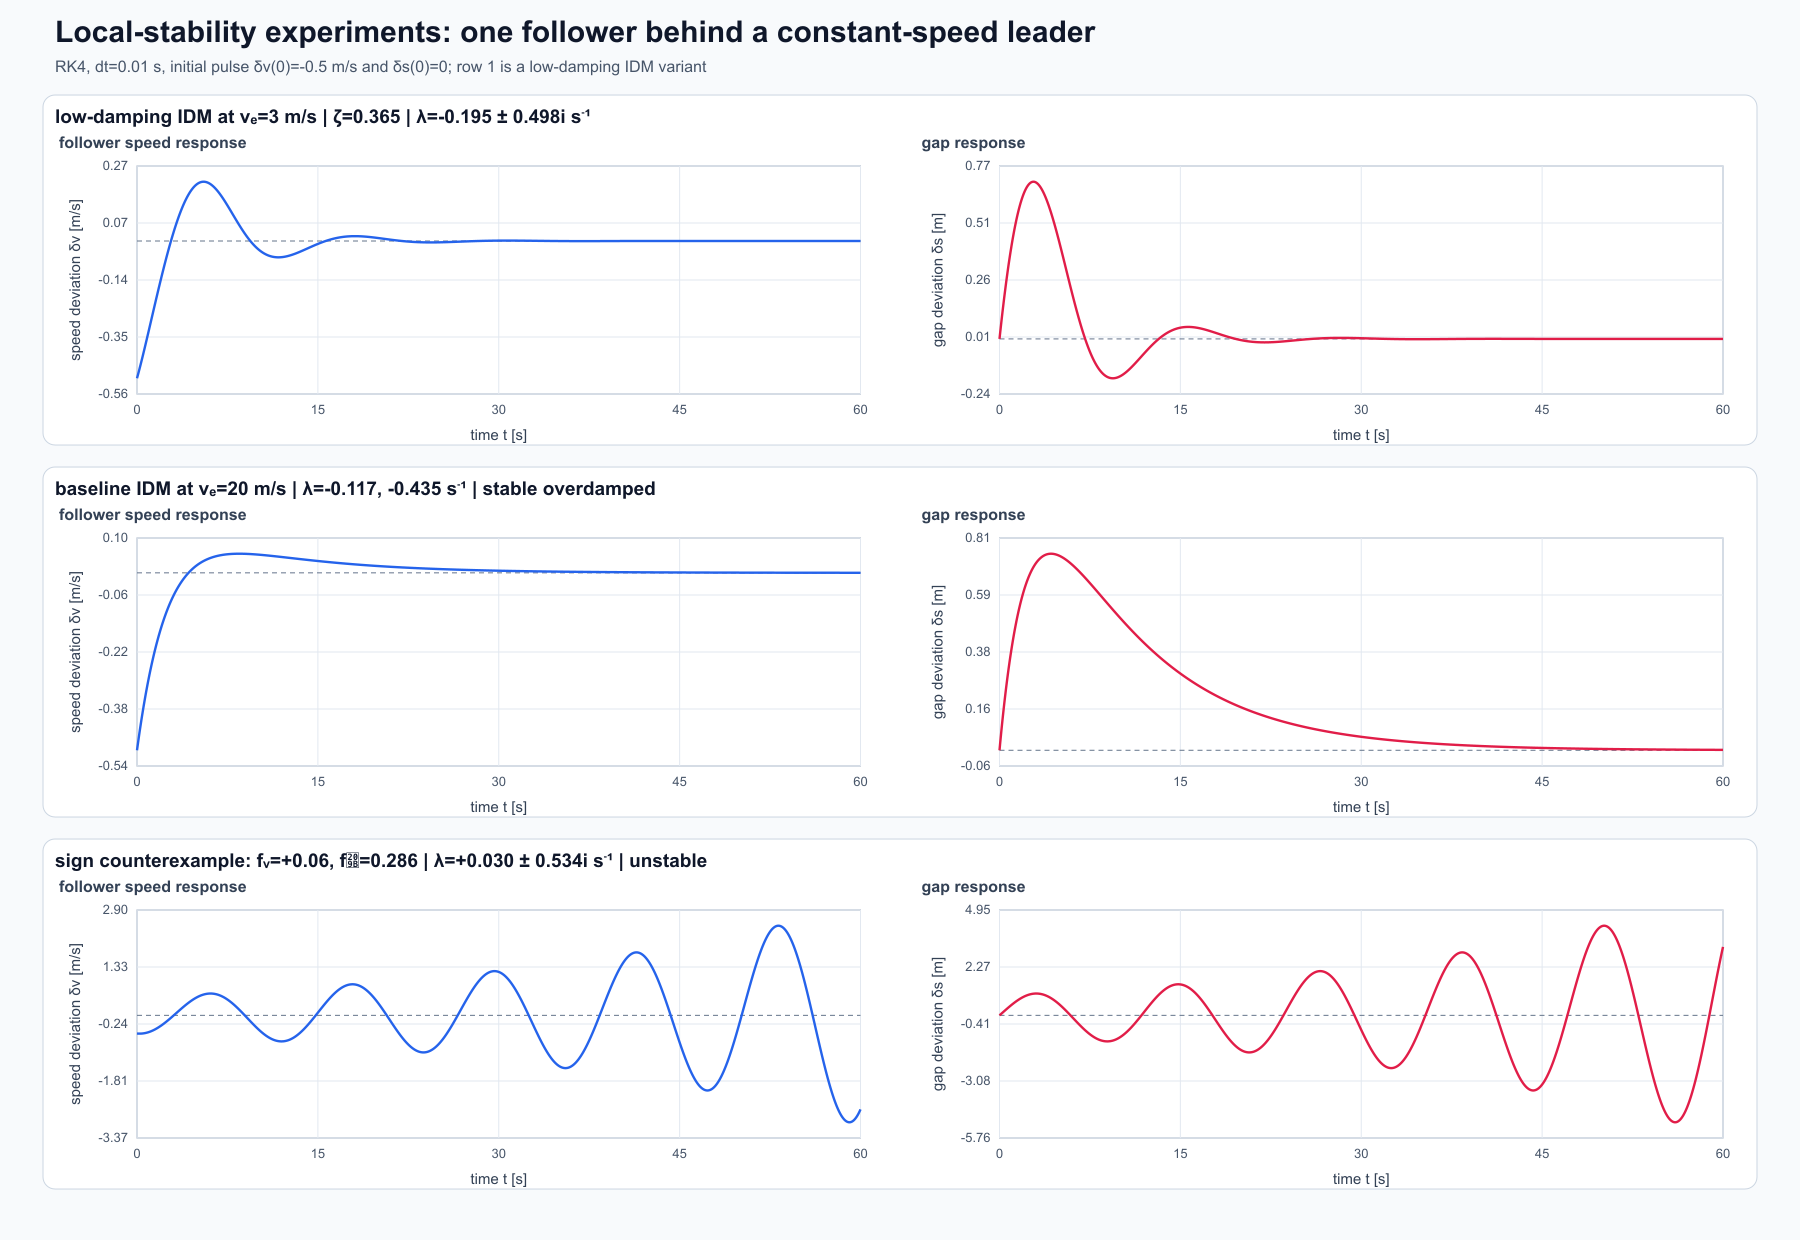
\includegraphics[width=\textwidth]{local_stability_experiments.png}
\caption{Three types of single-vehicle responses regarding local stability.}
\label{fig:localexp}
\figurenote{Three typical root types for local stability and their observable responses. The three rows represent a low-damping IDM, a baseline overdamped IDM, and a case with a sign reversal (leading to instability); the left column shows velocity deviation, the right column shows net gap deviation, and horizontal lines indicate the respective equilibrium values. In the first row, velocity and gap values alternately cross the equilibrium point with peak magnitudes decreasing over time, indicating a pair of conjugate complex roots with negative real parts; this represents a "stable but underdamped" state, where overshoot does not imply instability. In the second row, there is no crossing (or only very weak crossing); two negative real roots mean the recovery is governed by the slow root, demonstrating that overdamping allows for non-oscillatory recovery that is nonetheless slower. In the third row, the peak-to-valley envelope expands over time, corresponding to roots with positive real parts; this proves that even with restorative stiffness, an incorrect sign for velocity damping is sufficient to cause local instability. Since the lead vehicle maintains a constant speed in all three rows, this figure demonstrates whether a single vehicle returns to a given equilibrium point, rather than whether a platoon disturbance amplifies along the vehicle sequence; the latter question must be addressed by the string stability analysis in Chapter ~\ref{sec:string}~.
}
\end{figure}

\begin{tcolorbox}[resultbox,title=\textbf{Conclusions from local tests}]
Local stability addresses only the question of whether a single vehicle eventually recovers. Both IDM scenarios satisfy the conditions for stability ($f_v<0$, $f_s>0$) and thus recover; the damping ratio and the discriminant determine whether the recovery process is oscillatory. The first row exhibits multiple clear overshoots, but the envelope continuously shrinks, indicating stability. This conclusion cannot replace string stability analysis: while the baseline IDM is locally stable for a single vehicle at $v_e=8$ m/s, the same scenario within a long platoon results in disturbances amplifying from vehicle to vehicle (see Figure ~\ref{fig:traj-s0}~).


\end{tcolorbox}

\section{Teaching Example M01: From characteristic roots to RK4 overshoot values}
\sectionstudy{experiment}{Teaching Example M01: From Eigenvalues to RK4 Overshoot}{wilsonward2011,ororsz2010}


\label{sub:m01-local}

Consider a linear local equation that can be verified by hand
\begin{equation}
\delta\ddot s+0.2\,\delta\dot s+0.25\,\delta s=0,
\qquad
\delta s(0)=1\ {\rm m},\quad \delta\dot s(0)=0.
\label{eq:m01-local}
\end{equation}
The two roots are
\[
\lambda_{1,2}=-0.1\pm0.489898\,\mathrm i,
\]





Therefore, the decay time is $10$ s, and the damped oscillation period is

$2\pi/0.489898=12.8255$ s. A point-by-point comparison of the analytical solution with the RK4 solution of $\Delta t=0.05$ s shows

a maximum absolute error of $6.01\times10^{-9}$ m; The first negative overshoot is

$-0.52661$ m. The fact that the curve crosses zero in Figure ~\ref{fig:m01-local} does not indicate instability, because the peak envelope still decays according to

$e^{-0.1t}$.










\begin{figure}[htbp]
\centering
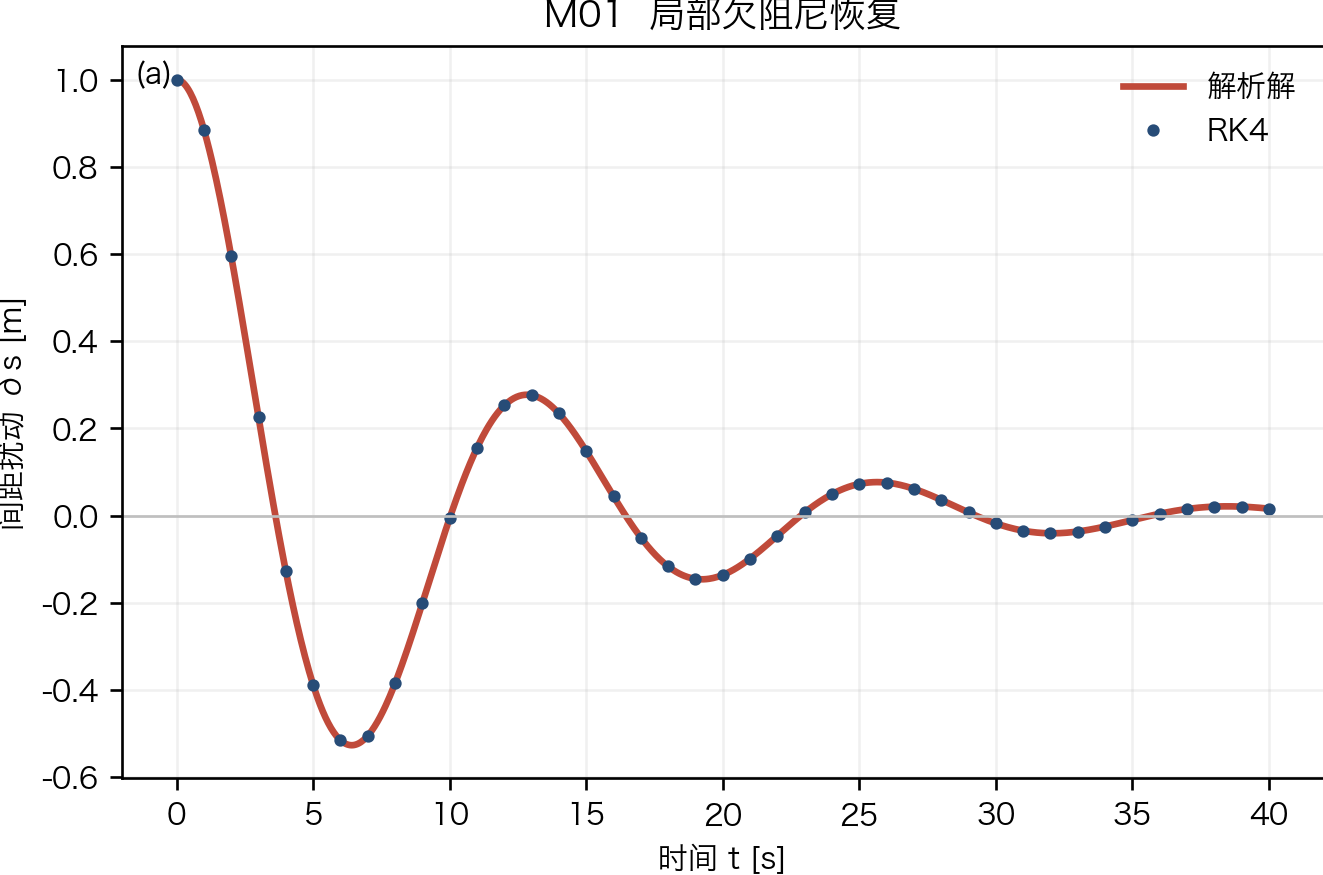
\includegraphics[width=0.86\textwidth]{mini_example_m01.png}
\caption{M01: Local underdamped response.}
\label{fig:m01-local}
\figurenote{Analytical solution and RK4 numerical solution for the same local second-order system in the M01 hand-calculated example. The solid line is reconstructed directly from the characteristic roots, and the discrete data points are obtained through step-by-step integration; the two curves almost coincide in phase, time of first overshoot, and subsequent peak values, indicating consistency among the state definitions, acceleration function, and the four sub-steps of the RK4 method. After the curve first crosses the zero line, a reverse overshoot occurs, followed by exponential decay of the positive and negative peaks; this transforms the “conjugate complex roots” into a directly recognizable damped oscillation. If the numerical points exhibit systematic phase advance, non-decaying peaks, or deviation from the analytical curve, this indicates that the time step is too large or the update order is incorrect—not that a new traffic phenomenon has emerged. This figure therefore demonstrates two things simultaneously: that an underdamped stable response does indeed exist, and that the time integrators used in subsequent simulations in this book can correctly reproduce this response.}
\end{figure}

%==================================================================
\sectionwrapup{Local stability only addresses whether a specific following vehicle can return to equilibrium after the lead vehicle has resumed constant speed. The real part of the second-order root determines the damping, while the imaginary part determines whether oscillation occurs; M01 further illustrates this using the analytical solution and the $6.01\times10^{-9}$ m error of the RK4 method, showing that a response with significant overshoot can still be stable. Local stability does not guarantee that a disturbance will not be amplified as it propagates through the entire train.
}

\chapter{String Stability}
\label{sec:string}
\chapterguide{Why Disturbances Amplify Along the Convoy Even Though Each Vehicle Can Recover}{




This chapter establishes criteria for string stability through three approaches: spatial modes, long-wave expansion, and vehicle-to-vehicle transfer functions. It systematically explains the correspondence between amplitude, wavelength, angular frequency, growth rate, and wave velocity in both theoretical analysis and spatiotemporal diagrams.
}










String stability addresses the following question:




\textbf{Whether a disturbance amplifies or decays as it propagates upstream along the convoy.}

\section{The four fundamental characteristics of a disturbance: amplitude, wavelength, angular frequency, and growth rate}
\sectionstudy{theory}{The four fundamental characteristics of a disturbance: amplitude, wavelength, angular frequency, and growth rate}{swaroop1996,stuedli2017,feng2019}







\label{sub:wavedef}




In linear analysis, a real-valued velocity perturbation can be written as

\begin{equation}
\boxed{
\delta v_n(t)
=A_0e^{\sigma t}
\cos\!\left(kn-\omega t+\phi\right)
}
\label{eq:waveform}
\end{equation}

or in the equivalent complex form

\begin{equation}
\delta v_n(t)
=\operatorname{Re}\!\left\{
A_0e^{i\phi}e^{(\sigma-i\omega)t+ikn}
\right\}.
\end{equation}

This expression breaks down a disturbance into four distinct characteristics:










\begin{center}
\small
\captionof{table}{The amplitude, wavenumber, angular frequency, and growth rate of the disturbance.}
\label{tab:wave-quantities}
\begin{tabular}{p{2.4cm}p{2.4cm}p{4.4cm}p{4.5cm}}
\toprule
\textbf{Characteristics} & \textbf{Symbols/Units} & \textbf{What It Controls} & \textbf{How to Read It} \\
\midrule







Amplitude




& $A_0$，m/s &




 How Strong Is the Initial Perturbation?




&




 Maximum Deviation of the Peak from the Equilibrium Velocity




\\[3pt]
Spatial wavenumber

& $k$，rad/veh &

How rapidly it changes along the vehicle index

&

The larger $k$ is, the shorter the wavelength
\\[3pt]
Angular frequency

& $\omega$，rad/s &

How fast the oscillation appears to a stationary vehicle

&

Period $T_\omega=2\pi/\omega$
\\[3pt]
Growth rate

& $\sigma$，s$^{-1}$ &

Whether the envelope amplifies or decays over time

&

$\sigma>0$ implies growth, $\sigma<0$ implies decay
\\
\bottomrule
\end{tabular}
\end{center}
\tabletext{tab:wave-quantities}{

The four independent characteristics of a linear perturbation and how to interpret them: amplitude describes intensity, wavenumber describes spatial scale, angular frequency describes temporal oscillation, and growth rate determines whether the envelope amplifies or decays; none of these can substitute for the others.
}



Under the complex exponential convention adopted in this book, the complex eigenvalues are
\begin{equation}
\lambda=\sigma-i\omega,
\qquad
\sigma=\operatorname{Re}\lambda,
\qquad
\omega=|\operatorname{Im}\lambda|.
\end{equation}
Therefore\textbf{The angular frequency $\omega$ and the spatial wavenumber $k$ are not the same quantity.}

: $\omega$ describes temporal oscillation, while $k$ describes spatial fluctuation. The two are linked by the dispersion relation $\lambda=\lambda(k)$.

\subsection{Wavenumber and Wavelength}

If measured in terms of vehicle count, the number of vehicles spanned by a complete spatial period is
\begin{equation}
\Lambda_n=\frac{2\pi}{k}
\qquad\text{[veh]}.
\end{equation}
For a loop containing $N$ vehicles, only
\begin{equation}
k_m=\frac{2\pi m}{N},
\qquad
\Lambda_n=\frac{N}{m},
\qquad
m=0,1,\ldots,N-1.
\end{equation}
$m$ represents the number of complete waves within one circuit. If the equilibrium headway is $s_e+l$, the corresponding spatial wavelength is approximately
\begin{equation}
\Lambda_x=(s_e+l)\Lambda_n=\frac{L}{m}.
\end{equation}

For example, when $N=120$ and $v_e=8$ m/s, $s_e+l=19.0355$ m. The dominant mode $m=4$ corresponds to
\begin{equation}
k_4=0.20944\ \text{rad/veh},
\qquad
\Lambda_n=30\ \text{veh},
\qquad
\Lambda_x\approx571.1\ \text{m}.
\end{equation}
This means that four sets of peaks/troughs appear simultaneously on the loop, with each wave set spanning approximately 30 vehicles.

\subsection{Angular Frequency, Period, and Phase Velocity}When observing a specific vehicle (vehicle number $n$), the period with which the pattern \eqref{eq:waveform} repeats over time is
\begin{equation}
T_\omega=\frac{2\pi}{\omega},
\qquad
f=\frac{\omega}{2\pi}\quad\text{[Hz]}.
\end{equation}
Keeping the phase $kn-\omega t+\phi$ constant yields the phase velocity in terms of vehicle number:
\begin{equation}
c_n=\frac{\omega}{k}\quad\text{[veh/s]}.
\end{equation}
Its sign depends on the direction of vehicle numbering and the exponential convention; when converting to wave velocity in road coordinates, the equilibrium motion of the vehicles must also be accounted for. Therefore, this book ultimately relies on the slope of the color bands in the $x$–$t$ plot or the complete phase transformation; one cannot simply multiply $c_n$ by the vehicle spacing to obtain the road wave velocity.

For the example case $m=4$ mentioned above, $|\operatorname{Im}\lambda|=0.12822$ rad/s; thus,
\begin{equation}
T_\omega=49.00\ \text{s},
\qquad
|c_n|=\frac{0.12822}{0.20944}=0.6122\ \text{veh/s}.
\end{equation}
This implies that a stationary probe vehicle experiences a fluctuation of the same phase approximately every 49 seconds, while the wave crest moves in the direction of vehicle indices at a speed of approximately $0.61$ vehicles per second.



\subsection{Why does amplitude not enter into the linear stability criterion?}



Linear equations satisfy the principle of proportional superposition: if $\delta v_n(t)$ is a solution, then $C\delta v_n(t)$ is also a solution. Consequently, within the linear regime, scaling the initial amplitude $A_0$ by a factor of 10 merely scales the entire response curve by a factor of 10;

\textbf{it does not change}$\lambda(k)$, $\sigma$, $\omega$, or critical parameters. The amplitude evolves as
\begin{equation}
A(t)=A_0e^{\sigma t}.
\end{equation}
For example, the $m=4$ mode of the baseline IDM exhibits $\sigma=0.00408566$ s$^{-1}$ at $v_e=8$ m/s. If $A_0=0.002$ m/s, then under linear prediction,
\begin{equation}
A(300)=0.002e^{0.00408566\times300}=0.00682\ \text{m/s}.
\end{equation}
Changing $A_0$ does not alter the exponential slope $0.00408566$; however, once the amplitude becomes large enough to cause the vehicle to approach a standstill, reach minimal spacing, or hit acceleration saturation, nonlinear terms come into play, and the growth no longer strictly follows an exponential law. Therefore, all quantitative stability experiments must report both the initial amplitude and the time window used for fitting.



\begin{tcolorbox}[notebox,title=\textbf{"What is being swept" in open-chain frequency sweeps versus ring-road modal scans}]
\begin{itemize}[leftmargin=1.4em,itemsep=3pt]
\item \textbf{Open-chain transfer function experiment:}

The temporal angular frequency $\omega$ is artificially prescribed for the lead vehicle, and the vehicle-to-vehicle amplitude ratio $|G(i\omega)|$ and phase difference are measured; here, the temporal frequency is the parameter being swept.


\item \textbf{Ring-road eigenvalue experiment:}

The discrete spatial wavenumber $k_m$ is specified first, and $\lambda_m=\sigma_m-i\omega_m$ is then determined via the dispersion relation; here, the spatial wavelength is the parameter being swept.\item The two approaches examine different facets of the same propagation problem. In a uniform unidirectional model, they can be interconverted via $G(\lambda)=e^{ik}$; however, this simple conversion may fail in the presence of bidirectional coupling or heterogeneity.


\end{itemize}
\end{tcolorbox}

\begin{tcolorbox}[experimentbox,title=\textbf{Proposed experiments on three sets of perturbation characteristics}]
\begin{enumerate}[leftmargin=1.6em,itemsep=3pt]
\item \textbf{Wavelength sweep:}

Fix the amplitude at a low level and sequentially inject $m=1,2,\ldots,N/2$; compare the measured growth rate with $\operatorname{Re}\lambda(k_m)$ to identify the most unstable wavelength.


\item \textbf{Angular frequency sweep:}

In an open-chain configuration, subject the lead vehicle to sinusoidal perturbations with varying $\omega$, measure $|Y_n/Y_{n-1}|$, and plot the amplification frequency band.


\item \textbf{Amplitude sweep:}

Apply $A_0=0.002,0.02,0.2$ m/s for a given $k_m$. At low amplitudes, the three $\ln A(t)$ curves should be parallel; a lack of parallelism indicates the system has moved beyond the linear regime.


\end{enumerate}
\end{tcolorbox}

\section{Method 1: Long-wave expansion}
\sectionstudy{theory}{Method 1: Long-wave expansion}{swaroop1996,stuedli2017,feng2019}Switching to the position perturbation $y_n = \delta x_n$, we have $\delta s_n = y_{n-1}-y_n$ and $\delta v_n = \dot y_n$:
\begin{equation}
\ddot y_n = f_s\left(y_{n-1}-y_n\right) + f_v\,\dot y_n + f_{v_l}\,\dot y_{n-1}
\end{equation}

Assume a traveling wave solution $y_n(t) = \hat y\,e^{\lambda t + ikn}$; then, with $y_{n-1}=y_n e^{-ik}$, we obtain the dispersion relation:
\begin{equation}
\lambda^2 = f_s\left(e^{-ik}-1\right) + \left(f_v + f_{v_l}e^{-ik}\right)\lambda
\label{eq:disp}
\end{equation}

Instability first appears in long waves ($k\to 0$). Let $\varepsilon = -ik$, expand $\lambda = c_1\varepsilon + c_2\varepsilon^2 + \cdots$, and—utilizing $e^{\varepsilon}=1+\varepsilon+\tfrac{\varepsilon^2}{2}+\cdots$—match order by order:



\textbf{Order $O(\varepsilon)$:}


\begin{equation}
0 = f_s + \left(f_v+f_{v_l}\right)c_1
\qquad\Longrightarrow\qquad
c_1 = -\frac{f_s}{f_v+f_{v_l}} = V'(s_e)
\end{equation}
That is, $c_1$ is the kinematic wave speed, consistent with equation \eqref{eq:Vprime}.



\textbf{Order $O(\varepsilon^2)$:}\begin{equation}
c_1^2 = \frac{f_s}{2} + f_{v_l}c_1 + \left(f_v+f_{v_l}\right)c_2
\qquad\Longrightarrow\qquad
c_2 = \frac{c_1^2 - \frac12 f_s - f_{v_l}c_1}{f_v+f_{v_l}}
\end{equation}

From $\lambda = -i c_1 k - c_2 k^2$, we obtain $\operatorname{Re}\lambda = -c_2 k^2$; the stability requirement is $c_2\ge 0$. Since the denominator is $f_v+f_{v_l}<0$, the numerator must be non-positive:
\begin{equation}
c_1^2 - \tfrac12 f_s - f_{v_l}c_1 \le 0
\end{equation}

Substituting $c_1$ and multiplying by $\left(f_v+f_{v_l}\right)^2/f_s > 0$:
\begin{equation}
f_s + f_{v_l}\left(f_v+f_{v_l}\right) - \tfrac12\left(f_v+f_{v_l}\right)^2 \le 0
\end{equation}

Noting that
\begin{equation}
f_{v_l}\left(f_v+f_{v_l}\right) - \tfrac12\left(f_v+f_{v_l}\right)^2
= \left(f_v+f_{v_l}\right)\cdot\frac{f_{v_l}-f_v}{2}
= \frac{f_{v_l}^2 - f_v^2}{2}
\end{equation}

we obtain


\begin{tcolorbox}[keybox,title=\textbf{String stability condition (long-wave)}]
\begin{equation}
\frac{1}{2}\left(f_v^2 - f_{v_l}^2\right) \;\ge\; f_s
\label{eq:string}
\end{equation}
\end{tcolorbox}

\subsection{Why the original car-following model first undergoes long-wave instability}\label{sub:why-long-wave-first}

The fact that "long-wave instability occurs first" is not inferred from simulation images but is determined by the spectral structure near $k=0$. Let
\begin{equation}
\mu=f_v+f_{v_l}<0,
\qquad
\Phi=\frac{f_v^2-f_{v_l}^2}{2}-f_s .
\end{equation}
Substituting $k=0$ into the dispersion relation \eqref{eq:disp} yields
\begin{equation}
\lambda(\lambda-\mu)=0,
\qquad
\lambda_0=0,\qquad \lambda_f=\mu<0 .
\label{eq:k0roots}
\end{equation}
where $\lambda_f$ represents a rapidly decaying single-vehicle relaxation mode; $\lambda_0=0$ arises from translational invariance: shifting the positions of all vehicles on the ring by the same constant does not alter any gaps or accelerations, so the system must possess a zero root that neither grows nor decays. The long-wave branch extends continuously from this zero root; consequently, it lies close to the imaginary axis and is the most likely to cross the stability boundary first as parameters vary.

Further rearranging the preceding $c_2$ yields
\begin{equation}
c_2=-\frac{f_s}{\mu^3}\,\Phi,
\qquad
\lambda(k)=-ic_1k-c_2k^2+O(k^3),
\qquad
c_1=-\frac{f_s}{\mu}=V'(s_e).
\label{eq:longwave-branch}
\end{equation}
Given $\mu^3<0$ and the coefficient $-f_s/\mu^3>0$, $c_2$ shares the same sign as $\Phi$:
\begin{equation}
\Phi>0\Rightarrow\operatorname{Re}\lambda\simeq-c_2k^2<0,
\qquad
\Phi<0\Rightarrow\operatorname{Re}\lambda\simeq-c_2k^2>0.
\end{equation}
Once $\Phi$ changes from positive to negative, any sufficiently small but non-zero $k$ immediately acquires a positive growth rate. Strictly speaking,

\textbf{it is not $k=0$ itself that becomes unstable}...remains a neutral overall translation; instead, the long-wave branches of $k\to0$ and $k\ne0$ are the first to enter the right half-plane.

This conclusion can also be expressed as an equivalent long-wave partial differential equation. If $r(n,t)$ represents a slowly varying spacing perturbation, the linear principal part is
\begin{equation}
r_t+c_1r_n=c_2r_{nn}+\cdots .
\label{eq:effective-diffusion}
\end{equation}
$c_1$ merely transports the perturbation; when $c_2>0$, $r_{nn}$ smooths out fluctuations like normal diffusion; when $c_2<0$, it acts as "anti-diffusion," where broad, gentle fluctuations are amplified. The difference in long-wave values between adjacent vehicles is only
\begin{equation}
e^{-ik}-1=-ik-\frac{k^2}{2}+O(k^3),
\end{equation}
Both the restoring and dissipative signals are weak, with a net damping of only $O(k^2)$; in contrast, the difference between adjacent vehicles for short waves is $O(1)$, which is more easily suppressed by local velocity damping. This is why long waves are physically more dangerous.



\begin{tcolorbox}[notebox,title=\textbf{Why this instability might go "unnoticed" on a finite-sized loop}]
The loop allows only $k_m=2\pi m/N$. The most dangerous continuous long waves occur at $k\to0$, but the smallest non-zero wavenumber attainable with a finite number of vehicles is $k_{\min}=2\pi/N$; if $N$ is too small, the first discrete point may skip over the range of positive growth rates, leading a simulation to mistakenly classify an inherently unstable platoon of infinite length as stable. Section E5 of Chapter \ref{sec:appx} provides a quantitative test of this effect.\end{tcolorbox}

\subsection{Teaching Example M02: Why the same IDM model is stable with 12 vehicles but unstable with 20}


\label{sub:m02-finite-ring}

Keep the original IDM and $v_e=8$ m/s fixed, and vary only the number of vehicles on the ring road. For each permissible wavenumber
$k_m=2\pi m/N$, calculate the two roots and take the maximum real part:


\begin{center}
\small
\captionof{table}{M02: Lowest discrete modes for different numbers of vehicles.}
\label{tab:m02-finite-ring}
\begin{tabular}{rccc}
\toprule
$N$ &

Dominant mode $m^*$

&

Wavelength [vehicles]

& $\max\operatorname{Re}\lambda$ [s$^{-1}$] \\
\midrule
12 & 1 & 12 & $-0.0210366$ \\
20 & 1 & 20 & $+0.00130121$ \\
30 & 1 & 30 & $+0.00408566$ \\
\bottomrule
\end{tabular}
\end{center}
\tabletext{tab:m02-finite-ring}{

Permissible dominant wavelengths and growth rates for the same IDM operating point at $N=12,20,30$. When the number of vehicles increases from 12 to 20, the lowest non-zero wavenumber enters the long-wave instability region; thus, stability on a finite ring road does not directly imply stability for an infinite platoon.
}


With the same set of parameters at $N=12$, the first non-zero wavenumber still falls within the negative growth region; by $N=20$,
$k_{\min}$ is close enough to zero to finally sample a long wave with positive growth. Therefore, the fact that "no stop-and-go waves appeared on the 12-vehicle ring road"
does not imply stability for an infinite platoon; it only implies that for that small ring road,

\textbf{the three permissible modes}

did not grow.



\begin{figure}[htbp]
\centering
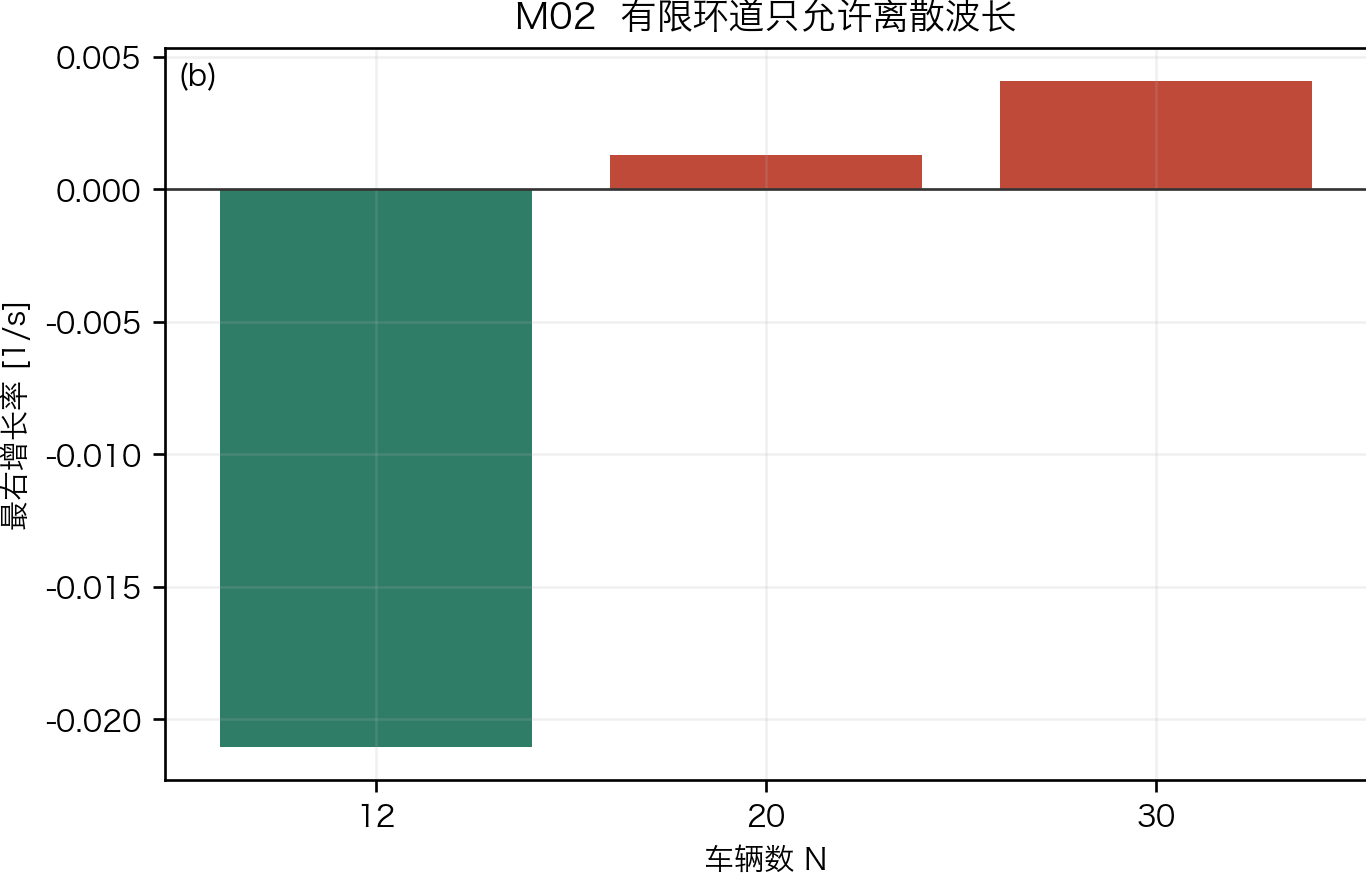
\includegraphics[width=0.82\textwidth]{mini_example_m02.png}
\caption{M02: Discrete wavelength effects on a finite ring road.}
\label{fig:m02-finite-ring}
\figurenote{M02: Spectral analysis of discrete modes in a finite ring. Each bar corresponds to the real part of the rightmost eigenvalue; green indicates mode decay, while red indicates growth over time. Different panels vary only the number of vehicles ($N$); IDM parameters and the equilibrium operating point remain identical. In small rings, the lowest non-zero wavenumber is relatively high, preventing the closure of dangerous, extremely long waves; consequently, all bars may remain green. As $N$ increases, the eigenvalue moves toward zero, and the first red bar to appear corresponds to the lowest-order long wave. This phenomenon demonstrates that the finite ring is not merely an unbiased scaled-down version of the infinite platoon criterion: it systematically overestimates stability due to the absence of sufficiently long wavelengths. The position of the red bar indicates the vehicle scale that will dominate the stop-and-go waves in the time domain; therefore, experimental reports must specify $N$ rather than merely reporting density and IDM parameters.}
\end{figure}

\begin{tcolorbox}[notebox,title=\textbf{Applicability limits: Not all extended models lose long-wave stability first.}]
The aforementioned "initial long-wave instability" holds true for the

\textbf{basic, homogeneous, unidirectional, delay-free}

model; furthermore, the transfer function analysis in the next section will confirm that the most dangerous frequency is indeed the lowest non-zero mode. However, when the lead-vehicle acceleration gain is excessive, or when look-back coupling, time delays, or discrete control are present, finite-wavelength or finite-frequency branches may cross the imaginary axis first. In such cases, one must scan the entire wavenumber or frequency range rather than checking only the specific mode associated with the lowest wavenumber.

\end{tcolorbox}

\section{Method 2: Transfer Function Method}
\sectionstudy{theory}{Method 2: Transfer Function Method}{swaroop1996,ploeg2014,feng2019}The long-wave expansion only guarantees decay within the neighborhood of $k\to0$. To determine that

\textbf{disturbances of all wavelengths}

do not amplify, a frequency-domain approach is required. This subsection details every step of the process.



\subsection{Step 1: Justification for using the Laplace transform}



The linearized equation for positional perturbation,
\begin{equation}
\ddot y_n = f_s\left(y_{n-1}-y_n\right) + f_v\,\dot y_n + f_{v_l}\,\dot y_{n-1}
\label{eq:ylin}
\end{equation},

\textbf{is a linear differential equation with constant coefficients}

(where the coefficients $f_s,f_v,f_{v_l}$ are constants evaluated at the equilibrium point), and its structure is identical for every $n$. These two factors ensure that the Laplace transform is applicable and that the resulting input-output ratio is independent of the vehicle index $n$.

Assume the platoon is initially in an equilibrium state, adopt zero initial conditions
\begin{equation}
y_n(0) = 0, \qquad \dot y_n(0) = 0 \qquad \forall n
\end{equation},
and let $Y_n(\lambda) = \mathcal{L}\{y_n(t)\} = \int_0^\infty y_n(t)\,e^{-\lambda t}\,\mathrm{d}t$. Under zero initial conditions, the transformation rule for differentiation is
\begin{equation}
\mathcal{L}\{\dot y_n\} = \lambda Y_n - y_n(0) = \lambda Y_n,
\qquad
\mathcal{L}\{\ddot y_n\} = \lambda^2 Y_n - \lambda y_n(0) - \dot y_n(0) = \lambda^2 Y_n
\end{equation}



\subsection{Step 2: Transformation and derivation of the transfer function}Transforming both sides of equation ~\eqref{eq:ylin} term by term:
\begin{equation}
\lambda^2 Y_n = f_s\left(Y_{n-1}-Y_n\right) + f_v\,\lambda Y_n + f_{v_l}\,\lambda Y_{n-1}
\end{equation}

Move all terms containing $Y_n$ to the left side and all terms containing $Y_{n-1}$ to the right side:
\begin{equation}
\lambda^2 Y_n + f_s Y_n - f_v\lambda Y_n = f_s Y_{n-1} + f_{v_l}\lambda Y_{n-1}
\end{equation}

Factor out common terms on both sides:
\begin{equation}
\left(\lambda^2 - f_v\lambda + f_s\right) Y_n = \left(f_{v_l}\lambda + f_s\right) Y_{n-1}
\end{equation}

Taking the ratio yields

\textbf{Vehicle-to-vehicle transfer function}：
\begin{tcolorbox}[keybox,title=\textbf{Vehicle-to-vehicle transfer function}]
\begin{equation}
G(\lambda) \;=\; \frac{Y_n(\lambda)}{Y_{n-1}(\lambda)}
\;=\; \frac{f_s + f_{v_l}\lambda}{\lambda^2 - f_v\lambda + f_s}
\label{eq:G0}
\end{equation}
\end{tcolorbox}



Three observations:



\begin{itemize}[leftmargin=1.4em,itemsep=3pt]
\item \textbf{The denominator is precisely the characteristic polynomial for local stability}

(see equation ~\eqref{eq:char}). Therefore, for local stability, the poles of $\iff$ lie in the left half-plane, making $G$ a stable transfer function. This is a prerequisite for the meaningful discussion of $\left|G\right|$: if $G$ were unstable, the response of a single vehicle would already diverge, rendering the concept of "disturbance amplification factor" meaningless.


\item \textbf{$G$ is independent of $n$}

(uniform platoon), so disturbances are multiplied stage by stage:
\begin{equation}
Y_n = G(\lambda)\,Y_{n-1} = G^2(\lambda)\,Y_{n-2} = \cdots = G^{\,n}(\lambda)\,Y_0
\end{equation}\item \textbf{Position, velocity, and spacing share the same $G$.}

Velocity perturbation $\mathcal{L}\{\delta v_n\} = \lambda Y_n$ ($\lambda$ cancels out when taking the ratio); spacing perturbation $\mathcal{L}\{\delta s_n\} = Y_{n-1}-Y_n$; then
\[
\frac{\mathcal{L}\{\delta s_{n+1}\}}{\mathcal{L}\{\delta s_n\}}
= \frac{Y_n - Y_{n+1}}{Y_{n-1}-Y_n}
= \frac{G\left(Y_{n-1}-Y_n\right)}{Y_{n-1}-Y_n} = G
\]





Therefore, there is no need to distinguish which variable is used to define linear stability.







\end{itemize}

\subsection{Step 3: Why is the criterion $\left|G(i\omega)\right|\le1$?}










Based on $Y_n = G^{\,n}Y_0$, take $\lambda = i\omega$ (i.e., examine the steady-state response to a sinusoidal disturbance with frequency $\omega$):

\begin{equation}
\left|Y_n(i\omega)\right| = \left|G(i\omega)\right|^{\,n}\left|Y_0(i\omega)\right|
\end{equation}




Thus: If there exists a frequency $\omega^\star$ such that $\left|G(i\omega^\star)\right|>1$, this frequency component propagates along the convoy




\textbf{is amplified geometrically}




; after propagating upstream through several vehicles, it will inevitably exceed the linear range and develop into a stop-and-go wave. Conversely, if the gain for all frequencies does not exceed 1, no disturbance (which, according to the Fourier decomposition, is the sum of various frequencies) will be amplified.










\begin{tcolorbox}[keybox,title=\textbf{Strict Definition of Linear Stability}]
\[
\text{String-stable}
\iff
\left\|G\right\|_{\infty} \equiv \sup_{\omega\in\mathbb{R}}\left|G(i\omega)\right| \;\le\; 1
\quad\text{and}\quad G\ \text{stable (locally stable)}
\]
\end{tcolorbox}

\subsection{Step 4: Calculate $\left|G(i\omega)\right|^2$}





Substitute $\lambda = i\omega$ into the expression ~\eqref{eq:G0}, and separate the numerator and denominator into real and imaginary parts, respectively.










\textbf{Numerator.}
\begin{equation}
N(i\omega) = f_s + f_{v_l}\,(i\omega) = \underbrace{f_s}_{\text{real part}} + i\underbrace{f_{v_l}\omega}_{\text{imaginary part}}
\qquad\Longrightarrow\qquad
\left|N\right|^2 = f_s^2 + f_{v_l}^2\omega^2
\end{equation}

\textbf{Numerator.}




Note $(i\omega)^2 = i^2\omega^2 = -\omega^2$:

\begin{equation}
D(i\omega) = (i\omega)^2 - f_v(i\omega) + f_s
= \underbrace{\left(f_s-\omega^2\right)}_{\text{real part}} + i\underbrace{\left(-f_v\omega\right)}_{\text{imaginary part}}
\end{equation}

\begin{equation}
\left|D\right|^2 = \left(f_s-\omega^2\right)^2 + f_v^2\omega^2
\end{equation}




(The imaginary part is squared, causing the negative sign to disappear; therefore, it is written as $f_v^2\omega^2$.)




Therefore,

\begin{equation}
\left|G(i\omega)\right|^2 = \frac{\left|N\right|^2}{\left|D\right|^2}
= \frac{f_s^2 + f_{v_l}^2\omega^2}{\left(f_s-\omega^2\right)^2 + f_v^2\omega^2}
\end{equation}




The condition $\left|G\right|\le1$ is equivalent to $\left|G\right|^2\le1$, that is, $\left|N\right|^2\le\left|D\right|^2$:







\begin{tcolorbox}[keybox,title=\textbf{Magnitude condition}]
\begin{equation}
f_s^2 + f_{v_l}^2\omega^2
\;\le\;
\left(f_s-\omega^2\right)^2 + f_v^2\omega^2
\end{equation}
\end{tcolorbox}

\subsection{Step 5: Simplify}










Rearrange the terms by subtracting the left side from the right side:

\begin{equation}
\left|D\right|^2 - \left|N\right|^2
= \underbrace{f_s^2 - 2f_s\omega^2 + \omega^4}_{\left(f_s-\omega^2\right)^2} + f_v^2\omega^2 - f_s^2 - f_{v_l}^2\omega^2 \;\ge\; 0
\end{equation}




$f_s^2$ cancels out, and since every remaining term contains $\omega^2$, factor out the common factor:

\begin{equation}
\omega^2\left[\omega^2 - 2f_s + f_v^2 - f_{v_l}^2\right] \;\ge\; 0
\label{eq:bracket}
\end{equation}




Since $\omega^2\ge0$ holds true for all values, the condition reduces to the expression in parentheses being non-negative. The expression in parentheses is $\omega^2$’s




\textbf{monotonically increasing}The function attains its minimum value at $\omega\to0$; therefore, it holds for all $\omega$ if and only if

\begin{equation}
f_v^2 - f_{v_l}^2 - 2f_s \;\ge\; 0
\end{equation}




that is, the expression ~\eqref{eq:string}. This also indicates that the condition is




\textbf{necessary and sufficient}




, and




\textbf{the most dangerous frequency is $\omega\to0$}




—which corroborates the conclusions of the long-wave analysis.










\begin{tcolorbox}[notebox,title=\textbf{Why is the equality sign always used at $\omega=0$}]

The expression ~\eqref{eq:bracket} is always 0 at $\omega=0$, corresponding to $\left|G(0)\right| = f_s/f_s = 1$. This is no coincidence: $\lambda=0$ represents “a constant shift in the positions of all cars as a whole,” which is itself a valid new equilibrium state that neither amplifies nor attenuates the signal. Therefore, the $\left|G\right|$ curve always starts at 1, and whether it is stable depends on whether




\textbf{it moves up or down after departing from 1}




. Expanding the small $\omega$:

\[
\left|G(i\omega)\right|^2 \approx 1 + \frac{2f_s + f_{v_l}^2 - f_v^2}{f_s^2}\,\omega^2 + O(\omega^4)
\]

A negative coefficient in $\omega^2$ indicates stability—this is precisely the same condition.







\end{tcolorbox}

\subsection{Addendum: Equivalence between the transfer function and the dispersion relation}





These two methods are essentially the same. Rearranging the dispersion relation of equation ~\eqref{eq:disp} yields:

\begin{equation}
\left(\lambda^2 - f_v\lambda + f_s\right) = e^{-ik}\left(f_s + f_{v_l}\lambda\right)
\qquad\Longleftrightarrow\qquad
G(\lambda) = e^{\,ik}
\end{equation}




That is:




\textbf{The dispersion relation is given by the equation $G(\lambda)=e^{ik}$
}




. The neutral stable curve $\operatorname{Re}\lambda=0$ corresponds to $\left|G\right|=1$. The long-wave expansion involves solving this equation at $k\to0$, while the transfer function method involves directly scanning the entire $\lambda=i\omega$ axis—the latter is more comprehensive, a point that becomes critical in Chapter ~\ref{sec:lead}~ when considering vehicle acceleration.










\section{Expressed in terms of primitive partial derivatives}
\sectionstudy{theory}{Expressed in terms of primitive partial derivatives}{swaroop1996,stuedli2017,feng2019}










Substitute back into $f_v = F_v+F_{\dv}$ and $f_{v_l}=-F_{\dv}$:







\begin{tcolorbox}[keybox]
\begin{equation}
\frac{1}{2}F_v^2 + F_v F_{\dv} - F_s \;\ge\; 0
\end{equation}
\end{tcolorbox}










Note that $F_v<0$ and $F_{\dv}<0$ hold, so $F_vF_{\dv}>0$ also holds:




\textbf{The relative velocity feedback term always acts as a stabilizing factor.}

\begin{tcolorbox}[notebox,title=\textbf{Verification: Degenerate to OVM}]

The optimal speed model $\dot v = \left[V(s)-v\right]/\tau$ includes $F_s = V'/\tau$, $F_v=-1/\tau$, and $F_{\dv}=0$; the conditions degenerate into

\[
V'(s_e) \le \frac{1}{2\tau}
\]

, consistent with classical results.







\end{tcolorbox}

%==================================================================
\sectionwrapup{Linear stability requires that perturbations at any frequency are not amplified as they propagate from car to car; equivalently, it requires that all non-trivial spatial modes in the ring track do not grow. Amplitude, angular frequency, wavelength, phase velocity, and growth rate describe different observations, respectively; The long-wave threshold is derived from $k\to0$; for a finite number of cars, only discrete wavenumbers are sampled.}

\chapter{Substituting into the IDM}
\label{sec:idm}
\chapterguide{How the general criterion is transformed into the computable IDM stability region}{




This chapter calculates the IDM equilibrium relations and partial derivatives, expressing the abstract conditions as functions of velocity, density, and model parameters. Readers should master the computational chain from parameters to the neutral boundary and understand that “physically reasonable parameters” do not necessarily imply “stability across all operating conditions.”
}

\section{Models and Equilibrium States}
\sectionstudy{model}{Models and Equilibrium States}{treiber2000,sugiyama2008,treiberkesting2013}










\begin{equation}
\dot v = a\left[1 - \left(\frac{v}{v_0}\right)^{\delta} - \left(\frac{s^*(v,\dv)}{s}\right)^{2}\right],
\qquad
s^* = s_0 + vT + \frac{v\,\dv}{2\sqrt{ab}}
\end{equation}




At equilibrium, $\dv=0$, therefore $s_e^* = s_0+v_eT$. Let $\dot v=0$:

\begin{equation}
\left(\frac{s_e^*}{s_e}\right)^2 = 1-\left(\frac{v_e}{v_0}\right)^{\delta}
\qquad\Longrightarrow\qquad
s_e(v_e) = \frac{s_0+v_eT}{\sqrt{1-\left(v_e/v_0\right)^{\delta}}}
\end{equation}




Let

\begin{equation}
z \equiv \frac{s_e^*}{s_e} = \sqrt{1-\left(\frac{v_e}{v_0}\right)^{\delta}} \in (0,1]
\end{equation}










\section{Three Partial Derivatives}
\sectionstudy{theory}{Three Partial Derivatives}{treiber2000,sugiyama2008,treiberkesting2013}

\begin{align}
F_s &= \frac{2a\left(s_e^*\right)^2}{s_e^3} = \frac{2az^2}{s_e} \\[6pt]
F_v &= -\underbrace{\frac{a\delta}{v_0}\left(\frac{v_e}{v_0}\right)^{\delta-1}}_{\textstyle A}
       \;-\;\underbrace{\frac{2azT}{s_e}}_{\textstyle B}
       \qquad\left(\text{because } \left.\frac{\partial s^*}{\partial v}\right|_e = T\right) \\[6pt]
F_{\dv} &= -\frac{2a\,s_e^*}{s_e^2}\cdot\frac{v_e}{2\sqrt{ab}}
       = -\underbrace{\sqrt{\frac{a}{b}}\,\frac{z\,v_e}{s_e}}_{\textstyle C}
\end{align}

\section{Stability Conditions for IDM}
\sectionstudy{model}{Stability Conditions for IDM}{treiber2000,treiberkesting2013}

\textbf{Local Stability.}




 $F_s>0$ and $f_v = F_v+F_{\dv} = -(A+B+C)<0$. As long as $v_e<v_0$ (i.e., $z>0$) holds, both are always true.










\begin{tcolorbox}[notebox]
\textbf{The IDM is always locally stable along the entire equilibrium branch}




, but is underdamped when $(A+B+C)^2<4F_s$, manifesting as damped oscillations.







\end{tcolorbox}

\textbf{Linear Stability.}
\begin{tcolorbox}[keybox,title=\textbf{IDM Linear Stability Criteria}]

\begin{equation}
\Phi(v_e) \equiv \frac{1}{2}(A+B)^2 + (A+B)\,C - F_s \;\ge\; 0
\label{eq:idmphi}
\end{equation}

where

\[
A = \frac{a\delta}{v_0}\left(\frac{v_e}{v_0}\right)^{\delta-1},
\qquad
B = \frac{2azT}{s_e},
\qquad
C = \sqrt{\frac{a}{b}}\,\frac{z\,v_e}{s_e}
\]

\[
z = \sqrt{1-\left(v_e/v_0\right)^{\delta}},
\qquad
s_e = \frac{s_0+v_eT}{z}
\]







\end{tcolorbox}

\section{Two Limits}
\sectionstudy{theory}{Two Limits}{treiber2000,sugiyama2008,treiberkesting2013}

\textbf{Free-Flow Limit $v_e\to v_0$.}




 At this point, $z\to 0$, $F_s\to 0$, $B\to 0$, and $C\to 0$ are all infinite, while $A$ remains a finite positive value; therefore, $\Phi\to\tfrac12A^2>0$:\textbf{Constant Line Stable}。

\textbf{Congestion Limit $v_e\to 0$.}




 At this point, $z\to1$, $s_e\to s_0$, $A\to0$ ($\delta>1$), $C\to0$, and $B\to 2aT/s_0$ are conditioned to

\begin{equation}
\frac{1}{2}\left(\frac{2aT}{s_0}\right)^2 \ge \frac{2a}{s_0}
\qquad\Longleftrightarrow\qquad
\frac{aT^2}{s_0} \ge 1
\end{equation}




This explains why the IDM is extremely sensitive to $T$, $a$, and $s_0$ in stop-and-go traffic.




%==================================================================







\sectionwrapup{Substituting the IDM’s equilibrium relations and the three partial derivatives into the general criterion yields the local and linear stability boundaries as a function of speed. The low-speed limit shows that $T$, $a$, and $s_0$ directly control the stability margin; physically reasonable parameters do not necessarily imply linear stability at all densities.}

\chapter{Numerical Examples}
\label{sec:num}
\chapterguide{How Theoretical Predictions Are Verified by Reproducible Experiments}{




This chapter presents both stable and unstable operating conditions under uniform parameters, using growth rates, dominant modes, position-time velocity-colored trajectories, and specified vehicle speed/spacing curves to cross-validate the theory, thereby establishing a standard for interpreting the figures in subsequent examples throughout the book.}

\begin{center}
\captionof{table}{Reference IDM parameters used for numerical experiments throughout this book.}
\label{tab:baseline-idm-parameters}
\begin{tabular}{lcccccccc}
\toprule







Parameter




& $v_0$ & $T$ & $s_0$ & $a$ & $b$ & $\delta$ & $l$ \\
\midrule







Value




& 33.3 m/s & 1.5 s & 2 m & 1 m/s$^2$ & 1.5 m/s$^2$ & 4 & 5 m \\
\bottomrule
\end{tabular}
\end{center}
\tabletext{tab:baseline-idm-parameters}{




Unified reference values for desired speed, time interval, minimum spacing, acceleration/deceleration, and vehicle length. Unless otherwise specified, these parameters are used in subsequent scenarios; therefore, comparisons between different mechanisms will not be confounded by variations in parameter settings.
}










Scanning Equation ~\eqref{eq:idmphi} across the entire speed range yields two critical points:










\begin{center}
\captionof{table}{Two critical operating points in the IDM’s unstable speed band.}
\label{tab:idm-critical-points}
\begin{tabular}{lccccc}
\toprule







Critical points




& $v_e$ & $s_e$ &




 Headway $s_e+l$




&




 Density $\rho$




&




Traffic Flow $Q$



\\
\midrule







Lower Critical




& 0.91 m/s & 3.36 m & 8.36 m & 119.6 veh/km & 391 veh/h \\







Upper Critical Point




& 18.61 m/s & 31.50 m & 36.50 m & 27.4 veh/km & 1836 veh/h \\
\bottomrule
\end{tabular}
\end{center}
\tabletext{tab:idm-critical-points}{




The velocities, spacing, density, and flow rate corresponding to the lower and upper critical points. This converts the analytical stability boundaries in the velocity domain into road performance indicators and indicates that the upper critical point is approaching the base-map capacity region.
}

\begin{tcolorbox}[notebox,title=\textbf{Linear Instability Interval}]

\[
v_e \in (0.91,\; 18.61)\ \text{m/s}
\qquad\text{approximately}\qquad
3.3\text{--}67\ \text{km/h}
\]

Minimum value of the criterion function $\Phi_{\min}=-0.027$, appearing in $v_e\approx 3.1$ m/s.







\end{tcolorbox}

\begin{figure}[htbp]
\centering
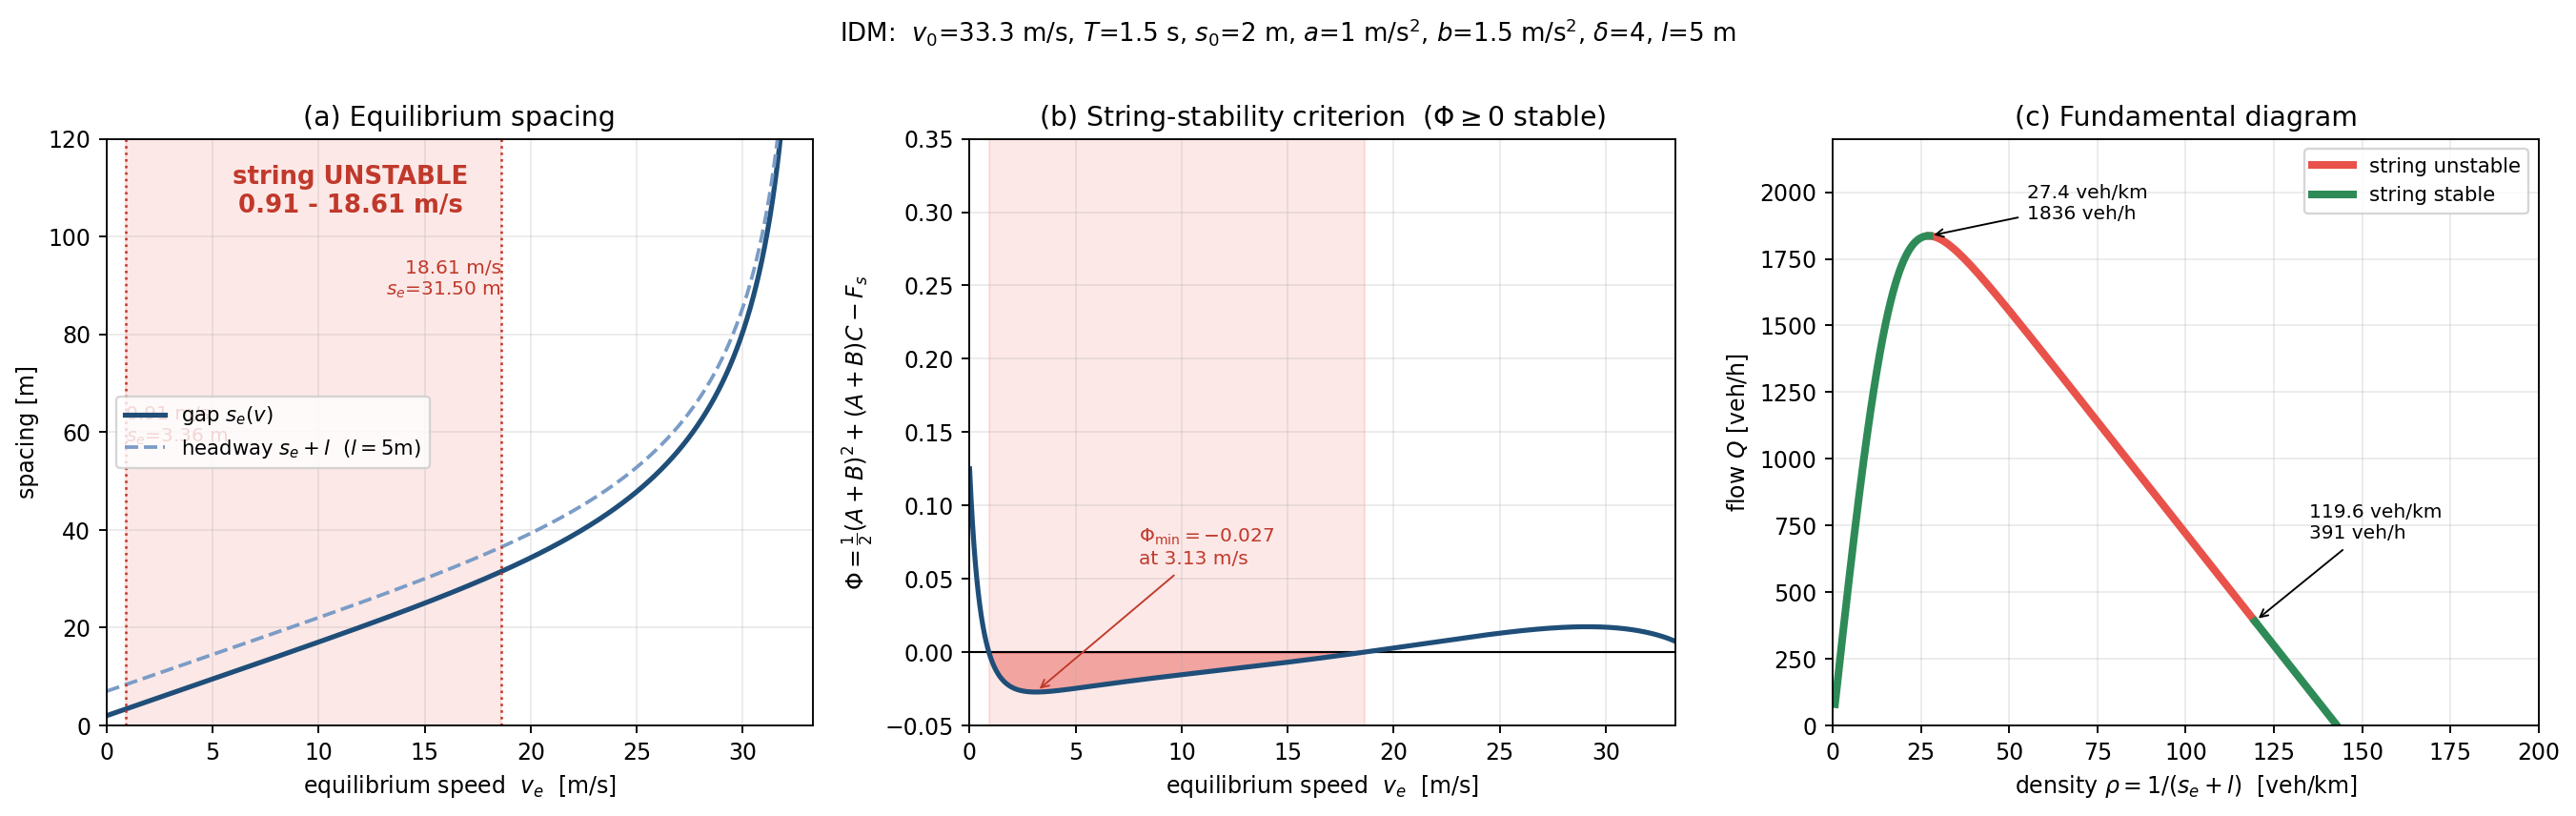
\includegraphics[width=\textwidth]{fig1.png}
\caption{Equilibrium states, stability criteria, and basic diagrams of the original IDM.}
\label{fig:idm-stability-map}
\figurenote{A one-to-one mapping between the equilibrium branches and stability regions of the reference IDM. The left figure shows the equilibrium net spacing corresponding to the velocity calculated using $F(s_e,v_e,0)=0$, indicating that while scanning $v_e$, density is also being scanned; the middle figure calculates the long-wave margin using $\Phi(v_e)$, where the two points where the curve crosses the zero line define the upper and lower boundaries of the instability zone—the region above the zero line is stable, and the region below is unstable. The right figure uses $\rho_e=1/(s_e+l)$ and $q_e=\rho_ev_e$ to project the same operating point onto the basic diagram; therefore, the red segments are not empirically colored but represent the image of the negative margin region from the middle figure in the flow–density coordinate system. A combined analysis of the three figures reveals that two operating points with similar flow rates may lie on different stable branches, indicating that knowing only the flow rate on the basic diagram is insufficient to determine whether a disturbance will grow or decay. This figure demonstrates that stability is a dynamic property attached to the equilibrium branch; the basic diagram defines “where the steady state is,” while the partial derivatives and dispersion relations define “where the system goes after departing from the steady state.”}
\end{figure}










A few points worth noting:










\begin{itemize}[leftmargin=1.4em,itemsep=3pt]
\item \textbf{The train length $l$ is not included in the stability criteria.} It affects only the horizontal axis of the base plot via $\rho = 1/(s_e+l)$; therefore, the density of unstable sections in the plot and the flow location depend on $l$, but the critical velocities of 0.91 and 18.61 m/s are independent of $l$.







\item \textbf{Low-speed, dense traffic is most prone to instability}




($v_e\approx3$ m/s), rather than the capacity point.







\item




The upper critical point lies just slightly to the right of the base-case capacity point (27.4 veh/km, 1,836 veh/h), meaning that under this set of parameters,




\textbf{the system becomes unstable near the capacity threshold}




, and disturbances amplify upstream into stop-and-go waves. This is precisely why IDM is often used to reproduce stop-and-go phenomena.







\item




At $v_e\to0$, $\Phi\to 0.125>0$ (due to $aT^2/s_0 = 1.125>1$), so the system is actually stable near complete standstill, and the unstable region has a lower boundary. If $T$ is reduced to below $1.41$ s, this lower boundary disappears, and the unstable region extends all the way to $v_e=0$.







\item




Local stability is always satisfied across the entire speed range; however, within the instability band at $f_v^2<4F_s$ (underdamped), the vehicle’s response itself is an oscillation that decays over time.


\end{itemize}

\section{Numerical Validation E1–E3: Neutral Line, Growth Rate, and Dominant Mode}
\sectionstudy{experiment}{Numerical Validation E1–E3: Neutral Line, Growth Rate, and Dominant Mode}{treiber2000,sugiyama2008,treiberkesting2013}
\label{sub:baseexp}

\begin{tcolorbox}[experimentbox,title=\textbf{Experimental Setup}]

E1: Scan $\Phi(v_e)$ on $v_e\in(0,v_0)$ and refine the sign-change points using the bisection method. E2–E3: Set $N=120$, $v_e=8$ to m/s, $s_e=14.0234$ to m, and $L=N(s_e+l)=2.2828$ to km; Superimpose a single-velocity-mode disturbance with an amplitude of $2\times10^{-3}$ m/s on the uniform steady state. Solve the microscopic equations using the fourth-order Runge–Kutta method and integrate for 300 s at $\Delta t=0.02$ s; perform a linear window fit over the interval $60$–$220$ s

\[
\operatorname{Re}\lambda=\frac{\mathrm d}{\mathrm dt}\ln|A_m(t)|,
\qquad
\operatorname{Im}\lambda=\frac{\mathrm d}{\mathrm dt}\arg A_m(t).
\]

A spatial FFT is used to identify the dominant mode $m^*$. All fitting points are constrained to $|A_m|<0.05$ m/s to avoid nonlinear saturation contaminating the slope.







\end{tcolorbox}

\begin{center}
\small
\captionof{table}{Analytical predictions and numerical verification for E1–E3.}
\label{tab:e1e3-validation}
\begin{tabular}{p{2.0cm}p{3.6cm}p{3.6cm}p{3.2cm}}
\toprule
\textbf{Experiments} & \textbf{Analytical Predictions} & \textbf{Numerical Results} & \textbf{Consistency} \\
\midrule


E1 Neutral Line




& $0.91$--$18.61$ m/s &




 Scan the range of token numbers $0.91$--$18.61$ m/s




&




 Both boundaries are reproduced




\\[3pt]
E2 growth rate

& $\operatorname{Re}\lambda=0.00408566$ s$^{-1}$ &

$0.00408565$ s$^{-1}$ (321 points)

&

Relative error $3.7\times10^{-5}\%$
\\[3pt]
E2 frequency

& $|\operatorname{Im}\lambda|=0.12821997$ rad/s & $0.12821997$ rad/s &

Relative error $1.1\times10^{-6}\%$
\\[3pt]
E3 dominant mode

& $m^*=4$，$k^*=0.20944$ rad/veh &

FFT peak located at $m=4$

&

Completely consistent
\\
\bottomrule
\end{tabular}
\end{center}
\tabletext{tab:e1e3-validation}{

Analytical and microscopic simulation values for the neutral line, growth rate, angular frequency, and dominant mode. The simultaneous agreement of these four items demonstrates that the validation goes beyond merely reproducing "stable/unstable" labels; it also quantitatively reproduces the temporal and spatial scales of the perturbations.
}

\begin{tcolorbox}[resultbox,title=\textbf{Validation conclusion}]
The analytical growth rate not only indicates stability or instability but also quantitatively predicts the exponential slope of the perturbation envelope and the phase rotation speed in the microscopic simulation. E3 further confirms that a finite loop can only sample specific discrete modes; therefore, the wavelengths observed in the simulation should be compared against the discrete spectrum rather than the peak of the continuous spectrum.


\end{tcolorbox}

\section{Specific trajectory results: Stability and instability of the original IDM}
\sectionstudy{experiment}{Specific trajectory results: Stability and instability of the original IDM}{treiber2000,treiberkesting2013}



Figure ~\ref{fig:traj-s0} shows results using the same local deceleration pulse while varying only the equilibrium speed. In the stable case ($v_e=25$ m/s), where $\sigma_v(1800)/\sigma_v(0)=0.00336$ applies, the probe vehicle maintains a speed of $24.9991$–$25.0006$ m/s and a spacing of $54.8905$–$54.8996$ m; the perturbation band dissipates rapidly. In the unstable case ($v_e=8$ m/s), the ratio increases to $48.49$, and the final-stage growth rate is $+3.12\times10^{-3}$ s$^{-1}$; the probe vehicle's speed range widens to $5.24$–$11.28$ m/s, and the spacing range expands to $9.73$–$19.67$ m. The diagonal red and blue bands on the spatiotemporal trajectory become increasingly pronounced, directly illustrating the upstream propagation and amplification of the perturbation.\begin{figure}[htbp]
\centering
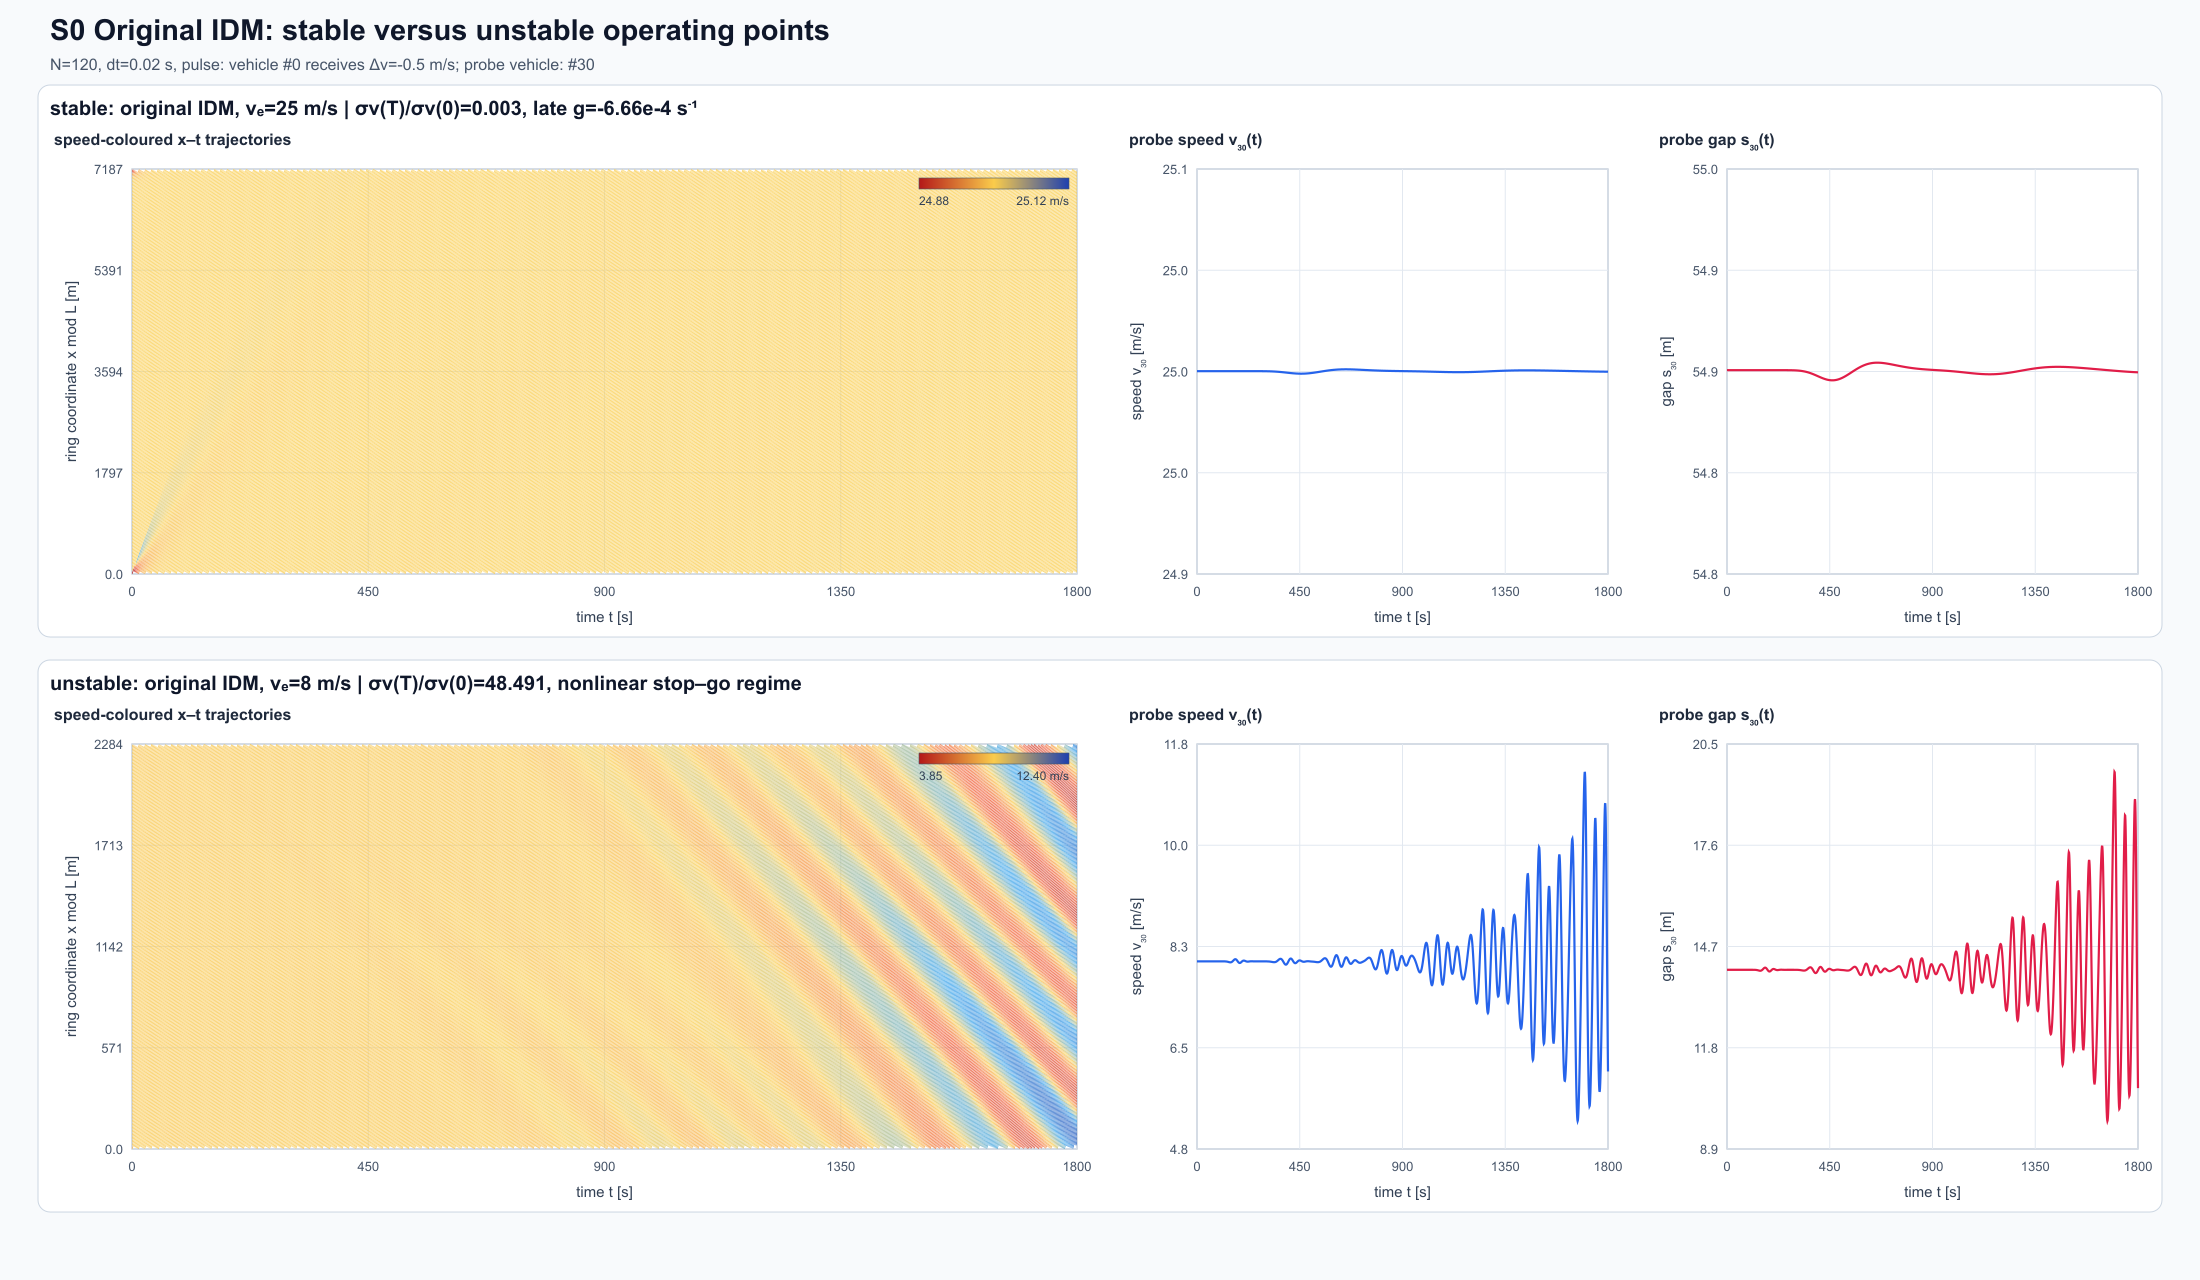
\includegraphics[width=\textwidth]{sim_s0_baseline.png}
\caption{S0: Stable and unstable trajectories of the original IDM.}
\label{fig:traj-s0}
\figurenote{A comprehensive time-domain comparison of the baseline IDM at stable and unstable operating points. Both scenarios utilize a time window of $N=120$ to $\Delta t=0.02$ s (duration: 1800 s) and apply an identical velocity pulse of $-0.5$ m/s to the lead vehicle (Vehicle 0); the only key difference is the parameter value—$v_e=25$ m/s for the upper case and $8$ m/s for the lower case. The left column displays actual road position-time trajectories, with vehicle colors indicating instantaneous velocity: in the upper case, the initial low-speed color band fades during propagation and reverts to a nearly uniform straight line, indicating that the perturbation is absorbed; in the lower case, the low- and high-speed bands intensify and widen with each cycle, forming periodic stop-and-go waves, which indicates that the small perturbation has entered a state of nonlinear saturation. The curves on the right, showing the velocity and net gap of the 30th vehicle, provide localized evidence: in the stable case, peaks and valleys converge synchronously, whereas in the unstable case, amplitudes continuously increase, with velocity minima corresponding to gap compression. Both visualizations provide consistent evidence regarding growth signs, propagation direction, and velocity-gap coupling; thus, the figure does not merely illustrate "congestion vs. no congestion" but directly validates the analytical criteria defined by $\Phi(25)>0$ and $\Phi(8)<0$.}
\end{figure}

\section{Instructional Example M03: Comparison of stable/unstable original IDM behavior under the same perturbation}
\sectionstudy{experiment}{Instructional Example M03: Comparison of stable/unstable original IDM behavior under the same perturbation}{treiber2000,treiberkesting2013}\label{sec:mini-examples}

M03 serves as the minimal dynamic verification case for the theoretical boundaries discussed in this chapter. It involves a trajectory shorter than 1800 s and excites only a single Fourier mode, allowing for a direct comparison between the analytical growth rate and the fitted slope; the remaining cases (M01, M02, and M04–M06) are addressed in the sections covering local stability, long-wave behavior, lead-vehicle acceleration, numerical convergence, and the LWR model, respectively.

We set $N=30$ and $m=1$, with an initial velocity mode amplitude of $0.002$ m/s and $\Delta t=0.05$ s, and integrate for 600 s. At $v_e=25$ m/s, the analytical rightmost root is $-0.0148584$ s$^{-1}$ and the simulation fit is $-0.0147203$ s$^{-1}$, with the final amplitude being only $8.92\times10^{-5}$ of the initial value; at $v_e=8$ m/s, the analytical value is $+0.00408566$ s$^{-1}$ and the simulation fit is $+0.00408551$ s$^{-1}$, with the amplitude amplifying to $5.26$ times the initial value after 600 s. Since only the equilibrium velocity differs between the two sets, the observed differences in the growth rate sign and mode envelope can be directly attributed to the stability region.



\begin{figure}[htbp]
\centering
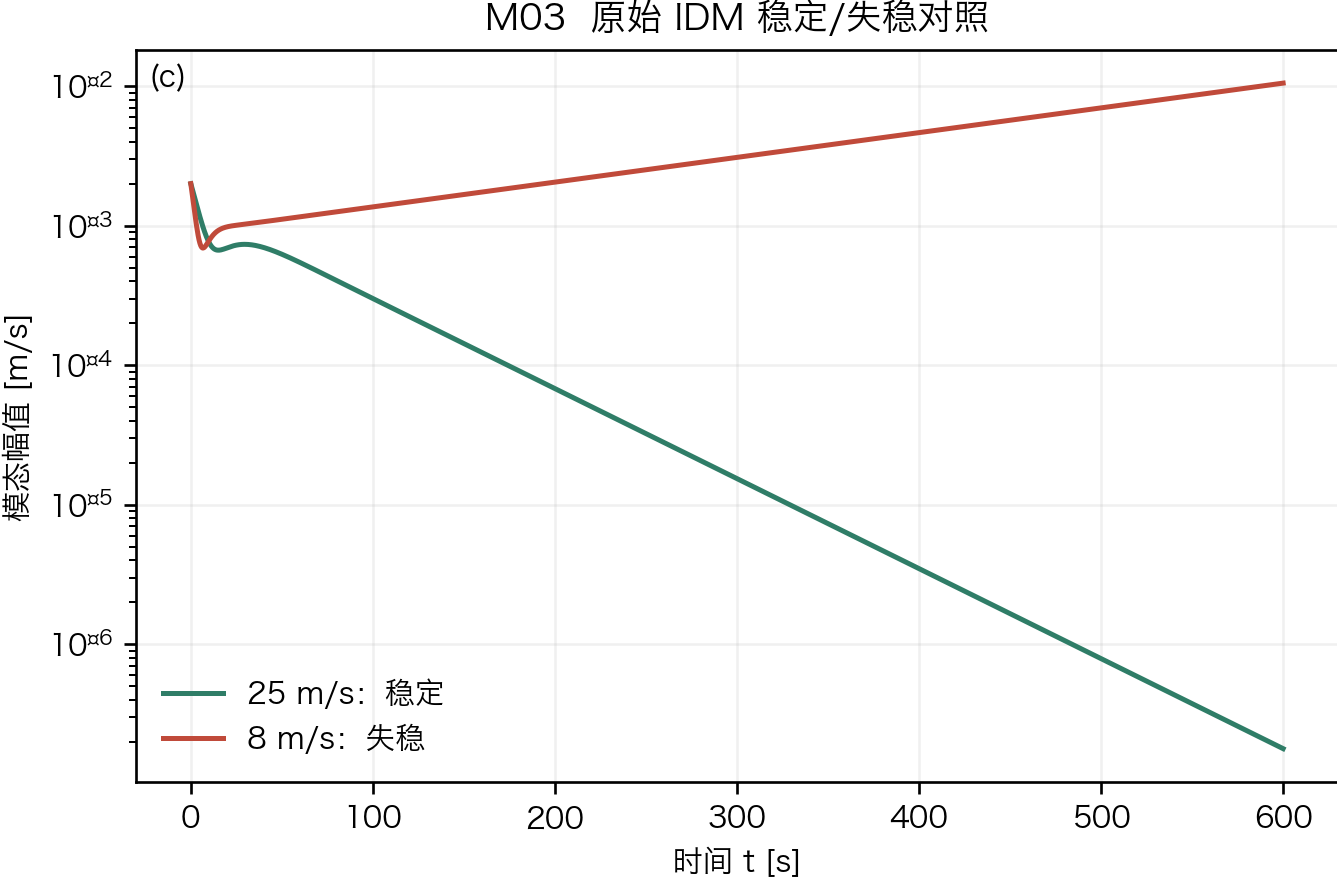
\includegraphics[width=0.86\textwidth]{mini_example_m03.png}
\caption{M03: Mode envelope of the original IDM.}
\label{fig:m03-baseline}
\figurenote{M03 extracts the envelope of the dominant velocity mode from the full nonlinear simulation shown in Fig. ~\ref{fig:traj-s0} and compares the analytical prediction with the fitted results on a logarithmic vertical axis. During the linear small-perturbation phase, if $A(t)\approx A_0e^{\sigma t}$ holds, then $\log A(t)$ should appear as a straight line with slope $\sigma$; in the figure, the curves slope downward for stable conditions and upward for unstable conditions, corresponding to negative and positive growth rates, respectively. The fitted lines align closely with the $\max_k\operatorname{Re}\lambda(k)$ values calculated from the dispersion relation, demonstrating that the fading or intensifying color bands observed visually in the position-time plot are not illusions caused by the color scale, but rather quantifiable exponential decay or growth. At later stages, the instability curves deviate from linearity and approach saturation, signaling the breakdown of the linear assumption rather than an error in the theoretical growth rate calculation. This figure thus establishes a chain of evidence linking the analytical spectrum, numerical mode amplitudes, and nonlinear spatiotemporal plots.
}
\end{figure}

\begin{tcolorbox}[resultbox,title=\textbf{What questions do the small-scale case study and the 1800 s trajectory answer respectively?}]
M03 uses a single mode to answer whether the analytical growth rate can be reproduced digit-for-digit; the long-duration case study in Fig. ~\ref{fig:traj-s0} answers how a local pulse evolves into a genuine stop-and-go wave following mode competition. The former is suitable for verification, while the latter is suited for observing the complete evolution; neither can substitute for the other.


\end{tcolorbox}

%==================================================================
\sectionwrapup{The benchmark case study employs identical parameters, perturbations, and an 1800 s time window to validate the analytical conclusions: at $v_e=25$ m/s, the color variations in the position-time trajectory and the oscillations in the velocity/spacing of a specific vehicle decay; at $v_e=8$ m/s, the perturbation grows into an upstream-propagating stop-and-go wave. Furthermore, M03's minimal single-mode experiment reduces the discrepancy between theoretical and fitted growth rates to a magnitude that allows for direct verification.}

\PART{II}{Analysis Map: From Single Factors to Combinations}

%==================================================================
\chapter{Quick Reference for Six Single Factors}
\label{sec:map}
\chapterguide{Which Stability Tool to Use When Adding a New Mechanism}{

Instead of repeating lengthy derivations, this chapter compares how feed-forward, look-back, multi-vehicle, delay, and heterogeneity mechanisms each disrupt specific structural properties. Readers can use this to determine whether to employ transfer functions, loop spectra, the Bilharz criterion, delay root-finding, or full-system eigenvalues.
}

Before diving into the step-by-step derivations, let us lay out all the factors. The effect of each factor

\textbf{in isolation}

when added to the baseline IDM from Chapter ~\ref{sec:num}~ is as follows; for combined scenarios, see

\S\ref{sub:layers}。

\section{Summary Table of Factors}
\sectionstudy{synthesis}{Summary Table of Factors}{wilsonward2011,feng2019}

\begin{center}
\scriptsize
\captionof{table}{Impact of six extended factors on model structure and stability criteria.}
\label{tab:six-factor-map}
\begin{tabular}{p{1.35cm}p{1.7cm}p{2.35cm}p{4.35cm}p{2.4cm}p{1.0cm}}
\toprule
\textbf{Factor} & \textbf{Notation} & \textbf{Disrupted Structure} & \textbf{Criterion for Isolated Effect} & \textbf{IDM Figure} & \textbf{See Details} \\
\midrule

F1 Lead vehicle acceleration

& $f_a$ &

Transfer function numerator and denominator have the same order&$\left|f_a\right|\le1$ and $\dfrac{f_v^2-f_{v_l}^2}{2}\ge\left(1-f_a\right)f_s$

& $\kappa_c=0.134$ &

Chapter ~\ref{sec:lead}~
\\[8pt]
F3 Acceleration of the following vehicle

& $f_b$ & \textbf{Unidirectional cascade} &

$\left|f_b\right|<1$; long-wave behavior same as above ($f_a\!\to\!f_b$), plus internal verification of $\widetilde W>0$

&

Positive sign window $0.134$–$0.43$; negative sign alone is detrimental

&

Chapter ~\ref{sec:bilat}~
\\[12pt]
F3 Multiple preceding/following vehicles

& $\alpha,\beta$ &

—($P$ becomes complex)

&

Long-wave behavior determined solely by $\sigma_{\rm eff}=\dfrac{f_a}{1-\alpha}+\dfrac{f_b}{1-\beta}$

&

When $\alpha=0.8$, $f_a=0.027$ suffices; $\beta\lesssim0.58$

&

Chapter ~\ref{sec:multi}~
\\[12pt]
F4 Backward spacing& $h_s,h_v$ &Unidirectional cascading,

\textbf{and changing wave speed} & $c_1=\left(1-h_s/f_s\right)V'$；$\dfrac{2(f_s+\mu f_{v_l})}{\mu^2}\le\dfrac{1+p}{(1-p)^2}$ & $p_c=0.223$ &

Chapter ~\ref{sec:reargap}~
\\[10pt]
F5 Time delay

& $\tau_0,\tau_a$ & \textbf{Polynomial nature} &

Long wave

\textbf{Completely invariant}

; addition of $\tau_0<\tau_0^{\rm crit}$ and $\Psi(\omega)\ge0$

& $\tau_0^{\rm crit}=1.16$--$2.52$ s &

Chapter ~\ref{sec:delay}~
\\[8pt]
F6 Platoon heterogeneity

& $F_n\ne F_{n-1}$ & \textbf{Translation invariance} &

Prefix sum $\sum_{n\le j}\eta_n\ge0$, weight $1/f_s^2$

&

Ring-road total budget threshold $26.7\%$

&

Chapter ~\ref{sec:het}~
\\
\bottomrule
\end{tabular}
\end{center}
\tabletext{tab:six-factor-map}{

Mathematical structures disrupted by lead/following vehicle acceleration, multi-vehicle information, backward spacing, delay, and heterogeneity, respectively. This table serves as an index for subsequent chapters: first identify where the structure is disrupted, then select the transfer function, ring-road spectrum, Bilharz criterion, or delay numerical method.
}

\section{Six conclusion cards}
\sectionstudy{theory}{Six Conclusion Cards}{wilsonward2011,feng2019}

\begin{tcolorbox}[keybox,title=\textbf{F1 Acceleration feedback from the leading vehicle (the only "pure gain" factor)}]
The only factor

\textbf{that neither disrupts the cascade nor alters the wave speed.}

It merely lowers the right-hand side of the long-wave condition from $f_s$ to $(1-f_a)f_s$, at the cost of introducing a high-frequency condition $\left|f_a\right|\le1$ that is invisible in the long-wave expansion (because $\left|G(i\infty)\right|=\left|f_a\right|$). Local stability remains completely unaffected.


\end{tcolorbox}

\begin{tcolorbox}[keybox,title=\textbf{F2 Acceleration feedback from the following vehicle (first instance of cascade disruption)}]
$y_n$ begins to depend on $y_{n+1}$; the concept of "vehicle-by-vehicle amplification factor" itself becomes invalid, necessitating a switch to the Routh-Hurwitz criterion with complex coefficients based on the cyclic eigenvalue $+$. At the long-wave scale, it is entirely equivalent to F1 (considering only the total sum); the differences lie solely in the phase terms associated with finite wavelengths.

\textbf{A positive sign is usable, though the window is only one-third that of the forward-looking case; using a negative sign in isolation actually worsens performance}

(by reducing the total magnitude); it must be paired with forward-looking feedback.


\end{tcolorbox}

\begin{tcolorbox}[keybox,title=\textbf{F3 Multi-vehicle feedback (diluting the gain)}]
The exponentially decaying kernel sums to a closed-form expression, where $1/(1-\alpha)$ represents the average observation distance. The long-wave threshold

\textbf{depends solely on the total magnitude}$\sigma_{\rm eff}$ is determined; thus, distributing the same total gain among multiple preceding vehicles allows the nearest-neighbor gain to be reduced according to $(1-\alpha)$. However, the spatial distribution still exhibits

\textbf{directional asymmetry}

: forward distribution does not reduce the long-wave margin, whereas backward distribution exacerbates the adverse contribution of the first moment.


\end{tcolorbox}

\begin{tcolorbox}[keybox,title=\textbf{F4 Backward spacing feedback (the only factor capable of altering wave speed)}]
Like F2, it disrupts the cascade effect, but it acts on $Q,R$ rather than $P$; therefore,

\textbf{it can directly reduce the kinematic wave speed}

and results in $c_1\to0$ in the fully symmetric limit. The right-hand side of the stability criterion is relaxed according to $(1-p)^{-2}$, indicating that it possesses the capability to adjust both the stability margin and the wave speed; this differs from feedback mechanisms that merely alter the acceleration kernel $P$.

\textbf{The "look-back effect" cited in the literature generally refers to this type of spacing/relative-velocity feedback, rather than the follower-vehicle acceleration feedback found in F2.}
\end{tcolorbox}

\begin{tcolorbox}[keybox,title=\textbf{F5 Time delay (only problematic at specific frequencies)}]
The characteristic equation becomes a quasi-polynomial, rendering the finite-dimensional Routh-Hurwitz and Bilharz criteria inapplicable. However,

\textbf{the long-wave condition remains unchanged.}: When $k\to0$ holds, $\lambda\to0$ and $e^{-\lambda\tau}\to1$ are satisfied. The impact of delay manifests in two ways: first, it introduces an upper bound on reaction lag for local stability; second, it may cause $\Psi(\omega)$ to drop below zero at finite frequencies.


\end{tcolorbox}

\begin{tcolorbox}[keybox,title=\textbf{F6 Heterogeneous platoon (Fourier failure, transfer function revival)}]
The matrix is no longer circulant; spatial Fourier analysis

\textbf{is completely inapplicable}

; however, the unidirectional cascade remains, making the chain product of

\textbf{vehicle-to-vehicle transfer functions}

the only effective tool—exactly the opposite of F2/F4. The long-wave condition transforms into a weighted prefix sum, where the weight $1/f_s^2$ causes "sluggish" vehicles to have a significant impact.


\end{tcolorbox}

\section{Complexity levels and tool selection}
\sectionstudy{synthesis}{Complexity levels and tool selection}{wilsonward2011,feng2019}
\label{sub:layers}

\begin{center}
\small
\captionof{table}{L0–L5 complexity levels and available analytical tools.}
\label{tab:complexity-levels}
\begin{tabular}{p{1.0cm}p{4.0cm}p{3.4cm}p{4.8cm}}
\toprule
\textbf{Level} & \textbf{Factors included} & \textbf{Characteristic equation type} & \textbf{Available tools} \\
\midrule
L0 &

Baseline (unidirectional, homogeneous, no delay)

&

Quadratic, real structure&Long-wave expansion $=$ transfer function
\\[4pt]
L1 &

$+$ F1, F3 (forward only)

&

Second-order, complex coefficients, cascaded (continuous)

& \textbf{Transfer function}

(Long-wave approximation insufficient; full frequency range required)
\\[4pt]
L2 &

$+$ F2 or F4

&

Second-order, complex coefficients, cascaded (discontinuous)

& \textbf{Cyclic eigenvalues $+$ Bilharz} \\[4pt]
L3 & $+$ F5 & \textbf{Quasi-polynomial} &

Long-wave closed-form $+$ Full-range numerical (D-partition / pseudospectral)
\\[4pt]
L4 & $+$ F6 &

Varies by vehicle

& \textbf{Chain product of vehicle transfer functions}

; Fourier method fails
\\[4pt]
L5 &

Combination (see below)

&

Depends on the combination

&

Both simplification types may fail simultaneously $\Rightarrow$ Direct calculation $2N$ Eigenvalues\\
\bottomrule
\end{tabular}
\end{center}
\tabletext{tab:complexity-levels}{A hierarchy of complexity ranging from the uniform, unidirectional, delay-free case to heterogeneous composite models. Uniformity determines the applicability of Fourier analysis, while unidirectionality determines whether scalar transfer functions can be used; when both properties are absent, the full state matrix must be solved.
}

\begin{tcolorbox}[notebox,title=\textbf{A decision rule}]
\[
\text{homogeneity} \;\Longrightarrow\; \text{spatial Fourier analysis is available},
\qquad
\text{unidirectionality} \;\Longrightarrow\; \text{a transfer function is available}
\]



If one of each is missing, one type of tool is lost; if both are missing (heterogeneous $+$ bidirectional), only the $2N$ eigenvalues can be calculated directly.







\end{tcolorbox}

\section{Combinations Covered in This Book}
\sectionstudy{theory}{Combinations Covered in This Book}{wilsonward2011,feng2019}

\begin{center}
\small
\captionof{table}{Factor combinations emphasized in this book.}
\label{tab:factor-combinations}
\begin{tabular}{p{3.8cm}p{2.0cm}p{7.4cm}}
\toprule
\textbf{Combinations} & \textbf{Layers} & \textbf{New conclusions} \\
\midrule







F1 $+$ F2 (bidirectional)




& L2 &




Long waves are determined solely by $\sigma=f_a+f_b$; asymmetry takes effect starting from $O(\varepsilon^3)$ and controls the finite-wavelength branch (Chapter ~\ref{sec:bilat}~)




\\[6pt]
F3 Bidirectional (exponential kernel)

& L2 &

Unified framework: arbitrary kernels compressed into $P(k)$; zeroth-order moment governs long waves, first-order moment governs finite wavelengths (Chapter \ref{sec:multi})
\\[6pt]
F1 $+$ F5 & L3 &

Long-wave threshold remains unchanged, while the upper bound of gain is suppressed; at $\tau_a\approx\tau_0$, the two effects partially cancel out (Chapter \ref{sec:delay})
\\[6pt]
F2 $+$ F5 & L3 &

Neither scalar transfer functions nor finite-dimensional Bilharz closed-form solutions apply; a combination of long-wave closed-form solutions and numerical eigenvalues is required
\\[6pt]
F6 $+$ F1 (mixed traffic)

& L4 &

Feed-forward capability depends on

\textbf{the type of the leading vehicle}

; $\eta_n$ depends on adjacent pairs, and even the aggregate sum depends on the ordering (

\S\ref{sub:mixed}） \\
\bottomrule
\end{tabular}
\end{center}
\tabletext{tab:factor-combinations}{

Representative combinations of bidirectionality, multi-vehicle interactions, delays, and mixed traffic, along with new conclusions. This demonstrates that composite models are not merely simple superpositions of single-factor findings; specifically, heterogeneity combined with bidirectional coupling, or feed-forward dynamics combined with communication delays, can alter the mathematical tools available for analysis.}

%==================================================================
\sectionwrapup{The six categories of factors can be classified based on whether they alter the unidirectional cascade, polynomial structure, or vehicle homogeneity. This mapping determines whether to employ transfer functions, ring-road dispersion relations, complex coefficient criteria, delay spectra, or full-platoon matrices, thereby avoiding the mechanical application of inapplicable closed-form formulas.}

\chapter{Protocol for Reproducible Numerical Experiments}
\label{sec:protocol}
\chapterguide{Making "Theory-Simulation Consistency" a Verifiable Conclusion}{

This chapter standardizes initial conditions, perturbations, time windows, numerical step sizes, output metrics, and convergence checks, while defining verification tasks E1 through E14. It serves both as an operational specification for the experimental testbed and as a prerequisite for ensuring the comparability of all figures and tables throughout the book.
}

This chapter consolidates the numerical examples scattered throughout the text into a unified set of reproducible experiments. The accompanying testbed features eight stackable scenarios: S0 (Baseline IDM), S1 (Lead Vehicle Acceleration), S2 (Following Vehicle Acceleration), S3 (Multiple Lead/Following Vehicles), S4 (Backward Spacing), S5 (Time Delay), S6 (Vehicle Heterogeneity), and S7 (Mixed AV/HDV). The interface is organized into "Real-time Ring Road," "Propagation \& Probes," "Theory \& Verification," and "Model Settings," decoupling animation observation, parameter control, and quantitative assessment. Each experiment reports both

\textbf{analytical predictions}

and

\textbf{actual simulation measurements}

rather than relying solely on animations to judge stability.

\section{Standardizing Initial Conditions, Perturbations, and Numerical Formats}
\sectionstudy{numerical}{Standardizing Initial Conditions, Perturbations, and Numerical Formats}{sugiyama2008,treiberkesting2013}Unless otherwise specified in the experiments, the IDM parameters from Chapter ~\ref{sec:num}~, $N=120$, and $\Delta t=0.02$ s are used. Given the density or loop length, the common equilibrium velocity is determined first; homogeneous traffic flow satisfies $s_e=L/N-l$, while heterogeneous traffic flow satisfies
\[
\sum_{n=1}^{N}\left[s_e^{(n)}(v_e)+l_n\right]=L,
\]





Thus ensuring




\textbf{Same speed, different distances}The true steady state. The default perturbation is a single-vehicle speed pulse or a single Fourier mode, with an amplitude not exceeding $2\times10^{-3}$--$5\times10^{-2}$ m/s.










\begin{tcolorbox}[experimentbox,title=\textbf{Numerical Implementation Conventions}]
\begin{enumerate}[leftmargin=1.6em,itemsep=3pt]
\item




Use the fourth-order Runge–Kutta method for the delay-free reference; semi-implicit updates may be used for interactive animations, but quantitative tables must be verified using RK4.







\item




 The acceleration coupling for S2/S3 is defined in $(I-K)\bm a=\bm a_{\rm IDM}$. At each step, solve the strip-linear system or iterate at a fixed point to $\|\bm a^{(r+1)}-\bm a^{(r)}\|_\infty<10^{-9}$; do not directly substitute the acceleration from the previous step.







\item




 S5 performs linear interpolation on $t-\tau$ using a circular history buffer; the history segment is initialized to a uniform equilibrium state.







\item




Each quantitative experiment is rerun using $\Delta t$ and $\Delta t/2$. If the growth rate, critical point, or wave velocity deviates beyond the limits specified in $1\%$, the result is rejected.







\item




Report the fitting time window, number of samples, and perturbation amplitude; stop the exponential fitting immediately after the perturbation enters nonlinear saturation.







\end{enumerate}
\end{tcolorbox}

\section{Tutorial Example M05: How to Distinguish Between Traffic Instability and Numerical Instability}
\sectionstudy{experiment}{Tutorial Example M05: How to Distinguish Between Traffic Instability and Numerical Instability}{sugiyama2008,treiberkesting2013}


\label{sub:m05-convergence}




For the instability conditions of M03, use RK4 to take $\Delta t=0.4,0.2,0.1$ s, and reduce the initial amplitude

reduced to $2\times10^{-4}$ m/s, and the growth rate was fitted over the interval $150$–$550$ s. The results of the third-order analysis are

\[
0.0040856540,\qquad 0.0040856554,\qquad 0.0040856555\ {\rm s}^{-1},
\]

The analytical value is $0.0040856555$ s$^{-1}$. The corresponding relative errors are, in order,

$3.78\times10^{-5}\%$, $3.43\times10^{-6}\%$, and

$1.53\times10^{-6}\%$.










\begin{figure}[htbp]
\centering
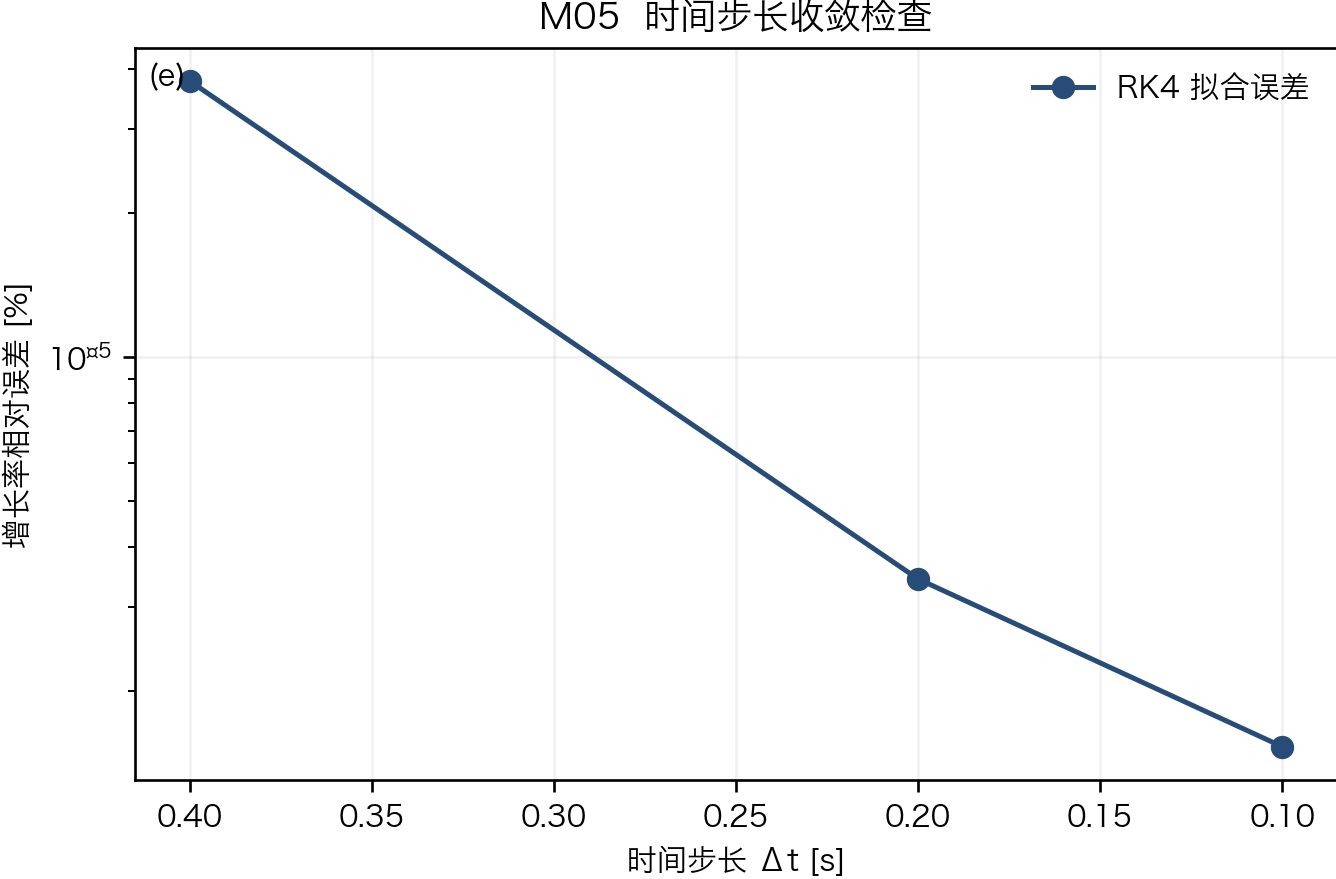
\includegraphics[width=0.82\textwidth]{mini_example_m05.png}
\caption{M05: Time-step convergence check.}
\label{fig:m05-convergence}
\figurenote{M05 performs a grid convergence check on the time-discretization error. Using the same model, initial conditions, number of vehicles, and fitting window, only the RK4 step size is varied; the dominant growth rate is recalculated at each point, with the finest step size or the analytical spectrum serving as the reference. As $\Delta t$ decreases, the points converge toward a stable limit, and $\Delta t=0.02$s have settled into a plateau region with minimal variation, indicating that the growth signs and dominant timescales shown in subsequent figures do not depend on any particular random time step. If a point with a coarse step size crosses the zero line, numerical damping may be misinterpreted as stability, or discrete oscillations may be misinterpreted as instability; this figure explicitly rules out such risks. It is therefore not merely an incidental program test, but a reliable prerequisite for all time-domain validations, and provides the basis for balancing accuracy against the computational cost of a 1,800-second simulation.}
\end{figure}










The comparison required here is




\textbf{the convergence of the same physical quantity}, rather than comparing whether the two animations are similar.

If, after halving the step size, the growth rate changes sign, the critical speed shifts significantly, or a negative spacing appears, then the original results cannot be used to verify stability.

Conversely, the fact that the positive growth rate in M05 is maintained to at least seven significant digits across three step sizes indicates that the growth stems from the IDM

physical branch rather than the RK4 discretization error.










\section{Unified Method for Plotting Spatio-Temporal Trajectories and Probe Car Curves}
\sectionstudy{experiment}{Unified Method for Plotting Spatio-Temporal Trajectories and Probe Car Curves}{sugiyama2008,treiber2000,treiberkesting2013}










In addition to the aforementioned small-perturbation fitting experiments, the following sections also provide a set of




\textbf{Long-time-domain trajectory examples where perturbation propagation can be directly observed}




. $N=120$ and $\Delta t=0.02$ s are uniformly adopted, and the observation window is set to $0\le t\le1800$ s; At $t=0$, the 0th vehicle generates a local deceleration pulse of $\Delta v_0=-0.5$ m/s, and the 30th vehicle is fixed for observation.




The left column of each set of figures shows the actual $x$–$t$




\textbf{Vehicle Spatio-Temporal Trajectories}




: The vertical axis represents the circuit coordinates $x\bmod L$; each thin line represents a vehicle’s trajectory, with the line color indicating the instantaneous speed at that moment (red/orange indicates slower speeds, blue indicates faster speeds). The trajectory breaks when it crosses $x=L$ and reappears at $x=0$. The right side only displays\textbf{A designated probe vehicle}




with $v_{30}(t)$ and $s_{30}(t)$, rather than stacking the time series of all vehicles together.




$\sigma_v(1800)/\sigma_v(0)$ in the figure caption is the ratio of the initial to final standard deviation of the vehicle’s speed; during the linear phase, the slope of the final segment’s envelope, $g=\mathrm d\ln\sigma_v/\mathrm dt$, is reported separately. If the disturbance has entered a finite-amplitude stop-and-go wave, only the ratio of initial to final values and the trajectory shape are used as nonlinear results; $g$ from the final segment is no longer used to explain the linear growth rate.










\section{Online Intervention Experiment: Comparing Before and After Control on the Same Trajectory}
\sectionstudy{experiment}{Online Intervention Experiment: Comparing Before and After Control on the Same Trajectory}{milanes2014,stern2018}










Static parameter sweeps answer the question of “whether a set of fixed parameters is stable,” but engineering control must also address another question:




\textbf{Can an established stop-and-go wave be gradually eliminated without disrupting traffic flow?}




 To this end, the test bench allows the acceleration feedforward gain of the lead vehicle, the acceleration gain of the trailing vehicle, the multi-vehicle weighting, and the rear-to-front distance weighting to be modified after the simulation begins; the vehicles’ positions, speeds, history buffers, and recorded images are all retained and not reinitialized.




To prevent sudden parameter changes from triggering high-frequency responses, a linear ramp is used for the lead vehicle’s acceleration feedforward: if the gain is adjusted from $\kappa_-$ to $\kappa_+$ at $t=t_{\rm int}$, with a transition time of $T_r$, then

The gain is ramped continuously from the pre-intervention value to the target value during the transition interval.


The velocity-spacing space-time plot records $t_{\rm int}$ using markers, allowing for a direct comparison within the same plot of the pre-intervention growth of fluctuations, the transition phase, and the post-intervention decay.




The built-in “Congestion Formation $\rightarrow$ Controlled Dissipation” example uses $N=60$, $\rho=50$ veh/km, $\Delta t=0.02$ s, using the benchmark IDM parameters from this book, and sets the 0th vehicle to generate a braking pulse of $-2.5$ m/s. The system first evolves using the original IDM ($\kappa=0$), and at $t_{\rm int}=600$ s, $\kappa$ is smoothly increased to $0.45$ over $T_r=120$ s. During a complete platform review, the standard deviation of velocity reached $0.534$ m/s at $t\approx543$ s, forming a visible run-and-stop wave; after intervention, it dropped to $0.018$ m/s at $t\approx974$ s, and the loop once again approached steady flow. This example demonstrates that the controller can dissipate nonlinear fluctuations that have already formed, but it




\textbf{does not replace}




the measurements of critical gain for small perturbations and linear growth rates in E1–E4.










\begin{tcolorbox}[experimentbox,title=\textbf{Sequence for Interpreting Online Interventions}]

First, use the loop animation to confirm that a traffic congestion wave has formed; then, on the speed-and-interval spatiotemporal map, compare the width and propagation direction of the color bands on either side of the intervention line; next, check whether the $v_n(t)$ and $s_n(t)$ values for the designated probe vehicle have returned from periodic, large-amplitude oscillations to narrow-amplitude fluctuations; Finally, use the decay of $\sigma_v(t)$ and $\sigma_s(t)$ to confirm that the improvement is not a localized or short-term phenomenon. If you need to estimate the stability boundary, you should return to the small-amplitude Fourier perturbation and fixed-parameter experiments.







\end{tcolorbox}

\section{Measured Quantities and Evaluation Criteria}
\sectionstudy{theory}{Measured Quantities and Evaluation Criteria}{sugiyama2008,treiberkesting2013}

\begin{center}
\small
\captionof{table}{Key measured quantities in stability experiments and their analytical counterparts.}
\label{tab:experiment-observables}
\begin{tabular}{p{2.0cm}p{4.2cm}p{7.0cm}}
\toprule
\textbf{Quantities} & \textbf{Numerical Measurement Methods} & \textbf{Correspondence with Analytical Quantities} \\
\midrule







Growth Rate




&




Least-squares linear fit to $\ln|A_m(t)|$




&




Slope compared to $\max_m\operatorname{Re}\lambda_m$\\[3pt]

Leitwellenzahl




&






Perform spatial FFT for $v_n-\bar v$






&Comparison of peak values ​​of $m$ and $\arg\max_m\operatorname{Re}\lambda_m$





\\[3pt]

Wellengeschwindigkeit




&




Anpassung an $\mathrm d\arg A_m/\mathrm dt$ nach Phasenentfaltung der dominanten Moden




&






$c_1=-\operatorname{Im}\lambda/k$; the slope of the space-time diagram serves only as an auxiliary value





\\

[3pt]

Transmission ratio






&






In the open platoon, the leading vehicle is subjected to a small sinusoidal perturbation; the amplitude ratio is determined after the steady state is reached






&






Comparison with $|G(i\omega)|$ or the product of the individual cars





\\[3pt]

Zwischenwert




&






Calculation of $\max_j|Y_j/Y_0|$ along the sequence of cars

& Comparison with $\max_j\prod_{n\le j}|G_n|$



\\
\bottomrule
\end{tabular}
\end{center}
\tabletext{tab:experiment-observables}{




Numerical methods for measuring the growth rate, dominant wavenumber, wave velocity, inter-wave transmission ratio, and prefix peak. Each quantity corresponds to a different analytical object; therefore, stability cannot be determined based solely on the color in the animation.
}

\section{Correspondence between E1–E14 and Chapters}
\sectionstudy{experiment}{Correspondence between E1–E14 and Chapters}{sugiyama2008,treiberkesting2013}

\begin{center}
\scriptsize
\captionof{table}{E1–E14: Experiments, Procedures, and Corresponding Chapters.}
\label{tab:experiment-index}
\begin{tabular}{p{0.85cm}p{2.3cm}p{3.5cm}p{4.2cm}p{2.7cm}}
\toprule
& \textbf{Experiments} & \textbf{Procedures} & \textbf{Core Controls} & \textbf{Corresponding Chapters} \\
\midrule
E1 &




 Neutral Stability Line




&




 Scan $v_e$ or IDM parameters and bisect the critical point




&




 Sign change of numerical growth rate vs. sign change of criterion function




&




Chapter ~\ref{sec:num}~



\\
E2 &




Growth Rate




&




Linear Window Fitting with Small Perturbations




&




 Measured $\operatorname{Re}\lambda$ vs. Ring Spectrum




& \S\ref{sub:baseexp} \\
E3 &




Most Unstable Wavenumber




&




Spatial FFT& Measured $m^*$ vs. Spectral Peak




&




 Chapter ~\ref{sec:bilat}~, Chapter ~\ref{sec:multi}~



\\
E4 &




 Vehicle-to-vehicle transmission ratio




&




 Open-loop sine sweep




& $|Y_n/Y_{n-1}|$ vs $|G(i\omega)|$ &




 Chapter ~\ref{sec:lead}~



\\
E5 &




 Limited $N$




&




 Scan $N=10$--$300$




&




 Critical band vs $\cos(2\pi/N)$




&




 Chapter ~\ref{sec:appx}~



\\
E6 &




 Ordering effect




&




 Fixed formula, changed order




&




 Midpoint Peak vs. Terminal Product




& \S\ref{sub:hetorder} \\
E7 &




 AV Permeability




&




 Scanned AV Fraction, Rate, and Number of Compartments




&




 Two-Dimensional Steady State, $p_{\min}$, $n_{\rm grp}^{\max}$




& \S\ref{sub:mixed} \\
E8 &




 Time delay& Scannen von $\tau_0,\tau_a$




&




 $\Psi(0)$ und $\min_\omega\Psi$




&




 Kapitel ~\ref{sec:delay}~



\\
E9 &






backward weight






&




Scan $p$




&






closing point of the instability band $p_c$






&




 Kapitel ~\ref{sec:reargap}~



\\
E10 &




 Wellengeschwindigkeit




&






phase alignment and spatiotemporal representations






& $c_1=(1-p)V'(s_e)$ &




 Kapitel ~\ref{sec:reargap}~



\\
E11 &




 Schwache nichtlineare Entwicklung




&






long-term integration of a small-amplitude sinusoidal perturbation






&






linear growth, waveform steepness, and saturation






& \S\ref{sub:nonlinear-exp} \\
E12 &






Recovery with limited amplitude






&






steady-state amplitude of the individual vehicle braking






&






Peak value, residual value at the end of the window, and recovery time






&




Kapitel ~\ref{sec:nonlinear}~



\\
E13 &






macro-stability

& Relaxed ARZ Stable/Instability Operating Points on the IDM Basic Diagram




&




 Dispersion Relations and Fixed-Point Velocity-Time Curves




& \S\ref{sub:macro-experiment} \\
E14 &




 Micro-Macro Consistency




&




Side-by-Side Simulation of the IDM Basic Diagram and ARZ with Long-Wavelength Closure




&




Similarity of Growth Rates, Wave Speeds, and Spatio-Temporal Velocity Maps




& \S\ref{sub:micro-macro-experiment} \\
\bottomrule
\end{tabular}
\end{center}
\tabletext{tab:experiment-index}{




Operations, theoretical comparisons, and main text locations for the fourteen sets of experiments. Readers can look up the corresponding derivations by experiment number or select the relevant experiments to reproduce based on the chapter.
}

\begin{tcolorbox}[notebox,title=\textbf{AV, HDV, and vehicle model heterogeneity are two distinct sets of labels}]

In S7, the HDV uses only IDM with a feedforward gain of $0$; the AV uses $\kappa$ when following another AV and a degraded gain of $\kappa_0$ when following the HDV. In S6, vehicle model and driving style parameters such as $v_0,T,a,b$ are modified. The two types of labels can be combined: a vehicle with conservative parameters can also be equipped with an autonomous driving controller. Unless S6 is explicitly enabled, the AV and HDV use exactly the same IDM parameters; therefore, the differences in S7 stem solely from information and control capabilities.







\end{tcolorbox}

\sectionwrapup{All scenarios use uniform initial equilibrium values, perturbation amplitudes, an 1800-second observation window, and convergence checks, while simultaneously outputting position-time velocity-colored trajectories, specified vehicle speed/spacing curves, and theoretical growth rates. AV/HDV labels indicate control capabilities, while vehicle model heterogeneity labels indicate differences in IDM parameters; the two must not be used interchangeably.}

\PART{III}{Maintaining Unidirectional Cascading: Lead Vehicle Acceleration Feedback}

\chapter{Generalization: Considering the Effect of Lead Vehicle Acceleration}
\label{sec:lead}
\chapterguide{Why Does Lead Vehicle Acceleration Feedforward Expand the Stability Region?}{




This chapter explains how pure feedforward does not alter the local root of a single vehicle but does change the numerator and high-frequency limit of the vehicle-to-vehicle transfer function. After reading this chapter, you should be able to calculate the critical gain while simultaneously verifying the long-wave gain, finite-frequency peak, and upper bound of the gain.
}

\section{Model Setup}
\sectionstudy{model}{Model Setup}{milanes2014,ploeg2014,feng2019}










Add lead-car acceleration feedback (the feedforward term in CACC) to the original model:

\begin{equation}
\dot v_n = F\left(s_n,\; v_n,\; \dv_n,\; \dot v_{n-1}\right)
\end{equation}




Convert to the equivalent form $\dot v_n = f(s_n,v_n,v_{n-1},\dot v_{n-1})$; the four partial derivatives at the equilibrium point are:

\begin{equation}
f_s>0,\qquad f_v<0,\qquad f_{v_l}>0,\qquad
f_a \equiv \frac{\partial f}{\partial \dot v_{n-1}}\ \ (\text{generally}\ \ge 0)
\end{equation}










\textbf{The steady-state remains unchanged.}




At steady state, $\dot v_{n-1}=0$; the new term automatically becomes zero, so $V(s_e)$ and $V'(s_e)$ are identical to those in the previous section.




Linearization:

\begin{equation}
\delta\dot s_n = \delta v_{n-1}-\delta v_n,
\qquad
\delta\dot v_n = f_s\,\delta s_n + f_v\,\delta v_n + f_{v_l}\,\delta v_{n-1} + f_a\,\delta\dot v_{n-1}
\end{equation}










\section{Local stability: Completely unchanged}
\sectionstudy{theory}{Local stability: Completely unchanged}{wilsonward2011,ororsz2010}










When the leading vehicle is traveling at a constant speed, $\delta v_{n-1}\equiv 0$ and $\delta \dot v_{n-1}\equiv 0$; new term




\textbf{The entire term vanishes}

, the characteristic equation remains

\begin{equation}
\lambda^2 - f_v\lambda + f_s = 0
\qquad\Longrightarrow\qquad
f_v<0,\quad f_s>0
\end{equation}












\begin{tcolorbox}[notebox]

The acceleration of the preceding vehicle is a purely feedforward component; it does not enter the closed-loop control system of the ego vehicle and has no influence whatsoever on the ego vehicle's response behavior. This also illustrates that:






\textbf{A local stability analysis alone reveals nothing about the benefit of adding this term.}






– Its effect manifests exclusively at the level of the vehicle platoon. \end{tcolorbox}

\section{Linear stability: Transfer function}
\sectionstudy{theory}{Linear stability: Transfer function}{swaroop1996,ploeg2014,feng2019}












With position disturbance:

\begin{equation}
\ddot y_n = f_s\left(y_{n-1}-y_n\right) + f_v\,\dot y_n + f_{v_l}\,\dot y_{n-1} + f_a\,\ddot y_{n-1}
\end{equation}




Following exactly the same steps as in Section 3.2, the Laplace transform is applied assuming zero initial conditions ($\mathcal{L}\{\ddot y_{n-1}\}=\lambda^2Y_{n-1}$):

\begin{equation}
\lambda^2 Y_n = f_s\left(Y_{n-1}-Y_n\right) + f_v\lambda Y_n + f_{v_l}\lambda Y_{n-1} + f_a\lambda^2 Y_{n-1}
\end{equation}




Separation of $Y_n$ and $Y_{n-1}$:

\begin{equation}
\left(\lambda^2 - f_v\lambda + f_s\right)Y_n = \left(f_a\lambda^2 + f_{v_l}\lambda + f_s\right)Y_{n-1}
\end{equation}












\begin{tcolorbox}[keybox]
\begin{equation}
G(\lambda) = \frac{\hat y_n}{\hat y_{n-1}}
= \frac{f_a\lambda^2 + f_{v_l}\lambda + f_s}{\lambda^2 - f_v\lambda + f_s}
\label{eq:Ga}
\end{equation}
\end{tcolorbox}












Compared to the formula ~\eqref{eq:G0}, the crucial change is that






\textbf{the term $\lambda^2$ is added to the numerator}






, such that

\begin{equation}
\lim_{\omega\to\infty}\left|G(i\omega)\right| = \left|f_a\right|
\end{equation}

no longer tends towards 0. This determines success or failure.












\section{Expansion of the condition}
\sectionstudy{theory}{Expansion of the condition}{milanes2014,ploeg2014,feng2019}


\label{sub:leadcond}




\begin{align}
\left|N(i\omega)\right|^2 &= \left(f_s - f_a\omega^2\right)^2 + f_{v_l}^2\omega^2 \\
\left|D(i\omega)\right|^2 &= \left(f_s - \omega^2\right)^2 + f_v^2\omega^2
\end{align}




Using the difference of squares:

\begin{equation}
\left(f_s-\omega^2\right)^2 - \left(f_s-f_a\omega^2\right)^2
= \left(f_a-1\right)\omega^2\left[2f_s-\left(1+f_a\right)\omega^2\right]
\end{equation}




Therefore,

\begin{equation}
\left|D\right|^2 - \left|N\right|^2
= \omega^2\Big\{\left(f_a-1\right)\left[2f_s-\left(1+f_a\right)\omega^2\right] + f_v^2 - f_{v_l}^2\Big\}
\end{equation}




Let $u = \omega^2 \ge 0$, and the expression inside the curly braces is simplified to $u$:




\textbf{Linear function}：
\begin{tcolorbox}[keybox]
\begin{equation}
H(u) = \left(1-f_a^2\right)u + \left[f_v^2 - f_{v_l}^2 - 2f_s\left(1-f_a\right)\right] \;\ge\; 0
\qquad \forall\, u\ge 0
\end{equation}
\end{tcolorbox}










A linear function is non-negative at $[0,\infty)$ if and only if its slope is non-negative and its y-intercept is non-negative:










\begin{tcolorbox}[keybox,title=\textbf{General stability conditions for a straight line (including the acceleration of the leading vehicle)}]
\begin{align}
\text{(i)}\quad & \left|f_a\right| \le 1 \\[4pt]
\text{(ii)}\quad & \frac{1}{2}\left(f_v^2 - f_{v_l}^2\right) \;\ge\; \left(1-f_a\right)f_s
\end{align}
\end{tcolorbox}










When $f_a=0$ holds, we return to equation ~\eqref{eq:string}, which is self-consistent. Expressed using the original partial derivatives ($f_a = F_{\dot v_l}$):

\begin{equation}
\frac{1}{2}F_v^2 + F_vF_{\dv} \;\ge\; \left(1-f_a\right)F_s
\end{equation}










\section{Why Is the Long-Wave Expansion Insufficient This Time?}
\sectionstudy{theory}{Why Is the Long-Wave Expansion Insufficient This Time?}{milanes2014,ploeg2014,feng2019}










Performing the same expansion as $\varepsilon=-ik\to0$, the dispersion relation becomes

\begin{equation}
\lambda^2\left(1-f_a e^{\varepsilon}\right) = f_s\left(e^{\varepsilon}-1\right) + \left(f_v+f_{v_l}e^{\varepsilon}\right)\lambda
\end{equation}




Step-by-step matching shows that $c_1 = V'(s_e)$ remains unchanged, while

\begin{equation}
c_2 = \frac{\left(1-f_a\right)c_1^2 - \frac12 f_s - f_{v_l}c_1}{f_v+f_{v_l}}
\end{equation}




requires $c_2\ge0$; after rearrangement,




\textbf{this precisely satisfies condition (ii), but fails to satisfy condition (i)}。

\begin{tcolorbox}[notebox,title=\textbf{Key Methodological Points}]

The reason lies in $\left|G(i\infty)\right| = \left|f_a\right|$: when $f_a>1$ occurs, the slope of $H(u)$ is negative, and instability first occurs in $\omega\to\infty$ (short waves); this is completely invisible in the long-wave expansion.










\textbf{Once the model includes the lead-car acceleration, or any term that causes the numerator and denominator of the transfer function to be of the same order, a complete frequency-domain analysis must be performed; relying solely on the long-wave expansion may omit high-frequency instability branches.}
\end{tcolorbox}

\section{Physical Interpretation}
\sectionstudy{theory}{Physical Interpretation}{milanes2014,ploeg2014,feng2019}

\textbf{Condition (i): The feedforward gain must not overshoot.}




 The acceleration of the lead vehicle is amplified and transmitted to the following vehicle, resulting in high-frequency $\left|G\right|\to f_a$. If $f_a>1$, this means that the jitter is amplified each time it is transmitted to the next vehicle, causing the entire convoy to disperse at high frequencies.










\textbf{Condition (ii): $f_a$ acts as a stabilizing factor.}




At the right end, $\left(1-f_a\right)f_s$ decreases as $f_a$ increases, making the conditions less stringent. In the extreme case of $f_a=1$ (perfect feedforward), the condition becomes

\begin{equation}
f_v^2 \ge f_{v_l}^2
\iff
\left|F_v+F_{\dv}\right| \ge \left|F_{\dv}\right|
\iff
-F_v \ge 0
\end{equation}

As long as $F_v<0$ holds,




\textbf{it is automatically satisfied}

… the vehicle platoon is string-stable in every equilibrium state. This forms the theoretical basis for the fact that V2V communication (CACC) can significantly increase throughput capacity.












\section{Treatment of the implicit form}
\sectionstudy{theory}{Treatment of the implicit form}{milanes2014,ploeg2014,feng2019}









\label{sub:implicit}




If the model is written in terms of relative acceleration,

\begin{equation}
\dot v_n = F\left(s,v,\dv\right) + \gamma\left(\dot v_{n-1}-\dot v_n\right)
\end{equation}




rearrangement yields

\begin{equation}
\dot v_n = \frac{F}{1+\gamma} + \frac{\gamma}{1+\gamma}\dot v_{n-1}
\qquad\Longrightarrow\qquad
f_a = \frac{\gamma}{1+\gamma} < 1 \quad (\gamma>0)
\end{equation}




At the same time, $f_s$, $f_v$, and $f_{v_l}$ are all scaled according to $1/(1+\gamma)$. This formulation






\textbf{structurally ensures that condition (i) is satisfied.}...structurally guaranteed, at the cost of a general dampening of the vehicle response. Let us apply condition (ii):

\begin{equation}
\frac{f_v^2-f_{v_l}^2}{2\left(1+\gamma\right)^2} \;\ge\; \frac{f_s}{\left(1+\gamma\right)^2}
\end{equation}




If we multiply both sides by $\left(1+\gamma\right)^2$, the scaling factor cancels out completely:

\begin{equation}
\frac{1}{2}\left(f_v^2-f_{v_l}^2\right) \;\ge\; f_s
\end{equation}












\begin{tcolorbox}[notebox]
\textbf{The relative acceleration term has no influence on string stability.}






(the scaling factor has been omitted), only the actual






\textbf{absolute}






Feedforward control of the leading vehicle's acceleration is effective.









\end{tcolorbox}

\section{Back to the IDM example}
\sectionstudy{experiment}{Back to the IDM example}{treiber2000,treiberkesting2013}





Take $\dot v_n = F_{\mathrm{IDM}} + \kappa\,\dot v_{n-1}$ (i.e., $f_a=\kappa$); the criterion becomes

\begin{equation}
\Phi_\kappa(v_e) = \frac{1}{2}(A+B)^2 + (A+B)C - \left(1-\kappa\right)F_s \;\ge\; 0
\end{equation}




Scan the entire speed range using the parameter set from Chapter ~\ref{sec:num}~. The minimum gain required for all $v_e$ values to remain stable is










\begin{tcolorbox}[keybox]
\begin{equation}
\kappa_c = 0.134
\qquad
\left(\text{the critical point occurs at  } v_e\approx 8.88\ \text{m/s},\ s_e\approx15.4\ \text{m}\right)
\end{equation}
\end{tcolorbox}










In other words, as long as the following vehicle maintains




\textbf{approximately 13.4\% of the leading vehicle’s acceleration,}




into its own control law, the entire unstable region originally spanning 0.91–18.61 m/s is completely eliminated. Moreover, this $\kappa$ is far smaller than the stability upper bound of 1, providing a large engineering margin.










\section{Numerical Verification E2/E4: Does the feedforward truly suppress amplification?}
\sectionstudy{experiment}{Numerical Verification E2/E4: Does the feedforward truly suppress amplification?}{milanes2014,ploeg2014,feng2019}










Using the same $N=120$ and $v_e=8$ m/s operating conditions as in E2, set the feedforward gain to $\kappa=0.15>\kappa_c$. First, scan $|G(i\omega)|$ using $\omega\in[0,6]$ (rad/s), then use a microsimulation to fit the slowest damped mode.










\begin{center}
\small
\captionof{table}{E2/E4 Frequency-domain and time-domain validation of the leading vehicle acceleration feedforward.}
\label{tab:e2e4-front-feedforward}
\begin{tabular}{p{3.1cm}p{4.2cm}p{4.2cm}p{2.2cm}}
\toprule
\textbf{Quantity} & \textbf{Analysis / Frequency-Domain Prediction} & \textbf{Microscopic Simulation and Experimental Measurements} & \textbf{Evaluation} \\
\midrule







Maximum Transfer Ratio per Vehicle




&




$\max_\omega|G(i\omega)|=1$ (where $\omega=0$ is equal to)




&




 No frequency bands greater than 1 appeared within the positive frequency range




&




No amplification



\\[3pt]

Rightmost growth rate




& $-1.14052\times10^{-4}$ s$^{-1}$ & $-1.14051\times10^{-4}$ s$^{-1}$ &




Decay



\\[3pt]

Dominant discrete mode




& $m^*=1$，$k=0.05236$ rad/veh &




FFT peak $m=1$




&




Consistency



\\
\bottomrule
\end{tabular}
\end{center}
\tabletext{tab:e2e4-front-feedforward}{




Predicted and measured values for the maximum transfer ratio per vehicle, the rightmost growth rate, and the dominant discrete mode. $\kappa=0.15$ satisfies both the low-frequency threshold and the high-frequency upper bound, and transforms the growth mode under the reference operating conditions into a decay mode.
}

\begin{tcolorbox}[resultbox,title=\textbf{Verification Conclusions}]

$\kappa=0.15$ exceeds the threshold by only $0.016$ across the entire speed range, yet this has already caused the positive growth rate at $v_e=8$ m/s to flip to a negative value. The relative error between the measured and calculated growth rates is approximately $6.5\times10^{-4}\%$. This simultaneously confirms the division of roles between the two necessary conditions: the long-wave condition determines the minimum available gain, while $|\kappa|\le1$ prevents overshoot in the high-frequency feedforward control. \end{tcolorbox}

\section{Concrete trajectory results: Stabilizing effect of the acceleration gain of the leading vehicle}
\sectionstudy{application}{Concrete trajectory results: Stabilizing effect of the acceleration gain of the leading vehicle}{ngsim2016,thiemann2008,krajewski2018}





Figure ~ \ref{fig:traj-s1} is fixed at $v_e=8$ m/s with the same disturbance. Without feedforward, $\sigma_v(1800)/\sigma_v(0)=48.49$; After adding $\kappa=0.15$, this ratio decreases to $0.0191$, and the slope of the final segment changes from $+3.12\times10^{-3}$ to $-3.89\times10^{-4}$ s$^{-1}$. The speed range of the 30th vehicle narrows from $5.24$–$11.28$ m/s to $7.994$–$8.009$ m/s, and the spacing range contracts from $9.73$– -$19.67$ m to $14.026$--$14.049$ m.










\begin{figure}[htbp]
\centering
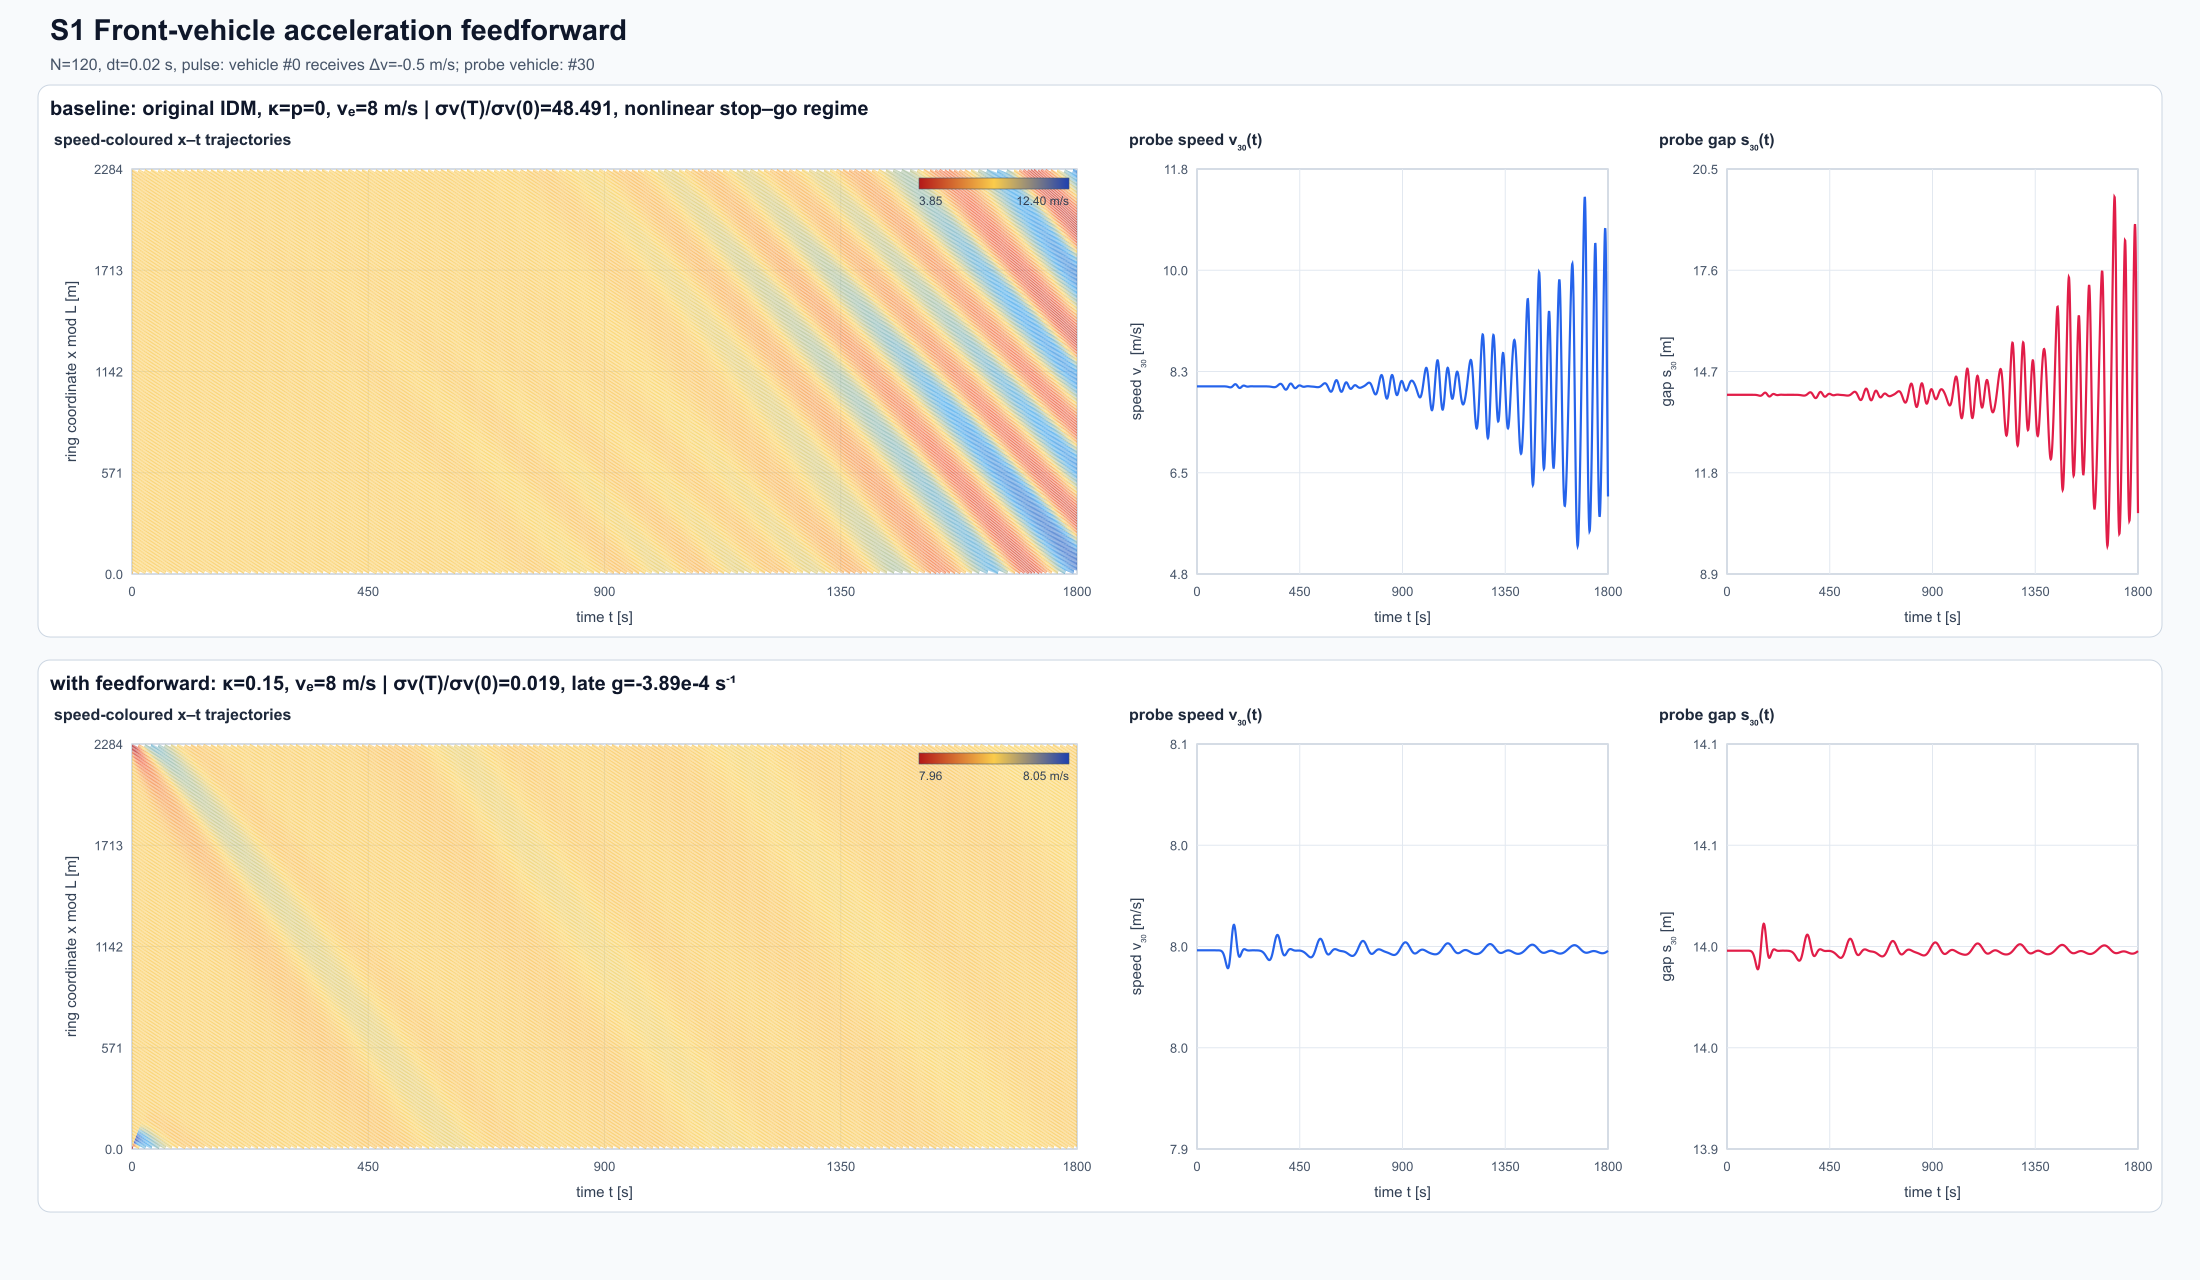
\includegraphics[width=\textwidth]{sim_s1_front_acc.png}
\caption{S1: Trajectory comparison for lead vehicle acceleration feedforward.}
\label{fig:traj-s1}
\figurenote{S1: The Stabilizing Effect of Leading Vehicle Acceleration Feedforward on the Same Instable Traffic Flow. The upper and lower rows of the multiplexed figure ~\ref{fig:traj-s0} and $v_e=8$ share the same operating point (m/s), number of vehicles, initial pulse, color code, and 1,800-second time window; $\kappa=0.15$ is added only to the lower row, thus constituting a controlled single-factor comparison. In the baseline row, the low-speed color band propagates upstream and deepens after each loop, while the probe speed and net spacing increase in sync from peak to peak; after adding feedforward, vehicles receive information about the acceleration of the vehicle ahead in advance, causing the color band to gradually fade as it propagates, and both probe values return to their equilibrium values. This figure illustrates that feedforward does not simply increase the average speed, but rather alters the spatial transfer gain of disturbances, causing the same small pulse to transition from being amplified from vehicle to vehicle to being attenuated from vehicle to vehicle. Combined with $\kappa=0.15>\kappa_c=0.134$, the time-domain recovery aligns with the direction of the analytical threshold, thereby demonstrating that the critical gain has practical control significance.
}
\end{figure}

\section{Tutorial Example M04: No State Reset, Stability Control Enabled Midway}
\sectionstudy{experiment}{Tutorial Example M04: No State Reset, Stability Control Enabled Midway}{milanes2014,ploeg2014,feng2019}




\label{sub:m04-online-control}




Set $N=30$ and $v_e=8$ m/s and increase the initial mode amplitude to $0.2$ m/s so that the oscillation initially develops under the

original IDM conditions. For a duration of $t=300$ s, the acceleration gain of the leading vehicle is increased linearly from 0 to

$\kappa=0.25$ within 60 s; position, velocity, and any fluctuations that have already arisen are fully preserved and not re-initialized.

The analytical root changes from $+0.00408566$ s$^{-1}$ to $-0.0115580$ s$^{-1}$.

The standard deviation of the average velocity from $240$–$300$ s is $0.19319$ m/s, while

that from $780$ to $900$ s dropped to $8.08\times10^{-4}$ m/s, corresponding to a decrease of $99.58\%$.












\begin{figure}[htbp]
\centering
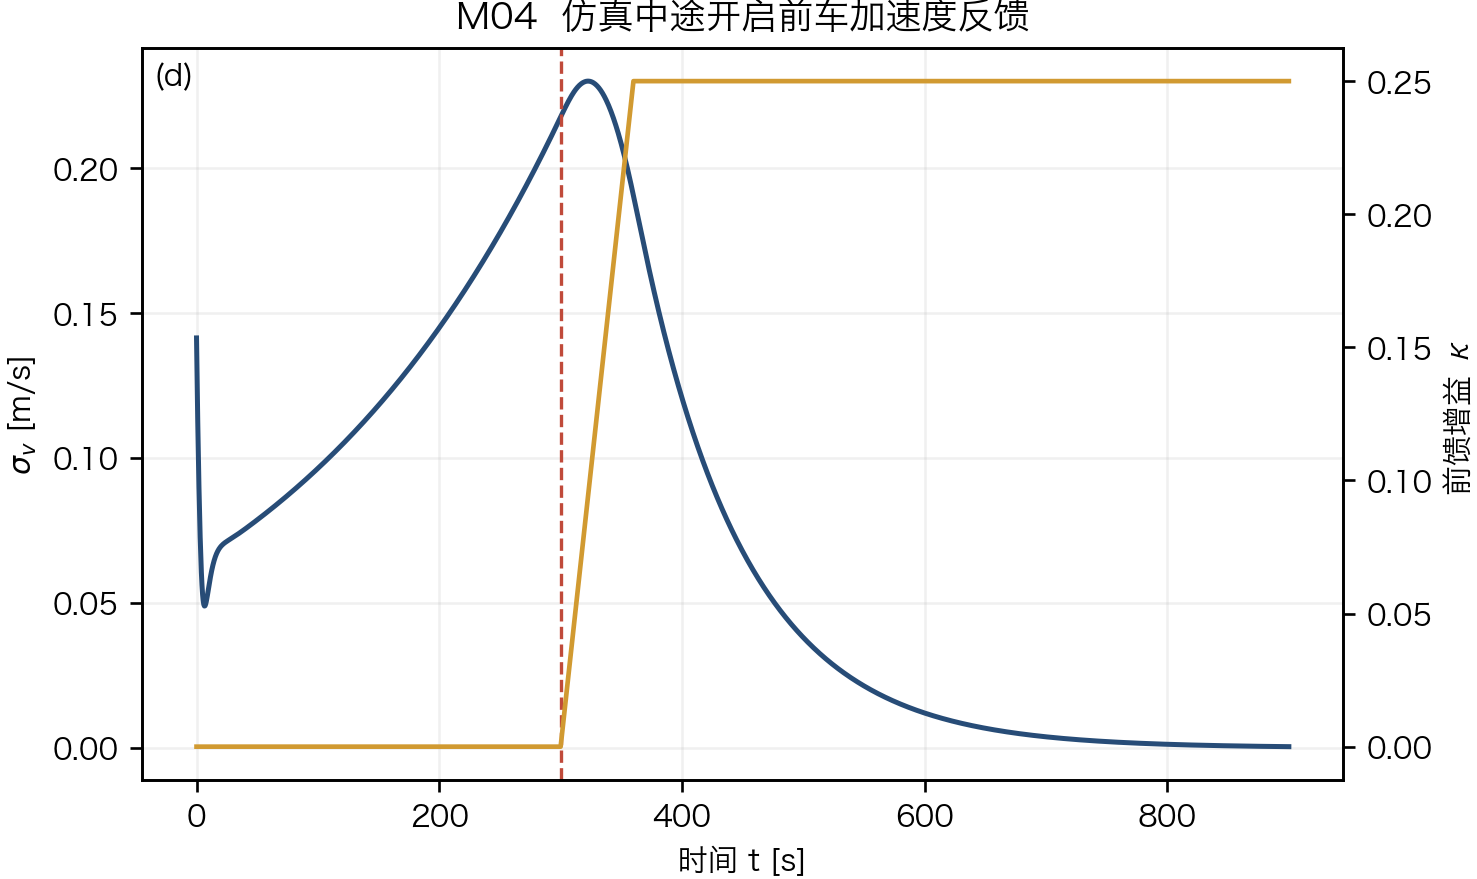
\includegraphics[width=0.88\textwidth]{mini_example_m04.png}
\caption{M04: Activate acceleration feedback of the leading vehicle during travel.}
\label{fig:m04-online-control}
\figurenote{M04: Results of the online switching experiment addressing the question, “Can an established walk-stop wave be eliminated?” At the start of the simulation, the original IDM is maintained, allowing the velocity standard deviation to first increase according to the instability mode; at the red dashed line, neither the position, velocity, nor historical state is reset—only the feedforward gain indicated in yellow is smoothly switched from zero to the stable region. Before the switch, the envelope of the blue $\sigma_v$ curve rises; after the switch, following a brief transition, it turns into a sustained decline, proving that the control alters the system’s current characteristic growth rate rather than relying on reinitialization to produce a smooth curve. If only two independent simulations were compared, the differences might stem from initial conditions; the continuous state transition in this figure eliminates this source of confusion. It also reveals that the control gain has a recovery time: after intervention, the disturbance does not disappear instantly but gradually decays at a new negative growth rate, which is crucial for designing actual control start/stop sequences and duration.}
\end{figure}










A static comparison can only demonstrate that “two fixed parameter points are different”; M04 further illustrates that after a parameter switch,







\textbf{an existing disturbance}




will transition from the growth branch to the decay branch. The gain is varied gradually over 60 s

to prevent the discontinuous switch itself from triggering a high-frequency response.




%==================================================================







\sectionwrapup{Lead-vehicle acceleration feedforward does not alter the local recovery root of a single vehicle, but it reduces the per-vehicle transfer amplitude and expands the linear stability region. M04 further reduces the speed standard deviation by $99.58\%$ without resetting the traffic state, demonstrating the stabilization process under existing disturbances; however, in engineering practice, it is still necessary to jointly verify the peak values at finite frequencies, communication delays, and actuator bandwidth.}

\PART{IV}{Disrupting unidirectional cascading: coupling in the direction of the following vehicle}

\chapter{Further Extension: Simultaneously Considering the Acceleration of the Following Vehicle (Bidirectional Control)}
\label{sec:bilat}
\chapterguide{Why Bidirectional Coupling Causes Scalar Cascades to Fail}{




This chapter constructs complex-coefficient dispersion relations starting from the cyclic shift operator, explains why implicit acceleration coupling must be solved globally, and uses two Bilharz conditions to examine total coupling and finite-wavelength instability, respectively.
}

\section{First, Clarify the Two Meanings of “Rear Car”}
\sectionstudy{theory}{First, Clarify the Two Meanings of “Rear Car”}{swaroop1996,stuedli2017,feng2019}

\begin{itemize}[leftmargin=1.4em,itemsep=3pt]
\item




 If “rear car acceleration” refers to




\textbf{the car’s own}




acceleration $\dot v_n$ appearing on the right-hand side, that is




\textbf{implicit form}




, which has already been




processed in $0.135$: after rearranging terms, it is reduced to the equivalent $f_a$, and the conclusion is that the relative acceleration term has no effect whatsoever on linear stability.







\item




If referring to




\textbf{the acceleration of the vehicle behind}




$n+1$, then it is




\textbf{Bilateral control}




(bilateral / look-back control). This is the subject of this chapter and represents a scenario where the problem is fundamentally altered in terms of structure.







\end{itemize}

\section{Models and Linearization}
\sectionstudy{model}{Modell und Linearisierung}{swaroop1996,stuedli2017,feng2019}












\begin{equation}
\dot v_n = f\left(s_n,\; v_n,\; v_{n-1},\; \dot v_{n-1},\; \dot v_{n+1}\right)
\end{equation}




At the equilibrium point, two new partial derivatives are added:

\begin{equation}
f_a \equiv \frac{\partial f}{\partial \dot v_{n-1}},
\qquad
f_b \equiv \frac{\partial f}{\partial \dot v_{n+1}}
\end{equation}




The equilibrium state remains unchanged (at equilibrium, both accelerations are zero). Linearization:

\begin{equation}
\ddot y_n = f_s\left(y_{n-1}-y_n\right) + f_v\dot y_n + f_{v_l}\dot y_{n-1}
+ f_a\ddot y_{n-1} + f_b\ddot y_{n+1}
\label{eq:bilin}
\end{equation}












\section{Structural change: The transfer function method fails}
\sectionstudy{theory}{Structural change: The transfer function method fails}{swaroop1996,ploeg2014,feng2019}
\label{sub:nofail}

\begin{tcolorbox}[notebox,title=\textbf{Wichtig}]

$y_n$ now depends simultaneously on $y_{n-1}$ and $y_{n+1}$; the chain




\textbf{ist keine unidirektionale Kaskade mehr}






. The $n$ equation cannot be solved without taking $n$ into account—since $Y_{n+1}$, in turn, depends on $Y_n$. The entire team has become a




\textbf{dreitrigonales lineares System}






, such that the concept of the “amplification factor per vehicle” is no longer valid in itself.




One must return to




\textbf{Spatial Fourier analysis / eigenvalue analysis for ring-shaped vehicle platoons}。
\end{tcolorbox}

\textbf{Local stability remains unchanged.} If the two adjacent vehicles in front and behind are both frozen at constant speeds, then $\ddot y_{n\pm1}=0$, the two newly added terms disappear simultaneously, and the characteristic equation remains $\lambda^2-f_v\lambda+f_s=0$.










\section{Why Fourier Modes Can Be Obtained: Cyclic Matrices and DFT}
\sectionstudy{proof}{Why Fourier Modes Can Be Used: Cyclic Matrices and DFT}{swaroop1996,stuedli2017,feng2019}







\label{sub:circulant}




Before deriving the modal solution, let’s clarify that this is not a matter of “guessing a form and trying it out,” but rather a rigorous eigenvalue decomposition.










\subsection{Expressing it in operator form}










Let $\mathbf y=(y_1,\dots,y_N)^T$, and define




\textbf{Cyclic shift operator}




 $S$:

\begin{equation}
\left(S\mathbf y\right)_n = y_{n-1},
\qquad S^N = I \ \ (\text{periodic boundary})
\end{equation}




The “shift” here refers to




\textbf{the shift in vehicle numbers}




—not the actual displacement of the vehicle on the road; $y_n$ represents the positional disturbance of the $n$th vehicle relative to its equilibrium position. $S$ can be understood as an operation to “retrieve data from the preceding vehicle”: it replaces each component of the entire vector with the corresponding component from the preceding vehicle.










\begin{tcolorbox}[experimentbox,title=\textbf{Understanding the shift operator using 4 vehicles as an example}]

If there are 4 vehicles on the racetrack, let

\[
\mathbf y=
\begin{pmatrix}y_1\\y_2\\y_3\\y_4\end{pmatrix},
\qquad
S=
\begin{pmatrix}
0&0&0&1\\
1&0&0&0\\
0&1&0&0\\
0&0&1&0
\end{pmatrix}.
\]




Then




\[
S\mathbf y=
\begin{pmatrix}y_4\\y_1\\y_2\\y_3\end{pmatrix},
\qquad
S^2\mathbf y=
\begin{pmatrix}y_3\\y_4\\y_1\\y_2\end{pmatrix},
\qquad
S^{-1}\mathbf y=
\begin{pmatrix}y_2\\y_3\\y_4\\y_1\end{pmatrix}.
\]




Therefore, $S$ takes the value of the $n-1$-th vehicle (the vehicle ahead), $S^{-1}$ takes the value of the $n+1$-th vehicle (the vehicle behind), and $I$ retains the value of the current vehicle. After four successive cyclic shifts, the vector returns to its original state, such that $S^4=I$ holds; in general, $N$ vehicles have the value $S^N=I$.
\end{tcolorbox}










The linearized equations of the reference model are

\begin{equation}
\ddot{\mathbf y} = \underbrace{f_s\left(S-I\right)}_{A}\mathbf y + \underbrace{\left(f_vI+f_{v_l}S\right)}_{B}\dot{\mathbf y}
\label{eq:shift-baseline}
\end{equation}

$A,B$ are both polynomials of $S$, and therefore both are




\textbf{Cyclic matrix}




. This step relies on two physical assumptions:




\textbf{Uniform fleet}




(all vehicles follow the same rules) and




\textbf{Periodic Boundary}




(subscript modulus $N$).










\subsection{Break down the expression ~\eqref{eq:shift-baseline} term by term back into individual vehicle equations}





The matrix notation does not introduce any new physical assumptions; it simply writes out the equations for all $N$ vehicles at once. Take the $n$th component of expression ~\eqref{eq:shift-baseline}:

\begin{align}
\bigl[(S-I)\mathbf y\bigr]_n
&=(S\mathbf y)_n-(I\mathbf y)_n=y_{n-1}-y_n,\\
\bigl[(f_vI+f_{v_l}S)\dot{\mathbf y}\bigr]_n
&=f_v\dot y_n+f_{v_l}\dot y_{n-1}.
\end{align}

Therefore, when expanded, equation ~\eqref{eq:shift-baseline} is exactly

\begin{equation}
\ddot y_n=f_s(y_{n-1}-y_n)+f_v\dot y_n+f_{v_l}\dot y_{n-1},
\end{equation}

which is the baseline linearized equation for each vehicle. The subscripted brackets are merely used to name the two matrices: $A=f_s(S-I)$ and $B=f_vI+f_{v_l}S$.










\begin{tcolorbox}[notebox,title=\textbf{Why hasn’t Equation ~\eqref{eq:shift-baseline} yet included $f_a$ and $f_b$? }]

Equation ~\eqref{eq:shift-baseline} first uses the reference model to illustrate the structure of “cyclic shifting” and does not omit the bidirectional acceleration term. When written in full vector form, Equation ~\eqref{eq:bilin} should be

\begin{equation}
\left(I-f_aS-f_bS^{-1}\right)\ddot{\mathbf y}
=f_s(S-I)\mathbf y+\left(f_vI+f_{v_l}S\right)\dot{\mathbf y}.
\label{eq:bilin-shift}
\end{equation}

where the $n$th component of $S\ddot{\mathbf y}$ is the acceleration of the leading vehicle $\ddot y_{n-1}$, and the $n$th component of $S^{-1}\ddot{\mathbf y}$ is the acceleration of the rear vehicle, $\ddot y_{n+1}$. A cyclic matrix representing the acceleration acting on the entire vehicle appears on the left-hand side; this is precisely why the system must be solved simultaneously at each simulation step, rather than through sequential calculations for each vehicle.


\end{tcolorbox}

\subsection{Time Domain: Linear with Constant Coefficients}










$A,B$ is a constant matrix (partial derivatives at the equilibrium point); it remains constant when the system is linear, and the solution space is spanned by $e^{\lambda t}$. This is a standard conclusion for ODEs and is independent of the system’s structure.










\subsection{Spatial Part: The cyclic matrix is diagonalized by the DFT basis}










The eigenvectors of $S$ are precisely the discrete Fourier basis $\left(\mathbf w_m\right)_n = e^{ikn}$:

\begin{equation}
\left(S\mathbf w_m\right)_n = e^{ik(n-1)} = e^{-ik}\left(\mathbf w_m\right)_n
\qquad\Longrightarrow\qquad
S\,\mathbf w_m = e^{-ik}\,\mathbf w_m
\end{equation}










\begin{tcolorbox}[notebox]

This incidentally explains the origin of all $e^{-ik}$ mentioned earlier:




\textbf{It is the eigenvalue of the shift operator}




. The $P(k)=1-f_ae^{-ik}-f_be^{ik}$ in multi-train coupling is nothing more than a symbol for the operator $I-f_aS-f_bS^{-1}$.







\end{tcolorbox}










Since $A,B$ are all polynomials of $S$, they share the same eigenvectors as $\mathbf w_m$,




\textbf{and are simultaneously diagonalized by the same set of basis vectors}. $N$ coupled second-order equations are thus decoupled into $N$ independent scalar equations

\begin{equation}
\ddot{\hat y}_m = a(k)\hat y_m + b(k)\dot{\hat y}_m
\end{equation}

Each yields a quadratic characteristic equation. Therefore, “substituting $e^{\lambda t+ikn}$” is




\textbf{an eigenvalue decomposition}




, not a trial solution.










\subsection{Quantization and completeness of $k$}










Periodic boundary conditions $y_{n+N}=y_n$, i.e., $e^{ikN}=1$:

\begin{equation}
k = \frac{2\pi m}{N},\qquad m=0,1,\dots,N-1
\end{equation}

(Since $m$ and $m+N$ represent the same modality, only $N$ is included.)










\textbf{Completeness:}




The state space has $2N$ dimensions ($N$ positions and $+$ $N$ velocities); $N$ modes, $\times$ quadratic equations each with $2$ roots, $=2N$,




\textbf{exactly fills}. Therefore, “checking $\operatorname{Re}\lambda$ for all $m$” is both necessary and sufficient, ensuring no roots are missed.










\subsection{Two Technical Notes}

\begin{itemize}[leftmargin=1.4em,itemsep=4pt]
\item \textbf{$m=0$ must be excluded separately.}




 $\mathbf w_0=(1,\dots,1)^T$, while $A\mathbf w_0=f_s(S-I)\mathbf w_0=0$ ($A$ contains only differences, with a row sum of zero), the characteristic equation degenerates to $P\lambda^2-Q\lambda=0$, and $\lambda=0$ must exist. This zero root corresponds to




\textbf{Global translation}




This trivial symmetry is always neutral.







\item \textbf{Simply scan $k\in(0,\pi]$.}




Since the coefficients of $f_s,f_v,f_{v_l}$ are all real numbers, $\lambda(-k)=\overline{\lambda(k)}$ and $\operatorname{Re}\lambda$ are even functions with respect to $k$, and $k$ and $2\pi-k$ yield the same growth rate.







\end{itemize}

\begin{tcolorbox}[notebox,title=\textbf{When does this assumption fail?}]
\begin{itemize}[leftmargin=1.2em,itemsep=2pt]
\item \textbf{The fleet is heterogeneous.}($F_n\ne F_{n-1}$) The $\Rightarrow$ matrix is no longer cyclic, and the DFT basis is no longer diagonalized—see Chapter ~\ref{sec:het}~;







\item \textbf{Open chain rather than a loop}




$\Rightarrow$ has no periodic boundary, $k$ is not quantized; the correct object is the transfer function (Chapter ~\ref{sec:appx}~ proves that the two are equivalent when proving $N\to\infty$);







\item \textbf{With lane changes or heterogeneous perturbations}




 $\Rightarrow$ Translation invariance is violated.







\end{itemize}
\end{tcolorbox}

\section{Characteristic equation of a ring-shaped convoy}
\sectionstudy{model}{Characteristic equation of a ring-shaped convoy}{swaroop1996,stuedli2017,feng2019}










Let $N$ vehicles be on the ring track; take the modal

\begin{equation}
y_n(t) = \hat y\,e^{\lambda t + ikn},
\qquad
k = \frac{2\pi m}{N},\quad m=0,1,\dots,N-1
\end{equation}




Substitute into the equation ~\eqref{eq:bilin} (note $y_{n\pm1}=y_n e^{\pm ik}$) and simplify:







\begin{tcolorbox}[keybox]
\begin{equation}
P(k)\,\lambda^2 - Q(k)\,\lambda - R(k) = 0
\end{equation}
\begin{equation}
P(k) = 1 - f_a e^{-ik} - f_b e^{ik},
\qquad
Q(k) = f_v + f_{v_l}e^{-ik},
\qquad
R(k) = f_s\left(e^{-ik}-1\right)
\end{equation}
\end{tcolorbox}










Stability requirement: For each $k\ne0$, both roots lie in the left half-plane. $k=0$ corresponds to a global translation and is always a neutral mode.










\section{Criteria for complex-coefficient quadratic equations (Bilharz criterion)}
\sectionstudy{proof}{Stability Criteria for Quadratic Equations with Complex Coefficients (Bilharz Criteria)}{swaroop1996,stuedli2017,feng2019}










Since $P,Q,R$ consists entirely of complex numbers, the Routh–Hurwitz criterion for real coefficients cannot be applied directly. Convert to leading-1 form

\begin{equation}
\lambda^2 + c_1\lambda + c_0 = 0,
\qquad
c_1 = -\frac{Q}{P} = p_1 + iq_1,
\qquad
c_0 = -\frac{R}{P} = p_2 + iq_2
\end{equation}










\begin{tcolorbox}[keybox,title=\textbf{Stability Criteria for Complex-Coefficient Quadratic Polynomials}]

Both roots satisfy $\operatorname{Re}\lambda<0$ if and only if

\begin{equation}
p_1 > 0
\qquad\text{and}\qquad
\Delta_2 \equiv p_1\left(p_1p_2 + q_1q_2\right) - q_2^2 > 0
\end{equation}







\end{tcolorbox}










The complete proof of the criterion is given in Appendix ~\ref{sec:theorem-reference}: First, using Viète’s formulas, express $p_j,q_j$ as a combination of the real and imaginary parts of the two roots, then prove that

\begin{equation}
\Delta_2 = \alpha_1\alpha_2\left[\left(\alpha_1+\alpha_2\right)^2 + \left(\beta_1-\beta_2\right)^2\right].
\end{equation}

Therefore, $p_1>0$ and $\Delta_2>0$ precisely rule out any single one from entering the closed right-half-plane. The real-coefficient Routh–Hurwitz criterion cannot be directly applied here, because $c_1,c_0$ is generally not a real number.










\section{Simplification: Conditions for two real polynomials}
\sectionstudy{theory}{Simplification: Conditions for two real polynomials}{swaroop1996,stuedli2017,feng2019}


\label{sub:twocond}




Let

\begin{equation}
u = \cos k \in [-1,\,1),
\qquad
\sigma = f_a+f_b \ \ (\text{total coupling strength}),
\qquad
d = f_a-f_b \ \ (\text{asymmetry})
\end{equation}




First, let’s break down “algebraic simplification” into a traceable path; all multiplications and coefficients are listed in Appendix ~\ref{sec:bilharz-algebra}. Let

\begin{equation}
s_k=\sin k,
\qquad
D(u)=|P(k)|^2=(1-\sigma u)^2+d^2(1-u^2).
\label{eq:D-bilateral}
\end{equation}

In the regular case of $P(k)\ne0$ (i.e., $D>0$), after multiplying by the conjugate $\overline P$, the four real coefficients can be written as

\begin{align}
p_1&=\frac{\Pi(u)}{D(u)},
&q_1&=\frac{s_k\,\Xi(u)}{D(u)},\\
p_2&=\frac{f_s(1-u)\,\Gamma(u)}{D(u)},
&q_2&=\frac{f_ss_k\,\Omega(u)}{D(u)},
\label{eq:pq-bilateral}
\end{align}

where

\begin{align}
\Pi(u)&=-\left(f_v+f_{v_l}u\right)+\sigma f_vu+f_{v_l}\left(d+2f_bu^2\right),\\
\Xi(u)&=d\left(f_v+f_{v_l}u\right)+f_{v_l}(1-\sigma u),\\
\Gamma(u)&=1+d-2f_bu,
&\Omega(u)&=1-d-2f_bu.
\label{eq:aux-bilateral}
\end{align}




The first Bilharz condition immediately becomes

\begin{equation}
p_1>0
\iff
\frac{\Pi(u)}{D(u)}>0
\iff
\Pi(u)>0,
\end{equation}

because $D(u)>0$. The second condition appears more complex, but upon substituting ~\eqref{eq:pq-bilateral}, all higher-order terms factor exactly into

\begin{equation}
\Delta_2
=p_1(p_1p_2+q_1q_2)-q_2^2
=\frac{f_s(1-u)}{D(u)^2}\,\widetilde W(u).
\label{eq:Delta-factor}
\end{equation}

For the non-trivial modal $k\ne0$, we have $f_s>0$, $1-u>0$, and $D^2>0$; therefore, the sign of $\Delta_2$ is determined solely by $\widetilde W$. Thus, the two conditions can be expressed as:










\begin{tcolorbox}[keybox,title=\textbf{Condition I}]
\begin{equation}
\Pi(u) \equiv -\left(f_v + f_{v_l}u\right) + \sigma f_v u + f_{v_l}\left(d + 2f_b u^2\right) \;>\; 0
\label{eq:Pi-bilateral}
\end{equation}
\end{tcolorbox}

\begin{tcolorbox}[keybox,title=\textbf{Condition II}]
\begin{equation}
\widetilde W(u) = w_3u^3 + w_2u^2 + w_1u + w_0 \;>\; 0
\label{eq:Wpoly-bilateral}
\end{equation}
\begin{align}
w_3 &= -4f_b^2 f_s \\
w_2 &= 2f_b\left[2f_s\left(1-f_a\right) + f_{v_l}\left(f_{v_l}-f_v\right)\right] \\
w_1 &= -f_s\left(1-\sigma\right)^2 + 4f_b^2f_s - \sigma f_v^2 + \left(1+\sigma\right)f_vf_{v_l} - f_{v_l}^2 \\
w_0 &= -f_s\left(1-d\right)^2 + f_v^2 - f_vf_{v_l} + d\,f_{v_l}\left(f_{v_l}-f_v\right)
\label{eq:Wcoeff-bilateral}
\end{align}
\end{tcolorbox}










The two endpoint values are particularly concise:

\begin{align}
\widetilde W(1) &= \left(1-\sigma\right)\left[f_v^2 - f_{v_l}^2 - 2f_s\left(1-\sigma\right)\right]
\label{eq:W1}\\
\widetilde W(-1) &= \left(1+\sigma\right)\left(f_v-f_{v_l}\right)^2
\end{align}

\begin{equation}
\Pi(1) = \left(\sigma-1\right)\left(f_v+f_{v_l}\right)
\end{equation}










\section{Three closed-form conclusions}
\sectionstudy{theory}{Three Closed-Form Conclusions}{swaroop1996,stuedli2017,feng2019}

\begin{tcolorbox}[keybox,title=\textbf{(A) Upper Bound on the Total Coupling Strength}]

From $\Pi(1)>0$ and $f_v+f_{v_l}<0$:

\begin{equation}
\sigma = f_a + f_b \;<\; 1
\end{equation}

and then from $\widetilde W(-1)>0$, we obtain $\sigma>-1$. Therefore,




\textbf{Necessary condition: $\left|f_a+f_b\right|<1$}。
\end{tcolorbox}

\begin{tcolorbox}[keybox,title=\textbf{(B) Long-wave condition: Depends only on $f_a+f_b$}]

From equations \eqref{eq:W1} and $\sigma<1$:

\begin{equation}
\frac{1}{2}\left(f_v^2 - f_{v_l}^2\right) \;\ge\; \left(1-f_a-f_b\right)f_s
\end{equation}







\textbf{The forward and backward acceleration feedbacks are completely equivalent on the long-wave scale; only the sum $\sigma$ is effective.}




(This can be independently verified via long-wave expansion: $c_1=V'(s_e)$ remains unchanged, in the expression for $c_2$, $f_a$ is precisely replaced by $\sigma$, and the asymmetry $d$ does not appear until $O(\varepsilon^3)$.)







\end{tcolorbox}

\begin{tcolorbox}[keybox,title=\textbf{(C) Finite-wavelength conditions: Asymmetry comes into play here}]

$\widetilde W$ is the




\textbf{third-order}




polynomial, with the leading coefficient being $w_3=-4f_b^2f_s\le0$. When $f_b\ne0$, the curve may cross zero inside the interval; in this case, the endpoint test




\textbf{is no longer sufficient}




; $u\in[-1,1)$ must be scanned.







\end{tcolorbox}

\section{Three special cases}
\sectionstudy{theory}{Three Special Cases}{swaroop1996,stuedli2017,feng2019}
\label{sub:special}

\textbf{(1) $f_b=0$ (purely forward-looking; see Chapter ~\ref{sec:lead}~).
}




 In this case, $w_3=w_2=0$ and $\widetilde W$ degenerate into




\textbf{linear}




functions, and the minimum must be attained at the endpoints, subject to the condition

\begin{equation}
\left|f_a\right| \le 1
\qquad\text{and}\qquad
\frac{1}{2}\left(f_v^2-f_{v_l}^2\right) \ge \left(1-f_a\right)f_s
\end{equation}

—and




the result obtained using the transfer function for \ref{sub:leadcond}




\textbf{are completely consistent}




. This simultaneously cross-validates the two sets of methods.










\textbf{(2) $f_b=f_a$ (symmetric bidirectional).} At this point, $P = 1-2f_a\cos k$ is




\textbf{a real number}




, and $d=0$ and $\widetilde W$ can be factored as follows:

\begin{equation}
\widetilde W(u) = \left(1-2f_au\right)B(u),
\qquad
B(u) = 2f_af_su^2 + \left[2f_af_s - f_s + f_vf_{v_l} - f_{v_l}^2\right]u + \left[f_v^2-f_vf_{v_l}-f_s\right]
\end{equation}

where $1-2f_au>0$ holds for all $u$, which is consistent with Conclusion (A). All that remains is $B(u)>0$.










\textbf{(3) $f_a=0$ (pure back-looking).}




$\widetilde W$ is a complete cubic expression, $w_3<0$. Numerically, we observe that the system remains stable when the gain is small, but




\textbf{becomes unstable once the gain increases to a certain intermediate value}




—the acceleration coupling in the pure lookback configuration leads to self-excitation in the short-wavelength range.










\section{Numerical example}
\sectionstudy{experiment}{Numerical example}{swaroop1996,stuedli2017,feng2019}







\label{sub:multinum}




Using the IDM parameters from Chapter ~\ref{sec:num}~, calculations were performed at $v_e=8$ m/s (the reference model is linearly unstable at this value):

\[
f_s = 0.1421,\qquad f_v = -0.6803,\qquad f_{v_l} = 0.4650
\]

The long-wave threshold is

\[
\sigma \;\ge\; 1 - \frac{f_v^2-f_{v_l}^2}{2f_s} = 0.133
\]





\begin{figure}[htbp]
\centering
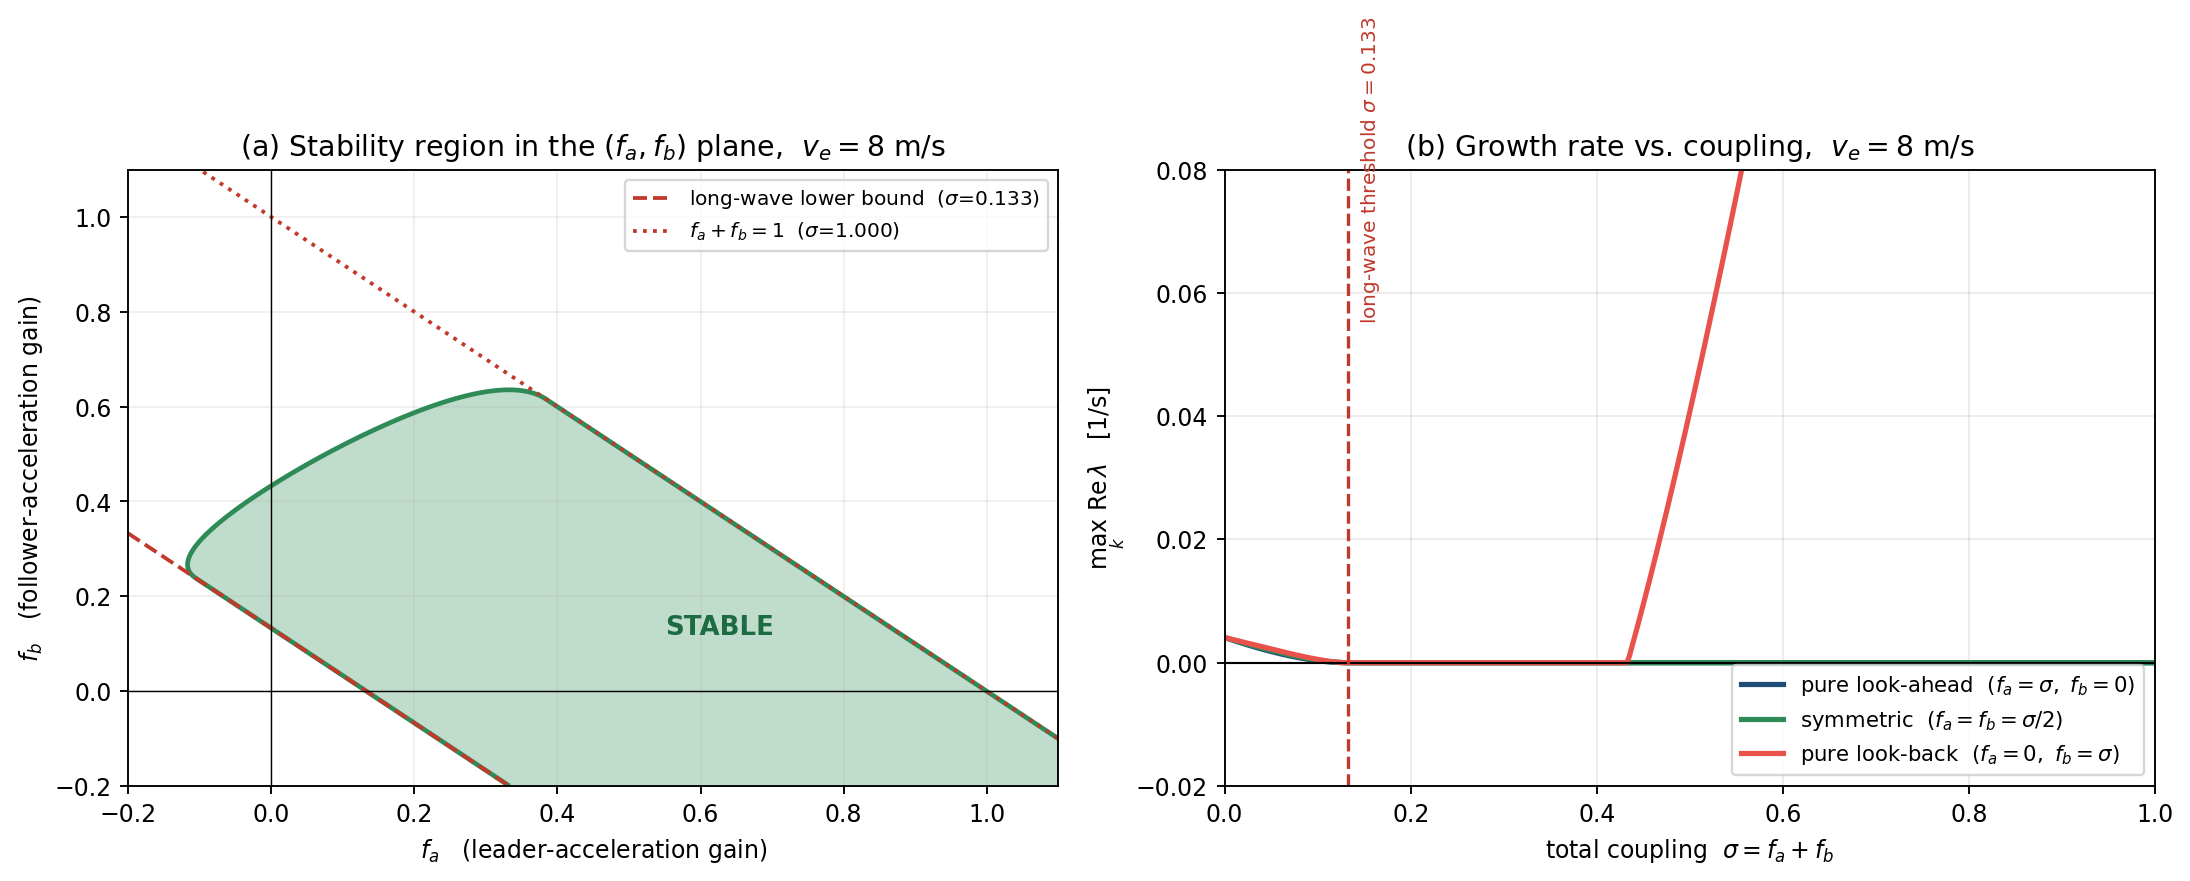
\includegraphics[width=\textwidth]{fig2.png}
\caption{Stability Region and Growth Rate of Bidirectional Acceleration Coupling.}
\label{fig:bilateral-domain}
\figurenote{The complete stability region of bidirectional acceleration coupling and the principle that “equal total quantities do not imply identical full spectra.” The left figure shows a point-by-point scan of all discrete wavenumbers in the $(f_a,f_b)$ plane. The straight lower boundary of the stability region is determined by the long-wave threshold of $f_a+f_b$, while the curved upper boundary arises from a finite $k$ mode first crossing the imaginary axis; Therefore, examining only $k\to0$ would incorrectly classify points outside the curved boundary as stable. The figure on the right changes the horizontal axis to the total coupling $\sigma=f_a+f_b$ and compares three allocation schemes: pure forward-looking, mixed, and pure backward-looking; the three curves simultaneously cross the zero line at approximately $0.133$, demonstrating that zero-order total control determines the starting point of long waves. As $\sigma$ continues to increase, the forward-looking scheme continues to improve, while the pure backward-looking scheme re-exhibits a positive growth rate at approximately $0.43$, revealing that the first-order moment in the backward direction erodes the finite wavelength margin. This figure demonstrates that the control design must be conducted in two steps: First, use total control to cross the long-wave threshold, then use a full-wavenumber scan to eliminate secondary instability caused by allocation.}
\end{figure}

\begin{tcolorbox}[notebox,title=\textbf{Engineering Conclusions}]
\begin{itemize}[leftmargin=1.2em,itemsep=3pt]
\item




To eliminate stop-and-go waves, the key is




\textbf{the total amount of acceleration feedback}




$f_a+f_b$ must reach the threshold; both forward-looking and backward-looking feedback can contribute to this.







\item




However,




\textbf{backward-looking feedback alone cannot bear too much of the burden}: If $f_b$ is too large, it will introduce a new instability branch in the short-wavelength range. The stability region is significantly narrower in the $f_b$ direction than in the $f_a$ direction.







\item




 The total coupling must satisfy $f_a+f_b<1$, which is a hard upper bound.







\item




 Overall,




\textbf{a configuration where forward-looking is the primary focus and backward-looking is secondary}




(the region within the stability domain where $f_a$ is high and $f_b$ is moderate) offers the greatest margin. This aligns with the design approach in CACC practice, which prioritizes information from the vehicle ahead.







\end{itemize}
\end{tcolorbox}

\section{Numerical Validation E3: Bidirectional Implicit Coupling}
\sectionstudy{experiment}{Numerical Validation E3: Bidirectional Implicit Coupling}{swaroop1996,stuedli2017,feng2019}










Using $N=120$ and $v_e=8$ (m/s), compare the baseline model with $(f_a,f_b)=(0.30,0.10)$, which employs a “forward-looking-first, backward-looking-second” approach. For each RK4 substep, solve the cyclic linear system $(I-f_aS-f_bS^{-1})\bm a=\bm a_{\rm IDM}$, with the residual threshold set to $10^{-9}$.










\begin{center}
\small
\captionof{table}{Dominant modes and growth rates for E3 bidirectional implicit coupling.}
\label{tab:e3-bilateral}
\begin{tabular}{p{3.4cm}p{3.2cm}p{3.4cm}p{3.2cm}}
\toprule
\textbf{Scenario} & \textbf{$m^*$} & \textbf{$\max\operatorname{Re}\lambda$ [s$^{-1}$]} & \textbf{Results} \\
\midrule







S0 Reference IDM& 4 & $+0.00408566$ & Perturbation Growth



\\
S2：$f_a=0.30,f_b=0.10$ & 1 & $-0.00148012$ &




 Perturbation Decay



\\
\bottomrule
\end{tabular}
\end{center}
\tabletext{tab:e3-bilateral}{




Dominant modes and the rightmost root for the reference IDM and bidirectional coupling conditions. After the total feedback is 0.40, the growth rate changes from positive to negative, verifying the consistency between the iterative implicit solution and the Fourier eigenvalues.
}










The parameter scan also provides a full-speed-range window for pure positive feedback of approximately $0.134\le f_b\le0.43$: the lower boundary is determined by the total long-wave amplitude, and the upper boundary is determined by the finite wavelength. Therefore, the test report must provide both $m^*$ and the rightmost root; it is not sufficient to merely verify whether $f_a+f_b$ exceeds the long-wave threshold.










\begin{tcolorbox}[resultbox,title=\textbf{Verification Conclusions}]

After incorporating the bidirectional acceleration feedback of the total quantity $f_a+f_b=0.40$, the rightmost root shifts from $+4.09\times10^{-3}$ to $-1.48\times10^{-3}$ s$^{-1}$. The iterative implicit solution and the Fourier eigenvalues yield the same stability sign; If explicitly replaced with “previous acceleration,” additional phase errors are introduced near the critical point, which is not considered quantitative evidence.







\end{tcolorbox}

\section{Specific trajectory results: Bidirectional acceleration coupling}
\sectionstudy{experiment}{Specific trajectory results: Bidirectional acceleration coupling}{ngsim2016,thiemann2008,krajewski2018}





Figure ~ \ref{fig:traj-s2}: $(f_a,f_b)=(0.30,0.10)$ is added at the same $v_e=8$ m/s instability point. The ratio of the initial to final perturbation for the entire vehicle decreases from the baseline value of $48.49$ to $0.00106$, with a final segment slope of $-1.48\times10^{-3}$ s$^{-1}$, consistent with the rightmost characteristic root in this chapter. The speed of the 30th car varies only within the range of $7.9981$–$8.0017$ m/s, and the spacing varies only within the range of $14.0326$–$14.0381$ m.










\begin{figure}[htbp]
\centering
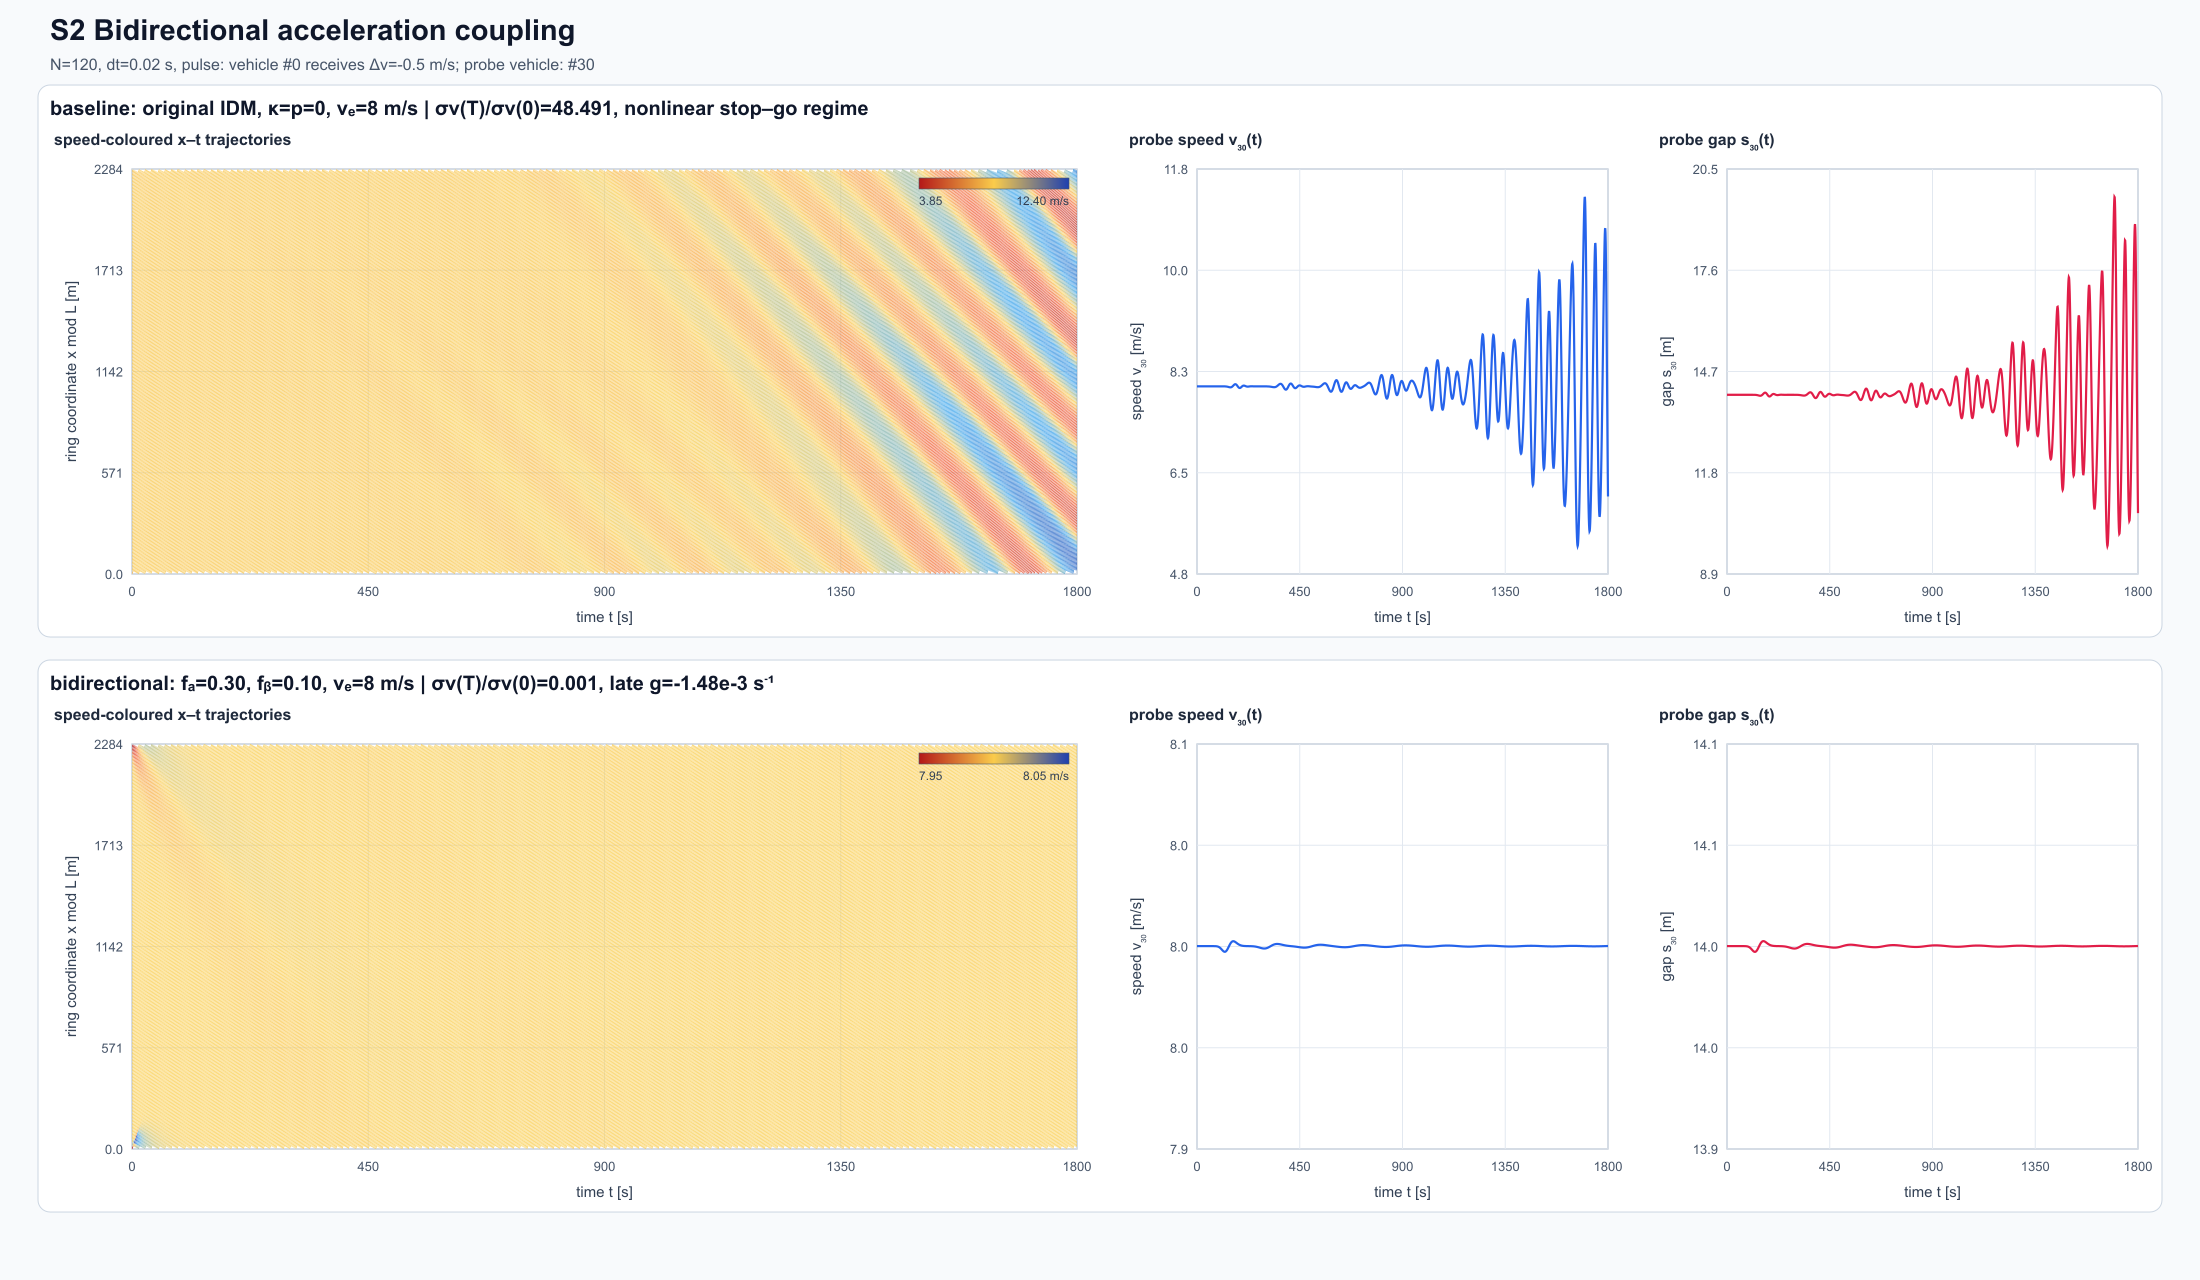
\includegraphics[width=\textwidth]{sim_s2_bilateral_acc.png}
\caption{S2: Trajectory comparison with bidirectional acceleration coupling.}
\label{fig:traj-s2}
\figurenote{S2: Time-domain verification of bidirectional implicit acceleration coupling. The upstream simulation remains the original IDM instability benchmark, while the downstream simulation only incorporates $(f_a,f_b)=(0.30,0.10)$; the number of vehicles, operating points, disturbances, and color codes remain unchanged. Since each vehicle’s acceleration depends simultaneously on the accelerations of its front and rear neighbors, the downstream simulation solves a cyclic linear system at each RK4 substep rather than explicitly substituting the acceleration from the previous step; this prevents numerical lag from skewing the stability conclusions. The results show that the diagonal color bands in the upstream direction intensify with each lap, while the color bands in the downstream direction dissipate as they propagate; the peak values of the specified vehicle’s velocity and inter-vehicle distance also decrease in tandem. This figure not only demonstrates that this parameter point lies within the stability region of Figure ~\ref{fig:bilateral-domain} but also illustrates that the negative growth rate predicted by the complex coefficient spectrum can be achieved in a fully nonlinear, implicitly coupled simulation.}
\end{figure}

%==================================================================
\sectionwrapup{After incorporating the acceleration of the following vehicle, the vehicle accelerations become cyclically coupled at the same instant, rendering the scalar transfer function per vehicle invalid; each product term requires solving a cyclic linear system. Stability is determined jointly by the characteristic equation of the complex-coefficient loop and two real conditions; it cannot be assessed solely based on the long-wave threshold.}

\chapter{Further generalization: Acceleration feedback involving multiple leading and trailing vehicles}
\label{sec:multi}
\chapterguide{Whether the benefit of multi-vehicle information depends on the total amount or spatial distribution}{




This chapter compresses arbitrary forward and backward acceleration kernels into the complex function $P(k)$, using zero-order and first-order moments to separate the long-wave budget from the finite-wavelength cost. The goal is to progress from “seeing more” to a computable gain allocation principle.
}










This chapter does not consider latency for the time being.










\section{Model: Exponentially Decaying Weights}
\sectionstudy{model}{Model: Exponentially Decaying Weights}{lenz1999,feng2019}










The vehicle simultaneously receives acceleration data from $j$ vehicles ahead and $j$ vehicles behind, with weights exponentially decaying according to vehicle order:

\begin{equation}
\dot v_n = F\left(s_n,v_n,\dv_n\right)
+ \sum_{j\ge1} f_a\,\alpha^{\,j-1}\,\dot v_{n-j}
+ \sum_{j\ge1} f_b\,\beta^{\,j-1}\,\dot v_{n+j},
\qquad 0\le\alpha,\beta<1
\end{equation}




$f_a,f_b$ is




\textbf{Nearest Neighbor}




the feedback coefficient, and $\alpha,\beta$ is the attenuation factor. The total feedback amount is

\begin{equation}
\sum_{j\ge1}f_a\alpha^{j-1} = \frac{f_a}{1-\alpha},
\qquad
\sum_{j\ge1}f_b\beta^{j-1} = \frac{f_b}{1-\beta}
\end{equation}










\section{Spatial Fourier: Coupling Function\texorpdfstring{$P(k)$}{P(k)}}
\sectionstudy{theory}{Spatial Fourier: Coupling Function\texorpdfstring{$P(k)$}{P(k)}}{lenz1999,feng2019}





Substituting $y_{n\mp j}=y_n e^{\mp ijk}$, both geometric series can be summed:

\begin{equation}
\sum_{j\ge1}f_a\alpha^{j-1}e^{-ijk} = \frac{f_a e^{-ik}}{1-\alpha e^{-ik}},
\qquad
\sum_{j\ge1}f_b\beta^{j-1}e^{ijk} = \frac{f_b e^{ik}}{1-\beta e^{ik}}
\end{equation}




Consequently, the form of the characteristic equation is exactly the same as in Chapter ~\ref{sec:bilat}~:

\begin{equation}
P(k)\,\lambda^2 - Q(k)\,\lambda - R(k) = 0,
\qquad
P(k) = 1 - \frac{f_a e^{-ik}}{1-\alpha e^{-ik}} - \frac{f_b e^{ik}}{1-\beta e^{ik}}
\end{equation}

Meanwhile, the structures of $Q=f_v+f_{v_l}e^{-ik}$ and $R=f_s(e^{-ik}-1)$ remain unchanged.










\begin{tcolorbox}[notebox]
\textbf{All the complexity of the acceleration coupling is condensed into a single complex function, $P(k)$.}




 This suggests that by reworking the derivations in Chapter ~\ref{sec:bilat}~ for




\textbf{any}




$P$, we can cover all cases at once.







\end{tcolorbox}

\section{Unified Framework: Two Conditions for Arbitrary Acceleration Kernels}
\sectionstudy{theory}{Unified Framework: Two Conditions for Arbitrary Acceleration Kernels}{lenz1999,feng2019}










Let the spatial transformation of the acceleration coupling kernel be

\begin{equation}
P(k) = 1 - \sum_{j\ge1}a_j e^{-ijk} - \sum_{j\ge1}b_j e^{ijk} \;\equiv\; P_r(k) + i\,P_i(k)
\end{equation}




By reformulating the Bilharz criteria (denoted as $u=\cos k$ and $q=\sin k$) for the general complex case $P$, we obtain










\begin{tcolorbox}[keybox,title=\textbf{Condition I}]
\begin{equation}
\Pi(k) = P_i\,f_{v_l}\,q - P_r\left(f_v + f_{v_l}u\right) \;>\; 0
\end{equation}
\end{tcolorbox}

\begin{tcolorbox}[keybox,title=\textbf{Condition II}]
\begin{equation}
\begin{aligned}
\widetilde W(k)={}&P_r\Big[f_v^2-f_{v_l}^2u+f_vf_{v_l}(u-1)-f_s(1+u)P_r\Big]\\
&+P_i q\Big[2f_sP_r-f_{v_l}(f_v-f_{v_l})\Big]
-f_s(1-u)P_i^2>0
\end{aligned}
\end{equation}
\end{tcolorbox}





Two endpoints (here, $q=0$; since all kernels considered in this book satisfy $P_i\propto q$, $P_i=0$ applies):

\begin{align}
\Pi\big|_{k=0} &= -P(0)\left(f_v+f_{v_l}\right) \\
\widetilde W\big|_{k=0} &= P(0)\Big[f_v^2 - f_{v_l}^2 - 2f_s\,P(0)\Big]
\label{eq:Wend}\\
\widetilde W\big|_{k=\pi} &= P(\pi)\left(f_v-f_{v_l}\right)^2
\end{align}










\begin{tcolorbox}[notebox,title=\textbf{Backward Compatibility Check}]
\begin{itemize}[leftmargin=1.2em,itemsep=2pt]
\item




$P\equiv1$ (without acceleration feedback): $\widetilde W = \left(f_v^2-f_vf_{v_l}-f_s\right)+u\left(f_vf_{v_l}-f_{v_l}^2-f_s\right)$, i.e., the benchmark results in Chapter ~\ref{sec:string}~.







\item




$P=1-f_ae^{-ik}$: See Chapter ~\ref{sec:lead}~.







\item




$P=1-f_ae^{-ik}-f_be^{ik}$: That is, Chapter ~\ref{sec:bilat}~, $P(0)=1-\sigma$; the two endpoint formulas match those there word for word.







\end{itemize}
\end{tcolorbox}

\section{Exponential decaying kernel\texorpdfstring{$P_r$ and $P_i$}{Real Part and Imaginary Part}}
\sectionstudy{theory}{Exponential Decay Kernel \texorpdfstring{ $P_r$ and $P_i$ }{ Real Part and Imaginary Part}}{lenz1999,feng2019}





The key is this identity (where the numerator and denominator are conjugate):

\begin{equation}
\frac{e^{-ik}}{1-\alpha e^{-ik}} = \frac{\left(\cos k-\alpha\right) - i\sin k}{1-2\alpha\cos k+\alpha^2}
\end{equation}




Let $D_\alpha = 1-2\alpha u+\alpha^2>0$ and $D_\beta = 1-2\beta u+\beta^2>0$ (which is always positive when $|\alpha|,|\beta|<1$) be defined, then










\begin{tcolorbox}[keybox]
\begin{equation}
P_r = 1 - \frac{f_a\left(u-\alpha\right)}{D_\alpha} - \frac{f_b\left(u-\beta\right)}{D_\beta},
\qquad
P_i = s\left(\frac{f_a}{D_\alpha} - \frac{f_b}{D_\beta}\right)
\end{equation}
\end{tcolorbox}










Substituting $u=1$ ($D_\alpha=(1-\alpha)^2$) and $u=-1$ ($D_\alpha=(1+\alpha)^2$):

\begin{equation}
P(0) = 1 - \underbrace{\left(\frac{f_a}{1-\alpha} + \frac{f_b}{1-\beta}\right)}_{\textstyle \sigma_{\rm eff}},
\qquad
P(\pi) = 1 + \frac{f_a}{1+\alpha} + \frac{f_b}{1+\beta}
\end{equation}










\section{Closed-form conclusion}
\sectionstudy{theory}{Closed-form conclusion}{lenz1999,feng2019}

\begin{tcolorbox}[keybox,title=\textbf{(A) Upper bound on the total feedback}]

From $\Pi(0)>0$ and $f_v+f_{v_l}<0$:

\begin{equation}
\sigma_{\rm eff} = \frac{f_a}{1-\alpha} + \frac{f_b}{1-\beta} \;<\; 1
\end{equation}







\end{tcolorbox}

\begin{tcolorbox}[keybox,title=\textbf{(B) Short-wave condition}]

Given $\widetilde W(\pi)>0$:

\begin{equation}
1 + \frac{f_a}{1+\alpha} + \frac{f_b}{1+\beta} \;>\; 0
\end{equation}

This condition is automatically satisfied when $f_a,f_b\ge0$ holds.







\end{tcolorbox}

\begin{tcolorbox}[keybox,title=\textbf{(C) Long-wave condition: Depends only on $\sigma_{\rm eff}$ }]

Satisfied automatically by the expression ~\eqref{eq:Wend} and $P(0)>0$:

\begin{equation}
\frac{1}{2}\left(f_v^2-f_{v_l}^2\right) \;\ge\; \left(1-\sigma_{\rm eff}\right)f_s
\end{equation}


\textbf{Regardless of whether the feedback is concentrated on the nearest neighbors or distributed across many vehicles, the long-wave threshold considers only the total amount $\sigma_{\rm eff}$.
}




This is a natural generalization of the conclusion (B) in Chapter ~\ref{sec:bilat}~.







\end{tcolorbox}

\begin{tcolorbox}[keybox,title=\textbf{(D) Finite Wavelength Condition}]

It is also required that $\Pi(k)>0$ and $\widetilde W(k)>0$ hold within $k\in(0,\pi]$. $\alpha,\beta$ appears in the denominator of $D_\alpha,D_\beta$, causing $\widetilde W$ to no longer be a polynomial; generally, a numerical scan is required.







\end{tcolorbox}

\section{Numerical Example}
\sectionstudy{experiment}{Numerical Example}{lenz1999,feng2019}










Still using the IDM parameters from Chapter ~\ref{sec:num}~, the requirement is




\textbf{Full speed range}




Linear stability. The most stringent long-wave threshold across the full speed range is

\begin{equation}
\sigma_c = \max_{v_e}\left[1-\frac{f_v^2-f_{v_l}^2}{2f_s}\right] = 0.1336
\end{equation}










\begin{figure}[htbp]
\centering
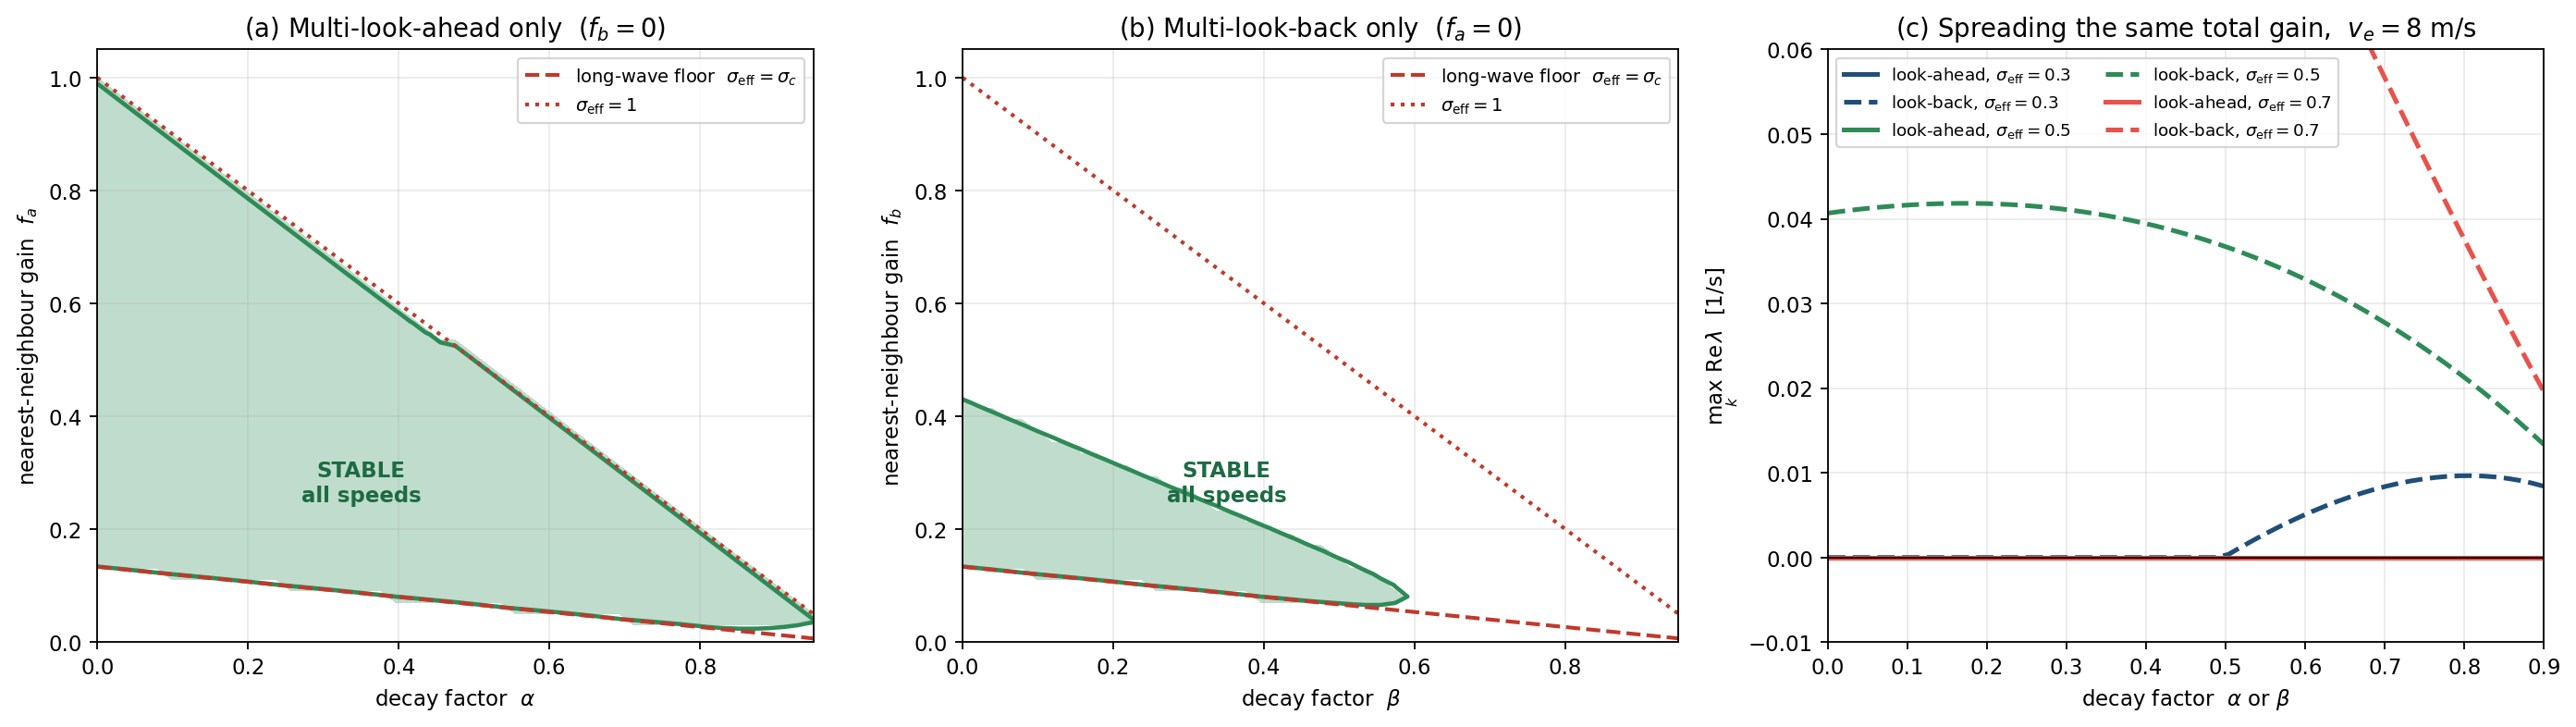
\includegraphics[width=\textwidth]{fig5.png}
\caption{Stability region with feedback from multiple leading and trailing vehicles.}
\label{fig:multi-domain}
\figurenote{Comparison of the stability regions for multi-forward and multi-rear vehicle index kernels. In the left figure, only the forward-looking kernel is retained; the stability region varies with the decay factor and nearest-neighbor gain, and is bounded by two closed boundaries: the lower limit of total feedback and the upper limit at high frequencies. This indicates that forward information can be distributed among more vehicles while keeping the total amount constant. The middle figure retains only the backward-looking kernel; the stable region shrinks significantly, and the stable solution disappears entirely when the decay is too slow or the weight of distant rear vehicles accumulates excessively, indicating that “seeing farther” in the backward direction may amplify erroneous phases. The right figure fixes the zero-order total and only alters the spatial range of the kernel: all curves share the same starting point at $k\to0$ but clearly diverge at finite wavenumbers, directly demonstrating that first-order moments—rather than the number of vehicles itself—control the margin in the short-to-medium-wavelength range. This figure proves that the evaluation of multi-vehicle communication cannot simply state “how many vehicles were received”; it must also report the direction, individual weights, and kernel moments.}
\end{figure}

\textbf{(1) Multi-leading-vehicle feedback ($f_b=0$) — completely benign.}




 The feasible region is

\begin{equation}
\sigma_c\left(1-\alpha\right) \;\le\; f_a \;\lesssim\; 1-\alpha
\end{equation}

That is, conditions (A) and (C) are already nearly sufficient, and the finite wavelength condition imposes virtually no additional constraints.




This leads to a very practical implication:




\textbf{When distributed across multiple vehicles, the gain per vehicle can be kept very low}




. For example, in the case of $\alpha=0.8$, only

\begin{equation}
f_a \ge 0.1336\times0.2 = 0.027
\end{equation}

is required—that is, the acceleration of the nearest leading vehicle requires only the feedforward gain specified by $2.7\%$ to eliminate the entire stop-and-go band—significantly relaxing the requirements for sensor accuracy and communication bandwidth.










\textbf{(2) Feedback from multiple following vehicles ($f_a=0$)—the farther ahead you look, the worse it gets.} The feasible region is truncated by a curved upper boundary ($\beta=0$ to $f_b\lesssim0.43$, consistent with Chapter ~\ref{sec:bilat}~), and once $\beta$ exceeds approximately $0.58$,




\textbf{Stability across the full speed range cannot be achieved regardless of the gain setting}。

\begin{center}
\captionof{table}{Full-speed-range characteristics based on feedback from multiple leading and trailing vehicles.}
\label{tab:multi-front-rear-comparison}
\begin{tabular}{rcc}
\toprule
&




 Multiple leading vehicles ($\alpha$)




&




Multiple trailing vehicles ($\beta$)



\\
\midrule







Available range of the decay factor




&




 All $[0,1)$




& $\lesssim0.58$ \\







Is the upper bound given by a closed-form expression?




&




 Basically yes ($\sigma_{\rm eff}<1$)




&




 No, requires numerical scanning



\\







Increase the attenuation factor when $\sigma_{\rm eff}$ is fixed




&




 No effect (always stable)




&




 Deterioration



\\
\bottomrule
\end{tabular}
\end{center}
\tabletext{tab:multi-front-rear-comparison}{




Differences between forward and backward exponential kernels in terms of available attenuation range, closed-form upper bounds, and far-field distribution effects. The forward total can be safely diluted, whereas an excessively wide backward information range triggers limited-wavelength instability.}

\section{Numerical Verification E3: Same Total Volume, Different Spatial Allocation}
\sectionstudy{experiment}{Numerical Verification E3: Same Total Volume, Different Spatial Allocation}{lenz1999,feng2019}










For $N=120$ and $v_e=8$ (m/s), the exponential kernel is truncated to the 20 vehicles in front and behind, and all discrete wavenumbers are scanned directly. For the pure multi-front-vehicle case, use $(\alpha,f_a)=(0.8,0.027)$, with an infinite kernel total of $0.135$; for the pure multi-rear-vehicle case, use $(\beta,f_b)=(0.5,0.08)$, with a total of $0.16$.










\begin{center}
\small
\captionof{table}{E3: Total feedback volume of multi-neighbor vehicle kernels and the rightmost root.}
\label{tab:e3-multi-neighbour}
\begin{tabular}{p{3.7cm}p{3.0cm}p{3.6cm}p{2.8cm}}
\toprule
\textbf{Kernel} & \textbf{Total Feedback Volume} & \textbf{$\max\operatorname{Re}\lambda$ [s$^{-1}$]} & \textbf{Current Operating Conditions} \\
\midrule







Multiple Leading Vehicles $\alpha=0.8$




& $0.135$ & $-1.17\times10^{-5}$ &




Critical Lateral Stability



\\







Multiple Trailing Vehicles $\beta=0.5$




& $0.160$ & $-1.42\times10^{-4}$ &




 Stable



\\
\bottomrule
\end{tabular}
\end{center}
\tabletext{tab:e3-multi-neighbour}{




Total feedback and growth rates of the multi-front and multi-rear kernels at the selected operating point. Both are stable at this point, but the rear kernel still requires verification across the entire speed range and all wave numbers; results cannot be extrapolated based on a single point.}





The second line does not imply that the trailing vehicle is safe across the entire speed range: after continuing to scan $v_e$ and $\beta$, the feasible window disappears at $\beta\gtrsim0.58$. This comparison illustrates




\textbf{Stability at a single operating point}




and




\textbf{Stability across the entire speed range}




are two distinct propositions; zero-order moments are sufficient to explain the long-wavelength signatures of the former, but cannot replace the finite-wavelength scans required for the latter.










\begin{tcolorbox}[resultbox,title=\textbf{Verification Conclusions}]

When apportioned forward, the nearest-neighbor gain of just $0.027$ is sufficient to push the current rightmost root to the left half-plane, verifying that “the total remains constant, and the burden per vehicle is diluted according to $1-\alpha$.” Although backward allocation can remain stable under selected operating conditions, it requires additional reporting of full wave numbers and full-speed scans to verify that the upper limit of the finite wavelength is not exceeded.







\end{tcolorbox}

\section{Specific Trajectory Results: Spatial Allocation of Information from Multiple Leading Vehicles}
\sectionstudy{experiment}{Specific Trajectory Results: Spatial Allocation of Information from Multiple Leading Vehicles}{lenz1999,feng2019}





Figure ~ Set \ref{fig:traj-s3} to a fixed value of $v_e=8$ m/s, and replace the nearest-neighbor feedback with exponential kernels using $m=20$, $\alpha=0.8$, and $f_a=0.027$. The baseline IDM is $\sigma_v(1800)/\sigma_v(0)=48.49$; with multi-leading-vehicle feedback, it becomes $0.0377$, and the final segment slope is $-3.06\times10^{-4}$ s$^{-1}$. The probe car’s speed is limited to $7.9918$–$8.0143$ m/s, and the distance is limited to $14.0214$–$14.0592$ m, indicating that the distributed gain from a single vehicle is still sufficient to dissipate disturbances lap by lap.










\begin{figure}[htbp]
\centering
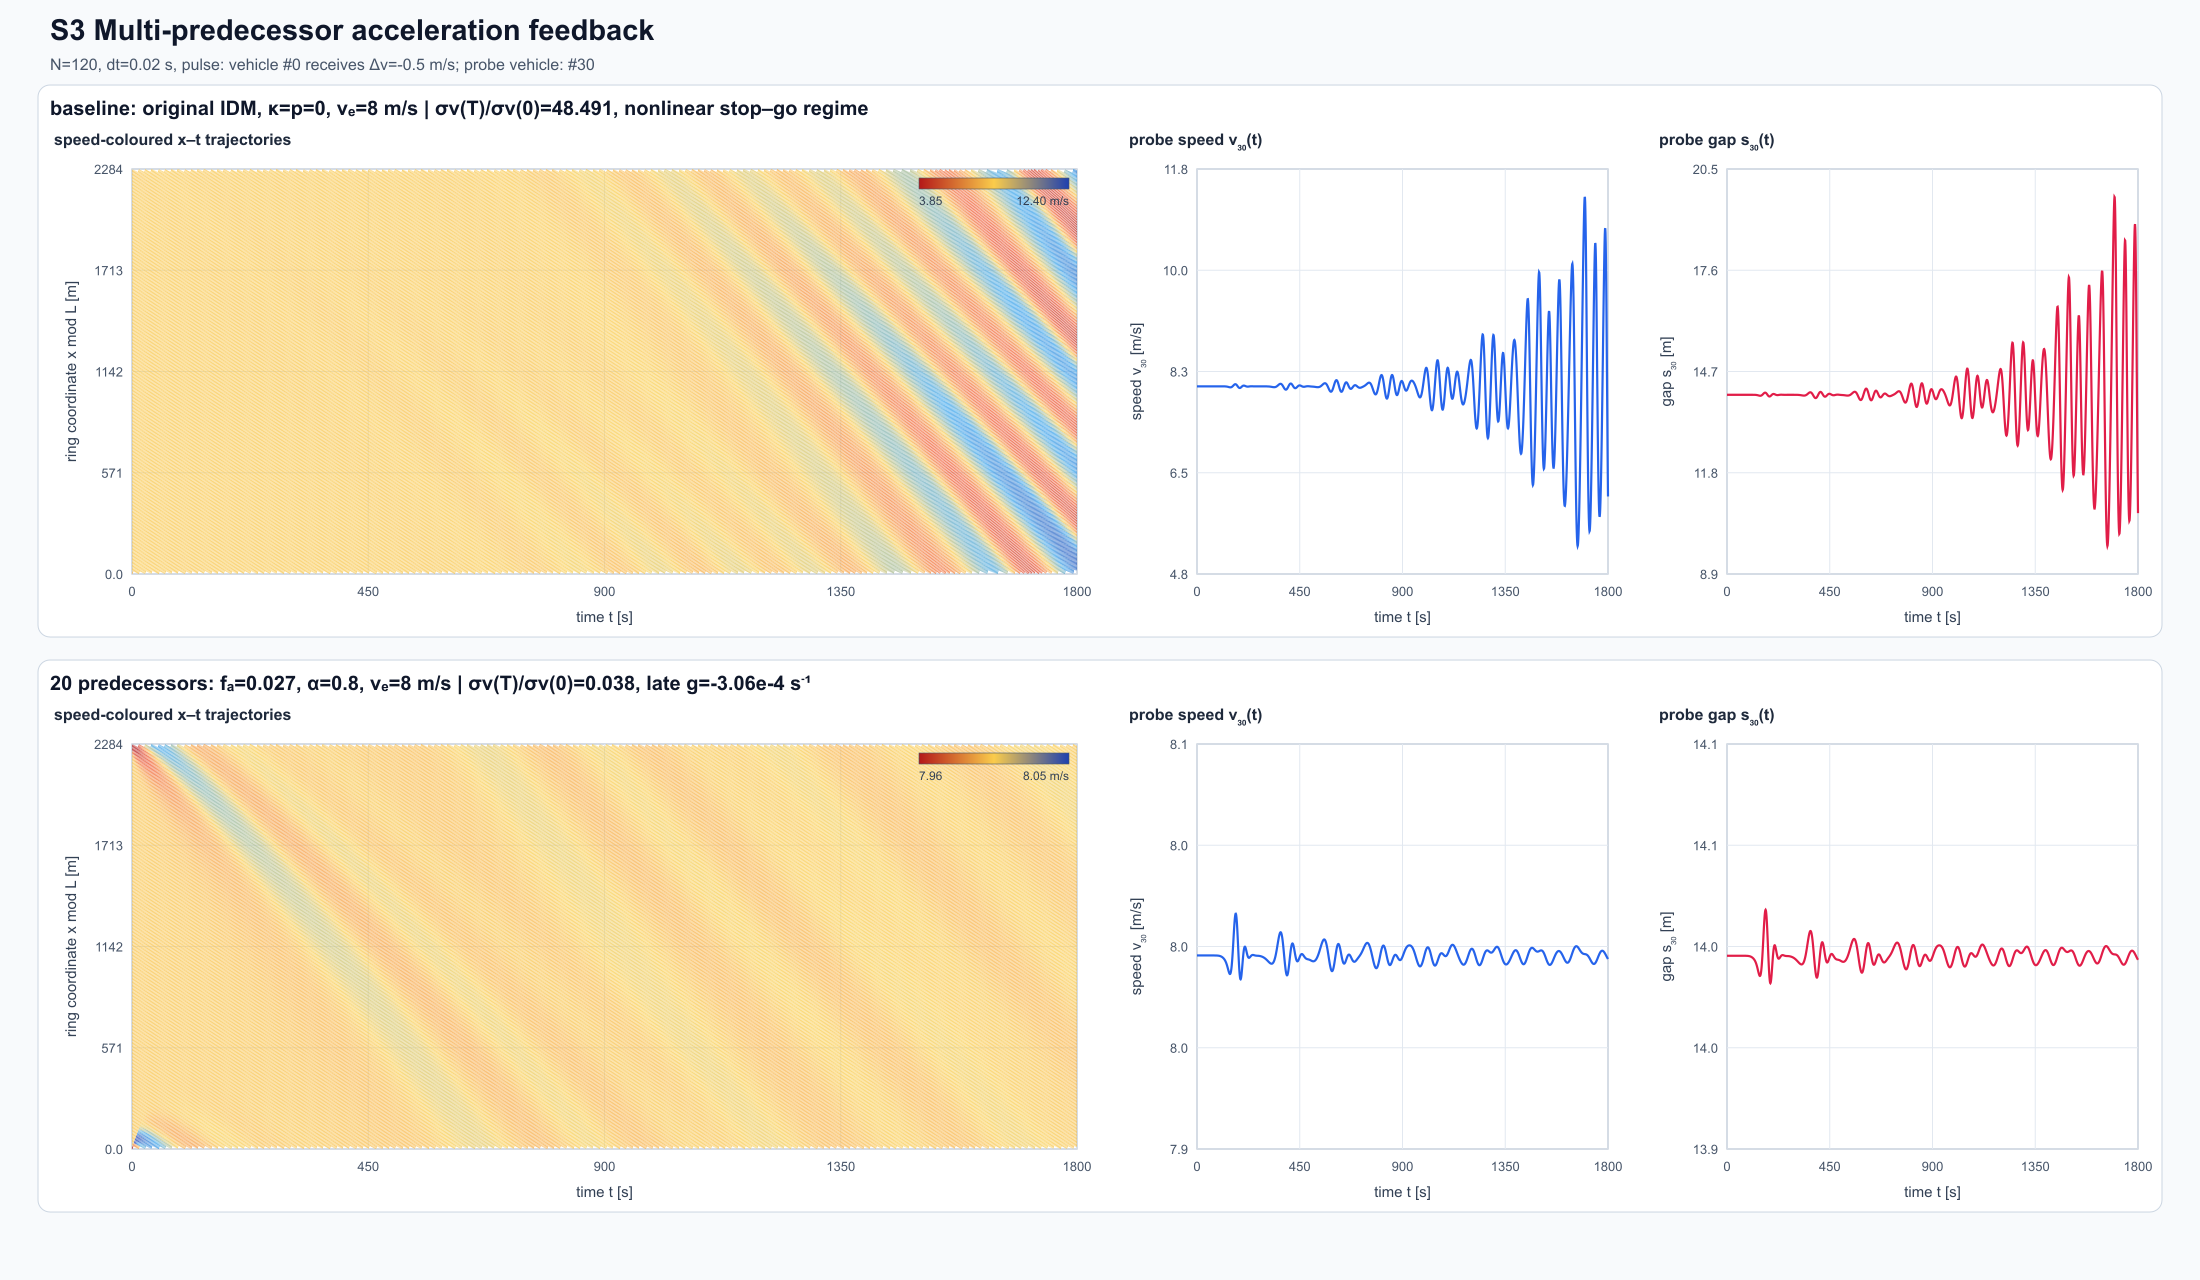
\includegraphics[width=\textwidth]{sim_s3_multi_front.png}
\caption{S3: Trajectory comparison based on feedback from multiple leading vehicles.}
\label{fig:traj-s3}
\figurenote{S3 transforms the multi-vehicle stability domain into observable traffic wave evolution. In the downlink, each vehicle receives the acceleration data of the 20 vehicles ahead, weighted with an exponential decay as defined by $\alpha=0.8$, with a nearest-neighbor coefficient of only $f_a=0.027$; the uplink continues to use the same instability threshold. Although the gain from a single nearest neighbor is far smaller than $0.15$ in S1, the total sum of the exponential kernels is approximately $f_a/(1-\alpha)$, which is sufficient to exceed the long-wave threshold; the downlink color bands fade with each lap, and the specified vehicle speeds and headways return to equilibrium, verifying that “the total sum can be distributed among multiple leading vehicles.” Compared to the stop-and-go waves formed during the upward phase, the downward phase did not exhibit new short-wave textures caused by long-range information, indicating that the selected attenuation kernel also passed the finite wavelength test. This figure demonstrates that the benefit of multi-vehicle forward communication does not lie in larger individual control actions, but rather in the collective contribution of smaller, spatially distributed gains to provide a stable budget.}
\end{figure}

\section{Why Are Forward and Rearview Perspectives So Asymmetrical?}
\sectionstudy{theory}{Why Are Forward and Rearview So Asymmetrical?}{lenz1999,feng2019}







\label{sub:asym}




There is a very straightforward explanation for the numerical differences above. Let’s break down $P$ using Euler’s formula:

\begin{equation}
P(k) = 1 - \sum_{j\ge1}\left(a_j e^{-ijk} + b_j e^{ijk}\right)
\end{equation}







\begin{tcolorbox}[keybox]
\begin{equation}
P_r = 1 - \sum_{j\ge1}\left(a_j+b_j\right)\cos jk,
\qquad
P_i = \sum_{j\ge1}\left(a_j-b_j\right)\sin jk
\end{equation}
\end{tcolorbox}

\textbf{$P_r$ considers only the symmetric part of the coupling kernel, while $P_i$ considers only the antisymmetric part.}




 Therefore: by switching the same gain from forward-looking to backward-looking, $P_r$




\textbf{Not a single character has changed}, only $P_i$ is reversed as a whole.




Now look at the coefficient of $P_i$ in Condition II:

\begin{equation}
\widetilde W \;\supset\; P_i\,s\underbrace{\Big[2f_sP_r + f_{v_l}\left(f_{v_l}-f_v\right)\Big]}_{\textstyle >\,0\ \text{always positive}}
\end{equation}

(Because of $f_v<0<f_{v_l}$, therefore $f_{v_l}-f_v>0$.) Therefore










\begin{tcolorbox}[notebox]
\textbf{Looking forward ($P_i>0$) adds points, while looking back ($P_i<0$) subtracts points, and the magnitudes are completely symmetrical.}




The only difference between the two is this single symbol.







\end{tcolorbox}

\subsection{Moment expansion: The advantage is the zero-order moment; the disadvantage is the first-order moment.}










Expand near $k\to0$ ($u=1-k^2/2$, $s=k$), and denote the moments of each order of the coupling kernel as

\begin{equation}
m_0 = \sum_j\left(a_j+b_j\right) = \sigma_{\rm eff},
\qquad
m_1 = \sum_j j\left(a_j-b_j\right),
\qquad
m_2 = \sum_j j^2\left(a_j+b_j\right)
\end{equation}

Then $P_r \approx \left(1-m_0\right) + \tfrac12 m_2k^2$ and $P_i\approx m_1k$; substituting yields

\begin{equation}
\widetilde W(k) \;\approx\; \underbrace{P_0\left(f_v^2-f_{v_l}^2-2f_sP_0\right)}_{\text{contains only  }m_0}
\;+\; k^2\Big\{\underbrace{m_1\left[2f_sP_0+f_{v_l}\left(f_{v_l}-f_v\right)\right]}_{\text{antisymmetric; its sign determines the outcome}} + \big(\text{contains only  }m_0,m_2\text{ terms}\big)\Big\}
\end{equation}

where $P_0=1-m_0$.










\begin{tcolorbox}[keybox,title=\textbf{Conclusion}]
\begin{itemize}[leftmargin=1.2em,itemsep=3pt]
\item \textbf{Advantage (relaxing the long-wave threshold): it depends only on the zero-order moment $m_0=\sigma_{\rm eff}$
}




, and is independent of the order of allocation;







\item \textbf{Disadvantage (the $k^2$ term is suppressed): it relies on first-order moments $m_1$}, with a positive forward-looking contribution and a negative backward-looking contribution.







\end{itemize}
\end{tcolorbox}










For the exponential decay kernel:

\begin{equation}
\sum_j j\,a_j = \frac{f_a}{\left(1-\alpha\right)^2} = \frac{\sigma_a}{1-\alpha},
\qquad
\sum_j j\,b_j = \frac{f_b}{\left(1-\beta\right)^2} = \frac{\sigma_b}{1-\beta}
\end{equation}

where $\sigma_a=f_a/(1-\alpha)$ and $\sigma_b=f_b/(1-\beta)$ are their respective total quantities, and $1/(1-\alpha)$ and $1/(1-\beta)$ are precisely




\textbf{the average observation distance}




(Unit: vehicles).










\begin{tcolorbox}[notebox,title=\textbf{This answers the question, “Why does looking back at a single vehicle work, but not at multiple vehicles?”}]

When the fixed total $\sigma_b$ remains constant:

\[
\text{zeroth moment (benefit)} = \sigma_b \ \text{unchanged},
\qquad
\text{first moment (cost)} = \frac{\sigma_b}{1-\beta}\ \text{amplified } \frac{1}{1-\beta}\ \text{ times}
\]







\textbf{Looking back at one vehicle}




($\beta=0$), the average distance is 1, resulting in the lowest penalty; the benefits of the zero-order moment prevail, yielding a positive net gain;




\textbf{When looking back at multiple vehicles}




the benefits do not increase at all, but the penalty points expand according to $1/(1-\beta)$, resulting in a negative net gain. In the forward-looking direction, the opposite is true—the farther the spread, the larger $m_1$ becomes, and the more the $k^2$ term is elevated, so spreading in any way is safe.







\end{tcolorbox}

\textbf{Numerical verification.} Retrieve $v_e=8$ m/s, $\sigma_{\rm eff}=0.3$, and the attenuation factor $0.85$ (i.e., the nearest-neighbor gain $0.045$):










\begin{center}
\captionof{table}{First-order moment effects for forward and backward views when the zero-order moment is fixed.}
\label{tab:first-moment-effect}
\begin{tabular}{lccc}
\toprule
& $m_1$ &




$k^2$ coefficient




& $\min_k\widetilde W$ \\
\midrule







Pure Forward View $\alpha=0.85$




& $+2.00$ & $-0.184$ &




$+0.029$ (Stable)



\\







Pure Look-Back $\beta=0.85$




& $-2.00$ & $-3.110$ &




 $-0.027$ (Unstable)



\\
\bottomrule
\end{tabular}
\end{center}
\tabletext{tab:first-moment-effect}{




For the same $m_0$, the coefficients and minimum margins of $m_1$ and $k^2$ for pure forward-looking and pure backward-looking scenarios, respectively. The difference between the two rows corresponds exactly to the first-order moment term, proving that the finite wavelength difference stems from directional phase rather than total gain.}





The $P_r$, $m_0$, and $m_2$ values for both are exactly the same, and $\widetilde W(0)$ is also the same as $+0.0333$; the difference in the coefficients of $k^2$ is exactly

\begin{equation}
2m_1\left[2f_sP_0+f_{v_l}\left(f_{v_l}-f_v\right)\right] = 2\times2.00\times0.732 = 2.93
\end{equation}

and exactly matches $-0.184-(-3.110)=2.93$ in the table.










\subsection{Physical image}










$\sin(jk)$ is precisely the number of vehicles separated by $j$




\textbf{Phase difference}




. Stop-and-go wave along the convoy




\textbf{backward}




through the convoy (from the leading car $\to$ to the current car $\to$ to the trailing car), therefore







\begin{itemize}[leftmargin=1.4em,itemsep=3pt]
\item




 $\dot v_{n-j}$ is a disturbance




\textbf{is about to reach itself}




preview information—phase lead; the further ahead you look, the greater the lead, the more advantageous it is;







\item




 $\dot v_{n+j}$ is a perturbation




\textbf{has already left itself}Subsequent feedback—phase lag—increases the further back you look, which is equivalent to introducing a longer delay into the loop, making it increasingly detrimental.







\end{itemize}







The closest following vehicle ($j=1$) exhibits the least lag; the benefit of its “total feedback” still outweighs the drawback of “phase lag.” However, this is no longer the case for vehicles further back.










\section{Negative Sign for Backward Look: A Common Convention in the Literature}
\sectionstudy{theory}{Negative Sign for Backward Look: A Common Convention in the Literature}{lenz1999,feng2019}
\label{sub:negfb}

\subsection{First, Verify the Notation Conventions}










The notation used in this book is $f_b = \partial f/\partial\dot v_{n+1}$; the numerical examples preceding it use $f_b>0$ by default. There are two common notations found in the literature, and the results differ completely when mapped to the notation used in this book. Be sure to verify the notation before applying it:










\begin{center}
\captionof{table}{Correspondence between the two types of rear-vehicle acceleration notations and the symbols used in this book.}
\label{tab:rear-acceleration-signs}
\begin{tabular}{p{6.4cm}p{4.2cm}p{3.4cm}}
\toprule







Notation in the literature




&




 Equivalent to $f_b$ in this book




&




 Symbol



\\
\midrule
$\dot v_n = F + \lambda_a\dot v_{n-1} - \lambda_b\dot v_{n+1}$ & $f_b = -\lambda_b$ & \textbf{Negative} 
\\[4pt]
$\dot v_n = F + \gamma_b\left(\dot v_{n+1}-\dot v_n\right)$ (relative acceleration)

&

$f_b = \dfrac{\gamma_b}{1+\gamma_b}$, and $f_s,f_v,f_{v_l}$ divided by $1+\gamma_b$

& \textbf{positive} \\
\bottomrule
\end{tabular}
\end{center}
\tabletext{tab:rear-acceleration-signs}{

The sign corresponding to the two formulations found in the literature—absolute acceleration of the following vehicle versus relative acceleration—when mapped to $f_b$. This comparison prevents equating the linguistic label "negative feedback" directly with the sign of the parameter used in this book.
}



If a paper treats the rear-looking term as

\textbf{negative feedback}

it corresponds to $f_b<0$ in this book.



\subsection{What a negative $f_b$ does within the moment framework}



Returning toThe two moments of $5\times10^{-2}$:
\begin{equation}
m_0 = \frac{f_a}{1-\alpha}+\frac{f_b}{1-\beta} = \sigma_{\rm eff},
\qquad
m_1 = \frac{f_a}{\left(1-\alpha\right)^2} - \frac{f_b}{\left(1-\beta\right)^2}
\end{equation}

At $f_b<0$, both change simultaneously but in opposite directions:



\begin{tcolorbox}[keybox,title=\textbf{Negative look-back = trading long-wave margin for finite-wavelength margin}]
\begin{itemize}[leftmargin=1.2em,itemsep=3pt]
\item $m_0$ \textbf{Decrease}

$\Rightarrow$ The long-wave condition $\tfrac12(f_v^2-f_{v_l}^2)\ge(1-m_0)f_s$ becomes tighter (unfavorable);


\item $m_1$ \textbf{Increase}

(Due to $-f_b/(1-\beta)^2>0$) the $\Rightarrow$ $k^2$ term is raised (favorable).


\end{itemize}


It is precisely the mirror image of the case at $f_b>0$.


\end{tcolorbox}



Thus, whether to choose positive or negative depends entirely on

\textbf{which side the bottleneck is on}

: If $\sigma_{\rm eff}$ is already insufficient (long-wave is the bottleneck), a positive $f_b$ must be used to supplement the total amount; if look-ahead has already boosted $\sigma_{\rm eff}$ sufficiently high and the bottleneck has shifted to finite wavelengths, then a negative $f_b$ should be used.



\subsection{Numerical example}

\begin{figure}[htbp]
\centering
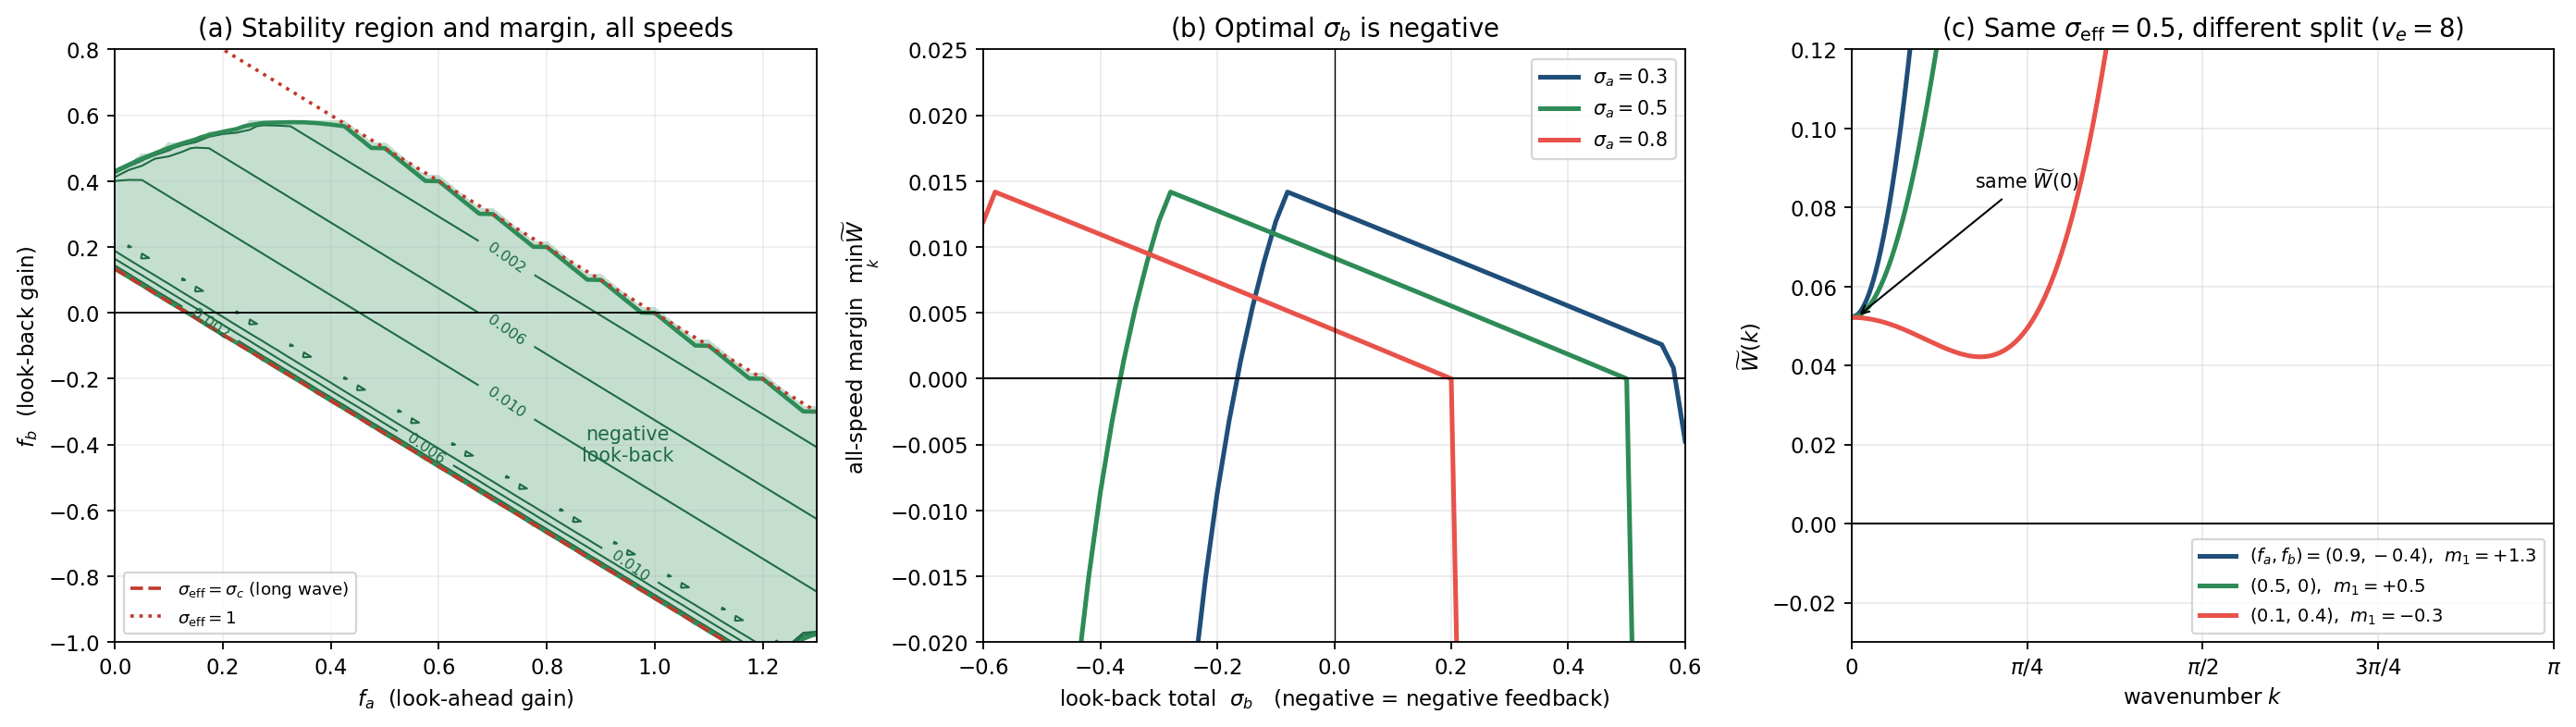
\includegraphics[width=\textwidth]{fig6.png}
\caption{Margins, optimal allocation, and moment effects based on feedback from multiple neighboring vehicles.}
\label{fig:moment-domain}
\figurenote{The stratified roles of feedback signs and spatial moments regarding stability across the full velocity range. The left panel projects the stability margin—evaluated at the worst-case operating point and wavenumber—onto the plane of forward-looking and backward-looking feedback gains; the boundary indicates that a moderate negative backward-looking gain can provide damping in conjunction with forward-looking feedback, whereas excessive gain introduces instability at finite wavelengths. The middle panel shows the effect of varying the backward-looking gain while keeping the total forward-looking gain constant; the local maxima within the curves demonstrate that neither "more backward-looking gain is better" nor "no backward-looking gain at all" holds as a general rule, as the optimal value arises from a balance between phase compensation and non-local side effects. The right panel maintains a constant zero-order moment while varying only the first-order moment of the kernel; the three curves coincide at the zero-order limit, demonstrating that the zero-order total determines the long-wave threshold, whereas they diverge at finite first-order moment values to exhibit distinct minima, proving that observation distance and direction govern the safety margins for medium- and short-wave modes. This figure refines the heuristic "forward-looking is good, backward-looking is bad" into quantifiable conditions: the zero-order moment determines whether the system clears the long-wave stability boundary, while the first-order moment determines whether instability re-emerges at finite wavelengths after crossing that boundary.}
\end{figure}

Three directly applicable conclusions:



\begin{itemize}[leftmargin=1.4em,itemsep=4pt]
\item \textbf{The in-band stability margin is determined almost exclusively by the zero-order moment.}

The contour lines in panel (a) are nearly parallel to the constant zero-order moment lines; provided the system is not operating close to the boundary, the specific allocation between forward- and backward-looking components has negligible impact on the magnitude of the margin, affecting only

\textbf{the position of the boundary.}。

\item \textbf{The true value of negative backward-looking feedback lies in relaxing the upper bound of the zero-order moment.}The hard constraint $\sigma_{\rm eff}<1$ directly limits $f_a<1$ when only look-ahead is used. If one wishes to increase $f_a$ to facilitate rapid following or maintain small spacing, a negative $f_b$ must be used to pull the total value back: in Figure (a), when $f_b=-0.4$, $f_a$ can be set above $1.3$ while remaining stable across the entire speed range.



\item \textbf{The optimal total value for the full speed range is approximately $\sigma_{\rm eff}\approx0.22$
}

(maximizing the minimum value of $P_0\left(f_v^2-f_{v_l}^2-2f_sP_0\right)$ across the full speed range, $P_0=1-\sigma_{\rm eff}$), corresponding to a margin of $0.0142$. At $\sigma_a=0.3/0.5/0.8$, the optimal $\sigma_b$ values are $-0.08/-0.28/-0.58$, respectively.


\end{itemize}

\subsection{The distribution direction also reverses accordingly}

$t=t_{\rm int}$ stated: backward distribution amplifies $|m_1|$ by a factor of $1/(1-\beta)$. When $f_b>0$, this amplification represents a

\textbf{penalty}

, and is therefore detrimental; when $f_b<0$, the amplification represents a

\textbf{bonus}, thus

\textbf{harmless or even beneficial}

. Numerically, when $\sigma_a=0.5$ and $\sigma_b=-0.3$ vary such that $\beta$ increases from $0$ to $0.9$, the margin across the entire speed range remains essentially unchanged (with only slight fluctuations); there is absolutely no occurrence of the collapse associated with the positive look-back case (where $\beta\gtrsim0.58$ leads to instability).



\begin{tcolorbox}[notebox,title=\textbf{Summary}]
The sign of $f_b$ determines the

\textbf{scale}

at which it provides assistance: a positive sign supplements the total long-wave magnitude, while a negative sign corrects the phase of finite-wavelength components. Literature often adopts the negative sign because, in those settings, the long-wave condition is already satisfied by the look-ahead term, making the phase margin of finite-wavelength components the actual bottleneck.


\end{tcolorbox}

\begin{tcolorbox}[notebox,title=\textbf{Engineering Conclusion}]
\begin{itemize}[leftmargin=1.2em,itemsep=3pt]
\item \textbf{The long-wave threshold is determined solely by the total magnitude.}

During design, the total gain budget can be determined first based on $\sigma_{\rm eff}\ge\sigma_c$, followed by a discussion on spatial allocation.


\item \textbf{Allocating gain to look-ahead vehicles does not reduce the long-wave margin.}

Distributing the same total magnitude across multiple leading vehicles allows for a linear reduction in nearest-neighbor gain while maintaining the long-wave condition—this represents the direct value of multi-vehicle look-ahead sensing (such as V2V broadcasting or multi-target radar).\item \textbf{Backward distribution comes at a cost (limited to $f_b>0$).}

Distributing positive look-back feedback to distant vehicles introduces instability in the short-wave range; $\beta$ should not exceed approximately $0.5$. However, if one adopts the

\textbf{negative}

look-back convention ($f_b<0$; see

$t\approx543$), this conclusion is reversed.


\item

Optimal configuration:

\textbf{Use a larger $\alpha$ for forward-looking feedback to dilute the gain, while limiting look-back feedback to only the nearest one or two vehicles with conservative gain settings.}。
\end{itemize}
\end{tcolorbox}

%==================================================================
\sectionwrapup{Multi-vehicle information is determined by the zero-order moment of the weighting kernel, spatial distribution, and directional asymmetry. The zero-order moment governs long-wave gain, whereas long-range look-back feedback can trigger new instabilities at specific wavelengths; therefore, the total gain should be allocated first, followed by a scan of the full wavenumber range.}

\chapter{Clarification: Most "rear-looking" feedback in the literature is not acceleration feedback.}
\label{sec:reargap}
\chapterguide{Why different studies on "rear-looking" feedback yield contradictory conclusions.}{

This chapter strictly distinguishes between three types of feedback channels—following-vehicle acceleration, backward headway, and backward relative velocity—and demonstrates that backward headway feedback alters not only the growth rate but also the long-wave propagation speed, thereby resolving the confusion between sign conventions and physical effects. }

Chapter ~\ref{sec:multi}~ The conclusion reached is: separate

\textbf{negative}Following vehicle

\textbf{Acceleration}

Feedback degrades stability. This appears to contradict the findings of numerous studies on "rearward-looking" behavior, which report that looking backward significantly improves stability. The root of this contradiction lies in

\textbf{Different feedback channels}。

\section{Two completely different types of "rearward-looking" behavior}
\sectionstudy{theory}{Two completely different types of "rearward-looking" behavior}{wilsonward2011,stuedli2017}

\begin{center}
\captionof{table}{The mechanistic difference between following-vehicle acceleration feedback and rearward spacing feedback.}
\label{tab:two-rear-looking-mechanisms}
\begin{tabular}{p{3.2cm}p{5.4cm}p{5.4cm}}
\toprule
& \textbf{Following-vehicle acceleration feedback (Chapter ~\ref{sec:lead}~ – Chapter ~\ref{sec:multi}~)
} & \textbf{Rearward spacing/relative velocity feedback (this chapter)} \\
\midrule


Feedback variable

& $\dot v_{n+1}$ & $s_{n+1}=x_n-x_{n+1}-l$，$\ v_{n+1}-v_n$ \\[4pt]
Which term is modified?

&

Only modify $P(k)$ (the coefficient of $\lambda^2$)

&

Modify $R(k)$ and $Q(k)$
\\[4pt]
Is the wave speed $c_1$ changed?

&

No

& \textbf{Yes} \\[4pt]
Typical source&CACC feedforward/communication-based models

&

Look-back OVM, bilateral control
\\
\bottomrule
\end{tabular}
\end{center}
\tabletext{tab:two-rear-looking-mechanisms}{

Regarding the two types of "look-back" feedback: their input variables, their points of entry into the characteristic equation, and whether they alter wave speed. Conclusions in the literature may appear contradictory, but this is often simply because different feedback channels were investigated.
}

The vast majority of "look-back" car-following models belong to

\textbf{the second category}

. For instance, expressing the optimal velocity function as
\[
(1-p)V_F(s_n)+pV_B(s_{n+1}),\qquad V_B'<0.
\]





The term “negative feedback” refers to the fact that




\textbf{rear distance}




—the closer the vehicle behind gets, the more the leading vehicle accelerates—rather than taking the negative of the rear vehicle’s acceleration.










\section{Linearization and Characteristic Equation}
\sectionstudy{model}{Linearization and Characteristic Equations}{wilsonward2011,stuedli2017}










Let the backward distance gain be $h_s = -\partial G/\partial s_{n+1} > 0$ and the backward relative velocity gain be $h_v>0$, then

\begin{equation}
\ddot y_n = f_s\left(y_{n-1}-y_n\right) + h_s\left(y_{n+1}-y_n\right)
+ f_v\dot y_n + f_{v_l}\dot y_{n-1} + h_v\left(\dot y_{n+1}-\dot y_n\right)
\end{equation}




Note that the distance term is now a




\textbf{discrete Laplacian}




—the vehicle is “pulled” simultaneously from both the front and rear, which is precisely the core of bidirectional control. After the Fourier transform:







\begin{tcolorbox}[keybox]
\begin{equation}
\lambda^2 - \underbrace{\left[f_v-h_v+f_{v_l}e^{-ik}+h_ve^{ik}\right]}_{Q(k)}\lambda
- \underbrace{\left[f_s\left(e^{-ik}-1\right)+h_s\left(e^{ik}-1\right)\right]}_{R(k)} = 0
\end{equation}
\end{tcolorbox}










Key difference: The coefficients of $\lambda^2$ remain $1$ ($P\equiv1$),




\textbf{while $Q$ and $R$ have changed}




. This is precisely complementary to Chapters ~\ref{sec:lead}~ through ~\ref{sec:multi}~.










\section{The wave velocity has been changed—that is the key point}
\sectionstudy{theory}{The wave velocity is altered—this is the key}{wilsonward2011,stuedli2017}










The $O(\varepsilon)$th-order expansion of the long wave is now given







\begin{tcolorbox}[keybox]
\begin{equation}
c_1 = -\frac{f_s-h_s}{f_v+f_{v_l}} = \left(1-\frac{h_s}{f_s}\right)V'(s_e)
\end{equation}
\end{tcolorbox}

\textbf{Backward spacing feedback directly reduces the kinematic wave velocity}, and in the limit of perfect symmetry $h_s=f_s$, $c_1=0$, at which point the long-wave phase no longer propagates in the direction of the vehicle serial number. It should be noted that this limit is not the same concept as “just reaching the linear stability threshold”; the reference case has already achieved linear stability across the entire speed range at $p_c=0.223$, but the wave speed at this point is still $(1-p_c)V'$. Acceleration feedback does not alter $c_1$ ($c_1=V'$ is present throughout Chapters ~\ref{sec:lead}~–~\ref{sec:multi}~).




The $O(\varepsilon^2)$th order yields (denoted as $\mu=f_v+f_{v_l}<0$)

\begin{equation}
\left(f_s-h_s\right)^2 + \mu\left(f_{v_l}-h_v\right)\left(f_s-h_s\right) - \frac{\mu^2\left(f_s+h_s\right)}{2} \;\le\; 0
\end{equation}




Taking $h_s=h_v=0$ reduces to $\tfrac12(f_v^2-f_{v_l}^2)\ge f_s$, which is self-consistent.










\section{Closed-form results under symmetric weights}
\sectionstudy{theory}{Closed-form results under symmetric weights}{wilsonward2011,stuedli2017}










Taking the common proportional forms $h_s=p\,f_s$ and $h_v=p\,f_{v_l}$ ($p\in[0,1]$ represents the rear-view weight), the conditions are










\begin{tcolorbox}[keybox,title=\textbf{Linear stability conditions for the rear-view weight $p$}]

\begin{equation}
\underbrace{\frac{2\left(f_s+\mu f_{v_l}\right)}{\mu^2}}_{\textstyle \text{depends only on the original model}}
\;\le\;
\frac{1+p}{\left(1-p\right)^2}
\end{equation}

The threshold value at the left end, $p=0$, is $1$, which is the original criterion; the right end is




\textbf{Relaxation factor}




, which increases rapidly with $p$.







\end{tcolorbox}










The relaxation factor increases rapidly: it is $1.88$ at $p=0.2$, $2.65$ at $p=0.3$, and $6$ at $p=0.5$. This is the mathematical reason behind the “significant effect” of the back-view—it does not linearly add a small margin, but rather expands the right end of the criterion




\textbf{by $(1-p)^{-2}$
}。

\section{IDM value}
\sectionstudy{model}{IDM value}{treiber2000,treiberkesting2013}










For the parameters in Chapter ~\ref{sec:num}~, the most severe point across the entire speed range is $\max_{v_e} 2\left(f_s+\mu f_{v_l}\right)/\mu^2 = 2.03$; therefore, the critical rearward weighting

\begin{equation}
p_c = 0.223
\end{equation}










\begin{center}
\captionof{table}{Rearward weighting for the narrowing of the IDM unstable speed band.}
\label{tab:rear-gap-band}
\begin{tabular}{rcc}
\toprule
$p$ &




Unstable speed band [m/s]




&




Relaxation factor



\\
\midrule
0.00 & $0.93$ -- $18.59$ & 1.00 \\
0.10 & $3.90$ -- $17.36$ & 1.36 \\
0.20 & $8.77$ -- $14.59$ & 1.88 \\
0.223 &




Critical& 2.03 \\
0.30 & Stability Across the Entire Speed Range




& 2.65 \\
\bottomrule
\end{tabular}
\end{center}
\tabletext{tab:rear-gap-band}{




Changes in the instability band and relaxation factor as the rear-view weight increases from 0 to 0.30. The speed band contracts from both ends and closes at $p_c=0.223$; the numerical changes are consistent with the analytical relaxation factor.
}










Note that the instability zone




\textbf{contracts from both ends toward the center}




and then disappears, rather than simply raising one side as in the case of acceleration feedback.










\begin{figure}[htbp]
\centering
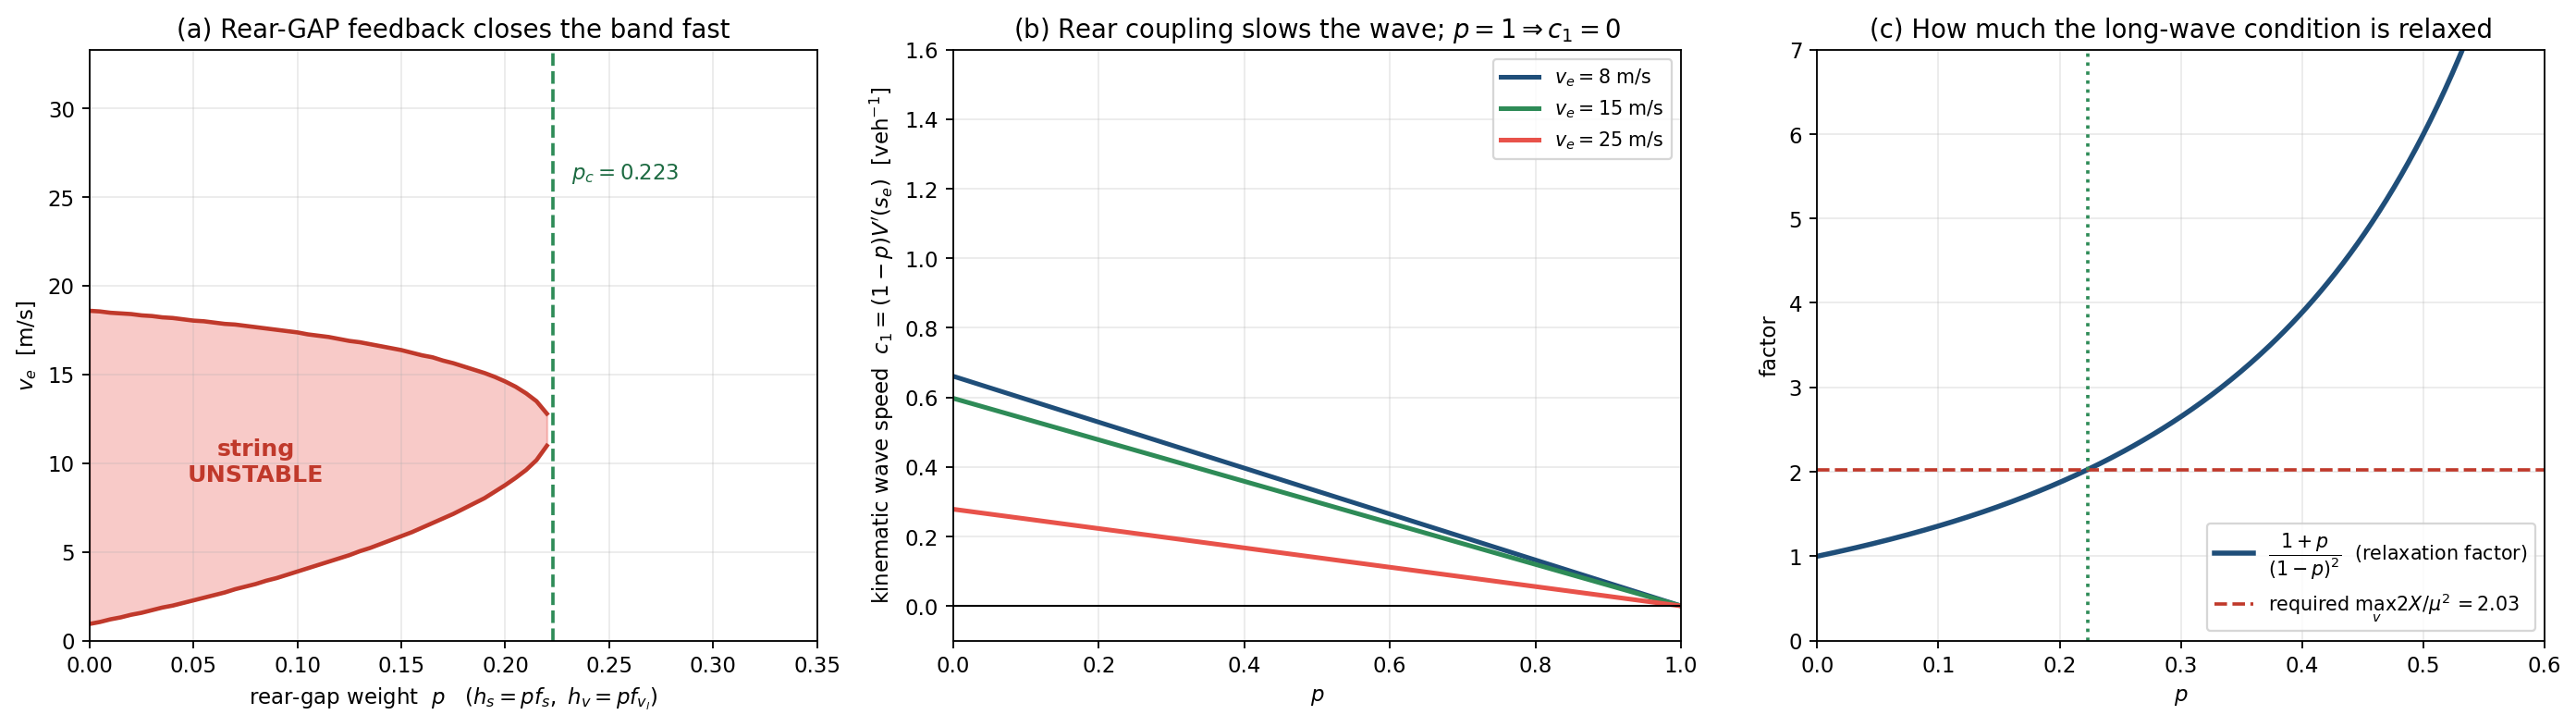
\includegraphics[width=\textwidth]{fig7.png}
\caption{Stability band and wave speed for backward spacing feedback.}
\label{fig:rear-gap-map}
\figurenote{Triple evidence that backward spacing/relative velocity feedback simultaneously alters both the stability region and the propagation speed. The left figure scans the long-wave margin on the velocity–weight plane; the instability band of the original IDM contracts from both ends as $p$ increases and completely closes at $p_c=0.223$; this provides a direct answer to the question of “how much backward weight is required.” The middle figure plots $c_1=(1-p)V'(s_e)$, showing that the same feedback reduces the kinematic wave speed while suppressing growth; consequently, the slope of the color bands in the spatiotemporal trajectories should also change. The right figure plots, respectively, the degree of instability that the baseline model needs to compensate for and the relaxation factor introduced by the backward-looking term; the points where the two curves touch or intersect verify $p_c$, ensuring that the critical values are not derived solely from numerical shading. Together, these three figures demonstrate that backward-looking spacing feedback does not merely increase damping: it modifies the convection term of the equilibrium perturbation, thereby determining both whether a wave will grow and how fast it will propagate.}
\end{figure}

\begin{tcolorbox}[notebox,title=\textbf{Returning to that question}]

The statement in the literature that “negative rearward feedback improves stability” is correct, and the conclusion in Chapter ~\ref{sec:multi}~ is also correct—but the two are referring to entirely different feedback variables:







\begin{itemize}[leftmargin=1.2em,itemsep=3pt]
\item \textbf{Rear-to-front distance / relative velocity}




When the feedback is applied to $Q,R$, it can both alter the wave speed $c_1$ and increase the stability margin; in the fully symmetric limit, it can achieve $c_1\to0$. In this example, achieving stability across the entire speed range requires only $p\ge0.223$, but reducing the wave speed to zero still requires $p\to1$;







\item \textbf{Rear Vehicle Acceleration}




Feedback enters only $P$ and does not alter $c_1$; it adjusts the stability margin via the zero-order moment $m_0$ and the first-order moment $m_1$, and when negative, it also reduces $m_0$.







\end{itemize}







Therefore:




\textbf{If the paper’s rearview term acts on the distance or speed, setting it to “negative” ($V_B'<0$) does indeed provide strong stability; if it is indeed a rear-vehicle acceleration term, then setting it to negative alone will result in poorer performance.}




Before applying the conclusion, first confirm what the independent variable of that term is.







\end{tcolorbox}

\section{Numerical verification of E9/E10: Closure of the stability band and decrease in wave speed}
\sectionstudy{experiment}{Numerical Validation E9/E10: Closure of the Stability Band and Decrease in Wave Velocity}{wilsonward2011,stuedli2017}










E9 performs a two-dimensional scan of $p\in[0,0.4]$ and $v_e\in(0,v_0)$ to record the instability band width; E10: Fix $v_e=8$ m/s and $N=120$, and measure the wave velocity based on the slope of the lowest modal phase.










\begin{center}
\small
\captionof{table}{Analytical vs. Numerical Comparison of the Stability Band and Wave Velocity Following E9/E10.}
\label{tab:e9e10-rear-gap}
\begin{tabular}{p{3.2cm}p{4.3cm}p{4.3cm}p{2.0cm}}
\toprule
\textbf{Measurements} & \textbf{Analytical Predictions} & \textbf{Numerical Results} & \textbf{Conclusion} \\
\midrule







Closure Weight




& $p_c=0.223$ &




 2D scan closed at $p\approx0.223$




&




 Consistent




\\[3pt]
$p=0.223$ Rightmost root

&

Should lie on the critical side of the left half-plane

& $-1.2747\times10^{-4}$ s$^{-1}$ &

Finite-ring stability
\\[3pt]
Long-wave speed

& $(1-p)V'=0.5128$ veh/s & $|\operatorname{Im}\lambda|/k=0.5114$ veh/s &

Error $0.27\%$
\\
\bottomrule
\end{tabular}
\end{center}
\tabletext{tab:e9e10-rear-gap}{

Analytical predictions and numerical results regarding critical weight, the rightmost root in a finite ring, and long-wave speed. It also confirms that backward headway feedback can alter stability margins and propagation speeds.
}

\begin{tcolorbox}[resultbox,title=\textbf{Verification of conclusions}]
Backward headway feedback simultaneously achieves two things: it shrinks the unstable region from both ends toward the center and reduces the propagation speed of stop-and-go waves by $1-p$. The slight difference between the measured $0.5114$ veh/s (at finite $k=2\pi/N$) and the long-wave limit of $0.5128$ veh/s is attributable to finite-wavelength corrections. This change in wave speed can be used to experimentally distinguish between S4 and S2: acceleration look-back can alter the growth rate but does not change $c_1$.


\end{tcolorbox}

\section{Specific trajectory results: backward headway and relative velocity feedback}
\sectionstudy{experiment}{Specific trajectory results: backward headway and relative velocity feedback}{ngsim2016,thiemann2008,krajewski2018}Figure ~\ref{fig:traj-s4} compares $p=0$ and $p=0.30>p_c$ at $v_e=8$ m/s. After incorporating backward spacing feedback, $\sigma_v(1800)/\sigma_v(0)$ decreases from $48.49$ to $0.00843$, with a terminal slope of $-5.16\times10^{-4}$ s$^{-1}$; the speed range for the 30th vehicle contracts to $7.9961$–$8.0041$ m/s, and the spacing range contracts to $14.0269$–$14.0446$ m. The trajectory band not only attenuates, but its propagation slope also differs from the baseline, corresponding to a reduction in wave speed $c_1=(1-p)V'$.



\begin{figure}[htbp]
\centering
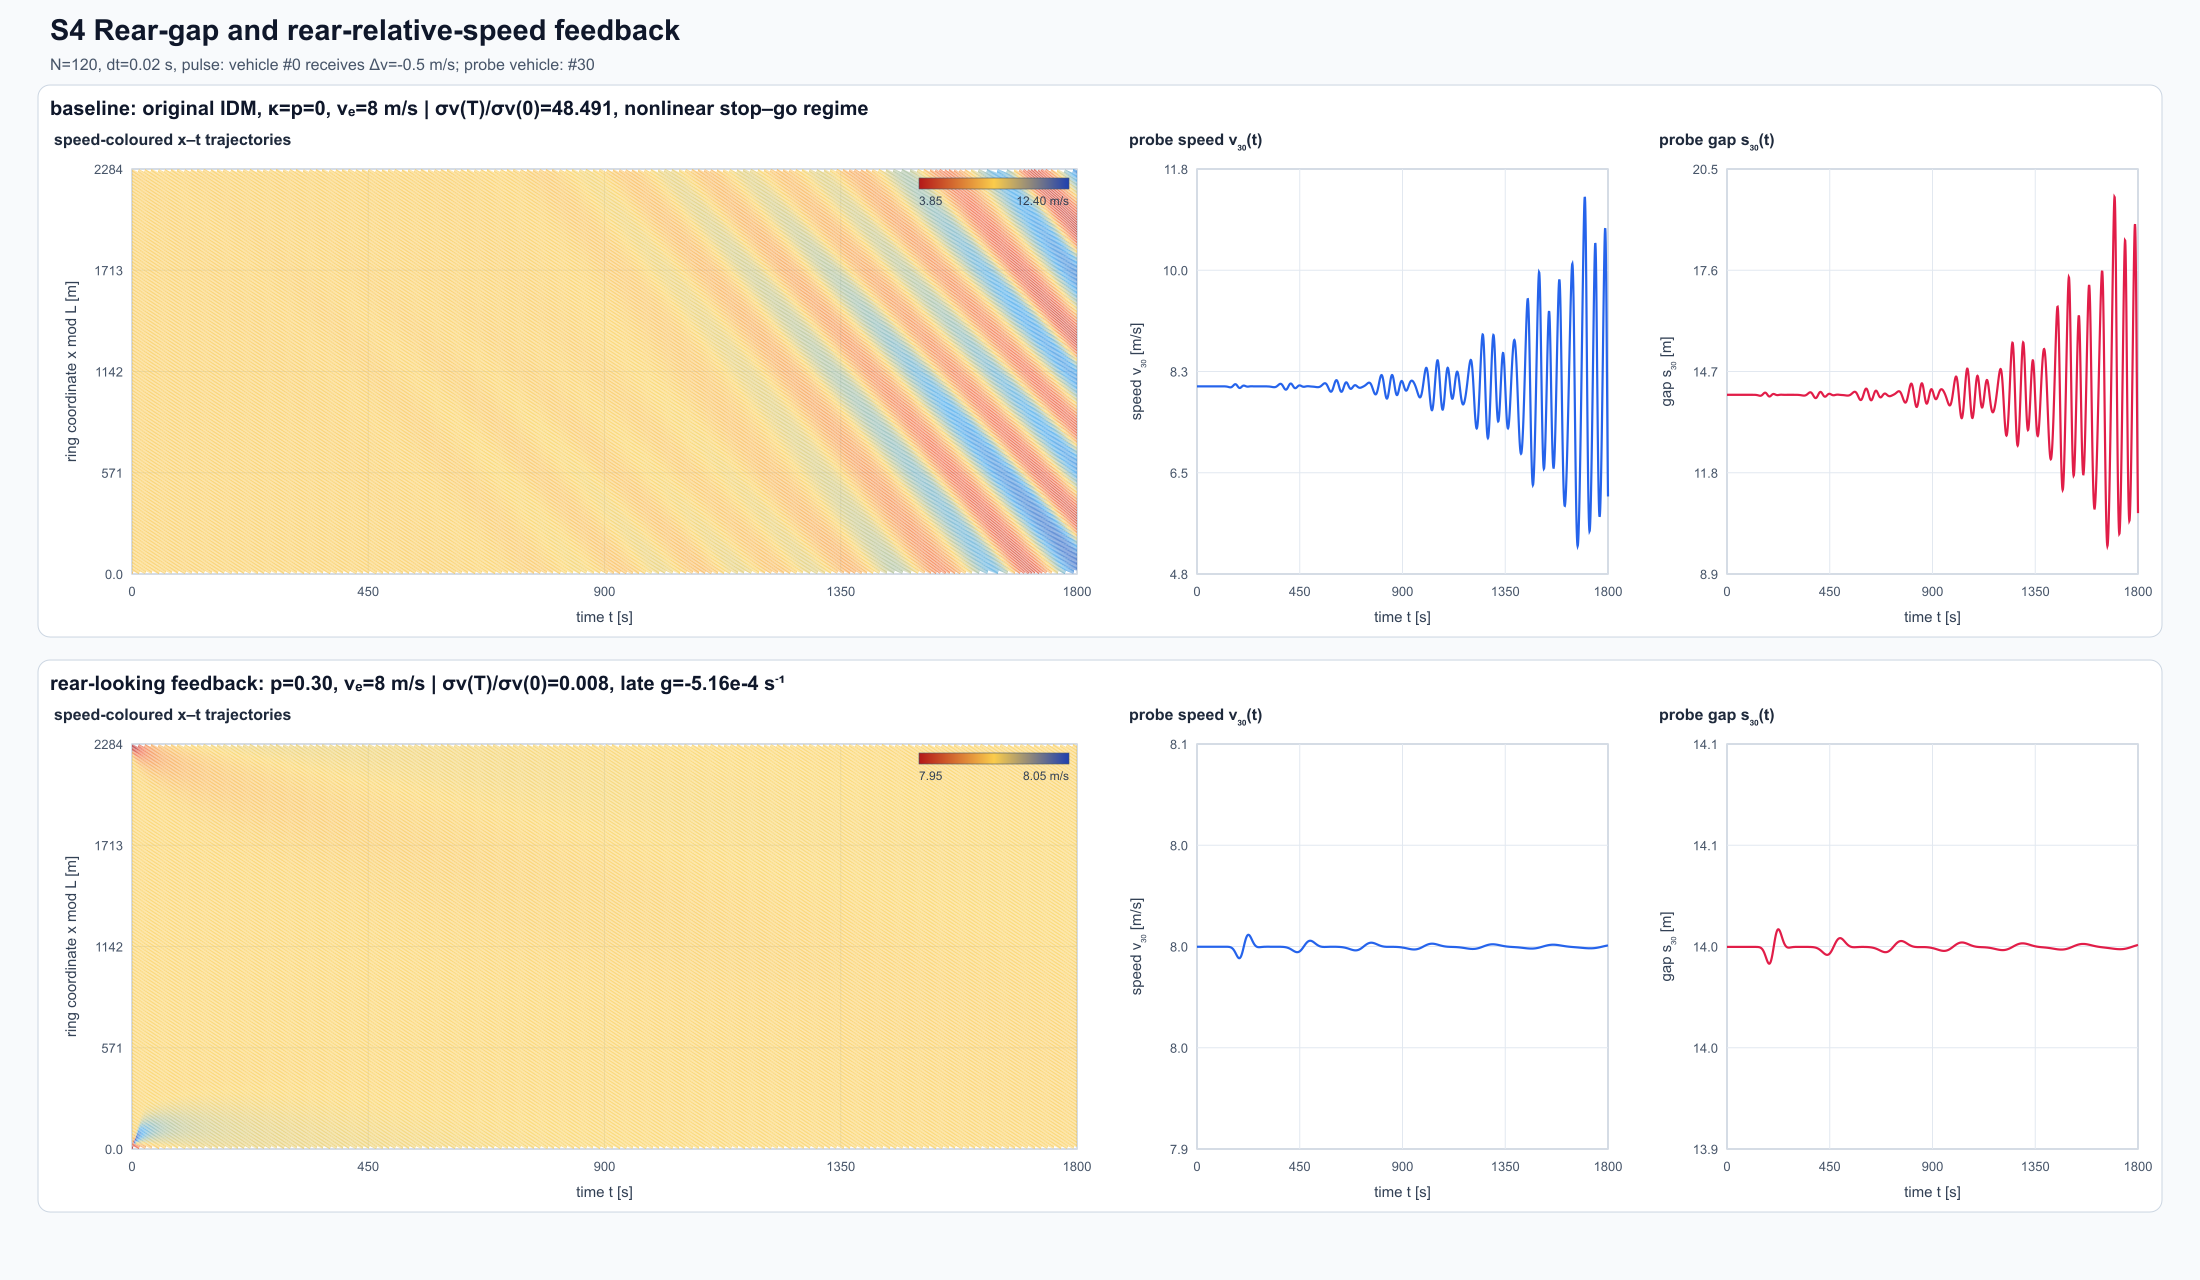
\includegraphics[width=\textwidth]{sim_s4_rear_gap.png}
\caption{S4: Comparison of trajectories with backward spacing feedback.}
\label{fig:traj-s4}
\figurenote{S4 Nonlinear time-domain verification of the analytical conclusions regarding backward headway feedback. The top and bottom rows correspond to $p=0$ and $p=0.30>p_c$, respectively, while all other operating points, initial pulses, and color scales remain identical; the top row exhibits a continuously intensifying stop-and-go wave, whereas the low-speed color band in the bottom row fades significantly within a few cycles. Beyond amplitude attenuation, the slope of the color band in the position-time plane differs from that of the top row, reflecting the reduction in $c_1$ predicted in Fig. \ref{fig:rear-gap-map}—evidence that cannot be obtained by observing probe amplitude alone. The velocity and net headway of the probe on the right return to equilibrium together, ruling out a state of "pseudo-stability" characterized by smooth velocity but drifting headway. This figure thus demonstrates that backward headway feedback stabilizes traffic flow by altering position recovery and wave speed—a mechanism distinct from follower acceleration feedback, which affects only the $\lambda^2$ coefficient.
}
\end{figure}

%==================================================================
\sectionwrapup{Follower acceleration feedback and backward headway/relative velocity feedback operate through different channels: the former primarily alters the growth rate, whereas the latter also modifies the propagation speed of long waves. Once sign conventions and feedback variables are clearly defined, the notion found in the literature that "rearward observation improves stability" is not inconsistent with the conclusions drawn here.}

\PART{V}{Breaking the polynomial nature: Time delay}

\chapter{Further generalization: Time delay in acceleration transmission}
\label{sec:delay}
\chapterguide{Why time delay leaves the static threshold unchanged yet can create new unstable frequency bands}{

This chapter establishes local and string stability conditions using quasipolynomials and transfer functions incorporating time delays. Readers should be able to distinguish between the long-wave limit, finite-frequency phase margin, and the infinite root spectrum, and understand when numerical root-finding must replace finite-dimensional stability criteria.
}

\section{Model}
\sectionstudy{model}{Model}{ororsz2004,ororsz2010}In practice, there are at least two types of delays: the driver's (or sensor's)

\textbf{perception-reaction delay}

$\tau_0$, and V2V

\textbf{communication delay}

$\tau_a,\tau_b$. Added to the corresponding terms respectively:
\begin{equation}
\dot v_n(t) = F\Big(s_n(t-\tau_0),\,v_n(t-\tau_0),\,\dv_n(t-\tau_0)\Big)
+ f_a\,\dot v_{n-1}(t-\tau_a) + f_b\,\dot v_{n+1}(t-\tau_b)
\end{equation}

After linearization:
\begin{equation}
\ddot y_n(t) = f_s\Big(y_{n-1}(t{-}\tau_0)-y_n(t{-}\tau_0)\Big) + f_v\dot y_n(t{-}\tau_0) + f_{v_l}\dot y_{n-1}(t{-}\tau_0)
+ f_a\ddot y_{n-1}(t{-}\tau_a) + f_b\ddot y_{n+1}(t{-}\tau_b)
\end{equation}



\section{The characteristic equation becomes a transcendental equation}
\sectionstudy{model}{The characteristic equation becomes a transcendental equation}{ororsz2004,ororsz2010}



Substituting $y_n=\hat y\,e^{\lambda t+ikn}$, noting the time-delay factor $e^{-\lambda\tau}$:


\begin{tcolorbox}[keybox]
\begin{equation}
\lambda^2\Big[1 - f_a e^{-\lambda\tau_a - ik} - f_b e^{-\lambda\tau_b + ik}\Big]
- e^{-\lambda\tau_0}\Big[\left(f_v + f_{v_l}e^{-ik}\right)\lambda + f_s\left(e^{-ik}-1\right)\Big] = 0
\end{equation}
\end{tcolorbox}

\begin{tcolorbox}[notebox,title=\textbf{Structural change}]
This is a

\textbf{quasi-polynomial}

(quasi-polynomial); it is no longer a finite-degree algebraic equation and has

\textbf{infinitely many roots}

. The Routh-Hurwitz and Bilharz criteria

\textbf{are no longer applicable}

. Available methods include: long-wave expansion, frequency-axis scanning (D-subdivision), and numerical pseudospectral discretization.


\end{tcolorbox}

\section{Local stability: now constrained by delay}
\sectionstudy{theory}{Local stability: now constrained by delay}{wilsonward2011,ororsz2010}



With the neighboring vehicle "frozen" (fixed relative to the ego vehicle), the acceleration coupling term vanishes, but the response delay remains:
\begin{equation}
\lambda^2 + e^{-\lambda\tau_0}\left(f_s - f_v\lambda\right) = 0
\end{equation}

Setting $\lambda=i\omega$ to find the neutral stability boundary:
\begin{equation}
e^{-i\omega\tau_0} = \frac{\omega^2}{f_s - i f_v\omega}
\end{equation}

Taking the magnitude yields $\omega^4 = f_s^2+f_v^2\omega^2$, and taking the argument yields $\omega\tau_0 = \arctan\!\big(\left|f_v\right|\omega/f_s\big)$; thus,



\begin{tcolorbox}[keybox,title=\textbf{Upper limit of delay for local stability}]
\begin{equation}
\omega_c = \sqrt{\frac{f_v^2 + \sqrt{f_v^4+4f_s^2}}{2}},
\qquad
\tau_0 \;<\; \tau_0^{\rm crit} = \frac{1}{\omega_c}\arctan\!\left(\frac{\left|f_v\right|\omega_c}{f_s}\right)
\end{equation}
\end{tcolorbox}



At $\tau_0=0$, it degenerates to the original $f_v<0,f_s>0$ (where $\tau_0^{\rm crit}>0$ holds true). For the IDM parameters in Chapter \ref{sec:num}:



\begin{center}
\captionof{table}{Upper limits of local response delay for three IDM operating points.}
\label{tab:local-delay-limits}
\begin{tabular}{rccc}
\toprule
$v_e$ [m/s] & 2 & 8 & 20 \\
\midrule
$\omega_c$ [rad/s] & 1.008 & 0.709 & 0.559 \\
$\tau_0^{\rm crit}$ [s] & 1.16 & 1.81 & 2.52 \\
\bottomrule
\end{tabular}
\end{center}
\tabletext{tab:local-delay-limits}{

Critical frequencies and upper limits of local response delay at different equilibrium speeds. Changes in the operating point alter the restoring stiffness and damping; therefore, the permissible delay cannot be represented by a single constant across the entire speed range.
}

\section{Long-wave condition: delay has no effect}
\sectionstudy{theory}{Long-wave condition: delay has no effect}{ororsz2004,ororsz2010}\label{sub:delaylw}

This is the most notable conclusion of this section. Let $\varepsilon=-ik$ and $\lambda=c_1\varepsilon+c_2\varepsilon^2+\cdots$ remain as defined. Since $\lambda=O(\varepsilon)$,
\begin{equation}
e^{-\lambda\tau} = 1 - c_1\tau\,\varepsilon + O(\varepsilon^2)
\end{equation}

We write the equation as $\lambda^2 M = e^{-\lambda\tau_0}N$, where
\begin{equation}
N = \left(f_v+f_{v_l}e^{\varepsilon}\right)\lambda + f_s\left(e^{\varepsilon}-1\right)
= \underbrace{\left[\left(f_v+f_{v_l}\right)c_1+f_s\right]}_{\textstyle =\,0}\varepsilon
+ \left[\left(f_v+f_{v_l}\right)c_2 + f_{v_l}c_1 + \frac{f_s}{2}\right]\varepsilon^2 + O(\varepsilon^3)
\end{equation}



\begin{tcolorbox}[notebox,title=\textbf{A crucial step}]
The first-order correction $-c_1\tau_0\varepsilon$ to $e^{-\lambda\tau_0}$ must be multiplied by the $O(\varepsilon)$ coefficient of $N$ to contribute to $O(\varepsilon^2)$—

\textbf{but that coefficient is exactly zero}

(it is precisely the equation that determines $c_1$). Therefore, $\tau_0$ is completely "absorbed" at order $O(\varepsilon^2)$. Similarly, the retardation correction in $M$ is $O(\varepsilon)$; multiplying it by $\lambda^2=O(\varepsilon^2)$ yields a result only at order $O(\varepsilon^3)$.


\end{tcolorbox}



Thus, $c_1=V'(s_e)$ and
\begin{equation}
\left(1-f_a-f_b\right)c_1^2 = \frac{f_s}{2} + f_{v_l}c_1 + \left(f_v+f_{v_l}\right)c_2
\end{equation}
are both identical, word for word, to the cases

\textbf{without retardation}：

\begin{tcolorbox}[keybox,title=\textbf{Long-wave condition (including arbitrary delay)}]
\begin{equation}
\frac{1}{2}\left(f_v^2-f_{v_l}^2\right) \;\ge\; \left(1-f_a-f_b\right)f_s
\end{equation}
\textbf{Entirely independent of $\tau_0,\tau_a,\tau_b$.}
\end{tcolorbox}



The physical meaning is straightforward: $k\to0$ implies $\lambda\to0$—meaning the perturbation changes very slowly, and for the delay element $e^{-\lambda\tau}\to1$, the phase lag is negligible.

\textbf{The disruptive effect of the delay manifests only at finite frequencies.}

—This is the same type of phenomenon as that described in Chapter \ref{sec:lead}, Section $f_a>1$.



\section{Finite-frequency condition: exact criterion for the unidirectional case}
\sectionstudy{theory}{Finite-frequency condition: exact criterion for the unidirectional case}{ororsz2004,ororsz2010}



For the unidirectional model ($f_b=0$), a transfer function can still be isolated after the Laplace transform:


\begin{tcolorbox}[keybox]
\begin{equation}
G(\lambda) = \frac{e^{-\lambda\tau_0}\left(f_s+f_{v_l}\lambda\right) + f_a\lambda^2 e^{-\lambda\tau_a}}
{\lambda^2 + e^{-\lambda\tau_0}\left(f_s - f_v\lambda\right)}
\end{equation}
\end{tcolorbox}



It is no longer a rational function, but

\textbf{the form of the criterion remains unchanged.}: $\left\|G\right\|_\infty\le1$, and the denominator has no zeros in the right half-plane (i.e., $\tau_0<\tau_0^{\rm crit}$).

Substituting $\lambda=i\omega$, let $\theta_0=\omega\tau_0$ and $\phi=\omega(\tau_a-\tau_0)$. Using $\left|e^{-i\theta}\right|=1$:
\begin{align}
\left|N\right|^2 &= f_s^2+f_{v_l}^2\omega^2 + f_a^2\omega^4
- 2f_a\omega^2\left[f_s\cos\phi - f_{v_l}\omega\sin\phi\right] \\
\left|D\right|^2 &= \omega^4 + f_s^2 + f_v^2\omega^2
- 2\omega^2\left[f_s\cos\theta_0 - f_v\omega\sin\theta_0\right]
\end{align}

Taking the difference and canceling the common factor $\omega^2$:



\begin{tcolorbox}[keybox,title=\textbf{String stability criterion with delay}]
\begin{align}
\Psi(\omega) = \;& \left(1-f_a^2\right)\omega^2 + f_v^2 - f_{v_l}^2 \nonumber\\
& - 2f_s\cos\!\left(\omega\tau_0\right) + 2f_v\,\omega\sin\!\left(\omega\tau_0\right) \nonumber\\
& + 2f_af_s\cos\!\left(\omega(\tau_a{-}\tau_0)\right) - 2f_af_{v_l}\,\omega\sin\!\left(\omega(\tau_a{-}\tau_0)\right)
\;\ge\; 0
\qquad \forall\,\omega\ge0
\label{eq:Psi}
\end{align}
\end{tcolorbox}

\textbf{Consistency check.}

Let $\tau_0=\tau_a=0$; then equation \eqref{eq:Psi} reduces to $(1-f_a^2)\omega^2+f_v^2-f_{v_l}^2-2f_s(1-f_a)$, which is $H(u)$ from Chapter \ref{sec:lead}. And
\begin{equation}
\Psi(0) = f_v^2 - f_{v_l}^2 - 2f_s\left(1-f_a\right)
\end{equation}
—

\textbf{is precisely the long-wave condition, containing no delay}, consistent with $\Delta_2>0$.



\section{Small \texorpdfstring{$\omega$}{omega} expansion: how delay generates negative margin at finite frequencies}
\sectionstudy{theory}{Small \texorpdfstring{$\omega$}{omega} expansion: how delay generates negative margin at finite frequencies}{ororsz2004,ororsz2010}
$\Psi$ is an even function of $\omega$; expanding it to $\omega^2$ yields:
\begin{equation}
\Psi(\omega) \approx \Psi(0) + \Lambda\,\omega^2,
\qquad
\boxed{\;\Lambda = \left(1-f_a^2\right) + f_s\tau_0^2 + 2f_v\tau_0
- f_af_s\left(\tau_a{-}\tau_0\right)^2 - 2f_af_{v_l}\left(\tau_a{-}\tau_0\right)\;}
\end{equation}

Since $f_v<0$, the term $2f_v\tau_0$

\textbf{is always negative}

: reaction delay directly depresses $\Lambda$. When $\Lambda<0$, $\Psi$ curves downward to the right of $\omega=0$, forming a "potential well"; once the bottom of the well touches zero,

\textbf{finite-wavelength}

linear instability emerges.

Therefore, in practice, there is a two-level criterion:


\begin{itemize}[leftmargin=1.4em,itemsep=3pt]
\item

$\Psi(0)\ge0$: long-wave condition; necessary, and independent of delay;


\item

$\Lambda\ge0$: ensures $\Psi$ rises monotonically without forming a potential well; it is a

\textbf{sufficient}

safeguard condition (though somewhat conservative, as wells of a certain depth are permissible when $\Psi(0)>0$).


\end{itemize}

\section{Verification: OVM with reaction delay}
\sectionstudy{theory}{Verification: OVM with reaction delay}{bando1995,jiang2001}Given $\dot v = \left[V(s)-v\right]/\tau$, $f_s=aV'$, $f_v=-a$, and $f_{v_l}=0$ ($a=1/\tau$), it follows that
\begin{equation}
\Psi(\omega) = \omega^2 + a^2 - 2aV'\cos\!\left(\omega\tau_0\right) - 2a\,\omega\sin\!\left(\omega\tau_0\right)
\end{equation}


\begin{itemize}[leftmargin=1.4em,itemsep=3pt]
\item

$\Psi(0)=a^2-2aV'\ge0 \iff V'\le a/2$, consistent with the classical zero-delay result;


\item

$\Lambda = 1 + aV'\tau_0^2 - 2a\tau_0$. Taking $a=1$ and $V'=0.4$: $\Lambda<0$ begins at $\tau_0=0.564$ s, while $\Psi$ actually reaches zero at $\tau_0\approx0.81$ s, and the upper limit for local stability is $\tau_0^{\rm crit}=1.14$ s. The sequential appearance of these three values confirms the conservative ranking of the "two-level criteria" mentioned above.


\end{itemize}

\section{Numerical example: IDM}
\sectionstudy{experiment}{Numerical example: IDM}{treiber2000,treiberkesting2013}

\textbf{(1) Reaction delay widens the instability region ($f_a=0$).}

\begin{center}
\captionof{table}{Expansion of the IDM instability region caused by reaction delay.}
\label{tab:reaction-delay-band}
\begin{tabular}{rcc}
\toprule
$\tau_0$ [s] &

Unstable velocity range [m/s]

&

Bandwidth\\
\midrule
0.00 & $0.93$ -- $18.59$ & 17.66 \\
0.50 & $0$ -- $18.59$ & 18.59 \\
1.00 & $0$ -- $19.75$ & 19.75 \\
1.25 & $0$ -- $23.71$ & 23.71 \\
1.50 & $0$ -- $25.98$ & 25.98 \\
\bottomrule
\end{tabular}
\end{center}
\tabletext{tab:reaction-delay-band}{Changes in the unstable speed range as response delay increases from 0 to 1.5 s. The delay first consumes the low-speed stability region and subsequently pushes up the upper boundary via a finite-frequency negative margin.
}

Note the upper boundary of $18.59$ m/s at $\tau_0\lesssim0.9$ s

\textbf{Remains motionless}

—because this boundary is determined by $\Psi(0)=0$ and is independent of delay. The delay first consumes the low-speed stability region from below before pushing up the upper boundary at a finite frequency.



\textbf{(2) Communication delay compresses the feasible gain window.}

Taking $\tau_0=0$ and $f_a=\kappa$, requiring stability across the entire speed range:



\begin{center}
\captionof{table}{Compression of the feasible feedforward gain window due to communication delay.}
\label{tab:communication-delay-window}
\begin{tabular}{rcc}
\toprule
$\tau_a$ [s] &

Feasible lower bound of $\kappa$

&

Feasible upper bound of $\kappa$
\\
\midrule
0.0 & 0.134 & 1.00 \\
0.5 & 0.134 & 0.82 \\
1.0 & 0.134 & 0.69 \\
1.5 & 0.134 & 0.60 \\
\bottomrule
\end{tabular}
\end{center}
\tabletext{tab:communication-delay-window}{

Stability lower and upper bounds of $\kappa$ as communication delay varies. The long-wave lower bound remains constant at 0.134, while the finite-frequency upper bound continuously decreases, clearly distinguishing the static threshold from the phase margin.
}

\textbf{Lower bound remains constant at $\kappa_c=0.134$}

(long-wave threshold, independent of delay), while the upper bound decreases monotonically with delay.\begin{figure}[htbp]
\centering
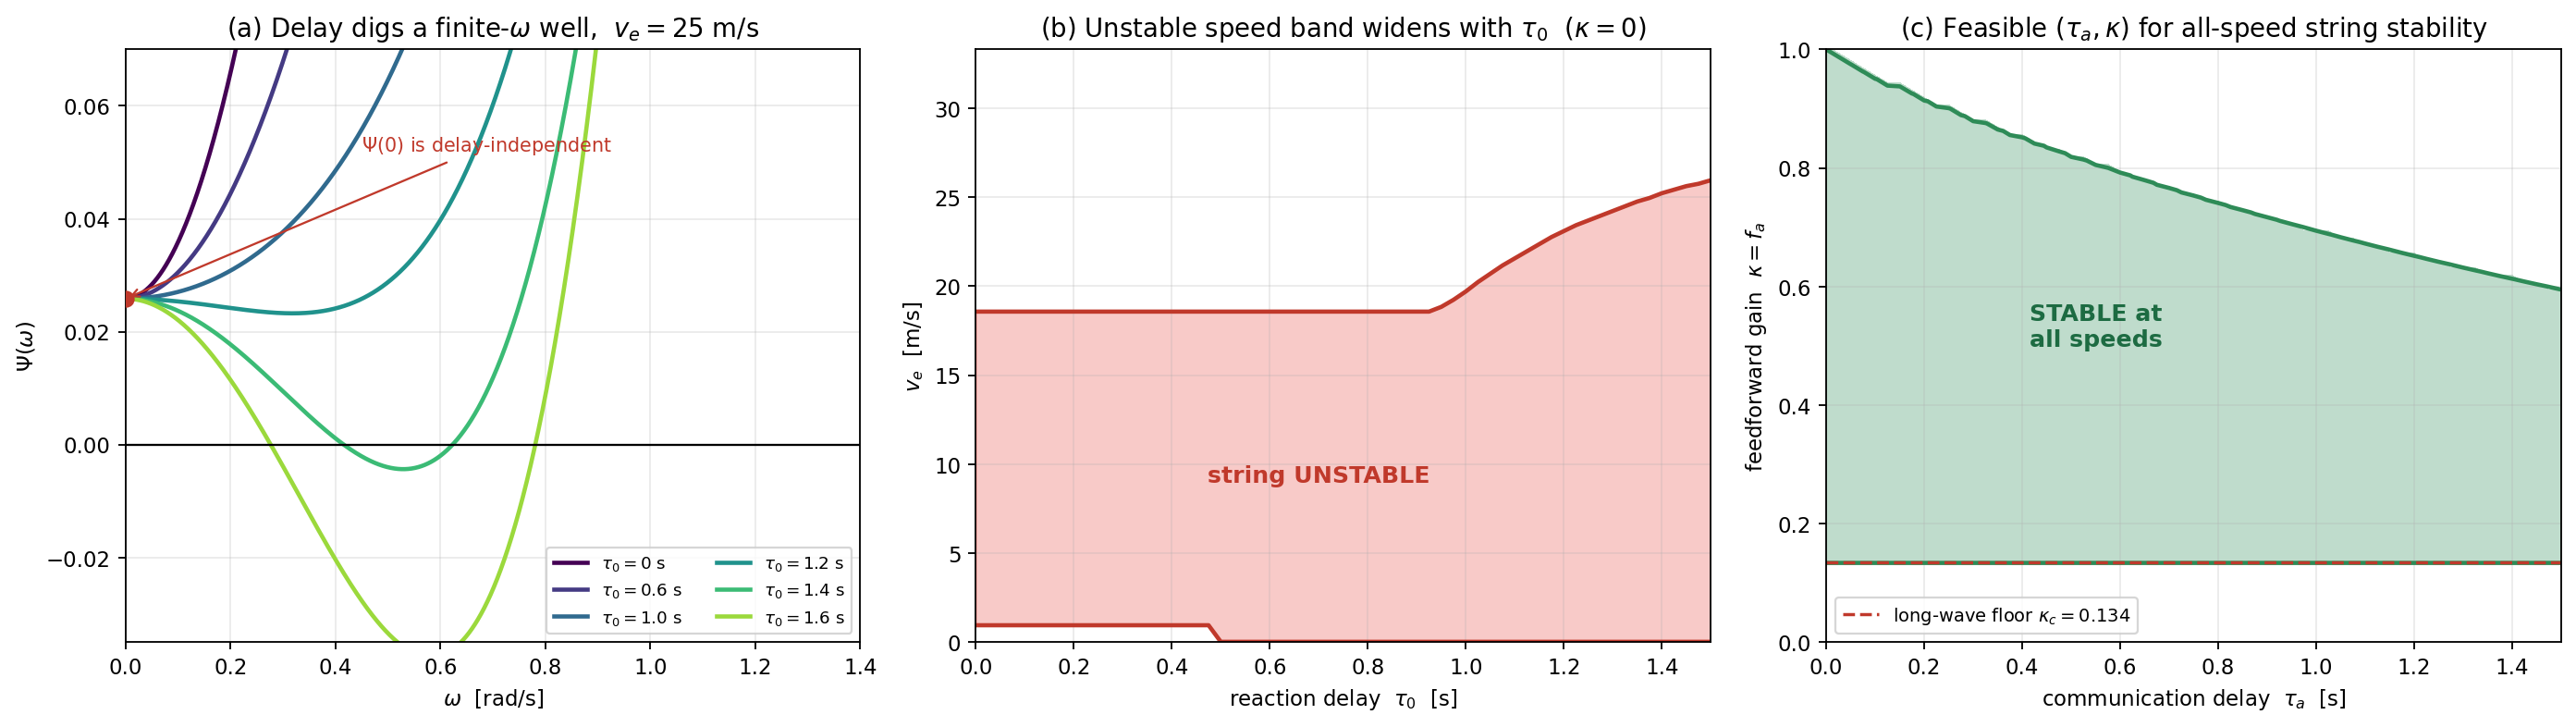
\includegraphics[width=\textwidth]{fig4.png}
\caption{Impact of reaction and communication delays on stability.}
\label{fig:delay-map}
\figurenote{How reaction and communication delays erode stability from the finite-frequency regime. The left plot compares frequency-domain margins for different reaction delays at $v_e=25$ m/s: all curves share the same starting point at $\omega=0$, confirming the delay factor equals 1 at zero frequency; however, as delay increases, the trough at finite frequencies deepens and crosses the zero line, creating a new instability branch invisible to long-wave analysis. The middle plot projects the worst-case frequency results for each delay onto the speed axis; it shows the low-speed stable region being consumed first, followed by the expansion of the entire unstable band. The right plot shows the feasible region for communication delay versus feedforward gain: the lower stability bound remains largely unchanged, while the upper bound for high gain steadily decreases, illustrating how delay transforms initially beneficial strong feedback into a risk of phase lag. These three plots demonstrate that "delay does not affect the long-wave threshold" is not equivalent to "delay does not affect stability"; any design involving delay requires checking the entire frequency range.}
\end{figure}

\section{Bidirectional coupling and delay}
\sectionstudy{theory}{Bidirectional coupling and delay}{ororsz2004,ororsz2010}



At $f_b\ne0$, the scalar vehicle-to-vehicle transfer function is no longer applicable (

$\iff \left|f_a\right|<\tfrac12 \iff \sigma<1$), and the presence of quasipolynomials renders the finite-dimensional Bilharz closed-form solution inapplicable. In this case, one can:


\begin{itemize}[leftmargin=1.4em,itemsep=3pt]
\item

Retain the closed-form solution for the long-wave condition, which remains independent of delay: $\tfrac12(f_v^2-f_{v_l}^2)\ge(1-f_a-f_b)f_s$;


\item

Handle the finite-wavelength component

\textbf{numerically.}: For each $k$, either scan the neutral stability boundary on $\lambda=i\omega$ using the D-subdivision method, or determine the rightmost eigenvalue by discretizing the time-delay operator via the pseudospectral collocation method.


\end{itemize}

\begin{tcolorbox}[notebox,title=\textbf{Engineering Conclusions}]
\begin{itemize}[leftmargin=1.2em,itemsep=3pt]
\item \textbf{Time delay does not alter the long-wave threshold.}

The "baseline" requirement—whether to include feedforward and, if so, how much—is determined entirely by static partial derivatives; one need not worry about time delay during calibration.


\item \textbf{The penalty for time delay manifests as a limit on the maximum allowable gain.}

For every increase of approximately 0.5 s in communication delay, the upper bound of the usable $\kappa$ in this example drops by approximately $0.1$–$0.2$. A combination of high gain ($+$) and long delay is dangerous.


\item \textbf{Reaction delay is generally more detrimental than communication delay.}

$\tau_0$ acts simultaneously on the three terms involving $f_s,f_v,f_{v_l}$ and contributes a consistently negative first-order term, $2f_v\tau_0$, to $\Lambda$; communication delay affects only the feedforward term, appearing in the form of $(\tau_a-\tau_0)$. When the two delays are similar, certain phase effects may cancel each other out.


\item

This leads to a counterintuitive design tip:

\textbf{Artificially delay the feedforward signal to synchronize it with the perception delay.}($\tau_a\approx\tau_0$) is actually more stable than the "as fast as possible" case, because the $-2f_af_{v_l}(\tau_a-\tau_0)$ term in $\Lambda$ is positive at $\tau_a<\tau_0$ and negative at $\tau_a>\tau_0$.


\end{itemize}
\end{tcolorbox}

\section{Numerical verification E8: Long-wave threshold remains unchanged; finite-frequency potential well deepens.}
\sectionstudy{experiment}{Numerical verification E8: Long-wave threshold remains unchanged; finite-frequency potential well deepens.}{ororsz2004,ororsz2010}



The experiment consists of two stages. The first stage calculates only $\Psi(0)$ to check whether the long-wave threshold remains constant across different delays; the second stage performs a fine sweep of $\Psi(\omega)$ at $\omega\in[0,6]$ rad/s, using $\min_\omega\Psi=0$ to locate finite-frequency instability. Finally, time-domain simulation with a history buffer is used to cross-check the stability sign.



\begin{center}
\small
\captionof{table}{Invariants and finite-frequency results from the E8 delay sweep.}
\label{tab:e8-delay-validation}
\begin{tabular}{p{3.2cm}p{3.4cm}p{3.7cm}p{3.2cm}}
\toprule
\textbf{Sweep} & \textbf{Invariant} & \textbf{Finite-frequency results} & \textbf{Explanation} \\
\midrule
$\tau_0:0\to0.5$ s &

Upper boundary $18.59$ m/s remains unchanged

&

Lower boundary drops from $0.93$ to $0$&The low-speed stability region is the first to be consumed.
\\[3pt]
$\tau_0=1.5$ s &

The long-wave formula still does not include $\tau_0$.

&

The instability zone expands to the range of $0$–$25.98$ m/s.

&

The potential well continues to deepen and widen.
\\[3pt]
$\tau_a:0\to1.5$ s &

The lower bound of $\kappa$ remains constant at $0.134$.

&

The upper bound drops from $1.00$ to $0.60$.

&

Communication delay compresses the gain window.
\\
\bottomrule
\end{tabular}
\end{center}
\tabletext{tab:e8-delay-validation}{

The long-wave threshold remains constant during the sweep of reaction and communication delays, while the results regarding finite-frequency instability vary with the delay. This table demonstrates that "the long-wave condition remains unchanged" is not equivalent to "the stability region of the entire system remains unchanged."
}

\begin{tcolorbox}[resultbox,title=\textbf{Verification of conclusions}]
All $\Psi(\omega)$ curves originate from the same $\Psi(0)$ but dip as delay increases at positive frequencies. Thus, satisfying the "long-wave condition" is merely a necessary condition; even when $\Psi(0)\ge0$ and $\min_{\omega>0}\Psi<0$ hold, finite-wavelength growth still appears in simulations. This experiment directly verifies why delay does not alter the minimum required feedforward amount but does reduce the maximum allowable gain.

\end{tcolorbox}

\section{Specific trajectory results: Reaction delay induces stop-and-go waves.}
\sectionstudy{experiment}{Specific trajectory results: Reaction-delay-induced stop-and-go waves}{ororsz2004,ororsz2010}

Figure ~\ref{fig:traj-s5}: fixed at $v_e=19$ m/s. Without delay, the value is $\sigma_v(1800)/\sigma_v(0)=0.0106$; upon introducing a delay of $\tau_0=1.10$ s, the ratio rises to $165.68$, and the system enters a state of finite-amplitude stop-and-go waves. The probe vehicle speed ranges from $0$ to $26.01$ m/s, and the spacing ranges from $3.04$ to $60.26$ m. The minimum spacing remains positive; thus, the strong oscillations observed in the figure are not numerical artifacts caused by vehicle overlap. This case study demonstrates that even if the high-speed operating point is stable in the absence of delay, the system can be driven into an unstable regime by reaction delay.

\begin{figure}[htbp]
\centering
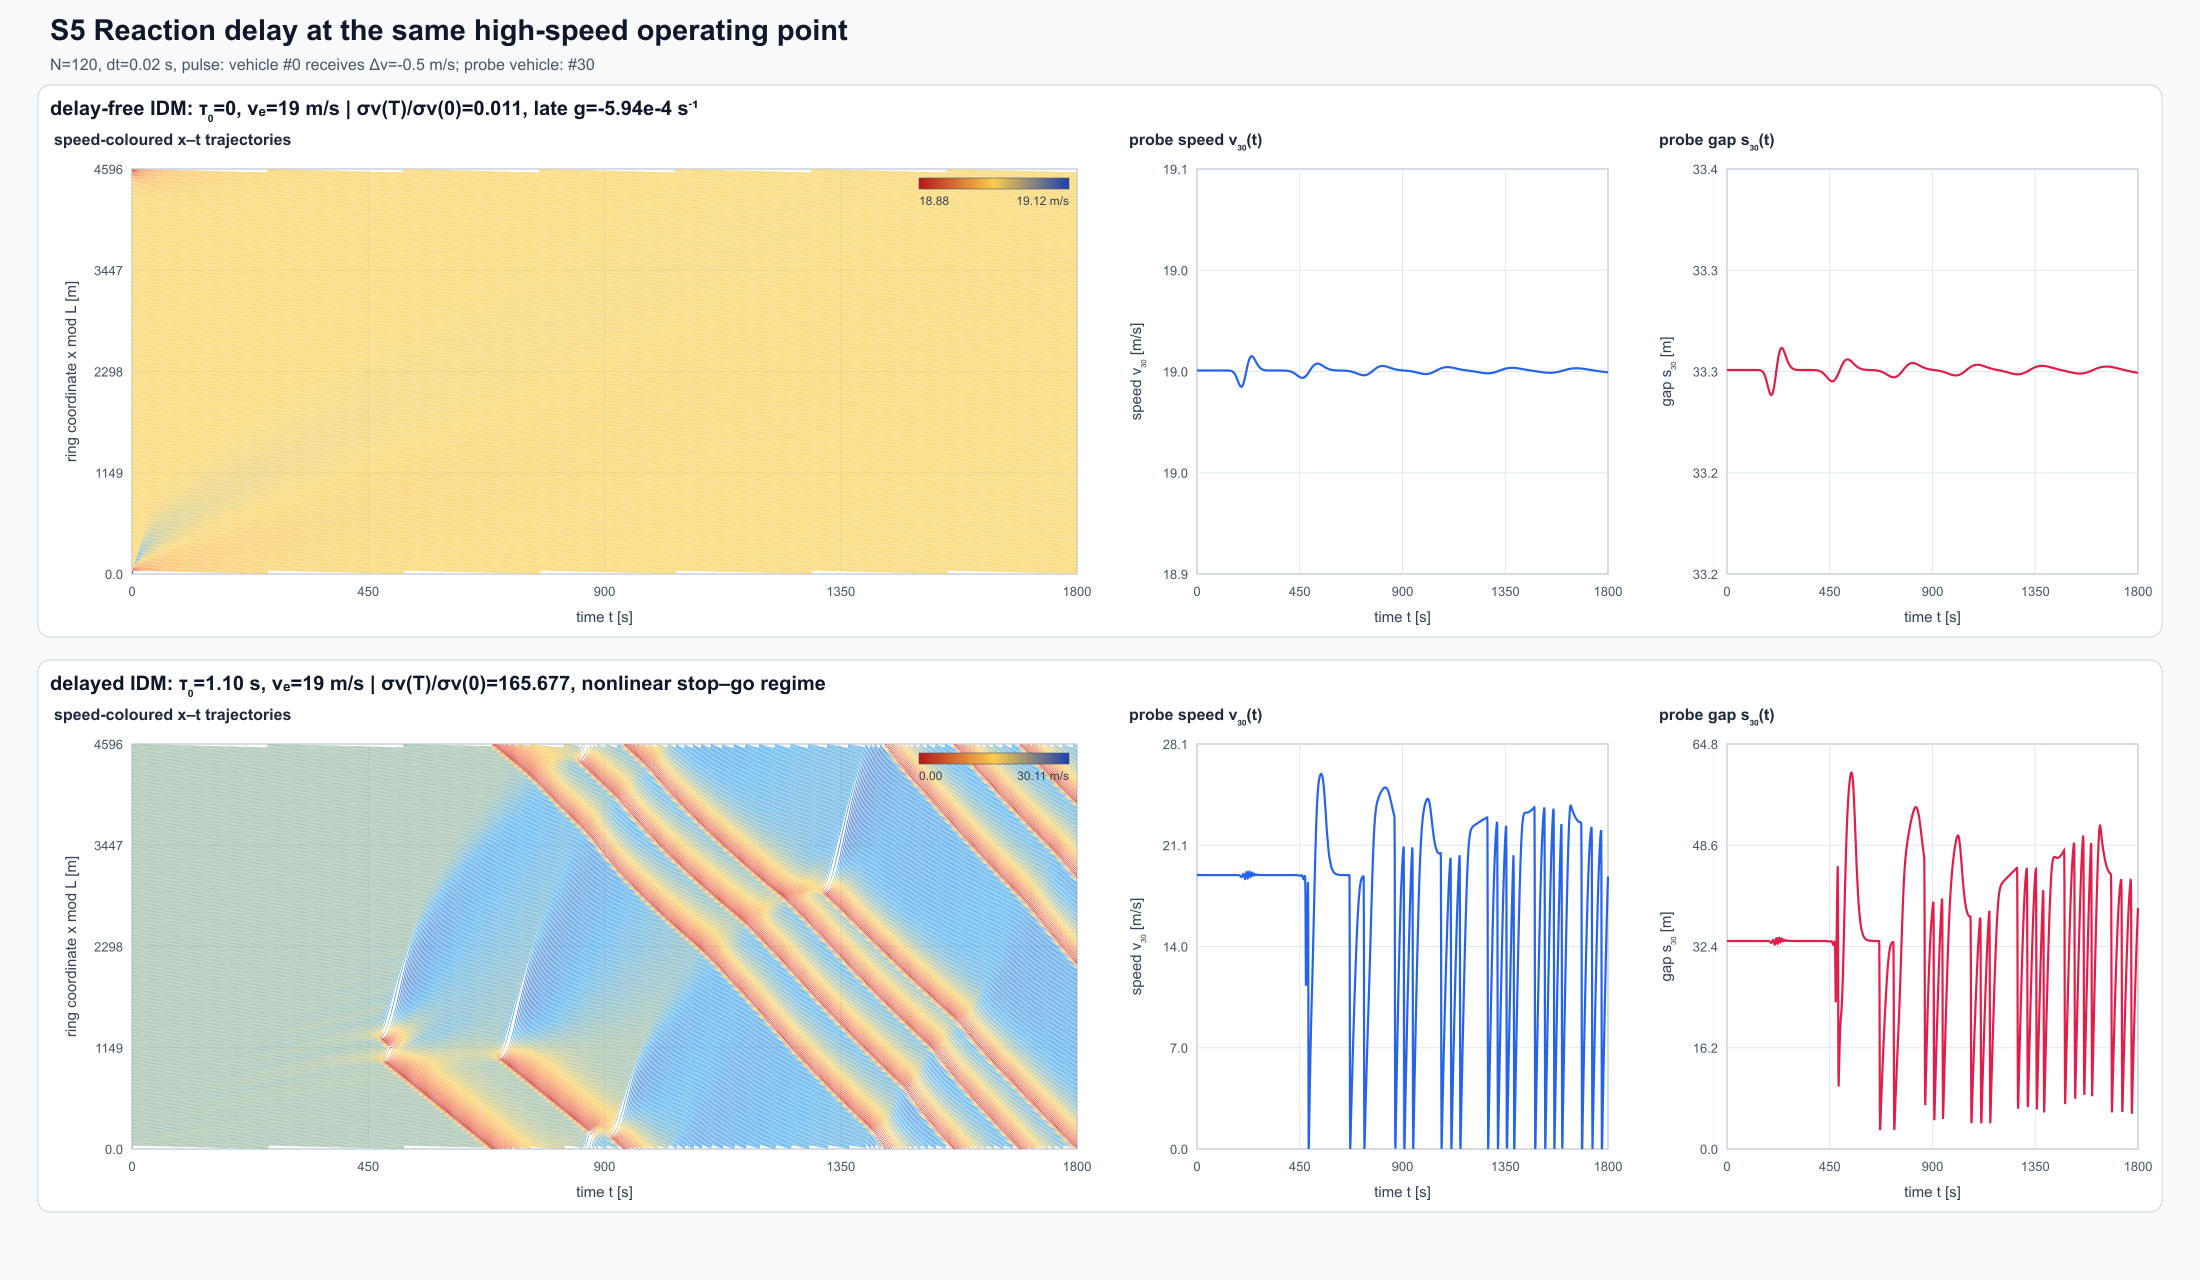
\includegraphics[width=\textwidth]{sim_s5_delay.png}
\caption{S5: Reaction-delay-induced stop-and-go waves.}
\label{fig:traj-s5}
\figurenote{S5 illustrates the transformation of the finite-frequency negative margin shown in Figure ~\ref{fig:delay-map} into actual stop-and-go waves. Both lines utilize a speed of $v_e=19$ m/s—close to the original stability boundary—and differ only in that the reaction delay is changed from zero to 1.10 s; thus, the discrepancy cannot be attributed to density or initial perturbations. For the line without delay, the color bands fade as they propagate upstream, and probe speeds and spacings converge; in contrast, the line with delay exhibits multiple color bands that chase, merge, and intensify, causing the 30th vehicle to repeatedly enter a low-speed state accompanied by significant spacing compression and expansion. The waveform is not the longest single sine wave but rather exhibits shorter spatiotemporal scales selected by the critical finite frequency—a phenomenon that would be overlooked if one considered only $\omega\to0$. This figure demonstrates that a 1.10 s delay can push an analytically stable operating point into a nonlinear stop-and-go wave state, highlighting the necessity of co-designing communication/perception latency with control gains.
}
\end{figure}

%==================================================================
\sectionwrapup{Reaction and communication delays transform the characteristic polynomial into a quasipolynomial, introducing an infinite number of roots. While the static threshold for long waves may remain unchanged, the finite-frequency phase margin shrinks significantly; consequently, it is essential to scan the delay spectrum beyond the target gain and verify the most critical roots using time-domain simulation.}

\PART{VI}{Breaking Homogeneity: Heterogeneous Platoons and Mixed Traffic}

%==================================================================
\chapter{Heterogeneous Platoons: \texorpdfstring{$F_n\ne F_{n-1}$}{Differing vehicle models}}
\label{sec:het}
\chapterguide{Why do different propagation results emerge even when the vehicle mix is identical but the arrangement differs?}{

After the failure of Fourier diagonalization, this chapter shifts to the chain product of vehicle-specific transfer functions, establishing concepts such as weighted prefix sums, sequencing effects, and rules for AV adjacency, while applying the penetration-rate-versus-speed 2D stability domain to mixed traffic design.}The preceding chapters assumed a uniform convoy. In reality, traffic flow varies in vehicle type, driving style, and whether it is equipped with ACC/CACC; each vehicle has its own $F_n$. This chapter provides the corresponding analytical framework.

\section{Equilibrium state is no longer uniform.}
\sectionstudy{model}{Equilibrium state is no longer uniform.}{talebpour2016,feng2019,stern2018}

Balance requires all cars

\textbf{to have the same speed.}

(Otherwise, the spacing will continue to change), but

\textbf{the spacing is different for each car.}

: The density on the basic graph is changed to the average spacing $\bar s_e(v_e)=\frac{1}{N}\sum_n s_e^{(n)}$, i.e., $\rho = 1/\left(\bar s_e + \bar l\right)$.

Each vehicle has its own partial derivative at its equilibrium point. The linearized equation is:

\begin{equation}
\ddot y_n = f_s^{(n)}\left(y_{n-1}-y_n\right) + f_v^{(n)}\dot y_n + f_{v_l}^{(n)}\dot y_{n-1}
\end{equation}

\section{Structural change: Loss of translation invariance}
\sectionstudy{theory}{Structural change: Loss of translation invariance}{talebpour2016,feng2019,stern2018}

\begin{tcolorbox}[notebox,title=\textbf{Fourier mode failure} [] Coefficients change with $n$, matrix $A,B$

\textbf{No longer a cyclic matrix}

, DFT basis no longer diagonalizes them (see comparison)\S\ref{sub:circulant}). Spatial Fourier analysis in heterogeneous vehicle platoons

\textbf{is not applicable at all}

.

However,

\textbf{the unidirectional cascade structure still}

: $y_n$ depends only on $y_{n-1}$. Therefore, the transfer function method

\textbf{is actually the only effective tool here}

—exactly the opposite of the bidirectional coupling case.


\end{tcolorbox}

\section{Vehicle-to-vehicle transfer functions and chain products}
\sectionstudy{theory}{Vehicle-to-vehicle transfer functions and chain products}{swaroop1996,ploeg2014,feng2019}



Apply the Laplace transform individually to the $n$-th vehicle:


\begin{tcolorbox}[keybox]
\begin{equation}
G_n(\lambda) = \frac{\hat y_n}{\hat y_{n-1}}
= \frac{f_s^{(n)} + f_{v_l}^{(n)}\lambda + f_a^{(n)}\lambda^2}{\lambda^2 - f_v^{(n)}\lambda + f_s^{(n)}}
\end{equation}
($f_a^{(n)}$ is the feedforward gain for the acceleration of the preceding vehicle; set to $0$ when there is no feedforward.) The gain of the disturbance transmission from the $0$-th vehicle to the $j$-th vehicle is

\textbf{the product}：
\begin{equation}
\frac{\hat y_j}{\hat y_0} = \prod_{n=1}^{j} G_n(\lambda)
\end{equation}
\end{tcolorbox}

\section{Three-level criterion}
\sectionstudy{theory}{Three-level criterion}{talebpour2016,feng2019,stern2018}

\begin{table}[htbp]
\centering
\small
\caption{Three-level stability criterion for heterogeneous unidirectional platoons.}
\label{tab:heter-three-levels}
\begin{tabular}{p{2.6cm}p{5.4cm}p{5.8cm}}
\toprule
& \textbf{Condition} & \textbf{Meaning} \\
\midrule


(i) Local stability

&

$f_s^{(n)}>0$, $f_v^{(n)}<0$; vehicle-by-vehicle

&

Each vehicle does not diverge on its own
\\[4pt]
(ii) \textbf{Strict}

String stability

&

$\left\|G_n\right\|_\infty\le1$; vehicle-by-vehicle

&

Strongest; independent of platoon composition and ordering

\textbf{Completely independent}

, safe under any mixing
\\[10pt]
(iii) \textbf{Platoon}

String stability

& $\max\limits_\omega\left|\prod_{n\le j}G_n(i\omega)\right|\le1$，$\forall j$ &

Allows individual vehicles to amplify disturbances, provided they are offset by attenuating vehicles ahead or behind;

\textbf{Depends on ordering} \\
\bottomrule
\end{tabular}
\end{table}



Table \ref{tab:heter-three-levels} presents three levels, ranging from "individual vehicle non-divergence" to "no amplification for any prefix." Condition (ii) is the strongest but also the most conservative; in actual traffic, almost no human-driven vehicle can satisfy it. In engineering practice, Condition (iii) is typically used; it allows local amplification to be offset by subsequent stable vehicles but requires the preservation of ordering information. \section{Feedback Loops: The closed-loop equation, the frequency-domain sufficiency condition, and pre-amplification are not the same thing.}
\sectionstudy{model}{Feedback Loops: The closed-loop equation, the frequency-domain sufficiency condition, and pre-amplification are not the same thing.}{talebpour2016,feng2019,stern2018}

\subsection{The closure equation is not an identity that holds for arbitrary $\lambda$}



Let the open-loop transfer function for a full circuit be denoted as
\[
H(\lambda):=\prod_{n=1}^{N}G_n(\lambda).
\]





Starting from the reference vehicle $0$, the signal is passed from vehicle to vehicle for one lap, resulting in $\hat y_N=H(\lambda)\hat y_0$; the loop closure also requires $\hat y_N=\hat y_0$. For non-zero modes, $\hat y_0\ne0$, we therefore obtain







\begin{tcolorbox}[keybox,title=\textbf{Circuit Characteristic Equation}]
\begin{equation}
\prod_{n=1}^{N} G_n(\lambda) = 1.
\label{eq:heter-ring-closure}
\end{equation}
\end{tcolorbox}







The meaning of Equation ~\eqref{eq:heter-ring-closure} is “\textbf{Find which specific $\lambda$ values make the product equal to 1}




,” rather than stating that the product is always equal to 1 for any $\lambda$. This is exactly the same as $\det(\lambda I-A)=0$, which involves solving an eigenvalue equation rather than an identity. In the uniform case, it degenerates into $G(\lambda)^N=1$, whose $N$ possible phases are

\[
G(\lambda)=\exp\!\left(i\frac{2\pi m}{N}\right)=e^{ik_m},
\qquad k_m=\frac{2\pi m}{N},\quad m=0,\ldots,N-1,
\]

which is precisely the discrete wavenumber from Chapter ~\ref{sec:appx}~. When $\lambda=0$, all vehicles undergo an equal translation, with both spacing and speed remaining constant; this is a neutral mode resulting from translational symmetry and should be excluded separately when assessing the stability of traffic disturbances.










\subsection{Why is it necessary to check $|H(i\omega)|$ in addition to the closed-form equations?}










To accurately determine the stability of a loop, one must find all roots of the equation ~\eqref{eq:heter-ring-closure} and verify whether all roots, except for the translation roots, satisfy $\operatorname{Re}\lambda<0$. To avoid directly solving complex transcendental equations, a more easily computable sufficient condition can be used at the boundary of the stable region, $\lambda=i\omega$:










\begin{tcolorbox}[keybox,title=\textbf{Sufficient Condition for the Modulus of the Loop}]
\begin{equation}
\left|H(i\omega)\right|
=\prod_{n=1}^{N}\left|G_n(i\omega)\right| \le 1
\quad \forall\omega
\qquad\Longrightarrow\qquad \text{the ring has no growing modes}.
\label{eq:heter-ring-gain}
\end{equation}
\end{tcolorbox}










The two equations are not contradictory. $H(\lambda)=1$ holds only when




\textbf{the eigenvalue}The condition holds; the expression ~\eqref{eq:heter-ring-gain} treats $\lambda=i\omega$ as a continuous probe point to check the open-loop gain along the entire imaginary axis. For the complex number to be exactly equal to 1, the following must be satisfied simultaneously:

\[
|H(i\omega)|=1,
\qquad
\arg H(i\omega)=2\pi q.
\]

If $|H(i\omega)|<1$, it obviously cannot be equal to 1. Assuming that each vehicle is locally stable—and thus $H$ is analytically definable in the right-half-plane and bounded at high frequencies—the maximum-modulus principle extends the region where the value is strictly less than 1 on the imaginary axis to the open right-half-plane; therefore, no roots of $H(\lambda)=1$ can exist there.




The term “$\le1$” here allows for the neutral case. Due to $G_n(0)=1$, $H(0)=1$ always holds; this corresponds to the aforementioned global translation. To ensure strict asymptotic stability of velocity and separation, the more precise requirement is

\[
|H(i\omega)|<1\quad \forall\omega>0,
\]

or, when the equality holds, to additionally verify that the phase is not $2\pi q$. Conversely, the occurrence of $|H(i\omega)|>1$ at any point does not automatically imply instability: for example, the absolute value of $H(i\omega)=1.2i$ is greater than 1, yet it is not equal to 1. Therefore, the expression ~\eqref{eq:heter-ring-gain} is




\textbf{sufficient but possibly conservative}Amplitude screening; the precise conclusion for a finite $N$ is still determined by the root of equation ~\eqref{eq:heter-ring-closure} or the full Nyquist angle. Numerically (14 sets of random heterogeneous ring paths), 11 sets of amplitude criteria agreed with the direct root calculation, while the other 3 sets showed “the product slightly exceeds 1, but the phase is not closed, and the finite loop remains stable.”










\subsection{What exactly can $j=N$ be used to determine?}

\begin{table}[htbp]
\centering
\small
\caption{Loop stability and the subject of the prefix-free amplification check.}
\label{tab:ring-versus-prefix}
\begin{tabular}{p{3.5cm}p{5.0cm}p{5.2cm}}
\toprule
\textbf{Problem} & \textbf{Subjects to be checked} & \textbf{Conclusion} \\
\midrule







Loop is asymptotically modal stable




&




Roots of $H(\lambda)=\prod_{n=1}^{N}G_n(\lambda)=1$




&




Complete closure involves only $j=N$




\\[4pt]
Sufficient condition based on loop magnitude

&

$|H(i\omega)|\le1$, for all frequencies

&

Still involves only $j=N$, but may be conservative
\\[4pt]
No amplification from a given disturbance source to any intermediate vehicle

&

$H_j(i\omega)=\prod_{n=1}^{j}G_n(i\omega)$, for all $j$ and $\omega$

&

Each prefix must be checked; a stronger condition than loop stability
\\
\bottomrule
\end{tabular}
\end{table}



Table~\ref{tab:ring-versus-prefix} lists three easily confused problems and the quantities to be checked for them. Regarding

\textbf{loop eigenvalues}...is sufficient; however, if safety, comfort, or whether a bounded perturbation was amplified before completing a full circuit are concerns, one cannot look solely at the terminal point. A loop lacks a natural "head of the line": if a perturbation can originate from any vehicle, the condition of no internal amplification requires checking the cyclic prefix for every possible starting point. Since the scalar product is commutative, the order of vehicles—once their individual $G_n$ values are fixed—does not alter the loop's characteristic equation; the set of prefixes, however, changes depending on the perturbation's origin and the vehicle arrangement.



\section{Long-wave criterion: Weighted prefix sum}
\sectionstudy{theory}{Long-wave criterion: Weighted prefix sum}{talebpour2016,feng2019,stern2018}



Expand each vehicle for small $\omega$ (using results from Chapter \ref{sec:lead}):
\begin{equation}
\left|G_n(i\omega)\right|^2 \approx 1 - \eta_n\,\omega^2,
\qquad
\boxed{\ \eta_n = \frac{\left(f_v^{(n)}\right)^2-\left(f_{v_l}^{(n)}\right)^2-2f_s^{(n)}\left(1-f_a^{(n)}\right)}{\left(f_s^{(n)}\right)^2}\ }
\end{equation}
The logarithmic approximation here can be derived step-by-step. Given that $\ln|G_n|=\tfrac12\ln|G_n|^2$ and $\ln(1+x)=x+O(x^2)$, it follows that
\[
\ln|G_n(i\omega)|
=\frac12\ln\!\left[1-\eta_n\omega^2+O(\omega^4)\right]
=-\frac12\eta_n\omega^2+O(\omega^4).
\]

The factor $1/2$ comes from the square of the mode length, and the negative sign comes from $\ln(1-x)\approx-x$. Thus, the product of the first $j$ vehicles becomes a sum:

\[
\ln\left|\prod_{n=1}^{j}G_n(i\omega)\right|
\approx-\frac{\omega^2}{2}\sum_{n=1}^{j}\eta_n.
\]










\begin{tcolorbox}[keybox,title=\textbf{Long-wave prefix conditions for an open fleet starting from a given perturbation source}]
\begin{equation}
\sum_{n=1}^{j}\eta_n \;\ge\; 0
\qquad \forall\, j = 1,\dots,N
\label{eq:heter-prefix}
\end{equation}
\end{tcolorbox}










Three points are worth noting:





\begin{itemize}[leftmargin=1.4em,itemsep=4pt]
\item $\eta_n$ is




\textbf{Single-vehicle long-wave stability index}




: $\eta_n>0$ attenuates disturbances for this vehicle, while $\eta_n<0$ amplifies them. For a homogeneous fleet, the condition reverts to $\eta\ge0$, which is the original criterion.







\item \textbf{The weight is $1/f_s^2$.}




$f_s$: Small vehicles (with sluggish spacing responses, such as heavily loaded trucks) carry a very high weight in the summation—a single “sluggish” vehicle can offset the performance of several good vehicles.







\item




The condition is




\textbf{a prefix sum}




rather than a total sum: once the value drops below zero at any point along the way, the disturbance has already been amplified into the nonlinear region, and it is too late to correct it afterward.







\end{itemize}










The condition in equation ~\eqref{eq:heter-prefix} must be separated from the $j=N$ condition for the circuit. Taking only $j=N$ yields

\[
S_N:=\sum_{n=1}^{N}\eta_n\ge0,
\]

which merely indicates that the entire formation has a non-negative




\textbf{total long-wave budget}...and is also an essential component of the low-frequency conditions for a full lap on the circuit; it does not guarantee that the disturbance will not be amplified at any intermediate position. It is entirely possible for a $S_N>0$ to occur, but for a specific $S_j<0$: the disturbance is first amplified by an unstable vehicle and then suppressed by a stable vehicle. To ensure no amplification within an open fleet, all $j$s must be checked; for the ring track’s asymptotic eigenvalues, complete closure requires only $j=N$; if it is also required that no local amplification occurs on the ring track starting from any perturbation origin, then the prefixes at all cycle cutpoints must be rechecked.










\section{Numerical Example: Mixed Autonomous Vehicle Fleet}
\sectionstudy{experiment}{Numerical Example: Mixed Autonomous Vehicle Fleet}{talebpour2016,feng2019,stern2018}










Assume that the two vehicle types share the IDM parameters from Chapter ~\ref{sec:num}~, with the only difference being that AVs use lead-vehicle acceleration feedforward $\kappa=0.5$:

\begin{equation}
\eta_{\rm AV} = \eta_{\rm HV} + \frac{2\kappa}{f_s}
\end{equation}




Let the AV penetration rate be $p$. For now, we will only consider $j=N$, i.e., use

\[
\frac{S_N}{N}=p\,\eta_{\rm AV}+(1-p)\eta_{\rm HV}\ge0
\]

to calculate “whether the convoy configuration has sufficient total stability budget,” yielding










\begin{tcolorbox}[keybox,title=\textbf{Minimum penetration rate required for the formation/circuit long-wave total budget}]
\begin{equation}
p_{\min} = \frac{-\eta_{\rm HV}}{\eta_{\rm AV}-\eta_{\rm HV}}
= \frac{2f_s + f_{v_l}^2 - f_v^2}{2\kappa\,f_s}
\end{equation}
\end{tcolorbox}










This $p_{\min}$ is




\textbf{Total threshold}: It is meaningful for determining the ratio of the two vehicle types and the budget for a full lap of the circuit, but it is not a sufficient condition for the formula ~\eqref{eq:heter-prefix} under arbitrary permutations. Even after specifying the ratios, all $S_j$ values generated by the arrangement must still be checked; if safety is required for any arrangement, one must revert to the strict per-vehicle condition $\|G_n\|_\infty\le1$, which the HDV in this example does not satisfy.




For the parameters in this example, $p_{\min}$ varies with speed, peaking at $v_e\approx9$ m/s:










\begin{table}[htbp]
\centering
\caption{Long-wave indices and minimum total AV at different equilibrium speeds.}
\label{tab:heter-pmin-speed}
\begin{tabular}{rccccc}
\toprule
$v_e$ [m/s] & 3 & 6 & 9 & 12 & 16 \\
\midrule
$\eta_{\rm HV}$ & $-0.574$ & $-1.378$ & $-2.088$ & $-2.532$ & $-2.010$ \\
$\eta_{\rm AV}$ & $+2.676$ & $+4.130$ & $+5.724$ & $+7.727$ & $+12.10$ \\
$p_{\min}$ & 17.7\% & 25.0\% & \textbf{26.7\%} & 24.7\% & 14.2\% \\
\bottomrule
\end{tabular}
\end{table}










Table ~\ref{tab:heter-pmin-speed} presents the long-wave indices for HDV and AV at five representative speeds, and calculates the minimum penetration rate based on the total budget constraints. The most unfavorable point occurs at $v_e\approx9$ m/s; therefore,




\textbf{The minimum penetration rate required for the total budget across the entire speed range for formation flying and circuit operations is $26.7\%$.}




 This value is inversely proportional to $\kappa$: raising the feedforward gain to $\kappa=1$ requires only about $13\%$, while lowering it to $\kappa=0.25$ requires more than half that amount. It answers the question of “whether the total amount is sufficient”; the prefix curve in the next section answers whether “these stabilization capabilities appear in the propagation path in a timely manner.”










\section{Ordering Effect}
\sectionstudy{theory}{Ordering Effect}{talebpour2016,feng2019,stern2018}
\label{sub:hetorder}

\begin{figure}[htbp]
\centering
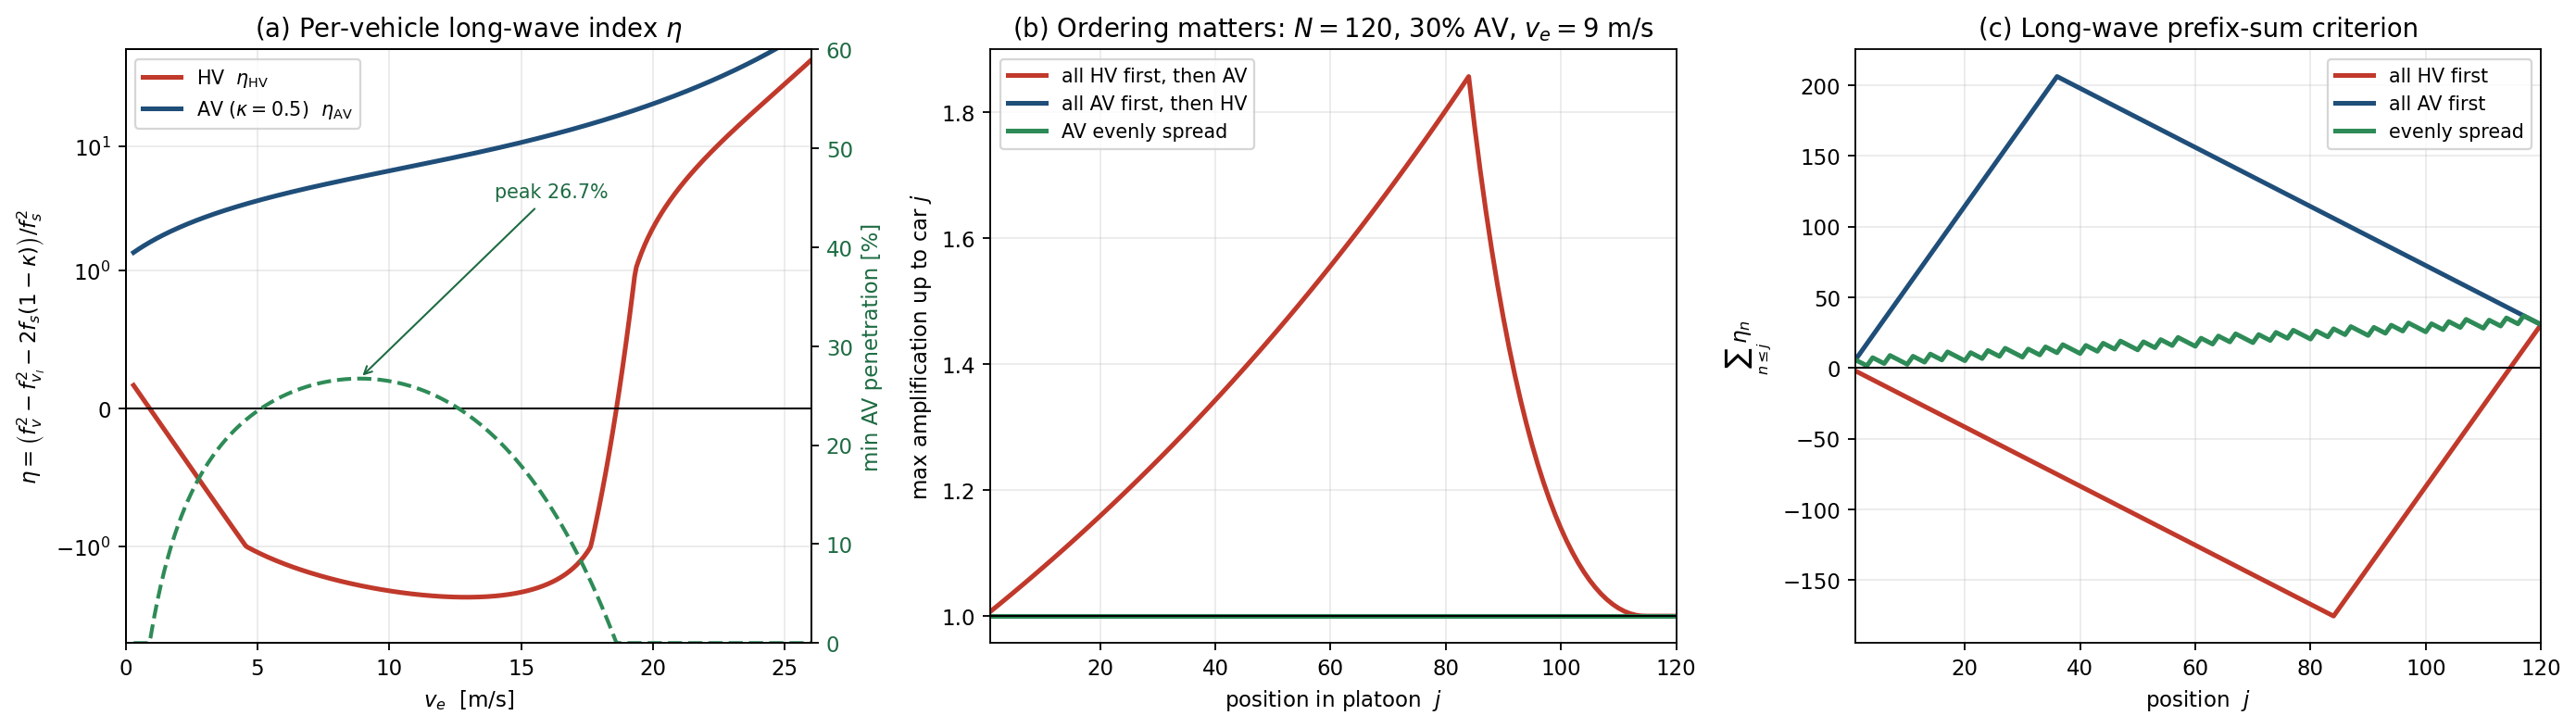
\includegraphics[width=\textwidth]{fig8.png}
\caption{Total Budget and Ordering Effects in Heterogeneous Fleets.}
\label{fig:heter-order-budget}
\figurenote{What do “Overall Formula” and “Vehicle Ordering” control in a heterogeneous fleet? The left figure calculates the long-wave indices for HDVs and AVs based on the equilibrium speed and determines the minimum AV penetration rate using a weighted sum; The curve reaches its most unfavorable peak of 26.7 at approximately $v_e=9$ m/s \% , indicating that the penetration rate threshold must cover the entire speed operating range and cannot be determined based solely on a single convenient operating condition. The middle figure fixes $N=120$ and 30 \% AV, and compares the cumulative amplification per vehicle for the three sorting orders: all three curves return to 1 at the end, verifying that the full-lap product is independent of the arrangement when the scalar $G_n$ is fixed; however, when 84 HDVs are placed in the front section of the propagation path, the mid-lap peak reaches 1.857. The long-wave prefix in the figure on the right explains the origin of this peak: the negative contribution from unstable HDVs accumulates first, until the positive contribution from subsequent AVs pulls the total back to a non-negative value. This figure demonstrates that a ring track only requires the final total budget to be non-negative, whereas an open fleet—if it wants to ensure that amplification does not occur for any intermediate vehicles—must check all prefixes; “end-state stability” cannot substitute for “in-process safety.”}
\end{figure}





The “front of the line” shown in the figure is not the lead vehicle naturally present on the loop, but rather the first position along the direction of disturbance propagation after the loop is split at the disturbance injection point. In this scenario, there are 84 HDVs and 36 AVs, and

\[
\eta_{\rm HDV}=-2.088,
\qquad
\eta_{\rm AV}=5.724,
\qquad
S_{120}=84(-2.088)+36(5.724)=30.672>0.
\]

therefore, the total budget for a full lap is the same for all three arrangements. If all HVs are at the front, then

\[
S_{84}=84(-2.088)=-175.392,
\qquad
S_{84+r}=-175.392+5.724r.
\]

the prefix sum does not turn positive until the 31st AV appears, i.e., $j=115$; therefore, this arrangement violates equation ~\eqref{eq:heter-prefix} at $j=1,\ldots,114$. If all AVs are at the front, a positive budget of $S_{36}=206.064$ is first accumulated; although the subsequent 84 HDVs continue to deplete it, $S_j\ge0$ is maintained until the end. The uniform arrangement achieves the same result by shortening the continuous HV segment.




“Ending with $1.0000$” cannot be interpreted to mean that all frequencies pass through unchanged. The vertical axis in the figure represents $\max_{\omega\ge0}|H_j(i\omega)|$; because of $G_n(0)=1$, any stable prefix has a gain of 1 at $\omega=0$, while non-zero frequencies have a gain less than 1, so the maximum value is displayed as 1.0000. The red curve exceeds 1 at a finite number of non-zero frequencies, resulting in a peak of 1.857.










\begin{tcolorbox}[keybox,title=\textbf{Key Conclusions}]
\begin{equation}
\prod_{n=1}^{N}\left|G_n\right| \ \text{independent of ordering (products commute)},
\qquad
\max_j\left|\prod_{n\le j}G_n\right| \ \text{strongly depends on ordering}
\end{equation}
\begin{itemize}[leftmargin=1.2em,itemsep=3pt]
\item \textbf{The lap is asymptotically stable: check $j=N$.}




After fixing $G_n$ for each car, the complete product is commutative; therefore, the characteristic equation and the total gain for a full lap depend only on the formula and not on the arrangement.


\item \textbf{Open Fleet / No Internal Amplification: Check all $j$s.}




 In this example, all three arrangements end with $1.0000$, but when the HV is concentrated in the early part of the propagation path, it amplifies midway to $1.857$; therefore, it does not satisfy the equation ~\eqref{eq:heter-prefix}, even though the loop eventually decays.







\item \textbf{$26.7\%$ only addresses the total quantity; it does not address the order.}




It guarantees $S_N\ge0$; under this premise, the AV must still be placed at the front end of the disturbance path or distributed as evenly as possible to prevent $S_j$ from falling below zero midway.







\end{itemize}
\end{tcolorbox}

\section{AV acceleration feedback: Feedforward capability depends on the type of the leading vehicle}
\sectionstudy{model}{AV acceleration feedback: Feedforward capability depends on the type of the leading vehicle}{talebpour2016,feng2019,stern2018}







\label{sub:mixed}




The above treats $f_a^{(n)}$ as an attribute of the vehicle itself. However, in mixed traffic, this assumption is overly optimistic:




\textbf{Feedforward requires the leading vehicle to provide acceleration information}




, and the quality of that information depends on




\textbf{the type of vehicle ahead}。

\begin{table}[htbp]
\centering
\small
\caption{the actual feedforward gain for adjacent AV/HDV combinations.}
\label{tab:pair-dependent-gain}
\begin{tabular}{p{4.4cm}p{4.4cm}p{4.6cm}}
\toprule







The $n$th vehicle is& The $n-1$ vehicle is




&




 Effective gain $f_a^{(n)}$



\\
\midrule
HV &




 Arbitrary




& $0$ \\
AV &




 AV (V2V broadcastable)




&




 $\kappa$ (complete, low noise, low latency)



\\
AV &




 HV (radar estimate only)




&




 $\kappa_0<\kappa$ (high differential noise, must be conservative)



\\
\bottomrule
\end{tabular}
\end{table}










Table ~\ref{tab:pair-dependent-gain} gives the adjacent pair rules used in this chapter: HDV does not use feedforward, AVs following AVs achieve the full V2V gain $\kappa$, while AVs following HDVs can only use the radar-estimated gain $\kappa_0$. Therefore, the same number of AVs will produce different effective control totals depending on the neighboring structure.










\begin{tcolorbox}[notebox,title=\textbf{This introduces a new structural effect}]

$\eta_n$ now depends on




\textbf{the combination of two adjacent vehicles},




 and not just the vehicle type itself. Thus

\[
\sum_{n}\eta_n = N_H\,\eta_{\rm HV} + \left(N_A-q\right)\eta_{\rm AV}^{(\kappa_0)} + q\,\eta_{\rm AV}^{(\kappa)}
\]

where $q$ is the number of adjacent AV--AV pairs




\textbf{in the fleet}。\textbf{Even the total has become dependent on the sort order}




—This contrasts with





\ref{sub:hetorder}’s assertion that “the total amplification is independent of the sort order,” since that assumes $\eta_n$ is fixed.







\end{tcolorbox}

\subsection{Penetration Rate: The Cost of Dispersed Deployment}










Review $\eta_{\rm AV}^{(\kappa)} = \eta_{\rm HV} + 2\kappa/f_s$. For the IDM parameters in Chapter ~\ref{sec:num}~, consider $\kappa=0.5$ (V2V) and $\kappa_0=0.15$ (radar estimation):










\begin{table}[htbp]
\centering
\caption{Speed-dependent penetration rates required for isolated AVs versus continuous formations.}
\label{tab:dispersed-versus-grouped-pmin}
\begin{tabular}{rccccc}
\toprule
$v_e$ [m/s] & $f_s$ & $\eta_{\rm HV}$ & $\eta_{\rm AV}^{(\kappa_0)}$ & $\eta_{\rm AV}^{(\kappa)}$ &




$p_{\min}$ (Dispersed/Formation)



\\
\midrule
3  & 0.308 & $-0.574$ & $+0.401$ & $+2.676$ & 58.9\% \ / \ 17.7\% \\
6  & 0.182 & $-1.378$ & $+0.274$ & $+4.130$ & 83.4\% \ / \ 25.0\% \\
9  & 0.128 & $-2.088$ & $+0.255$ & $+5.724$ & \textbf{89.1\%} \ / \ \textbf{26.7\%} \\
12 & 0.098 & $-2.532$ & $+0.546$ & $+7.727$ & 82.3\% \ / \ 24.7\% \\
16 & 0.071 & $-2.010$ & $+2.224$ & $+12.10$ & 47.5\% \ / \ 14.2\% \\
\bottomrule
\end{tabular}
\end{table}










Table ~\ref{tab:dispersed-versus-grouped-pmin} presents the long-wave budget for two extreme configurations. When vehicles are dispersed individually, nearly all AVs can only use $\kappa_0$, with the required ratio reaching 89.1 at approximately $v_e=9$ m/s




\%




; when arranged in a continuous formation, most AVs achieve $\kappa$, with the corresponding threshold dropping to 26.7




\%




. This discrepancy illustrates that penetration rates must be reported in conjunction with the communication adjacency structure.










\begin{tcolorbox}[keybox,title=\textbf{Key Figures}]

Minimum penetration rate required for the total budget of long waves across the entire speed range:




\textbf{Dispersed by vehicle: $89.1\%$; continuous formation: $26.7\%$.}




 Even after applying the given ratio and formation, the prefix peak must still be checked.




The discrepancy is more than threefold. The reason is straightforward: an isolated AV is always preceded by an HV and can only receive the downgraded $\kappa_0$; whereas AVs within a formation can communicate with each other via V2V.







\end{tcolorbox}

\subsection{AV Penetration Rate—Speed Two-Dimensional Stability Region}







\label{sub:av-plane}




Reporting only a single “critical AV penetration rate” is still insufficient, because the critical ratio varies significantly with the equilibrium speed. A more comprehensive approach is to use both the AV penetration rate $p_{\rm AV}$ and the equilibrium speed $v_e$ as coordinates, and to recalculate the IDM partial derivatives, AV–AV/AV–HDV adjacency ratios, and full-frequency propagation gains at each operating point, thereby obtaining a two-dimensional stability region

\begin{equation}
\mathcal S_{\rm AV}
=\left\{(p_{\rm AV},v_e):M_{\rm L}(p_{\rm AV},v_e)\ge0,
\ M_{\rm T}(p_{\rm AV},v_e)\ge0\right\}.
\label{eq:av-stability-set}
\end{equation}




For a given configuration, the actual feedforward gain of the $n$th vehicle is not a constant average, but rather

The gain value satisfies $a_n\in\{0,\kappa_0,\kappa\}$.
\label{eq:av-pair-gain}

Here $a_n=0$ for an HDV, $a_n=\kappa_0$ for an AV whose leader is an HDV, and $a_n=\kappa$ for an AV whose leader is another AV.


Therefore, the two-dimensional plot uses two complementary margins. The first is the long-wave margin

\begin{equation}
M_{\rm L}
=\frac1N\sum_{n=1}^{N}
\left[f_v^2-f_{v_l}^2-2f_s(1-a_n)\right],
\label{eq:av-long-margin}
\end{equation}

which determines whether the perturbation grows when $\omega\to0$ is considered. The second is the actual circumferential transfer margin

\begin{align}
G_n(i\omega)
&=\frac{f_s-a_n\omega^2+i\omega f_{v_l}}
{f_s-\omega^2-i\omega f_v},\\
M_{\rm T}
&=\min_{\omega>0}
\left[-\frac1N\sum_{n=1}^{N}\ln|G_n(i\omega)|\right].
\label{eq:av-transfer-margin}
\end{align}

$M_{\rm T}>0$ indicates that the disturbance decays after one full cycle, while $M_{\rm T}<0$ indicates that at least one frequency is amplified after one full cycle. Equation ~\eqref{eq:av-stability-set} requires both conditions to be non-negative to ensure that extremely low-frequency long waves are not overlooked, while also preventing operating conditions characterized by “long-wave stability but limited frequency amplification” from being incorrectly classified as stable.










\begin{figure}[htbp]
\centering
\begin{tabular}{cc}
\textbf{(a) No feedforward: $\kappa=0$} &
\textbf{(b) Mixed traffic: $\kappa=0.45,\ \kappa_0=0.15$}
\end{tabular}
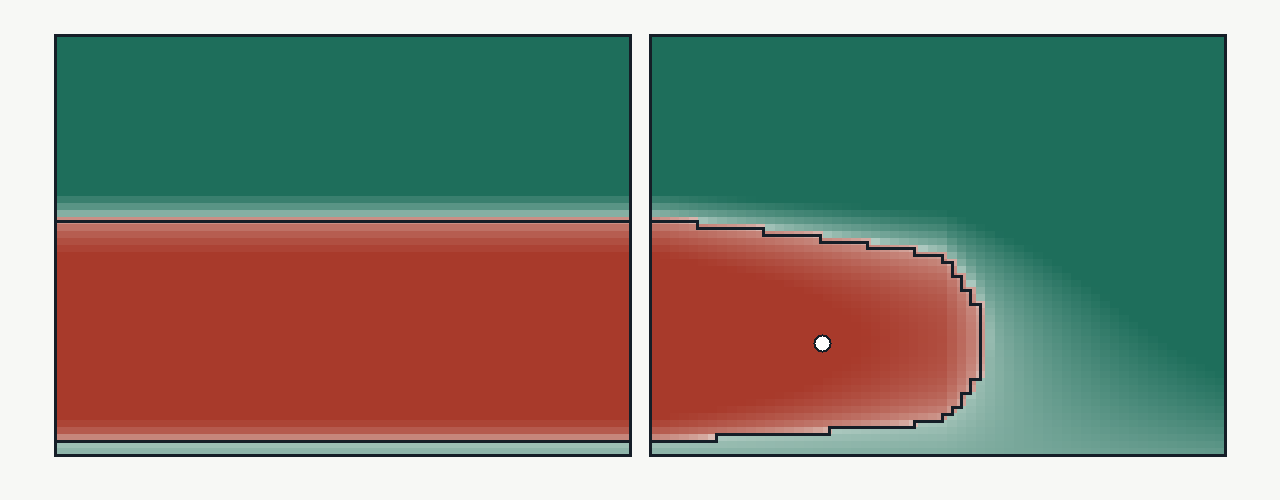
\includegraphics[width=\textwidth]{av_penetration_speed_plane.png}
\vspace{-0.4em}

\small







Horizontal axis: $p_{\rm AV}=0\to100\%$; Vertical axis: $v_e=0\to33.3$ m/s;







\textcolor{teal}{\rule{1.1em}{0.75em}}




Stable,







\textcolor{brick}{\rule{1.1em}{0.75em}}




Instability; the black line represents the boundary, and the white dot represents the current operating point.







\caption{AV permeability–velocity two-dimensional stability region.}
\label{fig:av-stability-plane}
\figurenote{AV Penetration Rate—Two-Dimensional Stability Plane at Equilibrium Speed and Its Causal Comparison. Both figures use $N=60$ and arrange AVs uniformly according to the same rule; the colors indicate stable/unstable regions determined jointly by the long-wave budget and the full-frequency transfer margin. In the left figure, $\kappa=0$ is intentionally set such that, even when the AV proportion on the x-axis changes, vehicle dynamics remain unchanged, and the stability boundary degenerates into the horizontal boundary of the original IDM; this demonstrates that the “AV label” itself does not yield stability benefits. In the right figure, after enabling $\kappa$ and $\kappa_0$, increasing the AV ratio expands the stability region into the originally hazardous low-to-medium speed range; however, the same penetration rate may still result in stability at one speed and instability at another, indicating that the threshold must be a two-dimensional concept within the operating domain. The subtle steps along the boundary correspond to integer jumps in the number of AVs and the adjacent AV–AV pairs when $N=60$ is applied, rather than solution noise. This figure demonstrates that the expansion of the stability region stems from the available feedforward links and their adjacent structures, and provides a direct tool for determining the minimum penetration rate within a given speed range.}
\end{figure}

\begin{tcolorbox}[experimentbox,title=\textbf{Specific readings on a two-dimensional plane}]

Retrieve the parameters for \ref{fig:av-stability-plane}(b). At $p_{\rm AV}=30\%$ and $v_e=8.87$ m/s, the actual average feedforward is only $0.0450$, resulting in

$M_{\rm L}=-0.02300$ and $M_{\rm T}=-0.00233$, so this point remains unstable; the white dot falls within the red zone. When the operating point is shifted to $p_{\rm AV}=73\%$ and $v_e=14.42$ m/s, the average feedforward increases to $0.2500$, resulting in

$M_{\rm L}=+0.02432$ and $M_{\rm T}=+0.00865$, thus becoming stable. This comparison demonstrates that “identical AV ratios” cannot be discussed in isolation from velocity, nor can “identical average gains” substitute for the actual periodic product of adjacent pairs of sequences.







\end{tcolorbox}

\begin{tcolorbox}[notebox,title=\textbf{How to use this figure}]
\begin{enumerate}[leftmargin=1.5em,itemsep=3pt]
\item




First, specify the road’s speed operating range, such as $v_e=5$–$20$ m/s; do not calculate $p_{\min}$ based on a single nominal speed.







\item




Within this speed range, select the rightmost position of the steady-state boundary to obtain the minimum permeability covering the entire operating range; if you are only interested in a specific speed, read the intersection point of that horizontal line with the black boundary.


\item You must redraw after changing $\kappa$, $\kappa_0$, the arrangement, or the number of groups. In particular, under the adjacent pair rule, $p_{\rm AV}$ only determines the number of AVs; the arrangement determines whether these AVs actually receive $\kappa$ or $\kappa_0$.







\item




Positive margins must be left near the boundaries, and verification must be performed using a 1800-second time-domain simulation; the 2D diagram represents the stability region for small perturbations, not the collision safety region, and does not guarantee recovery from arbitrarily large perturbations.







\end{enumerate}
\end{tcolorbox}

\textbf{This directly conflicts with the recommendations in \ref{sub:hetorder}:}




That document states, “Distribute stable vehicles evenly,” while this document states, “They must be grouped.” The real design challenge lies in striking a balance between the two.










\section{Optimal group size: First, clarify what objective “optimal” refers to}
\sectionstudy{theory}{Optimal group size: First, clarify what objective “optimal” refers to}{talebpour2016,feng2019,stern2018}







\label{sec:optimal-grouping}




There is no single answer to the question “How many groups should the AVs be divided into?” that is independent of the objective function. When the number of groups is small, there are more adjacent AV-to-AV pairs within each group, and the full V2V gain $\kappa$ is fully utilized; therefore,




\textbf{the total stability budget for the entire lap is larger}




; when there are more groups, the AVs are more dispersed in road space, and continuous HDV segments are shorter, so \textbf{disturbances are amplified less as they travel toward a stable vehicle}.




These two approaches compete with each other, so we must first distinguish between the following two problems:

\[
\begin{aligned}
\text{Problem A:}&\max_{1\le g\le N_A} S_N(g),\\
\text{Problem B:}&\min_{1\le g\le N_A}H_{\max}(g)
\quad\text{s.t.}\quad S_N(g)\ge S_{\rm res}.
\end{aligned}
\]

Problem A seeks only the total stability margin; its solution necessarily involves combining all AVs into a single group, i.e., $g=1$. Problem B, on the other hand, first specifies the required stability reserve $S_{\rm res}\ge0$ and then seeks to minimize the length of the longest contiguous HDV segment; only under Problem B is the solution “the maximum feasible number of groups that satisfy the stability budget.” The term “optimal grouping” used in this section refers specifically to Problem B described above.




\textbf{Dictionary-Ordered Objective: First ensure the total budget, then improve spatial coverage}




, rather than claiming that more groupings result in a larger total stability margin.










\subsection{Deriving the Upper Bound on the Number of Groups from the Count of Adjacent Pairs}










Suppose $N_A$ AVs are divided into $g=n_{\rm grp}$ non-empty groups. If each group contains $h_r$ AVs, it contributes $h_r-1$ AV–AV adjacent pairs; therefore, regardless of whether the groups are of equal length,

\begin{equation}
q=\sum_{r=1}^{g}(h_r-1)=N_A-g.
\label{eq:group-pair-count}
\end{equation}

The remaining $g$ AVs located at group boundaries follow the HDV and can only use a downgrade gain of $\kappa_0$. The long-wave budget for the entire lap is therefore

\begin{align}
S_N(g)
&=N_H\eta_{\rm HV}+(N_A-g)\eta_{\rm AV}^{(\kappa)}
  +g\eta_{\rm AV}^{(\kappa_0)} \\
&=C-g\,\Delta\eta,
\qquad
C:=N_H\eta_{\rm HV}+N_A\eta_{\rm AV}^{(\kappa)},
\quad
\Delta\eta:=\eta_{\rm AV}^{(\kappa)}-\eta_{\rm AV}^{(\kappa_0)}>0.
\label{eq:group-budget-linear}
\end{align}

Equations ~\eqref{eq:group-budget-linear} show that:\textbf{For every additional group that is cut out, exactly one portion of the total stable budget for $\Delta\eta$ is lost}




. The reason is that the new group will generate an additional AV that is “at the front of the group, with an HDV as the vehicle ahead”: this vehicle was originally part of an AV–AV adjacent pair and could have obtained $\kappa$; after splitting the group, it can only obtain $\kappa_0$, so its contribution to the total decreases from $\eta_{\rm AV}^{(\kappa)}$ to $\eta_{\rm AV}^{(\kappa_0)}$.




First, take the theoretical boundary $S_{\rm res}=0$ without additional reserves. Require $S_N(g)\ge0$, and obtain

\[
g\Delta\eta\le C,
\qquad
g\le\frac{C}{\Delta\eta}.
\]

Substituting $C=N_H\eta_{\rm HV}+N_A\eta_{\rm AV}^{(\kappa)}$ and $\Delta\eta=\eta_{\rm AV}^{(\kappa)}-\eta_{\rm AV}^{(\kappa_0)}$ back into the equation yields







\begin{tcolorbox}[keybox,title=\textbf{Upper Bound on the Number of Groups and Integer Feasible Solutions}]
\begin{align}
g&\le g_{\max}
=\frac{N_A\eta_{\rm AV}^{(\kappa)}+N_H\eta_{\rm HV}}
{\eta_{\rm AV}^{(\kappa)}-\eta_{\rm AV}^{(\kappa_0)}}
=\frac{f_s\left(N_A\eta_{\rm AV}^{(\kappa)}+N_H\eta_{\rm HV}\right)}
{2(\kappa-\kappa_0)}, \\
g^*&=\min\!\left\{N_A,\left\lfloor g_{\max}\right\rfloor\right\},
\qquad S_N(g^*)\ge0.
\label{eq:optimal-group-count}
\end{align}
\end{tcolorbox}


The second equals sign in the formula ~\eqref{eq:optimal-group-count} uses

\[
\eta_{\rm AV}^{(\kappa)}-\eta_{\rm AV}^{(\kappa_0)}
=\frac{2(\kappa-\kappa_0)}{f_s}.
\]

Therefore, $g_{\max}$ can be directly interpreted as “the total stable budget available when all AVs are grouped together” divided by “the stable budget lost for each additional group.” This also implies two feasibility checks: the grouping requires at least $g\ge1$; if $g_{\max}<1$, it means that even if all AVs are combined into a single group, the total budget is still insufficient, and there is no arrangement that satisfies the current constraints. Second, $g$ must be an integer and not exceed $N_A$, so it must be rounded down and compared with $N_A$. In this case, the AV penetration rate, $\kappa$, or $\kappa_0$ should be increased; $g^*=0$ should not be interpreted as a road layout.










\subsection{Why is a large group with the highest total margin not necessarily the most resilient to en route amplification?}





Let’s first consider Problem A. From the equations ~\eqref{eq:group-budget-linear},

\[
S_N(g+1)-S_N(g)=-\Delta\eta<0,
\],

it follows that $S_N(g)$ decreases strictly with $g$. If the sole objective is to maximize the total stability budget for the entire loop, then the conclusion is unambiguous: $g=1$ is optimal. Grouping all AVs into a single cluster preserves the greatest number of AV-AV adjacent pairs and provides the largest attenuation reserve for loop propagation.




The issue is that the total budget only describes the net result after the disturbance has traveled the entire propagation path; it does not limit how much the disturbance is amplified along the way. A large AV group often results in the remaining HDVs forming very long continuous segments; if a disturbance enters such a segment, it may amplify vehicle by vehicle before encountering an AV. Even if the disturbance eventually decays at the end, the peaks along the way will still affect speed fluctuations, braking intensity, following distance, and energy consumption. Therefore, Problem B must also control the longest continuous HDV segment.




After fixing the number of groups $g$, distribute $N_H$ HDVs into $g$ gaps between groups. By the pigeonhole principle, the longest continuous HDV segment $H_{\max}$ must satisfy

\begin{equation}
H_{\max}\ge\left\lceil\frac{N_H}{g}\right\rceil,
\label{eq:group-pigeonhole}
\end{equation}

and placing the AV groups approximately uniformly can achieve this lower bound. Since $\lceil N_H/g\rceil$ does not increase as $g$ increases, among all solutions that satisfy $S_N(g)\ge S_{\rm res}$, selecting the largest integer $g$ minimizes the worst-case consecutive HDV segment, thereby ensuring that disturbances arising at any position encounter a stable AV segment sooner.On the other hand, equation ~\eqref{eq:group-budget-linear} also indicates that $g$ cannot increase indefinitely. Therefore, for Problem B, as one metric improves according to $g$ and another constraint tightens according to $g$, the solution must lie on the stable budget boundary, rather than within an arbitrary number of groups.




It is also important to note whether the sources of perturbation are known. If the primary perturbation always enters through a fixed inlet, placing a single large AV group near that inlet may simultaneously achieve high total margin and low prefix peak; in this case, $g=1$ may well be more appropriate. If perturbations may arise from multiple locations, or if random perturbations in the test track are being studied, a multi-group scheme with uniform distribution offers greater spatial robustness. Therefore, the “multi-group superiority” depends on the assumption of unknown or multi-source perturbations and is not a universal theorem.




This “optimality” has clear boundaries: it applies only to the objective of “achieving the shortest worst-case HDV segment while meeting the specified reserve $+$ for the total long-wave budget.” If positive margins $S_{\rm res}>0$ need to be allocated for model errors, communication packet loss, or finite-frequency modes, one should instead use

\begin{equation}
g_{\rm robust}^*
=\left\lfloor\frac{C-S_{\rm res}}{\Delta\eta}\right\rfloor,
\label{eq:robust-group-count}
\end{equation}

Therefore, the optimal number of groups in engineering practice may be one less than the theoretical maximum. If communication costs, formation maintenance costs, lane-change disturbances, or the locations of known disturbance sources are explicitly factored in, a new multi-objective function must be established; equation ~\eqref{eq:optimal-group-count} cannot be treated as an unconditional global optimum. In summary:




\textbf{$g=1$ maximizes the total stability margin; $g=g_{\max}$ maximizes spatial coverage while maintaining the specified margin.
}

\subsection{Numerical Example: Why the theoretical value is 5 groups, but 4 groups were selected in the experiment}





Given $N=120$, $N_A=36$, $N_H=84$, and $v_e=9$ in m/s, Equation ~\eqref{eq:optimal-group-count} yields $g_{\max}=5.6$; therefore, under purely analytical constraints, $g^*=5$. The 36 AVs can be divided into $8+7+7+7+7$, and the five intervals of 84 HDVs can be divided into $17+17+17+17+16$; thus, the longest HDV segment is reduced from 84 vehicles in the single-group scheme to 17 vehicles. Since the 5-group configuration is very close to the stability boundary, subsequent time-domain experiments adopted a 4-group configuration as a robust solution with a safety margin; at this point, the longest HDV segment consists of approximately 21 vehicles.










\begin{table}[htbp]
\centering
\caption{Total budget and propagation gain for different AV formation schemes.}
\label{tab:grouping-alternatives}
\begin{tabular}{lcccc}
\toprule







Deployment




& $q$ & $\sum_n\eta_n$ &




 Mid-route peak




&




 End



\\
\midrule







1 group placed at




\textbf{the front of the train} & 35 & $+25.2$ & $1.000$ & $1.0000$ \\







1 group placed at




\textbf{the end of the line} & 35 & $+25.2$ & \textbf{1.857} & $1.0000$ \\







4 groups evenly spaced




& 32 & $+8.8$ & $1.000$ & $1.0000$ \\







8 groups evenly spaced




& 24 & $-44.4$ & $1.032$ & $1.0322$ \\







Spaced one vehicle apart& 0 & $-166.2$ & $1.513$ & $1.5130$ \\
\bottomrule
\end{tabular}
\end{table}





Table ~\ref{tab:grouping-alternatives} illustrates the trade-off between “improved spatial coverage” and “a decrease in the total V2V budget” as the number of groups increases. Placing a single group at the front or rear of the train yields the same $q$ and end-point gain; however, the midpoint peak in the rear-placement scenario reaches 1.857, indicating that, in addition to the number of groups, the position relative to the disturbance source must also be determined. With four evenly distributed groups, the budget remains positive and there is no midpoint amplification, whereas with eight groups, the system has exceeded the analytical upper limit and become unstable.










\begin{figure}[htbp]
\centering
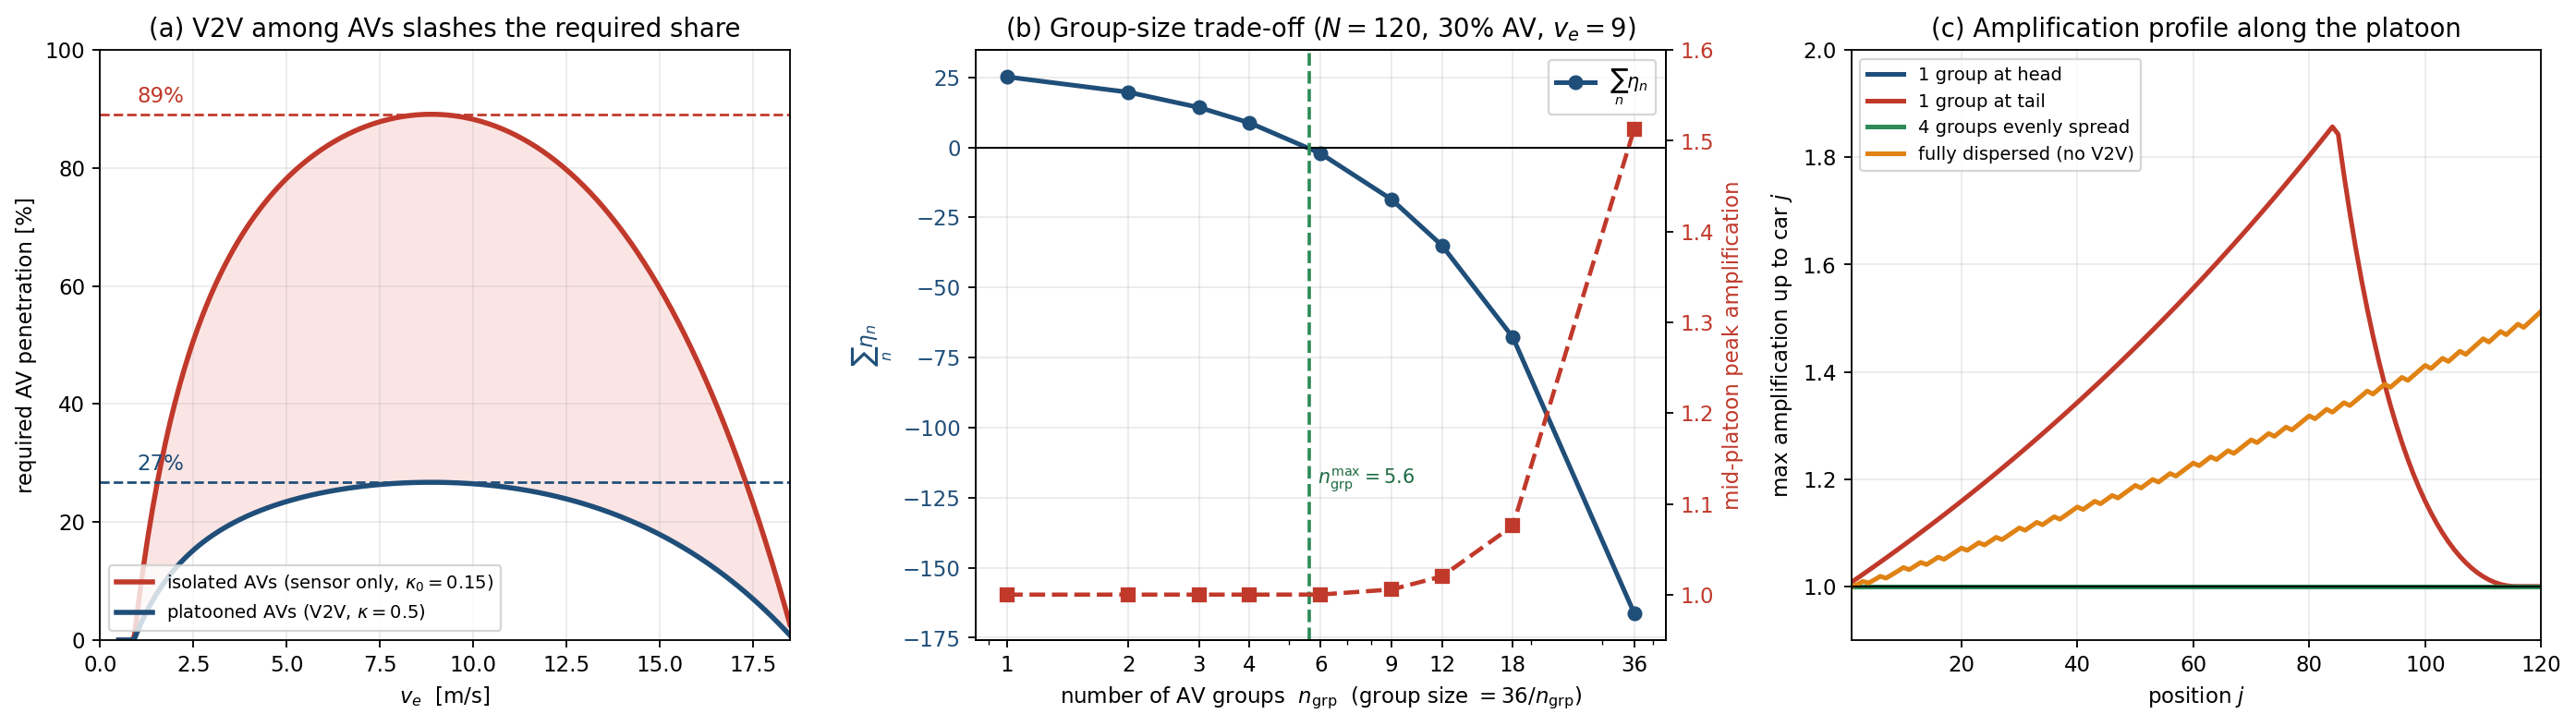
\includegraphics[width=\textwidth]{fig9.png}
\caption{Trade-off between the number of AV groups, penetration rate, and mid-route amplification.}
\label{fig:av-grouping}
\figurenote{Triple trade-off between total margin, spatial coverage, and disturbance source location in the AV grouping problem. The left figure compares the two lowest penetration rate curves: one for isolated AVs, which can only use radar to estimate gain ($\kappa_0$), and another for grouped AVs, which can use the full gain via V2V ($\kappa$); demand near the most unfavorable speed drops from approximately 89




\%




 to approximately 27\%, demonstrating that it is not the number of AVs itself that determines the payoff, but rather the number of AV-AV communication adjacency pairs formed. The middle figure shows a fixed number of 36 AVs, with the number of groups increasing along the horizontal axis: the blue total budget ($S_N$) decreases approximately linearly and crosses the zero line near $g_{\max}\approx5.6$, while the longest HDV segment shortens as the number of groups increases; This directly illustrates the conflict between Problem A (“Maximizing Total Margin”) and Problem B (“Improving Spatial Coverage Under Margin Constraints”) mentioned above. The right figure compares placing the same large AV group at the perturbation input end versus the propagation end: while the total gain at the end is the same for both, placing it at the end amplifies the signal to 1.857 before encountering the AV, indicating that identical total gains do not guarantee identical prefix exposure. This figure proves that if the objective is solely to maximize total margin, $g=1$ is optimal; if, in addition to maintaining the specified margin, one must also defend against perturbations at unknown locations, then the number of groups should be increased to the maximum feasible number and arranged approximately uniformly.
}
\end{figure}

\begin{tcolorbox}[keybox,title=\textbf{Two-Step Design Criteria for Optimal Grouping}]
\begin{enumerate}[leftmargin=1.6em,itemsep=3pt]
\item




Calculate the upper limit on the number of groups using Equation ~\eqref{eq:optimal-group-count} or the margin-included Equation ~\eqref{eq:robust-group-count}, ensuring the total stability budget is met first.







\item




 Select the maximum number of groups within the feasible range, and distribute the intervals between each group and the HDV as evenly as possible to minimize the longest consecutive HDV segment and the prefix peak.







\item




If only one large group can be placed, it should be located near the main disturbance input; in this example, placing it at the end of the queue would increase the midpoint peak by 85.7\%。
\item Increasing $\kappa_0$ reduces $\Delta\eta$, allowing for more numerous and more dispersed groupings; this indicates that improving AV has direct topological value for the quality of HDV acceleration estimates.







\end{enumerate}
\end{tcolorbox}

\section{Multi-Vehicle AV: From Scalar Transfer Functions to Transfer Matrices}
\sectionstudy{theory}{Multi-Vehicle AV: From Scalar Transfer Functions to Transfer Matrices}{swaroop1996,ploeg2014,feng2019}







\label{sec:heter-multileader}




In the case of nearest-neighbor feedforward, the $n$th vehicle depends only on the $n-1$th vehicle; therefore, a single scalar $G_n=Y_n/Y_{n-1}$ can be multiplied vehicle by vehicle. If the AV simultaneously receives acceleration broadcasts from $m$ vehicles ahead, $Y_n$ depends on $Y_{n-1},\ldots,Y_{n-m}$; in this case, there is no unique scalar input, and the state vector must be formed by combining $m$ consecutive vehicle disturbances.










\subsection{From Linearized Following Equations to Matrix Recurrence}










Considering Only Multiple Leading Vehicles




\textbf{Acceleration}Feedforward, while retaining the distance and relative velocity inputs provided by the nearest preceding vehicle. The linearized equation for a heterogeneous fleet is

\begin{equation}
\ddot y_n
=f_s^{(n)}(y_{n-1}-y_n)+f_v^{(n)}\dot y_n
+f_{v_l}^{(n)}\dot y_{n-1}
+\sum_{r=1}^{m}a_{n,r}\ddot y_{n-r},
\label{eq:heter-multi-time}
\end{equation}

where $a_{n,r}=0$ indicates that the $n$th vehicle has not received information from the $r$th preceding vehicle. Taking the Laplace transform with zero initial conditions and simplifying the term containing $Y_n$ yields

\begin{equation}
D_n(\lambda)Y_n
=\sum_{r=1}^{m}N_{n,r}(\lambda)Y_{n-r},
\qquad
D_n=\lambda^2-f_v^{(n)}\lambda+f_s^{(n)},
\label{eq:heter-multi-laplace}
\end{equation}

where

\begin{equation}
N_{n,1}=f_s^{(n)}+f_{v_l}^{(n)}\lambda+a_{n,1}\lambda^2,
\qquad
N_{n,r}=a_{n,r}\lambda^2\quad(r\ge2).
\label{eq:heter-multi-numerators}
\end{equation}

The first leading vehicle provides both a standard following stimulus and an acceleration broadcast, so $N_{n,1}$ contains three terms; more distant leading vehicles in this model provide only broadcast acceleration, so their numerators consist only of $a_{n,r}\lambda^2$.




Define

\begin{equation}
Z_n:=\begin{pmatrix}Y_n&Y_{n-1}&\cdots&Y_{n-m+1}\end{pmatrix}^{\!\mathsf T},
\end{equation}







Then the expression ~\eqref{eq:heter-multi-laplace} is equivalent to the accompanying matrix recursion

\begin{equation}
Z_n=M_n(\lambda)Z_{n-1},
\qquad
M_n(\lambda)=
\begin{pmatrix}
N_{n,1}/D_n&N_{n,2}/D_n&\cdots&N_{n,m}/D_n\\
1&0&\cdots&0\\
0&1&\ddots&\vdots\\
\vdots&\ddots&\ddots&0
\end{pmatrix}.
\label{eq:heter-multi-matrix}
\end{equation}







When $m=1$, $M_n$ degenerates into $G_n$ of $1\times1$; When $m=2$ occurs, the first line consists of the two fractions from the original text, and the second line simply shifts $Y_{n-1}$ one space to the right. The so-called “degeneration of the transfer function into a transfer matrix” essentially refers to the system’s spatial memory order increasing from 1 to $m$.





\subsection{Stability Conditions for Open Fleets and Ring Tracks}










The matrix representing the propagation of a disturbance from the source to the $j$th vehicle is an ordered product

\begin{equation}
\mathcal M_j(\lambda)=M_j(\lambda)M_{j-1}(\lambda)\cdots M_1(\lambda),
\qquad Z_j=\mathcal M_jZ_0.
\label{eq:heter-multi-prefix}
\end{equation}

For an open fleet, if it is required that no input combination be amplified, the sufficient condition of the induced second norm can be used

\begin{equation}
\sup_{\omega>0}\left\|\mathcal M_j(i\omega)\right\|_2\le1
\qquad \forall j.
\label{eq:heter-multi-open-condition}
\end{equation}

This condition is more conservative than specifying a particular input direction, but it covers any linear combination of $m$ historical vehicle disturbances.




For a ring track, the state vector must return to its original state after one lap; therefore







\begin{tcolorbox}[keybox,title=\textbf{Closing Equation for a Heterogeneous Circuit with Multiple Leading Vehicles}]
\begin{equation}
\det\!\left[\mathcal M_N(\lambda)-I_m\right]=0,
\qquad
\mathcal M_N=M_NM_{N-1}\cdots M_1.
\label{eq:heter-multi-ring}
\end{equation}
\end{tcolorbox}







All roots of the equation ~\eqref{eq:heter-multi-ring} should be found, excluding $\lambda=0$, which corresponds to a global translation. Since $M_n$ contains the denominator of $D_n$, the actual calculation should directly assemble the original $2N$-dimensional linear state matrix to compute the eigenvalues, or verify whether spurious roots are introduced after clearing the denominator; Scanning only $\|\mathcal M_N(i\omega)\|_2$ constitutes a small-gain screening and is not a complete necessary condition.










\subsection{Uniform Fleet Limit: Re-deriving the Multi-Lead Car Fourier Criterion}





If all vehicle parameters and weights are identical, let

\[
y_n(t)=\widehat y\,e^{\lambda t+ikn},
\qquad y_{n-r}=e^{-irk}y_n.
\]

Substitute this directly into equation ~\eqref{eq:heter-multi-time} to obtain

\begin{equation}
\underbrace{\left(1-\sum_{r=1}^{m}a_r e^{-irk}\right)}_{P_m(k)}\lambda^2
-\underbrace{\left(f_v+f_{v_l}e^{-ik}\right)}_{Q(k)}\lambda
-\underbrace{f_s\left(e^{-ik}-1\right)}_{R(k)}=0.
\label{eq:heter-multi-uniform-dispersion}
\end{equation}

This is precisely the multi-vehicle dispersion relation described in Chapter ~\ref{sec:multi}~. In other words, the transfer matrix does not introduce a separate theoretical framework: when the system is homogeneous, the spatial eigenvectors of the matrix are the Fourier modes; when the system is inhomogeneous, because $M_n$ varies with the vehicle, it is not possible to diagonalize them simultaneously using a single common wavenumber.




Let the zero-order and first-order moments of the weights be

\begin{equation}
m_0=\sum_{r=1}^{m}a_r,
\qquad
m_1=\sum_{r=1}^{m}r a_r.
\end{equation}

The long-wave expansion yields the necessary threshold

\begin{equation}
\frac{f_v^2-f_{v_l}^2}{2}\ge(1-m_0)f_s,
\label{eq:heter-multi-longwave}
\end{equation}

Therefore, the total gain $m_0$ determines whether the long wave can be stable; for a fixed $m_0$, shifting the weight toward a more distant leading vehicle increases $m_1$, which typically increases the finite wavelength margin. However, equation ~\eqref{eq:heter-multi-longwave} is only a necessary condition; it is still necessary to find the roots of all discrete $k$ in equation ~\eqref{eq:heter-multi-uniform-dispersion}.










\subsection{Why does the sorting order with multiple preceding vehicles potentially change even at the end?}





In the nearest-neighbor scalar case, $\prod_nG_n$ is commutative; once vehicle attributes are fixed, the total terminal gain is independent of the ordering. In scenarios with multiple leading vehicles, there is generally

\begin{equation}
M_AM_H\ne M_HM_A,
\end{equation}

because two input slots of a given AV may span different vehicle model boundaries. Therefore, swapping two vehicles will alter the eigenvalues and singular values of the full-lap matrix $\mathcal M_N$, and both the closed-loop roots and the total end-of-lap gain may change. The adjacent pair count $q$ and the scalar budget $S_N$ can only be used as nearest-neighbor approximations and cannot replace matrix-based determinations.










\begin{tcolorbox}[experimentbox,title=\textbf{Recommended Computational Workflow for Multi-Lead Vehicle Stability}]

First, specify the vehicle order and the set of lead vehicles that each AV can receive; then, construct each $M_n(i\omega)$ according to Equation ~\eqref{eq:heter-multi-matrix}, and scan all prefixes for the maximum singular value to evaluate in-path amplification; Subsequently, directly assemble the $2N$-dimensional state matrix to compute the rightmost eigenvalue and verify loop-track asymptotic stability; finally, perform a 1,800-second nonlinear IDM simulation using the same ordering. Only when the signs of the “matrix frequency domain, eigenvalues, and time domain” all match can the multi-leading-vehicle scheme be judged to be reliably stable.







\end{tcolorbox}

\section{Applicable Boundaries}
\sectionstudy{synthesis}{Applicable Boundaries}{talebpour2016,feng2019,stern2018}

\begin{itemize}[leftmargin=1.4em,itemsep=3pt]
\item \textbf{Heterogeneous $+$ Bidirectional Coupling}: Both the cascaded structure and the cyclic symmetry disappear; neither the scalar transfer function nor the spatial Fourier simplifications are applicable, so the eigenvalues of the $2N$-dimensional system must be calculated directly.







\item \textbf{Heterogeneous $+$ Delay}




: The per-vehicle transfer function can still be written (with $e^{-\lambda\tau_n}$ in both the numerator and denominator), and the per-vehicle criterion $\Psi_n(\omega)\ge0$ and the prefix product condition both hold as usual.







\item \textbf{Random Vehicle Order}




: If the arrangement cannot be controlled, one must either revert to the strict line-by-line stability under condition (ii) or establish a probabilistic bound for the random arrangement.







\end{itemize}

\section{Numerical Verification E6/E7: Formulation, Sorting, and AV Grouping}
\sectionstudy{experiment}{Numerical Verification E6/E7: Formulation, Sorting, and AV Grouping}{talebpour2016,feng2019,stern2018}










Take $N=120$, $v_e=9$ (m/s), and the AV proportion $30\%$. For E6, first assume that the AV’s $\kappa=0.5$ is a fixed attribute of the current vehicle, and only change the arrangement; for E7, then switch to a more realistic adjacent-pair rule: For AV–AV, use $\kappa=0.5$; for AV–HDV, use $\kappa_0=0.15$; for HDV, use $0$.










\begin{table}[htbp]
\centering
\small
\caption{Stability metrics for different formulations and configurations in E6/E7.}
\label{tab:e6e7-layouts}
\begin{tabular}{p{3.5cm}p{2.7cm}p{3.2cm}p{3.2cm}}
\toprule
\textbf{Layout} & \textbf{$\sum_n\eta_n$} & \textbf{Midpoint Peak} & \textbf{End Gain} \\
\midrule







Fixed Attributes, Uniform Distribution




&




 Same Total Budget




& $1.000$ & $1.0000$ \\







Fixed Attributes, HDV Continuously at the Front of the Fleet




&




 Same Total Budget




& $1.857$ & $1.0000$ \\







Adjacent Pair Rule, 4 Groups Evenly Distributed




& $+8.8$ & $1.000$ & $1.0000$ \\







Adjacent Pair Rule, Evenly Distributed Across 8 Groups




& $-44.4$ & $1.032$ & $1.0322$ \\







Adjacent Pair Rule, Distributed by Individual Vehicle




& $-166.2$ & $1.513$ & $1.5130$ \\
\bottomrule
\end{tabular}
\end{table}










Table ~\ref{tab:e6e7-layouts} presents five configurations under fixed vehicle attributes and the adjacent pair rule. The first two rows show that although the scalar product is the same, the prefix peak can still increase from 1.000 to 1.857; the last three rows show that once the effective gain is determined by AV–AV adjacency, increasing the number of groups also consumes the total budget, causing the 4-group configuration to remain stable while the 8-group and per-vehicle dispersion configurations become unstable.










\begin{tcolorbox}[experimentbox,title=\textbf{E7 Permeability and Number of Groups Results}]

When full forward propagation is fixed, the total budget threshold for long waves across the entire speed range is $26.7\%$. If a standalone AV can only use $\kappa_0=0.15$, this threshold increases to $89.1\%$. At a penetration rate of $30\%$, the closed-form solution yields $n_{\rm grp}^{\max}=5.6$; therefore, a maximum of 5 groups can be selected to first ensure the total budget. Subsequently, the specific arrangement must still be selected using the prefix peak. In the numerical table, 4 groups are stable while 8 groups become unstable, which is consistent with this upper bound.







\end{tcolorbox}

\begin{tcolorbox}[resultbox,title=\textbf{Verification Conclusions}]

When $G_n$ is fixed for each vehicle, the terminal product is independent of the ordering, but the prefix peak can increase from $1.000$ to $1.857$; When AV capability depends on the type of the preceding vehicle, the ordering also alters the AV–AV pair values in $q$, thereby changing the total budget as well. The engineering strategy is therefore a “two-step approach”: first, use $n_{\rm grp}^{\max}$ to ensure a stable total budget, then, within feasible limits, maximize the number of groups and minimize the length of consecutive HDV segments.







\end{tcolorbox}

\section{Specific Trajectory Results: Fixed Vehicle Attributes and Adjacent Pair Rules}
\sectionstudy{experiment}{Specific Trajectory Results: Fixed Vehicle Attributes and Adjacent Pair Rules}{ngsim2016,thiemann2008,krajewski2018}










Figure ~ \ref{fig:traj-s6} corresponds to E6:30\% The feedforward gain of the AV is fixed at $\kappa=0.5$; only the permutation is changed. The start-to-end ratios for a single AV cluster and a uniformly distributed group are $0.0228$ and $0.0219$, respectively, with negative slopes in the final segments, confirming that the final stability of the test loop is primarily determined by the formula; however, the peaks of the probe vehicles differ depending on the order of wave arrival, demonstrating the impact of sequencing on mid-course responses.










\begin{figure}[htbp]
\centering
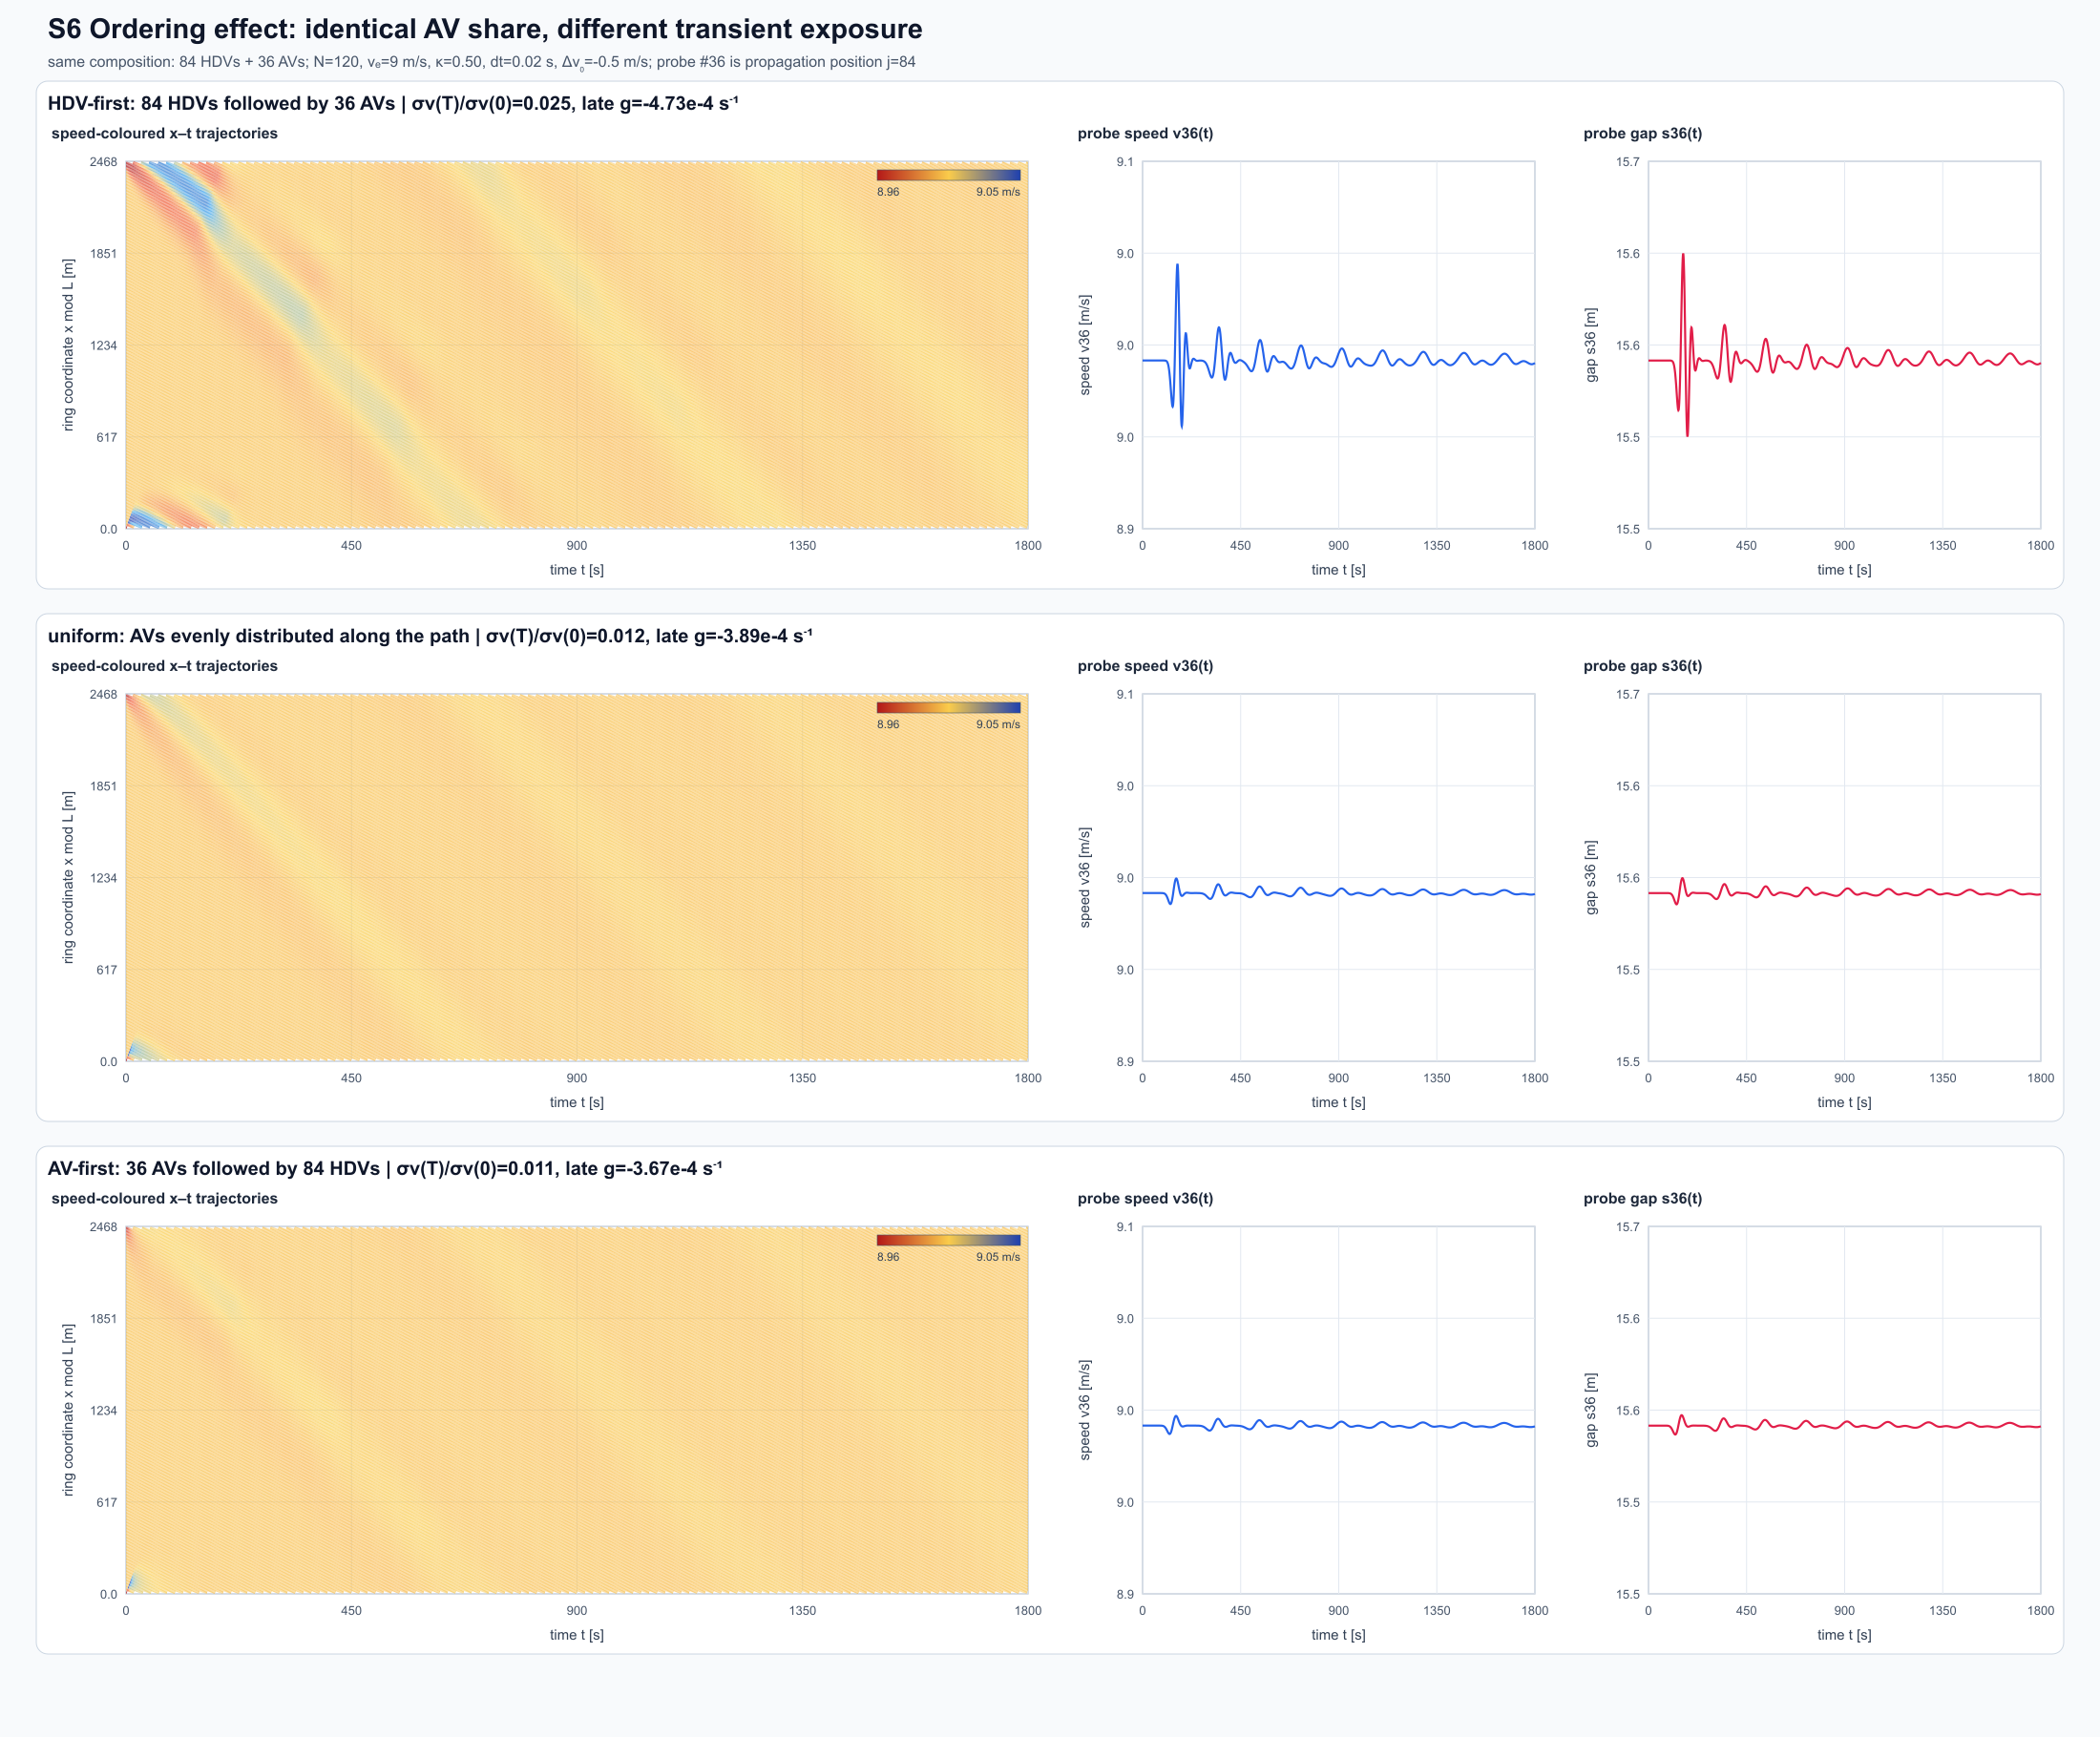
\includegraphics[width=\textwidth]{sim_s6_ordering_three.png}
\caption{S6: Time-domain comparison of three AV/HDV sequencing methods.}
\label{fig:traj-s6}
\figurenote{S6 isolates the sorting effect given the same vehicle model configuration. All three rows contain 84 HDVs and 36 AVs, utilizing the same impulses of $v_e=9$ m/s, $\kappa=0.5$, $\Delta t=0.02$ s, and $-0.5$ m/s; from top to bottom, the HDV is positioned at the leading end of the propagation path, in a uniformly interleaved arrangement, and with the AV at the entry end, respectively. The left column uses a uniform color scale, allowing for a direct comparison of the width and intensity of the color bands: when the HDV is at the leading end, the disturbance propagates significantly before encountering the AV; in the uniformly interleaved arrangement, damping segments are inserted continuously; and when the AV is at the front, the input is suppressed at the earliest possible stage. The two right-hand columns set the observation point at the vehicle according to $j=84$. The peak-to-peak velocity values ​​are approximately 0.0615, 0.00968, and 0.00685 m/s, respectively, while the peak-to-peak spacing values ​​are approximately 0.104, 0.0149, and 0.0110 m; these differences are far greater than those observed in the steady-state metrics. The final standard deviation ratios for all three schemes are below 0.026, demonstrating that the total budget is sufficient to ensure steady-state damping; however, the peak values ​​during the run differ by nearly an order of magnitude, showing that the ordering determines the velocity and spacing experienced by local vehicles. This figure thus provides comprehensive evidence regarding nonlinear trajectories, supporting the preliminary remarks and the interpretation of Figure ~\ref{fig:heter-order-budget}.


}
\end{figure}










Figure ~\ref{fig:traj-s7} corresponds to E7: When an AV follows an HDV, only $\kappa_0=0.15$ may be used; when following another AV, $\kappa=0.5$ is used. 30\% When AVs are dispersed one by one, the slope of the final segment is $+1.61\times10^{-3}$ s$^{-1}$, $\sigma_v(1800)/\sigma_v(0)=1.672$; After being divided into 4 uniform groups, the slope of the final segment becomes $-3.37\times10^{-4}$ s$^{-1}$, and the front-to-rear ratio decreases to $0.0273$. This provides direct time-domain evidence that “for the same permeability, simply altering the AV–AV adjacency structure is sufficient to reverse the stability sign.”










\begin{figure}[htbp]
\centering
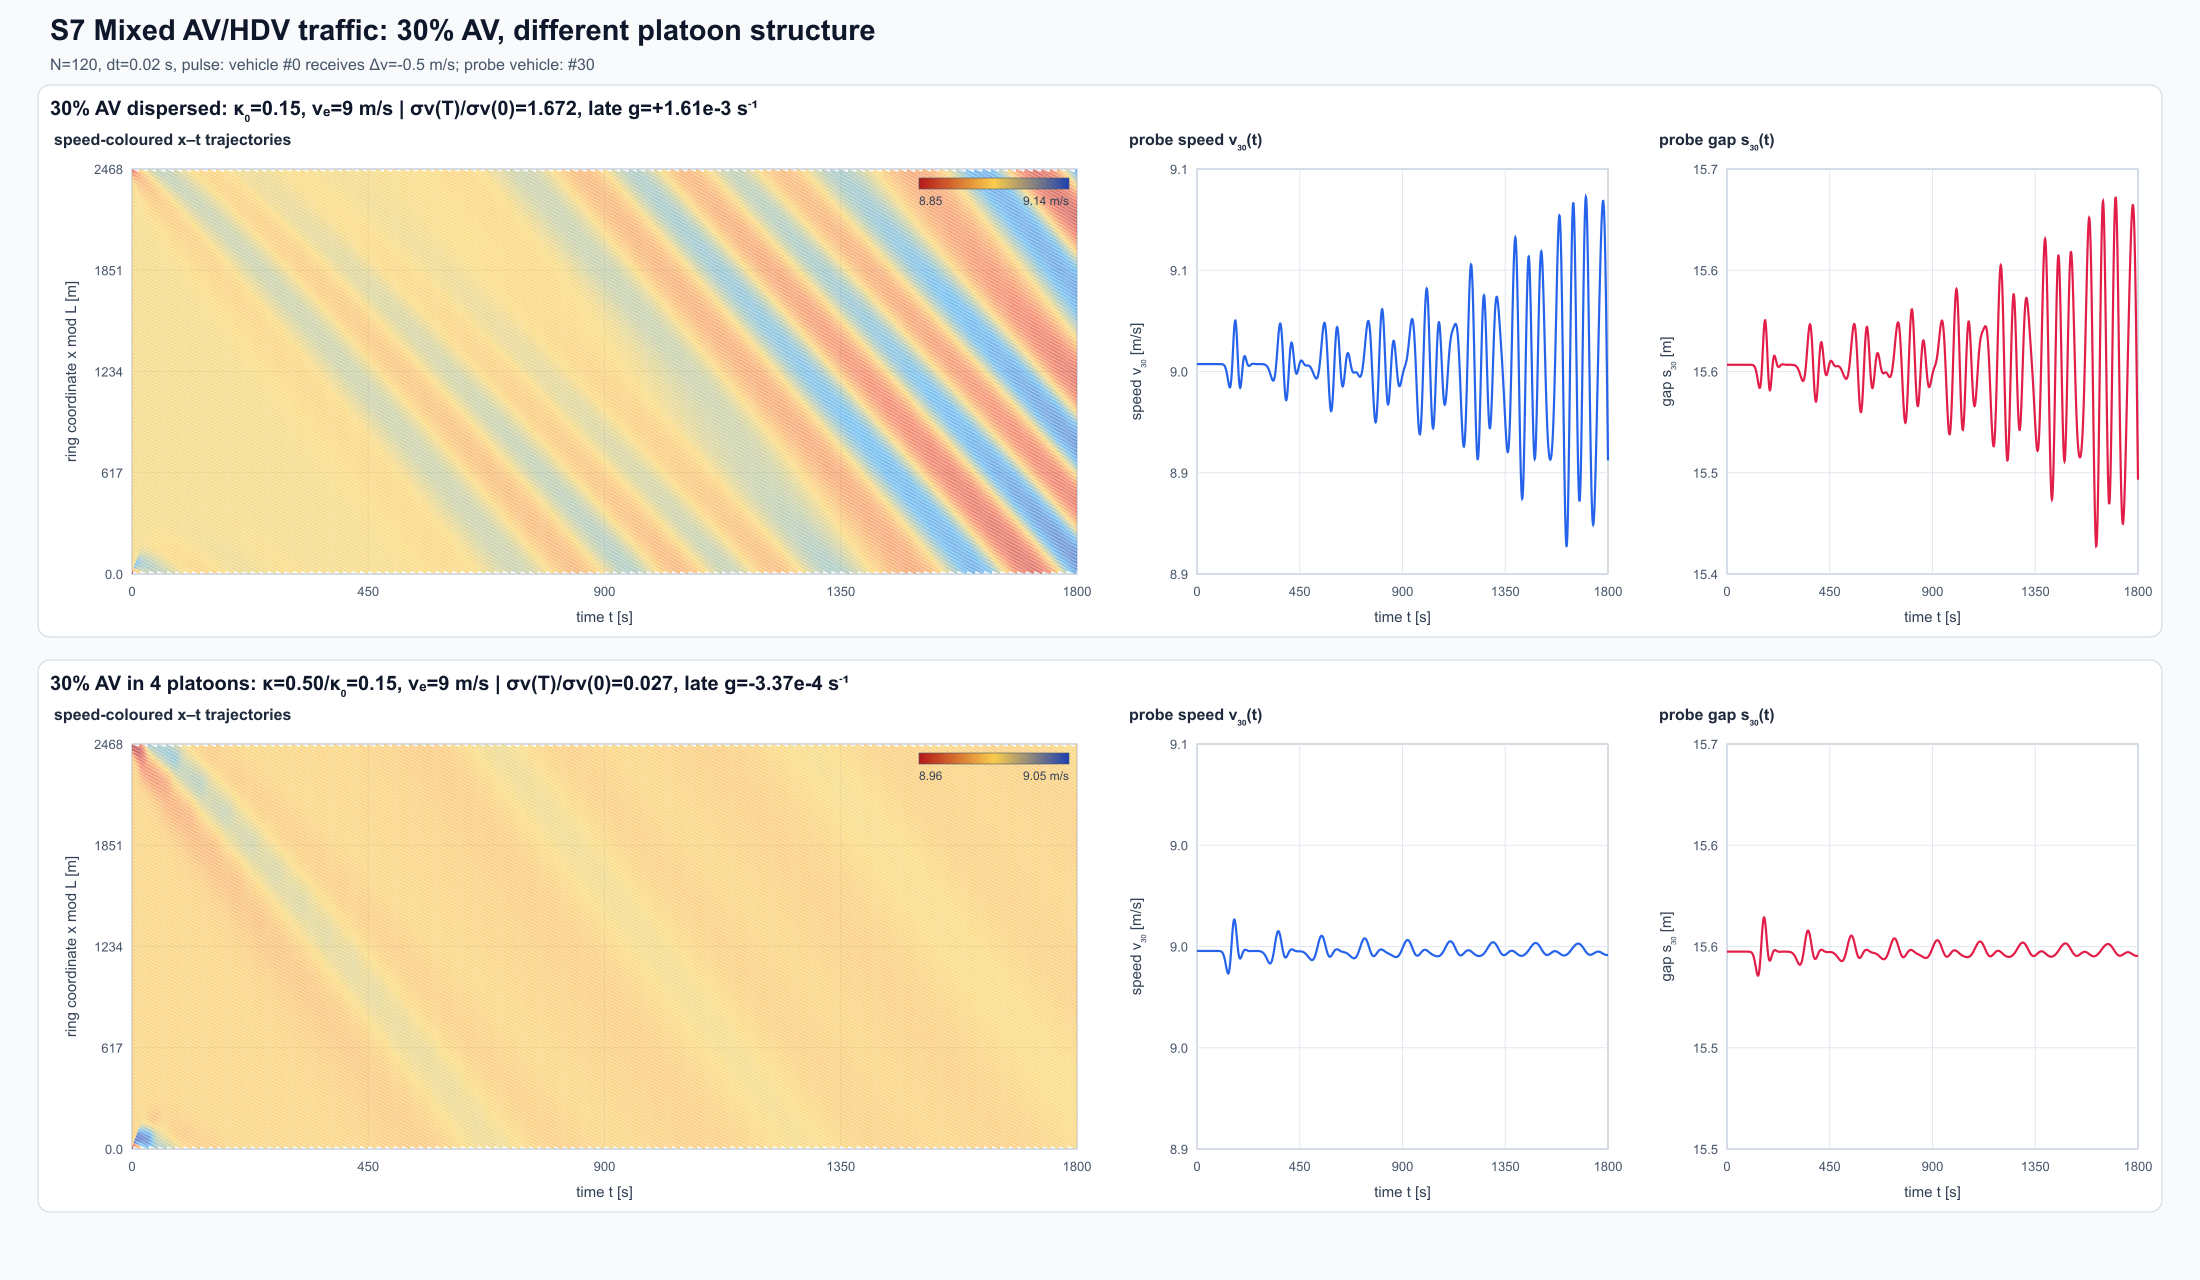
\includegraphics[width=\textwidth]{sim_s7_mixed_av.png}
\caption{S7: Trajectory comparison of AV formation structures.}
\label{fig:traj-s7}
\figurenote{S7 explanation same as 30 \% Why AV penetration rates may lead to opposite stability conclusions. In the upstream direction, AVs are dispersed one by one; the vehicle immediately ahead of each AV is mostly an HDV, so only radar-estimated gain $\kappa_0=0.15$ can be used; in the downstream direction, the same number of AVs are divided into 4 groups, and most vehicles within each group can use $\kappa=0.5$ via V2V. In the uplink, the position-time color bands deepen with each lap and form a continuous wave, with the speed and spacing amplitudes of the 30th vehicle increasing in sync; in the downlink, the color bands gradually narrow, and the two probe measurements return to equilibrium. Since the total number of vehicles, AV penetration rate, operating point, and perturbations are exactly the same, the difference can only stem from the actual available gain between adjacent AV pairs and cannot be attributed to “more AVs.” This figure demonstrates that penetration rate is merely a quantitative metric, while the communication topology is what translates that quantity into a stable budget; it also explains why mixed-traffic designs must report both arrangement and formation simultaneously.}
\end{figure}

\sectionwrapup{The stability of a heterogeneous vehicle fleet depends not only on vehicle models or AV penetration rates, but also on vehicle arrangements and communication relationships between adjacent vehicles. At the same AV penetration rate, dispersed and clustered arrangements can lead to opposite conclusions; macro-level ratio metrics cannot replace an examination of specific topologies.}

%==================================================================
\PART{VII}{From Micro-Level Linear Thresholds to Nonlinear Waves, Macro-Level Models, and Engineering Applications}

\chapter{Weak Nonlinear Stability Analysis of the Original IDM}
\label{sec:nonlinear}
\chapterguide{What Determines Amplitude and Waveform Beyond the Linear Threshold?}{




This chapter compares linear, weakly nonlinear, and strongly nonlinear problems, derives the Gardner–Burgers normal form, and explains the conditions of applicability and observational evidence for the Burgers, KdV, mKdV, and Gardner equations.
}










The linear theory discussed earlier answers the question of whether an infinitesimal perturbation initially grows or decays, but it does not explain why the perturbation does not diverge to infinity after growing, nor does it specify the final amplitude or the shape of the standing wave. This chapter focuses solely on the ~\ref{sec:idm}~ chapter’s




\textbf{original, uniform, unidirectional, delay-free IDM}




, without mixing feedforward, lookback, heterogeneity, and delay into the nonlinear reduction, to avoid combining higher-order terms from different mechanisms.










\section{The Purpose of Nonlinear Stability: What Is Missing Beyond the Linear Threshold}
\sectionstudy{theory}{The Purpose of Nonlinear Stability: What Is Missing Beyond the Linear Threshold}{komatsu1995,bando1995,ororsz2010}





“Nonlinear stability” encompasses at least two levels. The strict mathematical problem is: for a finite but nonzero initial perturbation, is the solution always bounded, does it return to a uniform equilibrium, and how large is the attractor of the equilibrium state? The weak nonlinearity problem is more specific: near a neutral curve, after retaining the lowest-order quadratic and cubic terms, how is linear growth modified by wave steepening, diffusion, and dispersion? This book provides a comprehensive discussion of the second level and explores the first level using finite-amplitude simulations, but does not mistake numerical phenomena for global proofs.




The linear spectrum provides only “tangential information” at the equilibrium state. On its own, it cannot answer the following four questions:







\begin{enumerate}[leftmargin=1.6em,itemsep=4pt]
\item \textbf{Where will the growth stop?}




 $\operatorname{Re}\lambda>0$ predicts only initial exponential growth; the actual velocity does not grow to infinity but instead forms a finite-amplitude run-and-stop wave, a stopping plateau, or wave peak coalescence.







\item \textbf{Is linear stability sufficient to withstand large perturbations?}




 $\operatorname{Re}\lambda<0$ only guarantees that sufficiently small perturbations will decay. A sudden stop may push the system out of the small-perturbation neighborhood, generating a very long nonlinear transient, or even causing it to fall into another attractor if a subcritical bifurcation exists.







\item \textbf{What is the final waveform?}




Linear modes are a superposition of sine waves; they cannot determine whether wave crests become sharper or whether wave troughs form a stationary plateau, nor can they provide relationships regarding the width of solitary waves or kinks.







\item \textbf{Can the controller still dampen the wave after congestion has already formed?} Linear stabilization indicates the presence of a recovery direction near the steady state; to determine whether the current stop-and-go behavior will truly disappear, it is also necessary to perform a direct integration using the current finite-amplitude state as the initial condition, or to study the attractor region of the controlled system.







\end{enumerate}

\begin{tcolorbox}[keybox,title=\textbf{Distinguishing in a Nutshell}]

Determined by linear analysis




\textbf{Initial direction, time scale, and dominant wavelength near the steady state}




; Determined by nonlinear analysis




\textbf{Threshold, saturation amplitude, waveform, propagation speed correction, and long-term state for finite-amplitude perturbations}




. The former is suitable for identifying the “threshold,” while the latter is suitable for explaining “what happens after the threshold.”







\end{tcolorbox}

\section{What Each of Linear, Weakly Nonlinear, and Strongly Nonlinear Analyses Addresses}
\sectionstudy{theory}{What Each of Linear, Weakly Nonlinear, and Strongly Nonlinear Analyses Addresses}{komatsu1995,bando1995,ororsz2010}

\begin{center}
\small
\captionof{table}{Division of Labor Among Linear, Weakly Nonlinear, and Fully Nonlinear Analyses.}
\label{tab:nonlinear-levels}
\begin{tabular}{p{3.1cm}p{5.2cm}p{5.4cm}}
\toprule
\textbf{Levels} & \textbf{Key Issues} & \textbf{Scope of Application / Output} \\
\midrule







Linear spectral analysis




&




 Whether Small Perturbations Grow and Which Wavelength Is Fastest




&




 $|r|\to0$; Outputs $\operatorname{Re}\lambda(k)$, $k^*$, and the neutral curve\\[4pt]

Schwache nichtlineare Reduktion




&






How waves steepen, propagate, and disperse near the neutral curve






&






Small, slowly varying waves of finite amplitude; derivation of amplitude equations such as Burgers, KdV, mKdV, or Gardner





\\

[4pt]

Full nonlinear simulation






&






Strong deceleration, approach to standstill, coalescence of wave crests, and long-term attractors






&






Direct IDM integration; yields trajectories limited in time and space, though typically without simple closed-form criteria






\\
\bottomrule
\end{tabular}
\end{center}
\tabletext{tab:nonlinear-levels}{






Questions and application areas for the three levels of analysis. The linear spectrum determines initial growth; the reduction to weak nonlinearity explains wave-shape evolution near the neutral line; while full simulation addresses strongly nonlinear phenomena such as stopping and the merging of wave crests.

}







Therefore, $\Phi<0$ merely describes the existence of a growth direction near the steady state; this does not imply that the velocity increases to infinity according to $e^{\sigma t}$. As the amplitude increases, the quadratic distance term, the free-stream term, and the IDM's approach term collectively alter the instantaneous restoring force; this causes the system to deviate from the linear tangent plane, results in a growth rate that varies with amplitude, and gives rise to a finite-amplitude wave.




A distinction must also be made between






\textbf{nichtlinearen Gleichungen}




und




\textbf{Conclusions regarding nonlinear stability}






. Simply formulating the complete IDM does not mean that the nonlinear stability analysis is complete; verifiable conclusions regarding nonlinear behavior can only be drawn after demonstrating the return to equilibrium for a given perturbation magnitude, calculating attractor boundaries, tracing bifurcation branches, or investigating the system's finite-amplitude responses.












\section{Common methods: What problems does each solve?}
\sectionstudy{theory}{Common methods: What problems does each solve?}{komatsu1995,bando1995,ororsz2010}

\begin{center}
\small
\captionof{table}{Common methods for nonlinear stability and their limitations.}
\label{tab:nonlinear-methods}
\begin{tabular}{p{3.0cm}p{5.0cm}p{5.7cm}}
\toprule
\textbf{Method} & \textbf{Core approaches} & \textbf{Most suitable problem formulations / limitations} \\
\midrule









Multi-scale nature / reduction to the center manifold






&






Introduction of "slow space-time" near the neutrality line; reduction of the discrete convoy to amplitude equations






&






Yields the Burgers, KdV, mKdV, and Gardner equations; allows for the explanation of corrections to amplitude width and wave speed, but applies only to small, slowly varying waves






\\[4pt]

Energie- oder Lyapunov-Verfahren




&






Construction of a monotonically decreasing function of time that provides an upper bound for the state norm






&






Provides rigorous local or global sufficient conditions; finding non-conservative energy functions is difficult for IDM systems with speed differences, asymmetric couplings, and saturation constraints






\\

[4pt]

Bifurcations and numerical continuation






&






Continuous tracking of equilibria, periodic waves, and their stability using density, time headway, or gain as parameters






&






Detection of supercritical/subcritical branches, coexisting attractors, and hysteresis; requires high computational effort and direct handling of the zero modes of the ring-track phase shift






\\

[4pt]

Direct simulation with finite amplitude






&






Sampling of perturbation amplitude, wavelength, and shape; full IDM via long-term integration






&






Closest match to the experimental platform; capable of handling standstill and wave-crest merging; provides evidence only for regions that have already been sampled and cannot replace a global proof





\\[4pt]

Datendiagnose




&






Derivation of the amplitude equation, the relationship between amplitude width and speed, as well as the hysteresis loop derived from the trajectories






&






For linking theory and experimental measurements; the results depend on the observation window, noise, mode separation, and the coverage of initial conditions





\\
\bottomrule
\end{tabular}
\end{center}
\tabletext{tab:nonlinear-methods}{






Five categories of methods: multiscale analysis, Lyapunov analysis, bifurcation continuation, direct simulation, and data diagnostics. This illustrates that no single tool can simultaneously provide a rigorous global proof, closed-form waveforms, and realistic responses to large disturbances; therefore, combined approaches are used in this book. }







This book employs the combination “






\textbf{Linear spectrum localization of the neutral point $\rightarrow$ Multiscale reduction mechanism $\rightarrow$ Full IDM simulation with limited amplitude for verification}






“. In this way, the readability of the analysis is preserved, and the reduction equations—valid only under $\varepsilon\ll1$—are prevented from being extrapolated into the strongly nonlinear regime characterized by repeated standstills.












\section{Typical traffic scenarios: Which level of analysis should be chosen?}
\sectionstudy{theory}{Typical traffic scenarios: Which level of analysis should be chosen?}{komatsu1995,bando1995,ororsz2010}

\begin{center}
\small
\captionof{table}{Typical traffic scenarios and recommended tools for nonlinear analysis.}
\label{tab:nonlinear-scenarios}
\begin{tabular}{p{3.5cm}p{4.7cm}p{5.5cm}}
\toprule
\textbf{Szenarien} & \textbf{Key questions} & \textbf{Recommended tools and metrics} \\
\midrule









Small, long-wavelength waves near the neutral axis






&






Does the wave decay slowly or grow slowly? Why does the waveform gradually become steeper?






&






Linear spectrum $+$ KdV–Burgers/Gardner; measurement of $\operatorname{Re}\lambda$, bandwidth, and phase velocity





\\

[4pt]

Walk-and-stop wave following linear instability






&






When does the exponential growth saturate, and what are the final stop frequency and amplitude?

&

Full long-term IDM simulation or continuation of the periodic wave; measurement of $v_{\min}$, $v_{\max}$, $\sigma_v$ and limit cycle





\\

[4pt]

Emergency braking under linear stability






&






Is there a finite-amplitude triggering threshold or an extremely long transient state?






&






Pulse amplitude scan, bidirectional parameter scan; measurement of energy in the final window, recovery time, and hysteresis






\\

[4pt]

Collision of two jam waves






&






Merging, competition, or mutual interpenetration of wave crests






&






Simulation of strong nonlinearity; tracking of wave crest position, mass, and merging time
\\

[4pt]

Activation of CACC following the formation of a traffic jam






&Can the controller return the existing wave—characterized by limited amplitude—to a steady state?






&






Simulation of the switching system / analysis of the basin of attraction; comparison of envelope slope and recovery time before and after the switch





\\

[4pt]

Including lane changes, noise, or communication packet loss






&






Continuous external disturbances; the deterministic equilibrium is no longer closed






&






Stochastic stability, mixed systems, or Monte Carlo methods; measuring probability distributions rather than individual trajectories






\\
\bottomrule
\end{tabular}
\end{center}
\tabletext{tab:nonlinear-scenarios}{






Key issues, recommended tools, and metrics for six traffic scenarios. This table helps the reader select the appropriate level of analysis based on disturbance amplitude, external inputs, and the presence of transitions, rather than applying the mKdV model to all phenomena.

}

\section{From the discrete IDM to the slowly varying amplitude equation}
\sectionstudy{model}{From the discrete IDM to the slowly varying amplitude equation}{treiber2000,treiberkesting2013}












Let us denote the spacing and velocity disturbances as

\begin{equation}
r_n=s_n-s_e,
\qquad
u_n=v_n-v_e .
\end{equation}

Instead of discarding higher-order terms, we perform a Taylor expansion of the full IDM around the equilibrium point:

\begin{equation}
\dot r_n=u_{n-1}-u_n,
\qquad
\dot u_n=\mathcal L_n(r,u)+\frac12\mathcal Q_n(r,u)+\frac16\mathcal C_n(r,u)+O(\|(r,u)\|^4),
\label{eq:nonlinear-taylor}
\end{equation}

Here, $\mathcal L_n$ represents the linear operator used previously, while $\mathcal Q_n$ and $\mathcal C_n$ capture the terms generated by the second- and third-order derivatives of the IDM, respectively. To consider only the slowly varying waves extending across many vehicles,

\begin{equation}
X=\varepsilon\bigl(n+c_1t\bigr),
\qquad
\mathcal T=\varepsilon^3t,
\qquad
c_1=V'(s_e),
\label{eq:slow-scales}
\end{equation}

Here, $\varepsilon$ simultaneously quantifies three "small quantities": the wavenumber $k=O(\varepsilon)$, the deviation from the neutral line, and the amplitude of the perturbation. The discrete shift occurs according to

\begin{equation}
R(X\pm\varepsilon,\mathcal T)
=R\pm\varepsilon R_X+\frac{\varepsilon^2}{2}R_{XX}
\pm\frac{\varepsilon^3}{6}R_{XXX}+\cdots
\label{eq:nonlinear-shift-expansion}
\end{equation}

expanded such that $R_X$ represents the long-wave shift, $R_{XX}$ the diffusion/anti-diffusion, and $R_{XXX}$ the discrete dispersion. The derivation can be understood in four steps:









\begin{enumerate}[leftmargin=1.6em,itemsep=3pt]
\item






$O(\varepsilon)$: Determination of the velocity $c_1=V'(s_e)$ in the moving coordinates, which matches the linear long-wave phase velocity;









\item






$O(\varepsilon^2)$: Obtaining the coefficient $c_2$, the sign of which corresponds to the stability sign for long waves;




\item

Next order: The second- and third-order Taylor terms yield $RR_X$ and $R^2R_X$ respectively, and the discrete shift yields $R_{XXX}$;









\item






By eliminating the modes that decay rapidly with velocity and applying solvability conditions to the slow modes, one obtains a single scalar amplitude equation. \end{enumerate}












The diffusion coefficient relative to the neutral line is expressed as $c_2=O(\varepsilon)$. When quadratic nonlinearity dominates, $r_n=\varepsilon^2R(X,\mathcal T)+\cdots$ is used; when the quadratic term degenerates and the cubic term dominates, $r_n=\varepsilon R(X,\mathcal T)+\cdots$ is used. After the stepwise elimination of modes with rapid velocity relaxation, the unified normal form on the long-wave center manifold is obtained as follows:









\begin{tcolorbox}[keybox,title=\textbf{The normalized form of the weakly nonlinear long waves of the original IDM}]
\begin{equation}
R_{\mathcal T}
+\alpha_2 R R_X
+\alpha_3 R^2R_X
=\nu R_{XX}-\beta R_{XXX}+\text{higher-order terms},
\label{eq:gardner-burgers}
\end{equation}
\end{tcolorbox}









Here, $\nu$ has the same sign as the linear long-wave coefficient $c_2$; $\nu>0$ represents dissipation and $\nu<0$ represents anti-diffusion; $\beta$ describes the dispersion of the discrete platoon of vehicles; $\alpha_2$ and $\alpha_3$ control the quadratic and cubic nonlinear steepness, respectively. While scaling the variables alters the values ​​of these coefficients, it does not affect whether they are zero or not, nor does it change their signs.












\begin{tcolorbox}[notebox,title=\textbf{Three conditions for the validity of the reduction}]

The following conditions must be met simultaneously: the operating point lies close to the neutral stability line, the perturbation amplitude is small, and the dominant wavelength is significantly larger than the spacing between the vehicles. If the vehicles have already come to a standstill, the spacing between adjacent vehicles is close to $s_0$, or the dominant mode involves only two to three vehicles per wave, then $\varepsilon$ is no longer small; consequently, the equation ~\eqref{eq:gardner-burgers} can only be interpreted qualitatively and is unsuitable for accurately predicting the amplitude.









\end{tcolorbox}












In the case where the spacing $R$ serves as the amplitude and normalization is applied according to the formula ~\eqref{eq:slow-scales}, the following dominant nonlinearity coefficient is derived from the equilibrium manifold:

\begin{equation}
\alpha_2=V''(s_e),
\qquad
\alpha_3=\frac12V'''(s_e).
\label{eq:nonlinear-coefficients}
\end{equation}

The linear dispersion coefficient is obtained by further expanding the dispersion relation to the first order:

\begin{align}
\lambda&=c_1\varepsilon+c_2\varepsilon^2+c_3\varepsilon^3+O(\varepsilon^4),
\qquad \varepsilon=-ik,\\
c_3&=\frac{(2c_1-f_{v_l})c_2-\frac12f_{v_l}c_1-\frac16f_s}{f_v+f_{v_l}}.
\label{eq:c3-general}
\end{align}

Exactly on the neutral stability line $c_2=0$, the above equation can be rearranged as follows:

\begin{equation}
c_3=\frac{f_s(2f_{v_l}-f_v)}{6(f_v+f_{v_l})^2}>0,
\qquad
\beta=c_3 .
\label{eq:c3-neutral}
\end{equation}

This demonstrates that if the dissipation term vanishes, the phase correction $O(k^3)$—resulting from the discrete vehicle structure—does not vanish simultaneously and can thus balance the nonlinear steepness. \section{When do Burgers, KdV, mKdV, and Gardner equations arise?}
\sectionstudy{theory}{When do Burgers, KdV, mKdV, and Gardner equations arise?}{komatsu1995,bando1995,ororsz2010}












The equation ~\eqref{eq:gardner-burgers} does not represent four mutually independent models, but rather a degeneration of a unified canonical form across different scales:









\begin{center}
\small
\captionof{table}{Dominant balances in the reduction to Burgers, KdV, mKdV, and Gardner equations.}
\label{tab:reduced-wave-equations}
\begin{tabular}{p{2.5cm}p{5.5cm}p{5.8cm}}
\toprule
\textbf{Reduktion} & \textbf{Dominant balance} & \textbf{Significance of the Traffic wave} \\
\midrule
Burgers & $R_{\mathcal T}+\alpha_2RR_X=\nu R_{XX}$ &






Nonlinearity leads to a steeper wave front, while normal diffusion leads to a broader one; frequent transition from triangular to shock-wave type





\\[4pt]
KdV & $R_{\mathcal T}+\alpha_2RR_X=-\beta R_{XXX}$ &






Balance between quadratic nonlinearity and dispersion; isolated pulses of the type $\operatorname{sech}^2$ can form near the neutral line





\\[4pt]
mKdV &




 $R_{\mathcal T}+\alpha_3R^2R_X=-\beta R_{XXX}$ und $\alpha_2=0$




&






Balance between cubic nonlinearity and dispersion; pulses or kink-antikink waves form depending on the sign of the coefficients





\\[4pt]
Gardner &






Simultaneous consideration of quadratic and cubic nonlinearity






&






If $\alpha_2$ is very small but not strictly zero, this is more reliable than "pure mKdV"





\\
\bottomrule
\end{tabular}
\end{center}
\tabletext{tab:reduced-wave-equations}{






The dominant terms of the four amplitude equations and their significance for traffic waves. Whether the quadratic term is degenerate and whether dissipation or dispersion dominates determines which reduced form should be used.


}












For example, for the dissipation-free KdV equation with $\alpha_2A/\beta>0$:

\begin{equation}
R(X,\mathcal T)=A\,\operatorname{sech}^2\!\left(\frac{X-U\mathcal T}{L}\right),
\qquad
U=\frac{\alpha_2A}{3},
\qquad
L=\sqrt{\frac{12\beta}{\alpha_2A}}.
\label{eq:kdv-soliton}
\end{equation}

This yields a verifiable relationship for the pulse width $L\propto|A|^{-1/2}$. The kink solution of the mKdV equation can be written as follows:

\begin{equation}
R(X,\mathcal T)=A\tanh\!\left(\frac{X-U\mathcal T}{L}\right),
\qquad
U=\frac{\alpha_3A^2}{3},
\qquad
L^2=-\frac{6\beta}{\alpha_3A^2},
\label{eq:mkdv-kink}
\end{equation}

However, it is suitable as a practical traffic wave only if $L^2>0$ holds and the states at both ends satisfy the conservation conditions. Therefore, merely "observing a steep wave front" is insufficient to substantiate the mKdV model; one must also verify that the quadratic coefficients are close to zero, as well as check the width relationship and the propagation speed.







\section{Typical nonlinear phenomena and their observable signs}
\sectionstudy{theory}{Typical nonlinear phenomena and their observable signs}{komatsu1995,bando1995,ororsz2010}

\begin{description}[style=unboxed,leftmargin=0pt,labelindent=0pt,labelsep=0.5em,itemsep=0.65em,font=\normalfont\bfseries\color{navy}]
\item[Waveform steepening]









The rising or falling edge of the wave becomes increasingly narrow, and higher-order harmonic oscillations intensify over time. This demonstrates that the propagation speed depends on the local amplitude, which is a direct manifestation of $RR_X$ or $R^2R_X$.
\item[Nonlinear saturation]Initially, $\ln|A(t)|$ follows a nearly linear path; subsequently, the slope decreases, and $\sigma_v$ fluctuates near a finite level. At this stage, it is no longer possible to approximate the entire profile using a fixed $\lambda$.












\item[Solitary waves and kinks]









An isolated wave is a local pulse; a kink connects two distinct plateaus. Assessment should not rely solely on shape; one should also examine how the propagation velocity changes as a function of $A$ or $A^2$, as well as how the scaling of $L\propto|A|^{-1/2}$ or $L\propto|A|^{-1}$ varies.












\item[Subcritical triggering and hysteresis]









Given identical parameters, small perturbations revert to uniform flow, whereas large perturbations sustain fluctuations over the long term; increasing density from the uniform state and decreasing density from the congested state result in different transition points. This must be confirmed through bidirectional scanning and a sufficiently long observation window.












\item[Amplitude dependence of recovery time]









Even if equilibrium is eventually restored, the process involving large perturbations can proceed significantly more slowly than a linear timescale would suggest. From a technical standpoint, the statements "fluctuations persist within 1800 s" and "mathematically speaking, never decaying" are not equivalent.




\end{description}







Figure ~\ref{fig:nonlinear-five-observables} translates the five aforementioned phenomena into measurable quantities that can be directly manipulated or read on the experimental setup. A distinction must be made here between two types of plots: plots (a), (b), (d), and (e) are derived from the full IDM numerical integration; plot (c) is a shape and scaling template for the reduced KdV/mKdV equation, intended to illustrate "how to verify" rather than to claim that the reference IDM has already produced a strict mKdV-type kink.

\begin{figure}[htbp]
\centering
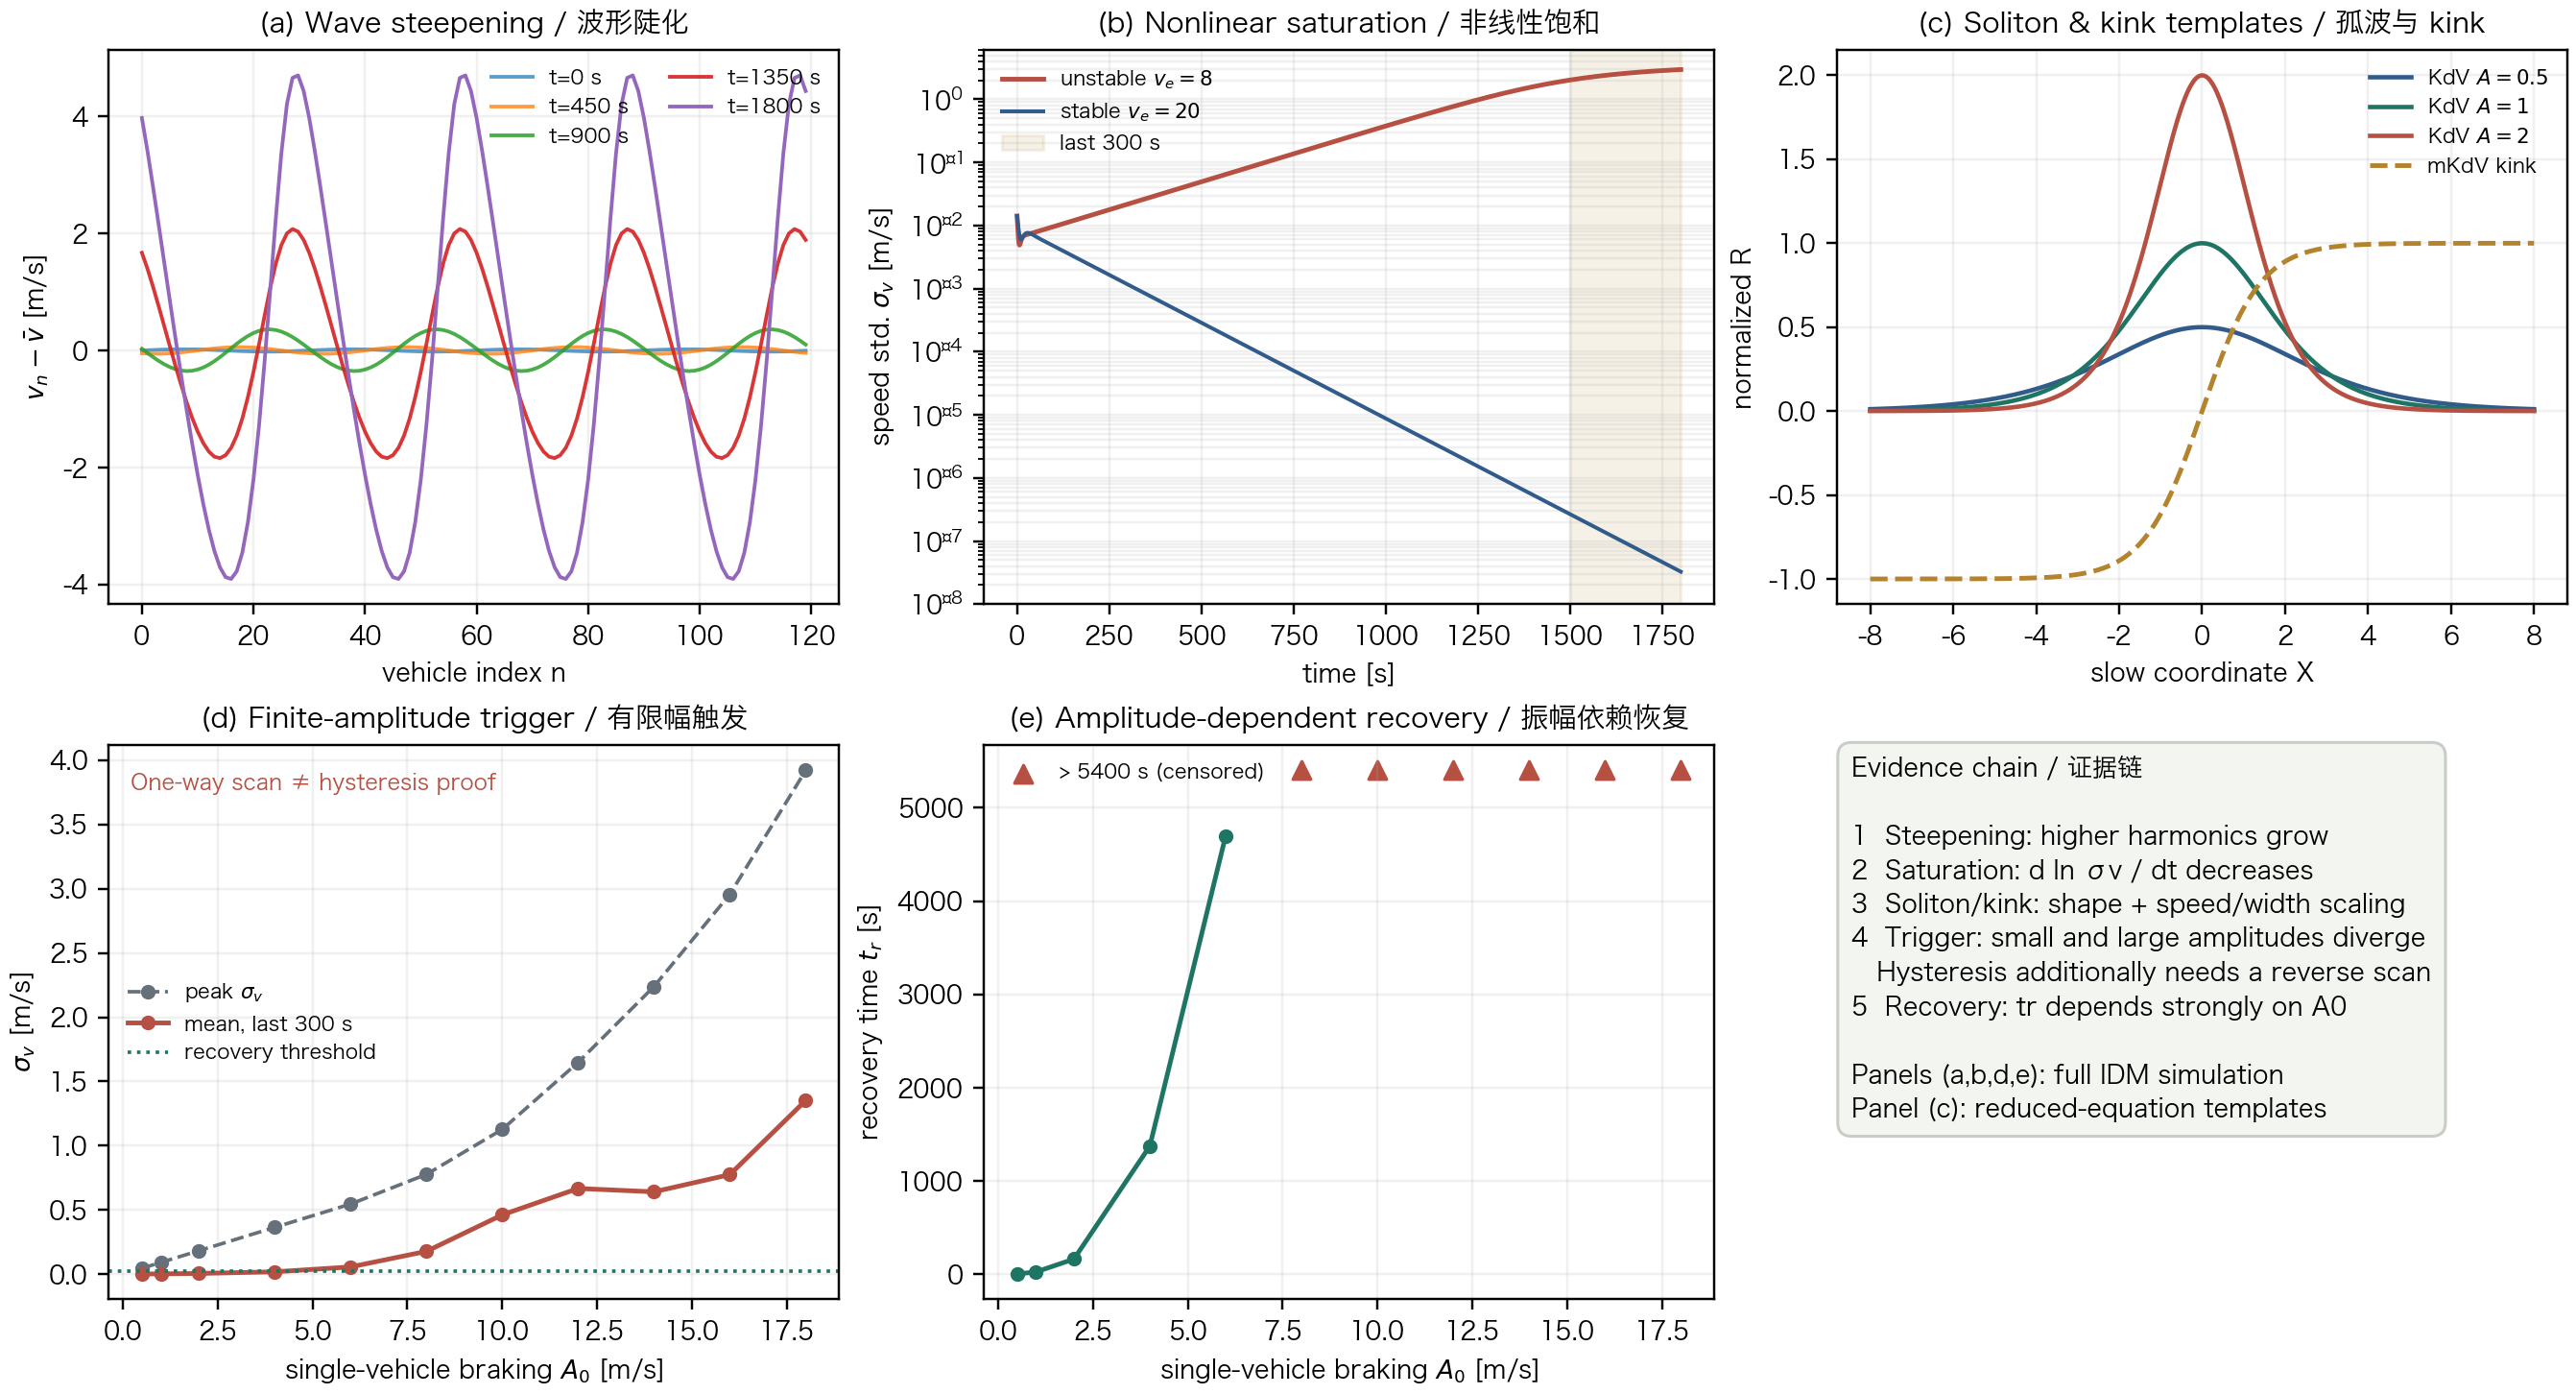
\includegraphics[width=\textwidth]{nonlinear_phenomena_observables.png}
\caption{Observable evidence for five types of nonlinear phenomena.}
\label{fig:nonlinear-five-observables}
\figurenote{Five types of stable nonlinear phenomena and the corresponding observational evidence required. The first image compares the fundamental wave with the higher harmonics: the sharper wave crests, broader troughs, and increased energy in the high-frequency range demonstrate that the waveform no longer follows a single linear mode. The second image contrasts the exponential envelope of the early phase with the plateau phase and the late phase, showing that a positive linear growth rate predicts only the initial amplification, whereas the final amplitude is determined by nonlinear saturation. The third image compares numerical waveforms with reduced templates from the KdV/mKdV class and assesses—based on propagation speed and shape stability—whether the isolated-wave approximation holds; the fourth image examines the amplitude of the initial perturbation to determine whether a finite-amplitude trigger threshold exists for linearly stable points. The fifth image shows the recovery time; Triangles indicate cases where the steady state was not yet reached within 5400 s (right-censoring), to avoid the status "not yet recovered" being erroneously interpreted as a precise time value. The figure as a whole demonstrates that linear stability provides insight only into the early trend under infinitesimal perturbations; waveforms, saturation, thresholds, and recovery rates must each be assessed using nonlinear indicators.}
\end{figure}

\begin{center}
\small
\captionof{table}{Metrics for five types of nonlinear phenomena and evidence from this calculation example.}
\label{tab:nonlinear-observables}
\begin{tabular}{p{2.7cm}p{4.4cm}p{6.1cm}}
\toprule
\textbf{Phenomenon} & \textbf{Metrics in the platform} & \textbf{Concrete results and correct conclusions from this calculation example} \\
\midrule


Steiler werdende Wellenform




&






Velocity profile; higher harmonic content $H=\sqrt{\sum_{m\ge8}|\hat v_m|^2}/|\hat v_4|$
&$H$ in $t=0,450,900,1350,1800$ are each $0,0.0034,0.0213,0.1091,0.1903$, demonstrating that the waveform gradually deviates from the pure sine mode.





\\

[3pt]

Nonlinear saturation






&






Instantaneous slope of the curve from $\log\sigma_v$ to $t$; mean value of the last window






&






$v_e=8$ m/s: $\sigma_v$ rises from $0.01414$ to $2.962$ m/s; the mean value over the last 300 s is $2.554$ m/s; the kink in the trailing section indicates that the constant linear growth rate no longer applies, but since slow growth is still observed at the end, this is simply referred to as "entering the saturation region."





\\[3pt]

Isolierte Welle/Knick




&






Scaling of waveform, propagation velocity, and width as a function of amplitude






&






The KdV model corresponds to $L\propto |A|^{-1/2}$, and the mKdV kink model corresponds to $L\propto |A|^{-1}$; since only the shape is present—without scaling or verification regarding coefficient degeneracy—it cannot be classified as an isolated wave or a kink.

\\

[3pt]

Limited-amplitude triggering / Hysteresis






&






Amplitude scan under the same operating conditions; bidirectional scan in the steady state / jammed state






&






At $\sigma_v<0.02$ m/s, the value in the last window is $A_0=0.5$ m/s $\sigma_v=8.8\times10^{-4}$ m/s, while $A_0=18$ m/s lies at $1.351$ m/s, demonstrating strong amplitude-dependent recovery; however, a unidirectional scan cannot demonstrate hysteresis; for this, a bidirectional scan with initial values ​​is still required.





\\

[3pt]

Recovery of the amplitude-dependent response






&






Time $t_r$ at which $\sigma_v<0.02$ m/s was first met for 300 s






&






$A_0=0.5,2,4,6$ m/s at $t_r=4,164,1374,4700$ s; at $A_0\ge8$ m/s, the threshold value was not yet reached after 5400 s, so only a loss on the right side can be reported.





\\
\bottomrule
\end{tabular}
\end{center}
\tabletext{tab:nonlinear-observables}{






Observable indications of steep waveforms, saturation, single-wave patterns, triggering at limited amplitude, and recovery time. Each row lists both the permissible conclusions and the statements that must not exceed certain limits, in order to prevent model decisions from being made solely on the basis of waveform similarity.


}

\begin{tcolorbox}[notebox,title=\textbf{How these five diagrams are used in the laboratory}]

After selecting the "Nonlinear Phenomena" tab, the five buttons correspond to the five types of evidence shown in Figure ~\ref{fig:nonlinear-five-observables}. Regarding waveform steepness, the point in time within the profile can be shifted; for single waves/kinks, the amplitude of the template can be shifted and the scaling of the amplitude width observed; The remaining three points show the IDM scan results, the specific values, and the limits for drawing conclusions regarding the same group leader. In this way, the reader can both recognize the phenomenon and determine which point represents a complete IDM verification, which merely corresponds to a form of the reduced equation, and which data are insufficient to demonstrate hysteresis.









\end{tcolorbox}

\section{Does the original IDM actually satisfy the mKdV conditions?}
\sectionstudy{model}{Does the original IDM actually satisfy the mKdV conditions?}{treiber2000,treiberkesting2013}












The equilibrium curve of the IDM is explicitly given by $s_e=s_e(v_e)$, so no repeated differentiation of the implicit function is required:

\begin{equation}
V'=\frac{1}{s_e'(v_e)},
\qquad
V''=-\frac{s_e''(v_e)}{[s_e'(v_e)]^3},
\qquad
V'''=\frac{3[s_e''(v_e)]^2}{[s_e'(v_e)]^5}-\frac{s_e'''(v_e)}{[s_e'(v_e)]^4}.
\label{eq:inverse-derivatives}
\end{equation}

Using high-precision central finite differences based on the reference parameters in this book, one obtains:









\begin{center}
\small
\captionof{table}{The weak nonlinearity coefficients of the reference IDM at three operating points.}
\label{tab:idm-nonlinear-coefficients}
\begin{tabular}{p{2.8cm}rrrr}
\toprule









Operating conditions






& $V'$ & $V''$ & $V'''$ & $c_3$ \\
 & [s$^{-1}$] & [m$^{-1}$s$^{-1}$] & [m$^{-2}$s$^{-1}$] & [veh$^3$/s] \\
\midrule









Lower neutral limit $v_e\approx0.91$






& $0.666665$ & $-5.12\times10^{-6}$ & $-9.49\times10^{-6}$ & $0.1938$ \\









Instability case $v_e=8$
& $0.660405$ & $-1.997\times10^{-3}$ & $-4.676\times10^{-4}$ & $1.8942$ \\









Upper neutral limit $v_e\approx18.61$

& $0.514195$ & $-1.474\times10^{-2}$ & $-4.13\times10^{-4}$ & $1.1446$ \\
\bottomrule
\end{tabular}
\end{center}
\tabletext{tab:idm-nonlinear-coefficients}{$V'$, $V''$, $V'''$ and the dispersion coefficient with two neutral boundaries and one instability point. The value of $V''$ at the lower boundary is very small but not strictly zero; consequently, the Gardner approximation is more appropriate, and one cannot unconditionally speak of a pure mKdV equation.


}

\begin{tcolorbox}[resultbox,title=\textbf{Concrete conclusions regarding the mKdV equation}]

The reference IDM does not satisfy the strict $V''(s_e)=0$ condition at either of the two neutral boundaries; therefore,






\textbf{the pure mKdV model cannot be regarded as a general nonlinear equation for the entire original IDM}






. At the lower boundary, $|V''|$ is very small; at a spacing amplitude of approximately $1$ m, the quadratic term $|V''R|$ and the cubic term $|V'''R^2/2|$ are of the same order of magnitude, making the Gardner equation suitable for describing the "near-mKdV" behavior at this point. At the upper boundary, the coefficient of the quadratic term is significantly non-zero, which corresponds more closely to the KdV/KdV-Burgers scenario. This numerical verification prevents the direct application of mKdV conclusions—drawn in the literature for specific optimal velocity functions—to the IDM without first verifying the underlying conditions. \end{tcolorbox}

\section{E11: 1800 s test with limited amplitude and interpretation of weak nonlinearity}
\sectionstudy{experiment}{E11: 1800 s test with limited amplitude and interpretation of weak nonlinearity}{komatsu1995,bando1995,ororsz2010}




\label{sub:nonlinear-exp}




$N=120$, $\Delta t=0.05$ s, RK4, and a time window of 1800 s are used. In the first group, a sinusoidal perturbation with $m=4$ and a velocity amplitude of $0.02$ m/s is introduced during the uniform equilibrium state; in the second group, under operating conditions of $v_e=20$ m/s—which are linearly stable against small perturbations—a single vehicle is briefly decelerated to $0.5$–$18$ m/s to examine recovery at limited amplitude.












\begin{figure}[htbp]
\centering
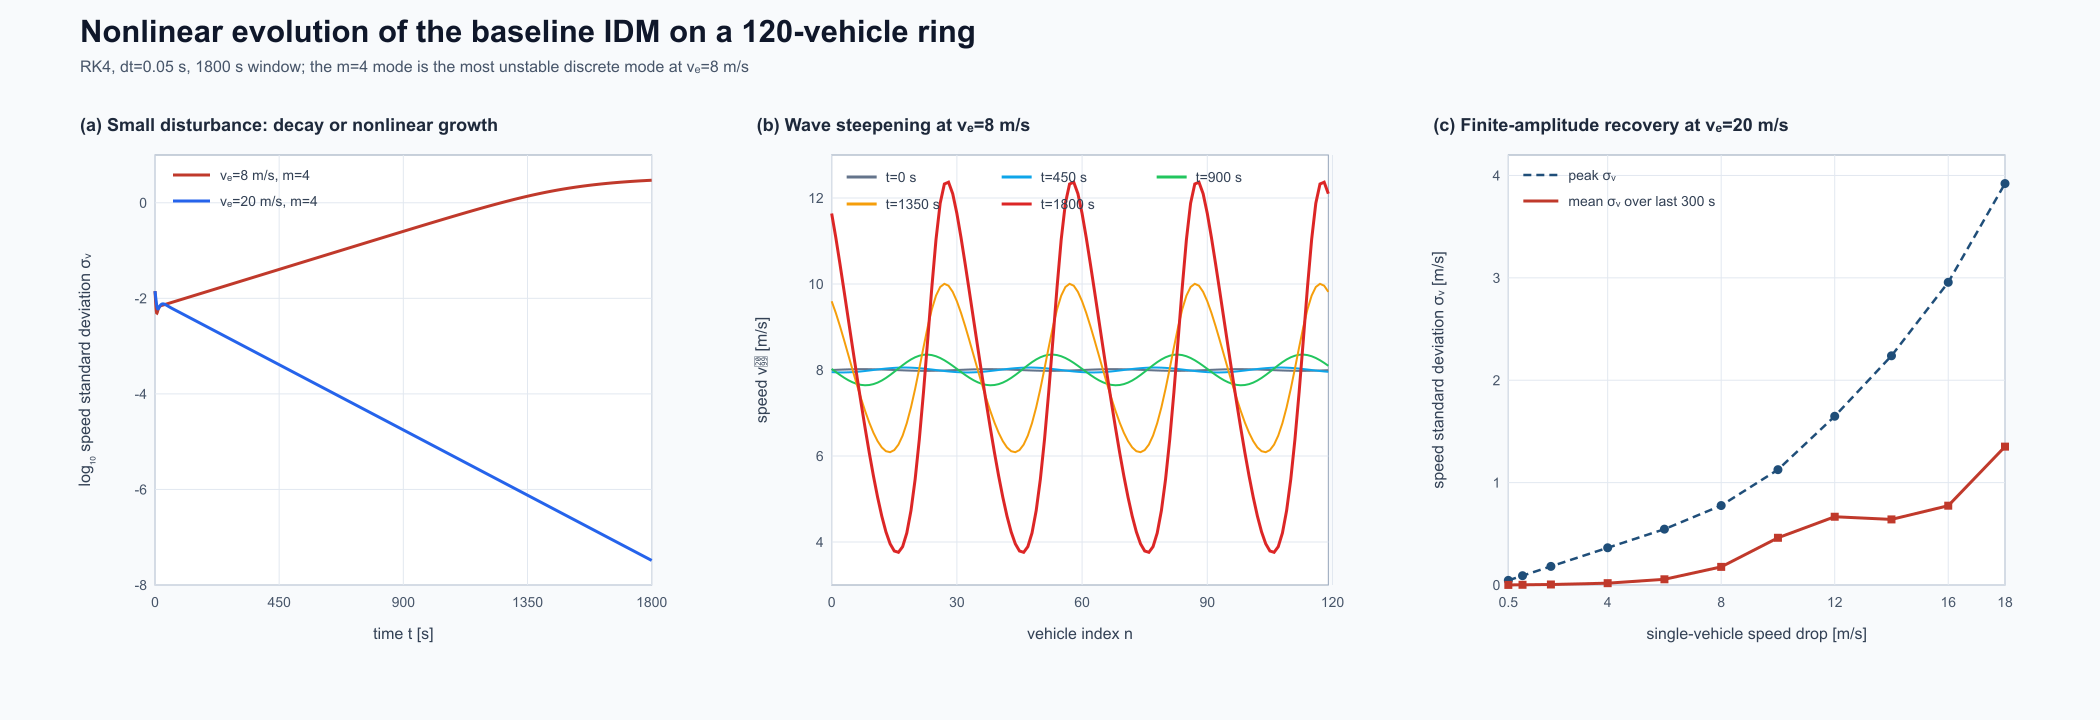
\includegraphics[width=\textwidth]{nonlinear_idm_experiment.png}
\caption{Nonlinear evolution and limited-amplitude response of the original IDM.}
\label{fig:nonlinear-idm}
\figurenote{Linear prediction of the original IDM and nonlinear result with limited amplitude. The figure on the left compares $v_e=8$ with the envelope of the dominant modes at 20 m/s: in the early stage of instability, the curve rises along a straight line with a positive linear slope, subsequently deviates from the exponential curve, and reaches a plateau with limited amplitude; In the stable state, it decays continuously, demonstrating that nonlinearity has not altered the initial stability characteristic regarding small perturbations. The middle figure displays spatial waveforms captured at various times during the unstable state: initially nearly sinusoidal, they subsequently exhibit asymmetric slopes and higher-order structures, indicating that mode interactions and waveform steepening have occurred. The right-hand figure shows a stepwise increase in the braking amplitude of a single vehicle at the nominally linear stability point, simultaneously plotting the peak values ​​of the entire process and the residual values ​​from the final 300 s; the separation of these two quantities illustrates that a large instantaneous response does not equate to sustained instability, whereas the sudden rise in residual values ​​signals a shift in the limited-amplitude attractor regime. This figure demonstrates that while linear theory reliably describes the early exponential phase, it cannot—on its own—provide information regarding the final amplitude of the decaying wave, the threshold for limited amplitude, or the recovery time.}
\end{figure}

\begin{center}
\small
\captionof{table}{E11 Limited-amplitude results after 1800 s for the original IDM.}
\label{tab:e11-nonlinear}
\begin{tabular}{p{4.0cm}p{4.3cm}p{5.4cm}}
\toprule
\textbf{Beispiel} & \textbf{Result after 1800 s} & \textbf{Explanation} \\
\midrule
$v_e=8$ m/s，$m=4$，$A_0=0.02$ m/s &




 $\sigma_v:0.01414\to2.962$ m/s; Endgeschwindigkeit $3.76$–$12.37$ m/s




&In the case of linear instability, $m=4$ is selected initially; subsequently, nonlinearity leads to a steeper waveform; in the final phase, no further adjustment using a fixed $\lambda$ is possible.





\\

[5pt]

$v_e=20$ m/s, identical small perturbation






& $\sigma_v:0.01414\to3.27\times10^{-8}$ m/s &






Agreement with $\Phi=+2.833\times10^{-3}>0$, recovery following a small perturbation.





\\

[5pt]

$v_e=20$ m/s, deceleration of a single vehicle by $18$ m/s.






&






Peak value over the entire duration: $3.921$ m/s; average over the last 300 s: $1.351$ m/s.






&






Linear stability is not synonymous with "rapid recovery within a limited timeframe"; large perturbations result in long transients, requiring an extension of the time window to distinguish the slow decay of persistent waves.





\\
\bottomrule
\end{tabular}
\end{center}
\tabletext{tab:e11-nonlinear}{






Three calculation examples: small perturbation under linear instability, small perturbation under linear stability, and a large impulse at the stability point. The results distinguish between the initial linear rise, the subsequent steepness of the waveform, and long transients associated with large perturbations. }

\begin{tcolorbox}[notebox,title=\textbf{What this series of experiments can and cannot prove}]

It proves that the linear spectrum






\textbf{the sign of the initial growth and the mode that appears first}






can predict, while the weak nonlinear term explains the subsequent steepness of the waveform and the amplitude-dependent evolution. It does not constitute proof of global Lyapunov stability, and the mere fact that residual fluctuations persist after 1800 s does not imply the existence of a subcritical second attractor. To investigate subcriticality, each pulse should be extended to at least several decay time constants, and bidirectional parameter sweeps should be performed starting from both the uniform and congested states to check for hysteresis.









\end{tcolorbox}

\section{E12: Diagram of the response with limited amplitude under linearly stable conditions}
\sectionstudy{experiment}{E12: Diagram of the response with limited amplitude under linearly stable conditions}{komatsu1995,bando1995,ororsz2010}












To distinguish between "linear stability" and "rapid recovery after large perturbations," only the instantaneous deceleration amplitude of vehicle no. 0 ($A_0$) was varied for the linearly stable operating states of $v_e=20$ m/s and $N=120$; the other parameters remain the same as in E11. The following table shows the standard deviation of the maximum speed throughout the process and the standard deviation of the average speed during the final 300 s:









\begin{center}
\small
\captionof{table}{E12: Peak values ​​throughout the process and residual values ​​in the final time window at different braking amplitudes.}
\label{tab:e12-finite-amplitude}
\begin{tabular}{rccccc}
\toprule
$A_0$ [m/s] & 0.5 & 4 & 8 & 12 & 18 \\
\midrule
$\max_t\sigma_v$ [m/s] & 0.0455 & 0.3636 & 0.7762 & 1.6483 & 3.9211 \\









Average of $\sigma_v$ [m/s] in the last 300 s

& 0.00088 & 0.01777 & 0.17705 & 0.66670 & 1.35145 \\
\bottomrule
\end{tabular}
\end{center}
\tabletext{tab:e12-finite-amplitude}{

Response of the same linearly stable operating point to five different deceleration amplitudes. Small pulses recover almost completely, whereas significant fluctuations persist in the final window for large pulses; this demonstrates that linear stability is not synonymous with rapid recovery from arbitrary amplitudes within a finite timeframe.


}












Small pulses decay almost completely within 1800 s, consistent with the conclusion regarding linear stability; as $A_0$ increases, the residual nonlinear fluctuations in the final window rise rapidly. Extending the integration period further to 5400 s and defining the recovery time as the moment when the condition $\sigma_v<0.02$ m/s is first met for 300 consecutive seconds yields

\begin{equation}
t_r(A_0=0.5,2,4,6\ {\rm m/s})=(4,164,1374,4700)\ {\rm s}.
\label{eq:nonlinear-recovery-times}
\end{equation}

At a value of $A_0\ge8$ m/s, this threshold was not reached within 5400 s, so this can only be noted as $t_r>5400$ s:
\textbf{crossed out on the right}as a result, and it must not be interpreted as $t_r=\infty$. Recalculating with $A_0=4,6$ m/s, $\Delta t=0.10$ s, and $0.05$ s yields $1374$ s and $4700$ s in both cases, demonstrating that the enormous recovery time observed here is not caused by the step size used. The reliable conclusion drawn from this scan is: "The recovery time and transient amplitude depend strongly on the perturbation amplitude," rather than: "Permanent congestion was detected at $A_0=18$ m/s." To draw the latter conclusion, the integration would need to be continued and the system checked for hysteresis using the parameters of the dynamic backward scan.












\begin{tcolorbox}[resultbox,title=\textbf{Linearity/non-linearity comparison of E11–E12}]
\begin{itemize}[leftmargin=1.4em,itemsep=3pt]
\item

$v_e=8$ m/s: The linear spectrum initially correctly predicts the growth of small perturbations and the dominant modes; the non-linear terms subsequently determine the steepness of the waveform and the saturation at finite amplitude.









\item






$v_e=20$ m/s, $A_0=0.02$ m/s: Linear theory is sufficient to predict the rapid recovery.









\item






$v_e=20$ m/s, large braking pulse: The stability sign does not change, yet linearization significantly underestimates the recovery time and peak values; the full IDM must be integrated directly.









\end{itemize}









Therefore, non-linear analysis serves not to "refute" linear criteria, but to supplement them regarding the range of applicability, the consequences of limited amplitudes, and the long-term state of attraction.









\end{tcolorbox}

\section{Praktische Reihenfolge der nichtlinearen Analyse}
\sectionstudy{synthesis}{Practical approach to nonlinear analysis}{komatsu1995,bando1995,ororsz2010}

\begin{enumerate}[leftmargin=1.6em,itemsep=4pt]
\item






First, the neutral boundary, $k^*$, and the linear time scale, $1/|\operatorname{Re}\lambda|$, are determined using the linear spectrum; if this level is incorrect, a reliable reference basis for the subsequent nonlinear fitting will be missing.









\item






Calculate $V''$, $V'''$, and $c_3$ near the neutral line: If $V''$ deviates significantly from zero, use KdV-Burgers; for $V''\approx0$, third-order terms are retained and the Gardner equation is primarily used; the pure mKdV equation is used only at the degeneracy points of $V''=0$.




\item

Verification of scaling laws using several sets of initial amplitudes: The growth rate in the linear phase should be independent of the amplitude; the KdV solitons should approximately satisfy $L\propto|A|^{-1/2}$; the mKdV kink should satisfy $L\propto|A|^{-1}$.









\item






As soon as the vehicle approaches a standstill, the distance $s_0$ is reached, or the acceleration enters the regime of strong nonlinearity, extrapolation using the weakly nonlinear equation is terminated and the system reverts to the full IDM simulation.









\end{enumerate}

%==================================================================
\sectionwrapup{Linear stability describes only the initial growth rate for infinitesimal perturbations; Furthermore, weakly nonlinear analysis provides information on waveform steepness, finite-amplitude saturation, and recovery time. For IDM, the recommended approach is to first determine threshold values ​​using the linear spectrum, then select the KdV-Burgers, mKdV, or Gardner reduction near these thresholds, and finally verify conclusions regarding finite amplitude via a fully nonlinear simulation.}

\chapter{Makroskopische Verkehrsflussmodelle}
\label{sec:macro-models}
\chapterguide{Where do the equations come from when vehicles are treated as a continuous fluid?}{






Based on the conservation of vehicle mass within a control volume, this chapter successively derives the closed-form structures of the LWR, PW, and ARZ models; explains the origins of the material derivative, relaxation, traffic pressure, viscosity, and generalized velocity; and outlines the solution procedure for the finite-volume method.
}The micro-model performs calculations for each individual vehicle ($x_n(t)$ and $v_n(t)$); the macro-model, on the other hand, describes traffic density ($\rho(x,t)$), spatially averaged speed ($v(x,t)$), and traffic flow at fixed road positions ($x$)

\begin{equation}
q(x,t)=\rho(x,t)v(x,t).
\label{eq:macro-fields}
\end{equation}

It approximates a discrete system of many vehicles as a continuous medium. Here, the question "Where do the macroscopic equations come from?" is answered first; the next chapter then addresses the question "Are the homogeneous solutions of these equations stable?"












\section{Common starting point: conservation of the number of vehicles within a fixed control volume}
\sectionstudy{theory}{Common starting point: conservation of the number of vehicles within a fixed control volume}{helbing2001,leveque2002,treiberkesting2013}












Consider a fixed road section $[x_1,x_2]$. If there are no on-ramps or off-ramps, the change in the number of vehicles

\begin{equation}
N(t)=\int_{x_1}^{x_2}\rho(x,t)\,\mathrm dx
\end{equation}

within the section can only be caused by the inflow from the upstream area and the outflow into the downstream area:

\begin{equation}
\frac{\mathrm d}{\mathrm dt}\int_{x_1}^{x_2}\rho\,\mathrm dx
=q(x_1,t)-q(x_2,t)
=-\int_{x_1}^{x_2}q_x\,\mathrm dx .
\label{eq:macro-integral-conservation}
\end{equation}

Since the control region is arbitrary, the integrated function must satisfy the condition

\begin{equation}
\boxed{\rho_t+q_x=0,\qquad q=\rho v.}
\label{eq:macro-continuity-intro}
\end{equation}

pointwise. By expanding the product, this can also be written as follows:

\begin{equation}
\rho_t+v\rho_x+\rho v_x=0.
\label{eq:continuity-expanded}
\end{equation}

The equation ~\eqref{eq:macro-continuity-intro} simply expresses that "vehicles do not appear or disappear out of thin air," yet it contains two unknown fields, $\rho$ and $v$, which is why an additional






\textbf{closure relation}






is required. The essential difference between LWR, PW, and ARZ lies precisely in how they close the velocity term.







\section{Basic diagram: Describes only the equilibrium, not the recovery process}
\sectionstudy{model}{Basic diagram: Describes only the equilibrium, not the recovery process}{helbing2001,leveque2002,treiberkesting2013}












When steady traffic reaches equilibrium, this can be represented using the velocity-density relationship and the traffic flow-density relationship as follows:

\begin{equation}
v=V(\rho),\qquad Q(\rho)=\rho V(\rho).
\label{eq:macro-fundamental-diagram-intro}
\end{equation}

Typically, $V'(\rho)<0$ applies, whereas $Q(\rho)$ initially rises and then falls. The fundamental curve answers the question "At what speed should one ultimately drive for a given density?" but provides no information on "how long recovery takes," nor does it independently determine the growth rate of the perturbation. One and the same $Q(\rho)$ can be combined with different relaxation times or pressure closure terms, resulting in vastly different dynamic stabilities. Later in this book, independent Greenshields curves are not used; instead, $V(\rho)$ is generated from the IDM equilibrium relationships, thereby aligning the macroscopic equilibrium state with the microscopic equilibrium state. \section{LWR: Conservation laws plus instantaneous equilibrium closure}
\sectionstudy{theory}{LWR: Conservation laws plus instantaneous equilibrium closure}{lighthill1955,richards1956,leveque2002}The central assumption of the LWR model is that local velocity exhibits no independent inertia; as soon as the density changes, the velocity immediately assumes the equilibrium value $v=V(\rho)$. Substituting this value into the vehicle conservation equation yields \cite{lighthill1955,richards1956}

\begin{equation}
\boxed{\rho_t+\bigl[Q(\rho)\bigr]_x=0,\qquad Q(\rho)=\rho V(\rho).}
\label{eq:lwr-model-derivation}
\end{equation}

Here, the subscript $x$ denotes the partial derivative with respect to road position, whereas $\bigl[Q(\rho)\bigr]_x$ does not.

$Q(\rho)$ is multiplied by $x$. Since density itself is $\rho=\rho(x,t)$, traffic flow is effectively a composite function

$Q(\rho(x,t))$. For smooth solutions, the chain rule is applied:

\begin{equation}
\frac{\partial}{\partial x}Q\!\left(\rho(x,t)\right)
=\frac{\mathrm dQ}{\mathrm d\rho}
\frac{\partial\rho}{\partial x}
=Q'(\rho)\rho_x.
\label{eq:lwr-chain-rule-detail}
\end{equation}

Therefore, the equation ~\eqref{eq:lwr-model-derivation} is equivalent to

\begin{equation}
\rho_t+Q'(\rho)\rho_x=0.
\label{eq:lwr-characteristic-form}
\end{equation}

Taking the parabolic fundamental model as an example,

\begin{equation}
Q(\rho)=v_f\rho\left(1-\frac{\rho}{\rho_j}\right),
\qquad
Q'(\rho)=v_f\left(1-\frac{2\rho}{\rho_j}\right),
\label{eq:lwr-example-flux}
\end{equation}

the propagation speed of the local density wave is

$c(\rho)=Q'(\rho)$. At low density $Q'>0$, the wave generally propagates downstream; on the high-density branch

$Q'<0$, the congestion wave can propagate upstream even while vehicles continue to move downstream. Here,

$Q'(\rho)$ equals






\textbf{die kinematische Wellengeschwindigkeit}

, not the vehicle speed $V(\rho)$.




This explanation can be formulated precisely using the characteristic curve. Along an arbitrary path $x=x(t)$, the total derivative of the density is

\begin{equation}
\frac{\mathrm d\rho}{\mathrm dt}
=\rho_t+\frac{\mathrm dx}{\mathrm dt}\rho_x.
\label{eq:lwr-density-total-derivative}
\end{equation}

Choosing

\begin{equation}
\frac{\mathrm dx}{\mathrm dt}=Q'(\rho),
\label{eq:lwr-characteristic-speed-detail}
\end{equation}

and applying equation ~\eqref{eq:lwr-characteristic-form} yields

\begin{equation}
\frac{\mathrm d\rho}{\mathrm dt}
=\rho_t+Q'(\rho)\rho_x=0.
\end{equation}

Therefore, the density value remains constant along the characteristic line with velocity $Q'(\rho)$. When the rear characteristic line catches up with the front one, the smooth wave compresses into a shock wave.












\begin{tcolorbox}[notebox,title=\textbf{Why must the conservation formula be maintained?}]

The transformation from $\bigl[Q(\rho)\bigr]_x$ to $Q'(\rho)\rho_x$ holds only for continuously differentiable density fields. At the shock wave, $\rho$ undergoes a jump, and $\rho_x$ is no longer an ordinary function; in this case, one must resort to

\[
\rho_t+\bigl[Q(\rho)\bigr]_x=0
\]




The conservation form, integrated across the shock wave in the sense of a weak solution. The shock speed connecting the left and right states $\rho_L,\rho_R$ is not simply replaced by a specific value of $Q'(\rho)$, but is determined by the Rankine-Hugoniot conditions.






























\end{tcolorbox}







Integrating across the shock using the pair of equations ~\eqref{eq:lwr-model-derivation} yields the Rankine–Hugoniot velocity

\begin{equation}
s_{\rm sh}
=\frac{Q(\rho_R)-Q(\rho_L)}{\rho_R-\rho_L}.
\label{eq:lwr-rh-model}
\end{equation}

Therefore, the LWR is well-suited for calculating queue boundaries, shock velocities, and rarefaction waves; however, “instantaneous equilibrium” means it lacks an independent velocity recovery mode and cannot generate a mechanism within the model to amplify perturbation waves from cell to cell.










\subsection{Manual Example W02: How to Update Four LWR Grids in Two Steps}


\label{sub:worked-lwr}




First, let’s demonstrate the finite-volume update using a simple triangular diagram that’s easy to calculate by hand:

\begin{equation}
Q(\rho)=\min\{30\rho,\;5(0.15-\rho)\},
\label{eq:w02-triangular-fd}
\end{equation}

Here, density is measured in veh/m and flow rate in veh/s. The critical density is

$21.4286$ veh/km, and the capacity is $0.642857$ veh/s, which is equivalent to $2314.3$ veh/h.

Consider four cells, $\Delta x=500$ m, and $\Delta t=5$ s, and fix the densities of the left and right virtual cells at

$10$ and $50$ veh/km, respectively. The initial value is

\begin{equation}
\bm\rho^0=(10,20,50,50)\ {\rm veh/km}.
\label{eq:w02-initial}
\end{equation}

For a triangular mesh, the Godunov flux can be written as

\[
\widehat Q(\rho_L,\rho_R)=\min\{D(\rho_L),S(\rho_R)\},
\]

where $D$ is the upstream demand and $S$ is the downstream supply. The first-step fluxes across the five interfaces from left to right are

\begin{equation}
\widehat{\bm Q}^{\,0}=(0.3,0.3,0.5,0.5,0.5)\ {\rm veh/s}.
\label{eq:w02-first-flux}
\end{equation}

For example, the inflow to the second cell is $0.3$ and the outflow is $0.5$ veh/s, so

\begin{align}
\rho_1^1
&=0.020-\frac{5}{500}(0.5-0.3)
=0.018\ {\rm veh/m}
=18\ {\rm veh/km}.
\label{eq:w02-cell-update}
\end{align}

After all four units are updated simultaneously,

\[
\bm\rho^1=(10,18,50,50)\ {\rm veh/km}.
\]

Recalculate the interface flux using $\bm\rho^1$, then proceed one step further to obtain

\begin{equation}
\bm\rho^2=(10,16,50,50)\ {\rm veh/km}.
\label{eq:w02-second-update}
\end{equation}

The second unit decreases by 2 veh/km every 5 s because it continuously receives vehicles at a rate of $0.3$ veh/s,


Instead, vehicles are supplied to the congested area using $0.5$ veh/s. The entire update uses only “inflow minus outflow,” which is precisely

the discrete interpretation of the conservation form; $Q'(\rho)\rho_x$ cannot be used directly for central differencing at the jump points.










\subsection{Teaching Example M06: Verifiable Shock Waves on the IDM Basic Diagram}







\label{sub:m06-lwr}




W02 uses a triangular grid for manual calculations; M06 reverts to the IDM balanced basic grid described in this book. On a 4-km road,

the left and right density values are set to $20$ and $60$ veh/km, respectively. The Rankine–Hugoniot conditions yield

\begin{equation}
c_{\rm sh}=\frac{Q(60)-Q(20)}{60-20}
=-2.42536\ {\rm m/s}.
\label{eq:m06-shock}
\end{equation}

Using $\Delta x=25$ m and $\Delta t=0.5$ s, the Godunov method was applied for 60 s,

and $-2.29167$ m/s was obtained by averaging the density values; the absolute error is $0.13370$ m/s,

which is less than $\Delta x/60=0.4167$ m/s—the value corresponding to one grid cell.










\begin{figure}[htbp]
\centering
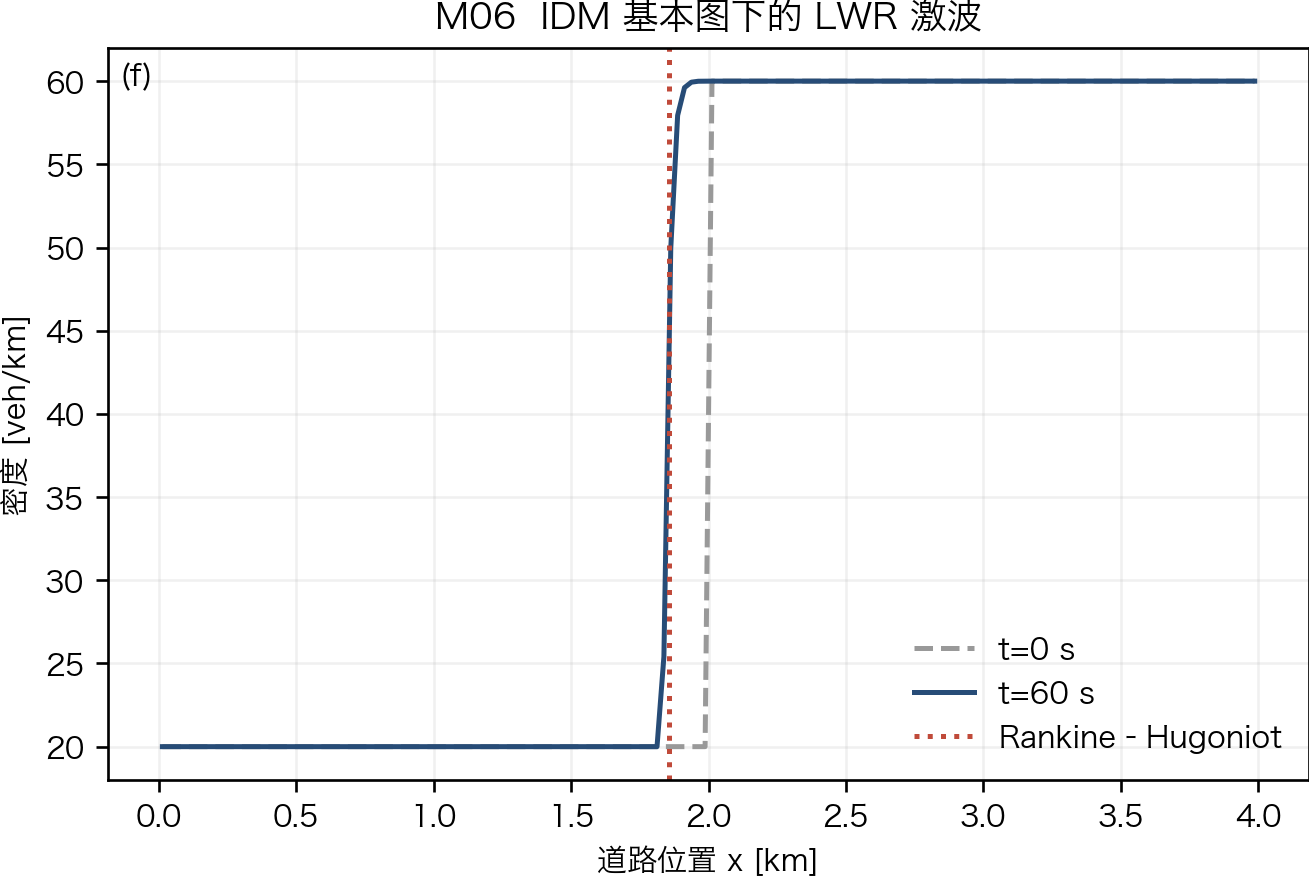
\includegraphics[width=0.84\textwidth]{mini_example_m06.png}
\caption{M06: LWR shock wave under the IDM reference model.}
\label{fig:m06-lwr}
\figurenote{M06 Verifies conservation updates and shock wave velocity using the smallest LWR grid. The initial road consists of two different IDM equilibrium density states; the finite volume method updates at each interface by subtracting outflow from inflow. The blue curve shows the numerical density profile at 60 s for various grid resolutions, while the red curve is independently predicted by the Rankine–Hugoniot equation $c_s=(q_R-q_L)/(\rho_R-\rho_L)$. As the mesh is refined, the numerical transition zone narrows around the same red location, indicating that diffusion primarily stems from discrete fluxes, while the shock propagation speed is correctly preserved by vehicle conservation. The calculated $c_s<0$ shows that the density discontinuity moves upstream in fixed road coordinates, while the vehicles themselves continue to travel downstream at a positive velocity. This figure demonstrates that the reverse congestion wave observed in the macroscopic spatiotemporal diagram does not require the assumption that vehicles are reversing, but rather represents the motion of a conserved boundary between different density states.}
\end{figure}

\section{PW: Adds inertia, pressure, and relaxation to velocity}
\sectionstudy{theory}{PW: Add inertia, pressure, and relaxation to velocity}{payne1971,daganzo1995,jin2003}










To ensure that vehicle velocity does not jump instantaneously to $V(\rho)$, $v$ must also be treated as a state. The structure of PW is indeed inspired by the one-dimensional compressible Euler/Navier–Stokes equations, but it does not represent the actual conservation of mechanical momentum of the vehicle; rather, it is a




\textbf{behavioral closure under a fluid analogy}。

\subsection{Material derivative: the actual acceleration observed relative to the vehicle}





Suppose the trajectory of a vehicle is $x=x(t)$, and

\begin{equation}
\frac{\mathrm dx}{\mathrm dt}=v(x(t),t).
\end{equation}

the actual velocity experienced by the vehicle is the composite function $v(x(t),t)$. The chain rule yields

\begin{align}
\frac{\mathrm d}{\mathrm dt}v(x(t),t)
&=\frac{\partial v}{\partial t}
+\frac{\mathrm dx}{\mathrm dt}\frac{\partial v}{\partial x}\\
&=v_t+vv_x.
\end{align}

Therefore, the change in velocity observed by an observer moving with the traffic flow is the material derivative

\begin{equation}
\frac{\mathrm Dv}{\mathrm Dt}=v_t+vv_x.
\label{eq:material-derivative}
\end{equation}

Here, $v_t$ represents the local time variation observed by a fixed detector, while $vv_x$ represents the convective variation caused by the vehicle entering regions with different velocities. Even if the velocity field does not vary with time ($v_t=0$), when a vehicle enters a downstream region where the velocity gradually decreases ($v_x<0$), $\mathrm Dv/\mathrm Dt=vv_x<0$ still applies, and the vehicle will actually decelerate.










\subsection{Where does the equation structure come from: Correspondence with the one-dimensional compressible NS equations}










The mass and momentum equations for a one-dimensional compressible fluid can be written as


\begin{subequations}
\label{eq:ns-analogy}
\begin{align}
\rho_t+(\rho u)_x&=0,\\
(\rho u)_t+(\rho u^2+p)_x
&=(\mu u_x)_x+\rho f,
\end{align}
\end{subequations}


Here, $u$ represents the fluid velocity, $p$ represents the pressure, $\mu$ represents the dynamic viscosity, and $f$ represents the external force per unit mass. Expanding Equation (2) using Equation (1) and eliminating the mass conservation term yields

\begin{equation}
u_t+uu_x
=-\frac{1}{\rho}p_x
+\frac{1}{\rho}(\mu u_x)_x+f.
\label{eq:ns-nonconservative}
\end{equation}

In the vicinity of a locally uniform density, $\mu/\rho$ can be combined into an approximate constant $\nu$, and the viscous term on the right-hand side can be written as $\nu u_{xx}$. PW replaces $u$ with traffic velocity $v$, replaces mechanical pressure $p$ with traffic pressure $P(\rho)$, and then replaces “external force” with the relaxation effect caused by the driver actively maintaining a balanced speed. This results in the structure \cite{payne1971}: “material acceleration $=$, relaxation $-$, pressure gradient $+$, viscosity”:

\begin{equation}
\boxed{
\frac{\mathrm Dv}{\mathrm Dt}
=\frac{V(\rho)-v}{\tau}
-\frac{1}{\rho}P_x
+\nu v_{xx}.}
\label{eq:pw-force-balance}
\end{equation}

If viscosity and relaxation are removed, the structure more closely resembles the compressible Euler equations; when viscosity is retained, it approximates the Navier–Stokes equations; and only after adding the relaxation term does it become the traffic flow PW model.










\subsection{Traffic Implications and Sources of Approximations for the Three Types of Effects}

\paragraph{Relaxation: Active acceleration or braking.}


The simplest recovery law is

\begin{equation}
\frac{\mathrm dv}{\mathrm dt}
=\frac{V(\rho)-v}{\tau}.
\label{eq:pw-relaxation-alone}
\end{equation}

If $\rho$ is treated as a constant for a short period of time, then

\begin{equation}
v(t)=V(\rho)+\bigl[v(0)-V(\rho)\bigr]e^{-t/\tau}.
\end{equation}

Therefore, when $v<V(\rho)$ occurs, the vehicle accelerates; when $v>V(\rho)$ occurs, the vehicle decelerates; and $\tau$ represents the time scale for deviation decay. This term is not a force inherent to the standard NS equations, but rather an additional active acceleration/braking term introduced to account for traffic behavior.










\paragraph{Traffic pressure: anticipation of the density gradient ahead.}







Assume the driver observes the density at a distance of $d$ ahead. Perform a Taylor expansion for a smooth field:

\begin{align}
\rho(x+d,t)
&=\rho(x,t)+d\rho_x+O(d^2),\\
V\!\left(\rho(x+d,t)\right)
&=V(\rho)+dV'(\rho)\rho_x+O(d^2).
\end{align}

In normal traffic, $V'(\rho)<0$. If the road ahead becomes increasingly congested, i.e., $\rho_x>0$, the second correction term is negative, and the vehicle should decelerate in advance. PW expresses this type of anticipation uniformly as

\begin{equation}
-\frac{1}{\rho}P_x
=-\frac{P'(\rho)}{\rho}\rho_x,
\label{eq:pw-pressure-chain}
\end{equation}

where $P'(\rho)>0$. Therefore, this term is negative when $\rho_x>0$ and positive when $\rho_x<0$. “Traffic pressure” does not refer to the actual contact pressure between vehicles, but rather to the anticipatory response caused by density gradients.










\paragraph{Viscosity: Smoothing of adjacent speed differences.}


If the local driving state is influenced by the average speed of the neighboring regions on both sides

\begin{equation}
\bar v(x)=\frac{v(x+d)+v(x-d)}{2}
\end{equation}

, the Taylor expansion yields

\begin{equation}
\bar v-v
=\frac{d^2}{2}v_{xx}+O(d^4).
\end{equation}

. Setting the adjustment term to $\gamma(\bar v-v)$, this can be written as

\begin{equation}
\gamma(\bar v-v)\simeq
\underbrace{\frac{\gamma d^2}{2}}_{\nu}v_{xx}
=\nu v_{xx}.
\label{eq:pw-viscosity-average}
\end{equation}

At local velocity peaks $v_{xx}<0$, viscosity causes the velocity to decrease; at local velocity troughs $v_{xx}>0$, viscosity causes the velocity to increase. Thus, it smooths out velocity differences and suppresses very short waves. This symmetric averaging also reveals the gaseous nature of the PW: real driving primarily looks ahead, rather than being completely symmetric front-to-back.










\subsection{Assembling the PW Equation from Material Derivatives}










Because of $P=P(\rho)$, we have $P_x=P'(\rho)\rho_x$. Substituting equation~\eqref{eq:material-derivative} into equation~\eqref{eq:pw-force-balance}:

\begin{equation}
v_t+vv_x
=\frac{V(\rho)-v}{\tau}
-\frac{P'(\rho)}{\rho}\rho_x
+\nu v_{xx}.
\end{equation}

Moving the pressure term to the left-hand side and combining it with the independent vehicle conservation equation yields







\begin{subequations}
\label{eq:pw-model-derivation}
\begin{align}
\rho_t+(\rho v)_x&=0,\\
v_t+vv_x+\frac{P'(\rho)}{\rho}\rho_x
&=\frac{V(\rho)-v}{\tau}+\nu v_{xx}.
\end{align}
\end{subequations}
\begin{tcolorbox}[keybox,title=\textbf{The logical relationship between equation ~\eqref{eq:material-derivative} and the PW equation }]

Equation ~\eqref{eq:material-derivative} is merely a kinematic identity showing “how the vehicle’s actual acceleration is calculated from the velocity field” and cannot derive the PW on its own. Equation ~\eqref{eq:pw-force-balance} represents the modeling assumption regarding driving response; combining the two yields the velocity equation, which, when coupled with the vehicle conservation equation, forms a closed-loop second-order PW system.


\end{tcolorbox}


The constant-coefficient pressure is given by $P'(\rho)=c_0^2$, where $c_0$ controls the predicted intensity caused by the density gradient. If relaxation and viscosity are removed, the characteristic speeds of the homogeneous system are $v-c_0$ and $v+c_0$. The second velocity is greater than the vehicle’s speed, implying that certain information can propagate ahead of the vehicle; this is precisely why the classical PW has been criticized for exhibiting “gas-like” isotropy \cite{daganzo1995}. The PW remains highly valuable: it most directly illustrates how inertia, pressure, and relaxation jointly produce growth or decay.










\section{ARZ: Derivation from Anisotropic Generalized Velocity}
\sectionstudy{theory}{ARZ: Derivation from Anisotropic Generalized Velocity}{awrascle2000,zhang2002}










The Aw–Rascle–Zhang (ARZ) model does not directly apply a symmetric pressure to $v$, but rather defines a generalized velocity

\begin{equation}
w=v+p(\rho),\qquad p'(\rho)>0,
\label{eq:arz-generalized-velocity-model}
\end{equation}

and assumes that $w$ is transported with the vehicle’s motion, while using relaxation to pull the actual velocity back to the basic diagram \cite{awrascle2000,zhang2002}:







\begin{subequations}
\label{eq:arz-model-derivation}
\begin{align}
\rho_t+(\rho v)_x&=0,\\
w_t+vw_x&=\frac{V(\rho)-v}{\tau}.
\end{align}
\end{subequations}

\subsection{From generalized velocity to velocity form: Expanding term by term using the chain rule}










In equation ~\eqref{eq:arz-generalized-velocity-model},

$w(x,t)=v(x,t)+p(\rho(x,t))$. Since the independent variable of $p$ is density, and density depends on $x,t$, the chain rule for composite functions must be used when evaluating partial derivatives with respect to time and position, respectively:


\begin{subequations}
\label{eq:arz-chain-components}
\begin{align}
w_t
&=\frac{\partial v}{\partial t}
+\frac{\mathrm dp}{\mathrm d\rho}
\frac{\partial\rho}{\partial t}
=v_t+p'(\rho)\rho_t,\\
w_x
&=\frac{\partial v}{\partial x}
+\frac{\mathrm dp}{\mathrm d\rho}
\frac{\partial\rho}{\partial x}
=v_x+p'(\rho)\rho_x.
\end{align}
\end{subequations}


Multiply the second term by the traffic speed $v$:

\begin{equation}
vw_x=vv_x+vp'(\rho)\rho_x.
\end{equation}

Then add it to $w_t$:

\begin{align}
w_t+vw_x
&=v_t+p'(\rho)\rho_t+vv_x+vp'(\rho)\rho_x\\
&=v_t+vv_x+p'(\rho)\bigl(\rho_t+v\rho_x\bigr).
\label{eq:arz-chain-expanded}
\end{align}

Therefore, the original simplified step is

\begin{equation}
w_t+vw_x
=v_t+vv_x+p'(\rho)\bigl(\rho_t+v\rho_x\bigr).
\label{eq:arz-material-chain}
\end{equation}




This can also be viewed as the chain rule for material derivatives:

\begin{equation}
\frac{\mathrm Dw}{\mathrm Dt}
=\frac{\mathrm Dv}{\mathrm Dt}
+p'(\rho)\frac{\mathrm D\rho}{\mathrm Dt},
\qquad
\frac{\mathrm D}{\mathrm Dt}
=\frac{\partial}{\partial t}
+v\frac{\partial}{\partial x}.
\label{eq:arz-material-compact}
\end{equation}

This is identical to expression ~\eqref{eq:arz-chain-expanded}.




The next step involves applying the conservation of momentum. Expand the product of

$\rho_t+(\rho v)_x=0$:

\begin{equation}
\rho_t+v\rho_x+\rho v_x=0
\quad\Longrightarrow\quad
\rho_t+v\rho_x=-\rho v_x.
\label{eq:arz-continuity-substitution}
\end{equation}

Substitute into equation ~\eqref{eq:arz-chain-expanded}:

\begin{align}
w_t+vw_x
&=v_t+vv_x-\rho p'(\rho)v_x\\
&=v_t+\bigl[v-\rho p'(\rho)\bigr]v_x.
\label{eq:arz-speed-left-detail}
\end{align}

Finally, equating this with the relaxation equation in equation ~\eqref{eq:arz-model-derivation} yields

\begin{equation}
\boxed{
v_t+\bigl[v-\rho p'(\rho)\bigr]v_x
=\frac{V(\rho)-v}{\tau}.}
\label{eq:arz-speed-model-derivation}
\end{equation}







\begin{tcolorbox}[keybox,title=\textbf{What does the expression ~\eqref{eq:arz-material-chain} use? }]

This step does not introduce any new physical assumptions; it merely applies the chain rule twice:

$w_t=v_t+p'(\rho)\rho_t$ and

$w_x=v_x+p'(\rho)\rho_x$. The modeling assumption in ARZ lies in selecting

$w=v+p(\rho)$ and assuming it is transported along the vehicle’s trajectory; rewriting it in terms of velocity is merely an algebraic transformation.


\end{tcolorbox}


When there is no slack, the two characteristic speeds are

\begin{equation}
c_-=v-\rho p'(\rho),\qquad c_+=v.
\label{eq:arz-characteristics-model}
\end{equation}

Neither of these exceeds the vehicle speed, so information does not propagate downstream faster than the vehicle, consistent with the anisotropy that drivers are primarily influenced by traffic ahead. ARZ is more suitable than PW for road propagation and boundary control, but it is still not “automatically correct”: $V(\rho)$, $\tau$, and $p'(\rho)$ must be calibrated using data or the same microscopic model.










\section{Hierarchical Relationship Among the Three Model Types}
\sectionstudy{synthesis}{Hierarchical Relationship Among the Three Model Types}{helbing2001,leveque2002,treiberkesting2013}

\begin{center}
\small
\captionof{table}{Closed Hierarchy of LWR, PW, and ARZ.}
\label{tab:macro-model-hierarchy}
\begin{tabular}{p{2.0cm}p{4.0cm}p{4.1cm}p{4.0cm}}
\toprule







Model




&




 Closure Assumptions




&




 Key Advantages




&




 Key Limitations



\\
\midrule
LWR &




 $v=V(\rho)$ Instantaneous Validity




&




 Clear Calculations for Conservation, Shock Waves, Queuing, and Networks




&




 No Independent Velocity States or Intrinsic Growth Rates



\\
PW &




 $v$ Includes inertia, pressure, and relaxation




&




 Second-order mechanisms are the most intuitive and easiest to analyze




&




 Homogeneous characteristics may exceed vehicle speed\\
ARZ & $w=v+p(\rho)$ On-board Transport




&




 The anisotropy is more reasonable and suitable for boundary propagation




&




 Closure parameters still need to be consistently calibrated



\\
\bottomrule
\end{tabular}
\end{center}
\tabletext{tab:macro-model-hierarchy}{




How LWR, PW, and ARZ employ different velocity closures within the same vehicle conservation equation. This illustrates that a higher-order model is not necessarily better in all cases: LWR is sufficient for studying queues and shock waves; independent velocity states must be introduced to study perturbation growth; and for road propagation and boundary control, the anisotropy of ARZ should be prioritized.
}







Model selection should be determined by the problem at hand: LWR is preferred for queue lengths and shock wave velocities; a second-order model is required for studying velocity relaxation and stop-and-go wave generation; and a calibrated ARZ model should be prioritized when traffic causality, open boundaries, and control are required. The next chapter will conduct linear stability analyses for each of the three models.










\section{How to numerically solve the macroscopic equations and generate spatiotemporal plots}
\sectionstudy{numerical}{How to numerically solve the macroscopic equations and generate spatiotemporal plots}{leveque2002,treiberkesting2013}


\label{sub:macro-fv-model}




Divide the road into fixed cells of width $\Delta x$ and store the average conserved quantity $U_j^n$ for each cell. LWR is set to $U=\rho$; ARZ can be set to $U=(\rho,\rho w)^{\mathrm T}$. The finite volume update is given by

\begin{equation}
U_j^{n+1}
=U_j^n-\frac{\Delta t}{\Delta x}
\left(\widehat F_{j+1/2}^n-\widehat F_{j-1/2}^n\right)
+\Delta t\,S(U_j^n),
\label{eq:macro-finite-volume-model}
\end{equation}

where $\widehat F$ is the Godunov, Rusanov, or HLL interface flux, and $S$ is the relaxation source term. The time step satisfies

\begin{equation}
\Delta t\le C_{\rm CFL}
\frac{\Delta x}{\max_{j,m}|c_m(U_j)|},
\qquad 0<C_{\rm CFL}<1.
\label{eq:macro-cfl-model}
\end{equation}

If $\tau\ll\Delta t$, the relaxation is rigid, and an implicit or IMEX source term step should be used. During the calculation, the velocity $v_j(t)$ at all fixed positions $x_j$ is saved at each output time; plotting time on the x-axis, road position on the y-axis, and velocity as color yields a macroscopic velocity-time-space map.










\begin{tcolorbox}[experimentbox,title=\textbf{Pseudocode for the Macro-scale Finite Volume Algorithm}]
\small
\begin{enumerate}[leftmargin=1.7em,itemsep=2pt]
\item




Input $L,J,V(\rho),p(\rho),\tau$ and the initial field to compute the conserved variable $U_j^0$.







\item




 Calculate all characteristic velocities from the current state and select $\Delta t$ according to the equation ~\eqref{eq:macro-cfl-model}.







\item




Fill the virtual cells along the characteristic direction for periodic or open boundaries, and reconstruct the left and right boundary conditions.


\item Solve the approximate Riemann problem to obtain $\widehat F_{j+1/2}$, and update the homogeneous conservation term.







\item




Apply relaxation source terms to each element and restore $\rho_j,v_j$ from the new conservation equation.







\item




Check $\rho_j>0$, the conservation of the total number of vehicles, and grid convergence; save $v_j(t)$ to generate a position-time color map.







\end{enumerate}
\end{tcolorbox}

\subsection{Manual Example W03: How to Simultaneously Update Density and Velocity in Three ARZ Grids}


\label{sub:worked-arz}




Take three periodic units: $\Delta x=50$ m, $\Delta t=0.5$ s, and $\tau=10$ s, and select

\[
p(\rho)=200\rho,\qquad
V(\rho)=30\left(1-\frac{\rho}{0.15}\right).
\]

with initial density and velocity given by

\[
\bm\rho^0=(20,30,40)\ {\rm veh/km},\qquad
\bm v^0=(20,16,12)\ {\rm m/s}.
\]

After converting to SI density, the generalized velocity and conserved quantities are

\begin{equation}
\bm w^0=\bm v^0+200\bm\rho^0=(24,22,20)\ {\rm m/s},
\qquad
U^0_j=(\rho_j,\rho_jw_j),
\label{eq:w03-conserved-initial}
\end{equation}

Therefore, the second conserved component is $(0.48,0.66,0.80)$. In this example, the Rusanov flux is used:

\begin{equation}
\widehat F_{L,R}
=\frac{F(U_L)+F(U_R)}{2}
-\frac{\alpha_{L,R}}{2}(U_R-U_L),
\label{eq:w03-rusanov}
\end{equation}

where $\alpha$ is taken as the maximum of $|v|$ and $|v-\rho p'|$ on either side of the interface.

Arranged according to the interface $0|1,1|2,2|0$, the first-step flux is

\begin{equation}
\widehat F^0=
\bigl[(0.34,8.28),\ (0.40,8.96),\ (0.64,12.80)\bigr].
\label{eq:w03-first-flux}
\end{equation}

Due to periodic boundary conditions, the left interface of element 0 is exactly $2|0$. The second component of its relaxation source term is

\[
S_{0,2}=\rho_0\frac{V(\rho_0)-v_0}{\tau}
=0.02\frac{26-20}{10}=0.012.
\]

Therefore,

\begin{align}
U_0^1
&=(0.02,0.48)-\frac{0.5}{50}
\bigl[(0.34,8.28)-(0.64,12.80)\bigr]
+0.5(0,0.012)\notag\\
&=(0.023,0.5312).
\label{eq:w03-cell0-update}
\end{align}

From $w_0^1=0.5312/0.023=23.09565$ and

$v_0^1=w_0^1-200(0.023)$, we obtain $v_0^1=18.49565$ m/s.

The results of the two-step update for all three elements simultaneously are







\begin{center}
\small
\captionof{table}{W03: Two-step update for the three ARZ grids.}
\label{tab:w03-arz-updates}
\begin{tabular}{c p{4.7cm} p{4.7cm} c}
\toprule
$t$ [s] & $\bm\rho$ [veh/km] & $\bm v$ [m/s] & $\sum_j\rho_j\Delta x$ [veh]\\
\midrule
0.0 & $(20.000,30.000,40.000)$ & $(20.000,16.000,12.000)$ & 4.500\\
0.5 & $(23.000,29.400,37.600)$ & $(18.496,16.746,13.267)$ & 4.500\\
1.0 & $(24.975,29.127,35.898)$ & $(17.862,17.200,14.342)$ & 4.500\\
\bottomrule
\end{tabular}
\end{center}
\tabletext{tab:w03-arz-updates}{Density, velocity, and total number of vehicles for the three-period grid from the initial state to two discrete time steps. The last column is always $4.500$, which directly verifies the conservation of finite-volume flux; the simultaneous variation of velocity and density indicates that ARZ must update both conserved quantities and cannot be simplified to an LWR that advances only density.
}







The total number of vehicles strictly remains constant at $4.5$, because the interface fluxes in adjacent cells cancel each other out—one positive and one negative; the relaxation source term only changes

$\rho w$, leaving $\rho$ unchanged. This also demonstrates that ARZ updates must follow

“original quantity $\rightarrow$, conserved quantity $\rightarrow$, interface flux and source terms

$\rightarrow$, original quantity,” and $\rho$ and $v$ cannot be smoothed separately.

All intermediate values for this example, along with W01/W02, are stored in







\texttt{worked\_step\_examples.json}。

\sectionwrapup{LWR, PW, and ARZ all start from vehicle conservation; the difference lies in velocity closure: LWR assumes instantaneous equilibrium, PW adds symmetric pressure and relaxation to the velocity, while ARZ transports the generalized velocity with anisotropy. W02 expands the inflow–outflow updates of the four-cell LWR; W03 expands the conservation quantities, Rusanov fluxes, and relaxation source terms of the three-cell ARZ; and M06 verifies the shock velocity on the IDM base map. The base map specifies only the equilibrium state; the velocity recovery time and predictive closure must still be verified in the next chapter.}

\chapter{Stability Analysis of Macro-Scale Traffic Flow Models}
\label{sec:macro-stability}
\chapterguide{How to Perform Modal Stability Analysis on Continuous Velocity and Density Fields}{This chapter provides a detailed linearization of the LWR, PW, and ARZ models, deriving dispersion relations, long-wave growth rates, and sub-characteristic conditions, and distinguishes between neutral transport, linear instabilities, nonlinear shock waves, numerical instabilities, and convective/absolute instabilities at open boundaries.
}










In the previous chapter, LWR, PW, and ARZ were derived from control volume conservation and various closure assumptions. This chapter addresses only one question: whether a perturbation introduced near a uniform equilibrium

\[
\rho(x,t)=\rho_0,\qquad v(x,t)=V_0=V(\rho_0)
\]

grows over time. The general procedure is as follows:







\begin{enumerate}[leftmargin=1.6em,itemsep=3pt]
\item




 Write $\rho=\rho_0+r,\ v=V_0+u$, retaining only the first-order terms of $r,u$;







\item




 Take the Fourier mode $(r,u)=(\hat r,\hat u)e^{\lambda t+\mathrm{i}kx}$;







\item




 Obtain the algebraic system $M(\lambda,k)(\hat r,\hat u)^{\mathrm T}=0$;







\item




 Set $\det M(\lambda,k)=0$ to obtain the dispersion relation, and check whether each allowed wavenumber satisfies $\operatorname{Re}\lambda(k)\le0$.







\end{enumerate}







The LWR has only one conservative root; the PW and ARZ each have one fast-relaxation root and one hydrodynamic root that controls long-wave propagation. The coefficient $k^2$ of the latter determines whether the uniform flow decays or grows under long waves.










\begin{tcolorbox}[notebox,title=\textbf{First, distinguish between four concepts that are often confused:}]
\begin{enumerate}[leftmargin=1.5em,itemsep=3pt]
\item \textbf{Linear stability:}Do infinitesimal Fourier modes grow in a uniform field, i.e., does $\operatorname{Re}\lambda(k)>0$ exist?







\item \textbf{Hyperbolicity/Well-posedness:}




Does the partial differential equation have real characteristic speeds, and does the initial value problem depend continuously on the initial conditions? A model may be hyperbolic but linearly unstable, or it may be linearly stable yet diverge numerically due to improper boundary conditions.







\item \textbf{Nonlinear Shock Formation:}




Different densities propagate at different characteristic speeds, causing the waveform to gradually steepen and form a discontinuity surface; this does not require linear amplitude growth.







\item \textbf{Numerical Stability:}




Whether the mesh, time step, and discretization scheme satisfy constraints such as the CFL ratio. The appearance of checkerboard patterns or unbounded oscillations in the computational map does not necessarily indicate instability in the traffic flow model itself.







\end{enumerate}
\end{tcolorbox}

\section{Linear Stability of LWR: Neutral Transport Rather Than Asymptotic Recovery}
\sectionstudy{theory}{Linear Stability of LWR: Neutral Transport Rather Than Asymptotic Recovery}{lighthill1955,richards1956,leveque2002}





The Lighthill–Whitham–Richards (LWR) model directly closes the velocity as a one-to-one function of density $v=V(\rho)$, so the vehicle conservation equation yields \cite{lighthill1955,richards1956}

\begin{equation}
\rho_t+q(\rho)_x=0,
\qquad q(\rho)=\rho V(\rho).
\label{eq:lwr}
\end{equation}

In the vicinity of the steady state $\rho=\rho_0$, let

\begin{equation}
\rho(x,t)=\rho_0+r(x,t),
\qquad |r|\ll\rho_0,
\label{eq:lwr-perturbation-detail}
\end{equation}

where $\rho_0$ is a constant independent of $x,t$, and $r$ is a small density perturbation. Therefore

\begin{equation}
\rho_t=(\rho_0+r)_t=r_t.
\label{eq:lwr-time-detail}
\end{equation}

Perform a Taylor expansion of the flow function near $\rho_0$:

\begin{equation}
q(\rho_0+r)
=q(\rho_0)+q'(\rho_0)r
+\frac12q''(\rho_0)r^2+O(r^3).
\label{eq:lwr-flux-taylor}
\end{equation}

Take the derivative with respect to $x$. Since $q(\rho_0)$ and $q'(\rho_0)$ are both constants,

\begin{align}
\bigl[q(\rho_0+r)\bigr]_x
&=q'(\rho_0)r_x
+q''(\rho_0)r\,r_x+\cdots\\
&=q'(\rho_0)r_x+O(r^2).
\label{eq:lwr-flux-linear-gradient}
\end{align}

Here, $r$ and $r_x$ are treated as terms of the same order, so

$r\,r_x$ is a second-order term. Substitute ~\eqref{eq:lwr-time-detail} and

\eqref{eq:lwr-flux-linear-gradient} back into the conservation equation, retaining only the first-order terms:

\begin{equation}
r_t+c_*r_x=0,
\qquad c_*=q'(\rho_0).
\label{eq:lwr-linear}
\end{equation}

Why $c_*=V_0+\rho_0V'_0$? From

$q(\rho)=\rho V(\rho)$, applying the product rule:

\begin{equation}
q'(\rho)
=V(\rho)+\rho V'(\rho),
\end{equation}

Therefore, at $\rho_0$


\begin{equation}
\boxed{
c_*=q'(\rho_0)
=V(\rho_0)+\rho_0V'(\rho_0)
=V_0+\rho_0V'_0.}
\label{eq:lwr-cstar-product-detail}
\end{equation}




Next, consider the Fourier mode

\begin{equation}
r(x,t)=\hat r\exp(\lambda t+\mathrm{i}kx).
\end{equation}

which satisfies

\begin{equation}
r_t=\lambda r,\qquad r_x=\mathrm{i}kr.
\end{equation}

Substituting into the equation ~\eqref{eq:lwr-linear}:

\begin{equation}
\bigl(\lambda+\mathrm{i}kc_*\bigr)r=0.
\end{equation}

For a nonzero mode $r\ne0$, it must hold that

\begin{equation}
\lambda(k)=-\mathrm{i}kc_*,
\qquad \operatorname{Re}\lambda(k)=0.
\label{eq:lwr-dispersion}
\end{equation}

Equivalently, the general translation solution of equation \eqref{eq:lwr-linear} is

\begin{equation}
r(x,t)=r_0(x-c_*t),
\end{equation}

Therefore, when the perturbation is translated at velocity $c_*$, the waveform and amplitude remain unchanged.

Consequently, a small perturbation to an ideal LWR is simply translated by $c_*$, and the amplitude neither increases nor decreases; strictly speaking, it is




\textbf{neutrally stable}




, rather than asymptotically stable. This point is very important: the LWR can describe congestion waves propagating upstream but lacks independent velocity states and relaxation times; consequently, it cannot describe the linear amplification process of the velocity perturbation itself.




The conclusion of neutral linearity does not preclude the steepening of nonlinear waveforms. The characteristic velocity of equation ~\eqref{eq:lwr} is $q'(\rho)$; as long as the density differs at different locations, the characteristic linear velocity will vary, and the trailing characteristic line may catch up to the leading one, forming a shock wave. The shock velocity connecting the left and right states $\rho_L$ and $\rho_R$ is given by the Rankine–Hugoniot condition:

\begin{equation}
s_{\rm sh}
=\frac{q(\rho_R)-q(\rho_L)}{\rho_R-\rho_L}.
\label{eq:lwr-shock-speed}
\end{equation}

Therefore, the “formation of a congestion front” can be




\textbf{Nonlinear kinematic compression}The result does not automatically prove the existence of $\operatorname{Re}\lambda>0$. If physical diffusion or regularization is added to the LWR,

\begin{equation}
\rho_t+q(\rho)_x=D\rho_{xx},
\label{eq:diffusive-lwr}
\end{equation}

, then $\lambda=-\mathrm{i}kc_*-Dk^2$; $D>0$ causes all nonzero wave numbers to decay, while $D<0$ results in pathological growth at high wave numbers.










\section{Linear Stability of PW: Where Does the Growth Rate Come From?}
\sectionstudy{theory}{Linear Stability of PW: Where Does the Growth Rate Come From?}{payne1971,daganzo1995,jin2003}










To incorporate inertia, pressure, and the dynamics of velocity returning to equilibrium, the Payne–Whitham (PW) second-order model \cite{payne1971,jin2003} can be used:


\begin{subequations}
\label{eq:pw}
\begin{align}
&\rho_t+(\rho v)_x=0,\label{eq:pw-continuity}\\
&v_t+vv_x+\frac{c_0^2}{\rho}\rho_x
=\frac{V(\rho)-v}{\tau}+\nu v_{xx}.
\label{eq:pw-speed}
\end{align}
\end{subequations}


In this context, $c_0$ represents the characteristic speed of traffic “pressure”; $\tau$ is the time required to return to the equilibrium speed $V(\rho)$; and $\nu\ge0$ is the speed viscosity. The left-hand side of the second equation is the material acceleration $v_t+vv_x$ associated with the vehicle’s motion; the pressure term causes the vehicle to respond to the density gradient; the relaxation term on the right-hand side pulls the actual velocity back toward the basic diagram, while the viscosity term suppresses excessively short wavelengths.




We will now linearize the equation step by step. Let

\begin{equation}
\rho=\rho_0+r,
\qquad v=V_0+u,
\qquad V_0=V(\rho_0),
\label{eq:pw-perturbation}
\end{equation}

where $r,u$ is a small quantity, and the steady-state condition is satisfied by $V_0=V(\rho_0)$. Expanding the continuity equation term by term yields

\begin{align}
0&=(\rho_0+r)_t+[(\rho_0+r)(V_0+u)]_x\\
 &=r_t+\rho_0u_x+V_0r_x+(ru)_x.
\end{align}

Discarding the second-order small quantity $(ru)_x$, we obtain

\begin{equation}
r_t+V_0r_x+\rho_0u_x=0.
\label{eq:pw-linear-continuity}
\end{equation}

The terms of the velocity equation are, respectively,

\begin{align}
v_t+vv_x&=u_t+V_0u_x+uu_x
          \simeq u_t+V_0u_x,\\
\frac{c_0^2}{\rho}\rho_x
&=\frac{c_0^2}{\rho_0+r}r_x
 \simeq \frac{c_0^2}{\rho_0}r_x,\\
\frac{V(\rho)-v}{\tau}
&\simeq\frac{V_0+V'_0r-(V_0+u)}{\tau}
=\frac{V'_0r-u}{\tau}.
\end{align}

Here, $1/(\rho_0+r)=1/\rho_0+O(r)$ and $V(\rho_0+r)=V_0+V'_0r+O(r^2)$ are used. Thus, the second linear equation is

\begin{equation}
u_t+V_0u_x+\frac{c_0^2}{\rho_0}r_x
=\frac{V'_0r-u}{\tau}+\nu u_{xx}.
\label{eq:pw-linear-speed}
\end{equation}




Take $(r,u)=(\hat r,\hat u)e^{\lambda t+\mathrm{i}kx}$, and replace the derivatives with $\partial_t\mapsto\lambda$, $\partial_x\mapsto\mathrm{i}k$, and $\partial_{xx}\mapsto-k^2$. To isolate the translation of the uniform flow, define

\begin{equation}
z=\lambda+\mathrm{i}kV_0.
\label{eq:pw-z}
\end{equation}

The expression ~\eqref{eq:pw-linear-continuity}--\eqref{eq:pw-linear-speed} becomes

\begin{align}
z\hat r+\mathrm{i}k\rho_0\hat u&=0,\\
\left(\mathrm{i}k\frac{c_0^2}{\rho_0}-\frac{V'_0}{\tau}\right)\hat r
+\left(z+\frac1\tau+\nu k^2\right)\hat u&=0,
\end{align}

That is,

\begin{equation}
\begin{bmatrix}
z & \mathrm{i}k\rho_0\\[2pt]
\mathrm{i}k c_0^2/\rho_0-V'_0/\tau & z+1/\tau+\nu k^2
\end{bmatrix}
\begin{bmatrix}\hat r\\ \hat u\end{bmatrix}=0.
\label{eq:pw-matrix}
\end{equation}







The non-zero mode $(\hat r,\hat u)\ne(0,0)$ exists if and only if the coefficient matrix is singular. Expanding the determinant of $2\times2$ term by term:

\begin{align}
0
&=z\left(z+\frac1\tau+\nu k^2\right)
-(\mathrm{i}k\rho_0)
\left(\mathrm{i}k\frac{c_0^2}{\rho_0}-\frac{V'_0}{\tau}\right)\\
&=z\left(z+\frac1\tau+\nu k^2\right)
+c_0^2k^2+\frac{\mathrm{i}k\rho_0V'_0}{\tau},
\end{align}

yields the exact dispersion relation

\begin{equation}
z\left(z+\frac{1}{\tau}+\nu k^2\right)
+c_0^2k^2+\frac{\mathrm{i}k\rho_0V'_0}{\tau}=0.
\label{eq:pw-dispersion}
\end{equation}

whose two exact roots are

\begin{equation}
z_{\pm}
=-\frac{a_k}{2}
\pm\frac12\sqrt{a_k^2-4c_0^2k^2-
\frac{4\mathrm{i}k\rho_0V'_0}{\tau}},
\qquad a_k=\frac1\tau+\nu k^2,
\label{eq:pw-exact-roots}
\end{equation}

Then, using $\lambda_\pm=z_\pm-\mathrm{i}kV_0$, we obtain the time growth rate actually used in the experiment. When $k=0$ holds, equation ~\eqref{eq:pw-dispersion} degenerates into $z(z+1/\tau)=0$, so the two roots are respectively:







\begin{itemize}[leftmargin=1.4em,itemsep=2pt]
\item




 $z=0$: Remaining from vehicle conservation




\textbf{Fluid/conservation roots}




; a uniform increase in the total number of vehicles is not directly eliminated by the relaxation term;







\item




 $z=-1/\tau$: After the actual velocity deviates from $V(\rho)$




\textbf{Velocity relaxation root}。
\end{itemize}





To clarify the stability threshold, let the branch extending from the zero root be

\begin{equation}
z=z_1k+z_2k^2+O(k^3).
\end{equation}

and substitute it into ~\eqref{eq:pw-dispersion}. The term $O(k)$ yields

\begin{equation}
\frac{z_1}{\tau}+\frac{\mathrm{i}\rho_0V'_0}{\tau}=0
\quad\Longrightarrow\quad
z_1=-\mathrm{i}\rho_0V'_0.
\end{equation}

The term $O(k^2)$ yields

\begin{equation}
z_1^2+\frac{z_2}{\tau}+c_0^2=0
\quad\Longrightarrow\quad
z_2=-\tau\left[c_0^2-(\rho_0V'_0)^2\right].
\end{equation}

Note $\nu k^2z=O(k^3)$; thus, viscosity does not enter the first long-wave threshold. Finally, using $\lambda=z-\mathrm{i}kV_0$, we obtain







\begin{subequations}
\label{eq:pw-long-wave-roots}
\begin{align}
\lambda_1(k)
&=-\mathrm{i}k\bigl(V_0+\rho_0V'_0\bigr)
-D_{\rm eff}k^2+O(k^3),
\label{eq:pw-hydro-root}\\
\lambda_2(k)
&=-\frac{1}{\tau}+O(k),
\label{eq:pw-relax-root}\\
D_{\rm eff}
&=\tau\left[c_0^2-(\rho_0V'_0)^2\right].
\label{eq:pw-effective-diffusion}
\end{align}
\end{subequations}







The relaxation root at $k=0$ already has a negative real part; the stability threshold is determined by the equivalent diffusion of the conservation root. If $D_{\rm eff}>0$, $-D_{\rm eff}k^2$ causes the perturbation to decay; if $D_{\rm eff}<0$, it becomes anti-diffusion. Thus,

\begin{equation}
\boxed{|\rho_0V'_0|\le c_0}
\quad\Longleftrightarrow\quad
V_0-c_0\le q'(\rho_0)\le V_0+c_0.
\label{eq:pw-subcharacteristic}
\end{equation}

This is




\textbf{the sub-characteristic condition}




. The equilibrium LWR wave speed $q'(\rho_0)$ must lie between the two characteristic speeds $V_0-c_0$ and $V_0+c_0$ of the PW homogeneous system. When $D_{\rm eff}>0$ is satisfied, long waves decay; if $D_{\rm eff}<0$ is violated, the long wave exhibits negative diffusion and grows initially. $\nu$ alters the spectrum at finite wavelengths and high w-numbers, but does not cross the first long-wave threshold defined by ~\eqref{eq:pw-effective-diffusion}.





\begin{tcolorbox}[keybox,title=\textbf{Why Do Macro-Scale Second-Order Models Also “Become Unstable Starting with the Long Waves”?}]

Conservation fixes the density root of $k=0$ to $\lambda_1(0)=0$. When the parameter crosses the neutral line, the $-D_{\rm eff}k^2$ term near it is the first to change sign: $D_{\rm eff}$ changes from positive to negative, and any sufficiently small but nonzero $k$ acquires a positive growth rate. Short waves are also constrained by pressure and viscous terms; therefore, when closest to the threshold, long waves are the most sensitive instability channel. This shares the same mathematical structure as the conserved long-wave mode in microscopic loops, which crosses the imaginary axis first.







\end{tcolorbox}

\section{Linear Stability of ARZ: Sub-Characteristic Conditions and Equivalent Diffusion}
\sectionstudy{theory}{Linear Stability of ARZ: Sub-Characteristic Conditions and Equivalent Diffusion}{awrascle2000,zhang2002}










One problem with the classical PW model is that certain characteristic information can propagate downstream faster than the vehicle itself, even yielding negative speeds under unreasonable conditions. Daganzo offered a systematic critique of this type of “gas-like” second-order model \cite{daganzo1995}. Aw–Rascle and Zhang subsequently introduced an anisotropic second-order structure \cite{awrascle2000,zhang2002}:


\begin{subequations}
\label{eq:arz}
\begin{align}
&\rho_t+(\rho v)_x=0,\\
&[v+p(\rho)]_t+v[v+p(\rho)]_x
=\frac{V(\rho)-v}{\tau}.
\end{align}
\end{subequations}


Here, $p'(\rho)>0$ represents crowding pressure, and the generalized velocity $w=v+p(\rho)$ is transported along vehicle trajectories in the absence of relaxation. By expanding Equation (2) and applying the continuity equation, a more intuitive form for velocity can be obtained:

\begin{equation}
v_t+\bigl[v-\rho p'(\rho)\bigr]v_x
=\frac{V(\rho)-v}{\tau}.
\label{eq:arz-speed-form}
\end{equation}

Unlike PW’s $v_t+vv_x+(c_0^2/\rho)\rho_x$, ARZ incorporates the crowding effect into the characteristic direction of the velocity information. The two characteristic velocities of the non-relaxed homogeneous system are

\begin{equation}
c_- =v-\rho p'(\rho),
\qquad c_+=v,
\label{eq:arz-characteristics}
\end{equation}

Neither exceeds the vehicle velocity $v$, consistent with the anisotropy that “drivers are primarily influenced by information from ahead.” The LWR wave speed at equilibrium remains $c_*=V+\rho V'$; the secondary characteristic condition for ARZ is

\begin{equation}
V-\rho p'(\rho)
\le V+\rho V'(\rho)
\le V.
\label{eq:arz-subcharacteristic}
\end{equation}

For normal $V'<0$ and $p'>0$, the inequality on the right-hand side is automatically satisfied, and the left-hand side simplifies to

\begin{equation}
p'(\rho)+V'(\rho)\ge0.
\label{eq:arz-simple-stability}
\end{equation}

This indicates that macroscopic stability is not as simple as “the higher the pressure, the better”: the pressure gradient must be sufficient to compensate for the decline in equilibrium velocity with decreasing density, while the model’s characteristic information direction must also align with the causal structure of traffic.




The dispersion relation for ARZ can also be derived step by step. Let $\rho=\rho_0+r$ and $v=V_0+u$, and denote $p'_0=p'(\rho_0)$. The linearized equation ~\eqref{eq:arz-speed-form}:







\begin{subequations}
\label{eq:arz-linear-system}
\begin{align}
r_t+V_0r_x+\rho_0u_x&=0,\\
u_t+(V_0-\rho_0p'_0)u_x&=\frac{V'_0r-u}{\tau}.
\end{align}
\end{subequations}







Let $z=\lambda+\mathrm{i}kV_0$ again; after applying the Fourier transform, we obtain

\begin{equation}
\begin{bmatrix}
z&\mathrm{i}k\rho_0\\[2pt]
-V'_0/\tau&z+1/\tau-\mathrm{i}k\rho_0p'_0
\end{bmatrix}
\begin{bmatrix}\hat r\\ \hat u\end{bmatrix} = 0,
\end{equation}


Therefore,

\begin{equation}
z^2+\left(\frac1\tau-\mathrm{i}k\rho_0p'_0\right)z
+\frac{\mathrm{i}k\rho_0V'_0}{\tau}=0.
\label{eq:arz-dispersion}
\end{equation}

yields $z=z_1k+z_2k^2+\cdots$ for the constant root. $O(k)$ still yields $z_1=-\mathrm{i}\rho_0V'_0$; $O(k^2)$ yields

\begin{equation}
z_2=\tau\rho_0^2V'_0\bigl[V'_0+p'_0\bigr].
\end{equation}

Thus,

\begin{equation}
\lambda_{\rm hyd}
=-\mathrm{i}k\bigl(V_0+\rho_0V'_0\bigr)
-D_{\rm ARZ}k^2+O(k^3),
\qquad
D_{\rm ARZ}
=-\tau\rho_0^2V'_0\bigl[V'_0+p'_0\bigr].
\label{eq:arz-effective-diffusion}
\end{equation}

Since $V'_0<0$ and $D_{\rm ARZ}\ge0$ are equivalent to $V'_0+p'_0\ge0$, this is fully consistent with the sub-characteristic condition.










\begin{tcolorbox}[notebox,title=\textbf{Since ARZ is more reasonable, why derive PW first?}]
\begin{itemize}[leftmargin=1.4em,itemsep=3pt]
\item \textbf{PW is the analytical baseline:}




Its “pressure velocity” $c_0$ appears directly in $D_{\rm eff}=\tau[c_0^2-(\rho V')^2]$, making it easiest to see the relationship between pressure, relaxation, and negative diffusion, and facilitating comparison with many early stability literature sources.







\item \textbf{ARZ is the physically preferred primary model:}




It satisfies anisotropy, and the homogeneous information velocity does not exceed the vehicle velocity. When studying real-world road propagation, boundary control, or using the model for prediction, ARZ is generally more suitable than the classical PW model.







\item \textbf{“More reasonable” does not automatically mean consistent with IDM:}ARZ still requires $V(\rho)$, $\tau$, and $p'(\rho)$ to be calibrated by the same IDM; arbitrarily specifying a pressure function may also result in incorrect stability boundaries.







\end{itemize}







Therefore, this book retains the PW derivation to explain the general second-order mechanism, but starting with E13/E14, it




\textbf{relaxes ARZ}




as the primary model for quantitative macro-micro comparisons; PW values are used only as analytical cross-checks of the same order.







\end{tcolorbox}

\section{Open-Circuit Boundary: How to Distinguish Between Counterflow Instability and Absolute Instability}
\sectionstudy{theory}{Open-Circuit Boundary: How to Distinguish Between Counterflow Instability and Absolute Instability}{treiberkesting2011,daganzo1995,awrascle2000}


\label{sub:convective-absolute}




On a closed loop, perturbations are not allowed to escape: as long as a permitted real wave number has

$\operatorname{Re}\lambda(k)>0$, that mode will repeatedly circulate and grow. On an open road, however, a local perturbation will both grow and be carried away by the average traffic and the characteristic speed. To separate these two effects, we start with the Fourier representation of the local initial conditions:

\begin{equation}
u(x,t)
=\frac{1}{2\pi}\int_{\Gamma_k}
\widehat u_0(k)\,
\exp\!\bigl[\lambda(k)t+\mathrm{i}kx\bigr]\,\mathrm dk .
\label{eq:wavepacket-integral}
\end{equation}

On an observation line moving at velocity $c$, $x=ct$, the exponential becomes

\begin{equation}
\exp\!\left\{t\bigl[\lambda(k)+\mathrm{i}kc\bigr]\right\}.
\end{equation}

When $t$ is large, the integral is primarily controlled by the saddle point where the exponential phase changes most slowly. Taking the derivative of $k$ yields

\begin{equation}
\frac{\mathrm d\lambda}{\mathrm dk}(k_s)+\mathrm{i}c=0.
\label{eq:ray-saddle}
\end{equation}

Therefore, different observation velocities $c$ will select different dominant wavenumbers $k_s$, whose growth rate along the ray is

\begin{equation}
\sigma(c)=
\operatorname{Re}\!\left[\lambda(k_s)+\mathrm{i}k_sc\right].
\label{eq:ray-growth}
\end{equation}




Since the fixed detector corresponds to $c=0$, the critical point satisfies

\begin{equation}
\frac{\mathrm d\lambda}{\mathrm dk}(k_0)=0,
\qquad
\sigma_{\rm abs}=\operatorname{Re}\lambda(k_0).
\label{eq:absolute-saddle}
\end{equation}

In a rigorous analysis, $k$ must be allowed to be complex, and both

\begin{equation}
D(\lambda_0,k_0)=0,\qquad
\frac{\partial D}{\partial k}(\lambda_0,k_0)=0,
\label{eq:briggs-bers}
\end{equation}

Then check whether the spatial branches from both sides of the complex $k$ plane are clamped at this point. Search only on the real $k$ for the maximum $\operatorname{Re}\lambda$, which is




\cnemph{Temporal stability}, it cannot replace this clamping criterion.










\begin{itemize}[leftmargin=1.5em,itemsep=3pt]
\item




 If certain real $k$ values have $\operatorname{Re}\lambda(k)>0$ but

$\sigma_{\rm abs}<0$, the wave packet is carried away in the direction of flow; observing the wave packet reveals an increase, and a fixed detector returns to normal after the wave packet passes—this is called




\textbf{Stabilization against loss}。
\item




If the clamping condition satisfies $\sigma_{\rm abs}>0$, the response at a fixed position also increases over time, and the perturbation eventually occupies the local region; this is called




\textbf{Absolute Instability}。
\end{itemize}







For real wavenumbers, if $\lambda=\sigma-\mathrm{i}\omega$ is written, the group velocity

$c_g=\mathrm d\omega/\mathrm dk=-\mathrm d\,\operatorname{Im}\lambda/\mathrm dk$

can intuitively show where the wave packet is moving; however, $c_g=0$ is only a real-axis indication and is not equivalent to the strict clamping condition in the complex plane.










\begin{tcolorbox}[notebox,title=\textbf{Actual Decision Sequence for Open Roads}]
\begin{enumerate}[leftmargin=1.6em,itemsep=2pt]
\item




 First, calculate the time spectrum of the real $k$ to confirm whether a growing mode exists and determine its approximate group velocity;







\item




 Next, extend $k$ to the complex domain, solve the system of equations ~\eqref{eq:briggs-bers}, and check for clamping to obtain the growth rate at a fixed position;







\item




Based on the characteristic velocity, enter the computational domain only at




\cnemph{.}Apply boundary conditions in the direction of the wave. The homogeneous characteristic velocities of ARZ are $v-\rho p'$ and $v$; the number of conditions required at each boundary is determined by the number of modes entering that boundary;







\item




Finally, verification is performed using an open-boundary simulation with a local pulse: the time series of both the moving wave packet envelope and multiple fixed detectors are plotted simultaneously.







\end{enumerate}
\end{tcolorbox}







Continuous inlet fluctuations or a fixed bottleneck can continuously re-excite an inner region that was originally only stable against flow loss; therefore, “long-term fluctuations in the detector” do not necessarily prove absolute instability. Conversely, when the road is too short, the growing wave packet may have already left before reaching a visible amplitude.










\section{How do microscopic and macroscopic stability correspond step by step?}
\sectionstudy{synthesis}{How Micro- and Macro-Scale Stability Gradually Correspond}{treiberkesting2011,daganzo1995,awrascle2000}
\label{sub:micro-macro-correspondence}

\subsection{Step 1: Deriving Density Perturbations from the Average Headway}










Let the headway be $h=s+\ell$. The road length containing $M$ consecutive headway intervals is approximately

$Mh$, so the vehicle density is

\begin{equation}
\rho=\lim_{M\to\infty}\frac{M}{Mh}=\frac1h=\frac{1}{s+\ell}.
\end{equation}

Near the steady state $h_e$, write $h=h_e+\delta h$, and use

$1/(1+\varepsilon)=1-\varepsilon+O(\varepsilon^2)$:

\begin{align}
\rho
&=\frac{1}{h_e+\delta h}
=\frac1{h_e}
\left(1+\frac{\delta h}{h_e}\right)^{-1}\\
&=\rho_0-\rho_0^2\delta h+O(\delta h^2).
\end{align}

When the vehicle length is fixed, $\delta h=\delta s$, so

\begin{equation}
\boxed{\delta\rho=-\rho_0^2\delta s+O(\delta s^2).}
\label{eq:micro-macro-density-gap}
\end{equation}

The peaks in the spacing correspond to the troughs in density; the two have opposite phases but, in the linear order, share the same propagation speed and exponential growth rate.





\subsection{Step 2: Rewrite the micro-equilibrium curve as a macro-equilibrium diagram}










If the micro-uniform equilibrium is $v=V_{\rm mic}(s)$, then from

$s=1/\rho-\ell$ we obtain

\begin{equation}
V_{\rm mac}(\rho)
=V_{\rm mic}\!\left(\frac{1}{\rho}-\ell\right),
\qquad Q(\rho)=\rho V_{\rm mac}(\rho).
\label{eq:micro-macro-equilibrium-map}
\end{equation}

Let this be denoted as $V_s=\mathrm dV_{\rm mic}/\mathrm ds$; applying the chain rule step by step yields

\begin{equation}
\frac{\mathrm ds}{\mathrm d\rho}=-\frac1{\rho^2}=-h_e^2,
\qquad
V'_{\rm mac}(\rho_0)=-h_e^2V_s,
\end{equation}

and subsequently

\begin{equation}
Q'(\rho_0)
=V_e+\rho_0V'_{\rm mac}(\rho_0)
=V_e-h_eV_s.
\label{eq:micro-macro-kinematic-speed}
\end{equation}

This demonstrates that as long as the basic diagram is derived from the same co-trajectory model, the kinematic wave velocity of the LWR is consistent with the slope of the microscopic equilibrium curve.










\subsection{Step 3: Transition from coordinates that move with the vehicle ID to fixed road coordinates}





The vehicle number $n$ moves with the vehicle and represents Lagrangian coordinates. If the number increases upstream, the uniform trajectory is

\begin{equation}
x=V_et-nh_e.
\label{eq:lagrangian-euler-map}
\end{equation}

Let the microscopic long-wavelength spacing perturbation $g(n,t)$ satisfy the most common continuous approximation

\begin{equation}
g_t+c_1g_n=c_2g_{nn}+O(\partial_n^3g,g^2),
\label{eq:micro-longwave-pde}
\end{equation}

where $c_1$ is the phase coefficient in the direction of the vehicle number, and $c_2$ is the long-wave diffusion coefficient. Define the same perturbation in fixed road coordinates as

$G(x,t)=g(n,t)$. From equation ~\eqref{eq:lagrangian-euler-map},

\begin{equation}
\left.\frac{\partial x}{\partial t}\right|_n=V_e,
\qquad
\frac{\partial x}{\partial n}=-h_e.
\end{equation}

the chain rule yields

\begin{equation}
g_t=G_t+V_eG_x,\qquad
g_n=-h_eG_x,\qquad
g_{nn}=h_e^2G_{xx}.
\label{eq:derivative-map-micro-macro}
\end{equation}

Substituting into equation ~\eqref{eq:micro-longwave-pde}:

\begin{equation}
\boxed{
G_t+\bigl(V_e-h_ec_1\bigr)G_x
=c_2h_e^2G_{xx}+\cdots .}
\label{eq:eulerian-longwave-pde}
\end{equation}

Thus, the three quantities correspond one-to-one:

\begin{equation}
c_{\rm road}=V_e-h_ec_1,\qquad
D_{\rm macro}=c_2h_e^2,\qquad
K=-\frac{k_n}{h_e}.
\label{eq:micro-macro-coefficient-map}
\end{equation}

Here, $k_n$ is the dimensionless wave number based on vehicle number, and $K$ is the road wave number; The physical wavelength is

$\Lambda=2\pi/|K|=2\pi h_e/|k_n|$. For a standard unidirectional tailing model,

$c_1=V_s$, so $c_{\rm road}=V_e-h_eV_s=Q'(\rho_0)$, which exactly matches equation ~\eqref{eq:micro-macro-kinematic-speed}. If $c_2>0$, macroscopic diffusion is positive and long waves decay; if $c_2<0$, diffusion becomes negative and long waves grow. This is the mathematical connection between the microscopic “long-wave instability” and the second-order macroscopic model’s “failure of secondary characteristic conditions/negative equivalent diffusion.”





\begin{tcolorbox}[keybox,title=\textbf{Which stabilizations can be mapped to, and which cannot be directly mapped to?}]
\begin{itemize}[leftmargin=1.4em,itemsep=3pt]
\item




Single vehicle




\textbf{Local stability}




Only studies the recovery roots of a following vehicle when the leading vehicle is fixed; does not directly correspond to macroscopic density field stability;







\item




 Microscopic




\textbf{String stability / Ring-track long-wave stability}




Investigates the propagation of perturbations along the convoy; this corresponds to the phase velocity of the macroscopic hydrodynamic root and the growth rate of $k^2$;







\item




Aligning only the basic diagram ensures consistency in equilibrium density, flow rate, and first-order wave velocity; to ensure consistency in growth rates, $\tau$, $p'(\rho)$, or viscosity must also be calibrated using the same microscopic model;







\item




 Heterogeneous vehicles, finite reaction delays, ordering, and communication topologies may be lost during coarsening; therefore, the macro-micro correspondence is an approximation valid for long waves, near-uniform conditions, and identical boundary conditions, rather than an identity at arbitrary scales.







\end{itemize}
\end{tcolorbox}







The next chapter will apply these transformations to the IDM, explicitly compute $V(\rho)$, $\tau$, and $p'(\rho)$, and compare the two types of position-time velocity plots under the same stable/instable operating conditions.










\section{Spectral Advancement and Spatio-Temporal Plots for the Stability Case}
\sectionstudy{experiment}{Spectral Advancement and Spatio-Temporal Plots for the Stability Case}{leveque2002,treiberkesting2013}


\label{sub:macro-numerics}




The previous chapter presented a nonlinear finite-volume algorithm. This chapter, E13/E14, is specifically devoted to verifying




\textbf{a linear, single long-wave}




; therefore, a spectral method—which is cleaner than the finite-volume method—is adopted: for each admissible wavenumber $K_m=2\pi m/L$, construct the $2\times2$ matrix $A(K_m)$ of the linear ARZ, and compute

\begin{equation}
\widehat U_m(t)=e^{A(K_m)t}\widehat U_m(0),
\qquad
U(x_j,t)=\sum_m\widehat U_m(t)e^{\mathrm{i}K_mx_j}.
\label{eq:macro-spectral-reconstruction}
\end{equation}

Since only $m=1$ is excited in the figure, this is equivalent to an exact expansion of the two eigenroots, with no CFL error and no risk of mistaking numerical dissipation for physical stability. The conservation-based finite-volume algorithm described above is used only when simulating shock waves, boundary waves, or finitely amplified standing waves.










\begin{tcolorbox}[experimentbox,title=\textbf{Pseudocode for the E13/E14 Linear Spectrum Algorithm}]
\small
\begin{enumerate}[leftmargin=1.7em,itemsep=2pt]
\item




Determine $\rho_e,V_e$ using the IDM balance relation, and calibrate $\tau$ and $p'(\rho_e)$ using the IDM partial derivatives.







\item




Construct the linear ARZ matrix $A(K_m)$ for the selected $K_m$, and compute the eigenvalues $\lambda_{1,2}$ and the eigenvector matrix $R$.







\item




Decompose the initial Fourier coefficients into $\widehat U_m(0)=R\boldsymbol\alpha$.


\item Calculate $\widehat U_m(t)=R\,\mathrm{diag}[\exp(\lambda_1t),\exp(\lambda_2t)]\boldsymbol\alpha$ for each output time step.







\item




 Reconstruct the speed using $\operatorname{Re}[\widehat U_m(t)e^{\mathrm{i}K_mx_j}]$ on a fixed road grid; stack all time steps to obtain a spatiotemporal map.







\end{enumerate}
\end{tcolorbox}

\section{E13: Comparison of macro-stability and instability on the same IDM base map}
\sectionstudy{experiment}{E13: Comparison of macro-stability and instability on the same IDM base map}{treiberkesting2011,daganzo1995,awrascle2000}







\label{sub:macro-experiment}




To maintain consistency with the benchmark tracking model described earlier, we no longer use the Greenshields curve based on the independence assumption, but instead generate the macroscopic basic diagram directly from the IDM equilibrium relationship:

\begin{equation}
s_e(v)=\frac{s_0+vT}{\sqrt{1-(v/v_0)^\delta}},
\qquad
\rho_e(v)=\frac{1}{s_e(v)+\ell},
\qquad
q_e(v)=\rho_e(v)v .
\label{eq:macro-example-fd}
\end{equation}

The parameters are identical to those in Chapter ~\ref{sec:num}~: $v_0=33.3$ m/s, $T=1.5$ s, $s_0=2$ m, $a=1$ m/s$^2$, $b=1.5$ m/s$^2$, $\delta=4$, $\ell=5$ m. Two reference operating conditions for the original IDM are selected:







\begin{center}
\small
\captionof{table}{IDM operating points for E13 in stable and unstable conditions.}
\label{tab:e13-working-points}
\begin{tabular}{lrrrr}
\toprule







Operating Condition




& $v_e$ [m/s] & $s_e$ [m] & $\rho_e$ [veh/km] & $\Phi(v_e)$ \\
\midrule







Stable




& 25 & 47.819 & 18.933 & $+0.012926$ \\







Unstable& 8 & 14.023 & 52.567 & $-0.018892$ \\
\bottomrule
\end{tabular}
\end{center}
\tabletext{tab:e13-working-points}{E13 Two operating points selected on the same IDM base diagram. The only changes in the two rows are the equilibrium velocity and the resulting spacing and density; $\Phi$ is one positive and one negative, so it is possible to verify whether macroscopic closure can reproduce the microscopic stability symbol without changing the model formulation.
}










Simply changing the basic diagram is not sufficient: if the $\tau$ and pressure function of the macroscopic model are arbitrarily specified, the macroscopic and microscopic models may still yield opposite growth rates. Here, following the method described in Chapter ~\ref{sec:micro-macro-bridge}~, we use IDM partial derivatives to determine the local recovery time and pressure slope of the relaxation ARZ:

\[
\begin{aligned}
(\tau,\rho p',D_{\rm ARZ})_{\rm stable}
  &=(9.742\ {\rm s},21.335\ {\rm m/s},+951.43\ {\rm m^2/s}),\\
(\tau,\rho p',D_{\rm ARZ})_{\rm unstable}
  &=(4.646\ {\rm s},10.893\ {\rm m/s},-97.46\ {\rm m^2/s}).
\end{aligned}
\]

Positive and negative equivalent diffusion correspond to decay and growth, respectively.




Take the long wave $m=1$ with a full-cycle length of $N=120$; the wavelength is equal to the cycle length $\Lambda=N(s_e+\ell)$. The amplitude of the initial velocity perturbation is $0.05$ m/s, and the time window is 1800 s. Directly solving for the dominant root of ~\eqref{eq:arz-dispersion} yields:







\begin{center}
\small
\captionof{table}{ARZ long-wave prediction for E13.}
\label{tab:e13-arz-prediction}
\begin{tabular}{lrrrr}
\toprule







Operating Conditions




& $\Lambda$ [m] & $\operatorname{Re}\lambda$ [s$^{-1}$] &




 Phase velocity $c_p$ [m/s]




&




1800 s amplitude ratio



\\
\midrule







Stable




& 6338.29 & $-0.0009377$ & $+10.241$ & $0.185$ \\







Instability& 2282.81 & $+0.0007126$ & $-4.516$ & $3.606$ \\
\bottomrule
\end{tabular}
\end{center}
\tabletext{tab:e13-arz-prediction}{Wavelength, growth rate, phase velocity, and amplitude ratio at 1800 s for the two operating points. The negative growth rate in the stable row corresponds to an amplitude decay to $18.5\%$, while the positive growth rate in the unstable row corresponds to an amplification to $360.6\%$; the phase velocity sign also distinguishes the direction of propagation of the disturbance along the path.
}







Figure ~\ref{fig:macro-stability}: The bottom row has been modified per your request to




\textbf{The horizontal axis represents time, and the vertical axis represents velocity}




The velocity curve at a fixed point. This is not a position-time space-time plot, but rather $v(0,t)$ at the fixed detection point $x=0$: under stable conditions, the amplitude decreases with each cycle, while under unstable conditions, it increases with each cycle. The actual position-time velocity color plot will be used in the next chapter to compare the macroscopic and microscopic models.










\begin{figure}[!t]
\centering
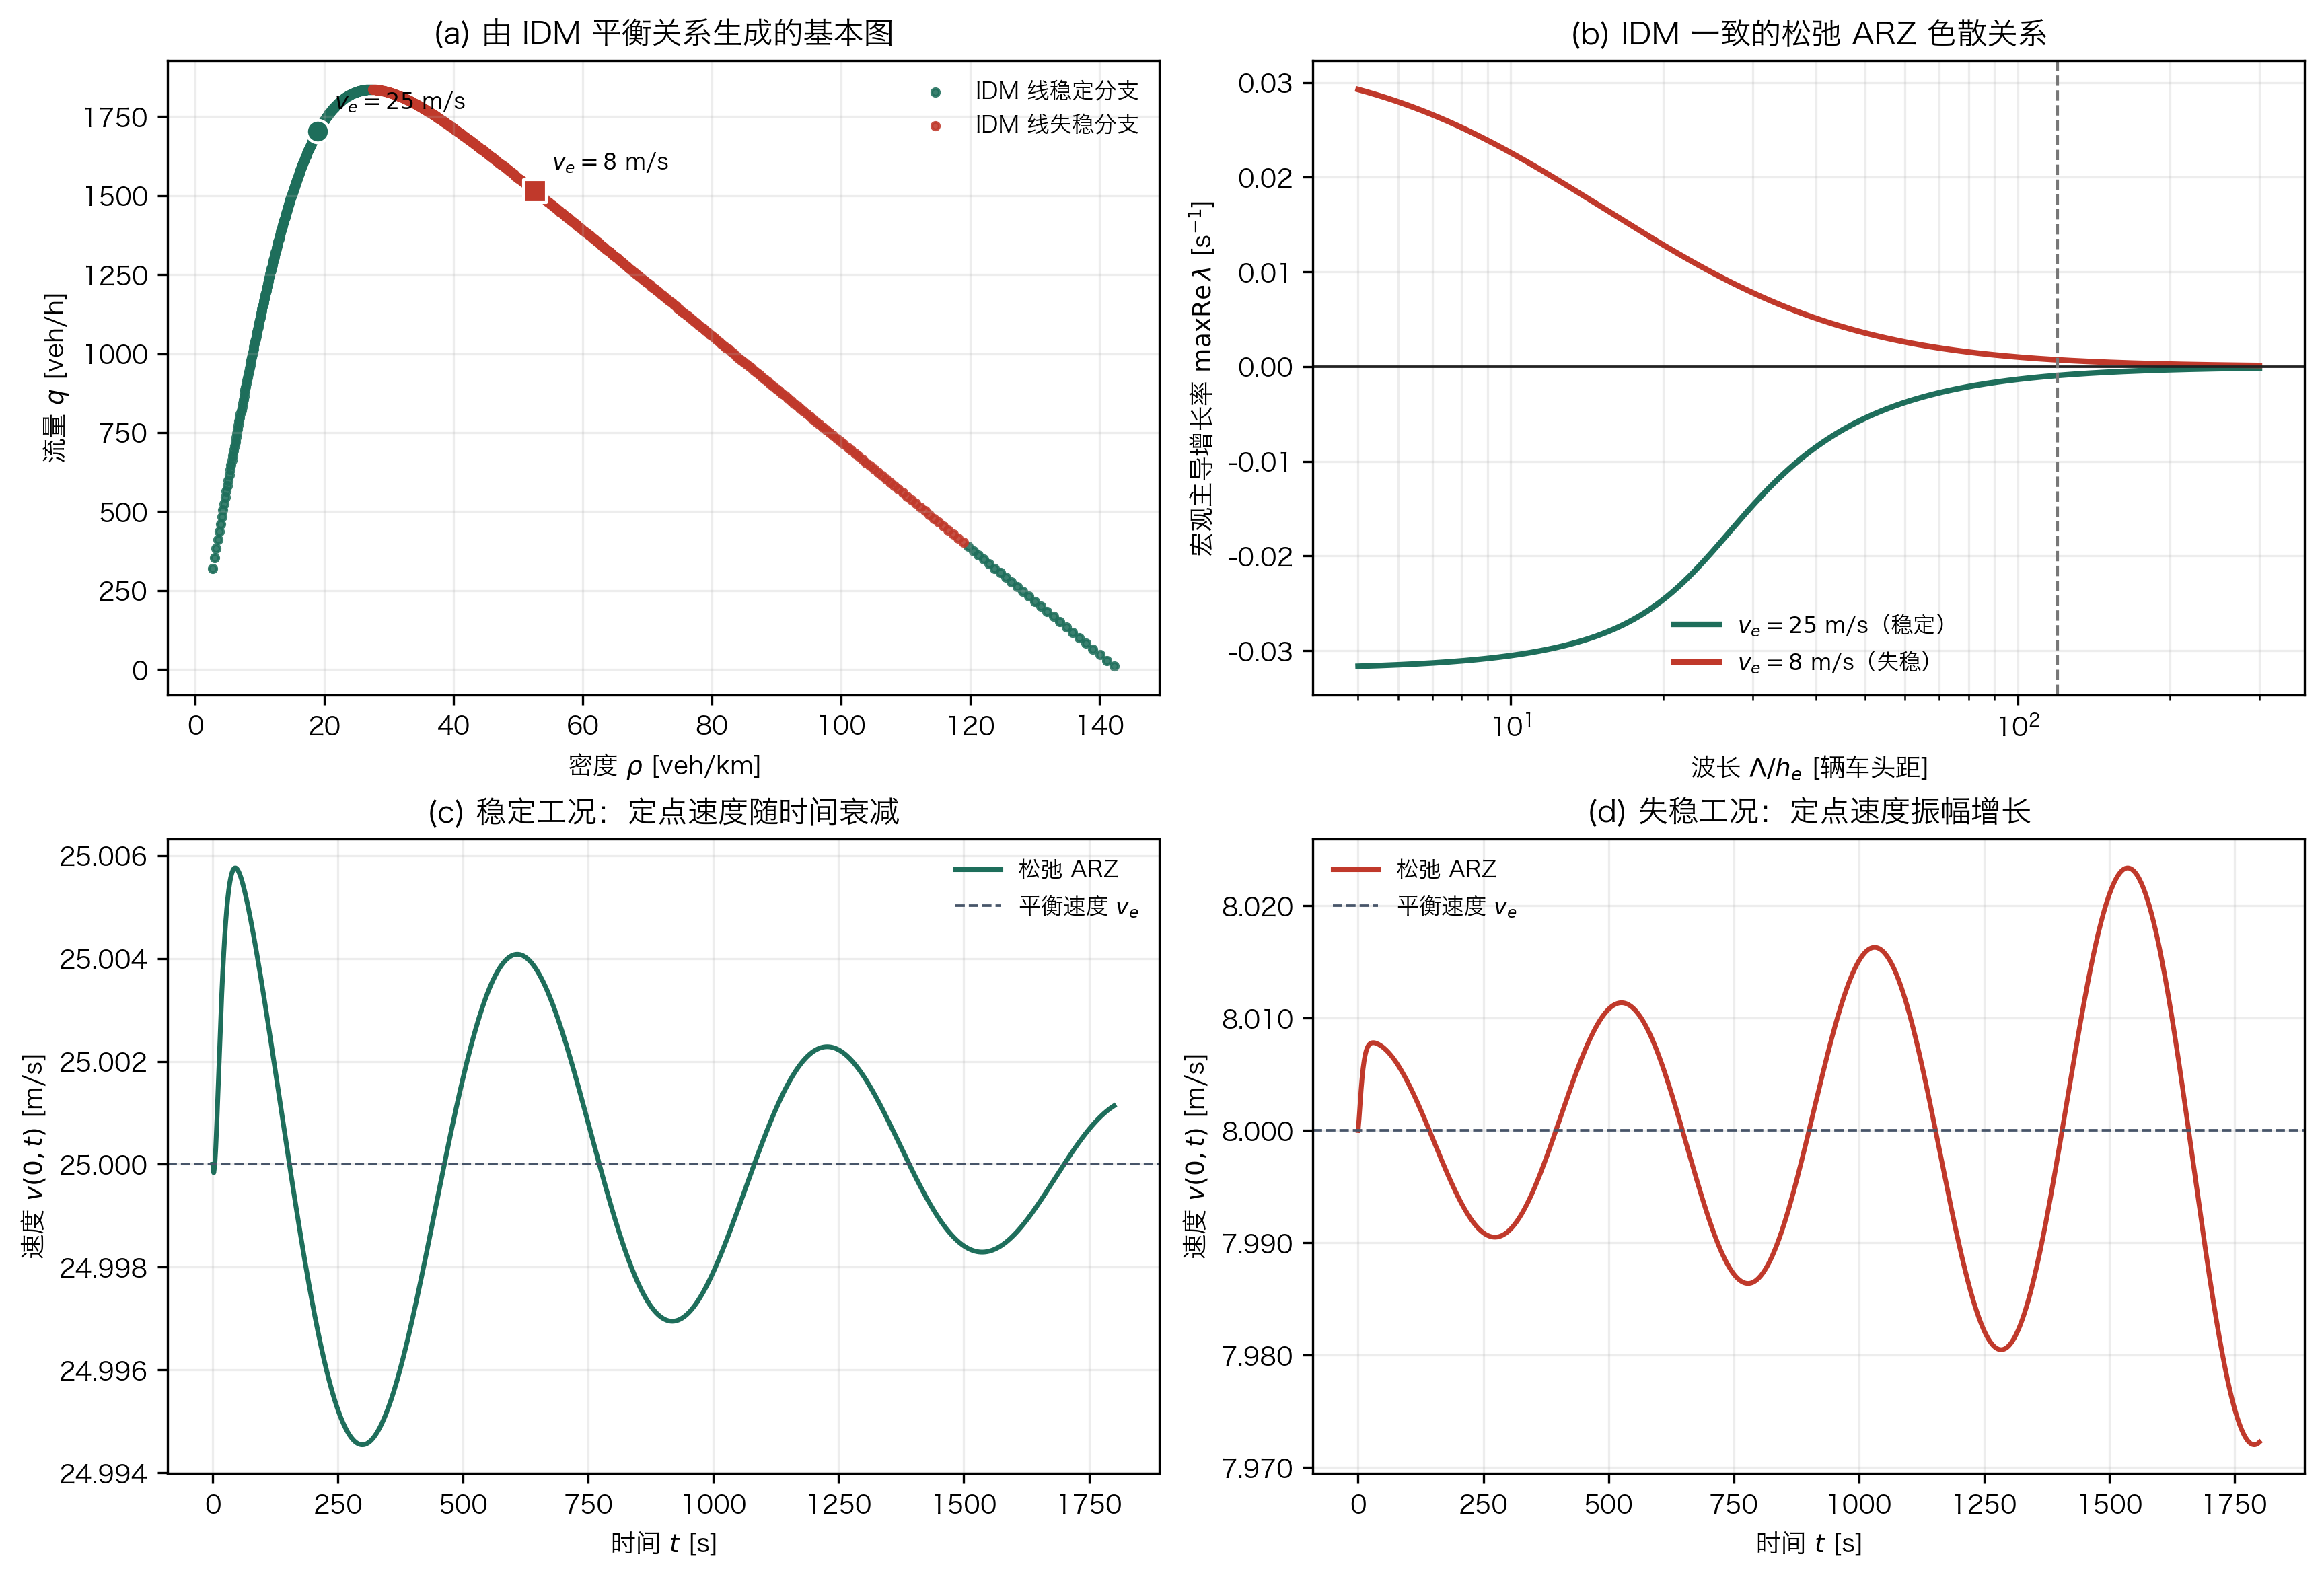
\includegraphics[width=\textwidth]{macroscopic_stability.png}
\caption{A macroscopic stability example for the IDM-consistent ARZ.}
\label{fig:macro-stability}
\figurenote{E13 Hierarchical verification of the macroscopic stability of the IDM-consistent ARZ. Panel (a) first marks stable and unstable operating points on the IDM base diagram to ensure that the macroscopic model has not switched to a different empirical flow-density curve; panel (b) then compares the continuous ARZ dispersion relation with the actual discrete long waves of $N=120,m=1$, with the intersection points indicating the growth rate and phase velocity that should appear in the time domain. In panel (c), the velocity amplitude at the stable fixed point decreases with each cycle, corresponding to the negative real part; in panel (d), the amplitude at the unstable point increases with each cycle, corresponding to the positive real part, and the period matches the imaginary part of the dispersion relation. The consistency—from the basic diagram to the closure of partial derivatives, and then to the consistency of signs in the frequency and time domains—rules out the scenario where “only the equilibrium flow is aligned but the dynamics are opposite.” This figure demonstrates that the ARZ, calibrated using IDM partial derivatives, can reproduce the growth sign and dominant timescale of the microscopic model on a long-wave scale, but does not require the continuous field to replicate the local texture of every discrete vehicle.}
\end{figure}

\begin{tcolorbox}[resultbox,title=\textbf{Quantitative Conclusions of E13}]

On the exact same IDM equilibrium curve, the ARZ long wave at $v_e=25$ m/s is reduced to $18.5\%$ after 1800 s, while the long wave at $v_e=8$ m/s grows to $360.6\%$. The phase velocity under unstable conditions is negative, indicating that the wave propagates upstream; under stable conditions, the phase velocity is positive, indicating that small disturbances propagate downstream with traffic and dissipate. Therefore,




\textbf{The base diagram determines the equilibrium flow rate and kinematic wave velocity, while the dynamic closure determines whether the disturbance grows or decays; both must be consistent with the IDM.}
\end{tcolorbox}

\section{Which macro-level tool should be selected for different problems?}
\sectionstudy{theory}{Which Macro-Level Tool Should Be Chosen for Different Problems?}{treiberkesting2011,daganzo1995,awrascle2000}

\begin{center}
\small
\captionof{table}{Correspondence Between Macro-Level Transportation Problems and Analytical Tools.}
\label{tab:macro-tool-selection}
\begin{tabular}{p{3.0cm}p{4.1cm}p{6.8cm}}
\toprule







Problem




&




 Recommended Models/Tools




&




What They Can and Cannot Answer



\\
\midrule







Queues, Shock Waves, and Congestion Front Speed




& LWR／CTM &




Calculate wave speed and queue length with basic diagrams and conservation laws; the ideal LWR does not provide an intrinsic growth rate.



\\







Smoothing and Dissipation




&




Viscous LWR




&




$D>0$ yields $-Dk^2$ attenuation; a distinction must be made between physical diffusion and numerical diffusion.



\\







Linear Generation of Standing Waves




&




Second-Order Relaxation Models (PW, ARZ, etc.)




&




 Determine the growth rate and dominant wavelength using dispersion relations and sub-characteristic conditions; hyperbolicity and anisotropy must be checked.



\\







Finite-amplitude shock waves and phase transitions




&




 Nonlinear conservation laws, traveling wave/bifurcation analysis




&




Study the coexistence of shock waves, sparse waves, hysteresis, and phases; do not rely solely on linearization at equilibrium points.



\\







Inlet, Outlet, and Fixed Bottleneck& Open-Boundary Spectrum, Convective/Absolute Stability




&




Determine whether the perturbation is carried away or occupies a fixed position; examining only the real $k$ spectrum of the periodic boundary is insufficient.



\\







Model and Controller Calibration




&




 Micro-macro consistency check




&




 Simultaneously align the fundamental diagram, relaxation time, wave velocity, and growth rate; fitting only the flow-density curve is insufficient to ensure correct dynamic stability.



\\
\bottomrule
\end{tabular}
\end{center}
\tabletext{tab:macro-tool-selection}{




Recommended tools and capability limits for six categories of problems: queuing, smoothing, stop-and-go waves, finite-amplitude shock waves, open boundaries, and control calibration. It explains that stability issues must first distinguish between the objects of study: conservative shock waves in LWRs, modal growth in second-order models, and convective/absolute instabilities at open boundaries cannot be assessed using the same criterion.
}

\begin{tcolorbox}[keybox,title=\textbf{Relationship Between This Chapter and Previous Sections}]

Microscopic models tell us




\textbf{which vehicle responses, feedback topologies, or heterogeneous arrangements}




lead to perturbation amplification on a per-vehicle basis; macroscopic models tell us




\textbf{how fast density/velocity waves propagate and how they form shock waves or grow in road space}




. Kinematic shock waves in first-order LWR, linear instability in second-order models, and serial instability in microscopic vehicle fleets are three related but not interchangeable concepts. Only by linking these three can we explain the phenomenon from controller parameters all the way to the patterns of congestion waves on the road.


\end{tcolorbox}

%==================================================================
\sectionwrapup{The non-diffusive small perturbation in LWR is neutral transport, while PW and ARZ have relaxation roots and hydrodynamic roots, respectively; the $k^2$ term of the hydrodynamic root determines long-wave growth. For open channels, a complex wavenumber clamping criterion is also required to distinguish between convection and absolute instability; conclusions cannot be drawn based solely on the real wavenumber spectrum of the ring channel.}

\chapter{Quantitative Link Between Macro- and Micro-Scales: The IDM-Consistent Continuous-Flow Limit}
\label{sec:micro-macro-bridge}
\chapterguide{How to Ensure Macro-Scale Models and IDM Are Truly Comparable Under the Same Operating Conditions}{




This chapter links the two scales via the head-to-head distance–density relationship and the Lagrangian–Eulerian coordinate transformation, then uses the IDM fundamental diagram and dynamic partial derivatives to calibrate macroscopic closure, ensuring that equilibrium flow, wave velocity, and long-wave growth rate are consistent across all levels.
}










The previous chapter introduced the microscopic trailing-wave model and the macroscopic continuous-flow model, respectively; however, “correlation between the two” does not equate to “numerical consistency between the two.” If the macroscopic model uses the Greenshields basic diagram while the microscopic model uses the IDM equilibrium relations, even when both are discussing the same velocity, the equilibrium density, wave velocity, and capacity points will not be the same; furthermore, if the macroscopic relaxation time and pressure function are chosen arbitrarily, there is even less reason for the steady-state boundaries to be consistent. This chapter establishes a computable bridge:




\textbf{The equilibrium layer is generated using the IDM basic diagram, while the dynamic layer is calibrated using IDM long-wave coefficients to achieve macroscopic closure}




. PW is used to demonstrate the simplest symmetric pressure closure, while the final spatiotemporal plot employs ARZ relaxation, which better accounts for traffic anisotropy.










\section{Consistency of the first layer: Basic macro-scale plot generated by IDM}
\sectionstudy{model}{Consistency of the first layer: Basic macro-scale plot generated by IDM}{jin2003,helbing2001,treiberkesting2013}





For a uniform IDM, the net headway is a function of the equilibrium speed:

\begin{equation}
s_e(v)=\frac{s_0+vT}{\sqrt{1-(v/v_0)^\delta}}.
\label{eq:bridge-idm-gap}
\end{equation}

Let the headway be $h_e=s_e+\ell$. Why is the density $1/h_e$? Consider a road segment containing $M$ consecutive headway intervals, with a length of approximately $Mh_e$ and a number of vehicles equal to $M$. Therefore, when the average scale is sufficiently large,

\begin{equation}
\rho_e(v)=\lim_{M\to\infty}\frac{M}{Mh_e(v)}=\frac{1}{h_e(v)},
\qquad
q_e(v)=\rho_e(v)v.
\label{eq:bridge-idm-fundamental}
\end{equation}

Equation ~\eqref{eq:bridge-idm-fundamental} is the IDM basic model in parametric form; no separate assumptions regarding the Greenshields, Underwood, or triangular basic models are required. It guarantees that the micro- and macro-levels have the same $s_e$, $\rho_e$, and $q_e$ for any given $v_e$.




Take the derivative of $v=V(s)$ along the equilibrium curve and use $\rho=1/(s+\ell)=1/h$. Since

\begin{equation}
\frac{\mathrm d\rho}{\mathrm ds}=-\frac{1}{(s+\ell)^2}=-\frac1{h^2},
\qquad
\frac{\mathrm ds}{\mathrm d\rho}=-h^2,
\end{equation}

the chain rule yields

\begin{equation}
V_\rho
=\frac{\mathrm dV}{\mathrm ds}\frac{\mathrm ds}{\mathrm d\rho}
=-h^2V_s,
\qquad
q'(\rho)=V+\rho V_\rho=V-hV_s.
\label{eq:bridge-wave-speed}
\end{equation}

Therefore, as long as the macroscopic base map originates from the same IDM, the LWR kinematic wave velocity $q'(\rho)$ automatically equals the propagation speed of the microscopic long wave in road coordinates. The consistency of the base map resolves




\textbf{phase velocity}




, but the growth rate has not yet been resolved.










\section{Second-level consistency: transforming microscopic long-wave coefficients into macroscopic closed-form expressions}
\sectionstudy{theory}{Second-Order Consistency: Transforming Microscopic Long-Wave Coefficients into Macroscopic Closure}{jin2003,helbing2001,treiberkesting2013}










Let the partial derivative of the reference-following model after linearization be $f_s,f_v,f_{v_l}$, and define

\begin{equation}
\mu=f_v+f_{v_l}<0.
\label{eq:bridge-mu}
\end{equation}

In Chapter ~\ref{sec:appx}~, the long-wave expansion of the vehicle ID coordinates was derived as

\begin{equation}
\lambda_{\rm mic}(k)
=-\mathrm{i}c_1k-c_2k^2+O(k^3),
\qquad
c_1=-\frac{f_s}{\mu},
\qquad
c_2=\frac{c_1^2-\frac12f_s-f_{v_l}c_1}{\mu}.
\label{eq:bridge-micro-longwave}
\end{equation}

Here, $n$ is




\textbf{Lagrangian coordinates}




: The observer moves along with a specific vehicle number; the $x$ for the macroscopic model is




\textbf{Euler coordinates}: The observer stands at a fixed position on the road. The transformation between the two can be derived directly from the uniform trajectory. Since the vehicle numbers in this book increase upstream, the equilibrium trajectory is

\begin{equation}
x_n^0(t)=V_et-nh_e,
\qquad
n=\frac{V_et-x}{h_e}.
\label{eq:bridge-label-position}
\end{equation}

If $g(n,t)=G(x,t)$ represents the same slowly varying perturbation, then the chain rule yields

\begin{equation}
\left.\frac{\partial g}{\partial t}\right|_n
=\left.\frac{\partial G}{\partial t}\right|_x+V_eG_x,
\qquad
g_n=-h_eG_x,
\qquad
g_{nn}=h_e^2G_{xx}.
\label{eq:bridge-derivative-transform}
\end{equation}

The long-wave equation in the vehicle coordinate system is equivalent to Equation ~\eqref{eq:bridge-micro-longwave}:

\begin{equation}
g_t+c_1g_n=c_2g_{nn}.
\label{eq:bridge-lagrangian-pde}
\end{equation}

Substituting Equation ~\eqref{eq:bridge-derivative-transform} term by term:

\begin{align}
G_t+V_eG_x+c_1(-h_eG_x)&=c_2h_e^2G_{xx},\\
G_t+\underbrace{(V_e-h_ec_1)}_{q'(\rho_e)}G_x
&=\underbrace{c_2h_e^2}_{D_{\rm IDM}}G_{xx}.
\label{eq:bridge-eulerian-pde}
\end{align}

For the Euler-Fourier mode $G\propto e^{\lambda t+\mathrm{i}Kx}$, we obtain

\begin{equation}
\lambda_{\rm mic}^{(x)}(K)
=-\mathrm{i}K\underbrace{(V_e-h_ec_1)}_{q'(\rho_e)}
-\underbrace{c_2h_e^2}_{D_{\rm IDM}}K^2
+O(K^3h_e^3),
\qquad K=\frac{k}{h_e}.
\label{eq:bridge-eulerian-longwave}
\end{equation}

This step can also be verified using a phase check: Substituting $n=(V_et-x)/h_e$ into $e^{\lambda t+\mathrm{i}kn}$ simultaneously produces the vehicle translation term $V_e$ and the number propagation term $-h_ec_1$; the difference between the two represents the wave velocity in road coordinates. The vehicle itself can travel downstream, but when $V_e-h_ec_1<0$ occurs, the congestion wave still propagates upstream.




In this context,

\begin{equation}
D_{\rm IDM}=c_2h_e^2
\label{eq:bridge-idm-diffusion}
\end{equation}

represents the equivalent diffusion of the microscopic IDM at the road scale: when $c_2>0$, $D_{\rm IDM}>0$ occurs, causing the disturbance to decay; when $c_2<0$, negative diffusion occurs, leading to long-wave growth.This isn’t simply a matter of “replacing the vehicle number with ‘m’” out of thin air: the first derivative yields a $h_e$, and the second derivative yields a $h_e^2$, so the unit of $D_{\rm IDM}$ is precisely m$^2$/s.










\section{Third-level consistency: Separately calibrate the dynamic closure of PW and ARZ}
\sectionstudy{theory}{Third-level consistency: Separately calibrate the dynamic closure of PW and ARZ}{payne1971,daganzo1995,jin2003}










First, match the fast recovery root of $k=0$. The microscopic fast root is $\mu=f_v+f_{v_l}<0$, and the fast roots for both PW and ARZ are $-1/\tau$; therefore,

\begin{equation}
\boxed{\tau=-\frac1\mu.}
\label{eq:bridge-tau-calibration}
\end{equation}




The long-wave root of the PW-type macroscopic model is given by ~\eqref{eq:pw-hydro-root}. Requiring $D_{\rm eff}=D_{\rm IDM}$ yields

\begin{equation}
\boxed{
c_0^2=(\rho_eV_\rho)^2+\frac{D_{\rm IDM}}{\tau}
}
\label{eq:bridge-pw-calibration}
\end{equation}

Thus, PW simultaneously matches:







\begin{enumerate}[leftmargin=1.5em,itemsep=3pt]
\item




 The fast-recovery root of $k=0$: $-1/\tau=\mu$;







\item




 First-order phase term: $V+\rho V_\rho=V-hc_1$;







\item




Second-order growth/decay term: $D_{\rm eff}=D_{\rm IDM}=c_2h^2$.


\end{enumerate}





For ARZ, let

\begin{equation}
A=\rho_eV_\rho=-h_ec_1<0,
\qquad
B=\rho_ep'(\rho_e)>0.
\end{equation}

be defined by the expressions ~\eqref{eq:arz-effective-diffusion} and $D_{\rm ARZ}=-\tau A(A+B)$. Setting it equal to $D_{\rm IDM}$ allows us to directly solve for the required local pressure gradient:

\begin{equation}
\boxed{
B=-\frac{D_{\rm IDM}}{\tau A}-A,
\qquad
p'(\rho_e)=\frac{B}{\rho_e}.
}
\label{eq:bridge-arz-calibration}
\end{equation}

Under stable conditions $D_{\rm IDM}>0$, equation \eqref{eq:bridge-arz-calibration} yields $B>-A$, so the LWR wave velocity $V+A$ lies within the $[V-B,V]$ of ARZ; Under unstable conditions $D_{\rm IDM}<0$, $B<-A$, the sub-characteristic condition is precisely violated. ARZ therefore not only replicates the sign of the growth rate but also replicates the physical reason for “whether the sub-characteristic condition is satisfied.”










\begin{tcolorbox}[notebox,title=\textbf{Why is replacing only the base diagram insufficient?}]

The base diagram only fixes $V(\rho)$ and $q'(\rho)$; it does not include dynamic information such as how quickly the driver recovers or how strong the relative speed feedback is. Two models can have exactly the same traffic-density curve, yet one may be stable while the other is unstable. Equations ~\eqref{eq:bridge-tau-calibration}~ and ~\eqref{eq:bridge-arz-calibration}~ incorporate the dynamic partial derivatives of IDM into the macro model, which is what causes the stability symbol and the long-wave growth rate to converge. This book retains the PW parameters for analytical cross-checking, but the main figures in E13/E14 use ARZ because it satisfies both IDM long-wave matching and traffic anisotropy.


\end{tcolorbox}

\section{Closing Parameters for Two Reference Operating Conditions}
\sectionstudy{model}{Closing Parameters for Two Reference Operating Conditions}{jin2003,helbing2001,treiberkesting2013}










Substituting the reference IDM parameters from Chapter ~\ref{sec:num}~ yields:







\begin{center}
\captionof{table}{PW/ARZ closure parameters consistent with IDM.}
\label{tab:bridge-closure-parameters}
\resizebox{\textwidth}{!}{%
\begin{tabular}{lrrrrrr}
\toprule







Operating Conditions




& $v_e$ & $\rho_e$ & $\tau$ & $D_{\rm IDM}$ & $c_0$（PW） & $B=\rho p'$（ARZ） \\
& [m/s] & [veh/km] & [s] & [m$^2$/s] & [m/s] & [m/s] \\
\midrule







Stable




& 25 & 18.933 & 9.742 & $+951.43$ & 17.700 & 21.335 \\







Instability




& 8 & 52.567 & 4.646 & $-97.46$ & 11.699 & 10.893 \\
\bottomrule
\end{tabular}
}
\end{center}
\tabletext{tab:bridge-closure-parameters}{




The stable and unstable operating points are uniquely determined by the relaxation time, equivalent diffusion, PW sound speed, and ARZ pressure gradient derived from the IDM dynamic gradients. The stable rows satisfy the sub-characteristic conditions and exhibit positive diffusion, while the unstable rows exhibit both violations of the sub-characteristic conditions and negative diffusion, indicating that macro-micro consistency here goes beyond mere alignment of the basic diagrams.
}







Under stable operating conditions, $-A=14.684$ m/s applies, while $B=21.335>-A$ holds and the ARZ sub-criterion is satisfied; under unstable operating conditions, $-A=12.563$ m/s applies, while $B=10.893<-A$ holds and the sub-criterion is violated. The values $c_0$ and $B$ in the table were not manually adjusted to achieve “desired results”; rather, they are local closed-loop values determined for each equilibrium point by equations ~\eqref{eq:bridge-pw-calibration} and ~\eqref{eq:bridge-arz-calibration}, respectively.










\section{E14: Micro-Macro Spatiotemporal Diagram Under Identical IDM Conditions}
\sectionstudy{experiment}{E14: Micro-Macro Spatiotemporal Diagrams Under Identical IDM Conditions}{jin2003,helbing2001,treiberkesting2013}







\label{sub:micro-macro-experiment}




Both models use exactly the same $v_e$, $\rho_e$, loop length, and initial perturbation:







\begin{itemize}[leftmargin=1.4em,itemsep=3pt]
\item




 $N=120$, taking the longest non-zero loop mode $m=1$, hence $\Lambda=L=N(s_e+\ell)$;







\item




 The initial velocity perturbation is $0.05\sin(2\pi n/N)$ m/s, and the initial spacing is uniform;







\item




 Simulation time: 1800 s; the IDM is fully nonlinear on the microscopic side, with an RK4 step size of $0.05$ s;







\item




 On the macroscopic side, the linearized relaxation ARZ is advanced exactly using spectral methods, and IDM-consistent closure is applied according to equations ~\eqref{eq:bridge-tau-calibration} and \eqref{eq:bridge-arz-calibration};







\item




 In Figure ~\ref{fig:micro-macro-idm}, the horizontal axis represents time, the vertical axis represents normalized road position $x/L$, and the colors represent velocity perturbations $v-v_e$.


\end{itemize}


$x/L$ is used instead of absolute kilometer values because the two conditions have different equilibrium densities: the loop length for the stable condition is 6.338 km, while for the unstable condition it is 2.283 km. Normalizing the position ensures that both rows display a complete loop without altering the direction of the wave’s slope.










\begin{figure}[!t]
\centering
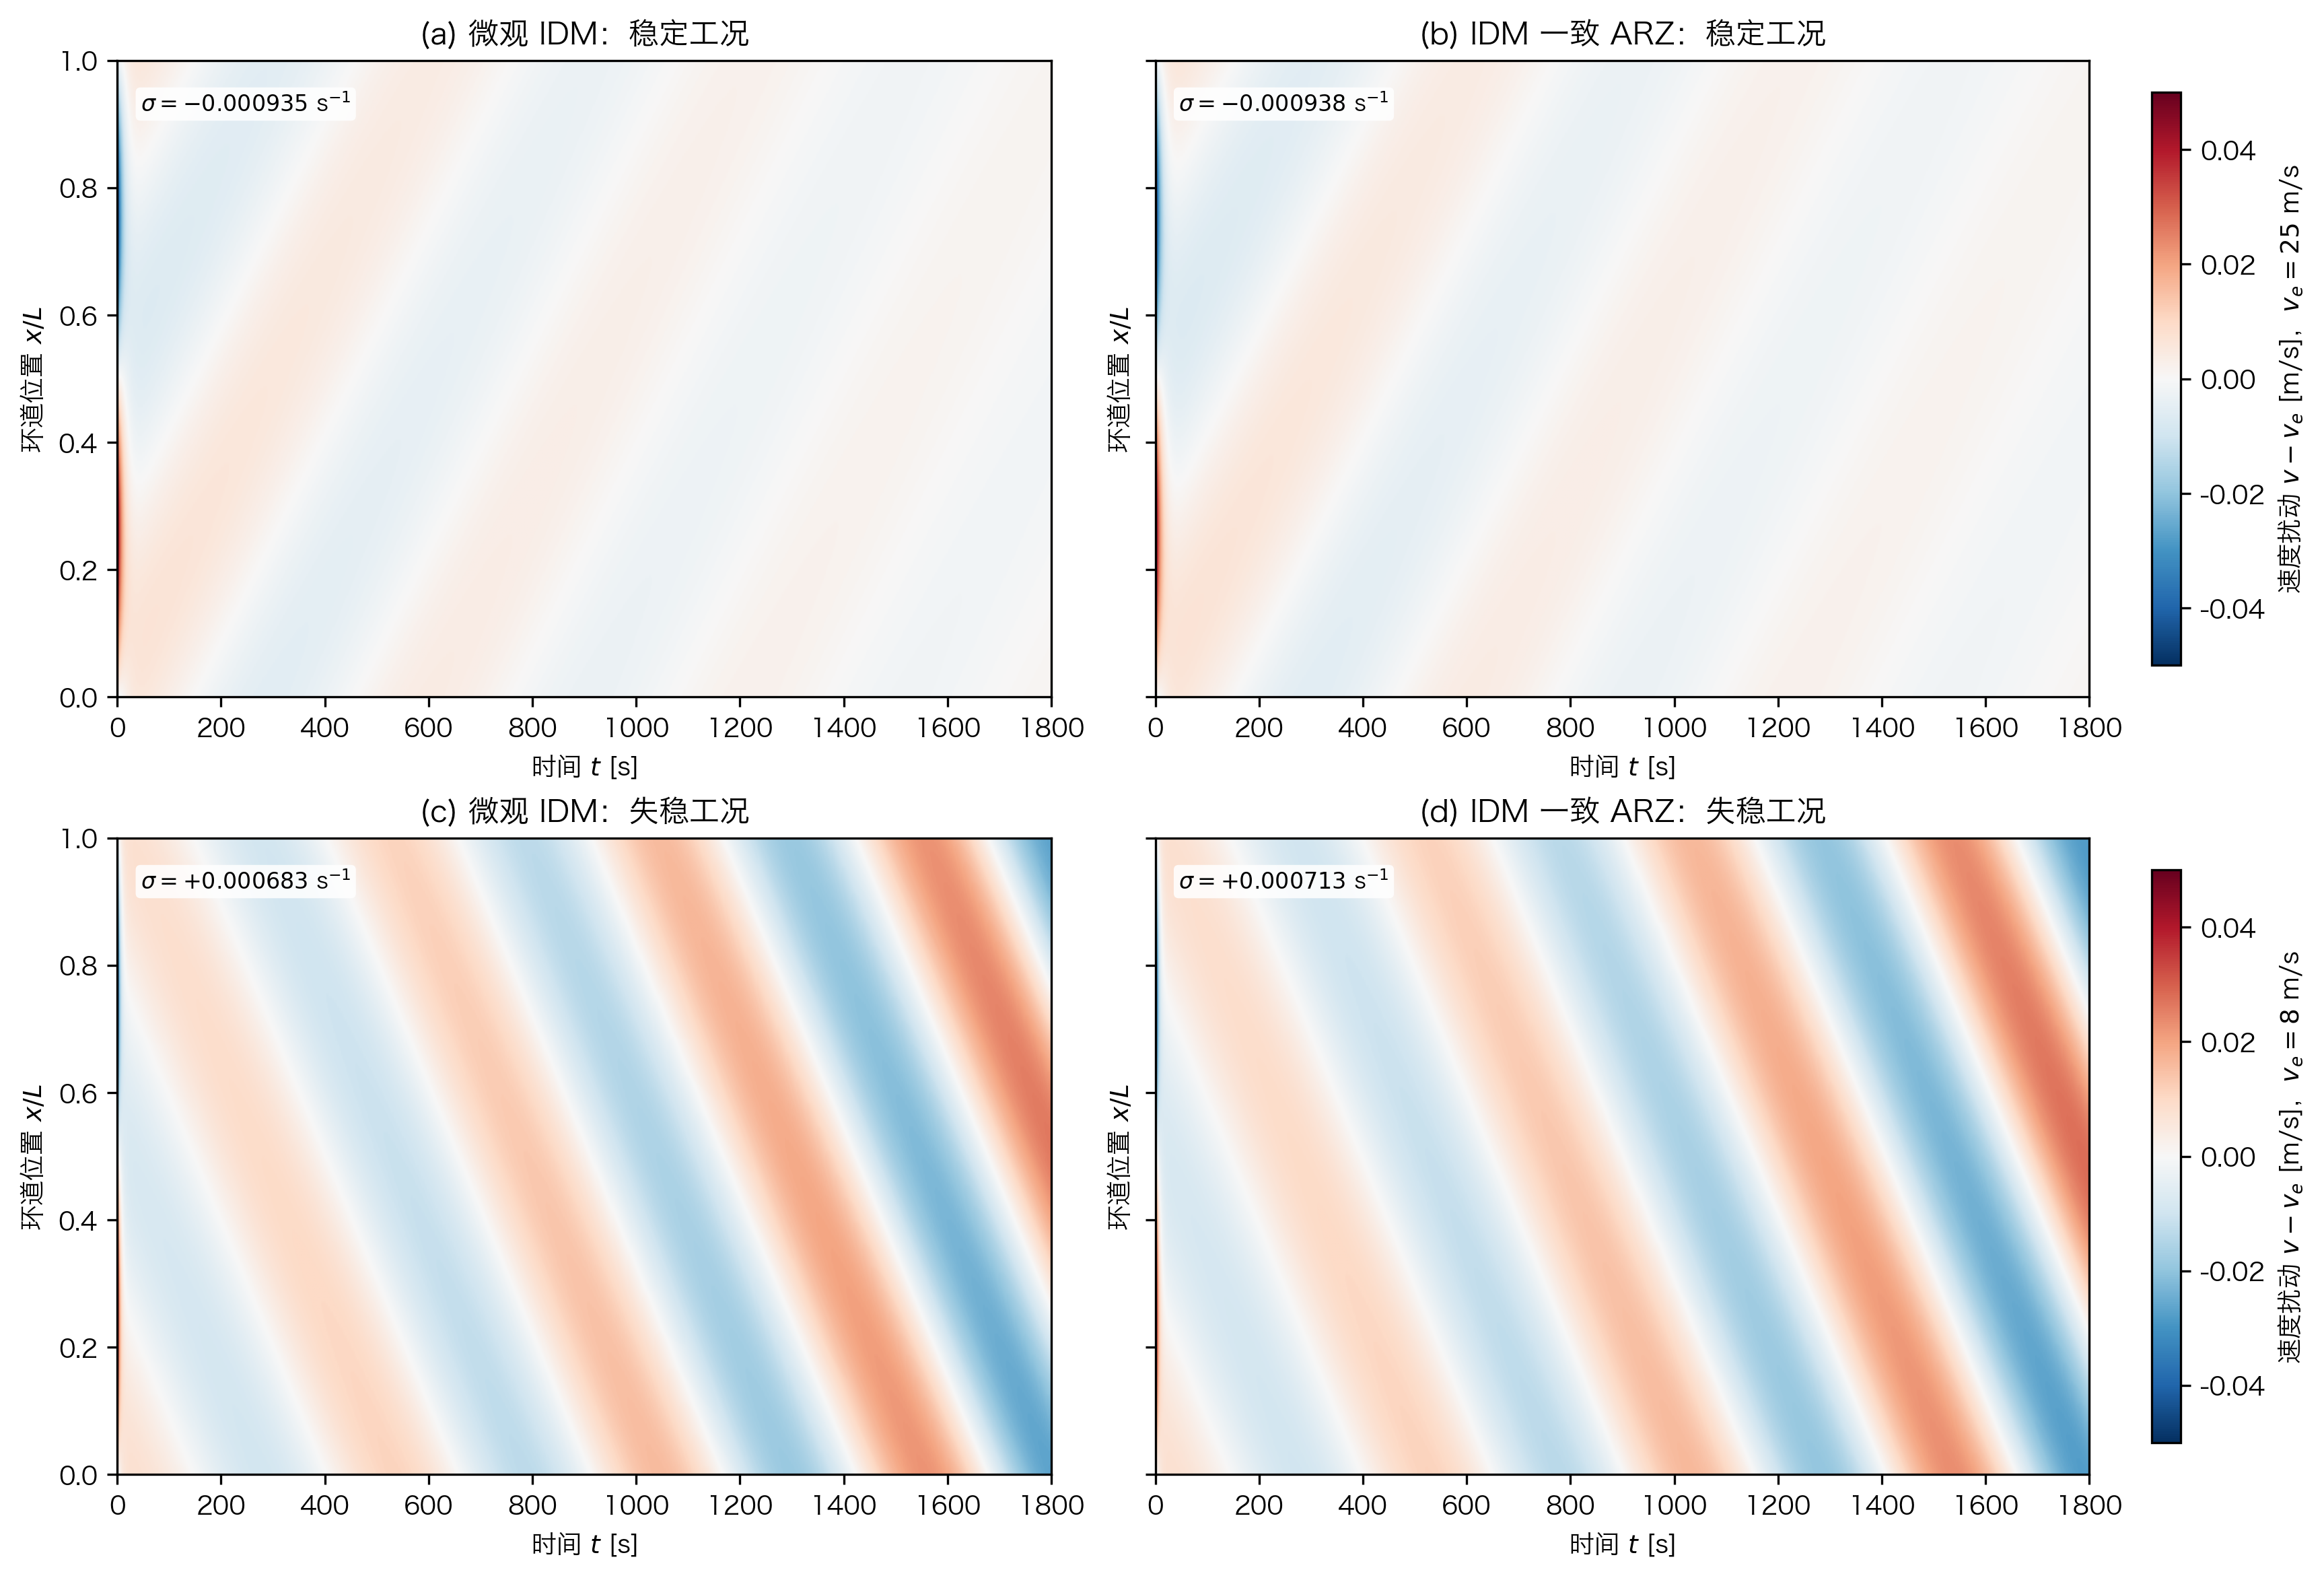
\includegraphics[width=\textwidth]{micro_macro_idm_comparison.png}
\caption{Comparison of macro- and micro-scale velocity-time-space maps between IDM and ARZ.}
\label{fig:micro-macro-idm}
\figurenote{E14 directly compares the micro-scale IDM and macro-scale ARZ velocity-time-space fields in fixed road coordinates. Both columns use the same IDM base map, the same $v_e$, density, loop length, and initial $m=1$ long wave; Each row shares the same color range; the horizontal axis represents time, and the vertical axis represents $x/L$, allowing for a direct comparison of the color band slopes and intensities. In the stable row ($v_e=25$ m/s), the positive and negative perturbation bands of both models fade over time, and their propagation slopes are similar, demonstrating that they provide consistent predictions for the decay rate and phase velocity; In the unstable line $v_e=8$ m/s, the color bands tilt toward the smaller $x$ and gradually intensify, demonstrating that both models predict growing waves propagating upstream. The micro-scale image preserves individual vehicle trajectories and finer textures, while the macro-scale image depicts a smooth, continuous field; these local differences stem from scale representation rather than conflicting stable conclusions. This figure demonstrates that only when the IDM base map, relaxation time, and pressure gradient are simultaneously matched will macro- and micro-scale models yield similar spatiotemporal road evolution under identical conditions.}
\end{figure}

\section{Quantitative Comparison of Growth Rates, Wave Speeds, and Image Similarity}
\sectionstudy{theory}{Quantitative Comparison of Growth Rates, Wave Speeds, and Image Similarity}{jin2003,helbing2001,treiberkesting2013}

\begin{center}
\small
\captionof{table}{Dynamic error of ARZ consistent with IDM and IDM.}
\label{tab:micro-macro-dynamic-errors}
\begin{tabular}{lrrrrr}
\toprule







Operating conditions




&




 Model




& $\operatorname{Re}\lambda$ [s$^{-1}$] &




 Phase velocity [m/s]




&




 Growth rate error




&




 Wave speed error



\\
\midrule







Steady




&




 Micro IDM




& $-0.0009355$ & $+10.293$ & -- & -- \\







Stable




&




 IDM Consistent ARZ




& $-0.0009377$ & $+10.241$ & $0.24\%$ & $0.51\%$ \\
\midrule







Instable




&




 Micro IDM




& $+0.0006827$ & $-4.469$ & -- & -- \\







Instability




&




 IDM consistent ARZ




& $+0.0007126$ & $-4.516$ & $4.37\%$ & $1.05\%$ \\
\bottomrule
\end{tabular}
\end{center}
\tabletext{tab:micro-macro-dynamic-errors}{




Prediction of growth rate and phase velocity for the same long wave by micro IDM and continuous ARZ. The errors at both scales are less than $1\%$ under stable conditions, and they maintain the same sign and propagation direction under instability; the remaining differences arise from discrete vehicles versus the continuous field and from higher-order terms with finite wavenumbers.}





To avoid simply stating that they “look very similar” based on visual inspection alone, we averaged the velocity perturbation field at each time step and divided it by its spatial standard deviation, then calculated the average correlation coefficients between the microscopic and macroscopic fields from 0 to 1500 s:

\begin{equation}
\mathcal S
=\left\langle
\frac{u_{\rm mic}}{\sigma_{\rm mic}}
\frac{u_{\rm mac}}{\sigma_{\rm mac}}
\right\rangle_{x,t}.
\label{eq:bridge-similarity}
\end{equation}

Under steady-state conditions, $\mathcal S=0.9977$ is obtained, and under unstable conditions, $\mathcal S=0.9913$ is obtained. This indicates that not only do the two share the same stability sign, but the propagation directions, tilt angles, and phase positions of the red and blue bands are also highly consistent. After 1,800 s, the theoretical amplitude ratios of the microscopic field to the ARZ are:

\begin{equation}
\begin{array}{c|cc}
&\text{Microscopic IDM}&\text{IDM-consistent ARZ}\\ \hline
v_e=25\ {\rm m/s}&0.186&0.185\\
v_e=8\ {\rm m/s}&3.417&3.606
\end{array}
\label{eq:bridge-amplitude-ratios}
\end{equation}










\begin{tcolorbox}[resultbox,title=\textbf{Key Conclusions of E14}]
\begin{itemize}[leftmargin=1.3em,itemsep=3pt]
\item




After replacing the Greenshields diagram with the IDM basic diagram, the microscopic and macroscopic models first show consistency in density, flow rate, and kinematic wave velocity.







\item




Only after calibrating $\tau$, $p'(\rho_e)$, and $D_{\rm ARZ}$ using the IDM partial derivatives do the two models converge in terms of stability symbols, growth rates, and propagation speeds.







\item




At $v_e=25$ m/s, both color bands fade over time; at $v_e=8$ m/s, both color bands tilt upstream and deepen. Stability/instability no longer depends on the arbitrary selection of different macroscopic parameters.







\end{itemize}
\end{tcolorbox}

\section{How far does this consistency extend?}
\sectionstudy{synthesis}{How far does this consistency extend?}{jin2003,helbing2001,treiberkesting2013}










This chapter verifies that\textbf{Small Disturbances, Long Waves, Uniform Single-Lane}




Limit. The macroscopic model only matches up to $O(K^2)$; dispersion at the finite wavelength ($O(K^3)$), high-wavenumber truncation caused by discrete vehicles, and nonlinear saturation following stop-and-go conditions are still determined by the full IDM. Therefore:







\begin{itemize}[leftmargin=1.4em,itemsep=3pt]
\item




When $m/N\to0$, the growth rate and wave speed errors should continue to decrease;







\item




When perturbations have evolved into standing waves, linear macroscopic closures cannot replace a full microscopic simulation;







\item




Heterogeneous vehicles, lane changes, communication topologies, and reaction delays require additional macroscopic states or nonlocal closures and cannot be captured solely by a single IDM base diagram.







\end{itemize}







This also illustrates that a macroscopic model is not merely “another way of drawing” a microscopic model, but rather an approximation obtained through spatial averaging and scale truncation; consistency must explicitly specify which orders and which observables are matched.




%==================================================================







\sectionwrapup{The IDM basic diagram ensures consistency between macroscopic and microscopic equilibrium densities, flow rates, and kinematic wave speeds; the Lagrangian-to-Eulerian coordinate transformation further establishes a correspondence between vehicle number waves, road wavelengths, and long-wave diffusion coefficients. Only by calibrating $\tau$ and $p'(\rho)$ using IDM dynamic gradients can the growth rates at the macro- and micro-levels be quantitatively matched.}

\chapter{Evidence of stability in real-world trajectories: NGSIM}
\label{sec:ngsim}
\chapterguide{How to Effectively Utilize Real-World Trajectories for Stability Modeling and Decision-Making}{




This chapter first uses D01 to extract propagation evidence from position-time trajectories, a continuous eight-vehicle convoy, and 78 natural segments. It then uses D02 to comprehensively cover the three major phases—“stability convoy calibration, simulation validation, and stability optimization and evaluation”—while clearly distinguishing which conclusions stem from the data and which arise from model counterfactuals.
}










The stability conclusions presented earlier are based on well-defined models and steady states. Real-world roads, however, involve lane changes, ramps, driver variations, measurement errors, and constantly changing boundary inputs; therefore, a segment of measured spatiotemporal data showing alternating red and blue patterns cannot be directly labeled as “linear instability.” Analysis of real-world data is better suited to answering four progressively deeper questions:







\begin{enumerate}[leftmargin=1.6em,itemsep=3pt]
\item




 Can coherent speed perturbations be identified among consecutive vehicles in the same lane?







\item




 Does the amplitude of the following vehicle’s fluctuations increase or decrease relative to the leading vehicle, and what is the response lag?







\item




 Compared to fitting only a single following vehicle, does incorporating information from the entire train of vehicles allow the model to better reproduce traffic flow during the holdout period?







\item




 Can the stability spectrum of the calibrated model be transformed into control parameters, and then evaluated separately using independent simulations and holdout data?







\end{enumerate}







D01 addresses the first two items; D02 addresses the last two. Together, they form a complete application demonstration, but we do not claim that a single three-minute sample is sufficient for universal calibration of the IDM or road validation of the controller.










\section{Data Sources, Observation Intervals, and Fields}
\sectionstudy{data}{Data Sources, Observation Intervals, and Fields}{ngsim2016,thiemann2008,krajewski2018}





NGSIM was collected by the U.S. Federal Highway Administration. The US-101 data uses synchronized video to reconstruct vehicle trajectories. The official open data provides one record per $0.1$, and it is recommended to cite the dataset using the DOI \cite{ngsim2016}. D01 reads a $179.5$ segment from the official data interface for southbound Lane 2 of US-101, with the query range being

\[
1118846979700\le \texttt{global\_time}\le1118847159700.
\]

. It returns 39,187 rows and 119 vehicles; for this segment,




\texttt{v\_class}




 are all 2, indicating passenger vehicles. The original longitudinal position, speed, acceleration, and headway are in feet; after entering the analysis, they are uniformly multiplied by $0.3048$ to convert to SI units.










\begin{center}
\small
\captionof{table}{NGSIM fields used by D01 and preprocessing.}
\label{tab:ngsim-fields}
\begin{tabular}{p{3.2cm}p{4.8cm}p{5.4cm}}
\toprule
\textbf{Fields} & \textbf{Purpose of This Chapter} & \textbf{Processing} \\
\midrule
\texttt{vehicle\_id}, \texttt{global\_time} &




 Unique Trajectories and Common Timeline




&




Check if Adjacent Frames Differ by 100 ms



\\
\texttt{local\_y}, \texttt{v\_vel} &




Position-Time-Velocity Colored Trajectories




&




 Convert ft and ft/s to m and m/s, respectively



\\
\texttt{preceding}, \texttt{lane\_id} &




 Reconstruct the chain of vehicles in the same lane




&




 A segment is considered the same only if the ID of the leading vehicle remains unchanged



\\
\texttt{space\_headway}, \texttt{time\_headway} &




 Description of Spacing and Time Interval& Remove boundary records where the preceding vehicle ID is 0



\\
\texttt{v\_acc} &




Acceleration Diagnosis




&




For reference only; do not use raw differential values directly to calibrate the model



\\
\bottomrule
\end{tabular}
\end{center}
\tabletext{tab:ngsim-fields}{




Fields used from the official trajectory records to reconstruct the fleet, generate position-time plots, and calculate propagation gains. The table also lists unit conversions and continuity checks, demonstrating that the evidence for D01’s stability does not rely directly on the noisier raw acceleration data.
}

\begin{tcolorbox}[notebox,title=\textbf{Why This Chapter Does Not Directly Fit Raw Acceleration Data}]

Minor errors in position reconstruction are significantly amplified after two time differences, and the switching of the leading vehicle near lane changes causes discontinuities. D01 therefore treats velocity as a subjective measurement and explicitly documents the smoothing window. If IDM is calibrated subsequently, acceleration residuals can only be used in conjunction with trajectory, distance, propagation gain, and set-aside errors; they cannot serve as the sole objective.







\end{tcolorbox}

\section{D01’s Reproducible Processing Workflow}
\sectionstudy{data}{D01’s Reproducible Processing Workflow}{ngsim2016,thiemann2008,krajewski2018}










The data pipeline executes in the following fixed order:







\begin{enumerate}[leftmargin=1.6em,itemsep=3pt]
\item




 Read the specified location, lane, time, and fields from the official API, and save the query criteria and access date;







\item




 Sort by




\texttt{global\_time, vehicle\_id}




, validate the fields, and perform unit conversions;







\item




 Search for the longest




\texttt{preceding}




 chain in the common snapshot at approximately the 100th second, and select 8 vehicles with continuous observations of at least 20 seconds;


\item For all follow-up segments where the leading vehicle’s number remains unchanged and the sequence is continuous for at least 201 frames, apply a 21-frame third-order Savitzky–Golay filter \cite{savitzky1964};







\item




 Remove the linear trend from each speed curve and exclude near-constant segments where the standard deviation of the lead vehicle is less than $0.25$ m/s;







\item




 Calculate the amplitude gain and maximum correlation lag for each vehicle, and use self-sampling with a fixed random seed 20,000 times to obtain the uncertainty interval.







\end{enumerate}










If the smoothed and detrended speeds of the lead vehicle and the following vehicle are $\widetilde v_l(t)$ and $\widetilde v_f(t)$, respectively, the empirical gain defined in this chapter is

\begin{equation}
\Gamma_{f\leftarrow l}
=\frac{\operatorname{std}(\widetilde v_f)}
       {\operatorname{std}(\widetilde v_l)},
\qquad
\tau^*=\arg\max_{0\le\tau\le5\,\mathrm s}
\operatorname{corr}\!\left[\widetilde v_l(t),\widetilde v_f(t+\tau)\right].
\label{eq:ngsim-gain}
\end{equation}

$\Gamma>1$ indicates that the following vehicle’s speed fluctuates significantly within this natural segment, while $\Gamma<1$ indicates that it fluctuates less. It is related to $|G(\mathrm i\omega)|$ from the steady-state sinusoidal experiment, but is not the same quantity: Equation \eqref{eq:ngsim-gain} combines multiple frequencies present in the segment and does not control all external inputs.










\begin{tcolorbox}[experimentbox,title=\textbf{D01 Pseudocode corresponds one-to-one with the actual output}]
\begin{verbatim}
download official slice -> validate schema -> convert ft to m
for each continuous leader-follower episode >= 20 s:
    smooth leader and follower speed with the declared window
    remove each linear trend
    if std(leader) >= 0.25 m/s:
        gain = std(follower) / std(leader)
        lag  = argmax cross_correlation over 0 ... 5 s
bootstrap the episode table -> confidence intervals
save derived CSV + JSON metrics + four-panel figure
\end{verbatim}
\end{tcolorbox}

\section{Consecutive eight-car convoy: The perturbation is not a uniform single sine wave}
\sectionstudy{theory}{Consecutive eight-car convoy: The perturbation is not a uniform single sine wave}{ngsim2016,thiemann2008,krajewski2018}





The automatically selected chain, in order from the lead vehicle to the trailing vehicles, is

\[
395\rightarrow399\rightarrow405\rightarrow411\rightarrow418\rightarrow426\rightarrow431\rightarrow440,
\]

observed simultaneously for 20.0 s. Figure ~\ref{fig:ngsim-d01}(b) shows a noticeable lag between the speed peaks and troughs of different vehicles; the detrended standard deviation in Figure ~\ref{fig:ngsim-d01}(c) does not vary monotonically for each vehicle, but rather decreases for the middle vehicles and then increases again for the upstream vehicles 431 and 440. This is precisely the difference between real-world data and a single Fourier mode: multiple perturbations, heterogeneous parameters, and boundary inputs coexist, so the entire propagation process cannot be summarized using just two values—those of the last and first vehicles.










\section{Statistical Results for 78 Natural Following Segments}
\sectionstudy{data}{Statistical Results for 78 Natural Following Segments}{ngsim2016,thiemann2008,krajewski2018}










After filtering, 78 continuous segments were obtained. The median headway of the sample was 1.77 s, with a quartile range of 1.44–2.18 s; the median response lag was 1.85 s, and the median maximum correlation coefficient was 0.794. The results for empirical gain are

\begin{equation}
\operatorname{median}(\Gamma)=1.033,\qquad
\operatorname{IQR}(\Gamma)=[0.892,1.189],\qquad
\Pr_{\rm sample}(\Gamma>1)=55.1\%.
\label{eq:ngsim-results}
\end{equation}

However, the median 95%




\%




interval obtained from segment-level bootstrap sampling is $[0.954,1.077]$, and the 95%




\%




 interval is $[44.9\%,65.4\%]$; both span the neutral reference value. Therefore, the correct conclusion is not that “US–101 has been proven to be line-unstable,” but rather:




\textbf{This segment exhibits both amplification and attenuation events, with a median empirical gain close to 1; the current sample size is insufficient to rule out neutral propagation at the population level.}

\begin{figure}[htbp]
\centering
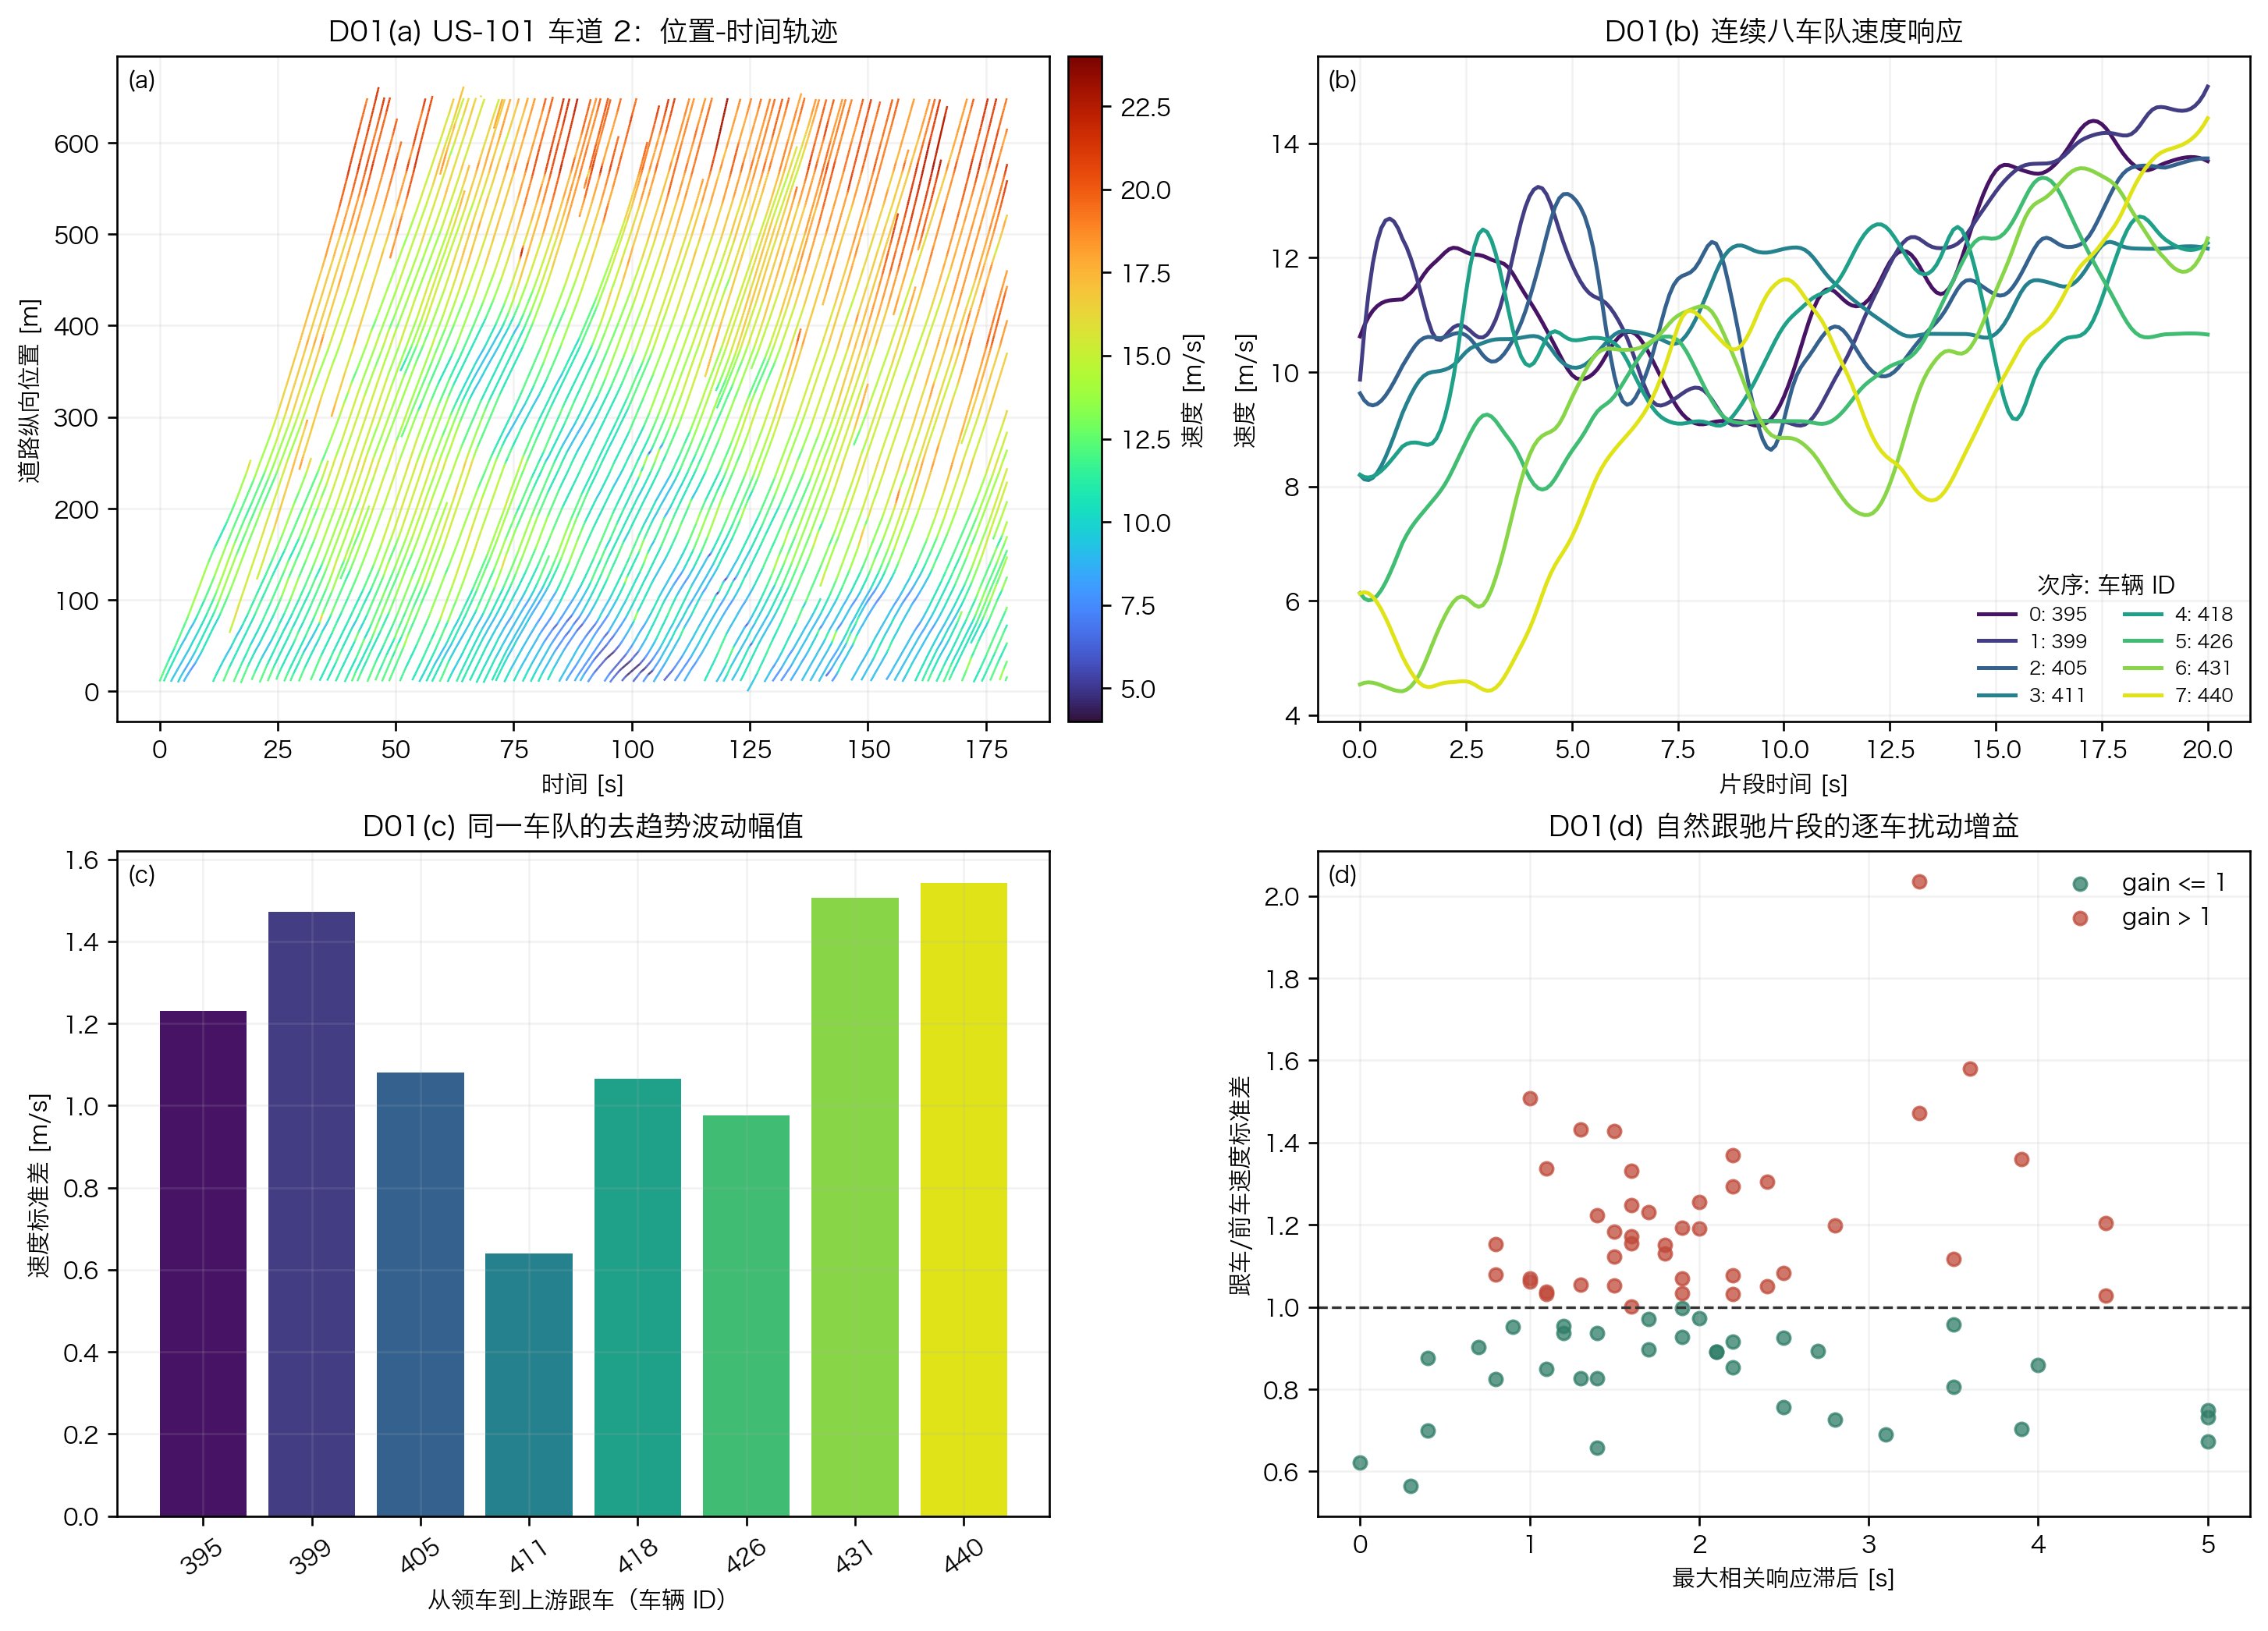
\includegraphics[width=\textwidth]{ngsim_us101_d01.png}
\caption{Stability Diagnosis of Real-World Trajectories from NGSIM US--101.}
\label{fig:ngsim-d01}
\figurenote{D01 Complete processing chain from the raw NGSIM US--101 trajectory to empirical evidence of stability. Panel (a) displays the vehicle trajectory and speed (color-coded) for Lane 2 on a real-time location-time plot, first confirming the presence of propagating speed waves during the selected time period; Panel (b) displays an automatically identified sequence of eight consecutive vehicle convoys; the time lag in the appearance of peaks and troughs along the convoy order indicates causal propagation between vehicles rather than simultaneous external inputs. Panel (c) compares the trend-adjusted standard deviations of individual vehicle speeds, showing that perturbations do not increase or decrease monotonically but instead amplify again after locally attenuating among heterogeneous vehicles; this explains why comparing only the lead and trailing vehicles would overlook intermediate structures. Panel (d) summarizes the empirical gains and lags for 78 natural following segments; the red dots represent only the segment $\Gamma>1$, with a median close to 1 and a confidence interval spanning the neutral value. This figure demonstrates that real-world traffic contains both amplification and attenuation events, supporting the use of stability as a statistical calibration objective; however, a single three-minute sample is insufficient to claim that the entire US-101 route is unstable. Furthermore, the red dots do not serve as collision risk labels.}
\end{figure}

\section{D02 Overall Design: From Real-World Fleets to Evaluable Stability Applications}
\sectionstudy{data}{D02 Overall Design: From Real-World Fleets to Evaluable Stability Applications}{kesting2008,ossen2009,punzo2012}


\label{sub:ngsim-d02}




D02: The eight teams automatically selected using D01

\[
395\rightarrow399\rightarrow405\rightarrow411\rightarrow418
\rightarrow426\rightarrow431\rightarrow440
\]

Complete the three tasks. $0$--$12$ are used for calibration, while $12$--$20$ are left entirely unused; all speeds and spatial headway

are first processed using the same 21-frame third-order filter as in D01. Subtract a uniform train length of $4.8$ m from the spatial headway to obtain the net headway.

To reduce the number of unidentifiable parameters in this short segment, fix $v_0=33.3$ m/s, $\delta=4$, and the train length,

and estimate only $\theta=(T,s_0,a,b)$.










\begin{enumerate}[leftmargin=1.6em,itemsep=3pt]
\item \textbf{Stability Calibration:}




Compare “fitting only the first following vehicle 399” with “simultaneously fitting all seven following vehicles and the perturbation amplitude for each vehicle”;







\item \textbf{Simulation Validation:}




Freeze the parameters, restart from the measured state at the time of separation, use only the separation speed of the lead vehicle 395 as the external input, and simulate the remaining seven vehicles using recursion;







\item \textbf{Optimization and Evaluation:}




Use the loop diagram of the calibrated model to select the minimum lead-vehicle acceleration feedforward gain, then check the model loop diagram and the actual clearance segment separately.







\end{enumerate}







This separation is crucial: Calibration, validation, and optimization rely on different types of information; parameters must not be adjusted retroactively after reviewing the clearance results.





\subsection{Part 1: Why Stability Calibration Is Not the Same as Simply Adding an RMSE}










The traditional single-vehicle objective uses only vehicle 399:

\begin{equation}
J_{\rm one}(\theta)
=\frac{{\rm RMSE}(v_{399}^{\rm sim},v_{399}^{\rm obs})}{1\ {\rm m/s}}
+\frac{{\rm RMSE}(s_{399}^{\rm sim},s_{399}^{\rm obs})}{5\ {\rm m}}.
\label{eq:ngsim-single-objective}
\end{equation}

The stability fleet objective, however, integrates data from all seven following vehicles simultaneously. Let

$A_j={\rm std}\{\operatorname{detrend}[v_j(t)]\}$ represent the speed amplitude for each vehicle in the training segment, and define

\begin{equation}
J_{\rm platoon}(\theta)
=\frac{{\rm RMSE}(\bm v^{\rm sim},\bm v^{\rm obs})}{1\ {\rm m/s}}
+\frac{{\rm RMSE}(\bm s^{\rm sim},\bm s^{\rm obs})}{5\ {\rm m}}
+1.25\,{\rm RMSE}\!\left(\log\bm A^{\rm sim},\log\bm A^{\rm obs}\right).
\label{eq:ngsim-platoon-objective}
\end{equation}

The third term is not simply a matter of “using a few more cars”: it requires the model to preserve the spatial shape of perturbations along the vehicle order, penalizing parameters that fit a local trajectory well

but amplify upstream fluctuations in a completely incorrect manner. Both objectives are solved using the same parameter bounds and random seeds.










\begin{center}
\small
\captionof{table}{D02: IDM parameters obtained from calibrating the two objectives.}
\label{tab:d02-calibrated-parameters}
\begin{tabular}{p{3.7cm}rrrr}
\toprule
\textbf{Calibration Method} & $T$ [s] & $s_0$ [m] & $a$ [m/s$^2$] & $b$ [m/s$^2$]\\
\midrule







Single Car 399




& 0.4458 & 6.000 & 2.257 & 4.500\\







Stability Fleet




& 0.9474 & 6.000 & 1.550 & 0.500\\
\bottomrule
\end{tabular}
\end{center}
\tabletext{tab:d02-calibrated-parameters}{




Two sets of IDM parameters obtained from the single-vehicle target and the stability fleet target. The two sets differ significantly, and parameters in both sets approach the boundaries, indicating that short-term single-vehicle trajectories cannot uniquely identify the propagation characteristics of disturbances in the traffic flow layer. The parameter results must be interpreted in conjunction with training and holdout errors.
}







If both sets of parameters are used for replay




\textbf{of the entire training fleet}




, the results are







\begin{center}
\small
\captionof{table}{Replay error for the D02 training fleet.}
\label{tab:d02-training-errors}
\begin{tabular}{p{3.7cm}rrr}
\toprule
\textbf{Model} &




Speed RMSE [m/s]& Net Spacing RMSE [m]




&




Amplitude Profile RMSE [m/s]



\\
\midrule







Single-Vehicle Calibration




& 3.058 & 5.989 & 0.856\\







Stability Fleet Calibration




& 1.104 & 3.749 & 0.348\\
\bottomrule
\end{tabular}
\end{center}
\tabletext{tab:d02-training-errors}{




Speed, separation, and amplitude profile errors when replaying the entire training fleet using the two sets of parameters. The stability fleet calibration reduces all three error metrics simultaneously, indicating that the propagation amplitude constraint does indeed alter the model’s reproduction of fluctuations within the fleet, rather than merely improving the performance of the lead vehicle.
}







Compared to single-vehicle calibration, the platoon calibration reduces the three error metrics by $63.9\%$, $37.4\%$, and $59.4\%$, respectively.

At the steady-state corresponding to an observed median speed of $10.668$ m/s, the single-vehicle parameters provide a long-wave margin of

$\Phi=-0.25942$ s$^{-2}$, while the fleet parameters yield

$\Phi=+0.04321$ s$^{-2}$. This indicates that fitting only a single vehicle can reduce local trajectory errors,

yet results in completely different traffic flow stability.










\begin{tcolorbox}[notebox,title=\textbf{What does it mean when parameters reach their limits?}]

Both calibrated instances of $s_0$ reached the upper bound of 6 m; the single-vehicle calibrated $b$ reached the upper bound, while the fleet-calibrated $b$

reached the lower bound. This does not constitute “successful precise identification,” but rather indicates that short-term natural trajectories exhibit significant parameter complementarity and indistinguishability.

The stability target improved the fleet-level output but cannot replace data from longer time periods, multiple operating conditions, and tiered driver parameters.







\end{tcolorbox}

\subsection{Part Two: Allocate an 8-second time window for a true recursive simulation}










Initialize using the measured speed and distance from $t=12$ s. Thereafter, only input the measured speed of lead vehicle 395;

Vehicle 399 is simulated by IDM, and 405 is read subsequently




\textbf{Simulated}




399, and so on up to 440.

The model does not “correct” itself with the measured following speed every frame, so errors can accumulate realistically throughout the convoy.










\begin{center}
\small
\captionof{table}{D02: Cumulative error over the reserved eight-second period.}
\label{tab:d02-holdout-errors}
\begin{tabular}{p{3.7cm}rrr}
\toprule
\textbf{Model} &




 Speed RMSE [m/s]




&




 Net Separation RMSE [m]




&




Amplitude Profile RMSE [m/s]



\\
\midrule







Single-Vehicle Calibration




& 2.782 & 4.429 & 0.369\\







Stability Fleet Calibration& 0.845 & 2.904 & 0.373\\
\bottomrule
\end{tabular}
\end{center}
\tabletext{tab:d02-holdout-errors}{Errors obtained by iteratively calculating them for each vehicle over an eight-second window after freezing the parameters. Fleet calibration significantly improved speed and spacing but did not improve the amplitude profile, indicating that “more accurate trajectory prediction” does not necessarily imply “more accurate propagation statistics across the board,” and cautioning against over-extrapolating results from a limited sample.
}







Fleet calibration reduced speed and spacing errors by $69.6\%$ and $34.4\%$, respectively, during periods not included in the fitting;

however, the amplitude profile error increased slightly from $0.369$ to $0.373$ m/s. The measured value of the rear-to-lead vehicle amplitude ratio is

$0.949$; the single-vehicle model is $0.896$, and the convoy model is $0.677$. Therefore, the honest conclusion is:







\textbf{The fleet calibration significantly improved trajectory recursion but did not improve all propagation statistics within this 8-second window.}







One cannot claim that stability has been fully verified by selecting only two improved metrics.










\subsection{Part 3: Select control variables from the stability spectrum, then conduct separate counterfactual evaluations}





The fleet calibration model has a long-wave margin at the 5th percentile of observed speed

$v_{5\%}=6.185$ m/s of

$-0.00209$ s$^{-2}$, which is closer to the danger threshold than the median speed. By setting the lead-acceleration feedforward gain

$\kappa$ as the design variable, and solve for

\begin{equation}
\min_{0\le\kappa\le0.5}\ \kappa
\quad\text{s.t.}\quad
\max_{m\ne0}\operatorname{Re}\lambda_m(v_{5\%},\kappa)
\le-0.002\ {\rm s}^{-1}.
\label{eq:ngsim-stability-optimization}
\end{equation}

on the $N=60$ circuit. The goal here is not to “maximize the margin” without constraints, but to find the




\textbf{minimum intervention that satisfies the recovery rate requirements.};

A larger $\kappa$ would also incur costs in terms of communication noise, actuator bandwidth, and latency robustness, which are not included in the objectives of this example.




A discrete search yields $\kappa^*=0.04$. The growth rate on the far right decreases from

$-5.54\times10^{-4}$ to $-2.166\times10^{-3}$ s$^{-1}$.

In a 600-second loop simulation with the same $v_{5\%}$, the same $N=60$, and the same $0.02$ m/s initial modal parameters,

\[
R(\kappa):=\frac{\sigma_v(600)}{\sigma_v(0)},\qquad
R(0)=0.2767,\qquad R(0.04)=0.1034,
\]

—that is, the residual relative to the baseline at the end—decreased by $62.6\%$.




If the same $\kappa=0.04$ is replayed with the actual lead vehicle input at 8 s, the speed RMSE is

$0.855$ m/s, the spacing RMSE is $2.887$ m, and the amplitude profile error is $0.380$ m/s;

Compared to the uncontrolled fleet model, there was no consistent improvement. The reason is not that the optimization “failed,” but rather that the historical data lacks

counterfactual observations of “the same fleet using controllers simultaneously,” and 8 s is too short to discern the required slow decay rate.

Therefore, the circuit results belong to




\textbf{calibration model}




, while the reserved results only examine whether the controller

causes significant fitting degradation under measured inputs; the levels of evidence for the two are different.










\begin{figure}[htbp]
\centering
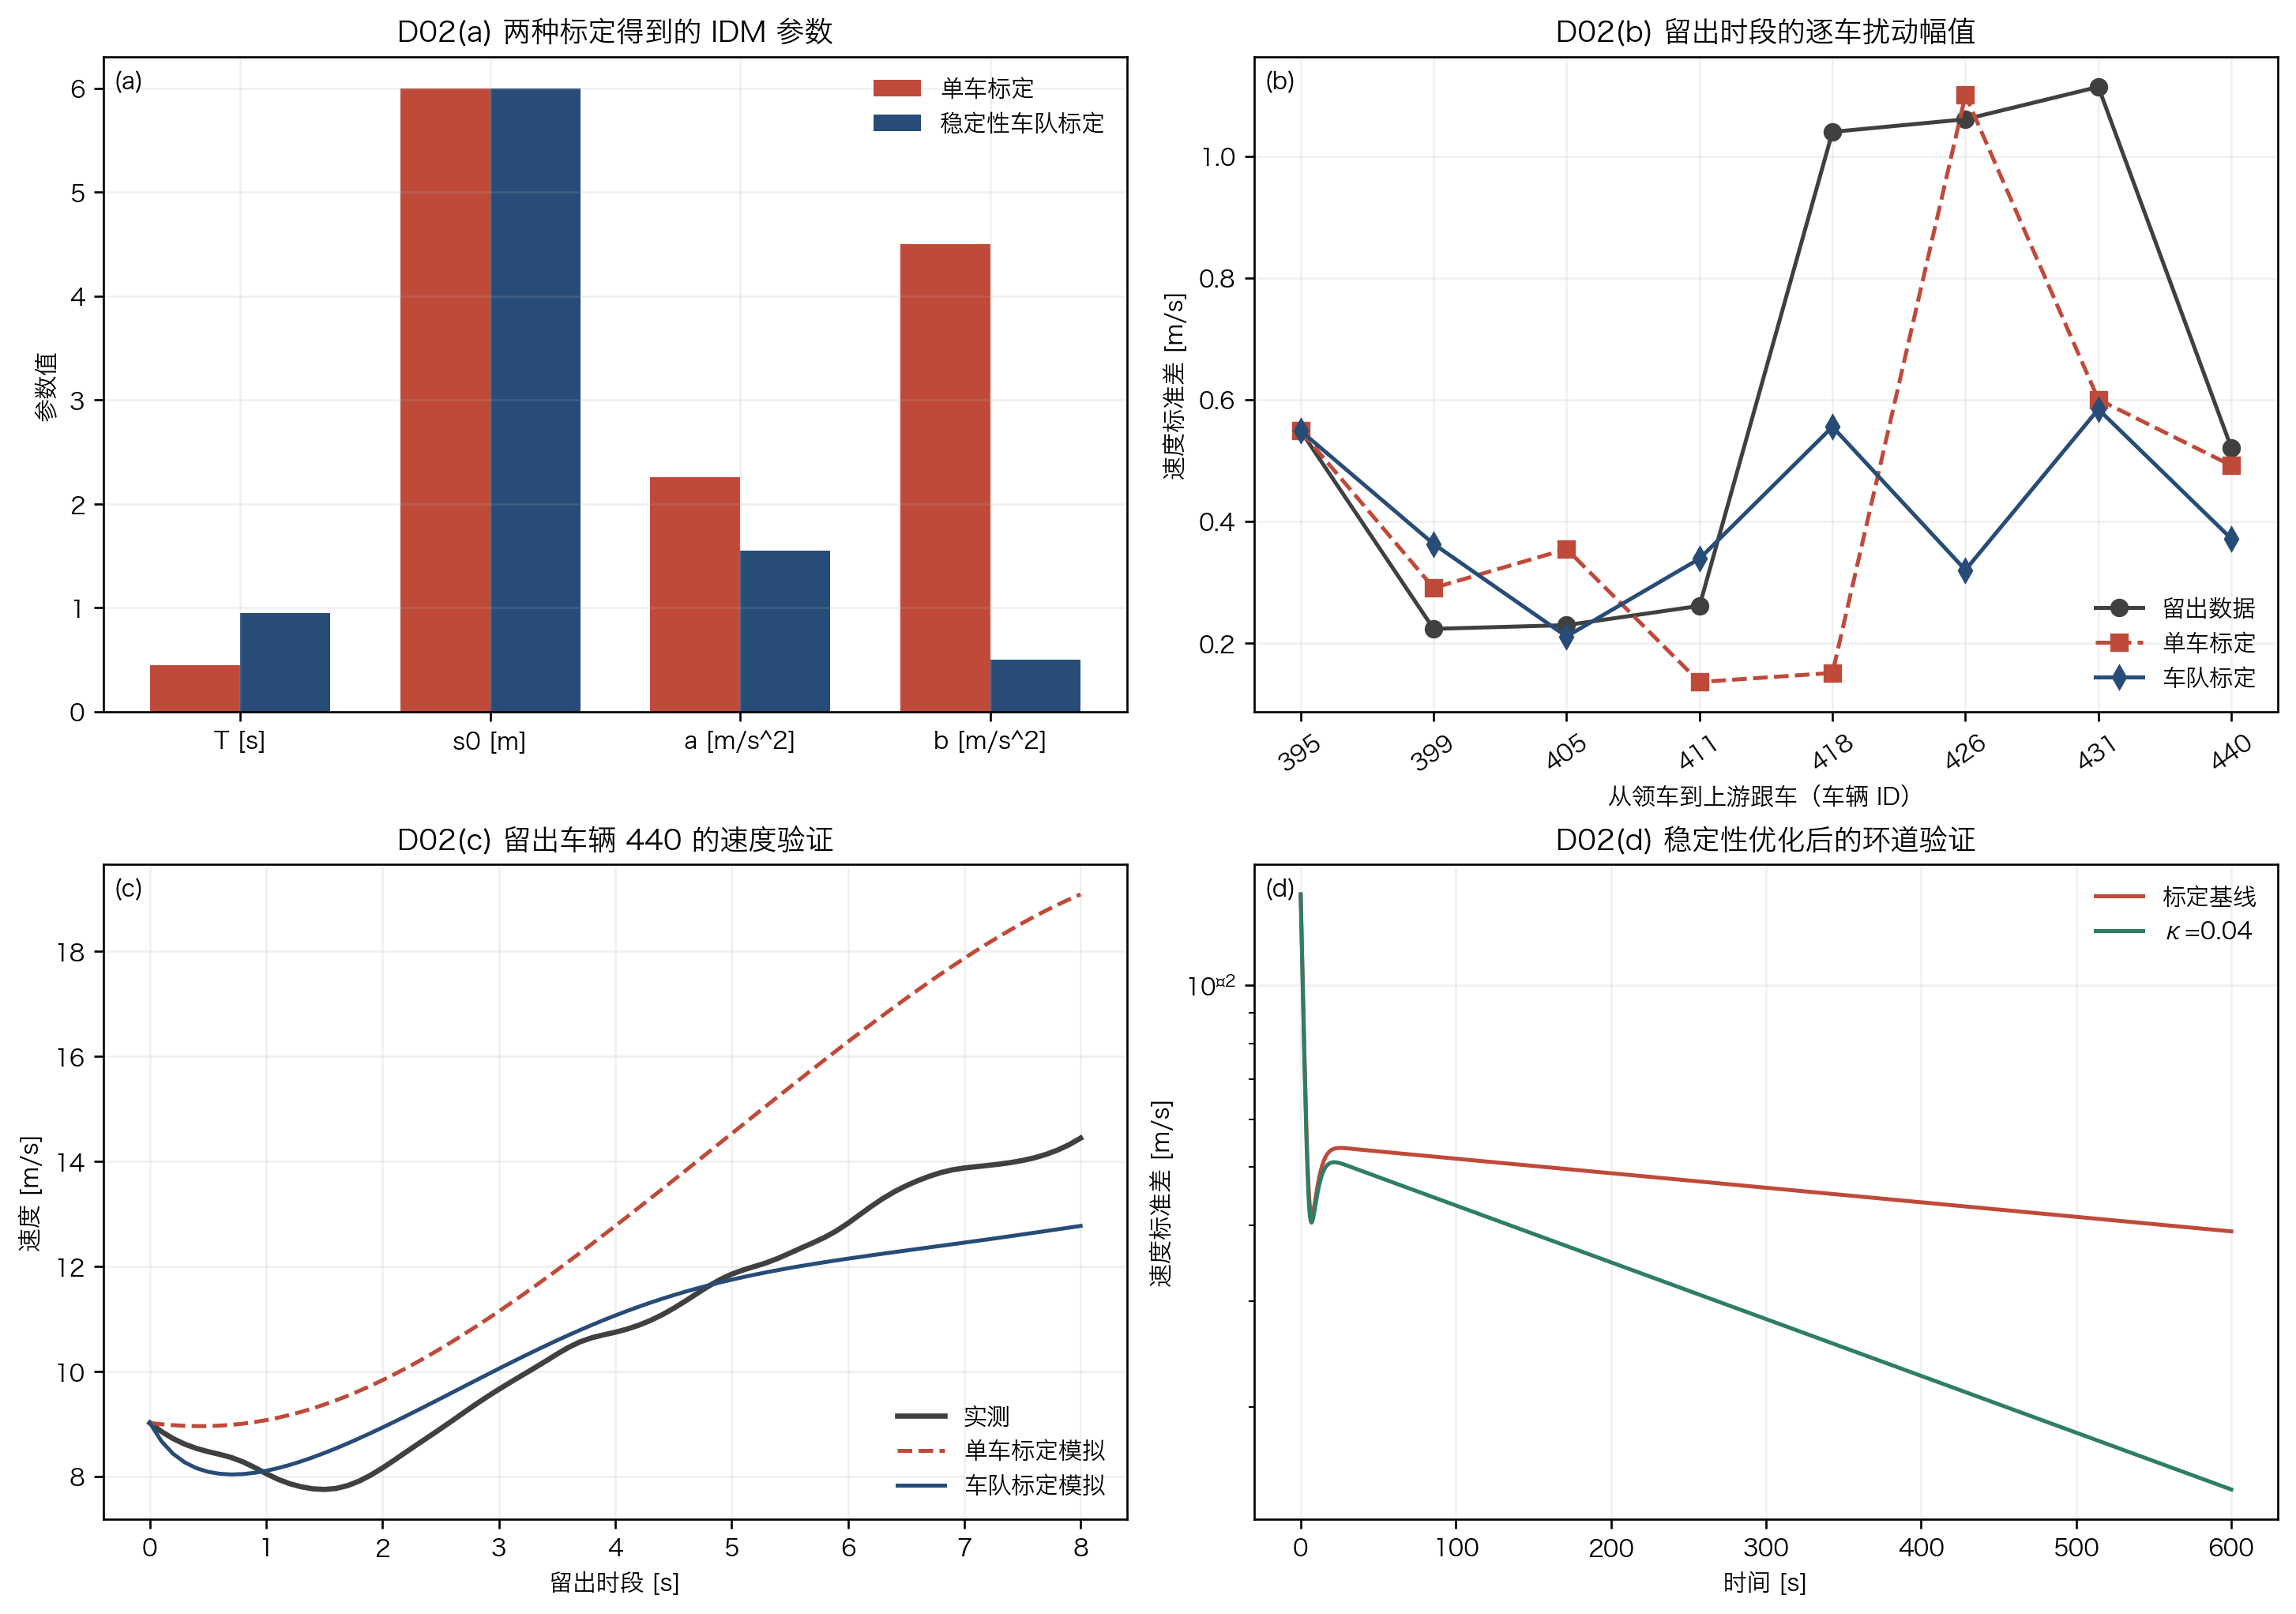
\includegraphics[width=\textwidth]{ngsim_stability_application_d02.png}
\caption{Stability calibration, validation, and control evaluation of NGSIM.}
\label{fig:ngsim-d02}
\figurenote{D02 demonstrates a three-stage process using real data for stability calibration, validation, and control design. Panel (a) compares the parameter results obtained by fitting only the first following vehicle versus simultaneously constraining the trajectories and amplitude profiles of all seven vehicles; the latter better preserves the disturbance pattern within the convoy, indicating that stability information substantially alters the IDM parameters rather than merely renaming the same RMSE. Panel (b) compares per-vehicle amplitudes over a fully reserved 8-second interval, while panel (c) displays the recursive velocity of the lead vehicle, No. 440; fleet calibration significantly reduces velocity and spacing drift but does not improve every propagation statistic, revealing the evidence boundary for short reservation windows. Panel (d) freezes the calibration parameters and selects the minimum intervention $\kappa=0.04$ using spectral constraints at the 5th percentile hazard speed; residual disturbances on the circuit are significantly reduced. This figure demonstrates that stability can be incorporated into model calibration and controller selection, but control gains remain counterfactual with respect to the calibrated model and cannot replace measurements taken on controlled roads.}
\end{figure}

\begin{tcolorbox}[resultbox,title=\textbf{D02 How to Interpret the Three Figures}]
\textbf{Calibration}




Explains how information propagated within the vehicle fleet alters parameters;




\textbf{Reserve for verification}




Explain whether this change can be generalized;







\textbf{Stability optimization}




Explain how to translate spectral constraints into control selection. Only the first two sections are directly constrained by real-world following observations;

the control benefits in the third section are model counterfactuals and must be further validated using data from controlled roads or test tracks.







\end{tcolorbox}

\section{Code, Derived Data, and Traceability}
\sectionstudy{data}{Code, Derived Data, and Traceability}{ngsim2016,thiemann2008,krajewski2018}





The complete entry for D01 is




\texttt{examples/analyze\_ngsim\_us101.py}




; the entry point for D02’s calibration, recursive simulation, spectrum optimization, and plotting is




\texttt{examples/ngsim\_stability\_application.py}




. The former saves the official dataset’s DOI, API fields, time range, unit conversions, filtering window, and random seed, while the latter reads a fixed eight-fleet derived table and outputs




\texttt{ngsim\_stability\_application\_d02.json}




 and the graph ~\ref{fig:ngsim-d02}. The original full dataset is not subject to the code license of this book; the open-source package retains only query scripts and small-scale derived results. See Appendix ~\ref{sec:open-code} for execution commands and directory descriptions.




%==================================================================







\sectionwrapup{D01 Extracted 78 natural drafting events from NGSIM real-world trajectories, with a median gain of 1.033 and a 95 \% interval exceeding 1. D02 further completed stability platoon calibration, reserve recursive simulation, and spectral constraint optimization: Platoon calibration significantly reduced reserve speed/spacing errors but did not improve all propagation metrics; the control gains in $\kappa=0.04$ are counterfactual to the calibrated model and still require controlled field testing for verification.}

\chapter{Applications of Stability Analysis}
\label{sec:applications}
\chapterguide{How Stability Criteria Are Translated into Traffic Management and Control Design}{This chapter uses two complete case studies—an open fleet collaborating with AVs and a fixed upstream VSL—to translate the stability domain, gain, penetration rate, and propagation speed into control choices; safety, efficiency, and energy consumption are evaluated post-simulation to avoid confounding them with online stability objectives.
}










The value of stability analysis extends beyond simply drawing a “stable/unstable” boundary for parameters. It translates vehicle parameters, controllers, communication delays, fleet composition, and test scale into measurable growth rates, gain, dominant wavelength, and recovery time, thereby supporting design, operation, calibration, and validation.










\section{Case Study A: Disturbance Propagation and Cooperative AVs in Open Fleets}
\sectionstudy{application}{Case Study A: Disturbance Propagation and Cooperative AVs in Open Fleets}{milanes2014,talebpour2016,stern2018}


\label{sub:application-open-platoon}




First, consider an open-boundary convoy that directly corresponds to a road-following test. There are $N=60$ vehicles, with a uniform initial velocity of $v_e=8$ m/s, and the initial net spacing is set to the IDM equilibrium value. The lead vehicle begins applying

\begin{equation}
v_0(t)=v_e+0.6\sin\!\left[\frac{2\pi(t-100)}{48}\right],
\qquad 100\le t\le340\ {\rm s},
\label{eq:application-leader-sine}
\end{equation}

at $t=100$ s—a finite-duration sinusoidal disturbance with an amplitude of $0.6$ m/s, a period of $48$ s, and a duration of 5 periods. Since this frequency is close to the peak of the transfer gain for this operating condition, the baseline HDV/IDM fleet will amplify the disturbance upstream; after the disturbance ends, it takes some time for the vehicles to return to uniform flow.




The cooperative AV control group uses acceleration feedforward from three leading vehicles and speed feedback from one trailing vehicle:

\begin{equation}
\dot v_n
=F_n+\sum_{j=1}^{3}\kappa\alpha^{j-1}\dot v_{n-j}
+\gamma\sum_{j=1}^{3}\alpha^{j-1}(v_{n-j}-v_n)
+\eta(v_{n+1}-v_n),
\label{eq:application-cooperative-av}
\end{equation}

where $\kappa=0.34$, $\alpha=0.52$, $\gamma=0.045$, and $\eta=0.055$; only actual neighboring vehicles are retained at the boundaries. This controller represents a communication scenario where “information from multiple leading vehicles is used to anticipate disturbances in advance, while information from the following vehicle is used to suppress speed dispersion within the convoy.” It does not alter the lead vehicle’s input; therefore, the differences between the two groups can be attributed to the nature of disturbance propagation rather than differing external requirements.










\begin{center}
\small
\captionof{table}{Stability benefits of the cooperative AV in Case A.}
\label{tab:application-av-benefits}
\begin{tabular}{p{4.2cm}rrp{4.4cm}}
\toprule
\textbf{Metrics} & \textbf{HDV/IDM} & \textbf{Cooperative AV} & \textbf{Stability Benefits} \\
\midrule







Rear Vehicle Speed Amplitude [m/s]& $0.927$ & $0.099$ & Decrease $89.3\%$; Propagation gain from $1.545$ to $0.165$



\\







Peak velocity standard deviation [m/s]




& $0.549$ & $0.193$ &




 Descent $64.9\%$



\\







 Recovery time [s]




& $454$ & $392$ &




 Advance $62$ s



\\







Minimum net clearance [m]




& $12.59$ & $13.11$ &




 Increased clearance margin



\\







Minimum TTC [s]




& $65.3$ & $116.2$ &




 Small disturbance safety margin increase $78.0\%$



\\







Wu model disturbance additional power consumption [Wh/vehicle]




& $0.718$ & $0.076$ &




 Decrease $89.4\%$



\\







Net energy consumption per mile [kWh/100 km]




& $4.412$ & $4.405$ &




 Decrease $0.15\%$



\\
\bottomrule
\end{tabular}
\end{center}
\tabletext{tab:application-av-benefits}{




Propagation, recovery, safety agent, and energy consumption results for the pure HDV and the collaborative AV fleet under the same lead-vehicle sinusoidal disturbance. The amplitude of the trailing vehicle and the additional energy consumption due to disturbances both decrease by approximately $89\%$, while the total energy consumption per unit distance changes only slightly, indicating that the stabilizing control primarily eliminates the marginal losses caused by repeated acceleration and deceleration.}





To avoid mistaking $v\max(\dot v,0)$ for actual energy consumption, this book adopts the EV instantaneous power model \cite{wu2015ev} developed by Wu et al. and validated using real-world vehicle data. Given the speed $v$, acceleration $a$, and gradient $\theta$, first calculate the traction force

\begin{equation}
F_{\rm tr}=ma+kv^2+f_{\rm rl}mg+mg\sin\theta,
\label{eq:wu-tractive-force}
\end{equation}

The power on the battery side is expressed as

\begin{equation}
P_{\rm EV}
=\frac{rR^2}{K^2}F_{\rm tr}^{\,2}
+v\!\left(kv^2+f_{\rm rl}mg+mg\sin\theta\right)+mav,
\qquad
E_{\rm EV}=\int_0^{T_f}P_{\rm EV}(t)\,{\rm d}t.
\label{eq:wu-ev-power}
\end{equation}

The first term represents motor copper losses; the second term represents the power required to overcome air, rolling, and gradient resistance; the third term represents the change in kinetic energy; $P_{\rm EV}<0$ represents regenerative braking recharge. For this example, the actual vehicle parameters from Table ~1 of this paper are used: $m=1266$ kg, $f_{\rm rl}=0.006$, $k=1.30$ kg/m, $K=10.08$ V, $\cdot$ s, $r=0.11\ \Omega$, $R=0.50$ m, and let $\theta=0$. The absolute energy consumption values presented here correspond to the modified test vehicle used by Wu et al. and cannot be directly applied to any mass-produced EV; the average absolute error across the 41 trips in the original study was $15.6\%$. Therefore, this book primarily uses relative changes measured for the same vehicle, on the same route, and within the same time window.




“Disturbance-induced additional energy consumption” is defined as the energy consumption of the complete trajectory minus the energy consumption of the same vehicle traveling at a constant speed of $v_e=8$ m/s for 1200 s. The average speeds of the HDV and AV are nearly identical, and their total energy consumption per unit mileage differs by only $0.15\%$;However, the additional energy consumption directly related to repeated acceleration and deceleration decreased from $0.718$ to $0.076$ Wh/vehicle, a reduction of $89.4\%$. This distinction is important: stability control significantly eliminates




\cnemph{marginal losses caused by disturbances}




, but it does not eliminate the primary energy required to maintain baseline cruising. The TTC values also fall within the non-hazardous range, indicating an improvement in the relative safety margin; to evaluate collision risk, one should instead use more aggressive braking magnitudes and incorporate braking saturation and perception errors.










\begin{figure}[htbp]
\centering
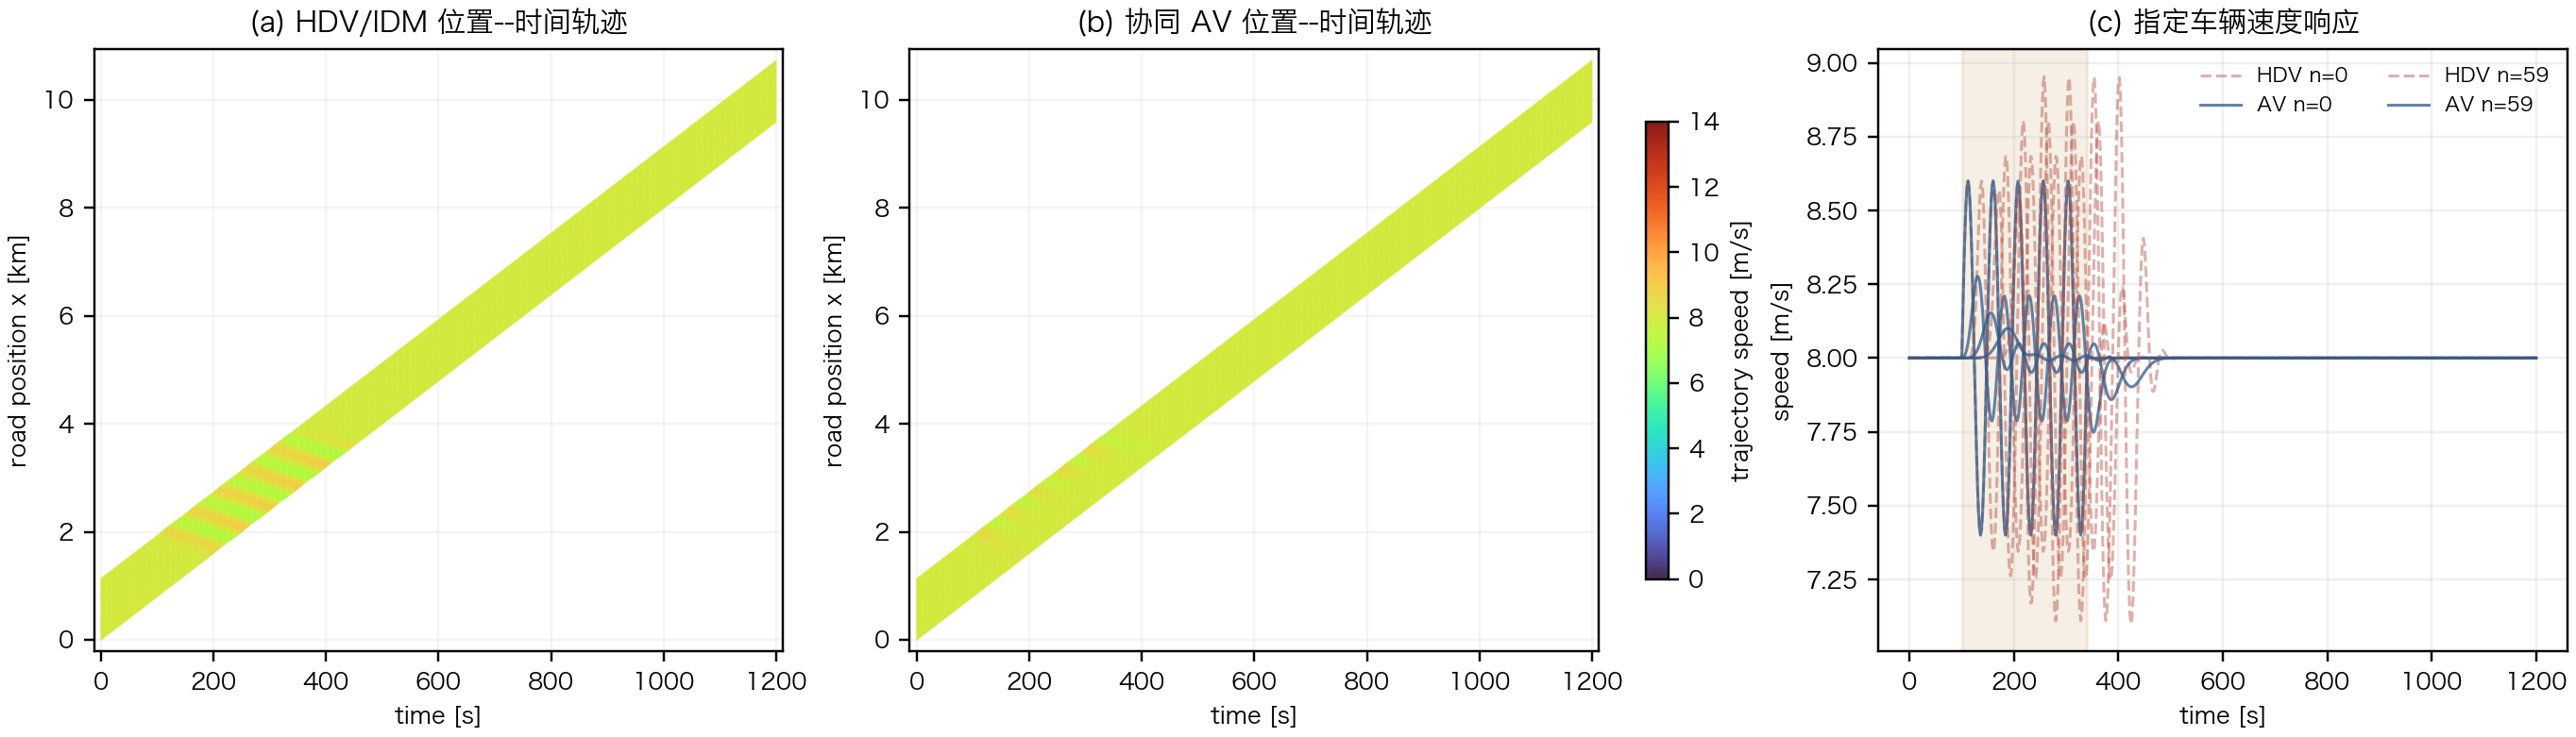
\includegraphics[width=\textwidth]{application_open_platoon.png}
\caption{Case A: Cooperative AV stabilization in an open fleet.}
\label{fig:application-open-platoon}
\figurenote{Case A illustrates the different propagation consequences of the same open-fleet input under pure HDV and cooperative AV conditions. The lead vehicle applies a sinusoidal disturbance with an amplitude of 0.6 m/s, a period of 48 s, and a total of 5 cycles starting from $t=100$ s, after which it returns to constant speed; The position-time plots on the left and in the center use the same speed color scale, allowing for a direct comparison of the width and duration of the colored wavebands along the actual road coordinates. In the pure HDV scenario, the waveband widens vehicle by vehicle toward the upstream vehicles, and significant residual oscillations persist even after the lead vehicle’s input ceases; in the cooperative AV scenario, the waveband narrows due to the use of multi-vehicle anticipation and speed feedback from trailing vehicles, and it quickly returns to a uniformly colored, oblique straight trajectory. The curve for the specified vehicle on the right further shows that the amplitude of the rear vehicle decreased from 0.927 to 0.099 m/s, the propagation gain decreased from 1.545 to 0.165, and the recovery time was brought forward by 62 s. In conjunction with Table ~\ref{tab:application-av-benefits}, this figure demonstrates that the stabilization technique not only reduces visual fluctuations but also simultaneously lowers speed dispersion, minimizes disturbance-induced energy consumption, and improves spacing accuracy; however, these safety and energy-saving benefits are evaluated post-simulation and are not guaranteed by any single linear criterion.
}
\end{figure}

\section{Specific Case B: Low-Speed Vehicles in Continuous Traffic Flow and Variable Speed Limit Zones with Fixed Geometric Configurations}
\sectionstudy{application}{Specific Case B: Low-Speed Vehicles in Continuous Traffic Flow and Variable Speed Limit Zones with Fixed Geometric Configurations}{hegyi2005,carlson2010}


\label{sub:application-moving-bottleneck}




The second case uses a continuous, open traffic flow and maintains the statutory maximum speed limit on the highway of $120$ km/h. To construct a true linear instability scenario at high speeds as suggested by readers, this book only reduces the IDM-expected headway from the baseline value to $T=0.7$ s; all other IDM parameters remain unchanged. Given a net spacing of $s_e=18$ m and a vehicle length of $l=5$ m, the uniform equilibrium speed corresponding to $v_0=120$ km/h is $v_e=74.95$ km/h, with a flow rate of approximately $3261$ veh/h. This flow rate exceeds the typical single-lane capacity of manually driven vehicles; therefore, it should be interpreted as a




\textbf{theoretical validation scenario characterized by short headways and high demand.}, rather than standard HDV capacity calibration. Between $0$ and $1200$, vehicles continuously entered and exited downstream, with a total of 1,087 new vehicles crossing the upstream boundary.




Vehicle No. 533 reached a point approximately $t=300$ s at $x_b=6$ km and, between $300$ and -$420$ s, it reduced its target speed from approximately $75$ km/h to $18$ m/s ($64.8$ km/h). This is only a disturbance of approximately $10$ km/h for a limited duration; however, because the small $T$ operating point satisfies $\Phi<0$, the disturbance is amplified and forms a queue tail that propagates noticeably upstream. This allows us to distinguish between “amplification caused by stability” and “direct road closure due to an extreme incident.”




The VSL does not uniformly adjust parameters for “all upstream vehicles,” nor does it follow the slow vehicle’s movement. It is fixed 1 km upstream of the point where the slow vehicle begins to decelerate at $x_b^0=6$ km:

\begin{equation}
\Omega_{\rm VSL}=\bigl[x_b^0-1000,\ x_b^0\bigr)
= [5000,6000)~{\rm m},
\qquad 300\le t\le900~{\rm s}.
\label{eq:vsl-fixed-zone}
\end{equation}

Vehicles only accept speed limit commands when they are at their own position $x_n(t)\in\Omega_{\rm VSL}$. More importantly, the VSL is strictly deactivated at $t<300$ s; roadside detection only triggers control after the slow-moving vehicle begins to decelerate at $t=300$ s. Consequently, this simulation no longer includes any preemptive speed limits in anticipation of accidents.After the slow train departs 6 km from the event point, the VSL remains within a fixed 5–6 km section; it is not tied to a specific train number, nor does it move along the slow train’s trajectory. Figure ~\ref{fig:application-moving-bottleneck}(f) simultaneously plots the slow train’s trajectory and the fixed spatial band, which gradually diverge after the event occurs.










\subsection{Directly Maximizing the Stability Margin Within Permissible Limits}










The VSL target displayed on the road management interface is denoted as $u$; in this example, the IDM desired speed parameter is set directly to $v_0=u$. The statutory speed limit for the road remains $120$ km/h. Fix the current net headway at $s_e=18$ m. For each operationally permitted target of $u\in\mathcal U=[114,120]$ km/h, first calculate the new uniform equilibrium speed $v_e(u)$:

\begin{equation}
F\!\left(s_e,v_e(u),0;v_0=u,T=0.7~{\rm s}\right)=0,
\label{eq:vsl-new-equilibrium}
\end{equation}

Then calculate the long-wave margin at this new equilibrium point

\begin{equation}
\Phi(u)=\frac12\left[f_v(u)^2-f_{v_l}(u)^2\right]-f_s(u).
\label{eq:vsl-phi}
\end{equation}

The allowable range $\mathcal U$ is an online control constraint predefined by the administrator; within this range, the objective function includes only




\textbf{stability measures}




:

\begin{equation}
u^*=\arg\max_{u\in\mathcal U}\Phi(u).
\label{eq:vsl-stability-only-objective}
\end{equation}

Here, the minimum margin that “just exceeds the threshold” is no longer selected; instead, the maximum $\Phi$ is directly taken within the allowed speed band. Neither the minimum TTC, queuing, delay, nor energy consumption are included in the expression ~\eqref{eq:vsl-stability-only-objective}; these metrics can only be evaluated retrospectively through a full simulation after the control values have been determined.





\begin{center}
\small
\captionof{table}{Stability margin for the VSL candidate speed.}
\label{tab:vsl-candidates}
\begin{tabular}{rrrr}
\toprule
$u$ [km/h] & $v_e(u)$ [km/h] & $\Phi(u)$ [s$^{-2}$] &




 Linear conclusion



\\
\midrule
\textbf{114} & \textbf{73.78} & \textbf{$+0.002396$} & \textbf{Stable, maximum margin} \\
115 & 73.98 & $+0.001727$ &




 Stable



\\
116 & 74.19 & $+0.001071$ &




 Stable



\\
117 & 74.39 & $+0.000429$ &




 Stable



\\
118 & 74.58 & $-0.000199$ &




 Instable



\\
119 & 74.77 & $-0.000814$ &




 Instable



\\
120 & 74.95 & $-0.001415$ &




 Instable



\\
\bottomrule
\end{tabular}
\end{center}
\tabletext{tab:vsl-candidates}{




114–120 km/h: The re-calculated equilibrium speed and analytical margin for each candidate speed limit within the operational tolerance band. The margin becomes negative starting at $u=118$ km/h, while $u=114$ km/h yields the maximum positive margin within the feasible set; therefore, the control variable is derived from stability optimization rather than ex post safety or delay metrics.}





Without control, the legal limit $u=120$ km/h corresponds to $\Phi=-0.001415$ s$^{-2}$, which is indeed on the side of linear instability. Maximizing the expression ~\eqref{eq:vsl-stability-only-objective} yields $u^*=114$ km/h and $\Phi=+0.002396$ s$^{-2}$; reducing $6$ km/h alone is sufficient to move the operating point into the stable region. The lower bound of $114$ km/h is a predefined operational constraint for a one-kilometer control zone; it is not derived from safety or delay simulations. The event and control are triggered simultaneously at $t=300$ s, and the command is smoothly phased out over $300$--330$ s, begins smoothly, and is phased out over $810$--900$ s; The vehicle adapts to the target speed along a spatial gradient within a fixed 5–6 km zone to avoid artificially creating a step impact at the entrance. The term “simultaneous triggering” here refers to idealized, instantaneous detection; to study communication and detection delays, a positive trigger delay should be set and the simulation rerun—the control must not be advanced to occur before the event.










\subsection{Post-simulation evaluation: It is not possible to retroactively simulate online targets.}





To directly measure the propagation direction, define the tail of the low-speed queue

\begin{equation}
x_q(t)=\min\{x_n(t):v_n(t)<18.2~{\rm m/s}\},
\qquad c_q=\frac{{\rm d}x_q}{{\rm d}t}.
\label{eq:vsl-queue-tail-speed}
\end{equation}

$c_q<0$ to indicate that the tail propagates upstream. This book fits $c_q$ to the linear segment between $360$ and $420$. The remaining queueing, safety, delay, and energy consumption are all calculated based on two complete continuous-flow simulations




\textbf{post-simulation calculations}




, without the entry-type ~\eqref{eq:vsl-stability-only-objective}.










\begin{center}
\small
\captionof{table}{Post-simulation evaluation of VSL for Case B.}
\label{tab:vsl-post-evaluation}
\begin{tabular}{p{4.2cm}rrp{4.4cm}}
\toprule
\textbf{Metrics} & \textbf{No Control} & \textbf{Stability-Constrained VSL} & \textbf{Results} \\
\midrule







Newly Arriving Vehicles Within 1200 s




& $1087$ & $1087$ &




The boundary demands of the two groups are exactly the same



\\







Vehicles exiting downstream




& $1072$ & $1072$ &




Both groups are identical



\\







Traffic tail speed during the formation phase $c_q$ [m/s]




& $-2.687$ & $-0.284$ &




 Decrease in the absolute value of the reverse propagation speed $89.4\%$



\\







Peak speed of low-speed vehicles ($v<18.2$ m/s)& $121$ & $102$ &




 Abstieg $15.7\%$


















\\







Peak velocity standard deviation [m/s]




& $8.912$ & $4.107$ &




 Decrease $53.9\%$



\\







Minimum net spacing [m]




& $1.56$ & $3.27$ &




 Increase by approx. $109.8\%$



\\







Minimum TTC [s]




& $2.34$ & $6.70$ &




 Approximate increase $186\%$



\\







Cumulative delay [veh$\cdot$h]




& $6.866$ & $4.799$ &




 Decrease $30.1\%$



\\







Net energy consumption per mile [kWh/100 km]




& $17.521$ & $17.328$ &




 Decrease $1.10\%$



\\
\bottomrule
\end{tabular}
\end{center}
\tabletext{tab:vsl-post-evaluation}{




Complete simulation results for the uncontrolled and event-triggered VSL under the same continuous arrival demand. Control remains off before the slow vehicle disturbance occurs; After triggering, the absolute value of the negative tail-wave velocity decreases $89.4\%$, while queue size, velocity dispersion, delay, and safety performance improve. These values are used to validate the speed limit selected by $\Phi$, without reverse participation in the online target.}





In the uncontrolled position-time plot, the black dashed line slopes noticeably from $x=6$ km toward the smaller value of $x$; The value of $c_q=-2.687$ m/s, fitted during the formation phase of $360$–$420$ s, clearly demonstrates that the congestion wake propagates upstream. The event-triggered VSL does not alter any vehicles prior to $t=300$ s; only after triggering does it push the upstream operating point from $\Phi<0$ toward $\Phi>0$. The low-speed band in the control chart narrows significantly, and the absolute value of the slope at the tail of the formation phase decreases to $0.284$ m/s; peak speed deviation decreases by $53.9\%$, cumulative delay decreases by $30.1\%$, and the minimum TTC improves from $2.34$ s to $6.70$ s. Compared to the previous results that included precontrol, the gains are somewhat reduced, but the causal sequence remains correct. It should still be emphasized that:




\textbf{Only $\Phi$ meets the online target; wake velocity, queuing, safety, delay, and energy consumption are all results verified a posteriori, rather than theoretically guaranteed in advance.}

\begin{figure}[htbp]
\centering
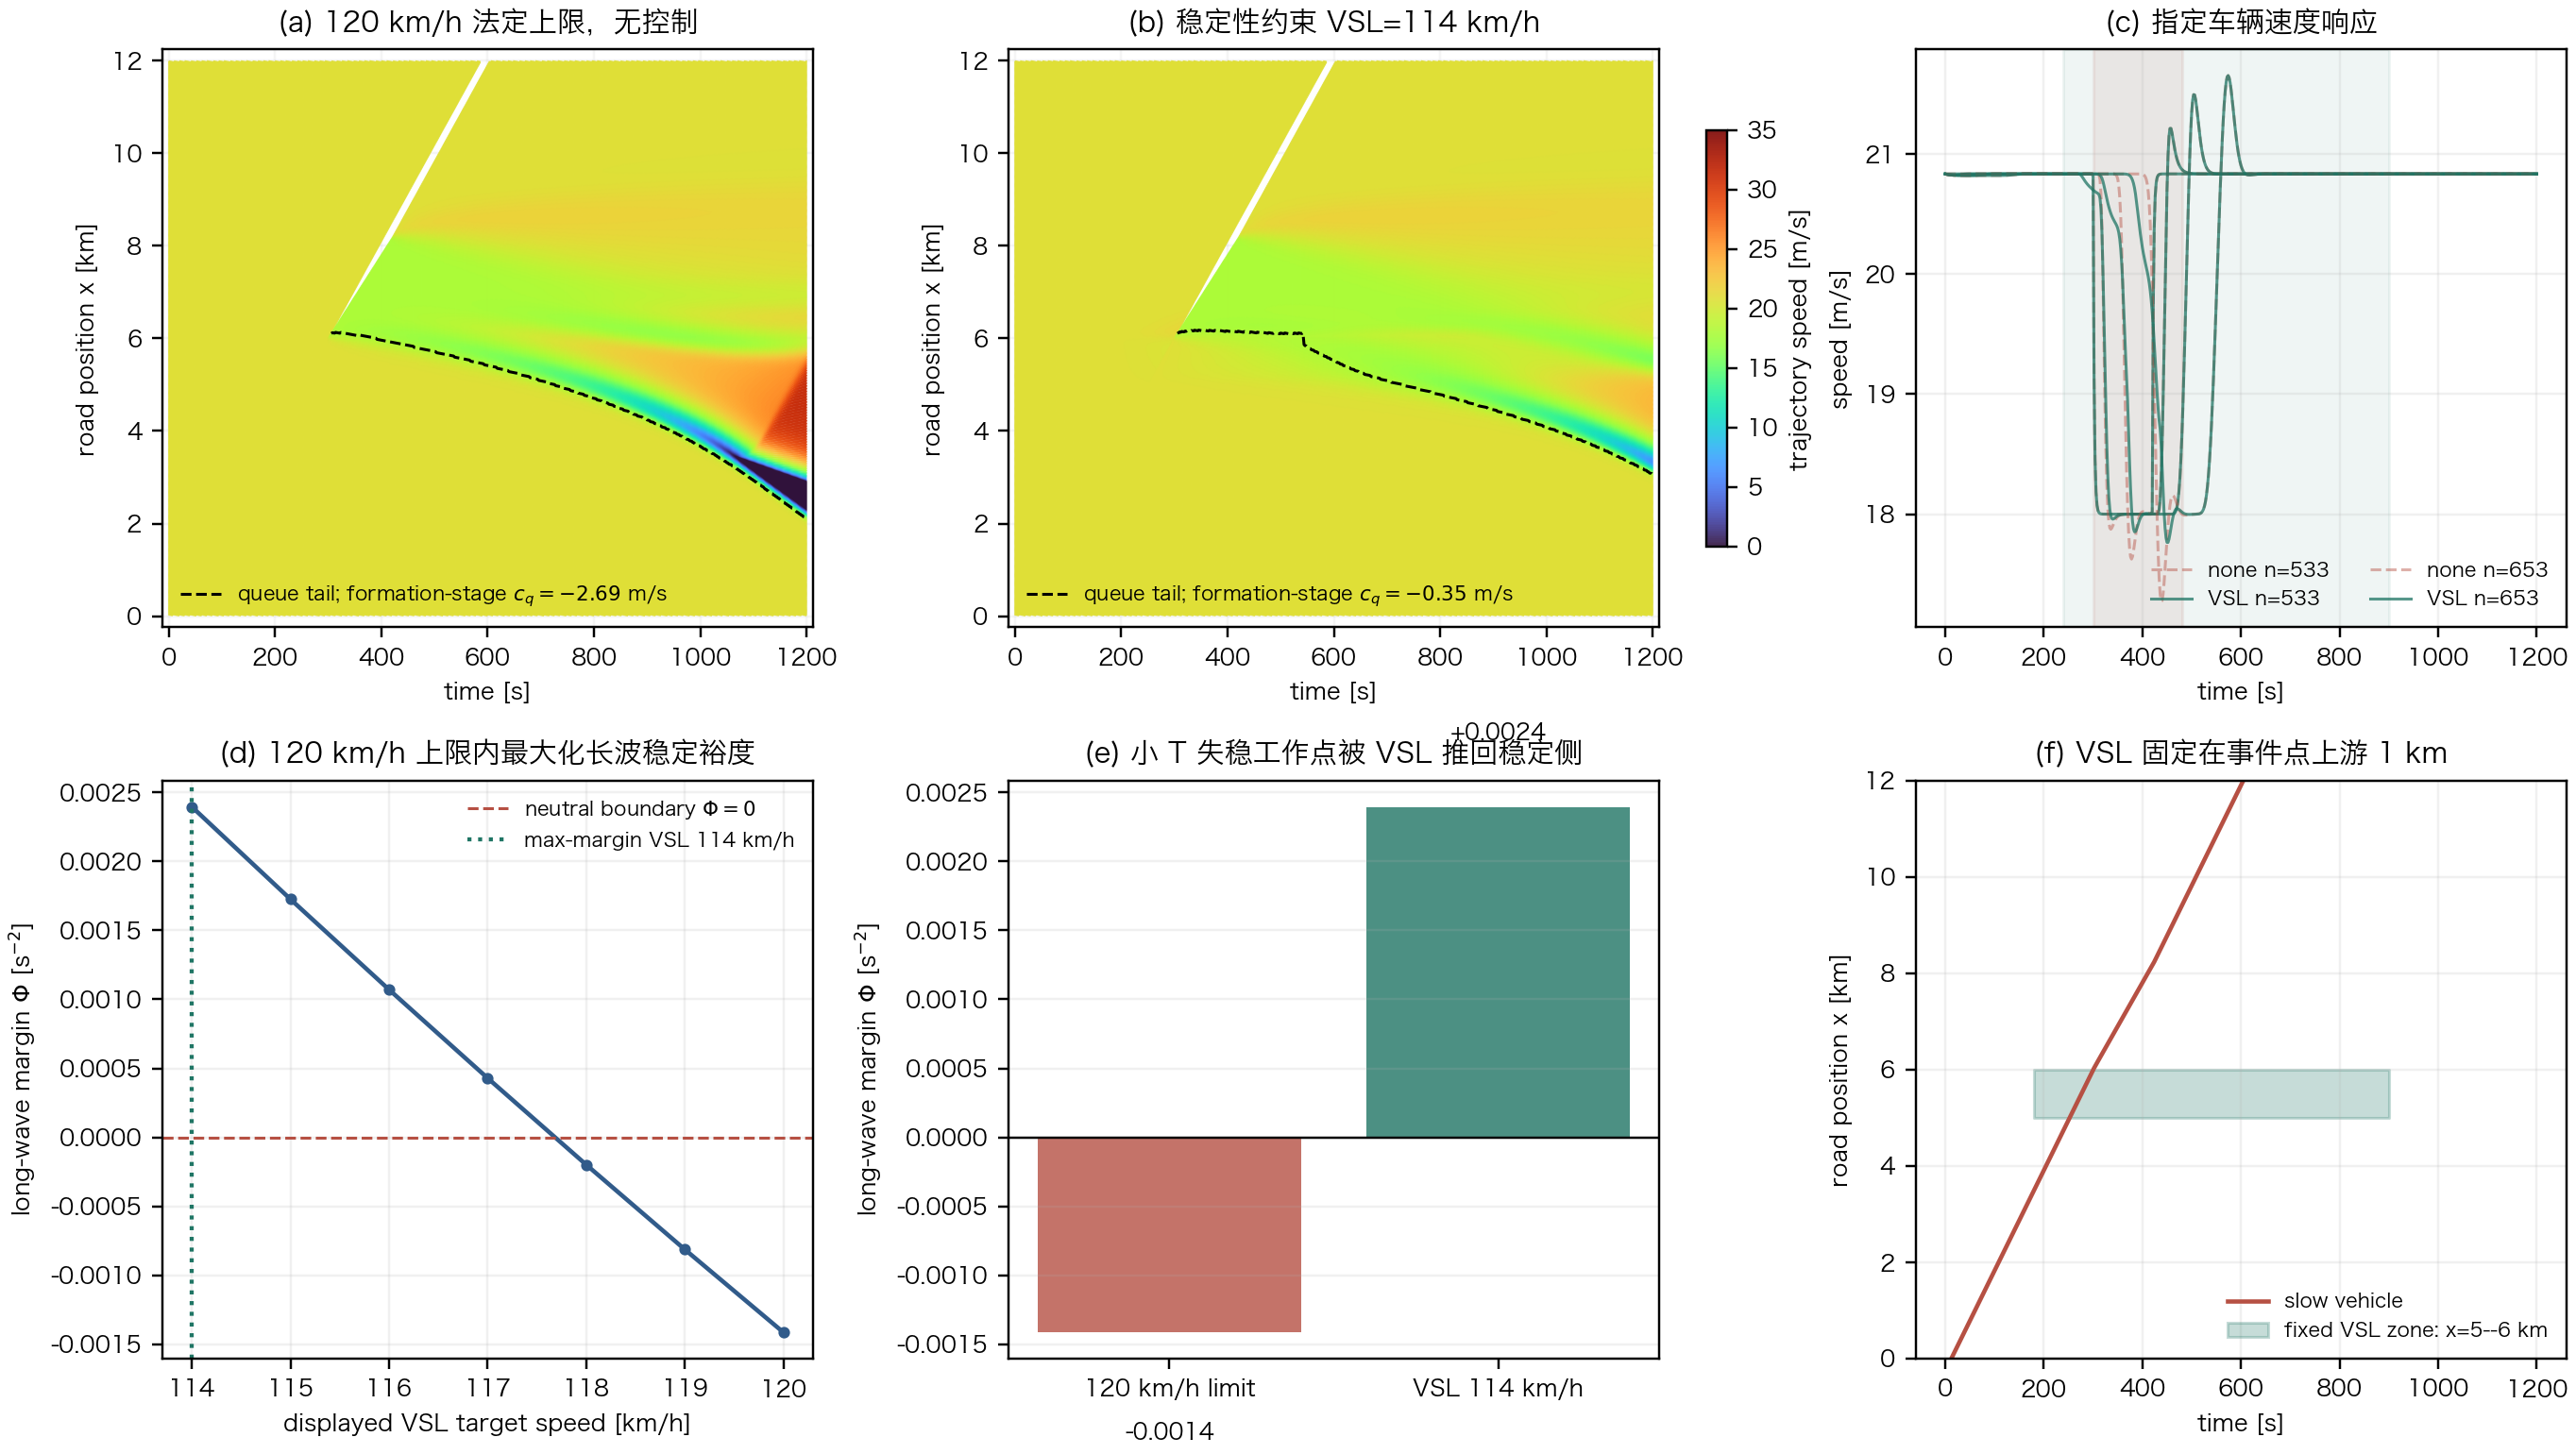
\includegraphics[width=\textwidth]{application_moving_bottleneck.png}
\caption{Case B: Fixed-area VSL based on maximum stability margin.}
\label{fig:application-moving-bottleneck}
\figurenote{Case Study B demonstrates how stability constraints are translated into a fixed-space, event-triggered VSL, and verifies its road benefits through a full continuous-flow simulation. Within $0$--$1200$ s, upstream demand continues to arrive, the statutory speed limit remains at 120 km/h; a short time interval of $T=0.7$ s keeps the flow uniform at $\Phi<0$, and slow-moving vehicle No. 533 triggers a disturbance near $t=300$ s and $x=6$ km. At $t<300$ s, VSL is strictly deactivated; subsequently, a control zone fixed at $x=5$–$6$ km appears but does not follow the slow train. In the uncontrolled diagram, the low-speed tail tilts toward the smaller $x$, with a fitted speed of $c_q=-2.687$ m/s. Among the candidate speed limits, only those within the range of 114–120 km/h exhibit a relatively large analytical margin; $u^*=114$ km/h causes $\Phi$ to change from $-0.001415$ to $+0.002396$. Upon triggering, the low-speed band in the control diagram narrows, and the absolute value of the wake velocity drops to 0.284 m/s; Table ~\ref{tab:vsl-post-evaluation} shows a discrete decrease in velocity of 53.9




\%




and a cumulative delay reduction of 30.1\%. This figure illustrates that stability constraints can still mitigate disturbance amplification even without pre-control, while queuing, safety, delays, and power consumption are merely ex post evidence after the control values have been determined.
}
\end{figure}

\begin{tcolorbox}[resultbox,title=\textbf{Two case studies illustrate how stability analysis aids traffic management}]
\begin{itemize}[leftmargin=1.4em,itemsep=3pt]
\item




For vehicle-level control, line stability provides a preliminary screening to determine whether “perturbations will amplify on a vehicle-by-vehicle basis”; time-domain simulation then converts spectral margins into safe following distances, recovery times, and energy consumption according to the Wu model.







\item




For roadside management, the equilibrium point and stability region must be recalculated for each candidate speed limit; the online objective function uses only the stability margin $\Phi$, while position-time trajectories, queues, safety, delays, and energy consumption serve as post-hoc verification.







\item




Control evaluations must report both benefits and costs. Displaying only smoother speed heatmaps without reporting delays, recovery times, and energy consumption may misrepresent “temporarily shifting congestion upstream” as “eliminating congestion.”







\end{itemize}







The “Application Cases” tab on the test bench provides two sets of uncontrolled/controlled position-time trajectories, specified vehicle speed curves, VSL scans, and the aforementioned quantitative readings, which correspond item by item to Figure ~\ref{fig:application-open-platoon} and Figure ~\ref{fig:application-moving-bottleneck}.







\end{tcolorbox}

\section{Application 1: Gain Design for ACC/CACC Controllers}
\sectionstudy{application}{Application 1: Gain Design for ACC/CACC Controllers}{milanes2014,talebpour2016,stern2018}





Control design should proceed in the following order: “Long-wave budget $\rightarrow$, full-band constraints $\rightarrow$, and time-domain verification.” For lead-vehicle acceleration feedforward, the first step is to determine the minimum gain required for the operating point using

\begin{equation}
\kappa_{\min}(v_e)
=1-\frac{f_v^2-f_{v_l}^2}{2f_s}
\label{eq:application-kappa}
\end{equation}

, then check $|\kappa|\le1$ and $\Psi(\omega)\ge0$ under communication delay. The worst-case value across the full speed range for the benchmark IDM in this book is $\kappa_c=0.134$; therefore, selecting $\kappa=0.15$ is sufficient to ensure that the growth rates of $v_e=8$ m/s and and $m=4$ from $+0.00408566$ s$^{-1}$ to the rightmost mode $-1.14052\times10^{-4}$ s$^{-1}$. The linear doubling time for the former is only

\begin{equation}
t_2=\frac{\ln2}{0.00408566}=169.7\ \text{s},
\end{equation}

, meaning the disturbance can double in about three minutes; after stabilization, it transitions to a slow decay.




From an engineering perspective, one cannot simply select a gain that is “just above the critical threshold.” If $\kappa$ is too close to $0.134$, parameter errors, sampling delays, and vehicle model variations may all erode the margin; if $\kappa$ is too large, it will approach the high-frequency upper bound. A reasonable approach is to maximize the minimum spectral margin across the speed-density operating domain, while incorporating constraints related to acceleration, comfort, and actuator bandwidth.










\section{Application 2: AV Penetration Rate and Fleet Deployment in Mixed Traffic}
\sectionstudy{application}{Application 2: AV Penetration Rate and Fleet Deployment in Mixed Traffic}{milanes2014,talebpour2016,stern2018}





The long-wave index $\eta_n$ for a heterogeneous fleet can be directly converted into a penetration budget. This book derives the total long-wave budget threshold for the entire team/circuit, $26.7\%$, from $\kappa=0.5$; it only guarantees $S_N\ge0$, and open teams must still check all $S_j$. AVs can only obtain full V2V feedforward when the leading vehicle is also an AV,




\textbf{The same penetration rate arrangement will also alter the total stability budget}。$N=120$、30\%




For AVs at $v_e=9$ m/s, the closed-loop results yield $n_{\rm grp}^{\max}=5.6$: dividing into a maximum of 5 groups ensures the total budget first, then distributes vehicles as evenly as possible within this constraint to reduce mid-route peaks.




Such conclusions can be applied to fleet formation, dedicated lane entry sequencing, and cooperative cruising activation strategies: first ensure a sufficient number of adjacent AV–AV pairs, then optimize vehicle dispersion, rather than simply reporting an “average permeability” that is independent of the arrangement.




Engineering deployments should also use the two-dimensional stability region of \ref{fig:av-stability-plane}—$p_{\rm AV}$–$v_e$, rather than treating $26.7\%$ as a constant applicable to all speeds and all arrangements. The actual process involves reading the most unfavorable boundary within the target speed band and allowing positive margins of $M_{\rm L}$ and $M_{\rm T}$ for $\kappa_0$, the number of trainsets, and arrangement uncertainties.










\section{Application 3: Online Congestion Early Warning and Control Triggering}
\sectionstudy{application}{Application 3: Online Congestion Early Warning and Control Triggering}{milanes2014,stern2018,hegyi2005}










During actual operation, speed deviations and the dominant Fourier mode can be calculated within a rolling time window:

\begin{equation}
\widehat g(t)=\frac{\mathrm d}{\mathrm dt}\ln\sigma_v(t),
\qquad
\widehat m^*(t)=\arg\max_m|A_m(t)|.
\label{eq:online-indicators}
\end{equation}

If $\widehat g$ remains positive, the dominant mode remains consistent across adjacent windows, and the amplitude remains within the linear region, control can be triggered before a full stop-and-go wave forms. In the online dry run example in Chapter ~\ref{sec:protocol}~, $\kappa$ is smoothly increased from 0 to 0.45 starting at $t=600$ s, and the standard deviation of velocity decreases from approximately $0.534$ m/s after formation to $0.018$ m/s, indicating that stability metrics can serve not only as offline criteria but also as online trigger conditions.




To avoid misclassifying an isolated braking event as self-excited instability, an early warning must satisfy at least three conditions simultaneously: a positive growth rate, persistence of the spatial mode, and propagation of the disturbance across multiple vehicles; a single-point decrease in speed is not sufficient on its own.










\section{Application 4: Ring Track Testing and Simulation Scale Design}
\sectionstudy{application}{Application 4: Ring Track Testing and Simulation Scale Design}{milanes2014,stern2018,hegyi2005}





The minimum wave number for a finite loop is $2\pi/N$. If the objective of the study is to estimate the linear stability boundary of an infinite fleet, the test scale must cover dangerous long waves. In the benchmark examples in this book, $N=22$ can only observe an instability band ranging from $1.45$ to $11.43$ m/s, while the continuous limit ranges from $0.91$ to $18.61$ m/s; $N=100$ extends to $0.93$–$18.35$ m/s. Therefore:







\begin{itemize}[leftmargin=1.4em,itemsep=3pt]
\item




 Small loop tracks are suitable for demonstrating wave formation and propagation but are not suitable for directly calibrating thresholds for infinite convoys;







\item




 If the number of vehicles is limited, the closed-form condition for a finite $N$ should be used instead of the continuous limit formula;







\item




 The experimental report must specify $N$, the loop length, the allowed number of waves $k_m$, and the excited modes; it is not sufficient to list only the density.







\end{itemize}

\section{Application 5: Model Calibration and Model Selection}
\sectionstudy{application}{Application 5: Model Calibration and Model Selection}{kesting2008,ossen2009,punzo2012}





If you calibrate the following model using only the root-mean-square velocity error, you may end up with parameters that result in “excellent single-vehicle trajectory fitting but completely incorrect fleet stability.” A more reliable objective function should include the following:

\begin{equation}
J(\theta)=w_1J_{\rm traj}+w_2J_{\rm local}+w_3J_{\rm gain}+w_4J_{\rm wave},
\label{eq:calibration-objective}
\end{equation}

where $J_{\rm traj}$ measures position/velocity trajectory error, $J_{\rm local}$ measures single-vehicle root mean square error, $J_{\rm gain}$ measures vehicle-to-vehicle amplification or growth rate, and $J_{\rm wave}$ measures wave speed and dominant wavelength. Validating $\operatorname{Re}\lambda(k)$ and $|G(i\omega)|$ through independent testing can eliminate parameter sets that, although they fit the data point-by-point, produce false stop-and-go waves or excessive dissipation.




Numerical formats should also be validated as “part of the model”: if recalculating the same operating conditions using $\Delta t$ and $\Delta t/2$ results in significant changes in the growth rate or critical points, this indicates that what was observed was discretization stability rather than vehicle model stability.










\section{Application 6: Trade-offs Between Operating Strategies, Capacity, and Comfort}
\sectionstudy{application}{Application 6: Trade-offs Between Operating Strategies, Capacity, and Comfort}{milanes2014,stern2018,hegyi2005}





Stability margins can be applied to speed recommendations, time-distance management, and road operation zones. Increasing the expected time-distance $T$ of the IDM typically improves stability but reduces capacity; increasing the acceleration feedforward maintains a smaller $T$ but increases the requirements for communication reliability and actuator bandwidth; rear-end distance feedback can simultaneously reduce wave speed but introduces bidirectional coupling and finite wavelength constraints. Therefore, the design objective should not be to maximize stability in isolation, but rather to solve for

\begin{equation}
\max_{\theta}\ \min_{(v_e,\rho)\in\Omega}M_\lambda(\theta;v_e,\rho)
\quad\text{s.t.}\quad
q\ge q_{\min},\ |a|\le a_{\max},\ |j|\le j_{\max},\ \tau\le\tau_{\max},
\label{eq:robust-design}
\end{equation}

—that is, to maximize the worst-case stability margin within the target operating region $\Omega$ while satisfying constraints on capacity, acceleration, jerk, and delay. Stability thus becomes a computable metric within a multi-objective design, rather than an isolated “the higher, the better” criterion.










\section{A Six-Step Process from Analysis to Implementation}
\sectionstudy{application}{A Six-Step Process from Analysis to Implementation}{milanes2014,stern2018,hegyi2005}

\begin{tcolorbox}[keybox,title=\textbf{Recommended Engineering Workflow}]
\begin{enumerate}[leftmargin=1.6em,itemsep=4pt]
\item \textbf{Define the operating domain:}




Specify speed, density, number of vehicles, vehicle type distribution, and delay range, rather than selecting just a single nominal point.







\item \textbf{Find Local Roots:}




First ensure that each vehicle is stable on its own, and record the slowest recovery time and damping ratio.







\item \textbf{Check propagation:}




Use $|G(i\omega)|$ for unidirectional homogeneous models; use $\lambda(k)$ for bidirectional models; use the product of transfer functions or full-matrix eigenvalues for heterogeneous fleets.


\item \textbf{Margin of Safety:}




Do not set parameters at the boundaries of the equal sign; perform sensitivity/robustness scans for calibration errors, delays, and permeability.







\item \textbf{Perform limited-range verification:}




Scan at least three perturbation amplitudes and run the simulation over multiple linear time constants to distinguish between slow decay, nonlinear saturation, and subcritical triggering.







\item \textbf{Closed-loop verification:}




Verify using speed-colored spatiotemporal trajectories, speed/distance fields, and specified probe vehicle curves, and perform the $\Delta t$ convergence check.







\end{enumerate}
\end{tcolorbox}

\begin{tcolorbox}[notebox,title=\textbf{Application Boundaries}]

The criteria in this book apply to longitudinal single-lane following. Lane changes, ramps, traffic lights, gradients, perception errors, communication packet loss, and driver randomness on real roads will continuously introduce external disturbances; “model-line stability” does not equate to “roads that are never congested,” much less collision safety certification. Actual controllers must also independently satisfy requirements for safe following distance, fault degradation, actuator saturation, and formal verification.







\end{tcolorbox}

\sectionwrapup{Stability analysis can convert control parameters into growth rates, propagation speeds, recovery times, and available stability regions. The open-fleet case demonstrates that cooperative AVs can suppress upstream amplification; the fixed-upstream VSL case illustrates that speed limits should be determined jointly by the stability region and operational constraints, while safety, efficiency, and energy consumption benefits must be evaluated through independent simulations.}

\chapter{Extended Discussion: Stability Analysis in Machine Learning and Deep Learning Architectures}
\label{sec:ml-stability}
\chapterguide{How Learning Models Can Be Reintegrated into Classical Stability Theory}{This chapter discusses machine learning approaches such as the Chis model, deep temporal models, multi-vehicle graph networks, and reinforcement learning controllers. The focus is not on introducing the network architectures themselves, but rather on explaining how to extract equilibrium states, Jacobians, propagation gains, and verifiable certificates from learned mappings, and on distinguishing between training stability, prediction stability, traffic flow stability, and closed-loop safety.
}










Machine learning can fit complex driving behaviors from large amounts of trajectory data, but “low prediction error” does not automatically imply “long-term rolling stability,” much less “non-amplification of perturbations along the convoy.” On the other hand, forcibly training all learning models to be linearly stable may also erase the stop-and-go waves that actually exist in human driving data. Therefore, the appropriate role of machine learning in stability analysis is not to replace dynamical systems theory, but to express unknown dynamics, hidden states, or control strategies as differentiable or well-defined operators, which can then be examined by stability tools to assess their temporal evolution and spatial propagation.










\section{First, clarify: Which type of “stability” are we discussing?}
\sectionstudy{synthesis}{Distinctions Among Four Categories of Stability in the Context of Machine Learning}{chen2018neuralode,revay2020contracting,wang2025kidl}










The same term “stable learning” can refer to at least four different concepts.










\begin{center}
\small
\captionof{table}{Four types of stability issues in machine learning traffic models.}
\label{tab:ml-four-stabilities}
\begin{tabular}{p{3.2cm}p{4.2cm}p{6.8cm}}
\toprule
\textbf{Levels} & \textbf{Typical Problems} & \textbf{What to Check} \\
\midrule







Training/Optimization Stability




&




 Whether the loss converges, and whether gradients explode or vanish




&




 Optimization algorithms, gradient statistics, and random seeds; does not directly provide conclusions regarding traffic flow\\

[3pt]

Roll stability of a single model






&






Is the integration of the learned velocity/acceleration model limited over a long period?






&






Jacobian matrix, basin of attraction, and numerical integrator for single-step maps or continuous vector fields





\\

[3pt]

Traffic flow stability






&






Does a vehicle disturbance amplify over time or along the platoon of vehicles?

&

Ring-road mode $\lambda(k)$, discrete step map $M(k)$, transmission gain, and finite-amplitude spatiotemporal diagram





\\

[3pt]

Stability of the learning controller in the closed-loop system






&






Is the neural strategy stable when integrated into the vehicle and the traffic environment?






& \textbf{Vehicle dynamics $+$, observations $+$, network strategy $+$, delay/sampling/saturation}






of the complete control loop





\\
\bottomrule
\end{tabular}
\end{center}
\tabletext{tab:ml-four-stabilities}{






four different levels: training process, single-model rollout, propagation of traffic disturbances, and the learning controller's control loop. Only the third and fourth lines directly address the traffic flow questions covered in this book; smoothing the training loss or achieving a low RMSE on the test dataset cannot replace modal and control-loop analysis.


}












A distinction should also be made between
\textbf{Modelllernen}




und




\textbf{Strategielernen}. If the network outputs the acceleration of a human-driven vehicle, it represents the car-following model under investigation; if the network outputs the control commands of an autonomous vehicle (AV), it acts as the controller in a closed-loop system. In the first case, instabilities actually present in the real-world data are permissible, whereas in the second case, stability margins and safety limits must generally be actively incorporated within the operating range.












\section{Differentiable feedforward network: Direct recovery of classical partial derivatives using automatic differentiation}
\sectionstudy{theory}{Recovery of the equilibrium state and linear stability criteria based on the neural car-following rule}{wang2025kidl,raissi2019pinn,brunton2016sindy}







The learning-capable follower that is easiest to analyze continues to use the three physical inputs from this book:

\begin{equation}
\dot v_n=\widehat F_\theta(s_n,v_n,\Delta v_n),
\qquad \Delta v_n=v_n-v_{n-1},
\label{eq:ml-feedforward-cf}
\end{equation}

Here, $\widehat F_\theta$ can be an MLP, kernel regression, symbolic regression, or a "physical model $+$ with neural residuals." For a given $s_e$, the equilibrium speed is determined by numerically solving

\begin{equation}
\widehat F_\theta(s_e,v_e,0)=0
\label{eq:ml-equilibrium}
\end{equation}

As long as the network is differentiable at the operating point, automatic differentiation allows for

\begin{equation}
\widehat F_s=\frac{\partial \widehat F_\theta}{\partial s},\qquad
\widehat F_v=\frac{\partial \widehat F_\theta}{\partial v},\qquad
\widehat F_{\Delta v}=\frac{\partial \widehat F_\theta}{\partial \Delta v}.
\label{eq:ml-autodiff-partials}
\end{equation}

By setting $f_s=\widehat F_s$, $f_v=\widehat F_v+\widehat F_{\Delta v}$, and $f_{v_l}=-\widehat F_{\Delta v}$, the local roots, the long-wave criterion, and the transfer function from Chapter ~\ref{sec:string}~ can be reused without modification. In particular,

\begin{equation}
\Phi_\theta(s_e)
=\frac12\left(f_v^2-f_{v_l}^2\right)-f_s
\label{eq:ml-string-margin}
\end{equation}

indicates the long-wave stability margin of this equilibrium point; $\Phi_\theta\ge0$ has passed the long-wave test, yet at finite frequencies, $|G_\theta(i\omega)|$ or $\lambda_\theta(k)$ should be calculated.




The advantage of this method is that






\textbf{It is not necessary to interpret the network as "IDM parameters"}

: Only first-order derivatives near the operating point are required for stability. If the physical structure is to be preserved,

\begin{equation}
\widehat F_\theta=F_{\rm phys}+r_\theta,
\label{eq:ml-hybrid-residual}
\end{equation}

can be used, where $F_{\rm phys}$ accounts for the safety distance, the free-flow limit case, and the fundamental equilibrium diagram, while the neural residual term $r_\theta$ learns exclusively the system error. In this case, the partial derivative is the sum of the partial derivative of the physical term and that of the residual term; this allows both the utilization of data and a check on whether the residual term shifts the originally stable operating point beyond the neutral boundary.




ReLU networks do not possess a unique classical derivative at kink points. If the equilibrium point lies near a kink point, one cannot simply accept the derivative on one side arbitrarily selected by the automatic differentiation framework; instead, the Jacobian matrix, the generalized Clarke-Jacobian matrix, or the interval slope bounds of the adjacent activation regions should be examined. The use of smooth activation functions such as $\tanh$ or softplus makes the local derivative more straightforward but does not automatically guarantee global stability.












\section{RNN, LSTM, Neural ODE, and Deep Equilibrium Networks: The state must be augmented}
\sectionstudy{theory}{Temporal stability of learning architectures with hidden states}{chen2018neuralode,bai2019deq,revay2020contracting}The acceleration of an RNN, GRU, or LSTM depends not only on the current $s,v,\Delta v$ but also on the hidden state $h_n$. If the data sampling interval is $\Delta t$, this can be expressed uniformly as follows:

\begin{equation}
\xi_n^{r+1}=\mathcal M_\theta
\!\left(\xi_n^r,\xi_{n-1}^r,\xi_{n+1}^r\right),
\qquad \xi_n=(s_n,v_n,h_n),
\label{eq:ml-rnn-map}
\end{equation}

Here, the third input is omitted if no information regarding the following vehicle is available. The equilibrium state must satisfy the invariance of both the physical state and the latent state:

\begin{equation}
\xi_e=\mathcal M_\theta(\xi_e,\xi_e,\xi_e).
\label{eq:ml-hidden-equilibrium}
\end{equation}

This step must not be skipped; if one simply fixes $s,v$ as a constant and arbitrarily sets $h$ to zero, there is a risk that transients in the latent state could be erroneously interpreted as traffic instability.




On a uniform ring track with shared parameters, automatic differentiation of the complete mapping yields the block matrix

\begin{equation}
M(k)=M_0+M_-e^{-ik}+M_+e^{ik}.
\label{eq:ml-discrete-symbol}
\end{equation}

Since the equation ~\eqref{eq:ml-rnn-map} represents a discrete-time system, the stability condition is not $\operatorname{Re}\lambda<0$, but rather

\begin{equation}
\rho\!\left(M(k)\right)<1
\quad\text{for every nontrivial admissible wavenumber }k,
\label{eq:ml-unit-disk}
\end{equation}

where $\rho$ is the spectral radius. When using Neural ODEs, where the latent state is represented as $\dot\xi=\mathcal F_\theta(\xi)$, the conditions revert to the continuous-time case, $\max\operatorname{Re}\lambda(A(k))<0$. The Neural ODE adaptive solver, the RNN sample-and-hold method, and explicit Euler discretization result in different numerical stability regions; therefore, both the trained model and the employed integrator should be reported. For each input, the Deep Equilibrium Network (DEQ) determines a fixed point of the hidden layer. The convergence of the network's root-finding process merely implies that






\textbf{Merkmalsberechnung}

Finding a hidden fixed point is not synonymous with stable temporal evolution of the vehicle or stable propagation within the vehicle fleet. The DEQ's implicit derivatives with respect to the inputs must be integrated into the vehicle dynamics in order to subsequently verify the closed-loop Jacobian matrix. In contrast, by limiting the gain of the implicit state mapping, the contractive RNN offers a stronger guarantee of long-range propagation (or "long rolling"); however, the coupling between vehicles must still be incorporated into the spatial modal analysis.












\section{GNN, Attention, and Transformers: From the partial derivative value per vehicle to the Jacobian matrix of the entire graph}
\sectionstudy{theory}{Spatial propagation stability of learning architectures for multiple vehicles}{stuedli2017,feng2019,wang2025kidl}












Graph neural networks and attention models enable vehicles to simultaneously receive information from multiple preceding and following vehicles, as well as from the infrastructure itself. Let the overall state of the vehicle be $X=(\xi_1,\ldots,\xi_N)$; a single prediction or control action can be represented as follows:

\begin{equation}
X^{r+1}=\mathcal T_\theta(X^r;\mathcal G),
\qquad J_\theta=\frac{\partial\mathcal T_\theta}{\partial X}\bigg|_{X_e}.
\label{eq:ml-graph-jacobian}
\end{equation}

If the ring-road adjacency graph is translation-invariant, all vehicles share parameters, and the positional encoding does not violate cyclic symmetry, then $J_\theta$ is a block-cyclic matrix that can be decomposed via DFT into small matrices $M_\theta(k)$ for each wavenumber. This is precisely the neural network version of the "multi-lead kernel" concept (Chapter ~\ref{sec:multi}~), except that the weights are jointly determined by attention mechanisms and the state. In cases involving heterogeneous vehicle models, the use of absolute vehicle indices for the attention mechanism, time-varying communication topologies, or open boundaries, the DFT simplification generally no longer applies. In such instances, the full Jacobian eigenvalues, the singular value spread, and the input and output gains should be examined directly. Considering only the eigenvalues ​​might result in

\textbf{overlooking irregular transient amplification.}: Even if all eigenvalues ​​lie within the stable region, non-orthogonal eigenvectors can cause disturbances to be strongly amplified initially before subsequently decaying. For vehicle fleets where safety and comfort play a key role, the maximum singular value over time

\begin{equation}
\Gamma_H=\max_{1\le r\le H}\left\|J_\theta^r\right\|_2
\label{eq:ml-transient-gain}
\end{equation}

or the corresponding induced gain in the frequency domain should also be specified; stating merely the spectral radius is insufficient.












\begin{center}
\small
\captionof{table}{Common learning architectures and objects for stability analysis.}
\label{tab:ml-architecture-tools}
\begin{tabular}{p{3.0cm}p{4.4cm}p{6.7cm}}
\toprule
\textbf{Architektur} & \textbf{States to be considered} & \textbf{Key analyses} \\
\midrule







MLP/Neuronale Residual- und Tracing-Regeln




& $s,v,\Delta v$ &




Ausgeglichene Teilableitungen, $\Phi$, $G(i\omega)$, $\lambda(k)$



\\
RNN／LSTM／GRU &




 Physikalischer Zustand $+$, latenter Zustand $h$




&






Discrete Jacobian matrix, unit circle, latent state initialization, and long-term rollover





\\
Neural ODE &




 Kontinuierlicher physikalischer/latenter Zustand




&






Vector field Jacobian, left half-plane, ODE solver convergence





\\
GNN／Attention &






Nodes, edges, and attention states of the entire graph






&






Block Fourier (if symmetric) or Jacobian of the complete graph, transient singular gain






\\









Reinforcement learning strategies






&






Vehicle, observation, strategy, sample-and-hold, delay

&

Full closed-loop spectrum, Lyapunov sets/reachability sets, and disturbance propagation





\\







LLM/Grundmodell




&




Textkontext und numerische Schnittstelle




&






First distill into—or identify as—analyzable numerical operators; the text output itself cannot be directly verified





\\
\bottomrule
\end{tabular}
\end{center}
\tabletext{tab:ml-architecture-tools}{






State augmentation and stability tools for six types of learning architectures. The more an architecture relies on memory, graph structures, or decision environments, the less sufficient it is to simply calculate the partial derivatives of a network with three inputs.


}

\section{Reinforcement learning controllers: An increase in reward is not synonymous with closed-loop stability}
\sectionstudy{application}{Closed-loop stability following the integration of the learning strategy into the vehicle}{chang2019neural,kreidieh2018drl,fazlyab2022}Let the vehicle or traffic situation be

\begin{equation}
\dot x=f(x,u,d),\qquad o=h(x),\qquad u=\pi_\theta(o),
\label{eq:ml-policy-loop}
\end{equation}

where $d$ denotes the braking of the preceding vehicle, a lane change, or demand fluctuations, and $\pi_\theta$ is a strategy obtained via supervised or reinforcement learning. Near the nominal point,

\begin{equation}
A=\frac{\partial f}{\partial x},\quad
B=\frac{\partial f}{\partial u},\quad
C=\frac{\partial h}{\partial x},\quad
K_\pi=\frac{\partial\pi_\theta}{\partial o},
\end{equation}

holds; thus, the first-order matrix for the delay-free, continuous control loop is

\begin{equation}
A_{\rm cl}=A+BK_\pi C.
\label{eq:ml-closed-loop-jacobian}
\end{equation}

In fact, $A_{\rm cl}$ or $A_{\rm cl}(k)$ must be verified while accounting for the spatial wavenumber, rather than the individual constraint $K_\pi$. A low Lipschitz constant of the strategy network can merely limit the sensitivity of control commands to changes in observation data; if the vehicle dynamics themselves exhibit high gain, observations are delayed, or sampling intervals are too long, the control loop can still become unstable.




The average speed, energy consumption, or speed variance considered in the reward function are merely training objectives. An improvement in reward within limited training scenarios does not prove that the system remains stable under conditions such as unknown density, communication failures, actuator saturation, and extreme braking. A more reliable approach is to first find a high-performing strategy using reinforcement learning and subsequently perform local spectral analysis, worst-case disturbance analysis, Lyapunov/reachability set verification, and the design of a safety filter for the frozen strategy. If the parameters continue to be updated online, the parameter update rate must also be included in the analysis as a slow state. Deep reinforcement learning has already been applied to learn AV strategies for dampening stop-and-go waves; however, such results primarily constitute empirical performance demonstrations under specific network conditions, requirements, and penetration rates. To draw conclusions regarding stability, it is still necessary to address equilibrium conditions, the magnitude of disturbances, the scaling of vehicle numbers, and the scope of closed-loop certification or the search for counterexamples.












\section{From local diagnosis to formal certification: How can the six methods be combined?}
\sectionstudy{synthesis}{Hierarchy of methods for stability analysis and certification of learning systems}{miyato2018spectral,revay2020contracting,chang2019neural,fazlyab2022,lusch2018koopman}







The more complex a learning model is, the more important it becomes to employ a combination of "rapid diagnosis, structural constraints, formal certification, and simulation for falsification."












\begin{center}
\small
\captionof{table}{Methods, mechanisms, and limitations regarding the stability of dynamic systems in machine learning.}
\label{tab:ml-certification-methods}
\begin{tabular}{p{3.0cm}p{5.0cm}p{6.1cm}}
\toprule
\textbf{Method} & \textbf{What questions can this answer?} & \textbf{Key limitations} \\
\midrule







Automatische Differentiation $+$ Eigenwerte




&






Local growth rates, wave numbers, and modes near the nominal equilibrium point






&






Valid only locally; multi-regional or generalized Jacobian matrices are required for non-smooth networks





\\









Transmission/singularity amplification






&






Is the disturbance amplified along the vehicle string or within a finite time horizon?






&






Inputs and outputs must be clearly defined; High computational cost for large systems





\\









Spectral normalization/contraction constraint






&






Application of a Lipschitz upper bound or a contraction upper bound to the network or the recursive mapping






&






Multiplying layer norms is often conservative; the contraction of the network does not correspond to the contraction of the entire traffic control loop





\\







Neuronale Lyapunov-Funktionen




&






Learning region-of-attraction certificates and correcting candidate functions by searching for counterexamples






&






"Zero training loss" is not a proof; the validator must cover the set of continuous states

\\




IQC/SDP/interval reachability






&






Provides set-based guarantees for activation slope, input conditions, and output range






&






Scales quickly; bounds may be conservative; particularly difficult for complex attention networks





\\







SINDy/Koopman-Proxy




&






Reconstruction of sparse equations or linear operators in latent space from black-box trajectories to facilitate spectral analysis
&Certificates initially refer to the agent; the agent's error must be quantified and traced back to the original network to enable refutation.

\\
\bottomrule
\end{tabular}
\end{center}
\tabletext{tab:ml-certification-methods}{

Six tools ranging from local automatic differentiation to constitution-based form verification. They are not mutually exclusive: The local spectrum serves for rapid problem localization, structural constraints are used for training, Lyapunov/IQC/reachability sets provide regional certificates, and long-term simulations serve to search for counterexamples outside the certificate range.


Six tools, ranging from local automatic differentiation to constitution-based form verification. }

In neural Lyapunov algorithms, both the strategy $\pi_\theta$ and the candidate function $V_\phi(x)$ are typically trained simultaneously, within the range $\Omega$

\begin{equation}
V_\phi(x)>0\quad(x\ne x_e),\qquad
\dot V_\phi(x)=\nabla V_\phi(x)^\top f_{\rm cl}(x)<0.
\label{eq:ml-neural-lyapunov}
\end{equation}

The learner reduces the set of violations using examples, while the validator, or "counterexample provider," then searches for the state that most closely violates the equation ~\eqref{eq:ml-neural-lyapunov}. Only when the validator has eliminated counterexamples within a clearly defined range and below an error threshold can one speak of a certificate; with a limited number of training points, $\dot V<0$ can only be described as empirical validation.

Spectral normalization controls the Lipschitz upper bound of the network by limiting the maximum singular value of the weight matrices of each layer. For a network with $L$ layers, the following approximate value applies:

\begin{equation}
\operatorname{Lip}(\pi_\theta)
\le \prod_{\ell=1}^{L}\sigma_{\max}(W_\ell)
\prod_{\ell=1}^{L-1}\operatorname{Lip}(\varphi_\ell).
\label{eq:ml-lipschitz-product}
\end{equation}

This bound simplifies training but can be very conservative due to layer-wise multiplication. For traffic flow planning, it is ultimately advisable to check $A+BK_\pi C$, $M(k)$, or the induction gain, rather than directly equating "network Lipschitz upper bound less than 1" with "line stability of the vehicle flow."


\begin{equation}
\operatorname{Lip}(\pi_\theta)
\le \prod_{\ell=1}^{L}\sigma_{\max}(W_\ell)
\prod_{\ell=1}^{L-1}\operatorname{Lip}(\varphi_\ell).
\label{eq:ml-lipschitz-product}
\end{equation}

This bound simplifies training but can be very conservative due to layer-wise multiplication. \section{Incorporate stability directly into training objectives}
\sectionstudy{theory}{Stability-aware learning objectives and robust training}{wang2025kidl,raissi2019pinn,miyato2018spectral}

For differentiable pursuers, physical, equilibrium, and stability constraints can be added in addition to trajectory losses:

\begin{equation}
\mathcal L(\theta)
=\mathcal L_{\rm data}
+\gamma_{\rm phys}\mathcal L_{\rm phys}
+\gamma_{\rm eq}\mathcal L_{\rm eq}
+\gamma_{\rm loc}\mathcal L_{\rm loc}
+\gamma_{\rm str}\mathcal L_{\rm str}
+\gamma_{\rm rob}\mathcal L_{\rm rob}.
\label{eq:ml-stability-loss}
\end{equation}

$\mathcal L_{\rm data}$ adjusts the trajectory, $\mathcal L_{\rm phys}$ sets the units, collision limits, and free-flow limits, $\mathcal L_{\rm eq}$ sets the basic configuration, $\mathcal L_{\rm loc}$ penalizes exceeding local roots, $\mathcal L_{\rm str}$ penalizes insufficient propagation margin, and $\mathcal L_{\rm rob}$ covers noise, delays, and parameter ranges For equation ~\eqref{eq:ml-string-margin}, a differentiable longwave penalty is:

\begin{equation}
\mathcal L_{\rm str}^{\rm LW}
=\frac1{N_e}\sum_{j=1}^{N_e}
\operatorname{softplus}\!\left(m_\Phi-\Phi_\theta(s_e^{(j)})\right),
\label{eq:ml-longwave-loss}
\end{equation}

where $m_\Phi>0$ is the reserved tolerance. For RNN, GNN, or lag-prone models, $\Phi$ should be replaced by a smoothed upper bound of the horizontal axis of the fullwave spectrum, for example, by the log-sum-exp approximation for $\max_k\operatorname{Re}\lambda_\theta(k)$; exclusively penalizing longwaves can lead to overlooking waves with limited wavelengths and high-frequency instabilities.

The training points should cover the range
\textbf{covering the grid of equilibrium operating conditions}And not merely observing the trajectory. Real-world data often cluster around a limited number of density and driving states; if the loss of stability is calculated solely within the data-supported regions, the model may yield incorrect derivatives in areas involving unfamiliar speeds or small gaps. It is recommended to simultaneously construct the following: equilibrium points within the data, physically plausible yet data-sparse extrapolation points, parameter/delay perturbation points, and critical boundary points. The final report should include an error-margin Pareto curve rather than the loss of fit caused by hidden stability constraints.




The orientation of stability constraints depends on the objective. If the goal is to simulate a human-driven vehicle (HDV), the actual gain and damping ranges derived from the data should be replicated as closely as possible; forcing a fit of all operating states to $\Phi>0$ results in overly smoothed, unrealistic human driving behavior. If the goal is to develop an autonomous vehicle (AV) controller, a positive safety margin may be required within a defined operating range, while simultaneously specifying the costs regarding capacity, comfort, and control intensity.












\section{Case study ML01: With an identical fit to the equilibrium point, derivatives can lead to contradictory conclusions}
\sectionstudy{experiment}{Automated differential stability diagnosis for neural car-following controllers}{wilsonward2011,wang2025kidl}







Consider a minimal $\tanh$ network with three neurons and the following inputs and outputs:

\begin{equation}
\widehat F_\theta
=c_s\tanh\!\frac{s-s_e}{S}
+c_v\tanh\!\frac{v-v_e}{V}
+c_\Delta\tanh\!\frac{\Delta v}{D}.
\label{eq:ml-toy-network}
\end{equation}

Let us assume $S=10$ m and $V=D=5$ m/s. Both networks output exactly 0 at $(s_e,v_e,0)$, meaning they cannot be distinguished based solely on the acceleration error at the equilibrium point. Network A yields $(c_s,c_v,c_\Delta)=(0.42,-0.50,-0.90)$ m/s$^2$; Network B, with a stability penalty term, yields $(0.34,-0.80,-1.10)$ m/s$^2$. At $\tanh'(0)=1$, the partial derivatives and the criterion can be calculated directly by hand.












\begin{center}
\small
\captionof{table}{ML01: Derivatives and stability of two neural car-following controllers at the same equilibrium point.}
\label{tab:ml-toy-result}
\begin{tabular}{p{2.0cm}rrrrrp{2.5cm}}
\toprule







Netzwerk




& $F_s$ & $F_v$ & $F_{\Delta v}$ & $f_v$ & $\Phi$ &




 Schlussfolgerung



\\
\midrule







A (nur Anpassung)




& $0.042$ & $-0.100$ & $-0.180$ & $-0.280$ & $-0.019$ &






Local stability, long-wave instability





\\









B (stability constraint)






& $0.034$ & $-0.160$ & $-0.220$ & $-0.380$ & $+0.014$ &






Local stability, long-wave stability

\\
\bottomrule
\end{tabular}
\end{center}
\tabletext{tab:ml-toy-result}{

Both networks produce zero acceleration for the same equilibrium input but reach opposite conclusions regarding propagation within the vehicle platoon due to differing first derivatives. Network A: $\Phi=-0.019$ s$^{-2}$; Network B: $\Phi=+0.014$ s$^{-2}$; this demonstrates that identical point predictions do not necessarily imply identical dynamics. }












For example, network A exhibits $f_v=F_v+F_{\Delta v}=-0.28$ s$^{-1}$ and $f_{v_l}=-F_{\Delta v}=0.18$ s$^{-1}$; therefore, the following applies:

\begin{equation}
\Phi_A=\frac12(0.28^2-0.18^2)-0.042=-0.019~{\rm s}^{-2}.
\end{equation}

Analogously, for network B, we obtain:

\begin{equation}
\Phi_B=\frac12(0.38^2-0.22^2)-0.034=+0.014~{\rm s}^{-2}.
\end{equation}

Both satisfy $F_s>0$ and $f_v<0$; thus, the local root is stable for each vehicle, though only B exceeds the threshold for long waves. ML01 is an illustrative construct rather than a training result derived from real-world data; it serves to demonstrate a methodological fact:






\textbf{The first-order prediction error and the stability derivative conditions provide different information.}






. Furthermore, a real-world model must cover the entire $s_e$ grid, limited frequencies, bounded-amplitude disturbances, and OOD operating conditions.












\section{Vorgeschlagenes numerisches Versuchssystem ML01–ML06}
\sectionstudy{experiment}{Reproducible experimental design for investigating model stability}{ngsim2016,krajewski2018,kreidieh2018drl}To build upon the preceding chapters (E1–E14) of this book, it is recommended to supplement the learning-capable model with the following six groups of experiments. In doing so, speed-coded position-time curves, spacing fields, prescribed trajectories for the special vehicle, growth rates, and step-size convergence should be utilized, rather than simply reporting training and test losses.

Six groups of stability experiments for learning-capable traffic models.

\begin{center}
\small
\captionof{table}{}
\label{tab:ml-experiments}
\begin{tabular}{p{1.0cm}p{2.9cm}p{4.0cm}p{5.1cm}}
\toprule
\textbf{Nummer} & \textbf{Gegenstand} & \textbf{Kernoperationen} & \textbf{Mitzuberichtende Nachweise} \\
\midrule
ML01 &




MLP/Neuronales Residual-Tracker-System




&




Automatische Differenzierung zur Ermittlung der Gleichgewichtsgeschwindigkeit




&






$F_s,F_v,F_{\Delta v}$, $\Phi(v_e)$, total frequency gain





\\
ML02 &






Stability-aware training






&






Sampling of $\gamma_{\rm str}$ and safety margin target






&






Trajectory RMSE – Pareto curve of the worst-case stability margin





\\
ML03 & RNN／LSTM &






Latent state expansion and 1800 s roll-over






&






$\rho(M(k))$, sensitivity of hidden state initialization, space-time diagram for velocity/spacing





\\
ML04 & GNN／Attention &






Change in number of vehicles, topology, and ordering






&






Complete graph, finite-time singular gain, scaling the number of OOD vehicles

\\
ML05 &

RL stability control






&






Enabling/disabling the policy and freezing parameters under the same disturbance






&






Closed-loop spectrum, recovery time, control strength, number of safety filter activations






\\
ML06 &




 Zertifikate und Gegenbeispiele




&




Grenzsuche nach Lyapunov-/Intervallverifizierung




&






Verified regions, verification tolerance, first counterexample, and results with bounded amplitude outside the certificate






\\
\bottomrule
\end{tabular}
\end{center}
\tabletext{tab:ml-experiments}{






Six verification tasks ranging from differentiable MLPs to reinforcement learning policies and formal certificates. The first four groups identify stability differences arising from the model structure; ML05 verifies the complete control loop, whereas ML06 clearly distinguishes between "guarantees within the certified range" and "empirical performance outside the range."


}












Data partitioning must not be based solely on random frames. Adjacent lanes exhibit high correlation; a random split would result in different time points of the same disturbance wave entering both the training and test datasets simultaneously. More meaningful partitioning units include entire vehicles, entire vehicle platoons, entire time intervals, or different roads; additionally, factors such as the density of unseen data, platoon length, and disturbance frequency should be taken into account. For datasets like NGSIM/highD, the impact of the smoothing method on acceleration and Jacobian matrix estimates should also be reported.




The key result of ML02 is not the statement "the system is more stable after introducing the loss of stability," but rather the complete Pareto front: how do the worst-case $\gamma_{\rm str}$ or the spectral margin improve as $\Phi$ increases? How do trajectory errors rise, and are the capacity and acceleration distributions skewed? In ML03–ML05, linear predictions should be compared against actual measured growth rates in the time domain; if they do not match, the equilibrium of hidden states, sample-and-hold time, numerical step size, saturation, and disturbance amplitude should be checked before considering a failure of the model theory. \section{Recommended workflows, derivable conclusions, and research limitations}
\sectionstudy{synthesis}{Complete workflow for stability analysis in machine learning}{fazlyab2022,revay2020contracting,wang2025kidl}

\begin{tcolorbox}[keybox,title=\textbf{Nine steps from the learning model to the stability conclusion}]
\begin{enumerate}[leftmargin=1.6em,itemsep=3pt]
\item \textbf{Aufgabendefinition:}






Indicate whether the network is used for adapting to HDVs, predicting traffic conditions, or controlling AVs.









\item \textbf{Festlegung der Einsatzsemantik:}






Specification of sampling cycle, integrator, latent state initialization, observation delay, action posture, and saturation.









\item \textbf{Determination of the complete equilibrium:}Simultaneous determination of fixed points for the physical state, latent state, attention, or internal controller state.









\item \textbf{Automatische Differentiallinearisierung:}






Construction of scalar, spatial mode, or full Jacobian matrices; checking for non-smooth points in regions with multiple activations.









\item \textbf{Spatiotemporal verification:}






Checking the left half-plane for continuous models and the unit circle for discrete models; subsequent verification of transmission/singularity gain and irregular transients.









\item \textbf{Stability detection training:}






Maintaining safety margins within the data and on the OOD operating grid, and documenting errors—stability trade-offs.









\item \textbf{Bereichszertifizierung:}






Apply contraction, Lyapunov, IQC/SDP, or reachability analysis as needed; clearly specify the state space and tolerances.




\item \textbf{Simulationsgegenbeweis:}






Capturing vehicle count, density, wavelength, amplitude, delay, noise, and communication errors to actively identify the initial failure case.









\item \textbf{Independent empirical verification:}






Validating transmission gain, wave speed, recovery, and safety agents within a full vehicle fleet or on a road not included in the training set.









\end{enumerate}
\end{tcolorbox}












For complex networks, the formulation of conclusions must align with the strength of the evidence: a rollout with a limited sample size can only support the statement "No instability was observed in the tested scenarios"; A grid-based Jacobi scan supports the claim of "local stability near the scanned equilibrium points"; only a Lyapunov or reachability analysis incorporating error bounds supports the claim of being "certified within a specific region." None of these stages can be directly extrapolated to a global safety guarantee covering arbitrary roads, arbitrary disturbances, and any number of vehicles.




In the case of large language models or foundation models that accept text directly and output driving decisions, the input space, stochastic decoding, and internal state complicate the definition of traditional derivatives. A viable approach is to distill their behavior into a lightweight numerical student model—or to identify a differentiable agent based on a specific scenario distribution—and subsequently optimize the stability of that student or agent. Recent research by Genchi on knowledge distillation has incorporated local and linear stability constraints into lightweight networks; however, the resulting certification applies initially only to the distilled numerical model, meaning the teacher model, prompt templates, and uncovered scenarios still require separate verification.




Finally, a crucial tension must be maintained:






\textbf{Exactly replicating human driving behavior and actively stabilizing traffic flow are not the same goal.}






For the behavioral model of a human-driven vehicle (HDV), genuine instability is a phenomenon that should be detected; for the autonomous vehicle (AV) controller, suppressing amplification is the design objective. The value of machine learning lies in its ability to represent complex behavior while simultaneously respecting stability constraints—not in replacing the complete chain of proof for a dynamic system with assertions such as "neural networks are more accurate" or "a loss of stability was introduced."
\sectionwrapup{Traffic models capable of learning can still follow the core approach of "equilibrium – linearization – propagation – bounded amplitude – application," but they must fully incorporate the network's hidden state, graph structure, sampling, and closed-loop vehicle dynamics into the state representation. With differentiable MLPs, classical partial derivatives can be recovered directly via automatic differentiation; RNNs and GNNs require block-Jacobi matrices; and reinforcement learning strategies must verify the complete closed-loop system. Spectral constraints, contraction, and stability loss are suitable for training, while Lyapunov/IQC/reachability methods serve domain certification, and long-term simulations alongside out-of-distribution (OOD) data handle counter-example generation.}

%==================================================================
\PART{VIII}{Methodology and summary}

\appendix
\renewcommand{\chaptermark}[1]{\markboth{Appendix~\thechapter\quad #1}{}}
\titleformat{\chapter}[display]
  {\raggedright\sffamily\bfseries\color{ink}}
  {\color{navy}\Large Appendix\,\thechapter}
  {0.55em}
  {\Huge}
  [\vspace{0.65em}\color{navy!65}\titlerule]

\chapter{Open-source code and instructions for reproducing the experiments}
\label{sec:open-code}
\chapterguide{From a number in the book to an executable program}{






This appendix details the directory of initial open-source code, the list of experiments, execution commands, automated tests, and data licenses. The goal is not merely to "include the source code," but to ensure that the main text, JSON results, figures, and subsequent online experimentation environments all rest on the same computational foundation.


}

\section{Only one definition is retained per experiment}
\sectionstudy{theory}{Only one definition is retained per experiment}{leveque2002,treiberkesting2013}












When manuscripts, scripts, and websites store their parameters separately, discrepancies easily arise—such as the main text citing $N=30$ while the figure continues to use $N=60$. Consequently, the associated code assigns a fixed number to each experiment and

\texttt{experiments/manifest.json}

Here, the title, model, entry-point program, and reference results are recorded. M01–M06 are distributed across the respective theoretical chapters, W01–W03 specifically explain the numerical updates, and D01–D02 deal with the real-world data; the scripts write the results using the same identifiers, and the subsequent website reads these entries directly as preset values.




The directory structure of the first batch is:

\begin{verbatim}
traffic-stability-code/
|-- src/traffic_stability/   # core models and solvers
|-- examples/                # M, W and D entry points
|-- experiments/manifest.json
|-- tests/                   # scientific regression tests
|-- data/derived/            # compact derived datasets
|-- results/                 # machine-readable metrics
`-- figures/                 # generated figures
\end{verbatim}




The core scientific calculations are stored in






\texttt{src/traffic\_stability/}






; the notebook or website merely calls the functions without copying the equations. This makes it possible—following corrections to the IDM partial derivatives, loop phase conventions, or feedforward gains—to immediately determine during testing which results are affected. \section{Initial published results}
\sectionstudy{theory}{Initial published results}{leveque2002,treiberkesting2013}

\begin{center}
\small
\captionof{table}{Initial reproducible experiments in the open-source code.}
\label{tab:open-results}
\begin{tabular}{p{1.1cm}p{3.5cm}p{4.4cm}p{4.4cm}}
\toprule
\textbf{Nummer} & \textbf{Problem} & \textbf{Verifiable results} & \textbf{Ausgabe} \\
\midrule
M01 &






Local underdamping






&






Roots, period, overshoot, RK4 error






&






"Local Stability" chapter $+$ JSON $+$ Independent plot





\\
M02 &




 Endlicher Regelkreis




&






The rightmost root of $N=12,20,30$

&

Line stability plot $+$ JSON $+$ Eigenvalue plot





\\
M03 &




 IDM stabil/instabil




&






Theoretical and adjusted growth rate






&






"Reference Values" chapter $+$ JSON $+$ Independent plot





\\
M04 &






Online gain switching






&






Leading and trailing roots and $\sigma_v$






&






Section on the acceleration of the leading vehicle $+$ JSON $+$ Separate diagram





\\
M05 &






Convergence of time steps






&






Error of the three $\Delta t$






&




Kapitel „Numerische Vereinbarung“ $+$ JSON $+$ Separates Diagramm



\\
M06 &






LWR shock wave






&






Analytical/numerical shock wave speed






&






"Macro-models" chapter $+$ JSON $+$ – standalone plot






\\
W01--W03 &




 Schrittweise Aktualisierung&

Three-car RK4, four-cell LWR, three-cell ARZ






& \texttt{worked\_step\_examples\allowbreak.json} \\
D01 & NGSIM US--101 &






Acceleration and deceleration at 78 Segments






&




 CSV $+$ JSON $+$ Vierfachdiagramm



\\
D02 &






NGSIM stability application






&






Calibration, validation, and spectral optimization






&




JSON $+$ Vierfachdiagramm



\\
\bottomrule
\end{tabular}
\end{center}
\tabletext{tab:open-results}{






Problems, verification results, and machine-readable outputs for M01–M06, W01–W03, and D01–D02. The numbering links the example calculations in the text, scripts, JSON files, derived data, and figures, allowing the reader to trace back from the conclusions in the book to the specific programs.


}

\section{Reproduction starting from an empty environment}
\sectionstudy{numerical}{Reproduction starting from an empty environment}{leveque2002,treiberkesting2013}












The code requires Python 3.10 or higher and runs on
\texttt{pyproject.toml}The minimum versions for NumPy, Pandas, SciPy, and Matplotlib are specified here. After switching to the code directory, execute the following:

\begin{verbatim}
python3 -m venv .venv
source .venv/bin/activate
python -m pip install -e .
python examples/run_mini_examples.py
python examples/worked_update_examples.py
python examples/ngsim_stability_application.py
python -m unittest discover -s tests -v
\end{verbatim}

The final command not only checks whether the program can be launched but also verifies a series of scientific constants: the IDM equilibrium residual is zero, $v_e=8$ and the long-wave safety margin of 25 m/s have opposite signs, $N=12$ disregards dangerous long waves, $\kappa=0.25$ can change the sign of the rightmost root, the LWR Rankine-Hugoniot speed is reproduced, and no drift without data recording occurs in the structured results for W01–W03 and D01–D02.




To re-download the official 3-minute segments of D01 and complete the analysis of the real-world data, execute the following:

\begin{verbatim}
python examples/analyze_ngsim_us101.py --download
python examples/ngsim_stability_application.py
\end{verbatim}

If no internet connection is available, you can verify the statistical values ​​in this chapter directly using the small derived tables in the repository. The raw data query, access date, fields, and units are listed in






\texttt{data/README.md}






; the derived files must not be mistakenly referred to as the complete NGSIM dataset.












\section{Why are JSON and CSV used for the result files?}
\sectionstudy{numerical}{Why are JSON and CSV used for the result files?}{leveque2002,treiberkesting2013}







PNG can merely demonstrate that "a plot was created at some point," but it does not allow for the verification of the figures within the plot. M01–M06 therefore first write JSON output and subsequently generate six separate plots for the corresponding chapters in the same run; W01–W03 save each intermediate step, throughput, and conserved quantities; D01 additionally saves CSV files for each segment, while D02 saves parameters, training/validation metrics, and optimization constraints. When the results are subsequently displayed on the website, these structured files are read rather than extracting the figures retrospectively from images or the text.




For every official release, at least the following checks are performed:









\begin{enumerate}[leftmargin=1.6em,itemsep=3pt]
\item






After deleting old results, the calculation is performed entirely from scratch using the entry script;









\item






Automated tests are executed, and the versions of Python and its dependencies are logged;









\item






Compare the old and new JSON files and ensure that any changes are attributable to model revisions rather than random seed values ​​or unit errors;









\item






Recompile the manuscript and verify that the figures in the charts, tables, and main text are consistent;









\item






Official DOIs, search criteria, and processing protocols must be retained for the real-world data.









\end{enumerate}

\section{License, citation, and online version}
\sectionstudy{application}{License, citation, and online version}{leveque2002,treiberkesting2013}












The initial set of Python code is subject to the MIT License; the manuscript text, layout, and original NGSIM data are not automatically covered by the same license simply because the code was released as open source. Prior to official release, the project designation in the license should be replaced or supplemented with the name or institution preferred by the author.
\texttt{CITATION.cff}as well as a DOI for long-term archiving.




The current interactive experimentation platform is a purely static application that can run without a server; the experiment list is already designed to be readable by web pages. During the online testing phase, only the pre-compiled static resources need to be transferred to the hosting platform; subsequently, upon each submission, the tests described in this appendix are automatically executed, reference metrics are recalculated, and a preview of the website is generated. In this version, code that is reproducible locally is provided initially, without specifying unpublished public URLs.




%==================================================================









\sectionwrapup{The key to the reproducibility of open-source projects lies not in the number of files, but in standardized experiment definitions, structured results, automated scientific tests, and clear data provenance. M01–M06, W01–W03, and D01–D02 already form a closed loop consisting of "corresponding chapter – entry script – results in JSON/CSV format – figures"; the online version requires only the same list and does not need to re-implement the model.}

\chapter{Complete algebraic derivation of conditions I/II for bidirectional models}
\label{sec:bilharz-algebra}
\chapterguide{Insight into the complete algebraic chain of the criterion for quadratic equations with complex coefficients}{






This appendix lists the real and imaginary parts of $P,Q,R$ point by point, explains the reduction conditions for strictly positive factors, and converts the Bilharz determinant into the two real polynomials used in the main text. }







This appendix fills in the algebraic steps omitted in Chapter ~\ref{sec:bilat}~ between the characteristic equation with repeated coefficients and the conditions for two real polynomials. The goal is to derive

\begin{equation}
P\lambda^2-Q\lambda-R=0
\end{equation}

strictly

\begin{equation}
p_1>0\iff\Pi(u)>0,
\qquad
\Delta_2>0\iff\widetilde W(u)>0.
\end{equation}

. Here, a non-trivial wavenumber $k\ne0$ is specified and denoted by $u=\cos k$, $s_k=\sin k$, $\sigma=f_a+f_b$, and $d=f_a-f_b$.












\section{Step 1: decompose \texorpdfstring{$P,Q,R$}{P,Q,R} into real and imaginary parts}
\sectionstudy{proof}{Step 1: decompose \texorpdfstring{$P,Q,R$}{P,Q,R} into real and imaginary parts}{wilsonward2011,stuedli2017,feng2019}












From $e^{-ik}=u-is_k$ and $e^{ik}=u+is_k$, we obtain

\begin{align}
P&=1-f_a(u-is_k)-f_b(u+is_k)
=\underbrace{(1-\sigma u)}_{a_P}
+i\underbrace{(d s_k)}_{b_P},\\
Q&=f_v+f_{v_l}(u-is_k)
=\underbrace{(f_v+f_{v_l}u)}_{a_Q}
+i\underbrace{(-f_{v_l}s_k)}_{b_Q},\\
R&=f_s(u-is_k-1)
=\underbrace{f_s(u-1)}_{a_R}
+i\underbrace{(-f_ss_k)}_{b_R}.
\label{eq:PQR-real-imag}
\end{align}

Therefore:

\begin{equation}
D(u)=|P|^2=P\overline P=a_P^2+b_P^2
=(1-\sigma u)^2+d^2(1-u^2).
\label{eq:D-appendix}
\end{equation}

Once $P(k)\ne0$ is established, $D(u)>0$ follows. In the necessary condition $|\sigma|<1$—ultimately derived in this book—$D$ is automatically positive for all $k$; if a specific gain group leads to $P=0$, the acceleration matrix is ​​singular and cannot be divided by $P$; one must return to the original differential-algebraic equation and analyze it separately.












\section{Step 2: multiply by the conjugate to obtain \texorpdfstring{$p_1,q_1,p_2,q_2$}{p1,q1,p2,q2}}
\sectionstudy{proof}{Step 2: multiply by the conjugate to obtain \texorpdfstring{$p_1,q_1,p_2,q_2$}{p1,q1,p2,q2}}{wilsonward2011,stuedli2017,feng2019}












to obtain. After normalization, the following holds:

\begin{equation}
c_1=-\frac QP=-\frac{Q\overline P}{D}=p_1+iq_1,
\qquad
c_0=-\frac RP=-\frac{R\overline P}{D}=p_2+iq_2.
\end{equation}

For every complex number $(a+ib)(c-id)$, the following holds:

\begin{equation}
(a+ib)(c-id)=(ac+bd)+i(bc-ad).
\end{equation}

Therefore, we have

\begin{align}
-Q\overline P
&=\left[-a_Qa_P-b_Qb_P\right]
+i\left[-b_Qa_P+a_Qb_P\right],\\
-R\overline P
&=\left[-a_Ra_P-b_Rb_P\right]
+i\left[-b_Ra_P+a_Rb_P\right].
\end{align}




First, the real part of $c_1$ is calculated:

\begin{align}
-a_Qa_P-b_Qb_P
&=-\left(f_v+f_{v_l}u\right)(1-\sigma u)+f_{v_l}d(1-u^2)\\
&=-\left(f_v+f_{v_l}u\right)+\sigma f_vu
+f_{v_l}\left[d+(\sigma-d)u^2\right]\\
&=-\left(f_v+f_{v_l}u\right)+\sigma f_vu
+f_{v_l}\left(d+2f_bu^2\right)\\
&\equiv\Pi(u),
\end{align}

Here, $\sigma-d=2f_b$ is used. The imaginary part is

\begin{align}
-b_Qa_P+a_Qb_P
&=s_k\left[f_{v_l}(1-\sigma u)+d(f_v+f_{v_l}u)\right]\\
&\equiv s_k\Xi(u).
\end{align}

Therefore, we have

\begin{equation}
p_1=\frac{\Pi(u)}{D(u)},
\qquad
q_1=\frac{s_k\Xi(u)}{D(u)},
\qquad
\Xi(u)=d(f_v+f_{v_l}u)+f_{v_l}(1-\sigma u).
\label{eq:p1q1-full}
\end{equation}




Next, the real part of $c_0$ is addressed:

\begin{align}
-a_Ra_P-b_Rb_P
&=-f_s(u-1)(1-\sigma u)+f_sd(1-u^2)\\
&=f_s(1-u)\left[(1-\sigma u)+d(1+u)\right]\\
&=f_s(1-u)\left[1+d+(d-\sigma)u\right]\\
&=f_s(1-u)\underbrace{(1+d-2f_bu)}_{\Gamma(u)}.
\end{align}

The imaginary part is

\begin{align}
-b_Ra_P+a_Rb_P
&=f_ss_k\left[(1-\sigma u)+d(u-1)\right]\\
&=f_ss_k\underbrace{(1-d-2f_bu)}_{\Omega(u)}.
\end{align}

Consequently,

\begin{equation}
p_2=\frac{f_s(1-u)\Gamma(u)}{D(u)},
\qquad
q_2=\frac{f_ss_k\Omega(u)}{D(u)}.
\label{eq:p2q2-full}
\end{equation}

Thus, all four fractions of the main formula ~\eqref{eq:pq-bilateral} are now available.












\section{Step 3: why condition I is \texorpdfstring{$\Pi(u)>0$}{Pi(u)>0}}
\sectionstudy{proof}{Step 3: why condition I is exactly \texorpdfstring{$\Pi(u)>0$}{Pi(u)>0}}{wilsonward2011,stuedli2017,feng2019}












The first condition of Bilharz is $p_1>0$. From the expressions ~\eqref{eq:p1q1-full} and $D>0$,

\begin{equation}
p_1>0
\iff
\frac{\Pi(u)}{D(u)}>0
\iff
\Pi(u)>0.
\end{equation}

This is the main condition I. What is meant here by "simplifying $|P|^2$" is precisely this: the common denominator $D$ does not change the direction of the inequality, and no term that might be zero is arbitrarily removed.
\section{Step 4: convert \texorpdfstring{$\Delta_2$}{Delta2} into a polynomial}
\sectionstudy{proof}{Step 4: convert \texorpdfstring{$\Delta_2$}{Delta2} into a polynomial}{wilsonward2011,stuedli2017,feng2019}
Starting with $s_k^2=1-u^2=(1-u)(1+u)$, the terms in parentheses are calculated first:

\begin{align}
p_1p_2+q_1q_2
&=\frac{f_s}{D^2}\left[(1-u)\Pi\Gamma+s_k^2\Xi\Omega\right]\\
&=\frac{f_s(1-u)}{D^2}
\left[\Pi\Gamma+(1+u)\Xi\Omega\right].
\end{align}

Next, multiplication by $p_1$ is performed:

\begin{equation}
p_1(p_1p_2+q_1q_2)
=\frac{f_s(1-u)}{D^3}\,
\Pi\left[\Pi\Gamma+(1+u)\Xi\Omega\right].
\end{equation}

On the other hand:

\begin{align}
q_2^2
&=\frac{f_s^2s_k^2\Omega^2}{D^2}\\
&=\frac{f_s(1-u)}{D^3}
\left[f_sD(1+u)\Omega^2\right].
\end{align}

Subtracting the two expressions yields

\begin{equation}
\Delta_2
=\frac{f_s(1-u)}{D^3}\,H(u),
\label{eq:Delta-H}
\end{equation}

where

\begin{equation}
H(u)=
\Pi\left[\Pi\Gamma+(1+u)\Xi\Omega\right]
-f_sD(1+u)\Omega^2.
\label{eq:Hcompact}
\end{equation}

the expression ~\eqref{eq:Hcompact} is already a compact expression that can be directly programmed and verified, although, at first glance, its degree could be as high as five. After substitution into

\begin{equation}
\sigma=f_a+f_b,
\qquad
d=f_a-f_b,
\qquad
d-\sigma=-2f_b,
\end{equation}

and grouping by powers according to $u$, the fifth- and fourth-degree terms match the quadratic factors in $D$ exactly, resulting in the precise factorization:

\begin{equation}
H(u)=D(u)\left(w_3u^3+w_2u^2+w_1u+w_0\right)
=D(u)\widetilde W(u),
\label{eq:H-factor-W}
\end{equation}

where

\begin{align}
w_3&=-4f_b^2f_s,\\
w_2&=2f_b\left[2f_s(1-f_a)+f_{v_l}(f_{v_l}-f_v)\right],\\
w_1&=-f_s(1-\sigma)^2+4f_b^2f_s-\sigma f_v^2
+(1+\sigma)f_vf_{v_l}-f_{v_l}^2,\\
w_0&=-f_s(1-d)^2+f_v^2-f_vf_{v_l}
+d f_{v_l}(f_{v_l}-f_v).
\label{eq:Wcoeff-full-appendix}
\end{align}

Substituting the expression ~\eqref{eq:H-factor-W} back into the expression ~\eqref{eq:Delta-H}:

\begin{equation}
\boxed{
\Delta_2
=\frac{f_s(1-u)}{D(u)^2}\widetilde W(u)
}.
\label{eq:Delta-final-appendix}
\end{equation}

For $k\ne0$, $u<1$ holds, and therefore $f_s(1-u)/D^2>0$ holds; this yields

\begin{equation}
\Delta_2>0\iff\widetilde W(u)>0,
\end{equation}

This is Condition II from the main text. Throughout the simplification process, only strictly positive multiplicative factors were removed, without altering the direction of the inequality.
\section{Two quick self-checks}
\sectionstudy{theory}{Two quick self-checks}{wilsonward2011,stuedli2017,feng2019}

\begin{itemize}[leftmargin=1.4em,itemsep=4pt]
\item \textbf{Purely forward-looking \ref{sec:lead}:}






With $w_3=w_2=0$ and $\widetilde W$, the equation is reduced from a cubic to a linear term, causing the internal minimum at finite wavelength to disappear—a result consistent with the transfer function findings in Chapter ~\ref{sec:lead}~.









\item \textbf{Ohne Beschleunigungskopplung $f_a=f_b=0$:}






With $P=1$ and $D=1$, one returns to the reference ring model; at $u\to1$, one obtains $f_v^2-f_{v_l}^2\ge2f_s$, i.e., the original long-wave criterion.









\end{itemize}

%==================================================================
\sectionwrapup{The quadratic characteristic equation involving the complex coefficients of the bidirectional model can be transformed into two real stability conditions by separating real and imaginary parts and applying Vieta's formulas. During the derivation, only strictly positive factors may be simplified; the limits for purely forward-looking behavior and zero coupling provide a necessary self-check for the algebraic results.}

\chapter{Quick overview of theorems and stability criteria frequently used in this book}
\label{sec:theorem-reference}
\chapterguide{Determine when a criterion is applicable and why it holds}{






This appendix summarizes Vieta's formulas, the Routh-Hurwitz criterion for real coefficients, the Bilharz criterion for complex coefficients, the DFT diagonalization of cyclic matrices, and the maximum modulus principle, highlighting the respective prerequisites and common misapplications. }







This appendix summarizes the mathematical tools used repeatedly in the main text. For each entry, the conditions for its application are stated first, followed by the briefest possible proof, in order to avoid confusion between criteria that have similar names but different conditions of applicability.












\section{Vieta's Theorem: Relationship between coefficients and roots}
\sectionstudy{proof}{Vieta's Theorem: Relationship between coefficients and roots}{wilsonward2011,stuedli2017,feng2019}












If the two roots of the first-degree polynomial

\begin{equation}
z^2+c_1z+c_0=0
\end{equation}

are

$z_1,z_2$, then comparing the terms yields

\begin{equation}
(z-z_1)(z-z_2)=z^2-(z_1+z_2)z+z_1z_2.
\end{equation}

\begin{equation}
z_1+z_2=-c_1,
\qquad
z_1z_2=c_0.
\label{eq:vieta-appendix}
\end{equation}

This conclusion holds for both real and complex coefficients.




In the case of complex coefficients, let

\begin{equation}
z_1=-\alpha_1+i\beta_1,
\qquad
z_2=-\alpha_2+i\beta_2,
\end{equation}

, where the stability condition $\alpha_1,\alpha_2>0$ applies. From the equation ~\eqref{eq:vieta-appendix},

\begin{align}
c_1&=-(z_1+z_2)
=(\alpha_1+\alpha_2)-i(\beta_1+\beta_2),\\
c_0&=z_1z_2
=(\alpha_1\alpha_2-\beta_1\beta_2)
-i(\alpha_1\beta_2+\alpha_2\beta_1).
\end{align}

it follows that: If $c_1=p_1+iq_1$ and $c_0=p_2+iq_2$, then comparing the real and imaginary parts yields

\begin{equation}
\boxed{
\begin{aligned}
p_1&=\alpha_1+\alpha_2,
&q_1&=-(\beta_1+\beta_2),\\
p_2&=\alpha_1\alpha_2-\beta_1\beta_2,
&q_2&=-(\alpha_1\beta_2+\alpha_2\beta_1).
\end{aligned}}
\end{equation}












\section{The quadratic Routh-Hurwitz criterion for real coefficients}
\sectionstudy{proof}{The quadratic Routh-Hurwitz criterion for real coefficients}{wilsonward2011,ororsz2010}












For

\begin{equation}
z^2+a_1z+a_0=0,
\qquad a_0,a_1\in\mathbb R,
\end{equation}

, both roots lie strictly in the left half-plane if and only if

\begin{equation}
a_1>0,
\qquad
a_0>0.
\end{equation}

This is the second-order Routh-Hurwitz criterion used for local stability in the main text. It requires that
\textbf{the coefficients of the polynomial are real}; If $a_0$ or $a_1$ is complex, the criterion of "coefficients having the same sign" is undefined; instead, the Bilharz criterion or an equivalent criterion for the real extension must be used.












\section{The Bilharz criterion for quadratic equations with complex coefficients and its proof}
\sectionstudy{proof}{The Bilharz criterion for quadratic equations with complex coefficients and its proof}{wilsonward2011,stuedli2017,feng2019}












For

\begin{equation}
z^2+(p_1+iq_1)z+(p_2+iq_2)=0,
\end{equation}

[the roots] lie strictly in the left half-plane if and only if

\begin{equation}
p_1>0,
\qquad
\Delta_2=p_1(p_1p_2+q_1q_2)-q_2^2>0.
\label{eq:bilharz-appendix}
\end{equation}

The proof proceeds by substituting the Vieta relation from the previous subsection. After direct expansion and rearrangement, we obtain:

\begin{align}
p_1p_2+q_1q_2
&=(\alpha_1+\alpha_2)(\alpha_1\alpha_2-\beta_1\beta_2)\\
&\quad +(\beta_1+\beta_2)(\alpha_1\beta_2+\alpha_2\beta_1),
\end{align}

If we now subtract $q_2^2$, we obtain

\begin{equation}
\Delta_2
=\alpha_1\alpha_2\left[(\alpha_1+\alpha_2)^2+(\beta_1-\beta_2)^2\right].
\label{eq:bilharz-factor-root}
\end{equation}

The terms in parentheses are strictly positive, except in cases of complete degeneracy; therefore, $\Delta_2>0$ is equivalent to $\alpha_1\alpha_2>0$; the condition $p_1=\alpha_1+\alpha_2>0$ rules out the possibility of both being negative simultaneously, and finally, we obtain $\alpha_1>0$ and $\alpha_2>0$. The reverse substitution obviously holds as well.












\section{Diagonalization of the DFT of a cyclic matrix}
\sectionstudy{proof}{Diagonalization of the DFT of a cyclic matrix}{wilsonward2011,stuedli2017,feng2019}







If the matrix can be written as a polynomial of the cyclic shift operator $S$,

\begin{equation}
C=c_0I+c_1S+\cdots+c_mS^m,
\end{equation}

then the discrete Fourier vector $(\mathbf w_j)_n=e^{ik_jn}$ is its eigenvector, since

\begin{equation}
S^r\mathbf w_j=e^{-irk_j}\mathbf w_j.
\end{equation}

Thus, the following holds:

\begin{equation}
C\mathbf w_j
=\left(\sum_{r=0}^m c_re^{-irk_j}\right)\mathbf w_j.
\end{equation}

This demonstrates that a homogeneous ring column can be decoupled into modes and wave numbers. If the column is inhomogeneous or if periodic boundary conditions do not apply, the matrix is ​​generally no longer cyclic, meaning this conclusion cannot be directly applied.












\section{The role of the maximum modulus principle in the equivalence of transfer functions}
\sectionstudy{proof}{The role of the maximum modulus principle in the equivalence of transfer functions}{swaroop1996,ploeg2014,feng2019}












If the transfer function $G(z)$ has no poles in the closed right half-plane and is analytic in the interior, its modulus cannot attain a strict local maximum in this region; After appropriately handling the infinite boundary conditions, the maximum gain in the right half-plane is determined by $|G(i\omega)|$ on the imaginary axis. In Chapter ~\ref{sec:appx}~, this fact is used to demonstrate that for locally stable, homogeneous one-way models, the absence of mode roots in the right half-plane for $\|G\|_\infty\le1$ is consistent with the absence of mode roots in the right half-plane for an infinitely long ring model.












\section{Strictly stable, neutrally stable, and trivial zeros}
\sectionstudy{theory}{Strictly stable, neutrally stable, and trivial zero roots}{wilsonward2011,stuedli2017,feng2019}












When applying the criteria in this book, a distinction must be made between:









\begin{itemize}[leftmargin=1.4em,itemsep=3pt]
\item




 $\operatorname{Re}\lambda<0$: streng asymptotisch stabil;


\item

$\operatorname{Re}\lambda=0$: Neutral boundary; it must be determined whether this represents a trivial symmetry or a genuine bifurcation;









\item






$\lambda=0$ of the ring section $k=0$: Trivial zeros arising from a global shift do not indicate instability of the traffic wave;









\item






The strict inequality signs in the criteria apply to $k\ne0$; when determining the neutral curve, these strict inequalities are relaxed to equalities.









\end{itemize}

%==================================================================
\sectionwrapup{The Routh-Hurwitz criteria, Viète's theorem, the criterion for quadratic equations with complex coefficients, and the crossing point of the delayed roots each have clearly defined conditions for application. When making an assessment, a distinction must be drawn between strict stability, the neutral boundary, and the trivial zeros arising from translational symmetry.}

\chapter{Equivalence of ring analysis and transfer function analysis}
\label{sec:appx}
\chapterguide{Under what conditions do the two tools for analyzing string stability yield the same result?}{






This appendix demonstrates the bridging role of $G(\lambda)=e^{ik}$ in a homogeneous, unidirectional platoon of vehicles, explains the strict equivalence in the limiting case of infinite length, and quantifies the overestimation of stability resulting from the inability to sample dangerous long-wavelength modes on a finite ring track.


}












Since the spatial Fourier analysis of the ring platoon system $+$ is also applicable to bidirectional couplings, it can naturally be applied to






\textbf{einseitige}






models as well. This appendix explains when the two models are equivalent and when they are not.












\section{The dispersion relation is \texorpdfstring{$G(\lambda)=e^{ik}$}{G(lambda)=exp(ik)}}
\sectionstudy{theory}{The dispersion relation is \texorpdfstring{$G(\lambda)=e^{ik}$}{G(lambda)=exp(ik)}}{swaroop1996,ploeg2014,feng2019}







For the unidirectional model ($f_b=0$), the dispersion relation can be summarized as follows:

\begin{equation}
\left(\lambda^2-f_v\lambda+f_s\right) = e^{-ik}\left(f_a\lambda^2+f_{v_l}\lambda+f_s\right)
\qquad\Longleftrightarrow\qquad
G(\lambda) = e^{\,ik}
\end{equation}




Thus, ring stability can be fully described using $G$:

\begin{equation}
\text{Ring stability}
\iff
\text{Equation } G(\lambda)=e^{ik} \text{ for any } k \text{ has no } \operatorname{Re}\lambda>0 \text{ root}
\end{equation}
\section{\texorpdfstring{$N\to\infty$}{As N tends to infinity}: strict equivalence}
\sectionstudy{proof}{\texorpdfstring{$N\to\infty$}{As N tends to infinity}: strict equivalence}{swaroop1996,ploeg2014,feng2019}

\begin{tcolorbox}[keybox,title=\textbf{Statement}]

If locally stable ($G$ is analytic in the closed right half-plane), then

\[
\text{Infinite-ring stability}
\iff
\left\|G\right\|_\infty = \sup_{\omega}\left|G(i\omega)\right| \le 1
\]
\end{tcolorbox}

\textbf{Proof Approach (Principle of Maximum Modulus).}




The local stability guarantee ensures that all poles of $G$ lie in the left half-plane; therefore, $G$ is analytic in the closed right half-plane, so

\begin{equation}
\sup_{\operatorname{Re}\lambda\ge0}\left|G(\lambda)\right| = \sup_{\omega\in\mathbb{R}}\left|G(i\omega)\right|
\end{equation}










\begin{itemize}[leftmargin=1.4em,itemsep=3pt]
\item




If $\left\|G\right\|_\infty\le1$: $\left|G\right|\le1$ holds everywhere in the right half-plane, and by the principle of maximum modulus, equality holds only on the boundary, then $G(\lambda)=e^{ik}$ (modulo 1) cannot have a root in the open right half-plane; thus, it is cyclically stable.







\item




If $\left\|G\right\|_\infty>1$: there exists a $\omega_0$ such that $\left|G(i\omega_0)\right|>1$, then by the continuity property, this set contains points in the right half-plane. Furthermore, $\left|G\right|$ tends to $\left|f_a\right|$ at infinity (with the unidirectional reference model set to 0) ; therefore, the boundary of the set $\{\left|G\right|>1\}$ must contain a point in the right half-plane, at which point $\left|G\right|=1$ holds—that is, $G=e^{ik}$ holds for some $k$ and $\operatorname{Re}\lambda>0$—leading to a ring instability. $\square$


\end{itemize}

Special Case (1) of \ref{sub:special} has already verified this equivalence: the cyclic $+$ Bilharz precisely reproduces $\left|f_a\right|\le1$ under condition (ii) in $f_b=0$.










\section{Finite \texorpdfstring{$N$}{N} : The cyclic condition is strictly weaker}
\sectionstudy{theory}{Finite \texorpdfstring{$N$}{N} : Ring conditions are strictly weaker}{swaroop1996,ploeg2014,feng2019}










For the baseline model ($f_a=f_b=0$),




Condition II of \ref{sub:twocond} degenerates into a linear function

\begin{equation}
\widetilde W(u) = \left(f_v^2-f_vf_{v_l}-f_s\right) + u\left(f_vf_{v_l}-f_{v_l}^2-f_s\right)
\end{equation}

Since the coefficients of $u$ are negative, the most severe mode is the one with the maximum value in $u$. The maximum value of $u=\cos(2\pi m/N)$ on a finite loop is $m=1$:










\begin{tcolorbox}[keybox,title=\textbf{Linear stability conditions for a single-vehicle loop as given by $N$}]

\begin{equation}
f_v^2 - f_vf_{v_l} - f_s + \cos\!\left(\frac{2\pi}{N}\right)\left(f_vf_{v_l}-f_{v_l}^2-f_s\right) \;\ge\; 0
\end{equation}

When $N\to\infty$, $\cos(2\pi/N)\to1$ degenerates into $f_v^2-f_{v_l}^2\ge2f_s$, i.e., Equation ~\eqref{eq:string}.







\end{tcolorbox}

\textbf{Physical meaning: A short loop cannot sample long waves.} The minimum usable wave number on the ring is $k_{\min}=2\pi/N$, while instability occurs precisely at $k\to0$. The smaller $N$ is and the larger $k_{\min}$ is, the more likely it is to “skip” the entire instability region.










\begin{center}
\captionof{table}{Instability speed range for a finite loop track.}
\label{tab:finite-ring-bands}
\begin{tabular}{rcc}
\toprule
$N$ & $\cos(2\pi/N)$ &




Instability speed range [m/s]



\\
\midrule
5   & 0.3090 &




Stable across the entire speed range



\\
10  & 0.8090 &




 Stable across the entire speed range



\\
15  & 0.9135 &




Stable across the entire speed range



\\
22  & 0.9595 & $1.45$ -- $11.43$ \\
50  & 0.9921 & $0.99$ -- $17.51$ \\
100 & 0.9980 & $0.93$ -- $18.35$ \\
$\infty$ & 1 & $0.91$ -- $18.61$ \\
\bottomrule
\end{tabular}
\end{center}
\tabletext{tab:finite-ring-bands}{




The minimum wavenumber that can be sampled on the loop and the predicted unstable speed range when the number of vehicles ($N$) changes. When $N\le15$ is set to a value where dangerous long waves are completely absent, and $N$ is increased, the results gradually approach those of an infinite convoy, directly quantifying the systematic overestimation of stability caused by short loop sizes.
}

\begin{figure}[htbp]
\centering
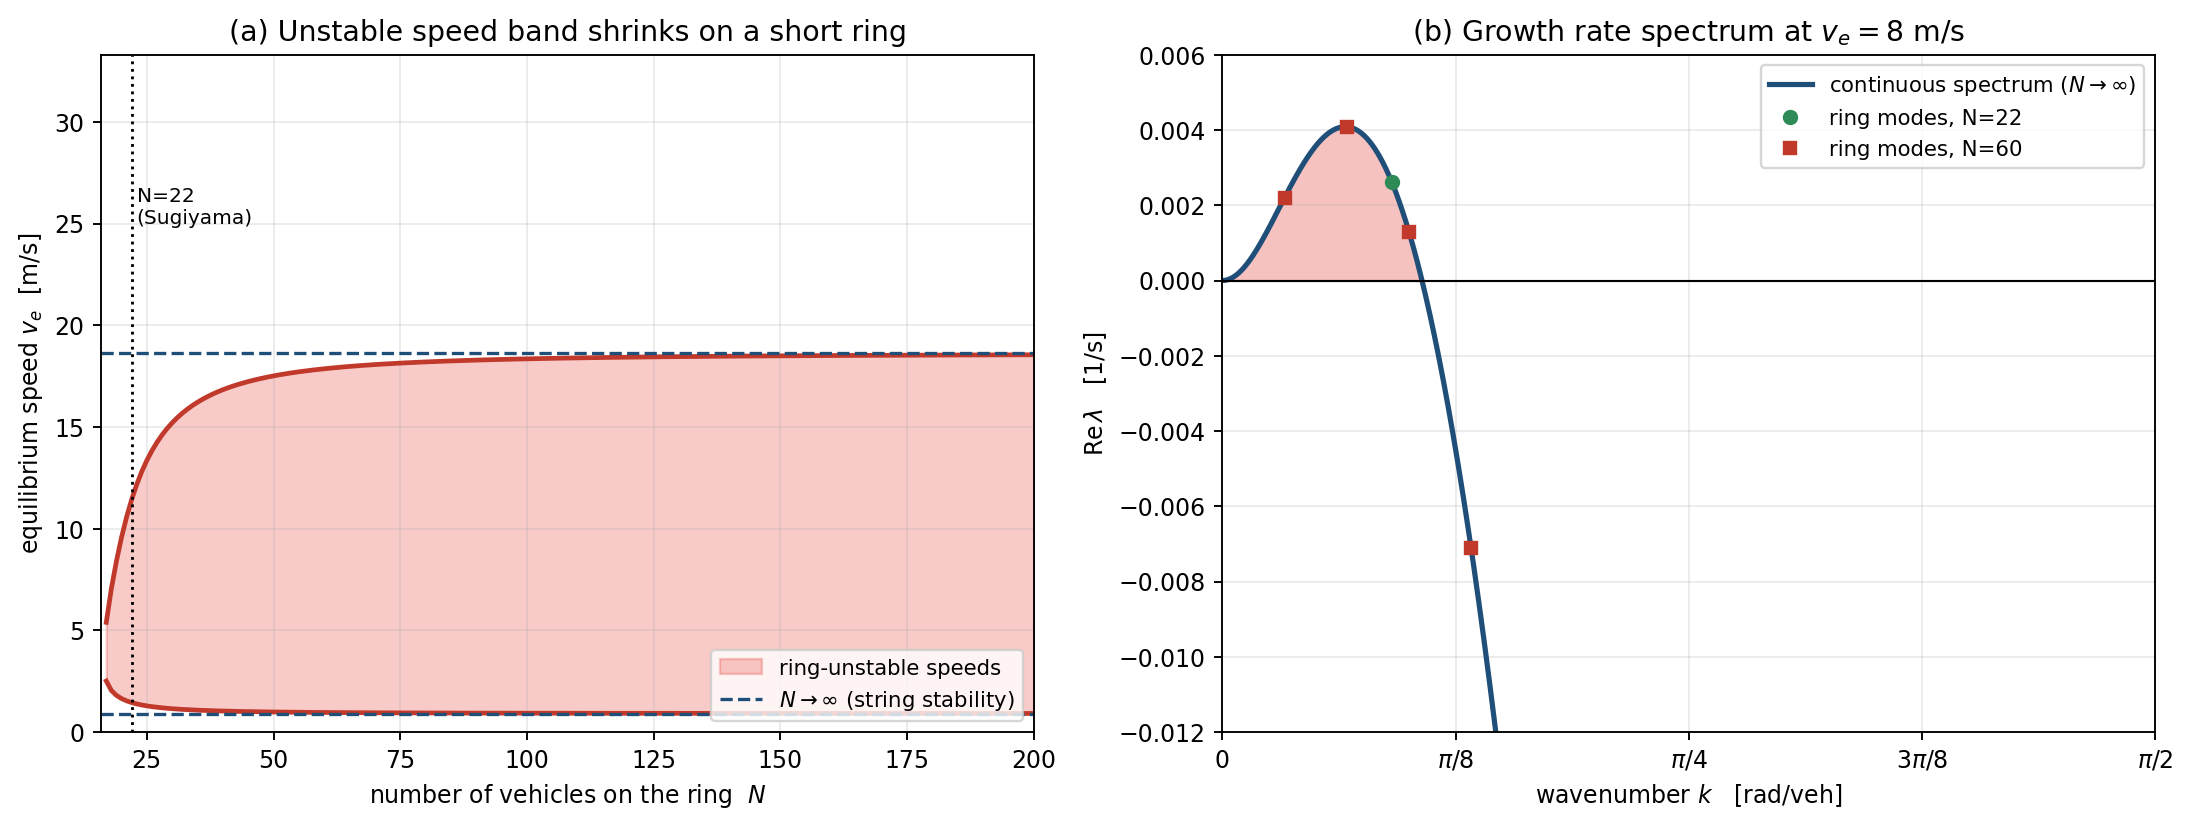
\includegraphics[width=\textwidth]{fig3.png}
\caption{The effect of limited loop size on discrete instability modes.}
\label{fig:finite-ring-band}
\figurenote{How the size of a finite ring track affects the observable instability band. The figure on the left shows the number of vehicles ($N$) gradually increasing on a very small ring track; the solid boundaries indicate the unstable speed range for each finite $N$, while the dashed lines represent the linear stability limits of $N\to\infty$; The range shrinks significantly for small circuits, and $N\le15$ even appears to be stable across the entire speed range under this parameter. In the right figure, $v_e=8$ (m/s) is fixed; the continuous curve represents the growth rate spectrum for arbitrary wave numbers, while the discrete markers indicate the actual values of $k_m=2\pi m/N$ achievable for specific loop sizes; the dangerous positive-growth region is confined to a very narrow range of small $k$ values. The lowest mode of $N=22$ is just at the edge of the positive growth region; therefore, it can only capture a portion of the instability band for an infinite train. As $N$ increases, the discrete points become denser toward zero wave number and gradually reproduce the continuous spectrum. This figure demonstrates that a finite loop track systematically overestimates stability because it fails to sample long waves; it also illustrates that the number of experimental vehicles must be reported as part of the stability results.}
\end{figure}

\begin{tcolorbox}[notebox,title=\textbf{Practical Reminder}]

Calibrating line stability thresholds using finite-loop simulations will




\textbf{systematically overestimate stability}




. The instability band calculated using $N=22$ (the scale of Sugiyama’s classic experiment) is only slightly more than half the actual value. To approximate linear stability, $N$ must be at least in the hundreds.







\end{tcolorbox}

\begin{tcolorbox}[resultbox,title=\textbf{Numerical Verification E5: Finite-Loop-Path Scan}]

The discrete spectrum was calculated one by one using $N=5,10,15,22,50,100$, yielding the following instability bands in order: stable across the entire speed range, stable across the entire speed range, stable across the entire speed range, $1.45$--$11.43$, $0.99$–$17.51$, $0.93$–$18.35$ m/s; the continuous limit is $0.91$–$18.61$ m/s. The results agree with $\cos(2\pi/N)$ in the closed-loop condition and quantify the error caused by the finite loop failing to sample dangerous long waves.







\end{tcolorbox}

\section{How to Choose Between the Two Methods}
\sectionstudy{synthesis}{How to Choose Between the Two Methods}{swaroop1996,ploeg2014,feng2019}

\begin{center}
\small
\captionof{table}{Comparison of the transfer function and the loop Fourier methods.}
\label{tab:transfer-versus-ring}
\begin{tabular}{p{3.0cm}p{5.4cm}p{5.4cm}}
\toprule
& \textbf{Transfer function $\left\|G\right\|_\infty\le1$} & \textbf{Ring-Space Fourier $+$} \\
\midrule







Scope of Application




&




 Limited to unidirectional cascaded coupling




&




 Any coupling configuration (including bidirectional and multiple lead vehicles)



\\[4pt]

Boundary Conditions




&




 Open chain with one lead vehicle




&




 Periodic boundary\\[4pt]

Questions Asked




&




At a fixed time frequency




\textbf{Along the spatial}




magnification factor




&




 At a fixed spatial wavenumber




\textbf{Over time}




Growth rate



\\[4pt]

Computational Complexity




&




A scalar inequality—the simplest case




&




Requires complex coefficients: Routh–Hurwitz (Bilharz)



\\[4pt]

Additional Information




&




 Vehicle-by-vehicle amplification factor, most dangerous frequency




&




 Growth rate $\operatorname{Re}\lambda(k)$, most unstable wavenumber (predictable stop-and-go wave wavelength)



\\
\bottomrule
\end{tabular}
\end{center}
\tabletext{tab:transfer-versus-ring}{




Applicable couplings, boundary conditions, problem types, and output quantities for the two stability methods. In a unidirectional homogeneous fleet, their boundaries are consistent; however, in bidirectional or multi-lead-vehicle configurations where the scalar cascade is disrupted, only the loop dispersion relation or the eigenvalues of the complete system can be used.
}










Conclusion:




\textbf{For unidirectional models, both methods are valid and yield identical boundary conditions at $N\to\infty$; the transfer function calculation is more straightforward, while the ring analysis has a broader scope of application and can simultaneously provide both the growth rate and the dominant wavenumber.} Once the coupling becomes bidirectional, the scalar per-vehicle transfer function is no longer applicable, and one should switch to a loop or system-wide eigenvalue analysis.




%==================================================================







\sectionwrapup{In a unidirectional, homogeneous convoy, the ring-track condition $G(\lambda)=e^{\mathrm{i}k}$ links the per-vehicle transfer function to the spatial modal; when $N\to\infty$ holds, both yield the same stability boundary. When bidirectional, heterogeneous, or nonlocal coupling disrupts the scalar cascade, ring-track or full-system eigenvalue analysis should be used instead.
}

\backmatter
\setcounter{secnumdepth}{-1}
\renewcommand{\chaptermark}[1]{\markboth{#1}{}}
\renewcommand{\sectionmark}[1]{\markright{#1}}
\chapter{Summary and Outlook}

\section{Overview of All Stability Conditions}
\sectionstudy{synthesis}{Overview of All Stability Conditions}{helbing2001,treiberkesting2013,ororsz2010}

\begin{center}
\scriptsize
\captionof{table}{Overview of Stability Conditions for the Reference and Extended Models.}
\label{tab:all-stability-conditions}
\begin{tabular}{p{1.8cm}p{2.9cm}p{3.4cm}p{3.2cm}p{2.5cm}}
\toprule
& \textbf{Reference Model} & \textbf{+ Leading Vehicle Acceleration} & \textbf{+ Leading and Trailing Vehicle Accelerations} & \textbf{+ Time Delay} \\
\midrule







Coupled Structures




&




 Unidirectional Cascading




&




 Unidirectional Cascading




& \textbf{Bidirectional (tri-diagonal)} &




 Arbitrary



\\[3pt]
$P(k)$ & $1$ & $1-f_ae^{-ik}$ & $1-f_ae^{-ik}-f_be^{ik}$ &




 Same as above, multiplied by a time delay factor



\\[3pt]

Characteristic Equation& Quadratic (real coefficients)




&




 Quadratic (complex coefficients)




&




 Quadratic (complex coefficients)




& \textbf{Polynomial} \\[3pt]

Locally stable




& $f_s>0,\ f_v<0$ &




 Identical




&




 Identical




&




 Added $\tau_0<\tau_0^{\rm crit}$



\\[3pt]

Wave speed $c_1$




& $V'(s_e)$ &




 Unchanged




&




 Unchanged




&




 Unchanged



\\[3pt]

Longwave conditions




& $\dfrac{f_v^2-f_{v_l}^2}{2}\ge f_s$
        & $\dfrac{f_v^2-f_{v_l}^2}{2}\ge(1-f_a)f_s$
        & $\dfrac{f_v^2-f_{v_l}^2}{2}\ge(1-\sigma_{\rm eff})f_s$
        & \textbf{Exactly the same as on the left} \\[10pt]

Additional conditions




&




 None




& $\left|f_a\right|\le1$
        &




 Internal check of $\left|\sigma_{\rm eff}\right|<1$ and $\widetilde W(u)>0$







&




 $\Psi(\omega)\ge0$ Full-band



\\[8pt]

Available methods




&




 Long-wave $=$ transfer function& \textbf{Must}




Transfer Function




& \textbf{Required}




Ring $+$ Bilharz




&




 Long-wave closed-form $+$ values



\\
\bottomrule
\end{tabular}
\end{center}
\tabletext{tab:all-stability-conditions}{




Correlations between the reference model, lead-vehicle feedback, bidirectional feedback, and time delay in terms of coupled structures, characteristic equations, local/long-wave conditions, and additional constraints. This serves as a reference index for criteria throughout the book but does not replace the derivations of finite-wavelength and delayed full-frequency-band conditions presented in each chapter.
}

\section{Heterogeneous Vehicle Convoys (Chapter ~\ref{sec:het}~)
}
\sectionstudy{theory}{




Heterogeneous Vehicle Flocks (Chapter ~\ref{sec:het}~)
}{helbing2001,treiberkesting2013,ororsz2010}

\begin{tcolorbox}[keybox]
\begin{itemize}[leftmargin=1.6em,itemsep=4pt]
\item




 The steady-state condition is modified to




\textbf{Same Speed, Different Distances}




; Spatial Fourier analysis fails, and the transfer function becomes the only useful tool (the exact opposite of bidirectional coupling).







\item




 Chain product $\hat y_j/\hat y_0=\prod_{n\le j}G_n$; the loop characteristic equation is $\prod_{n=1}^N G_n(\lambda)=1$.







\item




 The long-wave condition becomes




\textbf{Weighted prefix sum} $\sum_{n\le j}\eta_n\ge0$, weight $1/f_s^2$—sluggish cars ($f_s$ is small) have an extremely high weight.







\item \textbf{When the circuit is closed, only $j=N$ is checked; when the circuit is open and there is no amplification within the pack, all $j$ are checked.}




: When $G_n$ is fixed, the lap-time product is independent of the order, but the mid-lap prefix gain is strongly dependent on the order.







\item




 In this example of hybrid autonomous driving: when $\kappa=0.5$ is set, the total budget threshold for the entire formation/circuit long wave is $26.7\%$, and is approximately inversely proportional to $\kappa$; this number itself does not guarantee that any arrangement will satisfy the prefix conditions.







\item




If an AV’s feedforward capability




\textbf{depends on the type of the leading vehicle}




(V2V requires the leading vehicle to also be an AV), then $\eta_n$ depends on adjacent pairs,




\textbf{and even the sum becomes dependent on the order}




: For dispersed vehicles, $89.1\%$ must be applied; for grouped formations, only $26.7\%$ is needed. The optimal solution is to select the




\textbf{maximum number of groups that satisfies $n_{\rm grp}\le n_{\rm grp}^{\max}$}—First, ensure the long-wave budget is maintained, then diversify as much as possible.







\end{itemize}
\end{tcolorbox}

\section{Three Key “Invariants”}
\sectionstudy{synthesis}{Three Key “Invariants”}{helbing2001,treiberkesting2013,ororsz2010}

\begin{tcolorbox}[keybox]
\begin{enumerate}[leftmargin=1.6em,itemsep=4pt]
\item \textbf{Local stability is not affected by the neighboring vehicle acceleration feedback considered in this book.}




When the leading and trailing vehicles are traveling at constant speeds, these terms are always zero, and pure feedforward does not enter the vehicle’s closed-loop system; reaction delay, however, introduces an additional upper bound on local stability.







\item \textbf{Acceleration feedback does not alter the kinematic wave speed.}




In Chapters ~\ref{sec:lead}~ through ~\ref{sec:multi}~, $c_1=V'(s_e)$ holds at all times; backward spacing feedback (Chapters ~\ref{sec:reargap}~) yields $c_1=(1-h_s/f_s)V'$, which tends to zero in the limit of perfect symmetry.







\item \textbf{The long-wave threshold is determined solely by the zero-order moment $m_0$.}




Within the framework of this book’s model, the spatial distribution of forward/backward views, the number of observed vehicles, and the delay do not alter this threshold. Therefore, control design can first determine the total gain budget and then verify the constraints on finite wavelength and delay.







\end{enumerate}
\end{tcolorbox}

\section{Summary of Numerical Results for the IDM Example}
\sectionstudy{experiment}{Summary of Numerical Results for the IDM Example}{treiber2000,treiberkesting2013}





Parameters: $v_0=33.3$ m/s, $T=1.5$ s, $s_0=2$ m, $a=1$ m/s, $^2$, $b=1.5$ m/s, $^2$, $\delta=4$, $l=5$ m.










\begin{center}
\small
\captionof{table}{Key values for the reference IDM case.}
\label{tab:idm-number-summary}
\begin{tabular}{p{6.4cm}p{7.4cm}}
\toprule







Reference unstable speed band




& $0.91$ -- $18.61$ m/s（$\rho=27.4$--$119.6$ veh/km） \\







Most unstable point




& $v_e\approx3.1$ m/s，$\Phi_{\min}=-0.027$ \\







Congestion limit criterion




&




 $aT^2/s_0=1.125>1$; therefore, the system is stable at $v_e\to0$



\\
\midrule







Critical gain for lead vehicle acceleration feedforward




&




 $\kappa_c=0.134$ (upper bound is 1, with sufficient margin)



\\







Nearest-neighbor gain required for multiple leading vehicles ($\alpha=0.8$)




&




 $f_a=0.027$, i.e., diluted by a factor of $1/(1-\alpha)$



\\







Available window for pure lookback ($f_b>0,\beta=0$)& $0.134\le f_b\le0.43$; $\beta\gtrsim0.58$—no solution



\\
\midrule







Reaction delay: Local stability upper bound




& $\tau_0^{\rm crit}=1.16$ s（$v_e=2$）$\sim$ $2.52$ s（$v_e=20$） \\







Reaction delay widens the instability band




&




 At $\tau_0=1.5$ s, expands to $0$–$25.98$ m/s



\\







Communication delay compresses the gain window




&




 At $\tau_a=1.5$ s, the upper bound of $\kappa$ decreases from $1.00$ to $0.60$, while the lower bound remains constant at $0.134$



\\
\midrule







Critical Weight for Backward Spacing Feedback




& $p_c=0.223$（$h_s=pf_s,\ h_v=pf_{v_l}$） \\







Instability Band for the Finite Loop $N=22$




&




$1.45$–$11.43$ m/s (slightly more than half the true value)



\\
\bottomrule
\end{tabular}
\end{center}
\tabletext{tab:idm-number-summary}{




Instability Speed Bands, Critical Feedback Gain, Delay Window, Lookback Threshold, and Finite Loop Deviation for the Reference IDM. This table consolidates representative figures scattered throughout the chapters in one place; specific definitions, applicable conditions, and reproducibility experiments should still be referenced in the corresponding chapters.
}

\section{Nonlinear, Learning-Based Models, and Application Conclusions}
\sectionstudy{application}{Nonlinear, Learning-Based Models and Application Conclusions}{ororsz2010,wang2025kidl,chang2019neural}

\begin{tcolorbox}[keybox]
\begin{itemize}[leftmargin=1.5em,itemsep=4pt]
\item




 The unified weakly nonlinear normal form of the original IDM near the neutral line is of the Gardner–Burgers type: the sign of the diffusion coefficient is determined by the linear long-wave margin, quadratic/cubic nonlinearity determines the steepening of the waveform, and the $O(k^3)$ term provides dispersion.







\item




Neither of the two neutral boundaries of the reference IDM strictly satisfies $V''=0$, so the pure mKdV equation is not a general conclusion; the lower boundary $V''$ is very small, so using the Gardner equation is more reliable than simply discarding the quadratic term.







\item




$v_e=8$ m/s, and the $0.02$ m/ s amplifies $\sigma_v$ from $0.01414$ to $2.962$ m/s within 1800 s and causes a noticeable steepening of the waveform; The same perturbation at $v_e=20$ m/s, however, decreased to $3.27\times10^{-8}$ m/s.







\item




From D01 of NGSIM US--101, 78 consecutive tracking segments were extracted from 39,187 records: the median empirical gain was $1.033$, but the 95% bootstrap\% The fact that the $[0.954,1.077]$ interval crosses 1 indicates that amplification and attenuation coexist in the real-world data; therefore, a single spatiotemporal plot cannot be directly interpreted as proof of overall instability.







\item




 D02 Extend the application of real-world data to a closed-loop “calibration—validation—optimization” process: Compared to fitting a single following vehicle, the fleet stability calibration reduces the RMSE for speed and distance in the reserved segment by $69.6\%$ and $34.4\%$, respectively; subsequently, $\kappa=0.04$ is selected based on spectral constraints at the worst-case experienced speed. This control gain is a counterfactual result based on the calibrated model and is not equivalent to the verified gain on real roads.







\item




 Stability analysis can directly support CACC gains, AV penetration rates/convoys, online early warnings, loop road scale, parameter calibration, and robust operation design; During application, local roots, propagation amplification, finite-amplitude responses, and numerical convergence must all be verified simultaneously.







\item




Learning-based followers can restore equilibrium gradients via automatic differentiation; RNNs/GNNs require expanded hidden states or full-graph Jacobians, while reinforcement learning strategies must include vehicles, observations, delays, and saturation checks to ensure a complete closed-loop system. Training convergence, low RMSE, and high rewards cannot, on their own, constitute evidence of traffic flow stability.







\end{itemize}
\end{tcolorbox}

\newpage
\section{Engineering Key Points}
\sectionstudy{theory}{Engineering Key Points}{helbing2001,treiberkesting2013,ororsz2010}

\begin{itemize}[leftmargin=1.4em,itemsep=4pt]
\item \textbf{Determine the total budget first, then decide on the allocation.}




Calculate the required $\sigma_{\rm eff}$ ($0.134$ in this example) using long-wave conditions; this step is unrelated to delay, apportionment, or forward-backward allocation.


\item \textbf{Forward allocation does not reduce the long-wavelength margin; backward allocation requires an additional check for finite wavelengths.}




 The nearest-neighbor gain in the forward direction may decrease linearly according to $(1-\alpha)$; under the forward-looking convention used in this example, $\beta$ should not exceed approximately $0.5$. If the backward-looking convention commonly found in the literature is adopted, the conclusion will change accordingly (




\S\ref{sub:negfb}）。
\item \textbf{Delay does not alter the long-wave threshold but narrows the available gain range.}




 In the vicinity of this set of parameters, for every increase in communication delay of approximately $0.5$ s, the upper bound on available gain decreases by approximately $0.1$–$0.2$; reaction delay is generally more detrimental, while at $\tau_a\approx\tau_0$, certain phase effects may partially offset this.







\item \textbf{Stabilization and wave speed control are two distinct objectives.}




Acceleration feedback can improve the stability margin without altering $c_1$; backward spacing feedback affects both simultaneously. In this example, $p_c=0.223$ indicates that the unstable velocity band is just closed, at which point $c_1=(1-p_c)V'$ is still nonzero; the wave velocity approaches zero only in the fully symmetric limit $p\to1$.







\item \textbf{Do not use short ring tracks to calibrate thresholds.} $N=22$ systematically overestimates stability; to approximate linear stability, $N$ must be at least in the hundreds.







\end{itemize}

\section{Scope of Application and Follow-up}
\sectionstudy{synthesis}{Scope of Application and Follow-up}{helbing2001,treiberkesting2013,ororsz2010}

\begin{tcolorbox}[notebox]

Chapter ~\ref{sec:nonlinear}~ has extended the original IDM to




\textbf{the level of weak nonlinearity}




level, capable of explaining diffusion, dispersion, wave steepening near the neutral line, and the KdV/mKdV/Gardner reduction conditions; however, this book still does not claim to provide a global stability proof under arbitrary finite-amplitude perturbations. Issues not yet covered include:







\begin{itemize}[leftmargin=1.2em,itemsep=2pt]
\item




 Rigorously identifying, using bidirectional continuation or bifurcation software,




\textbf{subcritical bifurcations}




, coexisting attractors, and hysteresis loops under finite-amplitude perturbations;







\item




 Rededuce the respective nonlinear normal forms for models containing feedforward, lookback, time delays, and heterogeneity;







\item




Stability under the combined effects of lane changes, ramps, stochastic driving, communication packet loss, and discrete controllers;







\item




 Conduct systematic statistical tests of nonlinear amplitude relationships against measured trajectory data, rather than relying solely on a single set of simulation comparisons.







\item




Extend the local Jacobian diagnosis from Chapter ~\ref{sec:ml-stability}~ to scalable closed-loop certification that accounts for model errors, stochastic policies, and large-scale attention networks.


\end{itemize}


These problems require tools for system-wide numerical continuity, stochastic stability, or mixed-system analysis, which go beyond the single-path deterministic framework of this book.







\end{tcolorbox}

\section{Summary of the Book}
\sectionstudy{synthesis}{Summary of the Book}{helbing2001,treiberkesting2013,ororsz2010}










This book establishes a complete hierarchy ranging from local roots of a single vehicle, fleet interactions, ring-track modes, and finite-amplitude waveforms to macroscopic continuous flow, adaptive dynamics, and engineering control. When using any “stable” conclusion, one must simultaneously specify the model or network architecture, steady-state conditions, perturbation scale, boundary conditions, permissible wave numbers, sampling method, and numerical accuracy; only when these conditions are consistent can theoretical criteria, simulation results, empirical evidence, and traffic management implications be mutually validated.





\clearpage
\begin{thebibliography}{99}
\bibitem{chandler1958}
Robert E. Chandler, Robert Herman, and Elliott W. Montroll,
{Traffic dynamics: Studies in car following},
\emph{Operations Research}, vol.~6, no.~2, pp.~165--184, 1958.
\href{https://doi.org/10.1287/opre.6.2.165}{doi:10.1287/opre.6.2.165}.

\bibitem{gazis1961}
Denos C. Gazis, Robert Herman, and Richard W. Rothery,
{Nonlinear follow-the-leader models of traffic flow},
\emph{Operations Research}, vol.~9, no.~4, pp.~545--567, 1961.
\href{https://doi.org/10.1287/opre.9.4.545}{doi:10.1287/opre.9.4.545}.

\bibitem{bando1995}
Masako Bando, Katsuya Hasebe, Akihiro Nakayama, Akihiro Shibata, and Yuki Sugiyama,
{Dynamical model of traffic congestion and numerical simulation},
\emph{Physical Review E}, vol.~51, no.~2, pp.~1035--1042, 1995.
\href{https://doi.org/10.1103/PhysRevE.51.1035}{doi:10.1103/PhysRevE.51.1035}.

\bibitem{treiber2000}
Martin Treiber, Ansgar Hennecke, and Dirk Helbing,
{Congested traffic states in empirical observations and microscopic simulations},
\emph{Physical Review E}, vol.~62, no.~2, pp.~1805--1824, 2000.
\href{https://doi.org/10.1103/PhysRevE.62.1805}{doi:10.1103/PhysRevE.62.1805}.

\bibitem{lighthill1955}
M. J. Lighthill and G. B. Whitham,
``On kinematic waves II. A theory of traffic flow on long crowded roads,''
\emph{Proceedings of the Royal Society A}, vol.~229, no.~1178, pp.~317--345, 1955.
\href{https://doi.org/10.1098/rspa.1955.0089}{doi:10.1098/rspa.1955.0089}.

\bibitem{richards1956}
Paul I. Richards,
``Shock waves on the highway,''
\emph{Operations Research}, vol.~4, no.~1, pp.~42--51, 1956.
\href{https://doi.org/10.1287/opre.4.1.42}{doi:10.1287/opre.4.1.42}.

\bibitem{payne1971}
Harold J. Payne,
``Models of freeway traffic and control,''
in \emph{Mathematical Models of Public Systems}, vol.~1, pp.~51--61, 1971.

\bibitem{daganzo1995}
Carlos F. Daganzo,
``Requiem for second-order fluid approximations of traffic flow,''
\emph{Transportation Research Part B: Methodological}, vol.~29, no.~4, pp.~277--286, 1995.
\href{https://doi.org/10.1016/0191-2615(95)00007-Z}{doi:10.1016/0191-2615(95)00007-Z}.

\bibitem{awrascle2000}
Awatif Aw and Michel Rascle,
``Resurrection of `second order' models of traffic flow,''
\emph{SIAM Journal on Applied Mathematics}, vol.~60, no.~3, pp.~916--938, 2000.
\href{https://doi.org/10.1137/S0036139997332099}{doi:10.1137/S0036139997332099}.

\bibitem{zhang2002}
H. Michael Zhang,
``A non-equilibrium traffic model devoid of gas-like behavior,''
\emph{Transportation Research Part B: Methodological}, vol.~36, no.~3, pp.~275--290, 2002.
\href{https://doi.org/10.1016/S0191-2615(00)00050-3}{doi:10.1016/S0191-2615(00)00050-3}.

\bibitem{jin2003}
Wen-Long Jin and H. Michael Zhang,
``The formation and structure of vehicle clusters in the Payne--Whitham traffic flow model,''
\emph{Transportation Research Part B: Methodological}, vol.~37, no.~3, pp.~207--223, 2003.
\href{https://doi.org/10.1016/S0191-2615(02)00008-5}{doi:10.1016/S0191-2615(02)00008-5}.

\bibitem{ngsim2016}
U.S. Department of Transportation, Federal Highway Administration,
\emph{Next Generation Simulation (NGSIM) Vehicle Trajectories and Supporting Data},
dataset, 2016, accessed 2026-08-28.
\href{https://doi.org/10.21949/1504477}{doi:10.21949/1504477}.

\bibitem{savitzky1964}
Abraham Savitzky and Marcel J. E. Golay,
``Smoothing and differentiation of data by simplified least squares procedures,''
\emph{Analytical Chemistry}, vol.~36, no.~8, pp.~1627--1639, 1964.
\href{https://doi.org/10.1021/ac60214a047}{doi:10.1021/ac60214a047}.

\bibitem{wu2015ev}
Xinkai Wu, David Freese, Alfredo Cabrera, and William A. Kitch,
``Electric vehicles' energy consumption measurement and estimation,''
\emph{Transportation Research Part D: Transport and Environment}, vol.~34, pp.~52--67, 2015.
\href{https://doi.org/10.1016/j.trd.2014.10.007}{doi:10.1016/j.trd.2014.10.007}.

\bibitem{newell1961}
Gordon F. Newell,
``Nonlinear effects in the dynamics of car following,''
\emph{Operations Research}, vol.~9, no.~2, pp.~209--229, 1961.
\href{https://doi.org/10.1287/opre.9.2.209}{doi:10.1287/opre.9.2.209}.

\bibitem{gipps1981}
Peter G. Gipps,
``A behavioural car-following model for computer simulation,''
\emph{Transportation Research Part B: Methodological}, vol.~15, no.~2, pp.~105--111, 1981.
\href{https://doi.org/10.1016/0191-2615(81)90037-0}{doi:10.1016/0191-2615(81)90037-0}.

\bibitem{jiang2001}
Rui Jiang, Qing-Song Wu, and Zuo-Jin Zhu,
``Full velocity difference model for a car-following theory,''
\emph{Physical Review E}, vol.~64, 017101, 2001.
\href{https://doi.org/10.1103/PhysRevE.64.017101}{doi:10.1103/PhysRevE.64.017101}.

\bibitem{helbing2001}
Dirk Helbing,
``Traffic and related self-driven many-particle systems,''
\emph{Reviews of Modern Physics}, vol.~73, no.~4, pp.~1067--1141, 2001.
\href{https://doi.org/10.1103/RevModPhys.73.1067}{doi:10.1103/RevModPhys.73.1067}.

\bibitem{treiberkesting2013}
Martin Treiber and Arne Kesting,
\emph{Traffic Flow Dynamics: Data, Models and Simulation},
Springer, Berlin, 2013.
\href{https://doi.org/10.1007/978-3-642-32460-4}{doi:10.1007/978-3-642-32460-4}.

\bibitem{wilsonward2011}
R. Eddie Wilson and Jonathan A. Ward,
``Car-following models: Fifty years of linear stability analysis---a mathematical perspective,''
\emph{Transportation Planning and Technology}, vol.~34, no.~1, pp.~3--18, 2011.
\href{https://doi.org/10.1080/03081060.2011.530826}{doi:10.1080/03081060.2011.530826}.

\bibitem{swaroop1996}
D. Swaroop and J. Karl Hedrick,
``String stability of interconnected systems,''
\emph{IEEE Transactions on Automatic Control}, vol.~41, no.~3, pp.~349--357, 1996.
\href{https://doi.org/10.1109/9.486636}{doi:10.1109/9.486636}.

\bibitem{ploeg2014}
Jeroen Ploeg, Nathan van de Wouw, and Henk Nijmeijer,
``$L_p$ string stability of cascaded systems: Application to vehicle platooning,''
\emph{IEEE Transactions on Control Systems Technology}, vol.~22, no.~2, pp.~786--793, 2014.
\href{https://doi.org/10.1109/TCST.2013.2258346}{doi:10.1109/TCST.2013.2258346}.

\bibitem{stuedli2017}
Sonja St\"udli, María M. Seron, and Richard H. Middleton,
``From vehicular platoons to general networked systems: String stability and related concepts,''
\emph{Annual Reviews in Control}, vol.~44, pp.~157--172, 2017.
\href{https://doi.org/10.1016/j.arcontrol.2017.09.016}{doi:10.1016/j.arcontrol.2017.09.016}.

\bibitem{feng2019}
Shuo Feng, Yi Zhang, Shengbo Eben Li, Zhong Cao, Henry X. Liu, and Li Li,
``String stability for vehicular platoon control: Definitions and analysis methods,''
\emph{Annual Reviews in Control}, vol.~47, pp.~81--97, 2019.
\href{https://doi.org/10.1016/j.arcontrol.2019.03.001}{doi:10.1016/j.arcontrol.2019.03.001}.

\bibitem{dunbar2012}
William B. Dunbar and Derek S. Caveney,
``Distributed receding horizon control of vehicle platoons: Stability and string stability,''
\emph{IEEE Transactions on Automatic Control}, vol.~57, no.~3, pp.~620--633, 2012.
\href{https://doi.org/10.1109/TAC.2011.2159651}{doi:10.1109/TAC.2011.2159651}.

\bibitem{ororsz2004}
Gábor Orosz, R. Eddie Wilson, and Bernd Krauskopf,
``Global bifurcation investigation of an optimal velocity traffic model with driver reaction time,''
\emph{Physical Review E}, vol.~70, 026207, 2004.
\href{https://doi.org/10.1103/PhysRevE.70.026207}{doi:10.1103/PhysRevE.70.026207}.

\bibitem{ororsz2010}
Gábor Orosz, R. Eddie Wilson, and Gábor Stépán,
``Traffic jams: Dynamics and control,''
\emph{Philosophical Transactions of the Royal Society A}, vol.~368, no.~1928, pp.~4455--4479, 2010.
\href{https://doi.org/10.1098/rsta.2010.0205}{doi:10.1098/rsta.2010.0205}.

\bibitem{lenz1999}
Hanno Lenz, Christian K. Wagner, and Ralf Sollacher,
``Multi-anticipative car-following model,''
\emph{The European Physical Journal B}, vol.~7, no.~2, pp.~331--335, 1999.
\href{https://doi.org/10.1007/s100510050618}{doi:10.1007/s100510050618}.

\bibitem{sugiyama2008}
Yuki Sugiyama, Minoru Fukui, Macoto Kikuchi, Katsuya Hasebe, Akihiro Nakayama,
Katsuhiro Nishinari, Shin-ichi Tadaki, and Satoshi Yukawa,
``Traffic jams without bottlenecks---experimental evidence for the physical mechanism of the formation of a jam,''
\emph{New Journal of Physics}, vol.~10, 033001, 2008.
\href{https://doi.org/10.1088/1367-2630/10/3/033001}{doi:10.1088/1367-2630/10/3/033001}.

\bibitem{treiberkesting2011}
Martin Treiber and Arne Kesting,
``Evidence of convective instability in congested traffic flow: A systematic empirical and theoretical investigation,''
\emph{Transportation Research Part B: Methodological}, vol.~45, no.~9, pp.~1362--1377, 2011.
\href{https://doi.org/10.1016/j.trb.2011.05.011}{doi:10.1016/j.trb.2011.05.011}.

\bibitem{milanes2014}
Vicente Milanés, Steven E. Shladover, John Spring, Christopher Nowakowski,
Hiroshi Kawazoe, and Masahide Nakamura,
``Cooperative adaptive cruise control in real traffic situations,''
\emph{IEEE Transactions on Intelligent Transportation Systems}, vol.~15, no.~1, pp.~296--305, 2014.
\href{https://doi.org/10.1109/TITS.2013.2278494}{doi:10.1109/TITS.2013.2278494}.

\bibitem{talebpour2016}
Alireza Talebpour and Hani S. Mahmassani,
``Influence of connected and autonomous vehicles on traffic flow stability and throughput,''
\emph{Transportation Research Part C: Emerging Technologies}, vol.~71, pp.~143--163, 2016.
\href{https://doi.org/10.1016/j.trc.2016.07.007}{doi:10.1016/j.trc.2016.07.007}.

\bibitem{stern2018}
Raphael E. Stern, Shumo Cui, Maria Laura Delle Monache, Rahul Bhadani,
Matt Bunting, Miles Churchill, et al.,
``Dissipation of stop-and-go waves via control of autonomous vehicles: Field experiments,''
\emph{Transportation Research Part C: Emerging Technologies}, vol.~89, pp.~205--221, 2018.
\href{https://doi.org/10.1016/j.trc.2018.02.005}{doi:10.1016/j.trc.2018.02.005}.

\bibitem{komatsu1995}
Teruhisa S. Komatsu and Shin-ichi Sasa,
``A kink soliton characterizing traffic congestion,''
\emph{Physical Review E}, vol.~52, no.~5, pp.~5574--5582, 1995.
\href{https://doi.org/10.1103/PhysRevE.52.5574}{doi:10.1103/PhysRevE.52.5574}.

\bibitem{leveque2002}
Randall J. LeVeque,
\emph{Finite Volume Methods for Hyperbolic Problems},
Cambridge University Press, Cambridge, 2002.
\href{https://doi.org/10.1017/CBO9780511791253}{doi:10.1017/CBO9780511791253}.

\bibitem{kesting2008}
Arne Kesting and Martin Treiber,
``Calibrating car-following models by using trajectory data: Methodological study,''
\emph{Transportation Research Record}, no.~2088, pp.~148--156, 2008.
\href{https://doi.org/10.3141/2088-16}{doi:10.3141/2088-16}.

\bibitem{ossen2009}
Saskia Ossen and Serge P. Hoogendoorn,
``Reliability of parameter values estimated using trajectory observations,''
\emph{Transportation Research Record}, no.~2124, pp.~36--44, 2009.
\href{https://doi.org/10.3141/2124-04}{doi:10.3141/2124-04}.

\bibitem{punzo2012}
Vincenzo Punzo, Biagio Ciuffo, and Marcello Montanino,
``Can results of car-following model calibration based on trajectory data be trusted?''
\emph{Transportation Research Record}, no.~2315, pp.~11--24, 2012.
\href{https://doi.org/10.3141/2315-02}{doi:10.3141/2315-02}.

\bibitem{thiemann2008}
Christian Thiemann, Martin Treiber, and Arne Kesting,
``Estimating acceleration and lane-changing dynamics from Next Generation Simulation trajectory data,''
\emph{Transportation Research Record}, no.~2088, pp.~90--101, 2008.
\href{https://doi.org/10.3141/2088-10}{doi:10.3141/2088-10}.

\bibitem{krajewski2018}
Robert Krajewski, Julian Bock, Laurent Kloeker, and Lutz Eckstein,
``The highD dataset: A drone dataset of naturalistic vehicle trajectories on German highways for validation of highly automated driving systems,''
in \emph{2018 IEEE 21st International Conference on Intelligent Transportation Systems}, pp.~2118--2125, 2018.
\href{https://doi.org/10.1109/ITSC.2018.8569552}{doi:10.1109/ITSC.2018.8569552}.

\bibitem{hegyi2005}
Andreas Hegyi, Bart De Schutter, and J. Hellendoorn,
``Optimal coordination of variable speed limits to suppress shock waves,''
\emph{IEEE Transactions on Intelligent Transportation Systems}, vol.~6, no.~1, pp.~102--112, 2005.
\href{https://doi.org/10.1109/TITS.2004.842408}{doi:10.1109/TITS.2004.842408}.

\bibitem{carlson2010}
Rodrigo C. Carlson, Ioannis Papamichail, Markos Papageorgiou, and Albert Messmer,
``Optimal motorway traffic flow control involving variable speed limits and ramp metering,''
\emph{Transportation Science}, vol.~44, no.~2, pp.~238--253, 2010.
\href{https://doi.org/10.1287/trsc.1090.0314}{doi:10.1287/trsc.1090.0314}.

\bibitem{chen2018neuralode}
Ricky T. Q. Chen, Yulia Rubanova, Jesse Bettencourt, and David K. Duvenaud,
``Neural ordinary differential equations,''
in \emph{Advances in Neural Information Processing Systems 31}, pp.~6571--6583, 2018.
\href{https://proceedings.neurips.cc/paper/2018/hash/69386f6bb1dfed68692a24c8686939b9-Abstract.html}{NeurIPS proceedings}.

\bibitem{bai2019deq}
Shaojie Bai, J. Zico Kolter, and Vladlen Koltun,
``Deep equilibrium models,''
in \emph{Advances in Neural Information Processing Systems 32}, 2019.
\href{https://proceedings.neurips.cc/paper/2019/hash/01386bd6d8e091c2ab4c7c7de644d37b-Abstract.html}{NeurIPS proceedings}.

\bibitem{miyato2018spectral}
Takeru Miyato, Toshiki Kataoka, Masanori Koyama, and Yuichi Yoshida,
``Spectral normalization for generative adversarial networks,''
in \emph{International Conference on Learning Representations}, 2018.
\href{https://arxiv.org/abs/1802.05957}{arXiv:1802.05957}.

\bibitem{revay2020contracting}
Max Revay and Ian Manchester,
``Contracting implicit recurrent neural networks: Stable models with improved trainability,''
in \emph{Proceedings of the 2nd Conference on Learning for Dynamics and Control},
PMLR, vol.~120, pp.~393--403, 2020.
\href{https://proceedings.mlr.press/v120/revay20a.html}{PMLR:120:393--403}.

\bibitem{chang2019neural}
Ya-Chien Chang, Nima Roohi, and Sicun Gao,
``Neural Lyapunov control,''
in \emph{Advances in Neural Information Processing Systems 32}, pp.~3240--3249, 2019.
\href{https://proceedings.neurips.cc/paper/2019/hash/2647c1dba23bc0e0f9cdf75339e120d2-Abstract.html}{NeurIPS proceedings}.

\bibitem{fazlyab2022}
Mahyar Fazlyab, Manfred Morari, and George J. Pappas,
``Safety verification and robustness analysis of neural networks via quadratic constraints and semidefinite programming,''
\emph{IEEE Transactions on Automatic Control}, vol.~67, no.~1, pp.~1--15, 2022.
\href{https://doi.org/10.1109/TAC.2020.3046193}{doi:10.1109/TAC.2020.3046193}.

\bibitem{raissi2019pinn}
Maziar Raissi, Paris Perdikaris, and George E. Karniadakis,
``Physics-informed neural networks: A deep learning framework for solving forward and inverse problems involving nonlinear partial differential equations,''
\emph{Journal of Computational Physics}, vol.~378, pp.~686--707, 2019.
\href{https://doi.org/10.1016/j.jcp.2018.10.045}{doi:10.1016/j.jcp.2018.10.045}.

\bibitem{brunton2016sindy}
Steven L. Brunton, Joshua L. Proctor, and J. Nathan Kutz,
``Discovering governing equations from data by sparse identification of nonlinear dynamical systems,''
\emph{Proceedings of the National Academy of Sciences}, vol.~113, no.~15, pp.~3932--3937, 2016.
\href{https://doi.org/10.1073/pnas.1517384113}{doi:10.1073/pnas.1517384113}.

\bibitem{lusch2018koopman}
Bethany Lusch, J. Nathan Kutz, and Steven L. Brunton,
``Deep learning for universal linear embeddings of nonlinear dynamics,''
\emph{Nature Communications}, vol.~9, 4950, 2018.
\href{https://doi.org/10.1038/s41467-018-07210-0}{doi:10.1038/s41467-018-07210-0}.

\bibitem{kreidieh2018drl}
Abdul Rahman Kreidieh, Cathy Wu, and Alexandre M. Bayen,
``Dissipating stop-and-go waves in closed and open networks via deep reinforcement learning,''
in \emph{2018 IEEE 21st International Conference on Intelligent Transportation Systems}, pp.~1475--1480, 2018.
\href{https://doi.org/10.1109/ITSC.2018.8569485}{doi:10.1109/ITSC.2018.8569485}.

\bibitem{wang2025kidl}
Chengming Wang, Dongyao Jia, Wei Wang, Dong Ngoduy, Bei Peng, and Jianping Wang,
``A knowledge-informed deep learning paradigm for generalizable and stability-optimized car-following models,''
\emph{Communications in Transportation Research}, vol.~5, 100211, 2025.
\href{https://doi.org/10.1016/j.commtr.2025.100211}{doi:10.1016/j.commtr.2025.100211}.
\end{thebibliography}

\end{document}
